\documentclass[11pt,openany,leqno]{book} % oneside twoside / report book / openany - bibl nie musi rozpoczynać się od nieparzystej
\usepackage[X2,T1]{fontenc}
\usepackage[utf8]{inputenc}
\usepackage{setspace}

\raggedbottom %usuwa przerwy między akapitami, spowodowane przez klasę book
\frenchspacing %usuwa podwójną przerwę po krpoce (zdaniu)

\usepackage{pdfpages}








\usepackage{graphicx}
%\usepackage{epic}
\usepackage{color}
\usepackage{amsmath}
\usepackage{bm}	% \boldsymbol
%\usepackage{amsbsy}	% \boldsymbol
\usepackage{amscd}	% diagramy
\usepackage{amsfonts}	% fonty
\usepackage{amssymb}	% dodatek math
\usepackage{amstext}	% \text
\usepackage{amsthm}
\usepackage{amsmath}
\usepackage{xfrac} %\sfrac{1}{2}
%\usepackage{nicefrac} %\nicefrac{1}{2}
\usepackage[normalem]{ulem}





\usepackage{longtable}
\usepackage{tabularx}
\renewcommand{\tabularxcolumn}[1]{m{#1}}
\newcolumntype{Y}{>{\centering\arraybackslash}X}
\newcolumntype{s}{>{\hsize=.8\hsize}X}
\renewcommand\arraystretch{1.2}
\usepackage{float} %umożliwia hard positioning (flaga: H)
\usepackage{supertabular}


\usepackage{array}
\usepackage{ragged2e}

%\newcolumntype{L}[1]{>{\RaggedRight\arraybackslash}m{#1}}
\newcolumntype{L}[1]{>{\RaggedRight\let\newline\arraybackslash}m{#1}}

\usepackage{adjustbox}




%Equation z marginesami
\usepackage{environ}
\makeatletter
\NewEnviron{widerequation}{%
	\begin{equation*}
	\sbox\z@{\let\label\@gobble$\displaystyle\BODY$}
	\makebox[\textwidth]{%
		\begin{minipage}{\dimexpr\wd\z@+3em}
		\vspace{-\baselineskip}
		\begin{equation*}
		\BODY
		\end{equation*}
		\end{minipage}%
	}
	\end{equation*}
}


\usepackage{emptypage}


\usepackage[protrusion=true,expansion=true]{microtype}

\usepackage{multicol}


% Different font in captions
\newcommand{\captionfonts}{\small} %wydaje sie, ze nie dziala
\usepackage[font={small},singlelinecheck=false]{caption}



%---------------------------------------------------------
\usepackage{xcolor}
\usepackage{stmaryrd} %dla podwójnego nawiasu w mathmode (przypisanie interpretacji formule/zdaniu) \llbracket \rrbracket
\usepackage{textcomp} %dla podwójnego nawiasu w textmode (przypisanie interpretacji formule/zdaniu) \textlbrackdbl \textrbrackdbl
\usepackage{tikz-cd}
\usetikzlibrary{babel}
\usepackage[title]{appendix}
\PassOptionsToPackage{hyphens}{url}
\usepackage{hyperref} %to nowsza wersja pakietu url, lepsza m.in. robie linki hyperref
\hypersetup{colorlinks=true, linkcolor=black, citecolor=black, urlcolor=black, breaklinks=true, linktocpage}  %to sprawia że nie widać w pdfie aktywnych linków (od GM)
\urlstyle{rm}
\usepackage[hyphens]{url}





%--------------------------------------------------------------------------------




\usepackage[russian,greek,german,english,polish]{babel}
\usepackage{textgreek}

\usepackage{geometry}
\geometry{verbose,paperwidth=145mm,paperheight=205mm,landscape=false,
twoside,top=25mm,bottom=20mm,left=23mm,right=23mm,headheight=14pt}

%-----spady---------
%\usepackage[cam,a4,center]{crop}
%\usepackage[width=151mm,height=211mm,center,cam,noinfo]{crop} % konsultuj z dokumentacją
\usepackage[width=151mm,height=211mm,center,noinfo]{crop} % bex lini cięcia, konsultuj z dokumentacją

\hyphenation{pseudo-recursive pseudo-recursiveness pseudorecur-siveness pseudo-recursion}
\hyphenation{var-iety var-ieties}
\hyphenation{Tisch-ner Tisch-ner-a}
\hyphenation{Sie-ro-to-wicz}
\hyphenation{Nord-haus}
\hyphenation{Flei-schacker}
\hyphenation{Fuku-yama}
\hyphenation{Be-cke-ra Be-cker}
\hyphenation{Schwei-tze-ra}
\hyphenation{me-ta-e-ko-no-mi-czne}
\hyphenation{McCloskey}





%\usepackage{paralist}     %odstępy w listach
%  \let\itemize\compactitem
%  \let\enditemize\endcompactitem
%  \let\enumerate\compactenum
%  \let\endenumerate\endcompactenum
%  \let\description\compactdesc
%  \let\enddescription\endcompactdesc
%  \pltopsep=\medskipamount
%  \plitemsep=1pt
%  \plparsep=1pt

\usepackage{enumitem}
\setlist{noitemsep} % lub \setlist{nosep}


%%lamza

\setlistdepth{8}
\newlist{longitemize}{itemize}{8}
\setlist[longitemize,1]{label=$\bullet$}
\setlist[longitemize,2]{label=$\circ$}
\setlist[longitemize,3]{label=$\ast$}
\setlist[longitemize,4]{label=$\bullet$}
\setlist[longitemize,5]{label=$\circ$}
\setlist[longitemize,6]{label=$\ast$}
\setlist[longitemize,7]{label=$\bullet$}
\setlist[longitemize,8]{label=$\bullet$}

\usepackage{scrextend}

%%%%liana
%\usepackage{mdframed} %sprawdzić, czy gdzieś nie szkodzi
%\newtheoremstyle{sltheorem}
%{0pt}                % Space above
%{1em}                % Space below
%{\small\mdseries}        % Theorem body font % (default is "\upshape")
%{}                % Indent amount
%{\itshape}       % Theorem head font % (default is \mdseries)
%{.}               % Punctuation after theorem head % default: no punctuation
%{ }               % Space after theorem head
%{}                % Theorem head spec
%\theoremstyle{sltheorem}
%\newtheorem{uwaga}{Uwaga}
%\surroundwithmdframed[linewidth=1pt,
%linecolor=black,
%bottomline=false,topline=false,rightline=false,
%innerrightmargin=0pt,innertopmargin=0pt,innerbottommargin=0pt,
%%outerrightmargin=0pt,outertopmargin=0pt,outerbottommargin=0pt,
%innerleftmargin=.5em,% Distance between vertical rule & proof content
%skipabove=1em,splittopskip=0pt,splitbottomskip=0pt%
%]{uwaga}



%------------------------- MyriadPro ------------------------------------
\usepackage{textcomp}
%\usepackage{Myriad}
% lcdf-typetools glyphtounicode.tex, Version 2.95
% Contents: Glyph mapping information for pdftex, used for PDF searching
% Generated from:
% - glyphlist.txt, Version 2.0
% - texglyphlist.txt, Version 2.95
% - texglyphlist-g2u.txt, Version 2.95
\pdfglyphtounicode{A}{0041}
\pdfglyphtounicode{AE}{00C6}
\pdfglyphtounicode{AEacute}{01FC}
\pdfglyphtounicode{AEmacron}{01E2}
\pdfglyphtounicode{AEsmall}{00E6}
\pdfglyphtounicode{Aacute}{00C1}
\pdfglyphtounicode{Aacutesmall}{00E1}
\pdfglyphtounicode{Abreve}{0102}
\pdfglyphtounicode{Abreveacute}{1EAE}
\pdfglyphtounicode{Abrevecyrillic}{04D0}
\pdfglyphtounicode{Abrevedotbelow}{1EB6}
\pdfglyphtounicode{Abrevegrave}{1EB0}
\pdfglyphtounicode{Abrevehookabove}{1EB2}
\pdfglyphtounicode{Abrevetilde}{1EB4}
\pdfglyphtounicode{Acaron}{01CD}
\pdfglyphtounicode{Acircle}{24B6}
\pdfglyphtounicode{Acircumflex}{00C2}
\pdfglyphtounicode{Acircumflexacute}{1EA4}
\pdfglyphtounicode{Acircumflexdotbelow}{1EAC}
\pdfglyphtounicode{Acircumflexgrave}{1EA6}
\pdfglyphtounicode{Acircumflexhookabove}{1EA8}
\pdfglyphtounicode{Acircumflexsmall}{00E2}
\pdfglyphtounicode{Acircumflextilde}{1EAA}
\pdfglyphtounicode{Acute}{00B4}
\pdfglyphtounicode{Acutesmall}{00B4}
\pdfglyphtounicode{Acyrillic}{0410}
\pdfglyphtounicode{Adblgrave}{0200}
\pdfglyphtounicode{Adieresis}{00C4}
\pdfglyphtounicode{Adieresiscyrillic}{04D2}
\pdfglyphtounicode{Adieresismacron}{01DE}
\pdfglyphtounicode{Adieresissmall}{00E4}
\pdfglyphtounicode{Adotbelow}{1EA0}
\pdfglyphtounicode{Adotmacron}{01E0}
\pdfglyphtounicode{Agrave}{00C0}
\pdfglyphtounicode{Agravesmall}{00E0}
\pdfglyphtounicode{Ahookabove}{1EA2}
\pdfglyphtounicode{Aiecyrillic}{04D4}
\pdfglyphtounicode{Ainvertedbreve}{0202}
\pdfglyphtounicode{Alpha}{0391}
\pdfglyphtounicode{Alphatonos}{0386}
\pdfglyphtounicode{Amacron}{0100}
\pdfglyphtounicode{Amonospace}{FF21}
\pdfglyphtounicode{Aogonek}{0104}
\pdfglyphtounicode{Aring}{00C5}
\pdfglyphtounicode{Aringacute}{01FA}
\pdfglyphtounicode{Aringbelow}{1E00}
\pdfglyphtounicode{Aringsmall}{00E5}
\pdfglyphtounicode{Asmall}{0061}
\pdfglyphtounicode{Atilde}{00C3}
\pdfglyphtounicode{Atildesmall}{00E3}
\pdfglyphtounicode{Aybarmenian}{0531}
\pdfglyphtounicode{B}{0042}
\pdfglyphtounicode{Bcircle}{24B7}
\pdfglyphtounicode{Bdotaccent}{1E02}
\pdfglyphtounicode{Bdotbelow}{1E04}
\pdfglyphtounicode{Becyrillic}{0411}
\pdfglyphtounicode{Benarmenian}{0532}
\pdfglyphtounicode{Beta}{0392}
\pdfglyphtounicode{Bhook}{0181}
\pdfglyphtounicode{Blinebelow}{1E06}
\pdfglyphtounicode{Bmonospace}{FF22}
\pdfglyphtounicode{Brevesmall}{02D8}
\pdfglyphtounicode{Bsmall}{0062}
\pdfglyphtounicode{Btopbar}{0182}
\pdfglyphtounicode{C}{0043}
\pdfglyphtounicode{Caarmenian}{053E}
\pdfglyphtounicode{Cacute}{0106}
\pdfglyphtounicode{Caron}{02C7}
\pdfglyphtounicode{Caronsmall}{02C7}
\pdfglyphtounicode{Ccaron}{010C}
\pdfglyphtounicode{Ccedilla}{00C7}
\pdfglyphtounicode{Ccedillaacute}{1E08}
\pdfglyphtounicode{Ccedillasmall}{00E7}
\pdfglyphtounicode{Ccircle}{24B8}
\pdfglyphtounicode{Ccircumflex}{0108}
\pdfglyphtounicode{Cdot}{010A}
\pdfglyphtounicode{Cdotaccent}{010A}
\pdfglyphtounicode{Cedillasmall}{00B8}
\pdfglyphtounicode{Chaarmenian}{0549}
\pdfglyphtounicode{Cheabkhasiancyrillic}{04BC}
\pdfglyphtounicode{Checyrillic}{0427}
\pdfglyphtounicode{Chedescenderabkhasiancyrillic}{04BE}
\pdfglyphtounicode{Chedescendercyrillic}{04B6}
\pdfglyphtounicode{Chedieresiscyrillic}{04F4}
\pdfglyphtounicode{Cheharmenian}{0543}
\pdfglyphtounicode{Chekhakassiancyrillic}{04CB}
\pdfglyphtounicode{Cheverticalstrokecyrillic}{04B8}
\pdfglyphtounicode{Chi}{03A7}
\pdfglyphtounicode{Chook}{0187}
\pdfglyphtounicode{Circumflexsmall}{02C6}
\pdfglyphtounicode{Cmonospace}{FF23}
\pdfglyphtounicode{Coarmenian}{0551}
\pdfglyphtounicode{Csmall}{0063}
\pdfglyphtounicode{D}{0044}
\pdfglyphtounicode{DZ}{01F1}
\pdfglyphtounicode{DZcaron}{01C4}
\pdfglyphtounicode{Daarmenian}{0534}
\pdfglyphtounicode{Dafrican}{0189}
\pdfglyphtounicode{Dbar}{0110}
\pdfglyphtounicode{Dcaron}{010E}
\pdfglyphtounicode{Dcedilla}{1E10}
\pdfglyphtounicode{Dcircle}{24B9}
\pdfglyphtounicode{Dcircumflexbelow}{1E12}
\pdfglyphtounicode{Dcroat}{0110}
\pdfglyphtounicode{Ddotaccent}{1E0A}
\pdfglyphtounicode{Ddotbelow}{1E0C}
\pdfglyphtounicode{Decyrillic}{0414}
\pdfglyphtounicode{Deicoptic}{03EE}
\pdfglyphtounicode{Delta}{2206}
\pdfglyphtounicode{Deltagreek}{0394}
\pdfglyphtounicode{Dhook}{018A}
\pdfglyphtounicode{Dieresis}{00A8}
\pdfglyphtounicode{DieresisAcute}{F6CC}
\pdfglyphtounicode{DieresisGrave}{F6CD}
\pdfglyphtounicode{Dieresissmall}{00A8}
\pdfglyphtounicode{Digamma}{D875 DFCB}
\pdfglyphtounicode{Digammagreek}{03DC}
\pdfglyphtounicode{Djecyrillic}{0402}
\pdfglyphtounicode{Dlinebelow}{1E0E}
\pdfglyphtounicode{Dmonospace}{FF24}
\pdfglyphtounicode{Dotaccentsmall}{02D9}
\pdfglyphtounicode{Dslash}{0110}
\pdfglyphtounicode{Dsmall}{0064}
\pdfglyphtounicode{Dtopbar}{018B}
\pdfglyphtounicode{Dz}{01F2}
\pdfglyphtounicode{Dzcaron}{01C5}
\pdfglyphtounicode{Dzeabkhasiancyrillic}{04E0}
\pdfglyphtounicode{Dzecyrillic}{0405}
\pdfglyphtounicode{Dzhecyrillic}{040F}
\pdfglyphtounicode{E}{0045}
\pdfglyphtounicode{Eacute}{00C9}
\pdfglyphtounicode{Eacutesmall}{00E9}
\pdfglyphtounicode{Ebreve}{0114}
\pdfglyphtounicode{Ecaron}{011A}
\pdfglyphtounicode{Ecedillabreve}{1E1C}
\pdfglyphtounicode{Echarmenian}{0535}
\pdfglyphtounicode{Ecircle}{24BA}
\pdfglyphtounicode{Ecircumflex}{00CA}
\pdfglyphtounicode{Ecircumflexacute}{1EBE}
\pdfglyphtounicode{Ecircumflexbelow}{1E18}
\pdfglyphtounicode{Ecircumflexdotbelow}{1EC6}
\pdfglyphtounicode{Ecircumflexgrave}{1EC0}
\pdfglyphtounicode{Ecircumflexhookabove}{1EC2}
\pdfglyphtounicode{Ecircumflexsmall}{00EA}
\pdfglyphtounicode{Ecircumflextilde}{1EC4}
\pdfglyphtounicode{Ecyrillic}{0404}
\pdfglyphtounicode{Edblgrave}{0204}
\pdfglyphtounicode{Edieresis}{00CB}
\pdfglyphtounicode{Edieresissmall}{00EB}
\pdfglyphtounicode{Edot}{0116}
\pdfglyphtounicode{Edotaccent}{0116}
\pdfglyphtounicode{Edotbelow}{1EB8}
\pdfglyphtounicode{Efcyrillic}{0424}
\pdfglyphtounicode{Egrave}{00C8}
\pdfglyphtounicode{Egravesmall}{00E8}
\pdfglyphtounicode{Eharmenian}{0537}
\pdfglyphtounicode{Ehookabove}{1EBA}
\pdfglyphtounicode{Eightroman}{2167}
\pdfglyphtounicode{Einvertedbreve}{0206}
\pdfglyphtounicode{Eiotifiedcyrillic}{0464}
\pdfglyphtounicode{Elcyrillic}{041B}
\pdfglyphtounicode{Elevenroman}{216A}
\pdfglyphtounicode{Emacron}{0112}
\pdfglyphtounicode{Emacronacute}{1E16}
\pdfglyphtounicode{Emacrongrave}{1E14}
\pdfglyphtounicode{Emcyrillic}{041C}
\pdfglyphtounicode{Emonospace}{FF25}
\pdfglyphtounicode{Encyrillic}{041D}
\pdfglyphtounicode{Endescendercyrillic}{04A2}
\pdfglyphtounicode{Eng}{014A}
\pdfglyphtounicode{Enghecyrillic}{04A4}
\pdfglyphtounicode{Enhookcyrillic}{04C7}
\pdfglyphtounicode{Eogonek}{0118}
\pdfglyphtounicode{Eopen}{0190}
\pdfglyphtounicode{Epsilon}{0395}
\pdfglyphtounicode{Epsilontonos}{0388}
\pdfglyphtounicode{Ercyrillic}{0420}
\pdfglyphtounicode{Ereversed}{018E}
\pdfglyphtounicode{Ereversedcyrillic}{042D}
\pdfglyphtounicode{Escyrillic}{0421}
\pdfglyphtounicode{Esdescendercyrillic}{04AA}
\pdfglyphtounicode{Esh}{01A9}
\pdfglyphtounicode{Esmall}{0065}
\pdfglyphtounicode{Eta}{0397}
\pdfglyphtounicode{Etarmenian}{0538}
\pdfglyphtounicode{Etatonos}{0389}
\pdfglyphtounicode{Eth}{00D0}
\pdfglyphtounicode{Ethsmall}{00F0}
\pdfglyphtounicode{Etilde}{1EBC}
\pdfglyphtounicode{Etildebelow}{1E1A}
\pdfglyphtounicode{Euro}{20AC}
\pdfglyphtounicode{Ezh}{01B7}
\pdfglyphtounicode{Ezhcaron}{01EE}
\pdfglyphtounicode{Ezhreversed}{01B8}
\pdfglyphtounicode{F}{0046}
\pdfglyphtounicode{FFIsmall}{0066 0066 0069}
\pdfglyphtounicode{FFLsmall}{0066 0066 006C}
\pdfglyphtounicode{FFsmall}{0066 0066}
\pdfglyphtounicode{FIsmall}{0066 0069}
\pdfglyphtounicode{FLsmall}{0066 006C}
\pdfglyphtounicode{Fcircle}{24BB}
\pdfglyphtounicode{Fdotaccent}{1E1E}
\pdfglyphtounicode{Feharmenian}{0556}
\pdfglyphtounicode{Feicoptic}{03E4}
\pdfglyphtounicode{Fhook}{0191}
\pdfglyphtounicode{Finv}{2132}
\pdfglyphtounicode{Fitacyrillic}{0472}
\pdfglyphtounicode{Fiveroman}{2164}
\pdfglyphtounicode{Fmonospace}{FF26}
\pdfglyphtounicode{Fourroman}{2163}
\pdfglyphtounicode{Fsmall}{0066}
\pdfglyphtounicode{G}{0047}
\pdfglyphtounicode{GBsquare}{3387}
\pdfglyphtounicode{Gacute}{01F4}
\pdfglyphtounicode{Gamma}{0393}
\pdfglyphtounicode{Gammaafrican}{0194}
\pdfglyphtounicode{Gangiacoptic}{03EA}
\pdfglyphtounicode{Gbreve}{011E}
\pdfglyphtounicode{Gcaron}{01E6}
\pdfglyphtounicode{Gcedilla}{0122}
\pdfglyphtounicode{Gcircle}{24BC}
\pdfglyphtounicode{Gcircumflex}{011C}
\pdfglyphtounicode{Gcommaaccent}{0122}
\pdfglyphtounicode{Gdot}{0120}
\pdfglyphtounicode{Gdotaccent}{0120}
\pdfglyphtounicode{Gecyrillic}{0413}
\pdfglyphtounicode{Germandbls}{0053 0053}
\pdfglyphtounicode{Germandblssmall}{0073 0073}
\pdfglyphtounicode{Ghadarmenian}{0542}
\pdfglyphtounicode{Ghemiddlehookcyrillic}{0494}
\pdfglyphtounicode{Ghestrokecyrillic}{0492}
\pdfglyphtounicode{Gheupturncyrillic}{0490}
\pdfglyphtounicode{Ghook}{0193}
\pdfglyphtounicode{Gimarmenian}{0533}
\pdfglyphtounicode{Gjecyrillic}{0403}
\pdfglyphtounicode{Gmacron}{1E20}
\pdfglyphtounicode{Gmir}{2141}
\pdfglyphtounicode{Gmonospace}{FF27}
\pdfglyphtounicode{Grave}{0060}
\pdfglyphtounicode{Gravesmall}{0060}
\pdfglyphtounicode{Gsmall}{0067}
\pdfglyphtounicode{Gsmallhook}{029B}
\pdfglyphtounicode{Gstroke}{01E4}
\pdfglyphtounicode{H}{0048}
\pdfglyphtounicode{H18533}{25CF}
\pdfglyphtounicode{H18543}{25AA}
\pdfglyphtounicode{H18551}{25AB}
\pdfglyphtounicode{H22073}{25A1}
\pdfglyphtounicode{HPsquare}{33CB}
\pdfglyphtounicode{Haabkhasiancyrillic}{04A8}
\pdfglyphtounicode{Hadescendercyrillic}{04B2}
\pdfglyphtounicode{Hardsigncyrillic}{042A}
\pdfglyphtounicode{Hbar}{0126}
\pdfglyphtounicode{Hbrevebelow}{1E2A}
\pdfglyphtounicode{Hcedilla}{1E28}
\pdfglyphtounicode{Hcircle}{24BD}
\pdfglyphtounicode{Hcircumflex}{0124}
\pdfglyphtounicode{Hdieresis}{1E26}
\pdfglyphtounicode{Hdotaccent}{1E22}
\pdfglyphtounicode{Hdotbelow}{1E24}
\pdfglyphtounicode{Hmonospace}{FF28}
\pdfglyphtounicode{Hoarmenian}{0540}
\pdfglyphtounicode{Horicoptic}{03E8}
\pdfglyphtounicode{Hsmall}{0068}
\pdfglyphtounicode{Hungarumlaut}{02DD}
\pdfglyphtounicode{Hungarumlautsmall}{02DD}
\pdfglyphtounicode{Hzsquare}{3390}
\pdfglyphtounicode{I}{0049}
\pdfglyphtounicode{IAcyrillic}{042F}
\pdfglyphtounicode{IJ}{0132}
\pdfglyphtounicode{IUcyrillic}{042E}
\pdfglyphtounicode{Iacute}{00CD}
\pdfglyphtounicode{Iacutesmall}{00ED}
\pdfglyphtounicode{Ibreve}{012C}
\pdfglyphtounicode{Icaron}{01CF}
\pdfglyphtounicode{Icircle}{24BE}
\pdfglyphtounicode{Icircumflex}{00CE}
\pdfglyphtounicode{Icircumflexsmall}{00EE}
\pdfglyphtounicode{Icyrillic}{0406}
\pdfglyphtounicode{Idblgrave}{0208}
\pdfglyphtounicode{Idieresis}{00CF}
\pdfglyphtounicode{Idieresisacute}{1E2E}
\pdfglyphtounicode{Idieresiscyrillic}{04E4}
\pdfglyphtounicode{Idieresissmall}{00EF}
\pdfglyphtounicode{Idot}{0130}
\pdfglyphtounicode{Idotaccent}{0130}
\pdfglyphtounicode{Idotbelow}{1ECA}
\pdfglyphtounicode{Iebrevecyrillic}{04D6}
\pdfglyphtounicode{Iecyrillic}{0415}
\pdfglyphtounicode{Ifractur}{2111}
\pdfglyphtounicode{Ifraktur}{2111}
\pdfglyphtounicode{Igrave}{00CC}
\pdfglyphtounicode{Igravesmall}{00EC}
\pdfglyphtounicode{Ihookabove}{1EC8}
\pdfglyphtounicode{Iicyrillic}{0418}
\pdfglyphtounicode{Iinvertedbreve}{020A}
\pdfglyphtounicode{Iishortcyrillic}{0419}
\pdfglyphtounicode{Imacron}{012A}
\pdfglyphtounicode{Imacroncyrillic}{04E2}
\pdfglyphtounicode{Imonospace}{FF29}
\pdfglyphtounicode{Iniarmenian}{053B}
\pdfglyphtounicode{Iocyrillic}{0401}
\pdfglyphtounicode{Iogonek}{012E}
\pdfglyphtounicode{Iota}{0399}
\pdfglyphtounicode{Iotaafrican}{0196}
\pdfglyphtounicode{Iotadieresis}{03AA}
\pdfglyphtounicode{Iotatonos}{038A}
\pdfglyphtounicode{Ismall}{0069}
\pdfglyphtounicode{Istroke}{0197}
\pdfglyphtounicode{Itilde}{0128}
\pdfglyphtounicode{Itildebelow}{1E2C}
\pdfglyphtounicode{Izhitsacyrillic}{0474}
\pdfglyphtounicode{Izhitsadblgravecyrillic}{0476}
\pdfglyphtounicode{J}{004A}
\pdfglyphtounicode{Jaarmenian}{0541}
\pdfglyphtounicode{Jcircle}{24BF}
\pdfglyphtounicode{Jcircumflex}{0134}
\pdfglyphtounicode{Jecyrillic}{0408}
\pdfglyphtounicode{Jheharmenian}{054B}
\pdfglyphtounicode{Jmonospace}{FF2A}
\pdfglyphtounicode{Jsmall}{006A}
\pdfglyphtounicode{K}{004B}
\pdfglyphtounicode{KBsquare}{3385}
\pdfglyphtounicode{KKsquare}{33CD}
\pdfglyphtounicode{Kabashkircyrillic}{04A0}
\pdfglyphtounicode{Kacute}{1E30}
\pdfglyphtounicode{Kacyrillic}{041A}
\pdfglyphtounicode{Kadescendercyrillic}{049A}
\pdfglyphtounicode{Kahookcyrillic}{04C3}
\pdfglyphtounicode{Kappa}{039A}
\pdfglyphtounicode{Kastrokecyrillic}{049E}
\pdfglyphtounicode{Kaverticalstrokecyrillic}{049C}
\pdfglyphtounicode{Kcaron}{01E8}
\pdfglyphtounicode{Kcedilla}{0136}
\pdfglyphtounicode{Kcircle}{24C0}
\pdfglyphtounicode{Kcommaaccent}{0136}
\pdfglyphtounicode{Kdotbelow}{1E32}
\pdfglyphtounicode{Keharmenian}{0554}
\pdfglyphtounicode{Kenarmenian}{053F}
\pdfglyphtounicode{Khacyrillic}{0425}
\pdfglyphtounicode{Kheicoptic}{03E6}
\pdfglyphtounicode{Khook}{0198}
\pdfglyphtounicode{Kjecyrillic}{040C}
\pdfglyphtounicode{Klinebelow}{1E34}
\pdfglyphtounicode{Kmonospace}{FF2B}
\pdfglyphtounicode{Koppacyrillic}{0480}
\pdfglyphtounicode{Koppagreek}{03DE}
\pdfglyphtounicode{Ksicyrillic}{046E}
\pdfglyphtounicode{Ksmall}{006B}
\pdfglyphtounicode{L}{004C}
\pdfglyphtounicode{LJ}{01C7}
\pdfglyphtounicode{LL}{004C 004C}
\pdfglyphtounicode{Lacute}{0139}
\pdfglyphtounicode{Lambda}{039B}
\pdfglyphtounicode{Lcaron}{013D}
\pdfglyphtounicode{Lcedilla}{013B}
\pdfglyphtounicode{Lcircle}{24C1}
\pdfglyphtounicode{Lcircumflexbelow}{1E3C}
\pdfglyphtounicode{Lcommaaccent}{013B}
\pdfglyphtounicode{Ldot}{013F}
\pdfglyphtounicode{Ldotaccent}{013F}
\pdfglyphtounicode{Ldotbelow}{1E36}
\pdfglyphtounicode{Ldotbelowmacron}{1E38}
\pdfglyphtounicode{Liwnarmenian}{053C}
\pdfglyphtounicode{Lj}{01C8}
\pdfglyphtounicode{Ljecyrillic}{0409}
\pdfglyphtounicode{Llinebelow}{1E3A}
\pdfglyphtounicode{Lmonospace}{FF2C}
\pdfglyphtounicode{Lslash}{0141}
\pdfglyphtounicode{Lslashsmall}{0142}
\pdfglyphtounicode{Lsmall}{006C}
\pdfglyphtounicode{M}{004D}
\pdfglyphtounicode{MBsquare}{3386}
\pdfglyphtounicode{Macron}{00AF}
\pdfglyphtounicode{Macronsmall}{00AF}
\pdfglyphtounicode{Macute}{1E3E}
\pdfglyphtounicode{Mcircle}{24C2}
\pdfglyphtounicode{Mdotaccent}{1E40}
\pdfglyphtounicode{Mdotbelow}{1E42}
\pdfglyphtounicode{Menarmenian}{0544}
\pdfglyphtounicode{Mmonospace}{FF2D}
\pdfglyphtounicode{Msmall}{006D}
\pdfglyphtounicode{Mturned}{019C}
\pdfglyphtounicode{Mu}{039C}
\pdfglyphtounicode{N}{004E}
\pdfglyphtounicode{NJ}{01CA}
\pdfglyphtounicode{Nacute}{0143}
\pdfglyphtounicode{Ncaron}{0147}
\pdfglyphtounicode{Ncedilla}{0145}
\pdfglyphtounicode{Ncircle}{24C3}
\pdfglyphtounicode{Ncircumflexbelow}{1E4A}
\pdfglyphtounicode{Ncommaaccent}{0145}
\pdfglyphtounicode{Ndotaccent}{1E44}
\pdfglyphtounicode{Ndotbelow}{1E46}
\pdfglyphtounicode{Ng}{014A}
\pdfglyphtounicode{Nhookleft}{019D}
\pdfglyphtounicode{Nineroman}{2168}
\pdfglyphtounicode{Nj}{01CB}
\pdfglyphtounicode{Njecyrillic}{040A}
\pdfglyphtounicode{Nlinebelow}{1E48}
\pdfglyphtounicode{Nmonospace}{FF2E}
\pdfglyphtounicode{Nowarmenian}{0546}
\pdfglyphtounicode{Nsmall}{006E}
\pdfglyphtounicode{Ntilde}{00D1}
\pdfglyphtounicode{Ntildesmall}{00F1}
\pdfglyphtounicode{Nu}{039D}
\pdfglyphtounicode{O}{004F}
\pdfglyphtounicode{OE}{0152}
\pdfglyphtounicode{OEsmall}{0153}
\pdfglyphtounicode{Oacute}{00D3}
\pdfglyphtounicode{Oacutesmall}{00F3}
\pdfglyphtounicode{Obarredcyrillic}{04E8}
\pdfglyphtounicode{Obarreddieresiscyrillic}{04EA}
\pdfglyphtounicode{Obreve}{014E}
\pdfglyphtounicode{Ocaron}{01D1}
\pdfglyphtounicode{Ocenteredtilde}{019F}
\pdfglyphtounicode{Ocircle}{24C4}
\pdfglyphtounicode{Ocircumflex}{00D4}
\pdfglyphtounicode{Ocircumflexacute}{1ED0}
\pdfglyphtounicode{Ocircumflexdotbelow}{1ED8}
\pdfglyphtounicode{Ocircumflexgrave}{1ED2}
\pdfglyphtounicode{Ocircumflexhookabove}{1ED4}
\pdfglyphtounicode{Ocircumflexsmall}{00F4}
\pdfglyphtounicode{Ocircumflextilde}{1ED6}
\pdfglyphtounicode{Ocyrillic}{041E}
\pdfglyphtounicode{Odblacute}{0150}
\pdfglyphtounicode{Odblgrave}{020C}
\pdfglyphtounicode{Odieresis}{00D6}
\pdfglyphtounicode{Odieresiscyrillic}{04E6}
\pdfglyphtounicode{Odieresissmall}{00F6}
\pdfglyphtounicode{Odotbelow}{1ECC}
\pdfglyphtounicode{Ogoneksmall}{02DB}
\pdfglyphtounicode{Ograve}{00D2}
\pdfglyphtounicode{Ogravesmall}{00F2}
\pdfglyphtounicode{Oharmenian}{0555}
\pdfglyphtounicode{Ohm}{2126}
\pdfglyphtounicode{Ohookabove}{1ECE}
\pdfglyphtounicode{Ohorn}{01A0}
\pdfglyphtounicode{Ohornacute}{1EDA}
\pdfglyphtounicode{Ohorndotbelow}{1EE2}
\pdfglyphtounicode{Ohorngrave}{1EDC}
\pdfglyphtounicode{Ohornhookabove}{1EDE}
\pdfglyphtounicode{Ohorntilde}{1EE0}
\pdfglyphtounicode{Ohungarumlaut}{0150}
\pdfglyphtounicode{Oi}{01A2}
\pdfglyphtounicode{Oinvertedbreve}{020E}
\pdfglyphtounicode{Omacron}{014C}
\pdfglyphtounicode{Omacronacute}{1E52}
\pdfglyphtounicode{Omacrongrave}{1E50}
\pdfglyphtounicode{Omega}{2126}
\pdfglyphtounicode{Omegacyrillic}{0460}
\pdfglyphtounicode{Omegagreek}{03A9}
\pdfglyphtounicode{Omegainv}{2127}
\pdfglyphtounicode{Omegaroundcyrillic}{047A}
\pdfglyphtounicode{Omegatitlocyrillic}{047C}
\pdfglyphtounicode{Omegatonos}{038F}
\pdfglyphtounicode{Omicron}{039F}
\pdfglyphtounicode{Omicrontonos}{038C}
\pdfglyphtounicode{Omonospace}{FF2F}
\pdfglyphtounicode{Oneroman}{2160}
\pdfglyphtounicode{Oogonek}{01EA}
\pdfglyphtounicode{Oogonekmacron}{01EC}
\pdfglyphtounicode{Oopen}{0186}
\pdfglyphtounicode{Oslash}{00D8}
\pdfglyphtounicode{Oslashacute}{01FE}
\pdfglyphtounicode{Oslashsmall}{00F8}
\pdfglyphtounicode{Osmall}{006F}
\pdfglyphtounicode{Ostrokeacute}{01FE}
\pdfglyphtounicode{Otcyrillic}{047E}
\pdfglyphtounicode{Otilde}{00D5}
\pdfglyphtounicode{Otildeacute}{1E4C}
\pdfglyphtounicode{Otildedieresis}{1E4E}
\pdfglyphtounicode{Otildesmall}{00F5}
\pdfglyphtounicode{P}{0050}
\pdfglyphtounicode{Pacute}{1E54}
\pdfglyphtounicode{Pcircle}{24C5}
\pdfglyphtounicode{Pdotaccent}{1E56}
\pdfglyphtounicode{Pecyrillic}{041F}
\pdfglyphtounicode{Peharmenian}{054A}
\pdfglyphtounicode{Pemiddlehookcyrillic}{04A6}
\pdfglyphtounicode{Phi}{03A6}
\pdfglyphtounicode{Phook}{01A4}
\pdfglyphtounicode{Pi}{03A0}
\pdfglyphtounicode{Piwrarmenian}{0553}
\pdfglyphtounicode{Pmonospace}{FF30}
\pdfglyphtounicode{Psi}{03A8}
\pdfglyphtounicode{Psicyrillic}{0470}
\pdfglyphtounicode{Psmall}{0070}
\pdfglyphtounicode{Q}{0051}
\pdfglyphtounicode{Qcircle}{24C6}
\pdfglyphtounicode{Qmonospace}{FF31}
\pdfglyphtounicode{Qsmall}{0071}
\pdfglyphtounicode{R}{0052}
\pdfglyphtounicode{Raarmenian}{054C}
\pdfglyphtounicode{Racute}{0154}
\pdfglyphtounicode{Rcaron}{0158}
\pdfglyphtounicode{Rcedilla}{0156}
\pdfglyphtounicode{Rcircle}{24C7}
\pdfglyphtounicode{Rcommaaccent}{0156}
\pdfglyphtounicode{Rdblgrave}{0210}
\pdfglyphtounicode{Rdotaccent}{1E58}
\pdfglyphtounicode{Rdotbelow}{1E5A}
\pdfglyphtounicode{Rdotbelowmacron}{1E5C}
\pdfglyphtounicode{Reharmenian}{0550}
\pdfglyphtounicode{Rfractur}{211C}
\pdfglyphtounicode{Rfraktur}{211C}
\pdfglyphtounicode{Rho}{03A1}
\pdfglyphtounicode{Ringsmall}{02DA}
\pdfglyphtounicode{Rinvertedbreve}{0212}
\pdfglyphtounicode{Rlinebelow}{1E5E}
\pdfglyphtounicode{Rmonospace}{FF32}
\pdfglyphtounicode{Rsmall}{0072}
\pdfglyphtounicode{Rsmallinverted}{0281}
\pdfglyphtounicode{Rsmallinvertedsuperior}{02B6}
\pdfglyphtounicode{S}{0053}
\pdfglyphtounicode{SF010000}{250C}
\pdfglyphtounicode{SF020000}{2514}
\pdfglyphtounicode{SF030000}{2510}
\pdfglyphtounicode{SF040000}{2518}
\pdfglyphtounicode{SF050000}{253C}
\pdfglyphtounicode{SF060000}{252C}
\pdfglyphtounicode{SF070000}{2534}
\pdfglyphtounicode{SF080000}{251C}
\pdfglyphtounicode{SF090000}{2524}
\pdfglyphtounicode{SF100000}{2500}
\pdfglyphtounicode{SF110000}{2502}
\pdfglyphtounicode{SF190000}{2561}
\pdfglyphtounicode{SF200000}{2562}
\pdfglyphtounicode{SF210000}{2556}
\pdfglyphtounicode{SF220000}{2555}
\pdfglyphtounicode{SF230000}{2563}
\pdfglyphtounicode{SF240000}{2551}
\pdfglyphtounicode{SF250000}{2557}
\pdfglyphtounicode{SF260000}{255D}
\pdfglyphtounicode{SF270000}{255C}
\pdfglyphtounicode{SF280000}{255B}
\pdfglyphtounicode{SF360000}{255E}
\pdfglyphtounicode{SF370000}{255F}
\pdfglyphtounicode{SF380000}{255A}
\pdfglyphtounicode{SF390000}{2554}
\pdfglyphtounicode{SF400000}{2569}
\pdfglyphtounicode{SF410000}{2566}
\pdfglyphtounicode{SF420000}{2560}
\pdfglyphtounicode{SF430000}{2550}
\pdfglyphtounicode{SF440000}{256C}
\pdfglyphtounicode{SF450000}{2567}
\pdfglyphtounicode{SF460000}{2568}
\pdfglyphtounicode{SF470000}{2564}
\pdfglyphtounicode{SF480000}{2565}
\pdfglyphtounicode{SF490000}{2559}
\pdfglyphtounicode{SF500000}{2558}
\pdfglyphtounicode{SF510000}{2552}
\pdfglyphtounicode{SF520000}{2553}
\pdfglyphtounicode{SF530000}{256B}
\pdfglyphtounicode{SF540000}{256A}
\pdfglyphtounicode{SS}{0053 0053}
\pdfglyphtounicode{SSsmall}{0073 0073}
\pdfglyphtounicode{Sacute}{015A}
\pdfglyphtounicode{Sacutedotaccent}{1E64}
\pdfglyphtounicode{Sampigreek}{03E0}
\pdfglyphtounicode{Scaron}{0160}
\pdfglyphtounicode{Scarondotaccent}{1E66}
\pdfglyphtounicode{Scaronsmall}{0161}
\pdfglyphtounicode{Scedilla}{015E}
\pdfglyphtounicode{Schwa}{018F}
\pdfglyphtounicode{Schwacyrillic}{04D8}
\pdfglyphtounicode{Schwadieresiscyrillic}{04DA}
\pdfglyphtounicode{Scircle}{24C8}
\pdfglyphtounicode{Scircumflex}{015C}
\pdfglyphtounicode{Scommaaccent}{0218}
\pdfglyphtounicode{Sdotaccent}{1E60}
\pdfglyphtounicode{Sdotbelow}{1E62}
\pdfglyphtounicode{Sdotbelowdotaccent}{1E68}
\pdfglyphtounicode{Seharmenian}{054D}
\pdfglyphtounicode{Sevenroman}{2166}
\pdfglyphtounicode{Shaarmenian}{0547}
\pdfglyphtounicode{Shacyrillic}{0428}
\pdfglyphtounicode{Shchacyrillic}{0429}
\pdfglyphtounicode{Sheicoptic}{03E2}
\pdfglyphtounicode{Shhacyrillic}{04BA}
\pdfglyphtounicode{Shimacoptic}{03EC}
\pdfglyphtounicode{Sigma}{03A3}
\pdfglyphtounicode{Sixroman}{2165}
\pdfglyphtounicode{Smonospace}{FF33}
\pdfglyphtounicode{Softsigncyrillic}{042C}
\pdfglyphtounicode{Ssmall}{0073}
\pdfglyphtounicode{Stigmagreek}{03DA}
\pdfglyphtounicode{T}{0054}
\pdfglyphtounicode{Tau}{03A4}
\pdfglyphtounicode{Tbar}{0166}
\pdfglyphtounicode{Tcaron}{0164}
\pdfglyphtounicode{Tcedilla}{0162}
\pdfglyphtounicode{Tcircle}{24C9}
\pdfglyphtounicode{Tcircumflexbelow}{1E70}
\pdfglyphtounicode{Tcommaaccent}{0162}
\pdfglyphtounicode{Tdotaccent}{1E6A}
\pdfglyphtounicode{Tdotbelow}{1E6C}
\pdfglyphtounicode{Tecyrillic}{0422}
\pdfglyphtounicode{Tedescendercyrillic}{04AC}
\pdfglyphtounicode{Tenroman}{2169}
\pdfglyphtounicode{Tetsecyrillic}{04B4}
\pdfglyphtounicode{Theta}{0398}
\pdfglyphtounicode{Thook}{01AC}
\pdfglyphtounicode{Thorn}{00DE}
\pdfglyphtounicode{Thornsmall}{00FE}
\pdfglyphtounicode{Threeroman}{2162}
\pdfglyphtounicode{Tildesmall}{02DC}
\pdfglyphtounicode{Tiwnarmenian}{054F}
\pdfglyphtounicode{Tlinebelow}{1E6E}
\pdfglyphtounicode{Tmonospace}{FF34}
\pdfglyphtounicode{Toarmenian}{0539}
\pdfglyphtounicode{Tonefive}{01BC}
\pdfglyphtounicode{Tonesix}{0184}
\pdfglyphtounicode{Tonetwo}{01A7}
\pdfglyphtounicode{Tretroflexhook}{01AE}
\pdfglyphtounicode{Tsecyrillic}{0426}
\pdfglyphtounicode{Tshecyrillic}{040B}
\pdfglyphtounicode{Tsmall}{0074}
\pdfglyphtounicode{Twelveroman}{216B}
\pdfglyphtounicode{Tworoman}{2161}
\pdfglyphtounicode{U}{0055}
\pdfglyphtounicode{Uacute}{00DA}
\pdfglyphtounicode{Uacutesmall}{00FA}
\pdfglyphtounicode{Ubreve}{016C}
\pdfglyphtounicode{Ucaron}{01D3}
\pdfglyphtounicode{Ucircle}{24CA}
\pdfglyphtounicode{Ucircumflex}{00DB}
\pdfglyphtounicode{Ucircumflexbelow}{1E76}
\pdfglyphtounicode{Ucircumflexsmall}{00FB}
\pdfglyphtounicode{Ucyrillic}{0423}
\pdfglyphtounicode{Udblacute}{0170}
\pdfglyphtounicode{Udblgrave}{0214}
\pdfglyphtounicode{Udieresis}{00DC}
\pdfglyphtounicode{Udieresisacute}{01D7}
\pdfglyphtounicode{Udieresisbelow}{1E72}
\pdfglyphtounicode{Udieresiscaron}{01D9}
\pdfglyphtounicode{Udieresiscyrillic}{04F0}
\pdfglyphtounicode{Udieresisgrave}{01DB}
\pdfglyphtounicode{Udieresismacron}{01D5}
\pdfglyphtounicode{Udieresissmall}{00FC}
\pdfglyphtounicode{Udotbelow}{1EE4}
\pdfglyphtounicode{Ugrave}{00D9}
\pdfglyphtounicode{Ugravesmall}{00F9}
\pdfglyphtounicode{Uhookabove}{1EE6}
\pdfglyphtounicode{Uhorn}{01AF}
\pdfglyphtounicode{Uhornacute}{1EE8}
\pdfglyphtounicode{Uhorndotbelow}{1EF0}
\pdfglyphtounicode{Uhorngrave}{1EEA}
\pdfglyphtounicode{Uhornhookabove}{1EEC}
\pdfglyphtounicode{Uhorntilde}{1EEE}
\pdfglyphtounicode{Uhungarumlaut}{0170}
\pdfglyphtounicode{Uhungarumlautcyrillic}{04F2}
\pdfglyphtounicode{Uinvertedbreve}{0216}
\pdfglyphtounicode{Ukcyrillic}{0478}
\pdfglyphtounicode{Umacron}{016A}
\pdfglyphtounicode{Umacroncyrillic}{04EE}
\pdfglyphtounicode{Umacrondieresis}{1E7A}
\pdfglyphtounicode{Umonospace}{FF35}
\pdfglyphtounicode{Uogonek}{0172}
\pdfglyphtounicode{Upsilon}{03A5}
\pdfglyphtounicode{Upsilon1}{03D2}
\pdfglyphtounicode{Upsilonacutehooksymbolgreek}{03D3}
\pdfglyphtounicode{Upsilonafrican}{01B1}
\pdfglyphtounicode{Upsilondieresis}{03AB}
\pdfglyphtounicode{Upsilondieresishooksymbolgreek}{03D4}
\pdfglyphtounicode{Upsilonhooksymbol}{03D2}
\pdfglyphtounicode{Upsilontonos}{038E}
\pdfglyphtounicode{Uring}{016E}
\pdfglyphtounicode{Ushortcyrillic}{040E}
\pdfglyphtounicode{Usmall}{0075}
\pdfglyphtounicode{Ustraightcyrillic}{04AE}
\pdfglyphtounicode{Ustraightstrokecyrillic}{04B0}
\pdfglyphtounicode{Utilde}{0168}
\pdfglyphtounicode{Utildeacute}{1E78}
\pdfglyphtounicode{Utildebelow}{1E74}
\pdfglyphtounicode{V}{0056}
\pdfglyphtounicode{Vcircle}{24CB}
\pdfglyphtounicode{Vdotbelow}{1E7E}
\pdfglyphtounicode{Vecyrillic}{0412}
\pdfglyphtounicode{Vewarmenian}{054E}
\pdfglyphtounicode{Vhook}{01B2}
\pdfglyphtounicode{Vmonospace}{FF36}
\pdfglyphtounicode{Voarmenian}{0548}
\pdfglyphtounicode{Vsmall}{0076}
\pdfglyphtounicode{Vtilde}{1E7C}
\pdfglyphtounicode{W}{0057}
\pdfglyphtounicode{Wacute}{1E82}
\pdfglyphtounicode{Wcircle}{24CC}
\pdfglyphtounicode{Wcircumflex}{0174}
\pdfglyphtounicode{Wdieresis}{1E84}
\pdfglyphtounicode{Wdotaccent}{1E86}
\pdfglyphtounicode{Wdotbelow}{1E88}
\pdfglyphtounicode{Wgrave}{1E80}
\pdfglyphtounicode{Wmonospace}{FF37}
\pdfglyphtounicode{Wsmall}{0077}
\pdfglyphtounicode{X}{0058}
\pdfglyphtounicode{Xcircle}{24CD}
\pdfglyphtounicode{Xdieresis}{1E8C}
\pdfglyphtounicode{Xdotaccent}{1E8A}
\pdfglyphtounicode{Xeharmenian}{053D}
\pdfglyphtounicode{Xi}{039E}
\pdfglyphtounicode{Xmonospace}{FF38}
\pdfglyphtounicode{Xsmall}{0078}
\pdfglyphtounicode{Y}{0059}
\pdfglyphtounicode{Yacute}{00DD}
\pdfglyphtounicode{Yacutesmall}{00FD}
\pdfglyphtounicode{Yatcyrillic}{0462}
\pdfglyphtounicode{Ycircle}{24CE}
\pdfglyphtounicode{Ycircumflex}{0176}
\pdfglyphtounicode{Ydieresis}{0178}
\pdfglyphtounicode{Ydieresissmall}{00FF}
\pdfglyphtounicode{Ydotaccent}{1E8E}
\pdfglyphtounicode{Ydotbelow}{1EF4}
\pdfglyphtounicode{Yen}{00A5}
\pdfglyphtounicode{Yericyrillic}{042B}
\pdfglyphtounicode{Yerudieresiscyrillic}{04F8}
\pdfglyphtounicode{Ygrave}{1EF2}
\pdfglyphtounicode{Yhook}{01B3}
\pdfglyphtounicode{Yhookabove}{1EF6}
\pdfglyphtounicode{Yiarmenian}{0545}
\pdfglyphtounicode{Yicyrillic}{0407}
\pdfglyphtounicode{Yiwnarmenian}{0552}
\pdfglyphtounicode{Ymonospace}{FF39}
\pdfglyphtounicode{Ysmall}{0079}
\pdfglyphtounicode{Ytilde}{1EF8}
\pdfglyphtounicode{Yusbigcyrillic}{046A}
\pdfglyphtounicode{Yusbigiotifiedcyrillic}{046C}
\pdfglyphtounicode{Yuslittlecyrillic}{0466}
\pdfglyphtounicode{Yuslittleiotifiedcyrillic}{0468}
\pdfglyphtounicode{Z}{005A}
\pdfglyphtounicode{Zaarmenian}{0536}
\pdfglyphtounicode{Zacute}{0179}
\pdfglyphtounicode{Zcaron}{017D}
\pdfglyphtounicode{Zcaronsmall}{017E}
\pdfglyphtounicode{Zcircle}{24CF}
\pdfglyphtounicode{Zcircumflex}{1E90}
\pdfglyphtounicode{Zdot}{017B}
\pdfglyphtounicode{Zdotaccent}{017B}
\pdfglyphtounicode{Zdotbelow}{1E92}
\pdfglyphtounicode{Zecyrillic}{0417}
\pdfglyphtounicode{Zedescendercyrillic}{0498}
\pdfglyphtounicode{Zedieresiscyrillic}{04DE}
\pdfglyphtounicode{Zeta}{0396}
\pdfglyphtounicode{Zhearmenian}{053A}
\pdfglyphtounicode{Zhebrevecyrillic}{04C1}
\pdfglyphtounicode{Zhecyrillic}{0416}
\pdfglyphtounicode{Zhedescendercyrillic}{0496}
\pdfglyphtounicode{Zhedieresiscyrillic}{04DC}
\pdfglyphtounicode{Zlinebelow}{1E94}
\pdfglyphtounicode{Zmonospace}{FF3A}
\pdfglyphtounicode{Zsmall}{007A}
\pdfglyphtounicode{Zstroke}{01B5}
\pdfglyphtounicode{a}{0061}
\pdfglyphtounicode{aabengali}{0986}
\pdfglyphtounicode{aacute}{00E1}
\pdfglyphtounicode{aadeva}{0906}
\pdfglyphtounicode{aagujarati}{0A86}
\pdfglyphtounicode{aagurmukhi}{0A06}
\pdfglyphtounicode{aamatragurmukhi}{0A3E}
\pdfglyphtounicode{aarusquare}{3303}
\pdfglyphtounicode{aavowelsignbengali}{09BE}
\pdfglyphtounicode{aavowelsigndeva}{093E}
\pdfglyphtounicode{aavowelsigngujarati}{0ABE}
\pdfglyphtounicode{abbreviationmarkarmenian}{055F}
\pdfglyphtounicode{abbreviationsigndeva}{0970}
\pdfglyphtounicode{abengali}{0985}
\pdfglyphtounicode{abopomofo}{311A}
\pdfglyphtounicode{abreve}{0103}
\pdfglyphtounicode{abreveacute}{1EAF}
\pdfglyphtounicode{abrevecyrillic}{04D1}
\pdfglyphtounicode{abrevedotbelow}{1EB7}
\pdfglyphtounicode{abrevegrave}{1EB1}
\pdfglyphtounicode{abrevehookabove}{1EB3}
\pdfglyphtounicode{abrevetilde}{1EB5}
\pdfglyphtounicode{acaron}{01CE}
\pdfglyphtounicode{acircle}{24D0}
\pdfglyphtounicode{acircumflex}{00E2}
\pdfglyphtounicode{acircumflexacute}{1EA5}
\pdfglyphtounicode{acircumflexdotbelow}{1EAD}
\pdfglyphtounicode{acircumflexgrave}{1EA7}
\pdfglyphtounicode{acircumflexhookabove}{1EA9}
\pdfglyphtounicode{acircumflextilde}{1EAB}
\pdfglyphtounicode{acute}{00B4}
\pdfglyphtounicode{acutebelowcmb}{0317}
\pdfglyphtounicode{acutecmb}{0301}
\pdfglyphtounicode{acutecomb}{0301}
\pdfglyphtounicode{acutedeva}{0954}
\pdfglyphtounicode{acutelowmod}{02CF}
\pdfglyphtounicode{acutetonecmb}{0341}
\pdfglyphtounicode{acyrillic}{0430}
\pdfglyphtounicode{adblgrave}{0201}
\pdfglyphtounicode{addakgurmukhi}{0A71}
\pdfglyphtounicode{adeva}{0905}
\pdfglyphtounicode{adieresis}{00E4}
\pdfglyphtounicode{adieresiscyrillic}{04D3}
\pdfglyphtounicode{adieresismacron}{01DF}
\pdfglyphtounicode{adotbelow}{1EA1}
\pdfglyphtounicode{adotmacron}{01E1}
\pdfglyphtounicode{ae}{00E6}
\pdfglyphtounicode{aeacute}{01FD}
\pdfglyphtounicode{aekorean}{3150}
\pdfglyphtounicode{aemacron}{01E3}
\pdfglyphtounicode{afii00208}{2015}
\pdfglyphtounicode{afii08941}{20A4}
\pdfglyphtounicode{afii10017}{0410}
\pdfglyphtounicode{afii10018}{0411}
\pdfglyphtounicode{afii10019}{0412}
\pdfglyphtounicode{afii10020}{0413}
\pdfglyphtounicode{afii10021}{0414}
\pdfglyphtounicode{afii10022}{0415}
\pdfglyphtounicode{afii10023}{0401}
\pdfglyphtounicode{afii10024}{0416}
\pdfglyphtounicode{afii10025}{0417}
\pdfglyphtounicode{afii10026}{0418}
\pdfglyphtounicode{afii10027}{0419}
\pdfglyphtounicode{afii10028}{041A}
\pdfglyphtounicode{afii10029}{041B}
\pdfglyphtounicode{afii10030}{041C}
\pdfglyphtounicode{afii10031}{041D}
\pdfglyphtounicode{afii10032}{041E}
\pdfglyphtounicode{afii10033}{041F}
\pdfglyphtounicode{afii10034}{0420}
\pdfglyphtounicode{afii10035}{0421}
\pdfglyphtounicode{afii10036}{0422}
\pdfglyphtounicode{afii10037}{0423}
\pdfglyphtounicode{afii10038}{0424}
\pdfglyphtounicode{afii10039}{0425}
\pdfglyphtounicode{afii10040}{0426}
\pdfglyphtounicode{afii10041}{0427}
\pdfglyphtounicode{afii10042}{0428}
\pdfglyphtounicode{afii10043}{0429}
\pdfglyphtounicode{afii10044}{042A}
\pdfglyphtounicode{afii10045}{042B}
\pdfglyphtounicode{afii10046}{042C}
\pdfglyphtounicode{afii10047}{042D}
\pdfglyphtounicode{afii10048}{042E}
\pdfglyphtounicode{afii10049}{042F}
\pdfglyphtounicode{afii10050}{0490}
\pdfglyphtounicode{afii10051}{0402}
\pdfglyphtounicode{afii10052}{0403}
\pdfglyphtounicode{afii10053}{0404}
\pdfglyphtounicode{afii10054}{0405}
\pdfglyphtounicode{afii10055}{0406}
\pdfglyphtounicode{afii10056}{0407}
\pdfglyphtounicode{afii10057}{0408}
\pdfglyphtounicode{afii10058}{0409}
\pdfglyphtounicode{afii10059}{040A}
\pdfglyphtounicode{afii10060}{040B}
\pdfglyphtounicode{afii10061}{040C}
\pdfglyphtounicode{afii10062}{040E}
\pdfglyphtounicode{afii10063}{F6C4}
\pdfglyphtounicode{afii10064}{F6C5}
\pdfglyphtounicode{afii10065}{0430}
\pdfglyphtounicode{afii10066}{0431}
\pdfglyphtounicode{afii10067}{0432}
\pdfglyphtounicode{afii10068}{0433}
\pdfglyphtounicode{afii10069}{0434}
\pdfglyphtounicode{afii10070}{0435}
\pdfglyphtounicode{afii10071}{0451}
\pdfglyphtounicode{afii10072}{0436}
\pdfglyphtounicode{afii10073}{0437}
\pdfglyphtounicode{afii10074}{0438}
\pdfglyphtounicode{afii10075}{0439}
\pdfglyphtounicode{afii10076}{043A}
\pdfglyphtounicode{afii10077}{043B}
\pdfglyphtounicode{afii10078}{043C}
\pdfglyphtounicode{afii10079}{043D}
\pdfglyphtounicode{afii10080}{043E}
\pdfglyphtounicode{afii10081}{043F}
\pdfglyphtounicode{afii10082}{0440}
\pdfglyphtounicode{afii10083}{0441}
\pdfglyphtounicode{afii10084}{0442}
\pdfglyphtounicode{afii10085}{0443}
\pdfglyphtounicode{afii10086}{0444}
\pdfglyphtounicode{afii10087}{0445}
\pdfglyphtounicode{afii10088}{0446}
\pdfglyphtounicode{afii10089}{0447}
\pdfglyphtounicode{afii10090}{0448}
\pdfglyphtounicode{afii10091}{0449}
\pdfglyphtounicode{afii10092}{044A}
\pdfglyphtounicode{afii10093}{044B}
\pdfglyphtounicode{afii10094}{044C}
\pdfglyphtounicode{afii10095}{044D}
\pdfglyphtounicode{afii10096}{044E}
\pdfglyphtounicode{afii10097}{044F}
\pdfglyphtounicode{afii10098}{0491}
\pdfglyphtounicode{afii10099}{0452}
\pdfglyphtounicode{afii10100}{0453}
\pdfglyphtounicode{afii10101}{0454}
\pdfglyphtounicode{afii10102}{0455}
\pdfglyphtounicode{afii10103}{0456}
\pdfglyphtounicode{afii10104}{0457}
\pdfglyphtounicode{afii10105}{0458}
\pdfglyphtounicode{afii10106}{0459}
\pdfglyphtounicode{afii10107}{045A}
\pdfglyphtounicode{afii10108}{045B}
\pdfglyphtounicode{afii10109}{045C}
\pdfglyphtounicode{afii10110}{045E}
\pdfglyphtounicode{afii10145}{040F}
\pdfglyphtounicode{afii10146}{0462}
\pdfglyphtounicode{afii10147}{0472}
\pdfglyphtounicode{afii10148}{0474}
\pdfglyphtounicode{afii10192}{F6C6}
\pdfglyphtounicode{afii10193}{045F}
\pdfglyphtounicode{afii10194}{0463}
\pdfglyphtounicode{afii10195}{0473}
\pdfglyphtounicode{afii10196}{0475}
\pdfglyphtounicode{afii10831}{F6C7}
\pdfglyphtounicode{afii10832}{F6C8}
\pdfglyphtounicode{afii10846}{04D9}
\pdfglyphtounicode{afii299}{200E}
\pdfglyphtounicode{afii300}{200F}
\pdfglyphtounicode{afii301}{200D}
\pdfglyphtounicode{afii57381}{066A}
\pdfglyphtounicode{afii57388}{060C}
\pdfglyphtounicode{afii57392}{0660}
\pdfglyphtounicode{afii57393}{0661}
\pdfglyphtounicode{afii57394}{0662}
\pdfglyphtounicode{afii57395}{0663}
\pdfglyphtounicode{afii57396}{0664}
\pdfglyphtounicode{afii57397}{0665}
\pdfglyphtounicode{afii57398}{0666}
\pdfglyphtounicode{afii57399}{0667}
\pdfglyphtounicode{afii57400}{0668}
\pdfglyphtounicode{afii57401}{0669}
\pdfglyphtounicode{afii57403}{061B}
\pdfglyphtounicode{afii57407}{061F}
\pdfglyphtounicode{afii57409}{0621}
\pdfglyphtounicode{afii57410}{0622}
\pdfglyphtounicode{afii57411}{0623}
\pdfglyphtounicode{afii57412}{0624}
\pdfglyphtounicode{afii57413}{0625}
\pdfglyphtounicode{afii57414}{0626}
\pdfglyphtounicode{afii57415}{0627}
\pdfglyphtounicode{afii57416}{0628}
\pdfglyphtounicode{afii57417}{0629}
\pdfglyphtounicode{afii57418}{062A}
\pdfglyphtounicode{afii57419}{062B}
\pdfglyphtounicode{afii57420}{062C}
\pdfglyphtounicode{afii57421}{062D}
\pdfglyphtounicode{afii57422}{062E}
\pdfglyphtounicode{afii57423}{062F}
\pdfglyphtounicode{afii57424}{0630}
\pdfglyphtounicode{afii57425}{0631}
\pdfglyphtounicode{afii57426}{0632}
\pdfglyphtounicode{afii57427}{0633}
\pdfglyphtounicode{afii57428}{0634}
\pdfglyphtounicode{afii57429}{0635}
\pdfglyphtounicode{afii57430}{0636}
\pdfglyphtounicode{afii57431}{0637}
\pdfglyphtounicode{afii57432}{0638}
\pdfglyphtounicode{afii57433}{0639}
\pdfglyphtounicode{afii57434}{063A}
\pdfglyphtounicode{afii57440}{0640}
\pdfglyphtounicode{afii57441}{0641}
\pdfglyphtounicode{afii57442}{0642}
\pdfglyphtounicode{afii57443}{0643}
\pdfglyphtounicode{afii57444}{0644}
\pdfglyphtounicode{afii57445}{0645}
\pdfglyphtounicode{afii57446}{0646}
\pdfglyphtounicode{afii57448}{0648}
\pdfglyphtounicode{afii57449}{0649}
\pdfglyphtounicode{afii57450}{064A}
\pdfglyphtounicode{afii57451}{064B}
\pdfglyphtounicode{afii57452}{064C}
\pdfglyphtounicode{afii57453}{064D}
\pdfglyphtounicode{afii57454}{064E}
\pdfglyphtounicode{afii57455}{064F}
\pdfglyphtounicode{afii57456}{0650}
\pdfglyphtounicode{afii57457}{0651}
\pdfglyphtounicode{afii57458}{0652}
\pdfglyphtounicode{afii57470}{0647}
\pdfglyphtounicode{afii57505}{06A4}
\pdfglyphtounicode{afii57506}{067E}
\pdfglyphtounicode{afii57507}{0686}
\pdfglyphtounicode{afii57508}{0698}
\pdfglyphtounicode{afii57509}{06AF}
\pdfglyphtounicode{afii57511}{0679}
\pdfglyphtounicode{afii57512}{0688}
\pdfglyphtounicode{afii57513}{0691}
\pdfglyphtounicode{afii57514}{06BA}
\pdfglyphtounicode{afii57519}{06D2}
\pdfglyphtounicode{afii57534}{06D5}
\pdfglyphtounicode{afii57636}{20AA}
\pdfglyphtounicode{afii57645}{05BE}
\pdfglyphtounicode{afii57658}{05C3}
\pdfglyphtounicode{afii57664}{05D0}
\pdfglyphtounicode{afii57665}{05D1}
\pdfglyphtounicode{afii57666}{05D2}
\pdfglyphtounicode{afii57667}{05D3}
\pdfglyphtounicode{afii57668}{05D4}
\pdfglyphtounicode{afii57669}{05D5}
\pdfglyphtounicode{afii57670}{05D6}
\pdfglyphtounicode{afii57671}{05D7}
\pdfglyphtounicode{afii57672}{05D8}
\pdfglyphtounicode{afii57673}{05D9}
\pdfglyphtounicode{afii57674}{05DA}
\pdfglyphtounicode{afii57675}{05DB}
\pdfglyphtounicode{afii57676}{05DC}
\pdfglyphtounicode{afii57677}{05DD}
\pdfglyphtounicode{afii57678}{05DE}
\pdfglyphtounicode{afii57679}{05DF}
\pdfglyphtounicode{afii57680}{05E0}
\pdfglyphtounicode{afii57681}{05E1}
\pdfglyphtounicode{afii57682}{05E2}
\pdfglyphtounicode{afii57683}{05E3}
\pdfglyphtounicode{afii57684}{05E4}
\pdfglyphtounicode{afii57685}{05E5}
\pdfglyphtounicode{afii57686}{05E6}
\pdfglyphtounicode{afii57687}{05E7}
\pdfglyphtounicode{afii57688}{05E8}
\pdfglyphtounicode{afii57689}{05E9}
\pdfglyphtounicode{afii57690}{05EA}
\pdfglyphtounicode{afii57694}{FB2A}
\pdfglyphtounicode{afii57695}{FB2B}
\pdfglyphtounicode{afii57700}{FB4B}
\pdfglyphtounicode{afii57705}{FB1F}
\pdfglyphtounicode{afii57716}{05F0}
\pdfglyphtounicode{afii57717}{05F1}
\pdfglyphtounicode{afii57718}{05F2}
\pdfglyphtounicode{afii57723}{FB35}
\pdfglyphtounicode{afii57793}{05B4}
\pdfglyphtounicode{afii57794}{05B5}
\pdfglyphtounicode{afii57795}{05B6}
\pdfglyphtounicode{afii57796}{05BB}
\pdfglyphtounicode{afii57797}{05B8}
\pdfglyphtounicode{afii57798}{05B7}
\pdfglyphtounicode{afii57799}{05B0}
\pdfglyphtounicode{afii57800}{05B2}
\pdfglyphtounicode{afii57801}{05B1}
\pdfglyphtounicode{afii57802}{05B3}
\pdfglyphtounicode{afii57803}{05C2}
\pdfglyphtounicode{afii57804}{05C1}
\pdfglyphtounicode{afii57806}{05B9}
\pdfglyphtounicode{afii57807}{05BC}
\pdfglyphtounicode{afii57839}{05BD}
\pdfglyphtounicode{afii57841}{05BF}
\pdfglyphtounicode{afii57842}{05C0}
\pdfglyphtounicode{afii57929}{02BC}
\pdfglyphtounicode{afii61248}{2105}
\pdfglyphtounicode{afii61289}{2113}
\pdfglyphtounicode{afii61352}{2116}
\pdfglyphtounicode{afii61573}{202C}
\pdfglyphtounicode{afii61574}{202D}
\pdfglyphtounicode{afii61575}{202E}
\pdfglyphtounicode{afii61664}{200C}
\pdfglyphtounicode{afii63167}{066D}
\pdfglyphtounicode{afii64937}{02BD}
\pdfglyphtounicode{agrave}{00E0}
\pdfglyphtounicode{agujarati}{0A85}
\pdfglyphtounicode{agurmukhi}{0A05}
\pdfglyphtounicode{ahiragana}{3042}
\pdfglyphtounicode{ahookabove}{1EA3}
\pdfglyphtounicode{aibengali}{0990}
\pdfglyphtounicode{aibopomofo}{311E}
\pdfglyphtounicode{aideva}{0910}
\pdfglyphtounicode{aiecyrillic}{04D5}
\pdfglyphtounicode{aigujarati}{0A90}
\pdfglyphtounicode{aigurmukhi}{0A10}
\pdfglyphtounicode{aimatragurmukhi}{0A48}
\pdfglyphtounicode{ainarabic}{0639}
\pdfglyphtounicode{ainfinalarabic}{FECA}
\pdfglyphtounicode{aininitialarabic}{FECB}
\pdfglyphtounicode{ainmedialarabic}{FECC}
\pdfglyphtounicode{ainvertedbreve}{0203}
\pdfglyphtounicode{aivowelsignbengali}{09C8}
\pdfglyphtounicode{aivowelsigndeva}{0948}
\pdfglyphtounicode{aivowelsigngujarati}{0AC8}
\pdfglyphtounicode{akatakana}{30A2}
\pdfglyphtounicode{akatakanahalfwidth}{FF71}
\pdfglyphtounicode{akorean}{314F}
\pdfglyphtounicode{alef}{05D0}
\pdfglyphtounicode{alefarabic}{0627}
\pdfglyphtounicode{alefdageshhebrew}{FB30}
\pdfglyphtounicode{aleffinalarabic}{FE8E}
\pdfglyphtounicode{alefhamzaabovearabic}{0623}
\pdfglyphtounicode{alefhamzaabovefinalarabic}{FE84}
\pdfglyphtounicode{alefhamzabelowarabic}{0625}
\pdfglyphtounicode{alefhamzabelowfinalarabic}{FE88}
\pdfglyphtounicode{alefhebrew}{05D0}
\pdfglyphtounicode{aleflamedhebrew}{FB4F}
\pdfglyphtounicode{alefmaddaabovearabic}{0622}
\pdfglyphtounicode{alefmaddaabovefinalarabic}{FE82}
\pdfglyphtounicode{alefmaksuraarabic}{0649}
\pdfglyphtounicode{alefmaksurafinalarabic}{FEF0}
\pdfglyphtounicode{alefmaksurainitialarabic}{FEF3}
\pdfglyphtounicode{alefmaksuramedialarabic}{FEF4}
\pdfglyphtounicode{alefpatahhebrew}{FB2E}
\pdfglyphtounicode{alefqamatshebrew}{FB2F}
\pdfglyphtounicode{aleph}{2135}
\pdfglyphtounicode{allequal}{224C}
\pdfglyphtounicode{alpha}{03B1}
\pdfglyphtounicode{alphatonos}{03AC}
\pdfglyphtounicode{amacron}{0101}
\pdfglyphtounicode{amonospace}{FF41}
\pdfglyphtounicode{ampersand}{0026}
\pdfglyphtounicode{ampersandmonospace}{FF06}
\pdfglyphtounicode{ampersandsmall}{0026}
\pdfglyphtounicode{amsquare}{33C2}
\pdfglyphtounicode{anbopomofo}{3122}
\pdfglyphtounicode{angbopomofo}{3124}
\pdfglyphtounicode{angbracketleft}{27E8}
\pdfglyphtounicode{angbracketright}{27E9}
\pdfglyphtounicode{angkhankhuthai}{0E5A}
\pdfglyphtounicode{angle}{2220}
\pdfglyphtounicode{anglebracketleft}{3008}
\pdfglyphtounicode{anglebracketleftvertical}{FE3F}
\pdfglyphtounicode{anglebracketright}{3009}
\pdfglyphtounicode{anglebracketrightvertical}{FE40}
\pdfglyphtounicode{angleleft}{2329}
\pdfglyphtounicode{angleright}{232A}
\pdfglyphtounicode{angstrom}{212B}
\pdfglyphtounicode{anoteleia}{0387}
\pdfglyphtounicode{anticlockwise}{27F2}
\pdfglyphtounicode{anudattadeva}{0952}
\pdfglyphtounicode{anusvarabengali}{0982}
\pdfglyphtounicode{anusvaradeva}{0902}
\pdfglyphtounicode{anusvaragujarati}{0A82}
\pdfglyphtounicode{aogonek}{0105}
\pdfglyphtounicode{apaatosquare}{3300}
\pdfglyphtounicode{aparen}{249C}
\pdfglyphtounicode{apostrophearmenian}{055A}
\pdfglyphtounicode{apostrophemod}{02BC}
\pdfglyphtounicode{apple}{F8FF}
\pdfglyphtounicode{approaches}{2250}
\pdfglyphtounicode{approxequal}{2248}
\pdfglyphtounicode{approxequalorimage}{2252}
\pdfglyphtounicode{approximatelyequal}{2245}
\pdfglyphtounicode{approxorequal}{224A}
\pdfglyphtounicode{araeaekorean}{318E}
\pdfglyphtounicode{araeakorean}{318D}
\pdfglyphtounicode{arc}{2312}
\pdfglyphtounicode{archleftdown}{21B6}
\pdfglyphtounicode{archrightdown}{21B7}
\pdfglyphtounicode{arighthalfring}{1E9A}
\pdfglyphtounicode{aring}{00E5}
\pdfglyphtounicode{aringacute}{01FB}
\pdfglyphtounicode{aringbelow}{1E01}
\pdfglyphtounicode{arrowboth}{2194}
\pdfglyphtounicode{arrowbothv}{2195}
\pdfglyphtounicode{arrowdashdown}{21E3}
\pdfglyphtounicode{arrowdashleft}{21E0}
\pdfglyphtounicode{arrowdashright}{21E2}
\pdfglyphtounicode{arrowdashup}{21E1}
\pdfglyphtounicode{arrowdblboth}{21D4}
\pdfglyphtounicode{arrowdblbothv}{21D5}
\pdfglyphtounicode{arrowdbldown}{21D3}
\pdfglyphtounicode{arrowdblleft}{21D0}
\pdfglyphtounicode{arrowdblright}{21D2}
\pdfglyphtounicode{arrowdblup}{21D1}
\pdfglyphtounicode{arrowdown}{2193}
\pdfglyphtounicode{arrowdownleft}{2199}
\pdfglyphtounicode{arrowdownright}{2198}
\pdfglyphtounicode{arrowdownwhite}{21E9}
\pdfglyphtounicode{arrowheaddownmod}{02C5}
\pdfglyphtounicode{arrowheadleftmod}{02C2}
\pdfglyphtounicode{arrowheadrightmod}{02C3}
\pdfglyphtounicode{arrowheadupmod}{02C4}
\pdfglyphtounicode{arrowhorizex}{F8E7}
\pdfglyphtounicode{arrowleft}{2190}
\pdfglyphtounicode{arrowleftbothalf}{21BD}
\pdfglyphtounicode{arrowleftdbl}{21D0}
\pdfglyphtounicode{arrowleftdblstroke}{21CD}
\pdfglyphtounicode{arrowleftoverright}{21C6}
\pdfglyphtounicode{arrowlefttophalf}{21BC}
\pdfglyphtounicode{arrowleftwhite}{21E6}
\pdfglyphtounicode{arrownortheast}{2197}
\pdfglyphtounicode{arrownorthwest}{2196}
\pdfglyphtounicode{arrowparrleftright}{21C6}
\pdfglyphtounicode{arrowparrrightleft}{21C4}
\pdfglyphtounicode{arrowright}{2192}
\pdfglyphtounicode{arrowrightbothalf}{21C1}
\pdfglyphtounicode{arrowrightdblstroke}{21CF}
\pdfglyphtounicode{arrowrightheavy}{279E}
\pdfglyphtounicode{arrowrightoverleft}{21C4}
\pdfglyphtounicode{arrowrighttophalf}{21C0}
\pdfglyphtounicode{arrowrightwhite}{21E8}
\pdfglyphtounicode{arrowsoutheast}{2198}
\pdfglyphtounicode{arrowsouthwest}{2199}
\pdfglyphtounicode{arrowtableft}{21E4}
\pdfglyphtounicode{arrowtabright}{21E5}
\pdfglyphtounicode{arrowtailleft}{21A2}
\pdfglyphtounicode{arrowtailright}{21A3}
\pdfglyphtounicode{arrowtripleleft}{21DA}
\pdfglyphtounicode{arrowtripleright}{21DB}
\pdfglyphtounicode{arrowup}{2191}
\pdfglyphtounicode{arrowupdn}{2195}
\pdfglyphtounicode{arrowupdnbse}{21A8}
\pdfglyphtounicode{arrowupdownbase}{21A8}
\pdfglyphtounicode{arrowupleft}{2196}
\pdfglyphtounicode{arrowupleftofdown}{21C5}
\pdfglyphtounicode{arrowupright}{2197}
\pdfglyphtounicode{arrowupwhite}{21E7}
\pdfglyphtounicode{arrowvertex}{F8E6}
\pdfglyphtounicode{asciicircum}{005E}
\pdfglyphtounicode{asciicircummonospace}{FF3E}
\pdfglyphtounicode{asciitilde}{007E}
\pdfglyphtounicode{asciitildemonospace}{FF5E}
\pdfglyphtounicode{ascript}{0251}
\pdfglyphtounicode{ascriptturned}{0252}
\pdfglyphtounicode{asmallhiragana}{3041}
\pdfglyphtounicode{asmallkatakana}{30A1}
\pdfglyphtounicode{asmallkatakanahalfwidth}{FF67}
\pdfglyphtounicode{asterisk}{002A}
\pdfglyphtounicode{asteriskaltonearabic}{066D}
\pdfglyphtounicode{asteriskarabic}{066D}
\pdfglyphtounicode{asteriskcentered}{2217}
\pdfglyphtounicode{asteriskmath}{2217}
\pdfglyphtounicode{asteriskmonospace}{FF0A}
\pdfglyphtounicode{asterisksmall}{FE61}
\pdfglyphtounicode{asterism}{2042}
\pdfglyphtounicode{asuperior}{0061}
\pdfglyphtounicode{asymptoticallyequal}{2243}
\pdfglyphtounicode{at}{0040}
\pdfglyphtounicode{atilde}{00E3}
\pdfglyphtounicode{atmonospace}{FF20}
\pdfglyphtounicode{atsmall}{FE6B}
\pdfglyphtounicode{aturned}{0250}
\pdfglyphtounicode{aubengali}{0994}
\pdfglyphtounicode{aubopomofo}{3120}
\pdfglyphtounicode{audeva}{0914}
\pdfglyphtounicode{augujarati}{0A94}
\pdfglyphtounicode{augurmukhi}{0A14}
\pdfglyphtounicode{aulengthmarkbengali}{09D7}
\pdfglyphtounicode{aumatragurmukhi}{0A4C}
\pdfglyphtounicode{auvowelsignbengali}{09CC}
\pdfglyphtounicode{auvowelsigndeva}{094C}
\pdfglyphtounicode{auvowelsigngujarati}{0ACC}
\pdfglyphtounicode{avagrahadeva}{093D}
\pdfglyphtounicode{aybarmenian}{0561}
\pdfglyphtounicode{ayin}{05E2}
\pdfglyphtounicode{ayinaltonehebrew}{FB20}
\pdfglyphtounicode{ayinhebrew}{05E2}
\pdfglyphtounicode{b}{0062}
\pdfglyphtounicode{babengali}{09AC}
\pdfglyphtounicode{backslash}{005C}
\pdfglyphtounicode{backslashmonospace}{FF3C}
\pdfglyphtounicode{badeva}{092C}
\pdfglyphtounicode{bagujarati}{0AAC}
\pdfglyphtounicode{bagurmukhi}{0A2C}
\pdfglyphtounicode{bahiragana}{3070}
\pdfglyphtounicode{bahtthai}{0E3F}
\pdfglyphtounicode{bakatakana}{30D0}
\pdfglyphtounicode{bar}{007C}
\pdfglyphtounicode{bardbl}{2225}
\pdfglyphtounicode{barmonospace}{FF5C}
\pdfglyphtounicode{bbopomofo}{3105}
\pdfglyphtounicode{bcircle}{24D1}
\pdfglyphtounicode{bdotaccent}{1E03}
\pdfglyphtounicode{bdotbelow}{1E05}
\pdfglyphtounicode{beamedsixteenthnotes}{266C}
\pdfglyphtounicode{because}{2235}
\pdfglyphtounicode{becyrillic}{0431}
\pdfglyphtounicode{beharabic}{0628}
\pdfglyphtounicode{behfinalarabic}{FE90}
\pdfglyphtounicode{behinitialarabic}{FE91}
\pdfglyphtounicode{behiragana}{3079}
\pdfglyphtounicode{behmedialarabic}{FE92}
\pdfglyphtounicode{behmeeminitialarabic}{FC9F}
\pdfglyphtounicode{behmeemisolatedarabic}{FC08}
\pdfglyphtounicode{behnoonfinalarabic}{FC6D}
\pdfglyphtounicode{bekatakana}{30D9}
\pdfglyphtounicode{benarmenian}{0562}
\pdfglyphtounicode{bet}{05D1}
\pdfglyphtounicode{beta}{03B2}
\pdfglyphtounicode{betasymbolgreek}{03D0}
\pdfglyphtounicode{betdagesh}{FB31}
\pdfglyphtounicode{betdageshhebrew}{FB31}
\pdfglyphtounicode{beth}{2136}
\pdfglyphtounicode{bethebrew}{05D1}
\pdfglyphtounicode{betrafehebrew}{FB4C}
\pdfglyphtounicode{between}{226C}
\pdfglyphtounicode{bhabengali}{09AD}
\pdfglyphtounicode{bhadeva}{092D}
\pdfglyphtounicode{bhagujarati}{0AAD}
\pdfglyphtounicode{bhagurmukhi}{0A2D}
\pdfglyphtounicode{bhook}{0253}
\pdfglyphtounicode{bihiragana}{3073}
\pdfglyphtounicode{bikatakana}{30D3}
\pdfglyphtounicode{bilabialclick}{0298}
\pdfglyphtounicode{bindigurmukhi}{0A02}
\pdfglyphtounicode{birusquare}{3331}
\pdfglyphtounicode{blackcircle}{25CF}
\pdfglyphtounicode{blackdiamond}{25C6}
\pdfglyphtounicode{blackdownpointingtriangle}{25BC}
\pdfglyphtounicode{blackleftpointingpointer}{25C4}
\pdfglyphtounicode{blackleftpointingtriangle}{25C0}
\pdfglyphtounicode{blacklenticularbracketleft}{3010}
\pdfglyphtounicode{blacklenticularbracketleftvertical}{FE3B}
\pdfglyphtounicode{blacklenticularbracketright}{3011}
\pdfglyphtounicode{blacklenticularbracketrightvertical}{FE3C}
\pdfglyphtounicode{blacklowerlefttriangle}{25E3}
\pdfglyphtounicode{blacklowerrighttriangle}{25E2}
\pdfglyphtounicode{blackrectangle}{25AC}
\pdfglyphtounicode{blackrightpointingpointer}{25BA}
\pdfglyphtounicode{blackrightpointingtriangle}{25B6}
\pdfglyphtounicode{blacksmallsquare}{25AA}
\pdfglyphtounicode{blacksmilingface}{263B}
\pdfglyphtounicode{blacksquare}{25A0}
\pdfglyphtounicode{blackstar}{2605}
\pdfglyphtounicode{blackupperlefttriangle}{25E4}
\pdfglyphtounicode{blackupperrighttriangle}{25E5}
\pdfglyphtounicode{blackuppointingsmalltriangle}{25B4}
\pdfglyphtounicode{blackuppointingtriangle}{25B2}
\pdfglyphtounicode{blank}{2423}
\pdfglyphtounicode{blinebelow}{1E07}
\pdfglyphtounicode{block}{2588}
\pdfglyphtounicode{bmonospace}{FF42}
\pdfglyphtounicode{bobaimaithai}{0E1A}
\pdfglyphtounicode{bohiragana}{307C}
\pdfglyphtounicode{bokatakana}{30DC}
\pdfglyphtounicode{bparen}{249D}
\pdfglyphtounicode{bqsquare}{33C3}
\pdfglyphtounicode{braceex}{F8F4}
\pdfglyphtounicode{braceleft}{007B}
\pdfglyphtounicode{braceleftbt}{F8F3}
\pdfglyphtounicode{braceleftmid}{F8F2}
\pdfglyphtounicode{braceleftmonospace}{FF5B}
\pdfglyphtounicode{braceleftsmall}{FE5B}
\pdfglyphtounicode{bracelefttp}{F8F1}
\pdfglyphtounicode{braceleftvertical}{FE37}
\pdfglyphtounicode{braceright}{007D}
\pdfglyphtounicode{bracerightbt}{F8FE}
\pdfglyphtounicode{bracerightmid}{F8FD}
\pdfglyphtounicode{bracerightmonospace}{FF5D}
\pdfglyphtounicode{bracerightsmall}{FE5C}
\pdfglyphtounicode{bracerighttp}{F8FC}
\pdfglyphtounicode{bracerightvertical}{FE38}
\pdfglyphtounicode{bracketleft}{005B}
\pdfglyphtounicode{bracketleftbt}{F8F0}
\pdfglyphtounicode{bracketleftex}{F8EF}
\pdfglyphtounicode{bracketleftmonospace}{FF3B}
\pdfglyphtounicode{bracketlefttp}{F8EE}
\pdfglyphtounicode{bracketright}{005D}
\pdfglyphtounicode{bracketrightbt}{F8FB}
\pdfglyphtounicode{bracketrightex}{F8FA}
\pdfglyphtounicode{bracketrightmonospace}{FF3D}
\pdfglyphtounicode{bracketrighttp}{F8F9}
\pdfglyphtounicode{breve}{02D8}
\pdfglyphtounicode{brevebelowcmb}{032E}
\pdfglyphtounicode{brevecmb}{0306}
\pdfglyphtounicode{breveinvertedbelowcmb}{032F}
\pdfglyphtounicode{breveinvertedcmb}{0311}
\pdfglyphtounicode{breveinverteddoublecmb}{0361}
\pdfglyphtounicode{bridgebelowcmb}{032A}
\pdfglyphtounicode{bridgeinvertedbelowcmb}{033A}
\pdfglyphtounicode{brokenbar}{00A6}
\pdfglyphtounicode{bstroke}{0180}
\pdfglyphtounicode{bsuperior}{0062}
\pdfglyphtounicode{btopbar}{0183}
\pdfglyphtounicode{buhiragana}{3076}
\pdfglyphtounicode{bukatakana}{30D6}
\pdfglyphtounicode{bullet}{2022}
\pdfglyphtounicode{bulletinverse}{25D8}
\pdfglyphtounicode{bulletoperator}{2219}
\pdfglyphtounicode{bullseye}{25CE}
\pdfglyphtounicode{c}{0063}
\pdfglyphtounicode{caarmenian}{056E}
\pdfglyphtounicode{cabengali}{099A}
\pdfglyphtounicode{cacute}{0107}
\pdfglyphtounicode{cadeva}{091A}
\pdfglyphtounicode{cagujarati}{0A9A}
\pdfglyphtounicode{cagurmukhi}{0A1A}
\pdfglyphtounicode{calsquare}{3388}
\pdfglyphtounicode{candrabindubengali}{0981}
\pdfglyphtounicode{candrabinducmb}{0310}
\pdfglyphtounicode{candrabindudeva}{0901}
\pdfglyphtounicode{candrabindugujarati}{0A81}
\pdfglyphtounicode{capslock}{21EA}
\pdfglyphtounicode{careof}{2105}
\pdfglyphtounicode{caron}{02C7}
\pdfglyphtounicode{caronbelowcmb}{032C}
\pdfglyphtounicode{caroncmb}{030C}
\pdfglyphtounicode{carriagereturn}{21B5}
\pdfglyphtounicode{cbopomofo}{3118}
\pdfglyphtounicode{ccaron}{010D}
\pdfglyphtounicode{ccedilla}{00E7}
\pdfglyphtounicode{ccedillaacute}{1E09}
\pdfglyphtounicode{ccircle}{24D2}
\pdfglyphtounicode{ccircumflex}{0109}
\pdfglyphtounicode{ccurl}{0255}
\pdfglyphtounicode{cdot}{010B}
\pdfglyphtounicode{cdotaccent}{010B}
\pdfglyphtounicode{cdsquare}{33C5}
\pdfglyphtounicode{cedilla}{00B8}
\pdfglyphtounicode{cedillacmb}{0327}
\pdfglyphtounicode{ceilingleft}{2308}
\pdfglyphtounicode{ceilingright}{2309}
\pdfglyphtounicode{cent}{00A2}
\pdfglyphtounicode{centigrade}{2103}
\pdfglyphtounicode{centinferior}{00A2}
\pdfglyphtounicode{centmonospace}{FFE0}
\pdfglyphtounicode{centoldstyle}{00A2}
\pdfglyphtounicode{centsuperior}{00A2}
\pdfglyphtounicode{chaarmenian}{0579}
\pdfglyphtounicode{chabengali}{099B}
\pdfglyphtounicode{chadeva}{091B}
\pdfglyphtounicode{chagujarati}{0A9B}
\pdfglyphtounicode{chagurmukhi}{0A1B}
\pdfglyphtounicode{chbopomofo}{3114}
\pdfglyphtounicode{cheabkhasiancyrillic}{04BD}
\pdfglyphtounicode{check}{2713}
\pdfglyphtounicode{checkmark}{2713}
\pdfglyphtounicode{checyrillic}{0447}
\pdfglyphtounicode{chedescenderabkhasiancyrillic}{04BF}
\pdfglyphtounicode{chedescendercyrillic}{04B7}
\pdfglyphtounicode{chedieresiscyrillic}{04F5}
\pdfglyphtounicode{cheharmenian}{0573}
\pdfglyphtounicode{chekhakassiancyrillic}{04CC}
\pdfglyphtounicode{cheverticalstrokecyrillic}{04B9}
\pdfglyphtounicode{chi}{03C7}
\pdfglyphtounicode{chieuchacirclekorean}{3277}
\pdfglyphtounicode{chieuchaparenkorean}{3217}
\pdfglyphtounicode{chieuchcirclekorean}{3269}
\pdfglyphtounicode{chieuchkorean}{314A}
\pdfglyphtounicode{chieuchparenkorean}{3209}
\pdfglyphtounicode{chochangthai}{0E0A}
\pdfglyphtounicode{chochanthai}{0E08}
\pdfglyphtounicode{chochingthai}{0E09}
\pdfglyphtounicode{chochoethai}{0E0C}
\pdfglyphtounicode{chook}{0188}
\pdfglyphtounicode{cieucacirclekorean}{3276}
\pdfglyphtounicode{cieucaparenkorean}{3216}
\pdfglyphtounicode{cieuccirclekorean}{3268}
\pdfglyphtounicode{cieuckorean}{3148}
\pdfglyphtounicode{cieucparenkorean}{3208}
\pdfglyphtounicode{cieucuparenkorean}{321C}
\pdfglyphtounicode{circle}{25CB}
\pdfglyphtounicode{circleR}{00AE}
\pdfglyphtounicode{circleS}{24C8}
\pdfglyphtounicode{circleasterisk}{229B}
\pdfglyphtounicode{circlecopyrt}{20DD}
\pdfglyphtounicode{circledivide}{2298}
\pdfglyphtounicode{circledot}{2299}
\pdfglyphtounicode{circleequal}{229C}
\pdfglyphtounicode{circleminus}{2296}
\pdfglyphtounicode{circlemultiply}{2297}
\pdfglyphtounicode{circleot}{2299}
\pdfglyphtounicode{circleplus}{2295}
\pdfglyphtounicode{circlepostalmark}{3036}
\pdfglyphtounicode{circlering}{229A}
\pdfglyphtounicode{circlewithlefthalfblack}{25D0}
\pdfglyphtounicode{circlewithrighthalfblack}{25D1}
\pdfglyphtounicode{circumflex}{02C6}
\pdfglyphtounicode{circumflexbelowcmb}{032D}
\pdfglyphtounicode{circumflexcmb}{0302}
\pdfglyphtounicode{clear}{2327}
\pdfglyphtounicode{clickalveolar}{01C2}
\pdfglyphtounicode{clickdental}{01C0}
\pdfglyphtounicode{clicklateral}{01C1}
\pdfglyphtounicode{clickretroflex}{01C3}
\pdfglyphtounicode{clockwise}{27F3}
\pdfglyphtounicode{club}{2663}
\pdfglyphtounicode{clubsuitblack}{2663}
\pdfglyphtounicode{clubsuitwhite}{2667}
\pdfglyphtounicode{cmcubedsquare}{33A4}
\pdfglyphtounicode{cmonospace}{FF43}
\pdfglyphtounicode{cmsquaredsquare}{33A0}
\pdfglyphtounicode{coarmenian}{0581}
\pdfglyphtounicode{colon}{003A}
\pdfglyphtounicode{colonmonetary}{20A1}
\pdfglyphtounicode{colonmonospace}{FF1A}
\pdfglyphtounicode{colonsign}{20A1}
\pdfglyphtounicode{colonsmall}{FE55}
\pdfglyphtounicode{colontriangularhalfmod}{02D1}
\pdfglyphtounicode{colontriangularmod}{02D0}
\pdfglyphtounicode{comma}{002C}
\pdfglyphtounicode{commaabovecmb}{0313}
\pdfglyphtounicode{commaaboverightcmb}{0315}
\pdfglyphtounicode{commaaccent}{F6C3}
\pdfglyphtounicode{commaarabic}{060C}
\pdfglyphtounicode{commaarmenian}{055D}
\pdfglyphtounicode{commainferior}{002C}
\pdfglyphtounicode{commamonospace}{FF0C}
\pdfglyphtounicode{commareversedabovecmb}{0314}
\pdfglyphtounicode{commareversedmod}{02BD}
\pdfglyphtounicode{commasmall}{FE50}
\pdfglyphtounicode{commasuperior}{002C}
\pdfglyphtounicode{commaturnedabovecmb}{0312}
\pdfglyphtounicode{commaturnedmod}{02BB}
\pdfglyphtounicode{compass}{263C}
\pdfglyphtounicode{complement}{2201}
\pdfglyphtounicode{compwordmark}{200C}
\pdfglyphtounicode{congruent}{2245}
\pdfglyphtounicode{contourintegral}{222E}
\pdfglyphtounicode{control}{2303}
\pdfglyphtounicode{controlACK}{0006}
\pdfglyphtounicode{controlBEL}{0007}
\pdfglyphtounicode{controlBS}{0008}
\pdfglyphtounicode{controlCAN}{0018}
\pdfglyphtounicode{controlCR}{000D}
\pdfglyphtounicode{controlDC1}{0011}
\pdfglyphtounicode{controlDC2}{0012}
\pdfglyphtounicode{controlDC3}{0013}
\pdfglyphtounicode{controlDC4}{0014}
\pdfglyphtounicode{controlDEL}{007F}
\pdfglyphtounicode{controlDLE}{0010}
\pdfglyphtounicode{controlEM}{0019}
\pdfglyphtounicode{controlENQ}{0005}
\pdfglyphtounicode{controlEOT}{0004}
\pdfglyphtounicode{controlESC}{001B}
\pdfglyphtounicode{controlETB}{0017}
\pdfglyphtounicode{controlETX}{0003}
\pdfglyphtounicode{controlFF}{000C}
\pdfglyphtounicode{controlFS}{001C}
\pdfglyphtounicode{controlGS}{001D}
\pdfglyphtounicode{controlHT}{0009}
\pdfglyphtounicode{controlLF}{000A}
\pdfglyphtounicode{controlNAK}{0015}
\pdfglyphtounicode{controlRS}{001E}
\pdfglyphtounicode{controlSI}{000F}
\pdfglyphtounicode{controlSO}{000E}
\pdfglyphtounicode{controlSOT}{0002}
\pdfglyphtounicode{controlSTX}{0001}
\pdfglyphtounicode{controlSUB}{001A}
\pdfglyphtounicode{controlSYN}{0016}
\pdfglyphtounicode{controlUS}{001F}
\pdfglyphtounicode{controlVT}{000B}
\pdfglyphtounicode{coproduct}{2A3F}
\pdfglyphtounicode{copyright}{00A9}
\pdfglyphtounicode{copyrightsans}{00A9}
\pdfglyphtounicode{copyrightserif}{00A9}
\pdfglyphtounicode{cornerbracketleft}{300C}
\pdfglyphtounicode{cornerbracketlefthalfwidth}{FF62}
\pdfglyphtounicode{cornerbracketleftvertical}{FE41}
\pdfglyphtounicode{cornerbracketright}{300D}
\pdfglyphtounicode{cornerbracketrighthalfwidth}{FF63}
\pdfglyphtounicode{cornerbracketrightvertical}{FE42}
\pdfglyphtounicode{corporationsquare}{337F}
\pdfglyphtounicode{cosquare}{33C7}
\pdfglyphtounicode{coverkgsquare}{33C6}
\pdfglyphtounicode{cparen}{249E}
\pdfglyphtounicode{cruzeiro}{20A2}
\pdfglyphtounicode{cstretched}{0297}
\pdfglyphtounicode{ct}{0063 0074}
\pdfglyphtounicode{curlyand}{22CF}
\pdfglyphtounicode{curlyleft}{21AB}
\pdfglyphtounicode{curlyor}{22CE}
\pdfglyphtounicode{curlyright}{21AC}
\pdfglyphtounicode{currency}{00A4}
\pdfglyphtounicode{cwm}{200C}
\pdfglyphtounicode{cyrBreve}{02D8}
\pdfglyphtounicode{cyrFlex}{00A0 0311}
\pdfglyphtounicode{cyrbreve}{02D8}
\pdfglyphtounicode{cyrflex}{00A0 0311}
\pdfglyphtounicode{d}{0064}
\pdfglyphtounicode{daarmenian}{0564}
\pdfglyphtounicode{dabengali}{09A6}
\pdfglyphtounicode{dadarabic}{0636}
\pdfglyphtounicode{dadeva}{0926}
\pdfglyphtounicode{dadfinalarabic}{FEBE}
\pdfglyphtounicode{dadinitialarabic}{FEBF}
\pdfglyphtounicode{dadmedialarabic}{FEC0}
\pdfglyphtounicode{dagesh}{05BC}
\pdfglyphtounicode{dageshhebrew}{05BC}
\pdfglyphtounicode{dagger}{2020}
\pdfglyphtounicode{daggerdbl}{2021}
\pdfglyphtounicode{dagujarati}{0AA6}
\pdfglyphtounicode{dagurmukhi}{0A26}
\pdfglyphtounicode{dahiragana}{3060}
\pdfglyphtounicode{dakatakana}{30C0}
\pdfglyphtounicode{dalarabic}{062F}
\pdfglyphtounicode{dalet}{05D3}
\pdfglyphtounicode{daletdagesh}{FB33}
\pdfglyphtounicode{daletdageshhebrew}{FB33}
\pdfglyphtounicode{daleth}{2138}
\pdfglyphtounicode{dalethatafpatah}{05D3 05B2}
\pdfglyphtounicode{dalethatafpatahhebrew}{05D3 05B2}
\pdfglyphtounicode{dalethatafsegol}{05D3 05B1}
\pdfglyphtounicode{dalethatafsegolhebrew}{05D3 05B1}
\pdfglyphtounicode{dalethebrew}{05D3}
\pdfglyphtounicode{dalethiriq}{05D3 05B4}
\pdfglyphtounicode{dalethiriqhebrew}{05D3 05B4}
\pdfglyphtounicode{daletholam}{05D3 05B9}
\pdfglyphtounicode{daletholamhebrew}{05D3 05B9}
\pdfglyphtounicode{daletpatah}{05D3 05B7}
\pdfglyphtounicode{daletpatahhebrew}{05D3 05B7}
\pdfglyphtounicode{daletqamats}{05D3 05B8}
\pdfglyphtounicode{daletqamatshebrew}{05D3 05B8}
\pdfglyphtounicode{daletqubuts}{05D3 05BB}
\pdfglyphtounicode{daletqubutshebrew}{05D3 05BB}
\pdfglyphtounicode{daletsegol}{05D3 05B6}
\pdfglyphtounicode{daletsegolhebrew}{05D3 05B6}
\pdfglyphtounicode{daletsheva}{05D3 05B0}
\pdfglyphtounicode{daletshevahebrew}{05D3 05B0}
\pdfglyphtounicode{dalettsere}{05D3 05B5}
\pdfglyphtounicode{dalettserehebrew}{05D3 05B5}
\pdfglyphtounicode{dalfinalarabic}{FEAA}
\pdfglyphtounicode{dammaarabic}{064F}
\pdfglyphtounicode{dammalowarabic}{064F}
\pdfglyphtounicode{dammatanaltonearabic}{064C}
\pdfglyphtounicode{dammatanarabic}{064C}
\pdfglyphtounicode{danda}{0964}
\pdfglyphtounicode{dargahebrew}{05A7}
\pdfglyphtounicode{dargalefthebrew}{05A7}
\pdfglyphtounicode{dasiapneumatacyrilliccmb}{0485}
\pdfglyphtounicode{dbar}{0111}
\pdfglyphtounicode{dblGrave}{00A0 030F}
\pdfglyphtounicode{dblanglebracketleft}{300A}
\pdfglyphtounicode{dblanglebracketleftvertical}{FE3D}
\pdfglyphtounicode{dblanglebracketright}{300B}
\pdfglyphtounicode{dblanglebracketrightvertical}{FE3E}
\pdfglyphtounicode{dblarchinvertedbelowcmb}{032B}
\pdfglyphtounicode{dblarrowdwn}{21CA}
\pdfglyphtounicode{dblarrowheadleft}{219E}
\pdfglyphtounicode{dblarrowheadright}{21A0}
\pdfglyphtounicode{dblarrowleft}{21D4}
\pdfglyphtounicode{dblarrowright}{21D2}
\pdfglyphtounicode{dblarrowup}{21C8}
\pdfglyphtounicode{dblbracketleft}{27E6}
\pdfglyphtounicode{dblbracketright}{27E7}
\pdfglyphtounicode{dbldanda}{0965}
\pdfglyphtounicode{dblgrave}{00A0 030F}
\pdfglyphtounicode{dblgravecmb}{030F}
\pdfglyphtounicode{dblintegral}{222C}
\pdfglyphtounicode{dbllowline}{2017}
\pdfglyphtounicode{dbllowlinecmb}{0333}
\pdfglyphtounicode{dbloverlinecmb}{033F}
\pdfglyphtounicode{dblprimemod}{02BA}
\pdfglyphtounicode{dblverticalbar}{2016}
\pdfglyphtounicode{dblverticallineabovecmb}{030E}
\pdfglyphtounicode{dbopomofo}{3109}
\pdfglyphtounicode{dbsquare}{33C8}
\pdfglyphtounicode{dcaron}{010F}
\pdfglyphtounicode{dcedilla}{1E11}
\pdfglyphtounicode{dcircle}{24D3}
\pdfglyphtounicode{dcircumflexbelow}{1E13}
\pdfglyphtounicode{dcroat}{0111}
\pdfglyphtounicode{ddabengali}{09A1}
\pdfglyphtounicode{ddadeva}{0921}
\pdfglyphtounicode{ddagujarati}{0AA1}
\pdfglyphtounicode{ddagurmukhi}{0A21}
\pdfglyphtounicode{ddalarabic}{0688}
\pdfglyphtounicode{ddalfinalarabic}{FB89}
\pdfglyphtounicode{dddhadeva}{095C}
\pdfglyphtounicode{ddhabengali}{09A2}
\pdfglyphtounicode{ddhadeva}{0922}
\pdfglyphtounicode{ddhagujarati}{0AA2}
\pdfglyphtounicode{ddhagurmukhi}{0A22}
\pdfglyphtounicode{ddotaccent}{1E0B}
\pdfglyphtounicode{ddotbelow}{1E0D}
\pdfglyphtounicode{decimalseparatorarabic}{066B}
\pdfglyphtounicode{decimalseparatorpersian}{066B}
\pdfglyphtounicode{decyrillic}{0434}
\pdfglyphtounicode{defines}{225C}
\pdfglyphtounicode{degree}{00B0}
\pdfglyphtounicode{dehihebrew}{05AD}
\pdfglyphtounicode{dehiragana}{3067}
\pdfglyphtounicode{deicoptic}{03EF}
\pdfglyphtounicode{dekatakana}{30C7}
\pdfglyphtounicode{deleteleft}{232B}
\pdfglyphtounicode{deleteright}{2326}
\pdfglyphtounicode{delta}{03B4}
\pdfglyphtounicode{deltaturned}{018D}
\pdfglyphtounicode{denominatorminusonenumeratorbengali}{09F8}
\pdfglyphtounicode{dezh}{02A4}
\pdfglyphtounicode{dhabengali}{09A7}
\pdfglyphtounicode{dhadeva}{0927}
\pdfglyphtounicode{dhagujarati}{0AA7}
\pdfglyphtounicode{dhagurmukhi}{0A27}
\pdfglyphtounicode{dhook}{0257}
\pdfglyphtounicode{dialytikatonos}{0385}
\pdfglyphtounicode{dialytikatonoscmb}{0344}
\pdfglyphtounicode{diamond}{2666}
\pdfglyphtounicode{diamondmath}{22C4}
\pdfglyphtounicode{diamondsolid}{2666}
\pdfglyphtounicode{diamondsuitwhite}{2662}
\pdfglyphtounicode{dieresis}{00A8}
\pdfglyphtounicode{dieresisacute}{00A0 0308 0301}
\pdfglyphtounicode{dieresisbelowcmb}{0324}
\pdfglyphtounicode{dieresiscmb}{0308}
\pdfglyphtounicode{dieresisgrave}{00A0 0308 0300}
\pdfglyphtounicode{dieresistonos}{0385}
\pdfglyphtounicode{difference}{224F}
\pdfglyphtounicode{dihiragana}{3062}
\pdfglyphtounicode{dikatakana}{30C2}
\pdfglyphtounicode{dittomark}{3003}
\pdfglyphtounicode{divide}{00F7}
\pdfglyphtounicode{dividemultiply}{22C7}
\pdfglyphtounicode{divides}{2223}
\pdfglyphtounicode{divisionslash}{2215}
\pdfglyphtounicode{djecyrillic}{0452}
\pdfglyphtounicode{dkshade}{2593}
\pdfglyphtounicode{dlinebelow}{1E0F}
\pdfglyphtounicode{dlsquare}{3397}
\pdfglyphtounicode{dmacron}{0111}
\pdfglyphtounicode{dmonospace}{FF44}
\pdfglyphtounicode{dnblock}{2584}
\pdfglyphtounicode{dochadathai}{0E0E}
\pdfglyphtounicode{dodekthai}{0E14}
\pdfglyphtounicode{dohiragana}{3069}
\pdfglyphtounicode{dokatakana}{30C9}
\pdfglyphtounicode{dollar}{0024}
\pdfglyphtounicode{dollarinferior}{0024}
\pdfglyphtounicode{dollarmonospace}{FF04}
\pdfglyphtounicode{dollaroldstyle}{0024}
\pdfglyphtounicode{dollarsmall}{FE69}
\pdfglyphtounicode{dollarsuperior}{0024}
\pdfglyphtounicode{dong}{20AB}
\pdfglyphtounicode{dorusquare}{3326}
\pdfglyphtounicode{dotaccent}{02D9}
\pdfglyphtounicode{dotaccentcmb}{0307}
\pdfglyphtounicode{dotbelowcmb}{0323}
\pdfglyphtounicode{dotbelowcomb}{0323}
\pdfglyphtounicode{dotkatakana}{30FB}
\pdfglyphtounicode{dotlessi}{0131}
\pdfglyphtounicode{dotlessj}{0237}
\pdfglyphtounicode{dotlessjstrokehook}{0284}
\pdfglyphtounicode{dotmath}{22C5}
\pdfglyphtounicode{dotplus}{2214}
\pdfglyphtounicode{dottedcircle}{25CC}
\pdfglyphtounicode{doubleyodpatah}{FB1F}
\pdfglyphtounicode{doubleyodpatahhebrew}{FB1F}
\pdfglyphtounicode{downfall}{22CE}
\pdfglyphtounicode{downslope}{29F9}
\pdfglyphtounicode{downtackbelowcmb}{031E}
\pdfglyphtounicode{downtackmod}{02D5}
\pdfglyphtounicode{dparen}{249F}
\pdfglyphtounicode{dsuperior}{0064}
\pdfglyphtounicode{dtail}{0256}
\pdfglyphtounicode{dtopbar}{018C}
\pdfglyphtounicode{duhiragana}{3065}
\pdfglyphtounicode{dukatakana}{30C5}
\pdfglyphtounicode{dz}{01F3}
\pdfglyphtounicode{dzaltone}{02A3}
\pdfglyphtounicode{dzcaron}{01C6}
\pdfglyphtounicode{dzcurl}{02A5}
\pdfglyphtounicode{dzeabkhasiancyrillic}{04E1}
\pdfglyphtounicode{dzecyrillic}{0455}
\pdfglyphtounicode{dzhecyrillic}{045F}
\pdfglyphtounicode{e}{0065}
\pdfglyphtounicode{eacute}{00E9}
\pdfglyphtounicode{earth}{2641}
\pdfglyphtounicode{ebengali}{098F}
\pdfglyphtounicode{ebopomofo}{311C}
\pdfglyphtounicode{ebreve}{0115}
\pdfglyphtounicode{ecandradeva}{090D}
\pdfglyphtounicode{ecandragujarati}{0A8D}
\pdfglyphtounicode{ecandravowelsigndeva}{0945}
\pdfglyphtounicode{ecandravowelsigngujarati}{0AC5}
\pdfglyphtounicode{ecaron}{011B}
\pdfglyphtounicode{ecedillabreve}{1E1D}
\pdfglyphtounicode{echarmenian}{0565}
\pdfglyphtounicode{echyiwnarmenian}{0587}
\pdfglyphtounicode{ecircle}{24D4}
\pdfglyphtounicode{ecircumflex}{00EA}
\pdfglyphtounicode{ecircumflexacute}{1EBF}
\pdfglyphtounicode{ecircumflexbelow}{1E19}
\pdfglyphtounicode{ecircumflexdotbelow}{1EC7}
\pdfglyphtounicode{ecircumflexgrave}{1EC1}
\pdfglyphtounicode{ecircumflexhookabove}{1EC3}
\pdfglyphtounicode{ecircumflextilde}{1EC5}
\pdfglyphtounicode{ecyrillic}{0454}
\pdfglyphtounicode{edblgrave}{0205}
\pdfglyphtounicode{edeva}{090F}
\pdfglyphtounicode{edieresis}{00EB}
\pdfglyphtounicode{edot}{0117}
\pdfglyphtounicode{edotaccent}{0117}
\pdfglyphtounicode{edotbelow}{1EB9}
\pdfglyphtounicode{eegurmukhi}{0A0F}
\pdfglyphtounicode{eematragurmukhi}{0A47}
\pdfglyphtounicode{efcyrillic}{0444}
\pdfglyphtounicode{egrave}{00E8}
\pdfglyphtounicode{egujarati}{0A8F}
\pdfglyphtounicode{eharmenian}{0567}
\pdfglyphtounicode{ehbopomofo}{311D}
\pdfglyphtounicode{ehiragana}{3048}
\pdfglyphtounicode{ehookabove}{1EBB}
\pdfglyphtounicode{eibopomofo}{311F}
\pdfglyphtounicode{eight}{0038}
\pdfglyphtounicode{eightarabic}{0668}
\pdfglyphtounicode{eightbengali}{09EE}
\pdfglyphtounicode{eightcircle}{2467}
\pdfglyphtounicode{eightcircleinversesansserif}{2791}
\pdfglyphtounicode{eightdeva}{096E}
\pdfglyphtounicode{eighteencircle}{2471}
\pdfglyphtounicode{eighteenparen}{2485}
\pdfglyphtounicode{eighteenperiod}{2499}
\pdfglyphtounicode{eightgujarati}{0AEE}
\pdfglyphtounicode{eightgurmukhi}{0A6E}
\pdfglyphtounicode{eighthackarabic}{0668}
\pdfglyphtounicode{eighthangzhou}{3028}
\pdfglyphtounicode{eighthnotebeamed}{266B}
\pdfglyphtounicode{eightideographicparen}{3227}
\pdfglyphtounicode{eightinferior}{2088}
\pdfglyphtounicode{eightmonospace}{FF18}
\pdfglyphtounicode{eightoldstyle}{0038}
\pdfglyphtounicode{eightparen}{247B}
\pdfglyphtounicode{eightperiod}{248F}
\pdfglyphtounicode{eightpersian}{06F8}
\pdfglyphtounicode{eightroman}{2177}
\pdfglyphtounicode{eightsuperior}{2078}
\pdfglyphtounicode{eightthai}{0E58}
\pdfglyphtounicode{einvertedbreve}{0207}
\pdfglyphtounicode{eiotifiedcyrillic}{0465}
\pdfglyphtounicode{ekatakana}{30A8}
\pdfglyphtounicode{ekatakanahalfwidth}{FF74}
\pdfglyphtounicode{ekonkargurmukhi}{0A74}
\pdfglyphtounicode{ekorean}{3154}
\pdfglyphtounicode{elcyrillic}{043B}
\pdfglyphtounicode{element}{2208}
\pdfglyphtounicode{elevencircle}{246A}
\pdfglyphtounicode{elevenparen}{247E}
\pdfglyphtounicode{elevenperiod}{2492}
\pdfglyphtounicode{elevenroman}{217A}
\pdfglyphtounicode{ellipsis}{2026}
\pdfglyphtounicode{ellipsisvertical}{22EE}
\pdfglyphtounicode{emacron}{0113}
\pdfglyphtounicode{emacronacute}{1E17}
\pdfglyphtounicode{emacrongrave}{1E15}
\pdfglyphtounicode{emcyrillic}{043C}
\pdfglyphtounicode{emdash}{2014}
\pdfglyphtounicode{emdashvertical}{FE31}
\pdfglyphtounicode{emonospace}{FF45}
\pdfglyphtounicode{emphasismarkarmenian}{055B}
\pdfglyphtounicode{emptyset}{2205}
\pdfglyphtounicode{enbopomofo}{3123}
\pdfglyphtounicode{encyrillic}{043D}
\pdfglyphtounicode{endash}{2013}
\pdfglyphtounicode{endashvertical}{FE32}
\pdfglyphtounicode{endescendercyrillic}{04A3}
\pdfglyphtounicode{eng}{014B}
\pdfglyphtounicode{engbopomofo}{3125}
\pdfglyphtounicode{enghecyrillic}{04A5}
\pdfglyphtounicode{enhookcyrillic}{04C8}
\pdfglyphtounicode{enspace}{2002}
\pdfglyphtounicode{eogonek}{0119}
\pdfglyphtounicode{eokorean}{3153}
\pdfglyphtounicode{eopen}{025B}
\pdfglyphtounicode{eopenclosed}{029A}
\pdfglyphtounicode{eopenreversed}{025C}
\pdfglyphtounicode{eopenreversedclosed}{025E}
\pdfglyphtounicode{eopenreversedhook}{025D}
\pdfglyphtounicode{eparen}{24A0}
\pdfglyphtounicode{epsilon}{03B5}
\pdfglyphtounicode{epsilon1}{03F5}
\pdfglyphtounicode{epsiloninv}{03F6}
\pdfglyphtounicode{epsilontonos}{03AD}
\pdfglyphtounicode{equal}{003D}
\pdfglyphtounicode{equaldotleftright}{2252}
\pdfglyphtounicode{equaldotrightleft}{2253}
\pdfglyphtounicode{equalmonospace}{FF1D}
\pdfglyphtounicode{equalorfollows}{22DF}
\pdfglyphtounicode{equalorgreater}{2A96}
\pdfglyphtounicode{equalorless}{2A95}
\pdfglyphtounicode{equalorprecedes}{22DE}
\pdfglyphtounicode{equalorsimilar}{2242}
\pdfglyphtounicode{equalsdots}{2251}
\pdfglyphtounicode{equalsmall}{FE66}
\pdfglyphtounicode{equalsuperior}{207C}
\pdfglyphtounicode{equivalence}{2261}
\pdfglyphtounicode{equivasymptotic}{224D}
\pdfglyphtounicode{erbopomofo}{3126}
\pdfglyphtounicode{ercyrillic}{0440}
\pdfglyphtounicode{ereversed}{0258}
\pdfglyphtounicode{ereversedcyrillic}{044D}
\pdfglyphtounicode{escyrillic}{0441}
\pdfglyphtounicode{esdescendercyrillic}{04AB}
\pdfglyphtounicode{esh}{0283}
\pdfglyphtounicode{eshcurl}{0286}
\pdfglyphtounicode{eshortdeva}{090E}
\pdfglyphtounicode{eshortvowelsigndeva}{0946}
\pdfglyphtounicode{eshreversedloop}{01AA}
\pdfglyphtounicode{eshsquatreversed}{0285}
\pdfglyphtounicode{esmallhiragana}{3047}
\pdfglyphtounicode{esmallkatakana}{30A7}
\pdfglyphtounicode{esmallkatakanahalfwidth}{FF6A}
\pdfglyphtounicode{estimated}{212E}
\pdfglyphtounicode{esuperior}{0065}
\pdfglyphtounicode{eta}{03B7}
\pdfglyphtounicode{etarmenian}{0568}
\pdfglyphtounicode{etatonos}{03AE}
\pdfglyphtounicode{eth}{00F0}
\pdfglyphtounicode{etilde}{1EBD}
\pdfglyphtounicode{etildebelow}{1E1B}
\pdfglyphtounicode{etnahtafoukhhebrew}{0591}
\pdfglyphtounicode{etnahtafoukhlefthebrew}{0591}
\pdfglyphtounicode{etnahtahebrew}{0591}
\pdfglyphtounicode{etnahtalefthebrew}{0591}
\pdfglyphtounicode{eturned}{01DD}
\pdfglyphtounicode{eukorean}{3161}
\pdfglyphtounicode{euro}{20AC}
\pdfglyphtounicode{evowelsignbengali}{09C7}
\pdfglyphtounicode{evowelsigndeva}{0947}
\pdfglyphtounicode{evowelsigngujarati}{0AC7}
\pdfglyphtounicode{exclam}{0021}
\pdfglyphtounicode{exclamarmenian}{055C}
\pdfglyphtounicode{exclamdbl}{203C}
\pdfglyphtounicode{exclamdown}{00A1}
\pdfglyphtounicode{exclamdownsmall}{00A1}
\pdfglyphtounicode{exclammonospace}{FF01}
\pdfglyphtounicode{exclamsmall}{0021}
\pdfglyphtounicode{existential}{2203}
\pdfglyphtounicode{ezh}{0292}
\pdfglyphtounicode{ezhcaron}{01EF}
\pdfglyphtounicode{ezhcurl}{0293}
\pdfglyphtounicode{ezhreversed}{01B9}
\pdfglyphtounicode{ezhtail}{01BA}
\pdfglyphtounicode{f}{0066}
\pdfglyphtounicode{fadeva}{095E}
\pdfglyphtounicode{fagurmukhi}{0A5E}
\pdfglyphtounicode{fahrenheit}{2109}
\pdfglyphtounicode{fathaarabic}{064E}
\pdfglyphtounicode{fathalowarabic}{064E}
\pdfglyphtounicode{fathatanarabic}{064B}
\pdfglyphtounicode{fbopomofo}{3108}
\pdfglyphtounicode{fcircle}{24D5}
\pdfglyphtounicode{fdotaccent}{1E1F}
\pdfglyphtounicode{feharabic}{0641}
\pdfglyphtounicode{feharmenian}{0586}
\pdfglyphtounicode{fehfinalarabic}{FED2}
\pdfglyphtounicode{fehinitialarabic}{FED3}
\pdfglyphtounicode{fehmedialarabic}{FED4}
\pdfglyphtounicode{feicoptic}{03E5}
\pdfglyphtounicode{female}{2640}
\pdfglyphtounicode{ff}{0066 0066}
\pdfglyphtounicode{ffi}{0066 0066 0069}
\pdfglyphtounicode{ffl}{0066 0066 006C}
\pdfglyphtounicode{fi}{0066 0069}
\pdfglyphtounicode{fifteencircle}{246E}
\pdfglyphtounicode{fifteenparen}{2482}
\pdfglyphtounicode{fifteenperiod}{2496}
\pdfglyphtounicode{figuredash}{2012}
\pdfglyphtounicode{filledbox}{25A0}
\pdfglyphtounicode{filledrect}{25AC}
\pdfglyphtounicode{finalkaf}{05DA}
\pdfglyphtounicode{finalkafdagesh}{FB3A}
\pdfglyphtounicode{finalkafdageshhebrew}{FB3A}
\pdfglyphtounicode{finalkafhebrew}{05DA}
\pdfglyphtounicode{finalkafqamats}{05DA 05B8}
\pdfglyphtounicode{finalkafqamatshebrew}{05DA 05B8}
\pdfglyphtounicode{finalkafsheva}{05DA 05B0}
\pdfglyphtounicode{finalkafshevahebrew}{05DA 05B0}
\pdfglyphtounicode{finalmem}{05DD}
\pdfglyphtounicode{finalmemhebrew}{05DD}
\pdfglyphtounicode{finalnun}{05DF}
\pdfglyphtounicode{finalnunhebrew}{05DF}
\pdfglyphtounicode{finalpe}{05E3}
\pdfglyphtounicode{finalpehebrew}{05E3}
\pdfglyphtounicode{finaltsadi}{05E5}
\pdfglyphtounicode{finaltsadihebrew}{05E5}
\pdfglyphtounicode{firsttonechinese}{02C9}
\pdfglyphtounicode{fisheye}{25C9}
\pdfglyphtounicode{fitacyrillic}{0473}
\pdfglyphtounicode{five}{0035}
\pdfglyphtounicode{fivearabic}{0665}
\pdfglyphtounicode{fivebengali}{09EB}
\pdfglyphtounicode{fivecircle}{2464}
\pdfglyphtounicode{fivecircleinversesansserif}{278E}
\pdfglyphtounicode{fivedeva}{096B}
\pdfglyphtounicode{fiveeighths}{215D}
\pdfglyphtounicode{fivegujarati}{0AEB}
\pdfglyphtounicode{fivegurmukhi}{0A6B}
\pdfglyphtounicode{fivehackarabic}{0665}
\pdfglyphtounicode{fivehangzhou}{3025}
\pdfglyphtounicode{fiveideographicparen}{3224}
\pdfglyphtounicode{fiveinferior}{2085}
\pdfglyphtounicode{fivemonospace}{FF15}
\pdfglyphtounicode{fiveoldstyle}{0035}
\pdfglyphtounicode{fiveparen}{2478}
\pdfglyphtounicode{fiveperiod}{248C}
\pdfglyphtounicode{fivepersian}{06F5}
\pdfglyphtounicode{fiveroman}{2174}
\pdfglyphtounicode{fivesuperior}{2075}
\pdfglyphtounicode{fivethai}{0E55}
\pdfglyphtounicode{fl}{0066 006C}
\pdfglyphtounicode{flat}{266D}
\pdfglyphtounicode{floorleft}{230A}
\pdfglyphtounicode{floorright}{230B}
\pdfglyphtounicode{florin}{0192}
\pdfglyphtounicode{fmonospace}{FF46}
\pdfglyphtounicode{fmsquare}{3399}
\pdfglyphtounicode{fofanthai}{0E1F}
\pdfglyphtounicode{fofathai}{0E1D}
\pdfglyphtounicode{follownotdbleqv}{2ABA}
\pdfglyphtounicode{follownotslnteql}{2AB6}
\pdfglyphtounicode{followornoteqvlnt}{22E9}
\pdfglyphtounicode{follows}{227B}
\pdfglyphtounicode{followsequal}{2AB0}
\pdfglyphtounicode{followsorcurly}{227D}
\pdfglyphtounicode{followsorequal}{227F}
\pdfglyphtounicode{fongmanthai}{0E4F}
\pdfglyphtounicode{forall}{2200}
\pdfglyphtounicode{forces}{22A9}
\pdfglyphtounicode{forcesbar}{22AA}
\pdfglyphtounicode{fork}{22D4}
\pdfglyphtounicode{four}{0034}
\pdfglyphtounicode{fourarabic}{0664}
\pdfglyphtounicode{fourbengali}{09EA}
\pdfglyphtounicode{fourcircle}{2463}
\pdfglyphtounicode{fourcircleinversesansserif}{278D}
\pdfglyphtounicode{fourdeva}{096A}
\pdfglyphtounicode{fourgujarati}{0AEA}
\pdfglyphtounicode{fourgurmukhi}{0A6A}
\pdfglyphtounicode{fourhackarabic}{0664}
\pdfglyphtounicode{fourhangzhou}{3024}
\pdfglyphtounicode{fourideographicparen}{3223}
\pdfglyphtounicode{fourinferior}{2084}
\pdfglyphtounicode{fourmonospace}{FF14}
\pdfglyphtounicode{fournumeratorbengali}{09F7}
\pdfglyphtounicode{fouroldstyle}{0034}
\pdfglyphtounicode{fourparen}{2477}
\pdfglyphtounicode{fourperiod}{248B}
\pdfglyphtounicode{fourpersian}{06F4}
\pdfglyphtounicode{fourroman}{2173}
\pdfglyphtounicode{foursuperior}{2074}
\pdfglyphtounicode{fourteencircle}{246D}
\pdfglyphtounicode{fourteenparen}{2481}
\pdfglyphtounicode{fourteenperiod}{2495}
\pdfglyphtounicode{fourthai}{0E54}
\pdfglyphtounicode{fourthtonechinese}{02CB}
\pdfglyphtounicode{fparen}{24A1}
\pdfglyphtounicode{fraction}{2044}
\pdfglyphtounicode{franc}{20A3}
\pdfglyphtounicode{frown}{2322}
\pdfglyphtounicode{g}{0067}
\pdfglyphtounicode{gabengali}{0997}
\pdfglyphtounicode{gacute}{01F5}
\pdfglyphtounicode{gadeva}{0917}
\pdfglyphtounicode{gafarabic}{06AF}
\pdfglyphtounicode{gaffinalarabic}{FB93}
\pdfglyphtounicode{gafinitialarabic}{FB94}
\pdfglyphtounicode{gafmedialarabic}{FB95}
\pdfglyphtounicode{gagujarati}{0A97}
\pdfglyphtounicode{gagurmukhi}{0A17}
\pdfglyphtounicode{gahiragana}{304C}
\pdfglyphtounicode{gakatakana}{30AC}
\pdfglyphtounicode{gamma}{03B3}
\pdfglyphtounicode{gammalatinsmall}{0263}
\pdfglyphtounicode{gammasuperior}{02E0}
\pdfglyphtounicode{gangiacoptic}{03EB}
\pdfglyphtounicode{gbopomofo}{310D}
\pdfglyphtounicode{gbreve}{011F}
\pdfglyphtounicode{gcaron}{01E7}
\pdfglyphtounicode{gcedilla}{0123}
\pdfglyphtounicode{gcircle}{24D6}
\pdfglyphtounicode{gcircumflex}{011D}
\pdfglyphtounicode{gcommaaccent}{0123}
\pdfglyphtounicode{gdot}{0121}
\pdfglyphtounicode{gdotaccent}{0121}
\pdfglyphtounicode{gecyrillic}{0433}
\pdfglyphtounicode{gehiragana}{3052}
\pdfglyphtounicode{gekatakana}{30B2}
\pdfglyphtounicode{geomequivalent}{224E}
\pdfglyphtounicode{geometricallyequal}{2251}
\pdfglyphtounicode{gereshaccenthebrew}{059C}
\pdfglyphtounicode{gereshhebrew}{05F3}
\pdfglyphtounicode{gereshmuqdamhebrew}{059D}
\pdfglyphtounicode{germandbls}{00DF}
\pdfglyphtounicode{gershayimaccenthebrew}{059E}
\pdfglyphtounicode{gershayimhebrew}{05F4}
\pdfglyphtounicode{getamark}{3013}
\pdfglyphtounicode{ghabengali}{0998}
\pdfglyphtounicode{ghadarmenian}{0572}
\pdfglyphtounicode{ghadeva}{0918}
\pdfglyphtounicode{ghagujarati}{0A98}
\pdfglyphtounicode{ghagurmukhi}{0A18}
\pdfglyphtounicode{ghainarabic}{063A}
\pdfglyphtounicode{ghainfinalarabic}{FECE}
\pdfglyphtounicode{ghaininitialarabic}{FECF}
\pdfglyphtounicode{ghainmedialarabic}{FED0}
\pdfglyphtounicode{ghemiddlehookcyrillic}{0495}
\pdfglyphtounicode{ghestrokecyrillic}{0493}
\pdfglyphtounicode{gheupturncyrillic}{0491}
\pdfglyphtounicode{ghhadeva}{095A}
\pdfglyphtounicode{ghhagurmukhi}{0A5A}
\pdfglyphtounicode{ghook}{0260}
\pdfglyphtounicode{ghzsquare}{3393}
\pdfglyphtounicode{gihiragana}{304E}
\pdfglyphtounicode{gikatakana}{30AE}
\pdfglyphtounicode{gimarmenian}{0563}
\pdfglyphtounicode{gimel}{05D2}
\pdfglyphtounicode{gimeldagesh}{FB32}
\pdfglyphtounicode{gimeldageshhebrew}{FB32}
\pdfglyphtounicode{gimelhebrew}{05D2}
\pdfglyphtounicode{gjecyrillic}{0453}
\pdfglyphtounicode{glottalinvertedstroke}{01BE}
\pdfglyphtounicode{glottalstop}{0294}
\pdfglyphtounicode{glottalstopinverted}{0296}
\pdfglyphtounicode{glottalstopmod}{02C0}
\pdfglyphtounicode{glottalstopreversed}{0295}
\pdfglyphtounicode{glottalstopreversedmod}{02C1}
\pdfglyphtounicode{glottalstopreversedsuperior}{02E4}
\pdfglyphtounicode{glottalstopstroke}{02A1}
\pdfglyphtounicode{glottalstopstrokereversed}{02A2}
\pdfglyphtounicode{gmacron}{1E21}
\pdfglyphtounicode{gmonospace}{FF47}
\pdfglyphtounicode{gohiragana}{3054}
\pdfglyphtounicode{gokatakana}{30B4}
\pdfglyphtounicode{gparen}{24A2}
\pdfglyphtounicode{gpasquare}{33AC}
\pdfglyphtounicode{gradient}{2207}
\pdfglyphtounicode{grave}{0060}
\pdfglyphtounicode{gravebelowcmb}{0316}
\pdfglyphtounicode{gravecmb}{0300}
\pdfglyphtounicode{gravecomb}{0300}
\pdfglyphtounicode{gravedeva}{0953}
\pdfglyphtounicode{gravelowmod}{02CE}
\pdfglyphtounicode{gravemonospace}{FF40}
\pdfglyphtounicode{gravetonecmb}{0340}
\pdfglyphtounicode{greater}{003E}
\pdfglyphtounicode{greaterdbleqlless}{2A8C}
\pdfglyphtounicode{greaterdblequal}{2267}
\pdfglyphtounicode{greaterdot}{22D7}
\pdfglyphtounicode{greaterequal}{2265}
\pdfglyphtounicode{greaterequalorless}{22DB}
\pdfglyphtounicode{greaterlessequal}{22DB}
\pdfglyphtounicode{greatermonospace}{FF1E}
\pdfglyphtounicode{greatermuch}{226B}
\pdfglyphtounicode{greaternotdblequal}{2A8A}
\pdfglyphtounicode{greaternotequal}{2A88}
\pdfglyphtounicode{greaterorapproxeql}{2A86}
\pdfglyphtounicode{greaterorequalslant}{2A7E}
\pdfglyphtounicode{greaterorequivalent}{2273}
\pdfglyphtounicode{greaterorless}{2277}
\pdfglyphtounicode{greaterornotdbleql}{2269}
\pdfglyphtounicode{greaterornotequal}{2269}
\pdfglyphtounicode{greaterorsimilar}{2273}
\pdfglyphtounicode{greateroverequal}{2267}
\pdfglyphtounicode{greatersmall}{FE65}
\pdfglyphtounicode{gscript}{0261}
\pdfglyphtounicode{gstroke}{01E5}
\pdfglyphtounicode{guhiragana}{3050}
\pdfglyphtounicode{guillemotleft}{00AB}
\pdfglyphtounicode{guillemotright}{00BB}
\pdfglyphtounicode{guilsinglleft}{2039}
\pdfglyphtounicode{guilsinglright}{203A}
\pdfglyphtounicode{gukatakana}{30B0}
\pdfglyphtounicode{guramusquare}{3318}
\pdfglyphtounicode{gysquare}{33C9}
\pdfglyphtounicode{h}{0068}
\pdfglyphtounicode{haabkhasiancyrillic}{04A9}
\pdfglyphtounicode{haaltonearabic}{06C1}
\pdfglyphtounicode{habengali}{09B9}
\pdfglyphtounicode{hadescendercyrillic}{04B3}
\pdfglyphtounicode{hadeva}{0939}
\pdfglyphtounicode{hagujarati}{0AB9}
\pdfglyphtounicode{hagurmukhi}{0A39}
\pdfglyphtounicode{haharabic}{062D}
\pdfglyphtounicode{hahfinalarabic}{FEA2}
\pdfglyphtounicode{hahinitialarabic}{FEA3}
\pdfglyphtounicode{hahiragana}{306F}
\pdfglyphtounicode{hahmedialarabic}{FEA4}
\pdfglyphtounicode{haitusquare}{332A}
\pdfglyphtounicode{hakatakana}{30CF}
\pdfglyphtounicode{hakatakanahalfwidth}{FF8A}
\pdfglyphtounicode{halantgurmukhi}{0A4D}
\pdfglyphtounicode{hamzaarabic}{0621}
\pdfglyphtounicode{hamzadammaarabic}{0621 064F}
\pdfglyphtounicode{hamzadammatanarabic}{0621 064C}
\pdfglyphtounicode{hamzafathaarabic}{0621 064E}
\pdfglyphtounicode{hamzafathatanarabic}{0621 064B}
\pdfglyphtounicode{hamzalowarabic}{0621}
\pdfglyphtounicode{hamzalowkasraarabic}{0621 0650}
\pdfglyphtounicode{hamzalowkasratanarabic}{0621 064D}
\pdfglyphtounicode{hamzasukunarabic}{0621 0652}
\pdfglyphtounicode{hangulfiller}{3164}
\pdfglyphtounicode{hardsigncyrillic}{044A}
\pdfglyphtounicode{harpoondownleft}{21C3}
\pdfglyphtounicode{harpoondownright}{21C2}
\pdfglyphtounicode{harpoonleftbarbup}{21BC}
\pdfglyphtounicode{harpoonleftright}{21CC}
\pdfglyphtounicode{harpoonrightbarbup}{21C0}
\pdfglyphtounicode{harpoonrightleft}{21CB}
\pdfglyphtounicode{harpoonupleft}{21BF}
\pdfglyphtounicode{harpoonupright}{21BE}
\pdfglyphtounicode{hasquare}{33CA}
\pdfglyphtounicode{hatafpatah}{05B2}
\pdfglyphtounicode{hatafpatah16}{05B2}
\pdfglyphtounicode{hatafpatah23}{05B2}
\pdfglyphtounicode{hatafpatah2f}{05B2}
\pdfglyphtounicode{hatafpatahhebrew}{05B2}
\pdfglyphtounicode{hatafpatahnarrowhebrew}{05B2}
\pdfglyphtounicode{hatafpatahquarterhebrew}{05B2}
\pdfglyphtounicode{hatafpatahwidehebrew}{05B2}
\pdfglyphtounicode{hatafqamats}{05B3}
\pdfglyphtounicode{hatafqamats1b}{05B3}
\pdfglyphtounicode{hatafqamats28}{05B3}
\pdfglyphtounicode{hatafqamats34}{05B3}
\pdfglyphtounicode{hatafqamatshebrew}{05B3}
\pdfglyphtounicode{hatafqamatsnarrowhebrew}{05B3}
\pdfglyphtounicode{hatafqamatsquarterhebrew}{05B3}
\pdfglyphtounicode{hatafqamatswidehebrew}{05B3}
\pdfglyphtounicode{hatafsegol}{05B1}
\pdfglyphtounicode{hatafsegol17}{05B1}
\pdfglyphtounicode{hatafsegol24}{05B1}
\pdfglyphtounicode{hatafsegol30}{05B1}
\pdfglyphtounicode{hatafsegolhebrew}{05B1}
\pdfglyphtounicode{hatafsegolnarrowhebrew}{05B1}
\pdfglyphtounicode{hatafsegolquarterhebrew}{05B1}
\pdfglyphtounicode{hatafsegolwidehebrew}{05B1}
\pdfglyphtounicode{hbar}{0127}
\pdfglyphtounicode{hbopomofo}{310F}
\pdfglyphtounicode{hbrevebelow}{1E2B}
\pdfglyphtounicode{hcedilla}{1E29}
\pdfglyphtounicode{hcircle}{24D7}
\pdfglyphtounicode{hcircumflex}{0125}
\pdfglyphtounicode{hdieresis}{1E27}
\pdfglyphtounicode{hdotaccent}{1E23}
\pdfglyphtounicode{hdotbelow}{1E25}
\pdfglyphtounicode{he}{05D4}
\pdfglyphtounicode{heart}{2665}
\pdfglyphtounicode{heartsuitblack}{2665}
\pdfglyphtounicode{heartsuitwhite}{2661}
\pdfglyphtounicode{hedagesh}{FB34}
\pdfglyphtounicode{hedageshhebrew}{FB34}
\pdfglyphtounicode{hehaltonearabic}{06C1}
\pdfglyphtounicode{heharabic}{0647}
\pdfglyphtounicode{hehebrew}{05D4}
\pdfglyphtounicode{hehfinalaltonearabic}{FBA7}
\pdfglyphtounicode{hehfinalalttwoarabic}{FEEA}
\pdfglyphtounicode{hehfinalarabic}{FEEA}
\pdfglyphtounicode{hehhamzaabovefinalarabic}{FBA5}
\pdfglyphtounicode{hehhamzaaboveisolatedarabic}{FBA4}
\pdfglyphtounicode{hehinitialaltonearabic}{FBA8}
\pdfglyphtounicode{hehinitialarabic}{FEEB}
\pdfglyphtounicode{hehiragana}{3078}
\pdfglyphtounicode{hehmedialaltonearabic}{FBA9}
\pdfglyphtounicode{hehmedialarabic}{FEEC}
\pdfglyphtounicode{heiseierasquare}{337B}
\pdfglyphtounicode{hekatakana}{30D8}
\pdfglyphtounicode{hekatakanahalfwidth}{FF8D}
\pdfglyphtounicode{hekutaarusquare}{3336}
\pdfglyphtounicode{henghook}{0267}
\pdfglyphtounicode{herutusquare}{3339}
\pdfglyphtounicode{het}{05D7}
\pdfglyphtounicode{hethebrew}{05D7}
\pdfglyphtounicode{hhook}{0266}
\pdfglyphtounicode{hhooksuperior}{02B1}
\pdfglyphtounicode{hieuhacirclekorean}{327B}
\pdfglyphtounicode{hieuhaparenkorean}{321B}
\pdfglyphtounicode{hieuhcirclekorean}{326D}
\pdfglyphtounicode{hieuhkorean}{314E}
\pdfglyphtounicode{hieuhparenkorean}{320D}
\pdfglyphtounicode{hihiragana}{3072}
\pdfglyphtounicode{hikatakana}{30D2}
\pdfglyphtounicode{hikatakanahalfwidth}{FF8B}
\pdfglyphtounicode{hiriq}{05B4}
\pdfglyphtounicode{hiriq14}{05B4}
\pdfglyphtounicode{hiriq21}{05B4}
\pdfglyphtounicode{hiriq2d}{05B4}
\pdfglyphtounicode{hiriqhebrew}{05B4}
\pdfglyphtounicode{hiriqnarrowhebrew}{05B4}
\pdfglyphtounicode{hiriqquarterhebrew}{05B4}
\pdfglyphtounicode{hiriqwidehebrew}{05B4}
\pdfglyphtounicode{hlinebelow}{1E96}
\pdfglyphtounicode{hmonospace}{FF48}
\pdfglyphtounicode{hoarmenian}{0570}
\pdfglyphtounicode{hohipthai}{0E2B}
\pdfglyphtounicode{hohiragana}{307B}
\pdfglyphtounicode{hokatakana}{30DB}
\pdfglyphtounicode{hokatakanahalfwidth}{FF8E}
\pdfglyphtounicode{holam}{05B9}
\pdfglyphtounicode{holam19}{05B9}
\pdfglyphtounicode{holam26}{05B9}
\pdfglyphtounicode{holam32}{05B9}
\pdfglyphtounicode{holamhebrew}{05B9}
\pdfglyphtounicode{holamnarrowhebrew}{05B9}
\pdfglyphtounicode{holamquarterhebrew}{05B9}
\pdfglyphtounicode{holamwidehebrew}{05B9}
\pdfglyphtounicode{honokhukthai}{0E2E}
\pdfglyphtounicode{hookabovecomb}{0309}
\pdfglyphtounicode{hookcmb}{0309}
\pdfglyphtounicode{hookpalatalizedbelowcmb}{0321}
\pdfglyphtounicode{hookretroflexbelowcmb}{0322}
\pdfglyphtounicode{hoonsquare}{3342}
\pdfglyphtounicode{horicoptic}{03E9}
\pdfglyphtounicode{horizontalbar}{2015}
\pdfglyphtounicode{horncmb}{031B}
\pdfglyphtounicode{hotsprings}{2668}
\pdfglyphtounicode{house}{2302}
\pdfglyphtounicode{hparen}{24A3}
\pdfglyphtounicode{hsuperior}{02B0}
\pdfglyphtounicode{hturned}{0265}
\pdfglyphtounicode{huhiragana}{3075}
\pdfglyphtounicode{huiitosquare}{3333}
\pdfglyphtounicode{hukatakana}{30D5}
\pdfglyphtounicode{hukatakanahalfwidth}{FF8C}
\pdfglyphtounicode{hungarumlaut}{02DD}
\pdfglyphtounicode{hungarumlautcmb}{030B}
\pdfglyphtounicode{hv}{0195}
\pdfglyphtounicode{hyphen}{002D}
\pdfglyphtounicode{hyphenchar}{002D}
\pdfglyphtounicode{hypheninferior}{002D}
\pdfglyphtounicode{hyphenmonospace}{FF0D}
\pdfglyphtounicode{hyphensmall}{FE63}
\pdfglyphtounicode{hyphensuperior}{002D}
\pdfglyphtounicode{hyphentwo}{2010}
\pdfglyphtounicode{i}{0069}
\pdfglyphtounicode{iacute}{00ED}
\pdfglyphtounicode{iacyrillic}{044F}
\pdfglyphtounicode{ibengali}{0987}
\pdfglyphtounicode{ibopomofo}{3127}
\pdfglyphtounicode{ibreve}{012D}
\pdfglyphtounicode{icaron}{01D0}
\pdfglyphtounicode{icircle}{24D8}
\pdfglyphtounicode{icircumflex}{00EE}
\pdfglyphtounicode{icyrillic}{0456}
\pdfglyphtounicode{idblgrave}{0209}
\pdfglyphtounicode{ideographearthcircle}{328F}
\pdfglyphtounicode{ideographfirecircle}{328B}
\pdfglyphtounicode{ideographicallianceparen}{323F}
\pdfglyphtounicode{ideographiccallparen}{323A}
\pdfglyphtounicode{ideographiccentrecircle}{32A5}
\pdfglyphtounicode{ideographicclose}{3006}
\pdfglyphtounicode{ideographiccomma}{3001}
\pdfglyphtounicode{ideographiccommaleft}{FF64}
\pdfglyphtounicode{ideographiccongratulationparen}{3237}
\pdfglyphtounicode{ideographiccorrectcircle}{32A3}
\pdfglyphtounicode{ideographicearthparen}{322F}
\pdfglyphtounicode{ideographicenterpriseparen}{323D}
\pdfglyphtounicode{ideographicexcellentcircle}{329D}
\pdfglyphtounicode{ideographicfestivalparen}{3240}
\pdfglyphtounicode{ideographicfinancialcircle}{3296}
\pdfglyphtounicode{ideographicfinancialparen}{3236}
\pdfglyphtounicode{ideographicfireparen}{322B}
\pdfglyphtounicode{ideographichaveparen}{3232}
\pdfglyphtounicode{ideographichighcircle}{32A4}
\pdfglyphtounicode{ideographiciterationmark}{3005}
\pdfglyphtounicode{ideographiclaborcircle}{3298}
\pdfglyphtounicode{ideographiclaborparen}{3238}
\pdfglyphtounicode{ideographicleftcircle}{32A7}
\pdfglyphtounicode{ideographiclowcircle}{32A6}
\pdfglyphtounicode{ideographicmedicinecircle}{32A9}
\pdfglyphtounicode{ideographicmetalparen}{322E}
\pdfglyphtounicode{ideographicmoonparen}{322A}
\pdfglyphtounicode{ideographicnameparen}{3234}
\pdfglyphtounicode{ideographicperiod}{3002}
\pdfglyphtounicode{ideographicprintcircle}{329E}
\pdfglyphtounicode{ideographicreachparen}{3243}
\pdfglyphtounicode{ideographicrepresentparen}{3239}
\pdfglyphtounicode{ideographicresourceparen}{323E}
\pdfglyphtounicode{ideographicrightcircle}{32A8}
\pdfglyphtounicode{ideographicsecretcircle}{3299}
\pdfglyphtounicode{ideographicselfparen}{3242}
\pdfglyphtounicode{ideographicsocietyparen}{3233}
\pdfglyphtounicode{ideographicspace}{3000}
\pdfglyphtounicode{ideographicspecialparen}{3235}
\pdfglyphtounicode{ideographicstockparen}{3231}
\pdfglyphtounicode{ideographicstudyparen}{323B}
\pdfglyphtounicode{ideographicsunparen}{3230}
\pdfglyphtounicode{ideographicsuperviseparen}{323C}
\pdfglyphtounicode{ideographicwaterparen}{322C}
\pdfglyphtounicode{ideographicwoodparen}{322D}
\pdfglyphtounicode{ideographiczero}{3007}
\pdfglyphtounicode{ideographmetalcircle}{328E}
\pdfglyphtounicode{ideographmooncircle}{328A}
\pdfglyphtounicode{ideographnamecircle}{3294}
\pdfglyphtounicode{ideographsuncircle}{3290}
\pdfglyphtounicode{ideographwatercircle}{328C}
\pdfglyphtounicode{ideographwoodcircle}{328D}
\pdfglyphtounicode{ideva}{0907}
\pdfglyphtounicode{idieresis}{00EF}
\pdfglyphtounicode{idieresisacute}{1E2F}
\pdfglyphtounicode{idieresiscyrillic}{04E5}
\pdfglyphtounicode{idotbelow}{1ECB}
\pdfglyphtounicode{iebrevecyrillic}{04D7}
\pdfglyphtounicode{iecyrillic}{0435}
\pdfglyphtounicode{ieungacirclekorean}{3275}
\pdfglyphtounicode{ieungaparenkorean}{3215}
\pdfglyphtounicode{ieungcirclekorean}{3267}
\pdfglyphtounicode{ieungkorean}{3147}
\pdfglyphtounicode{ieungparenkorean}{3207}
\pdfglyphtounicode{igrave}{00EC}
\pdfglyphtounicode{igujarati}{0A87}
\pdfglyphtounicode{igurmukhi}{0A07}
\pdfglyphtounicode{ihiragana}{3044}
\pdfglyphtounicode{ihookabove}{1EC9}
\pdfglyphtounicode{iibengali}{0988}
\pdfglyphtounicode{iicyrillic}{0438}
\pdfglyphtounicode{iideva}{0908}
\pdfglyphtounicode{iigujarati}{0A88}
\pdfglyphtounicode{iigurmukhi}{0A08}
\pdfglyphtounicode{iimatragurmukhi}{0A40}
\pdfglyphtounicode{iinvertedbreve}{020B}
\pdfglyphtounicode{iishortcyrillic}{0439}
\pdfglyphtounicode{iivowelsignbengali}{09C0}
\pdfglyphtounicode{iivowelsigndeva}{0940}
\pdfglyphtounicode{iivowelsigngujarati}{0AC0}
\pdfglyphtounicode{ij}{0133}
\pdfglyphtounicode{ikatakana}{30A4}
\pdfglyphtounicode{ikatakanahalfwidth}{FF72}
\pdfglyphtounicode{ikorean}{3163}
\pdfglyphtounicode{ilde}{02DC}
\pdfglyphtounicode{iluyhebrew}{05AC}
\pdfglyphtounicode{imacron}{012B}
\pdfglyphtounicode{imacroncyrillic}{04E3}
\pdfglyphtounicode{imageorapproximatelyequal}{2253}
\pdfglyphtounicode{imatragurmukhi}{0A3F}
\pdfglyphtounicode{imonospace}{FF49}
\pdfglyphtounicode{increment}{2206}
\pdfglyphtounicode{infinity}{221E}
\pdfglyphtounicode{iniarmenian}{056B}
\pdfglyphtounicode{integerdivide}{2216}
\pdfglyphtounicode{integral}{222B}
\pdfglyphtounicode{integralbottom}{2321}
\pdfglyphtounicode{integralbt}{2321}
\pdfglyphtounicode{integralex}{F8F5}
\pdfglyphtounicode{integraltop}{2320}
\pdfglyphtounicode{integraltp}{2320}
\pdfglyphtounicode{intercal}{22BA}
\pdfglyphtounicode{interrobang}{203D}
\pdfglyphtounicode{interrobangdown}{2E18}
\pdfglyphtounicode{intersection}{2229}
\pdfglyphtounicode{intersectiondbl}{22D2}
\pdfglyphtounicode{intersectionsq}{2293}
\pdfglyphtounicode{intisquare}{3305}
\pdfglyphtounicode{invbullet}{25D8}
\pdfglyphtounicode{invcircle}{25D9}
\pdfglyphtounicode{invsmileface}{263B}
\pdfglyphtounicode{iocyrillic}{0451}
\pdfglyphtounicode{iogonek}{012F}
\pdfglyphtounicode{iota}{03B9}
\pdfglyphtounicode{iotadieresis}{03CA}
\pdfglyphtounicode{iotadieresistonos}{0390}
\pdfglyphtounicode{iotalatin}{0269}
\pdfglyphtounicode{iotatonos}{03AF}
\pdfglyphtounicode{iparen}{24A4}
\pdfglyphtounicode{irigurmukhi}{0A72}
\pdfglyphtounicode{ismallhiragana}{3043}
\pdfglyphtounicode{ismallkatakana}{30A3}
\pdfglyphtounicode{ismallkatakanahalfwidth}{FF68}
\pdfglyphtounicode{issharbengali}{09FA}
\pdfglyphtounicode{istroke}{0268}
\pdfglyphtounicode{isuperior}{0069}
\pdfglyphtounicode{iterationhiragana}{309D}
\pdfglyphtounicode{iterationkatakana}{30FD}
\pdfglyphtounicode{itilde}{0129}
\pdfglyphtounicode{itildebelow}{1E2D}
\pdfglyphtounicode{iubopomofo}{3129}
\pdfglyphtounicode{iucyrillic}{044E}
\pdfglyphtounicode{ivowelsignbengali}{09BF}
\pdfglyphtounicode{ivowelsigndeva}{093F}
\pdfglyphtounicode{ivowelsigngujarati}{0ABF}
\pdfglyphtounicode{izhitsacyrillic}{0475}
\pdfglyphtounicode{izhitsadblgravecyrillic}{0477}
\pdfglyphtounicode{j}{006A}
\pdfglyphtounicode{jaarmenian}{0571}
\pdfglyphtounicode{jabengali}{099C}
\pdfglyphtounicode{jadeva}{091C}
\pdfglyphtounicode{jagujarati}{0A9C}
\pdfglyphtounicode{jagurmukhi}{0A1C}
\pdfglyphtounicode{jbopomofo}{3110}
\pdfglyphtounicode{jcaron}{01F0}
\pdfglyphtounicode{jcircle}{24D9}
\pdfglyphtounicode{jcircumflex}{0135}
\pdfglyphtounicode{jcrossedtail}{029D}
\pdfglyphtounicode{jdotlessstroke}{025F}
\pdfglyphtounicode{jecyrillic}{0458}
\pdfglyphtounicode{jeemarabic}{062C}
\pdfglyphtounicode{jeemfinalarabic}{FE9E}
\pdfglyphtounicode{jeeminitialarabic}{FE9F}
\pdfglyphtounicode{jeemmedialarabic}{FEA0}
\pdfglyphtounicode{jeharabic}{0698}
\pdfglyphtounicode{jehfinalarabic}{FB8B}
\pdfglyphtounicode{jhabengali}{099D}
\pdfglyphtounicode{jhadeva}{091D}
\pdfglyphtounicode{jhagujarati}{0A9D}
\pdfglyphtounicode{jhagurmukhi}{0A1D}
\pdfglyphtounicode{jheharmenian}{057B}
\pdfglyphtounicode{jis}{3004}
\pdfglyphtounicode{jmonospace}{FF4A}
\pdfglyphtounicode{jparen}{24A5}
\pdfglyphtounicode{jsuperior}{02B2}
\pdfglyphtounicode{k}{006B}
\pdfglyphtounicode{kabashkircyrillic}{04A1}
\pdfglyphtounicode{kabengali}{0995}
\pdfglyphtounicode{kacute}{1E31}
\pdfglyphtounicode{kacyrillic}{043A}
\pdfglyphtounicode{kadescendercyrillic}{049B}
\pdfglyphtounicode{kadeva}{0915}
\pdfglyphtounicode{kaf}{05DB}
\pdfglyphtounicode{kafarabic}{0643}
\pdfglyphtounicode{kafdagesh}{FB3B}
\pdfglyphtounicode{kafdageshhebrew}{FB3B}
\pdfglyphtounicode{kaffinalarabic}{FEDA}
\pdfglyphtounicode{kafhebrew}{05DB}
\pdfglyphtounicode{kafinitialarabic}{FEDB}
\pdfglyphtounicode{kafmedialarabic}{FEDC}
\pdfglyphtounicode{kafrafehebrew}{FB4D}
\pdfglyphtounicode{kagujarati}{0A95}
\pdfglyphtounicode{kagurmukhi}{0A15}
\pdfglyphtounicode{kahiragana}{304B}
\pdfglyphtounicode{kahookcyrillic}{04C4}
\pdfglyphtounicode{kakatakana}{30AB}
\pdfglyphtounicode{kakatakanahalfwidth}{FF76}
\pdfglyphtounicode{kappa}{03BA}
\pdfglyphtounicode{kappasymbolgreek}{03F0}
\pdfglyphtounicode{kapyeounmieumkorean}{3171}
\pdfglyphtounicode{kapyeounphieuphkorean}{3184}
\pdfglyphtounicode{kapyeounpieupkorean}{3178}
\pdfglyphtounicode{kapyeounssangpieupkorean}{3179}
\pdfglyphtounicode{karoriisquare}{330D}
\pdfglyphtounicode{kashidaautoarabic}{0640}
\pdfglyphtounicode{kashidaautonosidebearingarabic}{0640}
\pdfglyphtounicode{kasmallkatakana}{30F5}
\pdfglyphtounicode{kasquare}{3384}
\pdfglyphtounicode{kasraarabic}{0650}
\pdfglyphtounicode{kasratanarabic}{064D}
\pdfglyphtounicode{kastrokecyrillic}{049F}
\pdfglyphtounicode{katahiraprolongmarkhalfwidth}{FF70}
\pdfglyphtounicode{kaverticalstrokecyrillic}{049D}
\pdfglyphtounicode{kbopomofo}{310E}
\pdfglyphtounicode{kcalsquare}{3389}
\pdfglyphtounicode{kcaron}{01E9}
\pdfglyphtounicode{kcedilla}{0137}
\pdfglyphtounicode{kcircle}{24DA}
\pdfglyphtounicode{kcommaaccent}{0137}
\pdfglyphtounicode{kdotbelow}{1E33}
\pdfglyphtounicode{keharmenian}{0584}
\pdfglyphtounicode{kehiragana}{3051}
\pdfglyphtounicode{kekatakana}{30B1}
\pdfglyphtounicode{kekatakanahalfwidth}{FF79}
\pdfglyphtounicode{kenarmenian}{056F}
\pdfglyphtounicode{kesmallkatakana}{30F6}
\pdfglyphtounicode{kgreenlandic}{0138}
\pdfglyphtounicode{khabengali}{0996}
\pdfglyphtounicode{khacyrillic}{0445}
\pdfglyphtounicode{khadeva}{0916}
\pdfglyphtounicode{khagujarati}{0A96}
\pdfglyphtounicode{khagurmukhi}{0A16}
\pdfglyphtounicode{khaharabic}{062E}
\pdfglyphtounicode{khahfinalarabic}{FEA6}
\pdfglyphtounicode{khahinitialarabic}{FEA7}
\pdfglyphtounicode{khahmedialarabic}{FEA8}
\pdfglyphtounicode{kheicoptic}{03E7}
\pdfglyphtounicode{khhadeva}{0959}
\pdfglyphtounicode{khhagurmukhi}{0A59}
\pdfglyphtounicode{khieukhacirclekorean}{3278}
\pdfglyphtounicode{khieukhaparenkorean}{3218}
\pdfglyphtounicode{khieukhcirclekorean}{326A}
\pdfglyphtounicode{khieukhkorean}{314B}
\pdfglyphtounicode{khieukhparenkorean}{320A}
\pdfglyphtounicode{khokhaithai}{0E02}
\pdfglyphtounicode{khokhonthai}{0E05}
\pdfglyphtounicode{khokhuatthai}{0E03}
\pdfglyphtounicode{khokhwaithai}{0E04}
\pdfglyphtounicode{khomutthai}{0E5B}
\pdfglyphtounicode{khook}{0199}
\pdfglyphtounicode{khorakhangthai}{0E06}
\pdfglyphtounicode{khzsquare}{3391}
\pdfglyphtounicode{kihiragana}{304D}
\pdfglyphtounicode{kikatakana}{30AD}
\pdfglyphtounicode{kikatakanahalfwidth}{FF77}
\pdfglyphtounicode{kiroguramusquare}{3315}
\pdfglyphtounicode{kiromeetorusquare}{3316}
\pdfglyphtounicode{kirosquare}{3314}
\pdfglyphtounicode{kiyeokacirclekorean}{326E}
\pdfglyphtounicode{kiyeokaparenkorean}{320E}
\pdfglyphtounicode{kiyeokcirclekorean}{3260}
\pdfglyphtounicode{kiyeokkorean}{3131}
\pdfglyphtounicode{kiyeokparenkorean}{3200}
\pdfglyphtounicode{kiyeoksioskorean}{3133}
\pdfglyphtounicode{kjecyrillic}{045C}
\pdfglyphtounicode{klinebelow}{1E35}
\pdfglyphtounicode{klsquare}{3398}
\pdfglyphtounicode{kmcubedsquare}{33A6}
\pdfglyphtounicode{kmonospace}{FF4B}
\pdfglyphtounicode{kmsquaredsquare}{33A2}
\pdfglyphtounicode{kohiragana}{3053}
\pdfglyphtounicode{kohmsquare}{33C0}
\pdfglyphtounicode{kokaithai}{0E01}
\pdfglyphtounicode{kokatakana}{30B3}
\pdfglyphtounicode{kokatakanahalfwidth}{FF7A}
\pdfglyphtounicode{kooposquare}{331E}
\pdfglyphtounicode{koppacyrillic}{0481}
\pdfglyphtounicode{koreanstandardsymbol}{327F}
\pdfglyphtounicode{koroniscmb}{0343}
\pdfglyphtounicode{kparen}{24A6}
\pdfglyphtounicode{kpasquare}{33AA}
\pdfglyphtounicode{ksicyrillic}{046F}
\pdfglyphtounicode{ktsquare}{33CF}
\pdfglyphtounicode{kturned}{029E}
\pdfglyphtounicode{kuhiragana}{304F}
\pdfglyphtounicode{kukatakana}{30AF}
\pdfglyphtounicode{kukatakanahalfwidth}{FF78}
\pdfglyphtounicode{kvsquare}{33B8}
\pdfglyphtounicode{kwsquare}{33BE}
\pdfglyphtounicode{l}{006C}
\pdfglyphtounicode{labengali}{09B2}
\pdfglyphtounicode{lacute}{013A}
\pdfglyphtounicode{ladeva}{0932}
\pdfglyphtounicode{lagujarati}{0AB2}
\pdfglyphtounicode{lagurmukhi}{0A32}
\pdfglyphtounicode{lakkhangyaothai}{0E45}
\pdfglyphtounicode{lamaleffinalarabic}{FEFC}
\pdfglyphtounicode{lamalefhamzaabovefinalarabic}{FEF8}
\pdfglyphtounicode{lamalefhamzaaboveisolatedarabic}{FEF7}
\pdfglyphtounicode{lamalefhamzabelowfinalarabic}{FEFA}
\pdfglyphtounicode{lamalefhamzabelowisolatedarabic}{FEF9}
\pdfglyphtounicode{lamalefisolatedarabic}{FEFB}
\pdfglyphtounicode{lamalefmaddaabovefinalarabic}{FEF6}
\pdfglyphtounicode{lamalefmaddaaboveisolatedarabic}{FEF5}
\pdfglyphtounicode{lamarabic}{0644}
\pdfglyphtounicode{lambda}{03BB}
\pdfglyphtounicode{lambdastroke}{019B}
\pdfglyphtounicode{lamed}{05DC}
\pdfglyphtounicode{lameddagesh}{FB3C}
\pdfglyphtounicode{lameddageshhebrew}{FB3C}
\pdfglyphtounicode{lamedhebrew}{05DC}
\pdfglyphtounicode{lamedholam}{05DC 05B9}
\pdfglyphtounicode{lamedholamdagesh}{05DC 05B9 05BC}
\pdfglyphtounicode{lamedholamdageshhebrew}{05DC 05B9 05BC}
\pdfglyphtounicode{lamedholamhebrew}{05DC 05B9}
\pdfglyphtounicode{lamfinalarabic}{FEDE}
\pdfglyphtounicode{lamhahinitialarabic}{FCCA}
\pdfglyphtounicode{laminitialarabic}{FEDF}
\pdfglyphtounicode{lamjeeminitialarabic}{FCC9}
\pdfglyphtounicode{lamkhahinitialarabic}{FCCB}
\pdfglyphtounicode{lamlamhehisolatedarabic}{FDF2}
\pdfglyphtounicode{lammedialarabic}{FEE0}
\pdfglyphtounicode{lammeemhahinitialarabic}{FD88}
\pdfglyphtounicode{lammeeminitialarabic}{FCCC}
\pdfglyphtounicode{lammeemjeeminitialarabic}{FEDF FEE4 FEA0}
\pdfglyphtounicode{lammeemkhahinitialarabic}{FEDF FEE4 FEA8}
\pdfglyphtounicode{largecircle}{25EF}
\pdfglyphtounicode{latticetop}{22A4}
\pdfglyphtounicode{lbar}{019A}
\pdfglyphtounicode{lbelt}{026C}
\pdfglyphtounicode{lbopomofo}{310C}
\pdfglyphtounicode{lcaron}{013E}
\pdfglyphtounicode{lcedilla}{013C}
\pdfglyphtounicode{lcircle}{24DB}
\pdfglyphtounicode{lcircumflexbelow}{1E3D}
\pdfglyphtounicode{lcommaaccent}{013C}
\pdfglyphtounicode{ldot}{0140}
\pdfglyphtounicode{ldotaccent}{0140}
\pdfglyphtounicode{ldotbelow}{1E37}
\pdfglyphtounicode{ldotbelowmacron}{1E39}
\pdfglyphtounicode{leftangleabovecmb}{031A}
\pdfglyphtounicode{lefttackbelowcmb}{0318}
\pdfglyphtounicode{less}{003C}
\pdfglyphtounicode{lessdbleqlgreater}{2A8B}
\pdfglyphtounicode{lessdblequal}{2266}
\pdfglyphtounicode{lessdot}{22D6}
\pdfglyphtounicode{lessequal}{2264}
\pdfglyphtounicode{lessequalgreater}{22DA}
\pdfglyphtounicode{lessequalorgreater}{22DA}
\pdfglyphtounicode{lessmonospace}{FF1C}
\pdfglyphtounicode{lessmuch}{226A}
\pdfglyphtounicode{lessnotdblequal}{2A89}
\pdfglyphtounicode{lessnotequal}{2A87}
\pdfglyphtounicode{lessorapproxeql}{2A85}
\pdfglyphtounicode{lessorequalslant}{2A7D}
\pdfglyphtounicode{lessorequivalent}{2272}
\pdfglyphtounicode{lessorgreater}{2276}
\pdfglyphtounicode{lessornotdbleql}{2268}
\pdfglyphtounicode{lessornotequal}{2268}
\pdfglyphtounicode{lessorsimilar}{2272}
\pdfglyphtounicode{lessoverequal}{2266}
\pdfglyphtounicode{lesssmall}{FE64}
\pdfglyphtounicode{lezh}{026E}
\pdfglyphtounicode{lfblock}{258C}
\pdfglyphtounicode{lhookretroflex}{026D}
\pdfglyphtounicode{lira}{20A4}
\pdfglyphtounicode{liwnarmenian}{056C}
\pdfglyphtounicode{lj}{01C9}
\pdfglyphtounicode{ljecyrillic}{0459}
\pdfglyphtounicode{ll}{006C 006C}
\pdfglyphtounicode{lladeva}{0933}
\pdfglyphtounicode{llagujarati}{0AB3}
\pdfglyphtounicode{llinebelow}{1E3B}
\pdfglyphtounicode{llladeva}{0934}
\pdfglyphtounicode{llvocalicbengali}{09E1}
\pdfglyphtounicode{llvocalicdeva}{0961}
\pdfglyphtounicode{llvocalicvowelsignbengali}{09E3}
\pdfglyphtounicode{llvocalicvowelsigndeva}{0963}
\pdfglyphtounicode{lmiddletilde}{026B}
\pdfglyphtounicode{lmonospace}{FF4C}
\pdfglyphtounicode{lmsquare}{33D0}
\pdfglyphtounicode{lochulathai}{0E2C}
\pdfglyphtounicode{logicaland}{2227}
\pdfglyphtounicode{logicalnot}{00AC}
\pdfglyphtounicode{logicalnotreversed}{2310}
\pdfglyphtounicode{logicalor}{2228}
\pdfglyphtounicode{lolingthai}{0E25}
\pdfglyphtounicode{longdbls}{017F 017F}
\pdfglyphtounicode{longs}{017F}
\pdfglyphtounicode{longsh}{017F 0068}
\pdfglyphtounicode{longsi}{017F 0069}
\pdfglyphtounicode{longsl}{017F 006C}
\pdfglyphtounicode{longst}{017F 0074}
\pdfglyphtounicode{lowlinecenterline}{FE4E}
\pdfglyphtounicode{lowlinecmb}{0332}
\pdfglyphtounicode{lowlinedashed}{FE4D}
\pdfglyphtounicode{lozenge}{25CA}
\pdfglyphtounicode{lparen}{24A7}
\pdfglyphtounicode{lscript}{2113}
\pdfglyphtounicode{lslash}{0142}
\pdfglyphtounicode{lsquare}{2113}
\pdfglyphtounicode{lsuperior}{006C}
\pdfglyphtounicode{ltshade}{2591}
\pdfglyphtounicode{luthai}{0E26}
\pdfglyphtounicode{lvocalicbengali}{098C}
\pdfglyphtounicode{lvocalicdeva}{090C}
\pdfglyphtounicode{lvocalicvowelsignbengali}{09E2}
\pdfglyphtounicode{lvocalicvowelsigndeva}{0962}
\pdfglyphtounicode{lxsquare}{33D3}
\pdfglyphtounicode{m}{006D}
\pdfglyphtounicode{mabengali}{09AE}
\pdfglyphtounicode{macron}{00AF}
\pdfglyphtounicode{macronbelowcmb}{0331}
\pdfglyphtounicode{macroncmb}{0304}
\pdfglyphtounicode{macronlowmod}{02CD}
\pdfglyphtounicode{macronmonospace}{FFE3}
\pdfglyphtounicode{macute}{1E3F}
\pdfglyphtounicode{madeva}{092E}
\pdfglyphtounicode{magujarati}{0AAE}
\pdfglyphtounicode{magurmukhi}{0A2E}
\pdfglyphtounicode{mahapakhhebrew}{05A4}
\pdfglyphtounicode{mahapakhlefthebrew}{05A4}
\pdfglyphtounicode{mahiragana}{307E}
\pdfglyphtounicode{maichattawalowleftthai}{F895}
\pdfglyphtounicode{maichattawalowrightthai}{F894}
\pdfglyphtounicode{maichattawathai}{0E4B}
\pdfglyphtounicode{maichattawaupperleftthai}{F893}
\pdfglyphtounicode{maieklowleftthai}{F88C}
\pdfglyphtounicode{maieklowrightthai}{F88B}
\pdfglyphtounicode{maiekthai}{0E48}
\pdfglyphtounicode{maiekupperleftthai}{F88A}
\pdfglyphtounicode{maihanakatleftthai}{F884}
\pdfglyphtounicode{maihanakatthai}{0E31}
\pdfglyphtounicode{maitaikhuleftthai}{F889}
\pdfglyphtounicode{maitaikhuthai}{0E47}
\pdfglyphtounicode{maitholowleftthai}{F88F}
\pdfglyphtounicode{maitholowrightthai}{F88E}
\pdfglyphtounicode{maithothai}{0E49}
\pdfglyphtounicode{maithoupperleftthai}{F88D}
\pdfglyphtounicode{maitrilowleftthai}{F892}
\pdfglyphtounicode{maitrilowrightthai}{F891}
\pdfglyphtounicode{maitrithai}{0E4A}
\pdfglyphtounicode{maitriupperleftthai}{F890}
\pdfglyphtounicode{maiyamokthai}{0E46}
\pdfglyphtounicode{makatakana}{30DE}
\pdfglyphtounicode{makatakanahalfwidth}{FF8F}
\pdfglyphtounicode{male}{2642}
\pdfglyphtounicode{maltesecross}{2720}
\pdfglyphtounicode{mansyonsquare}{3347}
\pdfglyphtounicode{maqafhebrew}{05BE}
\pdfglyphtounicode{mars}{2642}
\pdfglyphtounicode{masoracirclehebrew}{05AF}
\pdfglyphtounicode{masquare}{3383}
\pdfglyphtounicode{mbopomofo}{3107}
\pdfglyphtounicode{mbsquare}{33D4}
\pdfglyphtounicode{mcircle}{24DC}
\pdfglyphtounicode{mcubedsquare}{33A5}
\pdfglyphtounicode{mdotaccent}{1E41}
\pdfglyphtounicode{mdotbelow}{1E43}
\pdfglyphtounicode{measuredangle}{2221}
\pdfglyphtounicode{meemarabic}{0645}
\pdfglyphtounicode{meemfinalarabic}{FEE2}
\pdfglyphtounicode{meeminitialarabic}{FEE3}
\pdfglyphtounicode{meemmedialarabic}{FEE4}
\pdfglyphtounicode{meemmeeminitialarabic}{FCD1}
\pdfglyphtounicode{meemmeemisolatedarabic}{FC48}
\pdfglyphtounicode{meetorusquare}{334D}
\pdfglyphtounicode{mehiragana}{3081}
\pdfglyphtounicode{meizierasquare}{337E}
\pdfglyphtounicode{mekatakana}{30E1}
\pdfglyphtounicode{mekatakanahalfwidth}{FF92}
\pdfglyphtounicode{mem}{05DE}
\pdfglyphtounicode{memdagesh}{FB3E}
\pdfglyphtounicode{memdageshhebrew}{FB3E}
\pdfglyphtounicode{memhebrew}{05DE}
\pdfglyphtounicode{menarmenian}{0574}
\pdfglyphtounicode{merkhahebrew}{05A5}
\pdfglyphtounicode{merkhakefulahebrew}{05A6}
\pdfglyphtounicode{merkhakefulalefthebrew}{05A6}
\pdfglyphtounicode{merkhalefthebrew}{05A5}
\pdfglyphtounicode{mhook}{0271}
\pdfglyphtounicode{mhzsquare}{3392}
\pdfglyphtounicode{middledotkatakanahalfwidth}{FF65}
\pdfglyphtounicode{middot}{00B7}
\pdfglyphtounicode{mieumacirclekorean}{3272}
\pdfglyphtounicode{mieumaparenkorean}{3212}
\pdfglyphtounicode{mieumcirclekorean}{3264}
\pdfglyphtounicode{mieumkorean}{3141}
\pdfglyphtounicode{mieumpansioskorean}{3170}
\pdfglyphtounicode{mieumparenkorean}{3204}
\pdfglyphtounicode{mieumpieupkorean}{316E}
\pdfglyphtounicode{mieumsioskorean}{316F}
\pdfglyphtounicode{mihiragana}{307F}
\pdfglyphtounicode{mikatakana}{30DF}
\pdfglyphtounicode{mikatakanahalfwidth}{FF90}
\pdfglyphtounicode{minus}{2212}
\pdfglyphtounicode{minusbelowcmb}{0320}
\pdfglyphtounicode{minuscircle}{2296}
\pdfglyphtounicode{minusmod}{02D7}
\pdfglyphtounicode{minusplus}{2213}
\pdfglyphtounicode{minute}{2032}
\pdfglyphtounicode{miribaarusquare}{334A}
\pdfglyphtounicode{mirisquare}{3349}
\pdfglyphtounicode{mlonglegturned}{0270}
\pdfglyphtounicode{mlsquare}{3396}
\pdfglyphtounicode{mmcubedsquare}{33A3}
\pdfglyphtounicode{mmonospace}{FF4D}
\pdfglyphtounicode{mmsquaredsquare}{339F}
\pdfglyphtounicode{mohiragana}{3082}
\pdfglyphtounicode{mohmsquare}{33C1}
\pdfglyphtounicode{mokatakana}{30E2}
\pdfglyphtounicode{mokatakanahalfwidth}{FF93}
\pdfglyphtounicode{molsquare}{33D6}
\pdfglyphtounicode{momathai}{0E21}
\pdfglyphtounicode{moverssquare}{33A7}
\pdfglyphtounicode{moverssquaredsquare}{33A8}
\pdfglyphtounicode{mparen}{24A8}
\pdfglyphtounicode{mpasquare}{33AB}
\pdfglyphtounicode{mssquare}{33B3}
\pdfglyphtounicode{msuperior}{006D}
\pdfglyphtounicode{mturned}{026F}
\pdfglyphtounicode{mu}{00B5}
\pdfglyphtounicode{mu1}{00B5}
\pdfglyphtounicode{muasquare}{3382}
\pdfglyphtounicode{muchgreater}{226B}
\pdfglyphtounicode{muchless}{226A}
\pdfglyphtounicode{mufsquare}{338C}
\pdfglyphtounicode{mugreek}{03BC}
\pdfglyphtounicode{mugsquare}{338D}
\pdfglyphtounicode{muhiragana}{3080}
\pdfglyphtounicode{mukatakana}{30E0}
\pdfglyphtounicode{mukatakanahalfwidth}{FF91}
\pdfglyphtounicode{mulsquare}{3395}
\pdfglyphtounicode{multicloseleft}{22C9}
\pdfglyphtounicode{multicloseright}{22CA}
\pdfglyphtounicode{multimap}{22B8}
\pdfglyphtounicode{multiopenleft}{22CB}
\pdfglyphtounicode{multiopenright}{22CC}
\pdfglyphtounicode{multiply}{00D7}
\pdfglyphtounicode{mumsquare}{339B}
\pdfglyphtounicode{munahhebrew}{05A3}
\pdfglyphtounicode{munahlefthebrew}{05A3}
\pdfglyphtounicode{musicalnote}{266A}
\pdfglyphtounicode{musicalnotedbl}{266B}
\pdfglyphtounicode{musicflatsign}{266D}
\pdfglyphtounicode{musicsharpsign}{266F}
\pdfglyphtounicode{mussquare}{33B2}
\pdfglyphtounicode{muvsquare}{33B6}
\pdfglyphtounicode{muwsquare}{33BC}
\pdfglyphtounicode{mvmegasquare}{33B9}
\pdfglyphtounicode{mvsquare}{33B7}
\pdfglyphtounicode{mwmegasquare}{33BF}
\pdfglyphtounicode{mwsquare}{33BD}
\pdfglyphtounicode{n}{006E}
\pdfglyphtounicode{nabengali}{09A8}
\pdfglyphtounicode{nabla}{2207}
\pdfglyphtounicode{nacute}{0144}
\pdfglyphtounicode{nadeva}{0928}
\pdfglyphtounicode{nagujarati}{0AA8}
\pdfglyphtounicode{nagurmukhi}{0A28}
\pdfglyphtounicode{nahiragana}{306A}
\pdfglyphtounicode{nakatakana}{30CA}
\pdfglyphtounicode{nakatakanahalfwidth}{FF85}
\pdfglyphtounicode{nand}{22BC}
\pdfglyphtounicode{napostrophe}{0149}
\pdfglyphtounicode{nasquare}{3381}
\pdfglyphtounicode{natural}{266E}
\pdfglyphtounicode{nbopomofo}{310B}
\pdfglyphtounicode{nbspace}{00A0}
\pdfglyphtounicode{ncaron}{0148}
\pdfglyphtounicode{ncedilla}{0146}
\pdfglyphtounicode{ncircle}{24DD}
\pdfglyphtounicode{ncircumflexbelow}{1E4B}
\pdfglyphtounicode{ncommaaccent}{0146}
\pdfglyphtounicode{ndotaccent}{1E45}
\pdfglyphtounicode{ndotbelow}{1E47}
\pdfglyphtounicode{negationslash}{0338}
\pdfglyphtounicode{nehiragana}{306D}
\pdfglyphtounicode{nekatakana}{30CD}
\pdfglyphtounicode{nekatakanahalfwidth}{FF88}
\pdfglyphtounicode{newsheqelsign}{20AA}
\pdfglyphtounicode{nfsquare}{338B}
\pdfglyphtounicode{ng}{014B}
\pdfglyphtounicode{ngabengali}{0999}
\pdfglyphtounicode{ngadeva}{0919}
\pdfglyphtounicode{ngagujarati}{0A99}
\pdfglyphtounicode{ngagurmukhi}{0A19}
\pdfglyphtounicode{ngonguthai}{0E07}
\pdfglyphtounicode{nhiragana}{3093}
\pdfglyphtounicode{nhookleft}{0272}
\pdfglyphtounicode{nhookretroflex}{0273}
\pdfglyphtounicode{nieunacirclekorean}{326F}
\pdfglyphtounicode{nieunaparenkorean}{320F}
\pdfglyphtounicode{nieuncieuckorean}{3135}
\pdfglyphtounicode{nieuncirclekorean}{3261}
\pdfglyphtounicode{nieunhieuhkorean}{3136}
\pdfglyphtounicode{nieunkorean}{3134}
\pdfglyphtounicode{nieunpansioskorean}{3168}
\pdfglyphtounicode{nieunparenkorean}{3201}
\pdfglyphtounicode{nieunsioskorean}{3167}
\pdfglyphtounicode{nieuntikeutkorean}{3166}
\pdfglyphtounicode{nihiragana}{306B}
\pdfglyphtounicode{nikatakana}{30CB}
\pdfglyphtounicode{nikatakanahalfwidth}{FF86}
\pdfglyphtounicode{nikhahitleftthai}{F899}
\pdfglyphtounicode{nikhahitthai}{0E4D}
\pdfglyphtounicode{nine}{0039}
\pdfglyphtounicode{ninearabic}{0669}
\pdfglyphtounicode{ninebengali}{09EF}
\pdfglyphtounicode{ninecircle}{2468}
\pdfglyphtounicode{ninecircleinversesansserif}{2792}
\pdfglyphtounicode{ninedeva}{096F}
\pdfglyphtounicode{ninegujarati}{0AEF}
\pdfglyphtounicode{ninegurmukhi}{0A6F}
\pdfglyphtounicode{ninehackarabic}{0669}
\pdfglyphtounicode{ninehangzhou}{3029}
\pdfglyphtounicode{nineideographicparen}{3228}
\pdfglyphtounicode{nineinferior}{2089}
\pdfglyphtounicode{ninemonospace}{FF19}
\pdfglyphtounicode{nineoldstyle}{0039}
\pdfglyphtounicode{nineparen}{247C}
\pdfglyphtounicode{nineperiod}{2490}
\pdfglyphtounicode{ninepersian}{06F9}
\pdfglyphtounicode{nineroman}{2178}
\pdfglyphtounicode{ninesuperior}{2079}
\pdfglyphtounicode{nineteencircle}{2472}
\pdfglyphtounicode{nineteenparen}{2486}
\pdfglyphtounicode{nineteenperiod}{249A}
\pdfglyphtounicode{ninethai}{0E59}
\pdfglyphtounicode{nj}{01CC}
\pdfglyphtounicode{njecyrillic}{045A}
\pdfglyphtounicode{nkatakana}{30F3}
\pdfglyphtounicode{nkatakanahalfwidth}{FF9D}
\pdfglyphtounicode{nlegrightlong}{019E}
\pdfglyphtounicode{nlinebelow}{1E49}
\pdfglyphtounicode{nmonospace}{FF4E}
\pdfglyphtounicode{nmsquare}{339A}
\pdfglyphtounicode{nnabengali}{09A3}
\pdfglyphtounicode{nnadeva}{0923}
\pdfglyphtounicode{nnagujarati}{0AA3}
\pdfglyphtounicode{nnagurmukhi}{0A23}
\pdfglyphtounicode{nnnadeva}{0929}
\pdfglyphtounicode{nohiragana}{306E}
\pdfglyphtounicode{nokatakana}{30CE}
\pdfglyphtounicode{nokatakanahalfwidth}{FF89}
\pdfglyphtounicode{nonbreakingspace}{00A0}
\pdfglyphtounicode{nonenthai}{0E13}
\pdfglyphtounicode{nonuthai}{0E19}
\pdfglyphtounicode{noonarabic}{0646}
\pdfglyphtounicode{noonfinalarabic}{FEE6}
\pdfglyphtounicode{noonghunnaarabic}{06BA}
\pdfglyphtounicode{noonghunnafinalarabic}{FB9F}
\pdfglyphtounicode{noonhehinitialarabic}{FEE7 FEEC}
\pdfglyphtounicode{nooninitialarabic}{FEE7}
\pdfglyphtounicode{noonjeeminitialarabic}{FCD2}
\pdfglyphtounicode{noonjeemisolatedarabic}{FC4B}
\pdfglyphtounicode{noonmedialarabic}{FEE8}
\pdfglyphtounicode{noonmeeminitialarabic}{FCD5}
\pdfglyphtounicode{noonmeemisolatedarabic}{FC4E}
\pdfglyphtounicode{noonnoonfinalarabic}{FC8D}
\pdfglyphtounicode{notapproxequal}{2247}
\pdfglyphtounicode{notarrowboth}{21AE}
\pdfglyphtounicode{notarrowleft}{219A}
\pdfglyphtounicode{notarrowright}{219B}
\pdfglyphtounicode{notbar}{2224}
\pdfglyphtounicode{notcontains}{220C}
\pdfglyphtounicode{notdblarrowboth}{21CE}
\pdfglyphtounicode{notdblarrowleft}{21CD}
\pdfglyphtounicode{notdblarrowright}{21CF}
\pdfglyphtounicode{notelement}{2209}
\pdfglyphtounicode{notelementof}{2209}
\pdfglyphtounicode{notequal}{2260}
\pdfglyphtounicode{notexistential}{2204}
\pdfglyphtounicode{notfollows}{2281}
\pdfglyphtounicode{notfollowsoreql}{2AB0 0338}
\pdfglyphtounicode{notforces}{22AE}
\pdfglyphtounicode{notforcesextra}{22AF}
\pdfglyphtounicode{notgreater}{226F}
\pdfglyphtounicode{notgreaterdblequal}{2267 0338}
\pdfglyphtounicode{notgreaterequal}{2271}
\pdfglyphtounicode{notgreaternorequal}{2271}
\pdfglyphtounicode{notgreaternorless}{2279}
\pdfglyphtounicode{notgreaterorslnteql}{2A7E 0338}
\pdfglyphtounicode{notidentical}{2262}
\pdfglyphtounicode{notless}{226E}
\pdfglyphtounicode{notlessdblequal}{2266 0338}
\pdfglyphtounicode{notlessequal}{2270}
\pdfglyphtounicode{notlessnorequal}{2270}
\pdfglyphtounicode{notlessorslnteql}{2A7D 0338}
\pdfglyphtounicode{notparallel}{2226}
\pdfglyphtounicode{notprecedes}{2280}
\pdfglyphtounicode{notprecedesoreql}{2AAF 0338}
\pdfglyphtounicode{notsatisfies}{22AD}
\pdfglyphtounicode{notsimilar}{2241}
\pdfglyphtounicode{notsubset}{2284}
\pdfglyphtounicode{notsubseteql}{2288}
\pdfglyphtounicode{notsubsetordbleql}{2AC5 0338}
\pdfglyphtounicode{notsubsetoreql}{228A}
\pdfglyphtounicode{notsucceeds}{2281}
\pdfglyphtounicode{notsuperset}{2285}
\pdfglyphtounicode{notsuperseteql}{2289}
\pdfglyphtounicode{notsupersetordbleql}{2AC6 0338}
\pdfglyphtounicode{notsupersetoreql}{228B}
\pdfglyphtounicode{nottriangeqlleft}{22EC}
\pdfglyphtounicode{nottriangeqlright}{22ED}
\pdfglyphtounicode{nottriangleleft}{22EA}
\pdfglyphtounicode{nottriangleright}{22EB}
\pdfglyphtounicode{notturnstile}{22AC}
\pdfglyphtounicode{nowarmenian}{0576}
\pdfglyphtounicode{nparen}{24A9}
\pdfglyphtounicode{nssquare}{33B1}
\pdfglyphtounicode{nsuperior}{207F}
\pdfglyphtounicode{ntilde}{00F1}
\pdfglyphtounicode{nu}{03BD}
\pdfglyphtounicode{nuhiragana}{306C}
\pdfglyphtounicode{nukatakana}{30CC}
\pdfglyphtounicode{nukatakanahalfwidth}{FF87}
\pdfglyphtounicode{nuktabengali}{09BC}
\pdfglyphtounicode{nuktadeva}{093C}
\pdfglyphtounicode{nuktagujarati}{0ABC}
\pdfglyphtounicode{nuktagurmukhi}{0A3C}
\pdfglyphtounicode{numbersign}{0023}
\pdfglyphtounicode{numbersignmonospace}{FF03}
\pdfglyphtounicode{numbersignsmall}{FE5F}
\pdfglyphtounicode{numeralsigngreek}{0374}
\pdfglyphtounicode{numeralsignlowergreek}{0375}
\pdfglyphtounicode{numero}{2116}
\pdfglyphtounicode{nun}{05E0}
\pdfglyphtounicode{nundagesh}{FB40}
\pdfglyphtounicode{nundageshhebrew}{FB40}
\pdfglyphtounicode{nunhebrew}{05E0}
\pdfglyphtounicode{nvsquare}{33B5}
\pdfglyphtounicode{nwsquare}{33BB}
\pdfglyphtounicode{nyabengali}{099E}
\pdfglyphtounicode{nyadeva}{091E}
\pdfglyphtounicode{nyagujarati}{0A9E}
\pdfglyphtounicode{nyagurmukhi}{0A1E}
\pdfglyphtounicode{o}{006F}
\pdfglyphtounicode{oacute}{00F3}
\pdfglyphtounicode{oangthai}{0E2D}
\pdfglyphtounicode{obarred}{0275}
\pdfglyphtounicode{obarredcyrillic}{04E9}
\pdfglyphtounicode{obarreddieresiscyrillic}{04EB}
\pdfglyphtounicode{obengali}{0993}
\pdfglyphtounicode{obopomofo}{311B}
\pdfglyphtounicode{obreve}{014F}
\pdfglyphtounicode{ocandradeva}{0911}
\pdfglyphtounicode{ocandragujarati}{0A91}
\pdfglyphtounicode{ocandravowelsigndeva}{0949}
\pdfglyphtounicode{ocandravowelsigngujarati}{0AC9}
\pdfglyphtounicode{ocaron}{01D2}
\pdfglyphtounicode{ocircle}{24DE}
\pdfglyphtounicode{ocircumflex}{00F4}
\pdfglyphtounicode{ocircumflexacute}{1ED1}
\pdfglyphtounicode{ocircumflexdotbelow}{1ED9}
\pdfglyphtounicode{ocircumflexgrave}{1ED3}
\pdfglyphtounicode{ocircumflexhookabove}{1ED5}
\pdfglyphtounicode{ocircumflextilde}{1ED7}
\pdfglyphtounicode{ocyrillic}{043E}
\pdfglyphtounicode{odblacute}{0151}
\pdfglyphtounicode{odblgrave}{020D}
\pdfglyphtounicode{odeva}{0913}
\pdfglyphtounicode{odieresis}{00F6}
\pdfglyphtounicode{odieresiscyrillic}{04E7}
\pdfglyphtounicode{odotbelow}{1ECD}
\pdfglyphtounicode{oe}{0153}
\pdfglyphtounicode{oekorean}{315A}
\pdfglyphtounicode{ogonek}{02DB}
\pdfglyphtounicode{ogonekcmb}{0328}
\pdfglyphtounicode{ograve}{00F2}
\pdfglyphtounicode{ogujarati}{0A93}
\pdfglyphtounicode{oharmenian}{0585}
\pdfglyphtounicode{ohiragana}{304A}
\pdfglyphtounicode{ohookabove}{1ECF}
\pdfglyphtounicode{ohorn}{01A1}
\pdfglyphtounicode{ohornacute}{1EDB}
\pdfglyphtounicode{ohorndotbelow}{1EE3}
\pdfglyphtounicode{ohorngrave}{1EDD}
\pdfglyphtounicode{ohornhookabove}{1EDF}
\pdfglyphtounicode{ohorntilde}{1EE1}
\pdfglyphtounicode{ohungarumlaut}{0151}
\pdfglyphtounicode{oi}{01A3}
\pdfglyphtounicode{oinvertedbreve}{020F}
\pdfglyphtounicode{okatakana}{30AA}
\pdfglyphtounicode{okatakanahalfwidth}{FF75}
\pdfglyphtounicode{okorean}{3157}
\pdfglyphtounicode{olehebrew}{05AB}
\pdfglyphtounicode{omacron}{014D}
\pdfglyphtounicode{omacronacute}{1E53}
\pdfglyphtounicode{omacrongrave}{1E51}
\pdfglyphtounicode{omdeva}{0950}
\pdfglyphtounicode{omega}{03C9}
\pdfglyphtounicode{omega1}{03D6}
\pdfglyphtounicode{omegacyrillic}{0461}
\pdfglyphtounicode{omegalatinclosed}{0277}
\pdfglyphtounicode{omegaroundcyrillic}{047B}
\pdfglyphtounicode{omegatitlocyrillic}{047D}
\pdfglyphtounicode{omegatonos}{03CE}
\pdfglyphtounicode{omgujarati}{0AD0}
\pdfglyphtounicode{omicron}{03BF}
\pdfglyphtounicode{omicrontonos}{03CC}
\pdfglyphtounicode{omonospace}{FF4F}
\pdfglyphtounicode{one}{0031}
\pdfglyphtounicode{onearabic}{0661}
\pdfglyphtounicode{onebengali}{09E7}
\pdfglyphtounicode{onecircle}{2460}
\pdfglyphtounicode{onecircleinversesansserif}{278A}
\pdfglyphtounicode{onedeva}{0967}
\pdfglyphtounicode{onedotenleader}{2024}
\pdfglyphtounicode{oneeighth}{215B}
\pdfglyphtounicode{onefitted}{0031}
\pdfglyphtounicode{onegujarati}{0AE7}
\pdfglyphtounicode{onegurmukhi}{0A67}
\pdfglyphtounicode{onehackarabic}{0661}
\pdfglyphtounicode{onehalf}{00BD}
\pdfglyphtounicode{onehangzhou}{3021}
\pdfglyphtounicode{oneideographicparen}{3220}
\pdfglyphtounicode{oneinferior}{2081}
\pdfglyphtounicode{onemonospace}{FF11}
\pdfglyphtounicode{onenumeratorbengali}{09F4}
\pdfglyphtounicode{oneoldstyle}{0031}
\pdfglyphtounicode{oneparen}{2474}
\pdfglyphtounicode{oneperiod}{2488}
\pdfglyphtounicode{onepersian}{06F1}
\pdfglyphtounicode{onequarter}{00BC}
\pdfglyphtounicode{oneroman}{2170}
\pdfglyphtounicode{onesuperior}{00B9}
\pdfglyphtounicode{onethai}{0E51}
\pdfglyphtounicode{onethird}{2153}
\pdfglyphtounicode{oogonek}{01EB}
\pdfglyphtounicode{oogonekmacron}{01ED}
\pdfglyphtounicode{oogurmukhi}{0A13}
\pdfglyphtounicode{oomatragurmukhi}{0A4B}
\pdfglyphtounicode{oopen}{0254}
\pdfglyphtounicode{oparen}{24AA}
\pdfglyphtounicode{openbullet}{25E6}
\pdfglyphtounicode{option}{2325}
\pdfglyphtounicode{ordfeminine}{00AA}
\pdfglyphtounicode{ordmasculine}{00BA}
\pdfglyphtounicode{orthogonal}{221F}
\pdfglyphtounicode{orunderscore}{22BB}
\pdfglyphtounicode{oshortdeva}{0912}
\pdfglyphtounicode{oshortvowelsigndeva}{094A}
\pdfglyphtounicode{oslash}{00F8}
\pdfglyphtounicode{oslashacute}{01FF}
\pdfglyphtounicode{osmallhiragana}{3049}
\pdfglyphtounicode{osmallkatakana}{30A9}
\pdfglyphtounicode{osmallkatakanahalfwidth}{FF6B}
\pdfglyphtounicode{ostrokeacute}{01FF}
\pdfglyphtounicode{osuperior}{006F}
\pdfglyphtounicode{otcyrillic}{047F}
\pdfglyphtounicode{otilde}{00F5}
\pdfglyphtounicode{otildeacute}{1E4D}
\pdfglyphtounicode{otildedieresis}{1E4F}
\pdfglyphtounicode{oubopomofo}{3121}
\pdfglyphtounicode{overline}{203E}
\pdfglyphtounicode{overlinecenterline}{FE4A}
\pdfglyphtounicode{overlinecmb}{0305}
\pdfglyphtounicode{overlinedashed}{FE49}
\pdfglyphtounicode{overlinedblwavy}{FE4C}
\pdfglyphtounicode{overlinewavy}{FE4B}
\pdfglyphtounicode{overscore}{00AF}
\pdfglyphtounicode{ovowelsignbengali}{09CB}
\pdfglyphtounicode{ovowelsigndeva}{094B}
\pdfglyphtounicode{ovowelsigngujarati}{0ACB}
\pdfglyphtounicode{owner}{220B}
\pdfglyphtounicode{p}{0070}
\pdfglyphtounicode{paampssquare}{3380}
\pdfglyphtounicode{paasentosquare}{332B}
\pdfglyphtounicode{pabengali}{09AA}
\pdfglyphtounicode{pacute}{1E55}
\pdfglyphtounicode{padeva}{092A}
\pdfglyphtounicode{pagedown}{21DF}
\pdfglyphtounicode{pageup}{21DE}
\pdfglyphtounicode{pagujarati}{0AAA}
\pdfglyphtounicode{pagurmukhi}{0A2A}
\pdfglyphtounicode{pahiragana}{3071}
\pdfglyphtounicode{paiyannoithai}{0E2F}
\pdfglyphtounicode{pakatakana}{30D1}
\pdfglyphtounicode{palatalizationcyrilliccmb}{0484}
\pdfglyphtounicode{palochkacyrillic}{04C0}
\pdfglyphtounicode{pansioskorean}{317F}
\pdfglyphtounicode{paragraph}{00B6}
\pdfglyphtounicode{parallel}{2225}
\pdfglyphtounicode{parenleft}{0028}
\pdfglyphtounicode{parenleftaltonearabic}{FD3E}
\pdfglyphtounicode{parenleftbt}{F8ED}
\pdfglyphtounicode{parenleftex}{F8EC}
\pdfglyphtounicode{parenleftinferior}{208D}
\pdfglyphtounicode{parenleftmonospace}{FF08}
\pdfglyphtounicode{parenleftsmall}{FE59}
\pdfglyphtounicode{parenleftsuperior}{207D}
\pdfglyphtounicode{parenlefttp}{F8EB}
\pdfglyphtounicode{parenleftvertical}{FE35}
\pdfglyphtounicode{parenright}{0029}
\pdfglyphtounicode{parenrightaltonearabic}{FD3F}
\pdfglyphtounicode{parenrightbt}{F8F8}
\pdfglyphtounicode{parenrightex}{F8F7}
\pdfglyphtounicode{parenrightinferior}{208E}
\pdfglyphtounicode{parenrightmonospace}{FF09}
\pdfglyphtounicode{parenrightsmall}{FE5A}
\pdfglyphtounicode{parenrightsuperior}{207E}
\pdfglyphtounicode{parenrighttp}{F8F6}
\pdfglyphtounicode{parenrightvertical}{FE36}
\pdfglyphtounicode{partialdiff}{2202}
\pdfglyphtounicode{paseqhebrew}{05C0}
\pdfglyphtounicode{pashtahebrew}{0599}
\pdfglyphtounicode{pasquare}{33A9}
\pdfglyphtounicode{patah}{05B7}
\pdfglyphtounicode{patah11}{05B7}
\pdfglyphtounicode{patah1d}{05B7}
\pdfglyphtounicode{patah2a}{05B7}
\pdfglyphtounicode{patahhebrew}{05B7}
\pdfglyphtounicode{patahnarrowhebrew}{05B7}
\pdfglyphtounicode{patahquarterhebrew}{05B7}
\pdfglyphtounicode{patahwidehebrew}{05B7}
\pdfglyphtounicode{pazerhebrew}{05A1}
\pdfglyphtounicode{pbopomofo}{3106}
\pdfglyphtounicode{pcircle}{24DF}
\pdfglyphtounicode{pdotaccent}{1E57}
\pdfglyphtounicode{pe}{05E4}
\pdfglyphtounicode{pecyrillic}{043F}
\pdfglyphtounicode{pedagesh}{FB44}
\pdfglyphtounicode{pedageshhebrew}{FB44}
\pdfglyphtounicode{peezisquare}{333B}
\pdfglyphtounicode{pefinaldageshhebrew}{FB43}
\pdfglyphtounicode{peharabic}{067E}
\pdfglyphtounicode{peharmenian}{057A}
\pdfglyphtounicode{pehebrew}{05E4}
\pdfglyphtounicode{pehfinalarabic}{FB57}
\pdfglyphtounicode{pehinitialarabic}{FB58}
\pdfglyphtounicode{pehiragana}{307A}
\pdfglyphtounicode{pehmedialarabic}{FB59}
\pdfglyphtounicode{pekatakana}{30DA}
\pdfglyphtounicode{pemiddlehookcyrillic}{04A7}
\pdfglyphtounicode{perafehebrew}{FB4E}
\pdfglyphtounicode{percent}{0025}
\pdfglyphtounicode{percentarabic}{066A}
\pdfglyphtounicode{percentmonospace}{FF05}
\pdfglyphtounicode{percentsmall}{FE6A}
\pdfglyphtounicode{period}{002E}
\pdfglyphtounicode{periodarmenian}{0589}
\pdfglyphtounicode{periodcentered}{00B7}
\pdfglyphtounicode{periodhalfwidth}{FF61}
\pdfglyphtounicode{periodinferior}{002E}
\pdfglyphtounicode{periodmonospace}{FF0E}
\pdfglyphtounicode{periodsmall}{FE52}
\pdfglyphtounicode{periodsuperior}{002E}
\pdfglyphtounicode{perispomenigreekcmb}{0342}
\pdfglyphtounicode{perpcorrespond}{2A5E}
\pdfglyphtounicode{perpendicular}{22A5}
\pdfglyphtounicode{pertenthousand}{2031}
\pdfglyphtounicode{perthousand}{2030}
\pdfglyphtounicode{peseta}{20A7}
\pdfglyphtounicode{pfsquare}{338A}
\pdfglyphtounicode{phabengali}{09AB}
\pdfglyphtounicode{phadeva}{092B}
\pdfglyphtounicode{phagujarati}{0AAB}
\pdfglyphtounicode{phagurmukhi}{0A2B}
\pdfglyphtounicode{phi}{03C6}
\pdfglyphtounicode{phi1}{03D5}
\pdfglyphtounicode{phieuphacirclekorean}{327A}
\pdfglyphtounicode{phieuphaparenkorean}{321A}
\pdfglyphtounicode{phieuphcirclekorean}{326C}
\pdfglyphtounicode{phieuphkorean}{314D}
\pdfglyphtounicode{phieuphparenkorean}{320C}
\pdfglyphtounicode{philatin}{0278}
\pdfglyphtounicode{phinthuthai}{0E3A}
\pdfglyphtounicode{phisymbolgreek}{03D5}
\pdfglyphtounicode{phook}{01A5}
\pdfglyphtounicode{phophanthai}{0E1E}
\pdfglyphtounicode{phophungthai}{0E1C}
\pdfglyphtounicode{phosamphaothai}{0E20}
\pdfglyphtounicode{pi}{03C0}
\pdfglyphtounicode{pi1}{03D6}
\pdfglyphtounicode{pieupacirclekorean}{3273}
\pdfglyphtounicode{pieupaparenkorean}{3213}
\pdfglyphtounicode{pieupcieuckorean}{3176}
\pdfglyphtounicode{pieupcirclekorean}{3265}
\pdfglyphtounicode{pieupkiyeokkorean}{3172}
\pdfglyphtounicode{pieupkorean}{3142}
\pdfglyphtounicode{pieupparenkorean}{3205}
\pdfglyphtounicode{pieupsioskiyeokkorean}{3174}
\pdfglyphtounicode{pieupsioskorean}{3144}
\pdfglyphtounicode{pieupsiostikeutkorean}{3175}
\pdfglyphtounicode{pieupthieuthkorean}{3177}
\pdfglyphtounicode{pieuptikeutkorean}{3173}
\pdfglyphtounicode{pihiragana}{3074}
\pdfglyphtounicode{pikatakana}{30D4}
\pdfglyphtounicode{pisymbolgreek}{03D6}
\pdfglyphtounicode{piwrarmenian}{0583}
\pdfglyphtounicode{planckover2pi}{210F}
\pdfglyphtounicode{planckover2pi1}{210F}
\pdfglyphtounicode{plus}{002B}
\pdfglyphtounicode{plusbelowcmb}{031F}
\pdfglyphtounicode{pluscircle}{2295}
\pdfglyphtounicode{plusminus}{00B1}
\pdfglyphtounicode{plusmod}{02D6}
\pdfglyphtounicode{plusmonospace}{FF0B}
\pdfglyphtounicode{plussmall}{FE62}
\pdfglyphtounicode{plussuperior}{207A}
\pdfglyphtounicode{pmonospace}{FF50}
\pdfglyphtounicode{pmsquare}{33D8}
\pdfglyphtounicode{pohiragana}{307D}
\pdfglyphtounicode{pointingindexdownwhite}{261F}
\pdfglyphtounicode{pointingindexleftwhite}{261C}
\pdfglyphtounicode{pointingindexrightwhite}{261E}
\pdfglyphtounicode{pointingindexupwhite}{261D}
\pdfglyphtounicode{pokatakana}{30DD}
\pdfglyphtounicode{poplathai}{0E1B}
\pdfglyphtounicode{postalmark}{3012}
\pdfglyphtounicode{postalmarkface}{3020}
\pdfglyphtounicode{pparen}{24AB}
\pdfglyphtounicode{precedenotdbleqv}{2AB9}
\pdfglyphtounicode{precedenotslnteql}{2AB5}
\pdfglyphtounicode{precedeornoteqvlnt}{22E8}
\pdfglyphtounicode{precedes}{227A}
\pdfglyphtounicode{precedesequal}{2AAF}
\pdfglyphtounicode{precedesorcurly}{227C}
\pdfglyphtounicode{precedesorequal}{227E}
\pdfglyphtounicode{prescription}{211E}
\pdfglyphtounicode{prime}{2032}
\pdfglyphtounicode{primemod}{02B9}
\pdfglyphtounicode{primereverse}{2035}
\pdfglyphtounicode{primereversed}{2035}
\pdfglyphtounicode{product}{220F}
\pdfglyphtounicode{projective}{2305}
\pdfglyphtounicode{prolongedkana}{30FC}
\pdfglyphtounicode{propellor}{2318}
\pdfglyphtounicode{propersubset}{2282}
\pdfglyphtounicode{propersuperset}{2283}
\pdfglyphtounicode{proportion}{2237}
\pdfglyphtounicode{proportional}{221D}
\pdfglyphtounicode{psi}{03C8}
\pdfglyphtounicode{psicyrillic}{0471}
\pdfglyphtounicode{psilipneumatacyrilliccmb}{0486}
\pdfglyphtounicode{pssquare}{33B0}
\pdfglyphtounicode{puhiragana}{3077}
\pdfglyphtounicode{pukatakana}{30D7}
\pdfglyphtounicode{punctdash}{2014}
\pdfglyphtounicode{pvsquare}{33B4}
\pdfglyphtounicode{pwsquare}{33BA}
\pdfglyphtounicode{q}{0071}
\pdfglyphtounicode{qadeva}{0958}
\pdfglyphtounicode{qadmahebrew}{05A8}
\pdfglyphtounicode{qafarabic}{0642}
\pdfglyphtounicode{qaffinalarabic}{FED6}
\pdfglyphtounicode{qafinitialarabic}{FED7}
\pdfglyphtounicode{qafmedialarabic}{FED8}
\pdfglyphtounicode{qamats}{05B8}
\pdfglyphtounicode{qamats10}{05B8}
\pdfglyphtounicode{qamats1a}{05B8}
\pdfglyphtounicode{qamats1c}{05B8}
\pdfglyphtounicode{qamats27}{05B8}
\pdfglyphtounicode{qamats29}{05B8}
\pdfglyphtounicode{qamats33}{05B8}
\pdfglyphtounicode{qamatsde}{05B8}
\pdfglyphtounicode{qamatshebrew}{05B8}
\pdfglyphtounicode{qamatsnarrowhebrew}{05B8}
\pdfglyphtounicode{qamatsqatanhebrew}{05B8}
\pdfglyphtounicode{qamatsqatannarrowhebrew}{05B8}
\pdfglyphtounicode{qamatsqatanquarterhebrew}{05B8}
\pdfglyphtounicode{qamatsqatanwidehebrew}{05B8}
\pdfglyphtounicode{qamatsquarterhebrew}{05B8}
\pdfglyphtounicode{qamatswidehebrew}{05B8}
\pdfglyphtounicode{qarneyparahebrew}{059F}
\pdfglyphtounicode{qbopomofo}{3111}
\pdfglyphtounicode{qcircle}{24E0}
\pdfglyphtounicode{qhook}{02A0}
\pdfglyphtounicode{qmonospace}{FF51}
\pdfglyphtounicode{qof}{05E7}
\pdfglyphtounicode{qofdagesh}{FB47}
\pdfglyphtounicode{qofdageshhebrew}{FB47}
\pdfglyphtounicode{qofhatafpatah}{05E7 05B2}
\pdfglyphtounicode{qofhatafpatahhebrew}{05E7 05B2}
\pdfglyphtounicode{qofhatafsegol}{05E7 05B1}
\pdfglyphtounicode{qofhatafsegolhebrew}{05E7 05B1}
\pdfglyphtounicode{qofhebrew}{05E7}
\pdfglyphtounicode{qofhiriq}{05E7 05B4}
\pdfglyphtounicode{qofhiriqhebrew}{05E7 05B4}
\pdfglyphtounicode{qofholam}{05E7 05B9}
\pdfglyphtounicode{qofholamhebrew}{05E7 05B9}
\pdfglyphtounicode{qofpatah}{05E7 05B7}
\pdfglyphtounicode{qofpatahhebrew}{05E7 05B7}
\pdfglyphtounicode{qofqamats}{05E7 05B8}
\pdfglyphtounicode{qofqamatshebrew}{05E7 05B8}
\pdfglyphtounicode{qofqubuts}{05E7 05BB}
\pdfglyphtounicode{qofqubutshebrew}{05E7 05BB}
\pdfglyphtounicode{qofsegol}{05E7 05B6}
\pdfglyphtounicode{qofsegolhebrew}{05E7 05B6}
\pdfglyphtounicode{qofsheva}{05E7 05B0}
\pdfglyphtounicode{qofshevahebrew}{05E7 05B0}
\pdfglyphtounicode{qoftsere}{05E7 05B5}
\pdfglyphtounicode{qoftserehebrew}{05E7 05B5}
\pdfglyphtounicode{qparen}{24AC}
\pdfglyphtounicode{quarternote}{2669}
\pdfglyphtounicode{qubuts}{05BB}
\pdfglyphtounicode{qubuts18}{05BB}
\pdfglyphtounicode{qubuts25}{05BB}
\pdfglyphtounicode{qubuts31}{05BB}
\pdfglyphtounicode{qubutshebrew}{05BB}
\pdfglyphtounicode{qubutsnarrowhebrew}{05BB}
\pdfglyphtounicode{qubutsquarterhebrew}{05BB}
\pdfglyphtounicode{qubutswidehebrew}{05BB}
\pdfglyphtounicode{question}{003F}
\pdfglyphtounicode{questionarabic}{061F}
\pdfglyphtounicode{questionarmenian}{055E}
\pdfglyphtounicode{questiondown}{00BF}
\pdfglyphtounicode{questiondownsmall}{00BF}
\pdfglyphtounicode{questiongreek}{037E}
\pdfglyphtounicode{questionmonospace}{FF1F}
\pdfglyphtounicode{questionsmall}{003F}
\pdfglyphtounicode{quotedbl}{0022}
\pdfglyphtounicode{quotedblbase}{201E}
\pdfglyphtounicode{quotedblleft}{201C}
\pdfglyphtounicode{quotedblmonospace}{FF02}
\pdfglyphtounicode{quotedblprime}{301E}
\pdfglyphtounicode{quotedblprimereversed}{301D}
\pdfglyphtounicode{quotedblright}{201D}
\pdfglyphtounicode{quoteleft}{2018}
\pdfglyphtounicode{quoteleftreversed}{201B}
\pdfglyphtounicode{quotereversed}{201B}
\pdfglyphtounicode{quoteright}{2019}
\pdfglyphtounicode{quoterightn}{0149}
\pdfglyphtounicode{quotesinglbase}{201A}
\pdfglyphtounicode{quotesingle}{0027}
\pdfglyphtounicode{quotesinglemonospace}{FF07}
\pdfglyphtounicode{r}{0072}
\pdfglyphtounicode{raarmenian}{057C}
\pdfglyphtounicode{rabengali}{09B0}
\pdfglyphtounicode{racute}{0155}
\pdfglyphtounicode{radeva}{0930}
\pdfglyphtounicode{radical}{221A}
\pdfglyphtounicode{radicalex}{F8E5}
\pdfglyphtounicode{radoverssquare}{33AE}
\pdfglyphtounicode{radoverssquaredsquare}{33AF}
\pdfglyphtounicode{radsquare}{33AD}
\pdfglyphtounicode{rafe}{05BF}
\pdfglyphtounicode{rafehebrew}{05BF}
\pdfglyphtounicode{ragujarati}{0AB0}
\pdfglyphtounicode{ragurmukhi}{0A30}
\pdfglyphtounicode{rahiragana}{3089}
\pdfglyphtounicode{rakatakana}{30E9}
\pdfglyphtounicode{rakatakanahalfwidth}{FF97}
\pdfglyphtounicode{ralowerdiagonalbengali}{09F1}
\pdfglyphtounicode{ramiddlediagonalbengali}{09F0}
\pdfglyphtounicode{ramshorn}{0264}
\pdfglyphtounicode{rangedash}{2013}
\pdfglyphtounicode{ratio}{2236}
\pdfglyphtounicode{rbopomofo}{3116}
\pdfglyphtounicode{rcaron}{0159}
\pdfglyphtounicode{rcedilla}{0157}
\pdfglyphtounicode{rcircle}{24E1}
\pdfglyphtounicode{rcommaaccent}{0157}
\pdfglyphtounicode{rdblgrave}{0211}
\pdfglyphtounicode{rdotaccent}{1E59}
\pdfglyphtounicode{rdotbelow}{1E5B}
\pdfglyphtounicode{rdotbelowmacron}{1E5D}
\pdfglyphtounicode{referencemark}{203B}
\pdfglyphtounicode{reflexsubset}{2286}
\pdfglyphtounicode{reflexsuperset}{2287}
\pdfglyphtounicode{registered}{00AE}
\pdfglyphtounicode{registersans}{00AE}
\pdfglyphtounicode{registerserif}{00AE}
\pdfglyphtounicode{reharabic}{0631}
\pdfglyphtounicode{reharmenian}{0580}
\pdfglyphtounicode{rehfinalarabic}{FEAE}
\pdfglyphtounicode{rehiragana}{308C}
\pdfglyphtounicode{rehyehaleflamarabic}{0631 FEF3 FE8E 0644}
\pdfglyphtounicode{rekatakana}{30EC}
\pdfglyphtounicode{rekatakanahalfwidth}{FF9A}
\pdfglyphtounicode{resh}{05E8}
\pdfglyphtounicode{reshdageshhebrew}{FB48}
\pdfglyphtounicode{reshhatafpatah}{05E8 05B2}
\pdfglyphtounicode{reshhatafpatahhebrew}{05E8 05B2}
\pdfglyphtounicode{reshhatafsegol}{05E8 05B1}
\pdfglyphtounicode{reshhatafsegolhebrew}{05E8 05B1}
\pdfglyphtounicode{reshhebrew}{05E8}
\pdfglyphtounicode{reshhiriq}{05E8 05B4}
\pdfglyphtounicode{reshhiriqhebrew}{05E8 05B4}
\pdfglyphtounicode{reshholam}{05E8 05B9}
\pdfglyphtounicode{reshholamhebrew}{05E8 05B9}
\pdfglyphtounicode{reshpatah}{05E8 05B7}
\pdfglyphtounicode{reshpatahhebrew}{05E8 05B7}
\pdfglyphtounicode{reshqamats}{05E8 05B8}
\pdfglyphtounicode{reshqamatshebrew}{05E8 05B8}
\pdfglyphtounicode{reshqubuts}{05E8 05BB}
\pdfglyphtounicode{reshqubutshebrew}{05E8 05BB}
\pdfglyphtounicode{reshsegol}{05E8 05B6}
\pdfglyphtounicode{reshsegolhebrew}{05E8 05B6}
\pdfglyphtounicode{reshsheva}{05E8 05B0}
\pdfglyphtounicode{reshshevahebrew}{05E8 05B0}
\pdfglyphtounicode{reshtsere}{05E8 05B5}
\pdfglyphtounicode{reshtserehebrew}{05E8 05B5}
\pdfglyphtounicode{revasymptequal}{22CD}
\pdfglyphtounicode{reversedtilde}{223D}
\pdfglyphtounicode{reviahebrew}{0597}
\pdfglyphtounicode{reviamugrashhebrew}{0597}
\pdfglyphtounicode{revlogicalnot}{2310}
\pdfglyphtounicode{revsimilar}{223D}
\pdfglyphtounicode{rfishhook}{027E}
\pdfglyphtounicode{rfishhookreversed}{027F}
\pdfglyphtounicode{rhabengali}{09DD}
\pdfglyphtounicode{rhadeva}{095D}
\pdfglyphtounicode{rho}{03C1}
\pdfglyphtounicode{rho1}{03F1}
\pdfglyphtounicode{rhook}{027D}
\pdfglyphtounicode{rhookturned}{027B}
\pdfglyphtounicode{rhookturnedsuperior}{02B5}
\pdfglyphtounicode{rhosymbolgreek}{03F1}
\pdfglyphtounicode{rhotichookmod}{02DE}
\pdfglyphtounicode{rieulacirclekorean}{3271}
\pdfglyphtounicode{rieulaparenkorean}{3211}
\pdfglyphtounicode{rieulcirclekorean}{3263}
\pdfglyphtounicode{rieulhieuhkorean}{3140}
\pdfglyphtounicode{rieulkiyeokkorean}{313A}
\pdfglyphtounicode{rieulkiyeoksioskorean}{3169}
\pdfglyphtounicode{rieulkorean}{3139}
\pdfglyphtounicode{rieulmieumkorean}{313B}
\pdfglyphtounicode{rieulpansioskorean}{316C}
\pdfglyphtounicode{rieulparenkorean}{3203}
\pdfglyphtounicode{rieulphieuphkorean}{313F}
\pdfglyphtounicode{rieulpieupkorean}{313C}
\pdfglyphtounicode{rieulpieupsioskorean}{316B}
\pdfglyphtounicode{rieulsioskorean}{313D}
\pdfglyphtounicode{rieulthieuthkorean}{313E}
\pdfglyphtounicode{rieultikeutkorean}{316A}
\pdfglyphtounicode{rieulyeorinhieuhkorean}{316D}
\pdfglyphtounicode{rightangle}{221F}
\pdfglyphtounicode{rightanglene}{231D}
\pdfglyphtounicode{rightanglenw}{231C}
\pdfglyphtounicode{rightanglese}{231F}
\pdfglyphtounicode{rightanglesw}{231E}
\pdfglyphtounicode{righttackbelowcmb}{0319}
\pdfglyphtounicode{righttriangle}{22BF}
\pdfglyphtounicode{rihiragana}{308A}
\pdfglyphtounicode{rikatakana}{30EA}
\pdfglyphtounicode{rikatakanahalfwidth}{FF98}
\pdfglyphtounicode{ring}{02DA}
\pdfglyphtounicode{ringbelowcmb}{0325}
\pdfglyphtounicode{ringcmb}{030A}
\pdfglyphtounicode{ringhalfleft}{02BF}
\pdfglyphtounicode{ringhalfleftarmenian}{0559}
\pdfglyphtounicode{ringhalfleftbelowcmb}{031C}
\pdfglyphtounicode{ringhalfleftcentered}{02D3}
\pdfglyphtounicode{ringhalfright}{02BE}
\pdfglyphtounicode{ringhalfrightbelowcmb}{0339}
\pdfglyphtounicode{ringhalfrightcentered}{02D2}
\pdfglyphtounicode{ringinequal}{2256}
\pdfglyphtounicode{rinvertedbreve}{0213}
\pdfglyphtounicode{rittorusquare}{3351}
\pdfglyphtounicode{rlinebelow}{1E5F}
\pdfglyphtounicode{rlongleg}{027C}
\pdfglyphtounicode{rlonglegturned}{027A}
\pdfglyphtounicode{rmonospace}{FF52}
\pdfglyphtounicode{rohiragana}{308D}
\pdfglyphtounicode{rokatakana}{30ED}
\pdfglyphtounicode{rokatakanahalfwidth}{FF9B}
\pdfglyphtounicode{roruathai}{0E23}
\pdfglyphtounicode{rparen}{24AD}
\pdfglyphtounicode{rrabengali}{09DC}
\pdfglyphtounicode{rradeva}{0931}
\pdfglyphtounicode{rragurmukhi}{0A5C}
\pdfglyphtounicode{rreharabic}{0691}
\pdfglyphtounicode{rrehfinalarabic}{FB8D}
\pdfglyphtounicode{rrvocalicbengali}{09E0}
\pdfglyphtounicode{rrvocalicdeva}{0960}
\pdfglyphtounicode{rrvocalicgujarati}{0AE0}
\pdfglyphtounicode{rrvocalicvowelsignbengali}{09C4}
\pdfglyphtounicode{rrvocalicvowelsigndeva}{0944}
\pdfglyphtounicode{rrvocalicvowelsigngujarati}{0AC4}
\pdfglyphtounicode{rsuperior}{0072}
\pdfglyphtounicode{rtblock}{2590}
\pdfglyphtounicode{rturned}{0279}
\pdfglyphtounicode{rturnedsuperior}{02B4}
\pdfglyphtounicode{ruhiragana}{308B}
\pdfglyphtounicode{rukatakana}{30EB}
\pdfglyphtounicode{rukatakanahalfwidth}{FF99}
\pdfglyphtounicode{rupeemarkbengali}{09F2}
\pdfglyphtounicode{rupeesignbengali}{09F3}
\pdfglyphtounicode{rupiah}{20A8}
\pdfglyphtounicode{ruthai}{0E24}
\pdfglyphtounicode{rvocalicbengali}{098B}
\pdfglyphtounicode{rvocalicdeva}{090B}
\pdfglyphtounicode{rvocalicgujarati}{0A8B}
\pdfglyphtounicode{rvocalicvowelsignbengali}{09C3}
\pdfglyphtounicode{rvocalicvowelsigndeva}{0943}
\pdfglyphtounicode{rvocalicvowelsigngujarati}{0AC3}
\pdfglyphtounicode{s}{0073}
\pdfglyphtounicode{sabengali}{09B8}
\pdfglyphtounicode{sacute}{015B}
\pdfglyphtounicode{sacutedotaccent}{1E65}
\pdfglyphtounicode{sadarabic}{0635}
\pdfglyphtounicode{sadeva}{0938}
\pdfglyphtounicode{sadfinalarabic}{FEBA}
\pdfglyphtounicode{sadinitialarabic}{FEBB}
\pdfglyphtounicode{sadmedialarabic}{FEBC}
\pdfglyphtounicode{sagujarati}{0AB8}
\pdfglyphtounicode{sagurmukhi}{0A38}
\pdfglyphtounicode{sahiragana}{3055}
\pdfglyphtounicode{sakatakana}{30B5}
\pdfglyphtounicode{sakatakanahalfwidth}{FF7B}
\pdfglyphtounicode{sallallahoualayhewasallamarabic}{FDFA}
\pdfglyphtounicode{samekh}{05E1}
\pdfglyphtounicode{samekhdagesh}{FB41}
\pdfglyphtounicode{samekhdageshhebrew}{FB41}
\pdfglyphtounicode{samekhhebrew}{05E1}
\pdfglyphtounicode{saraaathai}{0E32}
\pdfglyphtounicode{saraaethai}{0E41}
\pdfglyphtounicode{saraaimaimalaithai}{0E44}
\pdfglyphtounicode{saraaimaimuanthai}{0E43}
\pdfglyphtounicode{saraamthai}{0E33}
\pdfglyphtounicode{saraathai}{0E30}
\pdfglyphtounicode{saraethai}{0E40}
\pdfglyphtounicode{saraiileftthai}{F886}
\pdfglyphtounicode{saraiithai}{0E35}
\pdfglyphtounicode{saraileftthai}{F885}
\pdfglyphtounicode{saraithai}{0E34}
\pdfglyphtounicode{saraothai}{0E42}
\pdfglyphtounicode{saraueeleftthai}{F888}
\pdfglyphtounicode{saraueethai}{0E37}
\pdfglyphtounicode{saraueleftthai}{F887}
\pdfglyphtounicode{sarauethai}{0E36}
\pdfglyphtounicode{sarauthai}{0E38}
\pdfglyphtounicode{sarauuthai}{0E39}
\pdfglyphtounicode{satisfies}{22A8}
\pdfglyphtounicode{sbopomofo}{3119}
\pdfglyphtounicode{scaron}{0161}
\pdfglyphtounicode{scarondotaccent}{1E67}
\pdfglyphtounicode{scedilla}{015F}
\pdfglyphtounicode{schwa}{0259}
\pdfglyphtounicode{schwacyrillic}{04D9}
\pdfglyphtounicode{schwadieresiscyrillic}{04DB}
\pdfglyphtounicode{schwahook}{025A}
\pdfglyphtounicode{scircle}{24E2}
\pdfglyphtounicode{scircumflex}{015D}
\pdfglyphtounicode{scommaaccent}{0219}
\pdfglyphtounicode{sdotaccent}{1E61}
\pdfglyphtounicode{sdotbelow}{1E63}
\pdfglyphtounicode{sdotbelowdotaccent}{1E69}
\pdfglyphtounicode{seagullbelowcmb}{033C}
\pdfglyphtounicode{second}{2033}
\pdfglyphtounicode{secondtonechinese}{02CA}
\pdfglyphtounicode{section}{00A7}
\pdfglyphtounicode{seenarabic}{0633}
\pdfglyphtounicode{seenfinalarabic}{FEB2}
\pdfglyphtounicode{seeninitialarabic}{FEB3}
\pdfglyphtounicode{seenmedialarabic}{FEB4}
\pdfglyphtounicode{segol}{05B6}
\pdfglyphtounicode{segol13}{05B6}
\pdfglyphtounicode{segol1f}{05B6}
\pdfglyphtounicode{segol2c}{05B6}
\pdfglyphtounicode{segolhebrew}{05B6}
\pdfglyphtounicode{segolnarrowhebrew}{05B6}
\pdfglyphtounicode{segolquarterhebrew}{05B6}
\pdfglyphtounicode{segoltahebrew}{0592}
\pdfglyphtounicode{segolwidehebrew}{05B6}
\pdfglyphtounicode{seharmenian}{057D}
\pdfglyphtounicode{sehiragana}{305B}
\pdfglyphtounicode{sekatakana}{30BB}
\pdfglyphtounicode{sekatakanahalfwidth}{FF7E}
\pdfglyphtounicode{semicolon}{003B}
\pdfglyphtounicode{semicolonarabic}{061B}
\pdfglyphtounicode{semicolonmonospace}{FF1B}
\pdfglyphtounicode{semicolonsmall}{FE54}
\pdfglyphtounicode{semivoicedmarkkana}{309C}
\pdfglyphtounicode{semivoicedmarkkanahalfwidth}{FF9F}
\pdfglyphtounicode{sentisquare}{3322}
\pdfglyphtounicode{sentosquare}{3323}
\pdfglyphtounicode{seven}{0037}
\pdfglyphtounicode{sevenarabic}{0667}
\pdfglyphtounicode{sevenbengali}{09ED}
\pdfglyphtounicode{sevencircle}{2466}
\pdfglyphtounicode{sevencircleinversesansserif}{2790}
\pdfglyphtounicode{sevendeva}{096D}
\pdfglyphtounicode{seveneighths}{215E}
\pdfglyphtounicode{sevengujarati}{0AED}
\pdfglyphtounicode{sevengurmukhi}{0A6D}
\pdfglyphtounicode{sevenhackarabic}{0667}
\pdfglyphtounicode{sevenhangzhou}{3027}
\pdfglyphtounicode{sevenideographicparen}{3226}
\pdfglyphtounicode{seveninferior}{2087}
\pdfglyphtounicode{sevenmonospace}{FF17}
\pdfglyphtounicode{sevenoldstyle}{0037}
\pdfglyphtounicode{sevenparen}{247A}
\pdfglyphtounicode{sevenperiod}{248E}
\pdfglyphtounicode{sevenpersian}{06F7}
\pdfglyphtounicode{sevenroman}{2176}
\pdfglyphtounicode{sevensuperior}{2077}
\pdfglyphtounicode{seventeencircle}{2470}
\pdfglyphtounicode{seventeenparen}{2484}
\pdfglyphtounicode{seventeenperiod}{2498}
\pdfglyphtounicode{seventhai}{0E57}
\pdfglyphtounicode{sfthyphen}{00AD}
\pdfglyphtounicode{shaarmenian}{0577}
\pdfglyphtounicode{shabengali}{09B6}
\pdfglyphtounicode{shacyrillic}{0448}
\pdfglyphtounicode{shaddaarabic}{0651}
\pdfglyphtounicode{shaddadammaarabic}{FC61}
\pdfglyphtounicode{shaddadammatanarabic}{FC5E}
\pdfglyphtounicode{shaddafathaarabic}{FC60}
\pdfglyphtounicode{shaddafathatanarabic}{0651 064B}
\pdfglyphtounicode{shaddakasraarabic}{FC62}
\pdfglyphtounicode{shaddakasratanarabic}{FC5F}
\pdfglyphtounicode{shade}{2592}
\pdfglyphtounicode{shadedark}{2593}
\pdfglyphtounicode{shadelight}{2591}
\pdfglyphtounicode{shademedium}{2592}
\pdfglyphtounicode{shadeva}{0936}
\pdfglyphtounicode{shagujarati}{0AB6}
\pdfglyphtounicode{shagurmukhi}{0A36}
\pdfglyphtounicode{shalshelethebrew}{0593}
\pdfglyphtounicode{sharp}{266F}
\pdfglyphtounicode{shbopomofo}{3115}
\pdfglyphtounicode{shchacyrillic}{0449}
\pdfglyphtounicode{sheenarabic}{0634}
\pdfglyphtounicode{sheenfinalarabic}{FEB6}
\pdfglyphtounicode{sheeninitialarabic}{FEB7}
\pdfglyphtounicode{sheenmedialarabic}{FEB8}
\pdfglyphtounicode{sheicoptic}{03E3}
\pdfglyphtounicode{sheqel}{20AA}
\pdfglyphtounicode{sheqelhebrew}{20AA}
\pdfglyphtounicode{sheva}{05B0}
\pdfglyphtounicode{sheva115}{05B0}
\pdfglyphtounicode{sheva15}{05B0}
\pdfglyphtounicode{sheva22}{05B0}
\pdfglyphtounicode{sheva2e}{05B0}
\pdfglyphtounicode{shevahebrew}{05B0}
\pdfglyphtounicode{shevanarrowhebrew}{05B0}
\pdfglyphtounicode{shevaquarterhebrew}{05B0}
\pdfglyphtounicode{shevawidehebrew}{05B0}
\pdfglyphtounicode{shhacyrillic}{04BB}
\pdfglyphtounicode{shiftleft}{21B0}
\pdfglyphtounicode{shiftright}{21B1}
\pdfglyphtounicode{shimacoptic}{03ED}
\pdfglyphtounicode{shin}{05E9}
\pdfglyphtounicode{shindagesh}{FB49}
\pdfglyphtounicode{shindageshhebrew}{FB49}
\pdfglyphtounicode{shindageshshindot}{FB2C}
\pdfglyphtounicode{shindageshshindothebrew}{FB2C}
\pdfglyphtounicode{shindageshsindot}{FB2D}
\pdfglyphtounicode{shindageshsindothebrew}{FB2D}
\pdfglyphtounicode{shindothebrew}{05C1}
\pdfglyphtounicode{shinhebrew}{05E9}
\pdfglyphtounicode{shinshindot}{FB2A}
\pdfglyphtounicode{shinshindothebrew}{FB2A}
\pdfglyphtounicode{shinsindot}{FB2B}
\pdfglyphtounicode{shinsindothebrew}{FB2B}
\pdfglyphtounicode{shook}{0282}
\pdfglyphtounicode{sigma}{03C3}
\pdfglyphtounicode{sigma1}{03C2}
\pdfglyphtounicode{sigmafinal}{03C2}
\pdfglyphtounicode{sigmalunatesymbolgreek}{03F2}
\pdfglyphtounicode{sihiragana}{3057}
\pdfglyphtounicode{sikatakana}{30B7}
\pdfglyphtounicode{sikatakanahalfwidth}{FF7C}
\pdfglyphtounicode{siluqhebrew}{05BD}
\pdfglyphtounicode{siluqlefthebrew}{05BD}
\pdfglyphtounicode{similar}{223C}
\pdfglyphtounicode{similarequal}{2243}
\pdfglyphtounicode{sindothebrew}{05C2}
\pdfglyphtounicode{siosacirclekorean}{3274}
\pdfglyphtounicode{siosaparenkorean}{3214}
\pdfglyphtounicode{sioscieuckorean}{317E}
\pdfglyphtounicode{sioscirclekorean}{3266}
\pdfglyphtounicode{sioskiyeokkorean}{317A}
\pdfglyphtounicode{sioskorean}{3145}
\pdfglyphtounicode{siosnieunkorean}{317B}
\pdfglyphtounicode{siosparenkorean}{3206}
\pdfglyphtounicode{siospieupkorean}{317D}
\pdfglyphtounicode{siostikeutkorean}{317C}
\pdfglyphtounicode{six}{0036}
\pdfglyphtounicode{sixarabic}{0666}
\pdfglyphtounicode{sixbengali}{09EC}
\pdfglyphtounicode{sixcircle}{2465}
\pdfglyphtounicode{sixcircleinversesansserif}{278F}
\pdfglyphtounicode{sixdeva}{096C}
\pdfglyphtounicode{sixgujarati}{0AEC}
\pdfglyphtounicode{sixgurmukhi}{0A6C}
\pdfglyphtounicode{sixhackarabic}{0666}
\pdfglyphtounicode{sixhangzhou}{3026}
\pdfglyphtounicode{sixideographicparen}{3225}
\pdfglyphtounicode{sixinferior}{2086}
\pdfglyphtounicode{sixmonospace}{FF16}
\pdfglyphtounicode{sixoldstyle}{0036}
\pdfglyphtounicode{sixparen}{2479}
\pdfglyphtounicode{sixperiod}{248D}
\pdfglyphtounicode{sixpersian}{06F6}
\pdfglyphtounicode{sixroman}{2175}
\pdfglyphtounicode{sixsuperior}{2076}
\pdfglyphtounicode{sixteencircle}{246F}
\pdfglyphtounicode{sixteencurrencydenominatorbengali}{09F9}
\pdfglyphtounicode{sixteenparen}{2483}
\pdfglyphtounicode{sixteenperiod}{2497}
\pdfglyphtounicode{sixthai}{0E56}
\pdfglyphtounicode{slash}{002F}
\pdfglyphtounicode{slashmonospace}{FF0F}
\pdfglyphtounicode{slong}{017F}
\pdfglyphtounicode{slongdotaccent}{1E9B}
\pdfglyphtounicode{slurabove}{2322}
\pdfglyphtounicode{slurbelow}{2323}
\pdfglyphtounicode{smile}{2323}
\pdfglyphtounicode{smileface}{263A}
\pdfglyphtounicode{smonospace}{FF53}
\pdfglyphtounicode{sofpasuqhebrew}{05C3}
\pdfglyphtounicode{softhyphen}{00AD}
\pdfglyphtounicode{softsigncyrillic}{044C}
\pdfglyphtounicode{sohiragana}{305D}
\pdfglyphtounicode{sokatakana}{30BD}
\pdfglyphtounicode{sokatakanahalfwidth}{FF7F}
\pdfglyphtounicode{soliduslongoverlaycmb}{0338}
\pdfglyphtounicode{solidusshortoverlaycmb}{0337}
\pdfglyphtounicode{sorusithai}{0E29}
\pdfglyphtounicode{sosalathai}{0E28}
\pdfglyphtounicode{sosothai}{0E0B}
\pdfglyphtounicode{sosuathai}{0E2A}
\pdfglyphtounicode{space}{0020}
\pdfglyphtounicode{spacehackarabic}{0020}
\pdfglyphtounicode{spade}{2660}
\pdfglyphtounicode{spadesuitblack}{2660}
\pdfglyphtounicode{spadesuitwhite}{2664}
\pdfglyphtounicode{sparen}{24AE}
\pdfglyphtounicode{sphericalangle}{2222}
\pdfglyphtounicode{square}{25A1}
\pdfglyphtounicode{squarebelowcmb}{033B}
\pdfglyphtounicode{squarecc}{33C4}
\pdfglyphtounicode{squarecm}{339D}
\pdfglyphtounicode{squarediagonalcrosshatchfill}{25A9}
\pdfglyphtounicode{squaredot}{22A1}
\pdfglyphtounicode{squarehorizontalfill}{25A4}
\pdfglyphtounicode{squareimage}{228F}
\pdfglyphtounicode{squarekg}{338F}
\pdfglyphtounicode{squarekm}{339E}
\pdfglyphtounicode{squarekmcapital}{33CE}
\pdfglyphtounicode{squareln}{33D1}
\pdfglyphtounicode{squarelog}{33D2}
\pdfglyphtounicode{squaremg}{338E}
\pdfglyphtounicode{squaremil}{33D5}
\pdfglyphtounicode{squareminus}{229F}
\pdfglyphtounicode{squaremm}{339C}
\pdfglyphtounicode{squaremsquared}{33A1}
\pdfglyphtounicode{squaremultiply}{22A0}
\pdfglyphtounicode{squareoriginal}{2290}
\pdfglyphtounicode{squareorthogonalcrosshatchfill}{25A6}
\pdfglyphtounicode{squareplus}{229E}
\pdfglyphtounicode{squaresolid}{25A0}
\pdfglyphtounicode{squareupperlefttolowerrightfill}{25A7}
\pdfglyphtounicode{squareupperrighttolowerleftfill}{25A8}
\pdfglyphtounicode{squareverticalfill}{25A5}
\pdfglyphtounicode{squarewhitewithsmallblack}{25A3}
\pdfglyphtounicode{squiggleleftright}{21AD}
\pdfglyphtounicode{squiggleright}{21DD}
\pdfglyphtounicode{srsquare}{33DB}
\pdfglyphtounicode{ssabengali}{09B7}
\pdfglyphtounicode{ssadeva}{0937}
\pdfglyphtounicode{ssagujarati}{0AB7}
\pdfglyphtounicode{ssangcieuckorean}{3149}
\pdfglyphtounicode{ssanghieuhkorean}{3185}
\pdfglyphtounicode{ssangieungkorean}{3180}
\pdfglyphtounicode{ssangkiyeokkorean}{3132}
\pdfglyphtounicode{ssangnieunkorean}{3165}
\pdfglyphtounicode{ssangpieupkorean}{3143}
\pdfglyphtounicode{ssangsioskorean}{3146}
\pdfglyphtounicode{ssangtikeutkorean}{3138}
\pdfglyphtounicode{ssuperior}{0073}
\pdfglyphtounicode{st}{0073 0074}
\pdfglyphtounicode{star}{22C6}
\pdfglyphtounicode{sterling}{00A3}
\pdfglyphtounicode{sterlingmonospace}{FFE1}
\pdfglyphtounicode{strokelongoverlaycmb}{0336}
\pdfglyphtounicode{strokeshortoverlaycmb}{0335}
\pdfglyphtounicode{subset}{2282}
\pdfglyphtounicode{subsetdbl}{22D0}
\pdfglyphtounicode{subsetdblequal}{2AC5}
\pdfglyphtounicode{subsetnoteql}{228A}
\pdfglyphtounicode{subsetnotequal}{228A}
\pdfglyphtounicode{subsetorequal}{2286}
\pdfglyphtounicode{subsetornotdbleql}{2ACB}
\pdfglyphtounicode{subsetsqequal}{2291}
\pdfglyphtounicode{succeeds}{227B}
\pdfglyphtounicode{suchthat}{220B}
\pdfglyphtounicode{suhiragana}{3059}
\pdfglyphtounicode{sukatakana}{30B9}
\pdfglyphtounicode{sukatakanahalfwidth}{FF7D}
\pdfglyphtounicode{sukunarabic}{0652}
\pdfglyphtounicode{summation}{2211}
\pdfglyphtounicode{sun}{263C}
\pdfglyphtounicode{superset}{2283}
\pdfglyphtounicode{supersetdbl}{22D1}
\pdfglyphtounicode{supersetdblequal}{2AC6}
\pdfglyphtounicode{supersetnoteql}{228B}
\pdfglyphtounicode{supersetnotequal}{228B}
\pdfglyphtounicode{supersetorequal}{2287}
\pdfglyphtounicode{supersetornotdbleql}{2ACC}
\pdfglyphtounicode{supersetsqequal}{2292}
\pdfglyphtounicode{svsquare}{33DC}
\pdfglyphtounicode{syouwaerasquare}{337C}
\pdfglyphtounicode{t}{0074}
\pdfglyphtounicode{tabengali}{09A4}
\pdfglyphtounicode{tackdown}{22A4}
\pdfglyphtounicode{tackleft}{22A3}
\pdfglyphtounicode{tadeva}{0924}
\pdfglyphtounicode{tagujarati}{0AA4}
\pdfglyphtounicode{tagurmukhi}{0A24}
\pdfglyphtounicode{taharabic}{0637}
\pdfglyphtounicode{tahfinalarabic}{FEC2}
\pdfglyphtounicode{tahinitialarabic}{FEC3}
\pdfglyphtounicode{tahiragana}{305F}
\pdfglyphtounicode{tahmedialarabic}{FEC4}
\pdfglyphtounicode{taisyouerasquare}{337D}
\pdfglyphtounicode{takatakana}{30BF}
\pdfglyphtounicode{takatakanahalfwidth}{FF80}
\pdfglyphtounicode{tatweelarabic}{0640}
\pdfglyphtounicode{tau}{03C4}
\pdfglyphtounicode{tav}{05EA}
\pdfglyphtounicode{tavdages}{FB4A}
\pdfglyphtounicode{tavdagesh}{FB4A}
\pdfglyphtounicode{tavdageshhebrew}{FB4A}
\pdfglyphtounicode{tavhebrew}{05EA}
\pdfglyphtounicode{tbar}{0167}
\pdfglyphtounicode{tbopomofo}{310A}
\pdfglyphtounicode{tcaron}{0165}
\pdfglyphtounicode{tccurl}{02A8}
\pdfglyphtounicode{tcedilla}{0163}
\pdfglyphtounicode{tcheharabic}{0686}
\pdfglyphtounicode{tchehfinalarabic}{FB7B}
\pdfglyphtounicode{tchehinitialarabic}{FB7C}
\pdfglyphtounicode{tchehmedialarabic}{FB7D}
\pdfglyphtounicode{tchehmeeminitialarabic}{FB7C FEE4}
\pdfglyphtounicode{tcircle}{24E3}
\pdfglyphtounicode{tcircumflexbelow}{1E71}
\pdfglyphtounicode{tcommaaccent}{0163}
\pdfglyphtounicode{tdieresis}{1E97}
\pdfglyphtounicode{tdotaccent}{1E6B}
\pdfglyphtounicode{tdotbelow}{1E6D}
\pdfglyphtounicode{tecyrillic}{0442}
\pdfglyphtounicode{tedescendercyrillic}{04AD}
\pdfglyphtounicode{teharabic}{062A}
\pdfglyphtounicode{tehfinalarabic}{FE96}
\pdfglyphtounicode{tehhahinitialarabic}{FCA2}
\pdfglyphtounicode{tehhahisolatedarabic}{FC0C}
\pdfglyphtounicode{tehinitialarabic}{FE97}
\pdfglyphtounicode{tehiragana}{3066}
\pdfglyphtounicode{tehjeeminitialarabic}{FCA1}
\pdfglyphtounicode{tehjeemisolatedarabic}{FC0B}
\pdfglyphtounicode{tehmarbutaarabic}{0629}
\pdfglyphtounicode{tehmarbutafinalarabic}{FE94}
\pdfglyphtounicode{tehmedialarabic}{FE98}
\pdfglyphtounicode{tehmeeminitialarabic}{FCA4}
\pdfglyphtounicode{tehmeemisolatedarabic}{FC0E}
\pdfglyphtounicode{tehnoonfinalarabic}{FC73}
\pdfglyphtounicode{tekatakana}{30C6}
\pdfglyphtounicode{tekatakanahalfwidth}{FF83}
\pdfglyphtounicode{telephone}{2121}
\pdfglyphtounicode{telephoneblack}{260E}
\pdfglyphtounicode{telishagedolahebrew}{05A0}
\pdfglyphtounicode{telishaqetanahebrew}{05A9}
\pdfglyphtounicode{tencircle}{2469}
\pdfglyphtounicode{tenideographicparen}{3229}
\pdfglyphtounicode{tenparen}{247D}
\pdfglyphtounicode{tenperiod}{2491}
\pdfglyphtounicode{tenroman}{2179}
\pdfglyphtounicode{tesh}{02A7}
\pdfglyphtounicode{tet}{05D8}
\pdfglyphtounicode{tetdagesh}{FB38}
\pdfglyphtounicode{tetdageshhebrew}{FB38}
\pdfglyphtounicode{tethebrew}{05D8}
\pdfglyphtounicode{tetsecyrillic}{04B5}
\pdfglyphtounicode{tevirhebrew}{059B}
\pdfglyphtounicode{tevirlefthebrew}{059B}
\pdfglyphtounicode{tfm:cmbsy10/diamond}{2662}
\pdfglyphtounicode{tfm:cmbsy10/heart}{2661}
\pdfglyphtounicode{tfm:cmbsy5/diamond}{2662}
\pdfglyphtounicode{tfm:cmbsy5/heart}{2661}
\pdfglyphtounicode{tfm:cmbsy6/diamond}{2662}
\pdfglyphtounicode{tfm:cmbsy6/heart}{2661}
\pdfglyphtounicode{tfm:cmbsy7/diamond}{2662}
\pdfglyphtounicode{tfm:cmbsy7/heart}{2661}
\pdfglyphtounicode{tfm:cmbsy8/diamond}{2662}
\pdfglyphtounicode{tfm:cmbsy8/heart}{2661}
\pdfglyphtounicode{tfm:cmbsy9/diamond}{2662}
\pdfglyphtounicode{tfm:cmbsy9/heart}{2661}
\pdfglyphtounicode{tfm:cmmi10/phi}{03D5}
\pdfglyphtounicode{tfm:cmmi10/phi1}{03C6}
\pdfglyphtounicode{tfm:cmmi12/phi}{03D5}
\pdfglyphtounicode{tfm:cmmi12/phi1}{03C6}
\pdfglyphtounicode{tfm:cmmi5/phi}{03D5}
\pdfglyphtounicode{tfm:cmmi5/phi1}{03C6}
\pdfglyphtounicode{tfm:cmmi6/phi}{03D5}
\pdfglyphtounicode{tfm:cmmi6/phi1}{03C6}
\pdfglyphtounicode{tfm:cmmi7/phi}{03D5}
\pdfglyphtounicode{tfm:cmmi7/phi1}{03C6}
\pdfglyphtounicode{tfm:cmmi8/phi}{03D5}
\pdfglyphtounicode{tfm:cmmi8/phi1}{03C6}
\pdfglyphtounicode{tfm:cmmi9/phi}{03D5}
\pdfglyphtounicode{tfm:cmmi9/phi1}{03C6}
\pdfglyphtounicode{tfm:cmmib10/phi}{03D5}
\pdfglyphtounicode{tfm:cmmib10/phi1}{03C6}
\pdfglyphtounicode{tfm:cmmib5/phi}{03D5}
\pdfglyphtounicode{tfm:cmmib5/phi1}{03C6}
\pdfglyphtounicode{tfm:cmmib6/phi}{03D5}
\pdfglyphtounicode{tfm:cmmib6/phi1}{03C6}
\pdfglyphtounicode{tfm:cmmib7/phi}{03D5}
\pdfglyphtounicode{tfm:cmmib7/phi1}{03C6}
\pdfglyphtounicode{tfm:cmmib8/phi}{03D5}
\pdfglyphtounicode{tfm:cmmib8/phi1}{03C6}
\pdfglyphtounicode{tfm:cmmib9/phi}{03D5}
\pdfglyphtounicode{tfm:cmmib9/phi1}{03C6}
\pdfglyphtounicode{tfm:cmsy10/diamond}{2662}
\pdfglyphtounicode{tfm:cmsy10/heart}{2661}
\pdfglyphtounicode{tfm:cmsy5/heart}{2661}
\pdfglyphtounicode{tfm:cmsy6/diamond}{2662}
\pdfglyphtounicode{tfm:cmsy6/heart}{2661}
\pdfglyphtounicode{tfm:cmsy7/diamond}{2662}
\pdfglyphtounicode{tfm:cmsy7/heart}{2661}
\pdfglyphtounicode{tfm:cmsy8/diamond}{2662}
\pdfglyphtounicode{tfm:cmsy8/heart}{2661}
\pdfglyphtounicode{tfm:cmsy9/diamond}{2662}
\pdfglyphtounicode{tfm:cmsy9/heart}{2661}
\pdfglyphtounicode{tfm:eurb10/phi}{03D5}
\pdfglyphtounicode{tfm:eurb10/phi1}{03C6}
\pdfglyphtounicode{tfm:eurb5/phi}{03D5}
\pdfglyphtounicode{tfm:eurb5/phi1}{03C6}
\pdfglyphtounicode{tfm:eurb6/phi}{03D5}
\pdfglyphtounicode{tfm:eurb6/phi1}{03C6}
\pdfglyphtounicode{tfm:eurb7/phi}{03D5}
\pdfglyphtounicode{tfm:eurb7/phi1}{03C6}
\pdfglyphtounicode{tfm:eurb8/phi}{03D5}
\pdfglyphtounicode{tfm:eurb8/phi1}{03C6}
\pdfglyphtounicode{tfm:eurb9/phi}{03D5}
\pdfglyphtounicode{tfm:eurb9/phi1}{03C6}
\pdfglyphtounicode{tfm:eurm10/phi}{03D5}
\pdfglyphtounicode{tfm:eurm10/phi1}{03C6}
\pdfglyphtounicode{tfm:eurm5/phi}{03D5}
\pdfglyphtounicode{tfm:eurm5/phi1}{03C6}
\pdfglyphtounicode{tfm:eurm6/phi}{03D5}
\pdfglyphtounicode{tfm:eurm6/phi1}{03C6}
\pdfglyphtounicode{tfm:eurm7/phi}{03D5}
\pdfglyphtounicode{tfm:eurm7/phi1}{03C6}
\pdfglyphtounicode{tfm:eurm8/phi}{03D5}
\pdfglyphtounicode{tfm:eurm8/phi1}{03C6}
\pdfglyphtounicode{tfm:eurm9/phi}{03D5}
\pdfglyphtounicode{tfm:eurm9/phi1}{03C6}
\pdfglyphtounicode{tfm:fplmbi/phi}{03D5}
\pdfglyphtounicode{tfm:fplmbi/phi1}{03C6}
\pdfglyphtounicode{tfm:fplmri/phi}{03D5}
\pdfglyphtounicode{tfm:fplmri/phi1}{03C6}
\pdfglyphtounicode{tfm:lmbsy10/diamond}{2662}
\pdfglyphtounicode{tfm:lmbsy10/heart}{2661}
\pdfglyphtounicode{tfm:lmbsy5/diamond}{2662}
\pdfglyphtounicode{tfm:lmbsy5/heart}{2661}
\pdfglyphtounicode{tfm:lmbsy7/diamond}{2662}
\pdfglyphtounicode{tfm:lmbsy7/heart}{2661}
\pdfglyphtounicode{tfm:lmmi10/phi}{03D5}
\pdfglyphtounicode{tfm:lmmi10/phi1}{03C6}
\pdfglyphtounicode{tfm:lmmi12/phi}{03D5}
\pdfglyphtounicode{tfm:lmmi12/phi1}{03C6}
\pdfglyphtounicode{tfm:lmmi5/phi}{03D5}
\pdfglyphtounicode{tfm:lmmi5/phi1}{03C6}
\pdfglyphtounicode{tfm:lmmi6/phi}{03D5}
\pdfglyphtounicode{tfm:lmmi6/phi1}{03C6}
\pdfglyphtounicode{tfm:lmmi7/phi}{03D5}
\pdfglyphtounicode{tfm:lmmi7/phi1}{03C6}
\pdfglyphtounicode{tfm:lmmi8/phi}{03D5}
\pdfglyphtounicode{tfm:lmmi8/phi1}{03C6}
\pdfglyphtounicode{tfm:lmmi9/phi}{03D5}
\pdfglyphtounicode{tfm:lmmi9/phi1}{03C6}
\pdfglyphtounicode{tfm:lmmib10/phi}{03D5}
\pdfglyphtounicode{tfm:lmmib10/phi1}{03C6}
\pdfglyphtounicode{tfm:lmmib5/phi}{03D5}
\pdfglyphtounicode{tfm:lmmib5/phi1}{03C6}
\pdfglyphtounicode{tfm:lmmib7/phi}{03D5}
\pdfglyphtounicode{tfm:lmmib7/phi1}{03C6}
\pdfglyphtounicode{tfm:lmsy10/diamond}{2662}
\pdfglyphtounicode{tfm:lmsy10/heart}{2661}
\pdfglyphtounicode{tfm:lmsy5/diamond}{2662}
\pdfglyphtounicode{tfm:lmsy5/heart}{2661}
\pdfglyphtounicode{tfm:lmsy6/diamond}{2662}
\pdfglyphtounicode{tfm:lmsy6/heart}{2661}
\pdfglyphtounicode{tfm:lmsy7/diamond}{2662}
\pdfglyphtounicode{tfm:lmsy7/heart}{2661}
\pdfglyphtounicode{tfm:lmsy8/diamond}{2662}
\pdfglyphtounicode{tfm:lmsy8/heart}{2661}
\pdfglyphtounicode{tfm:lmsy9/diamond}{2662}
\pdfglyphtounicode{tfm:lmsy9/heart}{2661}
\pdfglyphtounicode{tfm:msam10/diamond}{2662}
\pdfglyphtounicode{tfm:msam5/diamond}{2662}
\pdfglyphtounicode{tfm:msam6/diamond}{2662}
\pdfglyphtounicode{tfm:msam7/diamond}{2662}
\pdfglyphtounicode{tfm:msam8/diamond}{2662}
\pdfglyphtounicode{tfm:msam9/diamond}{2662}
\pdfglyphtounicode{tfm:pxbmia/phi}{03D5}
\pdfglyphtounicode{tfm:pxbmia/phi1}{03C6}
\pdfglyphtounicode{tfm:pxbsy/diamond}{2662}
\pdfglyphtounicode{tfm:pxbsy/heart}{2661}
\pdfglyphtounicode{tfm:pxbsya/diamond}{2662}
\pdfglyphtounicode{tfm:pxmia/phi}{03D5}
\pdfglyphtounicode{tfm:pxmia/phi1}{03C6}
\pdfglyphtounicode{tfm:pxsy/diamond}{2662}
\pdfglyphtounicode{tfm:pxsy/heart}{2661}
\pdfglyphtounicode{tfm:pxsya/diamond}{2662}
\pdfglyphtounicode{tfm:pzdr/a1}{2701}
\pdfglyphtounicode{tfm:pzdr/a10}{2721}
\pdfglyphtounicode{tfm:pzdr/a100}{275E}
\pdfglyphtounicode{tfm:pzdr/a101}{2761}
\pdfglyphtounicode{tfm:pzdr/a102}{2762}
\pdfglyphtounicode{tfm:pzdr/a103}{2763}
\pdfglyphtounicode{tfm:pzdr/a104}{2764}
\pdfglyphtounicode{tfm:pzdr/a105}{2710}
\pdfglyphtounicode{tfm:pzdr/a106}{2765}
\pdfglyphtounicode{tfm:pzdr/a107}{2766}
\pdfglyphtounicode{tfm:pzdr/a108}{2767}
\pdfglyphtounicode{tfm:pzdr/a109}{2660}
\pdfglyphtounicode{tfm:pzdr/a11}{261B}
\pdfglyphtounicode{tfm:pzdr/a110}{2665}
\pdfglyphtounicode{tfm:pzdr/a111}{2666}
\pdfglyphtounicode{tfm:pzdr/a112}{2663}
\pdfglyphtounicode{tfm:pzdr/a117}{2709}
\pdfglyphtounicode{tfm:pzdr/a118}{2708}
\pdfglyphtounicode{tfm:pzdr/a119}{2707}
\pdfglyphtounicode{tfm:pzdr/a12}{261E}
\pdfglyphtounicode{tfm:pzdr/a120}{2460}
\pdfglyphtounicode{tfm:pzdr/a121}{2461}
\pdfglyphtounicode{tfm:pzdr/a122}{2462}
\pdfglyphtounicode{tfm:pzdr/a123}{2463}
\pdfglyphtounicode{tfm:pzdr/a124}{2464}
\pdfglyphtounicode{tfm:pzdr/a125}{2465}
\pdfglyphtounicode{tfm:pzdr/a126}{2466}
\pdfglyphtounicode{tfm:pzdr/a127}{2467}
\pdfglyphtounicode{tfm:pzdr/a128}{2468}
\pdfglyphtounicode{tfm:pzdr/a129}{2469}
\pdfglyphtounicode{tfm:pzdr/a13}{270C}
\pdfglyphtounicode{tfm:pzdr/a130}{2776}
\pdfglyphtounicode{tfm:pzdr/a131}{2777}
\pdfglyphtounicode{tfm:pzdr/a132}{2778}
\pdfglyphtounicode{tfm:pzdr/a133}{2779}
\pdfglyphtounicode{tfm:pzdr/a134}{277A}
\pdfglyphtounicode{tfm:pzdr/a135}{277B}
\pdfglyphtounicode{tfm:pzdr/a136}{277C}
\pdfglyphtounicode{tfm:pzdr/a137}{277D}
\pdfglyphtounicode{tfm:pzdr/a138}{277E}
\pdfglyphtounicode{tfm:pzdr/a139}{277F}
\pdfglyphtounicode{tfm:pzdr/a14}{270D}
\pdfglyphtounicode{tfm:pzdr/a140}{2780}
\pdfglyphtounicode{tfm:pzdr/a141}{2781}
\pdfglyphtounicode{tfm:pzdr/a142}{2782}
\pdfglyphtounicode{tfm:pzdr/a143}{2783}
\pdfglyphtounicode{tfm:pzdr/a144}{2784}
\pdfglyphtounicode{tfm:pzdr/a145}{2785}
\pdfglyphtounicode{tfm:pzdr/a146}{2786}
\pdfglyphtounicode{tfm:pzdr/a147}{2787}
\pdfglyphtounicode{tfm:pzdr/a148}{2788}
\pdfglyphtounicode{tfm:pzdr/a149}{2789}
\pdfglyphtounicode{tfm:pzdr/a15}{270E}
\pdfglyphtounicode{tfm:pzdr/a150}{278A}
\pdfglyphtounicode{tfm:pzdr/a151}{278B}
\pdfglyphtounicode{tfm:pzdr/a152}{278C}
\pdfglyphtounicode{tfm:pzdr/a153}{278D}
\pdfglyphtounicode{tfm:pzdr/a154}{278E}
\pdfglyphtounicode{tfm:pzdr/a155}{278F}
\pdfglyphtounicode{tfm:pzdr/a156}{2790}
\pdfglyphtounicode{tfm:pzdr/a157}{2791}
\pdfglyphtounicode{tfm:pzdr/a158}{2792}
\pdfglyphtounicode{tfm:pzdr/a159}{2793}
\pdfglyphtounicode{tfm:pzdr/a16}{270F}
\pdfglyphtounicode{tfm:pzdr/a160}{2794}
\pdfglyphtounicode{tfm:pzdr/a161}{2192}
\pdfglyphtounicode{tfm:pzdr/a162}{27A3}
\pdfglyphtounicode{tfm:pzdr/a163}{2194}
\pdfglyphtounicode{tfm:pzdr/a164}{2195}
\pdfglyphtounicode{tfm:pzdr/a165}{2799}
\pdfglyphtounicode{tfm:pzdr/a166}{279B}
\pdfglyphtounicode{tfm:pzdr/a167}{279C}
\pdfglyphtounicode{tfm:pzdr/a168}{279D}
\pdfglyphtounicode{tfm:pzdr/a169}{279E}
\pdfglyphtounicode{tfm:pzdr/a17}{2711}
\pdfglyphtounicode{tfm:pzdr/a170}{279F}
\pdfglyphtounicode{tfm:pzdr/a171}{27A0}
\pdfglyphtounicode{tfm:pzdr/a172}{27A1}
\pdfglyphtounicode{tfm:pzdr/a173}{27A2}
\pdfglyphtounicode{tfm:pzdr/a174}{27A4}
\pdfglyphtounicode{tfm:pzdr/a175}{27A5}
\pdfglyphtounicode{tfm:pzdr/a176}{27A6}
\pdfglyphtounicode{tfm:pzdr/a177}{27A7}
\pdfglyphtounicode{tfm:pzdr/a178}{27A8}
\pdfglyphtounicode{tfm:pzdr/a179}{27A9}
\pdfglyphtounicode{tfm:pzdr/a18}{2712}
\pdfglyphtounicode{tfm:pzdr/a180}{27AB}
\pdfglyphtounicode{tfm:pzdr/a181}{27AD}
\pdfglyphtounicode{tfm:pzdr/a182}{27AF}
\pdfglyphtounicode{tfm:pzdr/a183}{27B2}
\pdfglyphtounicode{tfm:pzdr/a184}{27B3}
\pdfglyphtounicode{tfm:pzdr/a185}{27B5}
\pdfglyphtounicode{tfm:pzdr/a186}{27B8}
\pdfglyphtounicode{tfm:pzdr/a187}{27BA}
\pdfglyphtounicode{tfm:pzdr/a188}{27BB}
\pdfglyphtounicode{tfm:pzdr/a189}{27BC}
\pdfglyphtounicode{tfm:pzdr/a19}{2713}
\pdfglyphtounicode{tfm:pzdr/a190}{27BD}
\pdfglyphtounicode{tfm:pzdr/a191}{27BE}
\pdfglyphtounicode{tfm:pzdr/a192}{279A}
\pdfglyphtounicode{tfm:pzdr/a193}{27AA}
\pdfglyphtounicode{tfm:pzdr/a194}{27B6}
\pdfglyphtounicode{tfm:pzdr/a195}{27B9}
\pdfglyphtounicode{tfm:pzdr/a196}{2798}
\pdfglyphtounicode{tfm:pzdr/a197}{27B4}
\pdfglyphtounicode{tfm:pzdr/a198}{27B7}
\pdfglyphtounicode{tfm:pzdr/a199}{27AC}
\pdfglyphtounicode{tfm:pzdr/a2}{2702}
\pdfglyphtounicode{tfm:pzdr/a20}{2714}
\pdfglyphtounicode{tfm:pzdr/a200}{27AE}
\pdfglyphtounicode{tfm:pzdr/a201}{27B1}
\pdfglyphtounicode{tfm:pzdr/a202}{2703}
\pdfglyphtounicode{tfm:pzdr/a203}{2750}
\pdfglyphtounicode{tfm:pzdr/a204}{2752}
\pdfglyphtounicode{tfm:pzdr/a205}{276E}
\pdfglyphtounicode{tfm:pzdr/a206}{2770}
\pdfglyphtounicode{tfm:pzdr/a21}{2715}
\pdfglyphtounicode{tfm:pzdr/a22}{2716}
\pdfglyphtounicode{tfm:pzdr/a23}{2717}
\pdfglyphtounicode{tfm:pzdr/a24}{2718}
\pdfglyphtounicode{tfm:pzdr/a25}{2719}
\pdfglyphtounicode{tfm:pzdr/a26}{271A}
\pdfglyphtounicode{tfm:pzdr/a27}{271B}
\pdfglyphtounicode{tfm:pzdr/a28}{271C}
\pdfglyphtounicode{tfm:pzdr/a29}{2722}
\pdfglyphtounicode{tfm:pzdr/a3}{2704}
\pdfglyphtounicode{tfm:pzdr/a30}{2723}
\pdfglyphtounicode{tfm:pzdr/a31}{2724}
\pdfglyphtounicode{tfm:pzdr/a32}{2725}
\pdfglyphtounicode{tfm:pzdr/a33}{2726}
\pdfglyphtounicode{tfm:pzdr/a34}{2727}
\pdfglyphtounicode{tfm:pzdr/a35}{2605}
\pdfglyphtounicode{tfm:pzdr/a36}{2729}
\pdfglyphtounicode{tfm:pzdr/a37}{272A}
\pdfglyphtounicode{tfm:pzdr/a38}{272B}
\pdfglyphtounicode{tfm:pzdr/a39}{272C}
\pdfglyphtounicode{tfm:pzdr/a4}{260E}
\pdfglyphtounicode{tfm:pzdr/a40}{272D}
\pdfglyphtounicode{tfm:pzdr/a41}{272E}
\pdfglyphtounicode{tfm:pzdr/a42}{272F}
\pdfglyphtounicode{tfm:pzdr/a43}{2730}
\pdfglyphtounicode{tfm:pzdr/a44}{2731}
\pdfglyphtounicode{tfm:pzdr/a45}{2732}
\pdfglyphtounicode{tfm:pzdr/a46}{2733}
\pdfglyphtounicode{tfm:pzdr/a47}{2734}
\pdfglyphtounicode{tfm:pzdr/a48}{2735}
\pdfglyphtounicode{tfm:pzdr/a49}{2736}
\pdfglyphtounicode{tfm:pzdr/a5}{2706}
\pdfglyphtounicode{tfm:pzdr/a50}{2737}
\pdfglyphtounicode{tfm:pzdr/a51}{2738}
\pdfglyphtounicode{tfm:pzdr/a52}{2739}
\pdfglyphtounicode{tfm:pzdr/a53}{273A}
\pdfglyphtounicode{tfm:pzdr/a54}{273B}
\pdfglyphtounicode{tfm:pzdr/a55}{273C}
\pdfglyphtounicode{tfm:pzdr/a56}{273D}
\pdfglyphtounicode{tfm:pzdr/a57}{273E}
\pdfglyphtounicode{tfm:pzdr/a58}{273F}
\pdfglyphtounicode{tfm:pzdr/a59}{2740}
\pdfglyphtounicode{tfm:pzdr/a6}{271D}
\pdfglyphtounicode{tfm:pzdr/a60}{2741}
\pdfglyphtounicode{tfm:pzdr/a61}{2742}
\pdfglyphtounicode{tfm:pzdr/a62}{2743}
\pdfglyphtounicode{tfm:pzdr/a63}{2744}
\pdfglyphtounicode{tfm:pzdr/a64}{2745}
\pdfglyphtounicode{tfm:pzdr/a65}{2746}
\pdfglyphtounicode{tfm:pzdr/a66}{2747}
\pdfglyphtounicode{tfm:pzdr/a67}{2748}
\pdfglyphtounicode{tfm:pzdr/a68}{2749}
\pdfglyphtounicode{tfm:pzdr/a69}{274A}
\pdfglyphtounicode{tfm:pzdr/a7}{271E}
\pdfglyphtounicode{tfm:pzdr/a70}{274B}
\pdfglyphtounicode{tfm:pzdr/a71}{25CF}
\pdfglyphtounicode{tfm:pzdr/a72}{274D}
\pdfglyphtounicode{tfm:pzdr/a73}{25A0}
\pdfglyphtounicode{tfm:pzdr/a74}{274F}
\pdfglyphtounicode{tfm:pzdr/a75}{2751}
\pdfglyphtounicode{tfm:pzdr/a76}{25B2}
\pdfglyphtounicode{tfm:pzdr/a77}{25BC}
\pdfglyphtounicode{tfm:pzdr/a78}{25C6}
\pdfglyphtounicode{tfm:pzdr/a79}{2756}
\pdfglyphtounicode{tfm:pzdr/a8}{271F}
\pdfglyphtounicode{tfm:pzdr/a81}{25D7}
\pdfglyphtounicode{tfm:pzdr/a82}{2758}
\pdfglyphtounicode{tfm:pzdr/a83}{2759}
\pdfglyphtounicode{tfm:pzdr/a84}{275A}
\pdfglyphtounicode{tfm:pzdr/a85}{276F}
\pdfglyphtounicode{tfm:pzdr/a86}{2771}
\pdfglyphtounicode{tfm:pzdr/a87}{2772}
\pdfglyphtounicode{tfm:pzdr/a88}{2773}
\pdfglyphtounicode{tfm:pzdr/a89}{2768}
\pdfglyphtounicode{tfm:pzdr/a9}{2720}
\pdfglyphtounicode{tfm:pzdr/a90}{2769}
\pdfglyphtounicode{tfm:pzdr/a91}{276C}
\pdfglyphtounicode{tfm:pzdr/a92}{276D}
\pdfglyphtounicode{tfm:pzdr/a93}{276A}
\pdfglyphtounicode{tfm:pzdr/a94}{276B}
\pdfglyphtounicode{tfm:pzdr/a95}{2774}
\pdfglyphtounicode{tfm:pzdr/a96}{2775}
\pdfglyphtounicode{tfm:pzdr/a97}{275B}
\pdfglyphtounicode{tfm:pzdr/a98}{275C}
\pdfglyphtounicode{tfm:pzdr/a99}{275D}
\pdfglyphtounicode{tfm:rpxbmi/phi}{03D5}
\pdfglyphtounicode{tfm:rpxbmi/phi1}{03C6}
\pdfglyphtounicode{tfm:rpxmi/phi}{03D5}
\pdfglyphtounicode{tfm:rpxmi/phi1}{03C6}
\pdfglyphtounicode{tfm:rpzdr/a1}{2701}
\pdfglyphtounicode{tfm:rpzdr/a10}{2721}
\pdfglyphtounicode{tfm:rpzdr/a100}{275E}
\pdfglyphtounicode{tfm:rpzdr/a101}{2761}
\pdfglyphtounicode{tfm:rpzdr/a102}{2762}
\pdfglyphtounicode{tfm:rpzdr/a103}{2763}
\pdfglyphtounicode{tfm:rpzdr/a104}{2764}
\pdfglyphtounicode{tfm:rpzdr/a105}{2710}
\pdfglyphtounicode{tfm:rpzdr/a106}{2765}
\pdfglyphtounicode{tfm:rpzdr/a107}{2766}
\pdfglyphtounicode{tfm:rpzdr/a108}{2767}
\pdfglyphtounicode{tfm:rpzdr/a109}{2660}
\pdfglyphtounicode{tfm:rpzdr/a11}{261B}
\pdfglyphtounicode{tfm:rpzdr/a110}{2665}
\pdfglyphtounicode{tfm:rpzdr/a111}{2666}
\pdfglyphtounicode{tfm:rpzdr/a112}{2663}
\pdfglyphtounicode{tfm:rpzdr/a117}{2709}
\pdfglyphtounicode{tfm:rpzdr/a118}{2708}
\pdfglyphtounicode{tfm:rpzdr/a119}{2707}
\pdfglyphtounicode{tfm:rpzdr/a12}{261E}
\pdfglyphtounicode{tfm:rpzdr/a120}{2460}
\pdfglyphtounicode{tfm:rpzdr/a121}{2461}
\pdfglyphtounicode{tfm:rpzdr/a122}{2462}
\pdfglyphtounicode{tfm:rpzdr/a123}{2463}
\pdfglyphtounicode{tfm:rpzdr/a124}{2464}
\pdfglyphtounicode{tfm:rpzdr/a125}{2465}
\pdfglyphtounicode{tfm:rpzdr/a126}{2466}
\pdfglyphtounicode{tfm:rpzdr/a127}{2467}
\pdfglyphtounicode{tfm:rpzdr/a128}{2468}
\pdfglyphtounicode{tfm:rpzdr/a129}{2469}
\pdfglyphtounicode{tfm:rpzdr/a13}{270C}
\pdfglyphtounicode{tfm:rpzdr/a130}{2776}
\pdfglyphtounicode{tfm:rpzdr/a131}{2777}
\pdfglyphtounicode{tfm:rpzdr/a132}{2778}
\pdfglyphtounicode{tfm:rpzdr/a133}{2779}
\pdfglyphtounicode{tfm:rpzdr/a134}{277A}
\pdfglyphtounicode{tfm:rpzdr/a135}{277B}
\pdfglyphtounicode{tfm:rpzdr/a136}{277C}
\pdfglyphtounicode{tfm:rpzdr/a137}{277D}
\pdfglyphtounicode{tfm:rpzdr/a138}{277E}
\pdfglyphtounicode{tfm:rpzdr/a139}{277F}
\pdfglyphtounicode{tfm:rpzdr/a14}{270D}
\pdfglyphtounicode{tfm:rpzdr/a140}{2780}
\pdfglyphtounicode{tfm:rpzdr/a141}{2781}
\pdfglyphtounicode{tfm:rpzdr/a142}{2782}
\pdfglyphtounicode{tfm:rpzdr/a143}{2783}
\pdfglyphtounicode{tfm:rpzdr/a144}{2784}
\pdfglyphtounicode{tfm:rpzdr/a145}{2785}
\pdfglyphtounicode{tfm:rpzdr/a146}{2786}
\pdfglyphtounicode{tfm:rpzdr/a147}{2787}
\pdfglyphtounicode{tfm:rpzdr/a148}{2788}
\pdfglyphtounicode{tfm:rpzdr/a149}{2789}
\pdfglyphtounicode{tfm:rpzdr/a15}{270E}
\pdfglyphtounicode{tfm:rpzdr/a150}{278A}
\pdfglyphtounicode{tfm:rpzdr/a151}{278B}
\pdfglyphtounicode{tfm:rpzdr/a152}{278C}
\pdfglyphtounicode{tfm:rpzdr/a153}{278D}
\pdfglyphtounicode{tfm:rpzdr/a154}{278E}
\pdfglyphtounicode{tfm:rpzdr/a155}{278F}
\pdfglyphtounicode{tfm:rpzdr/a156}{2790}
\pdfglyphtounicode{tfm:rpzdr/a157}{2791}
\pdfglyphtounicode{tfm:rpzdr/a158}{2792}
\pdfglyphtounicode{tfm:rpzdr/a159}{2793}
\pdfglyphtounicode{tfm:rpzdr/a16}{270F}
\pdfglyphtounicode{tfm:rpzdr/a160}{2794}
\pdfglyphtounicode{tfm:rpzdr/a161}{2192}
\pdfglyphtounicode{tfm:rpzdr/a162}{27A3}
\pdfglyphtounicode{tfm:rpzdr/a163}{2194}
\pdfglyphtounicode{tfm:rpzdr/a164}{2195}
\pdfglyphtounicode{tfm:rpzdr/a165}{2799}
\pdfglyphtounicode{tfm:rpzdr/a166}{279B}
\pdfglyphtounicode{tfm:rpzdr/a167}{279C}
\pdfglyphtounicode{tfm:rpzdr/a168}{279D}
\pdfglyphtounicode{tfm:rpzdr/a169}{279E}
\pdfglyphtounicode{tfm:rpzdr/a17}{2711}
\pdfglyphtounicode{tfm:rpzdr/a170}{279F}
\pdfglyphtounicode{tfm:rpzdr/a171}{27A0}
\pdfglyphtounicode{tfm:rpzdr/a172}{27A1}
\pdfglyphtounicode{tfm:rpzdr/a173}{27A2}
\pdfglyphtounicode{tfm:rpzdr/a174}{27A4}
\pdfglyphtounicode{tfm:rpzdr/a175}{27A5}
\pdfglyphtounicode{tfm:rpzdr/a176}{27A6}
\pdfglyphtounicode{tfm:rpzdr/a177}{27A7}
\pdfglyphtounicode{tfm:rpzdr/a178}{27A8}
\pdfglyphtounicode{tfm:rpzdr/a179}{27A9}
\pdfglyphtounicode{tfm:rpzdr/a18}{2712}
\pdfglyphtounicode{tfm:rpzdr/a180}{27AB}
\pdfglyphtounicode{tfm:rpzdr/a181}{27AD}
\pdfglyphtounicode{tfm:rpzdr/a182}{27AF}
\pdfglyphtounicode{tfm:rpzdr/a183}{27B2}
\pdfglyphtounicode{tfm:rpzdr/a184}{27B3}
\pdfglyphtounicode{tfm:rpzdr/a185}{27B5}
\pdfglyphtounicode{tfm:rpzdr/a186}{27B8}
\pdfglyphtounicode{tfm:rpzdr/a187}{27BA}
\pdfglyphtounicode{tfm:rpzdr/a188}{27BB}
\pdfglyphtounicode{tfm:rpzdr/a189}{27BC}
\pdfglyphtounicode{tfm:rpzdr/a19}{2713}
\pdfglyphtounicode{tfm:rpzdr/a190}{27BD}
\pdfglyphtounicode{tfm:rpzdr/a191}{27BE}
\pdfglyphtounicode{tfm:rpzdr/a192}{279A}
\pdfglyphtounicode{tfm:rpzdr/a193}{27AA}
\pdfglyphtounicode{tfm:rpzdr/a194}{27B6}
\pdfglyphtounicode{tfm:rpzdr/a195}{27B9}
\pdfglyphtounicode{tfm:rpzdr/a196}{2798}
\pdfglyphtounicode{tfm:rpzdr/a197}{27B4}
\pdfglyphtounicode{tfm:rpzdr/a198}{27B7}
\pdfglyphtounicode{tfm:rpzdr/a199}{27AC}
\pdfglyphtounicode{tfm:rpzdr/a2}{2702}
\pdfglyphtounicode{tfm:rpzdr/a20}{2714}
\pdfglyphtounicode{tfm:rpzdr/a200}{27AE}
\pdfglyphtounicode{tfm:rpzdr/a201}{27B1}
\pdfglyphtounicode{tfm:rpzdr/a202}{2703}
\pdfglyphtounicode{tfm:rpzdr/a203}{2750}
\pdfglyphtounicode{tfm:rpzdr/a204}{2752}
\pdfglyphtounicode{tfm:rpzdr/a205}{276E}
\pdfglyphtounicode{tfm:rpzdr/a206}{2770}
\pdfglyphtounicode{tfm:rpzdr/a21}{2715}
\pdfglyphtounicode{tfm:rpzdr/a22}{2716}
\pdfglyphtounicode{tfm:rpzdr/a23}{2717}
\pdfglyphtounicode{tfm:rpzdr/a24}{2718}
\pdfglyphtounicode{tfm:rpzdr/a25}{2719}
\pdfglyphtounicode{tfm:rpzdr/a26}{271A}
\pdfglyphtounicode{tfm:rpzdr/a27}{271B}
\pdfglyphtounicode{tfm:rpzdr/a28}{271C}
\pdfglyphtounicode{tfm:rpzdr/a29}{2722}
\pdfglyphtounicode{tfm:rpzdr/a3}{2704}
\pdfglyphtounicode{tfm:rpzdr/a30}{2723}
\pdfglyphtounicode{tfm:rpzdr/a31}{2724}
\pdfglyphtounicode{tfm:rpzdr/a32}{2725}
\pdfglyphtounicode{tfm:rpzdr/a33}{2726}
\pdfglyphtounicode{tfm:rpzdr/a34}{2727}
\pdfglyphtounicode{tfm:rpzdr/a35}{2605}
\pdfglyphtounicode{tfm:rpzdr/a36}{2729}
\pdfglyphtounicode{tfm:rpzdr/a37}{272A}
\pdfglyphtounicode{tfm:rpzdr/a38}{272B}
\pdfglyphtounicode{tfm:rpzdr/a39}{272C}
\pdfglyphtounicode{tfm:rpzdr/a4}{260E}
\pdfglyphtounicode{tfm:rpzdr/a40}{272D}
\pdfglyphtounicode{tfm:rpzdr/a41}{272E}
\pdfglyphtounicode{tfm:rpzdr/a42}{272F}
\pdfglyphtounicode{tfm:rpzdr/a43}{2730}
\pdfglyphtounicode{tfm:rpzdr/a44}{2731}
\pdfglyphtounicode{tfm:rpzdr/a45}{2732}
\pdfglyphtounicode{tfm:rpzdr/a46}{2733}
\pdfglyphtounicode{tfm:rpzdr/a47}{2734}
\pdfglyphtounicode{tfm:rpzdr/a48}{2735}
\pdfglyphtounicode{tfm:rpzdr/a49}{2736}
\pdfglyphtounicode{tfm:rpzdr/a5}{2706}
\pdfglyphtounicode{tfm:rpzdr/a50}{2737}
\pdfglyphtounicode{tfm:rpzdr/a51}{2738}
\pdfglyphtounicode{tfm:rpzdr/a52}{2739}
\pdfglyphtounicode{tfm:rpzdr/a53}{273A}
\pdfglyphtounicode{tfm:rpzdr/a54}{273B}
\pdfglyphtounicode{tfm:rpzdr/a55}{273C}
\pdfglyphtounicode{tfm:rpzdr/a56}{273D}
\pdfglyphtounicode{tfm:rpzdr/a57}{273E}
\pdfglyphtounicode{tfm:rpzdr/a58}{273F}
\pdfglyphtounicode{tfm:rpzdr/a59}{2740}
\pdfglyphtounicode{tfm:rpzdr/a6}{271D}
\pdfglyphtounicode{tfm:rpzdr/a60}{2741}
\pdfglyphtounicode{tfm:rpzdr/a61}{2742}
\pdfglyphtounicode{tfm:rpzdr/a62}{2743}
\pdfglyphtounicode{tfm:rpzdr/a63}{2744}
\pdfglyphtounicode{tfm:rpzdr/a64}{2745}
\pdfglyphtounicode{tfm:rpzdr/a65}{2746}
\pdfglyphtounicode{tfm:rpzdr/a66}{2747}
\pdfglyphtounicode{tfm:rpzdr/a67}{2748}
\pdfglyphtounicode{tfm:rpzdr/a68}{2749}
\pdfglyphtounicode{tfm:rpzdr/a69}{274A}
\pdfglyphtounicode{tfm:rpzdr/a7}{271E}
\pdfglyphtounicode{tfm:rpzdr/a70}{274B}
\pdfglyphtounicode{tfm:rpzdr/a71}{25CF}
\pdfglyphtounicode{tfm:rpzdr/a72}{274D}
\pdfglyphtounicode{tfm:rpzdr/a73}{25A0}
\pdfglyphtounicode{tfm:rpzdr/a74}{274F}
\pdfglyphtounicode{tfm:rpzdr/a75}{2751}
\pdfglyphtounicode{tfm:rpzdr/a76}{25B2}
\pdfglyphtounicode{tfm:rpzdr/a77}{25BC}
\pdfglyphtounicode{tfm:rpzdr/a78}{25C6}
\pdfglyphtounicode{tfm:rpzdr/a79}{2756}
\pdfglyphtounicode{tfm:rpzdr/a8}{271F}
\pdfglyphtounicode{tfm:rpzdr/a81}{25D7}
\pdfglyphtounicode{tfm:rpzdr/a82}{2758}
\pdfglyphtounicode{tfm:rpzdr/a83}{2759}
\pdfglyphtounicode{tfm:rpzdr/a84}{275A}
\pdfglyphtounicode{tfm:rpzdr/a85}{276F}
\pdfglyphtounicode{tfm:rpzdr/a86}{2771}
\pdfglyphtounicode{tfm:rpzdr/a87}{2772}
\pdfglyphtounicode{tfm:rpzdr/a88}{2773}
\pdfglyphtounicode{tfm:rpzdr/a89}{2768}
\pdfglyphtounicode{tfm:rpzdr/a9}{2720}
\pdfglyphtounicode{tfm:rpzdr/a90}{2769}
\pdfglyphtounicode{tfm:rpzdr/a91}{276C}
\pdfglyphtounicode{tfm:rpzdr/a92}{276D}
\pdfglyphtounicode{tfm:rpzdr/a93}{276A}
\pdfglyphtounicode{tfm:rpzdr/a94}{276B}
\pdfglyphtounicode{tfm:rpzdr/a95}{2774}
\pdfglyphtounicode{tfm:rpzdr/a96}{2775}
\pdfglyphtounicode{tfm:rpzdr/a97}{275B}
\pdfglyphtounicode{tfm:rpzdr/a98}{275C}
\pdfglyphtounicode{tfm:rpzdr/a99}{275D}
\pdfglyphtounicode{tfm:rtxbmi/phi}{03D5}
\pdfglyphtounicode{tfm:rtxbmi/phi1}{03C6}
\pdfglyphtounicode{tfm:rtxmi/phi}{03D5}
\pdfglyphtounicode{tfm:rtxmi/phi1}{03C6}
\pdfglyphtounicode{tfm:txbmia/phi}{03D5}
\pdfglyphtounicode{tfm:txbmia/phi1}{03C6}
\pdfglyphtounicode{tfm:txbsy/diamond}{2662}
\pdfglyphtounicode{tfm:txbsy/heart}{2661}
\pdfglyphtounicode{tfm:txbsya/diamond}{2662}
\pdfglyphtounicode{tfm:txmia/phi}{03D5}
\pdfglyphtounicode{tfm:txmia/phi1}{03C6}
\pdfglyphtounicode{tfm:txsy/diamond}{2662}
\pdfglyphtounicode{tfm:txsy/heart}{2661}
\pdfglyphtounicode{tfm:txsya/diamond}{2662}
\pdfglyphtounicode{tfm:zd/a1}{2701}
\pdfglyphtounicode{tfm:zd/a10}{2721}
\pdfglyphtounicode{tfm:zd/a100}{275E}
\pdfglyphtounicode{tfm:zd/a101}{2761}
\pdfglyphtounicode{tfm:zd/a102}{2762}
\pdfglyphtounicode{tfm:zd/a103}{2763}
\pdfglyphtounicode{tfm:zd/a104}{2764}
\pdfglyphtounicode{tfm:zd/a105}{2710}
\pdfglyphtounicode{tfm:zd/a106}{2765}
\pdfglyphtounicode{tfm:zd/a107}{2766}
\pdfglyphtounicode{tfm:zd/a108}{2767}
\pdfglyphtounicode{tfm:zd/a109}{2660}
\pdfglyphtounicode{tfm:zd/a11}{261B}
\pdfglyphtounicode{tfm:zd/a110}{2665}
\pdfglyphtounicode{tfm:zd/a111}{2666}
\pdfglyphtounicode{tfm:zd/a112}{2663}
\pdfglyphtounicode{tfm:zd/a117}{2709}
\pdfglyphtounicode{tfm:zd/a118}{2708}
\pdfglyphtounicode{tfm:zd/a119}{2707}
\pdfglyphtounicode{tfm:zd/a12}{261E}
\pdfglyphtounicode{tfm:zd/a120}{2460}
\pdfglyphtounicode{tfm:zd/a121}{2461}
\pdfglyphtounicode{tfm:zd/a122}{2462}
\pdfglyphtounicode{tfm:zd/a123}{2463}
\pdfglyphtounicode{tfm:zd/a124}{2464}
\pdfglyphtounicode{tfm:zd/a125}{2465}
\pdfglyphtounicode{tfm:zd/a126}{2466}
\pdfglyphtounicode{tfm:zd/a127}{2467}
\pdfglyphtounicode{tfm:zd/a128}{2468}
\pdfglyphtounicode{tfm:zd/a129}{2469}
\pdfglyphtounicode{tfm:zd/a13}{270C}
\pdfglyphtounicode{tfm:zd/a130}{2776}
\pdfglyphtounicode{tfm:zd/a131}{2777}
\pdfglyphtounicode{tfm:zd/a132}{2778}
\pdfglyphtounicode{tfm:zd/a133}{2779}
\pdfglyphtounicode{tfm:zd/a134}{277A}
\pdfglyphtounicode{tfm:zd/a135}{277B}
\pdfglyphtounicode{tfm:zd/a136}{277C}
\pdfglyphtounicode{tfm:zd/a137}{277D}
\pdfglyphtounicode{tfm:zd/a138}{277E}
\pdfglyphtounicode{tfm:zd/a139}{277F}
\pdfglyphtounicode{tfm:zd/a14}{270D}
\pdfglyphtounicode{tfm:zd/a140}{2780}
\pdfglyphtounicode{tfm:zd/a141}{2781}
\pdfglyphtounicode{tfm:zd/a142}{2782}
\pdfglyphtounicode{tfm:zd/a143}{2783}
\pdfglyphtounicode{tfm:zd/a144}{2784}
\pdfglyphtounicode{tfm:zd/a145}{2785}
\pdfglyphtounicode{tfm:zd/a146}{2786}
\pdfglyphtounicode{tfm:zd/a147}{2787}
\pdfglyphtounicode{tfm:zd/a148}{2788}
\pdfglyphtounicode{tfm:zd/a149}{2789}
\pdfglyphtounicode{tfm:zd/a15}{270E}
\pdfglyphtounicode{tfm:zd/a150}{278A}
\pdfglyphtounicode{tfm:zd/a151}{278B}
\pdfglyphtounicode{tfm:zd/a152}{278C}
\pdfglyphtounicode{tfm:zd/a153}{278D}
\pdfglyphtounicode{tfm:zd/a154}{278E}
\pdfglyphtounicode{tfm:zd/a155}{278F}
\pdfglyphtounicode{tfm:zd/a156}{2790}
\pdfglyphtounicode{tfm:zd/a157}{2791}
\pdfglyphtounicode{tfm:zd/a158}{2792}
\pdfglyphtounicode{tfm:zd/a159}{2793}
\pdfglyphtounicode{tfm:zd/a16}{270F}
\pdfglyphtounicode{tfm:zd/a160}{2794}
\pdfglyphtounicode{tfm:zd/a161}{2192}
\pdfglyphtounicode{tfm:zd/a162}{27A3}
\pdfglyphtounicode{tfm:zd/a163}{2194}
\pdfglyphtounicode{tfm:zd/a164}{2195}
\pdfglyphtounicode{tfm:zd/a165}{2799}
\pdfglyphtounicode{tfm:zd/a166}{279B}
\pdfglyphtounicode{tfm:zd/a167}{279C}
\pdfglyphtounicode{tfm:zd/a168}{279D}
\pdfglyphtounicode{tfm:zd/a169}{279E}
\pdfglyphtounicode{tfm:zd/a17}{2711}
\pdfglyphtounicode{tfm:zd/a170}{279F}
\pdfglyphtounicode{tfm:zd/a171}{27A0}
\pdfglyphtounicode{tfm:zd/a172}{27A1}
\pdfglyphtounicode{tfm:zd/a173}{27A2}
\pdfglyphtounicode{tfm:zd/a174}{27A4}
\pdfglyphtounicode{tfm:zd/a175}{27A5}
\pdfglyphtounicode{tfm:zd/a176}{27A6}
\pdfglyphtounicode{tfm:zd/a177}{27A7}
\pdfglyphtounicode{tfm:zd/a178}{27A8}
\pdfglyphtounicode{tfm:zd/a179}{27A9}
\pdfglyphtounicode{tfm:zd/a18}{2712}
\pdfglyphtounicode{tfm:zd/a180}{27AB}
\pdfglyphtounicode{tfm:zd/a181}{27AD}
\pdfglyphtounicode{tfm:zd/a182}{27AF}
\pdfglyphtounicode{tfm:zd/a183}{27B2}
\pdfglyphtounicode{tfm:zd/a184}{27B3}
\pdfglyphtounicode{tfm:zd/a185}{27B5}
\pdfglyphtounicode{tfm:zd/a186}{27B8}
\pdfglyphtounicode{tfm:zd/a187}{27BA}
\pdfglyphtounicode{tfm:zd/a188}{27BB}
\pdfglyphtounicode{tfm:zd/a189}{27BC}
\pdfglyphtounicode{tfm:zd/a19}{2713}
\pdfglyphtounicode{tfm:zd/a190}{27BD}
\pdfglyphtounicode{tfm:zd/a191}{27BE}
\pdfglyphtounicode{tfm:zd/a192}{279A}
\pdfglyphtounicode{tfm:zd/a193}{27AA}
\pdfglyphtounicode{tfm:zd/a194}{27B6}
\pdfglyphtounicode{tfm:zd/a195}{27B9}
\pdfglyphtounicode{tfm:zd/a196}{2798}
\pdfglyphtounicode{tfm:zd/a197}{27B4}
\pdfglyphtounicode{tfm:zd/a198}{27B7}
\pdfglyphtounicode{tfm:zd/a199}{27AC}
\pdfglyphtounicode{tfm:zd/a2}{2702}
\pdfglyphtounicode{tfm:zd/a20}{2714}
\pdfglyphtounicode{tfm:zd/a200}{27AE}
\pdfglyphtounicode{tfm:zd/a201}{27B1}
\pdfglyphtounicode{tfm:zd/a202}{2703}
\pdfglyphtounicode{tfm:zd/a203}{2750}
\pdfglyphtounicode{tfm:zd/a204}{2752}
\pdfglyphtounicode{tfm:zd/a205}{276E}
\pdfglyphtounicode{tfm:zd/a206}{2770}
\pdfglyphtounicode{tfm:zd/a21}{2715}
\pdfglyphtounicode{tfm:zd/a22}{2716}
\pdfglyphtounicode{tfm:zd/a23}{2717}
\pdfglyphtounicode{tfm:zd/a24}{2718}
\pdfglyphtounicode{tfm:zd/a25}{2719}
\pdfglyphtounicode{tfm:zd/a26}{271A}
\pdfglyphtounicode{tfm:zd/a27}{271B}
\pdfglyphtounicode{tfm:zd/a28}{271C}
\pdfglyphtounicode{tfm:zd/a29}{2722}
\pdfglyphtounicode{tfm:zd/a3}{2704}
\pdfglyphtounicode{tfm:zd/a30}{2723}
\pdfglyphtounicode{tfm:zd/a31}{2724}
\pdfglyphtounicode{tfm:zd/a32}{2725}
\pdfglyphtounicode{tfm:zd/a33}{2726}
\pdfglyphtounicode{tfm:zd/a34}{2727}
\pdfglyphtounicode{tfm:zd/a35}{2605}
\pdfglyphtounicode{tfm:zd/a36}{2729}
\pdfglyphtounicode{tfm:zd/a37}{272A}
\pdfglyphtounicode{tfm:zd/a38}{272B}
\pdfglyphtounicode{tfm:zd/a39}{272C}
\pdfglyphtounicode{tfm:zd/a4}{260E}
\pdfglyphtounicode{tfm:zd/a40}{272D}
\pdfglyphtounicode{tfm:zd/a41}{272E}
\pdfglyphtounicode{tfm:zd/a42}{272F}
\pdfglyphtounicode{tfm:zd/a43}{2730}
\pdfglyphtounicode{tfm:zd/a44}{2731}
\pdfglyphtounicode{tfm:zd/a45}{2732}
\pdfglyphtounicode{tfm:zd/a46}{2733}
\pdfglyphtounicode{tfm:zd/a47}{2734}
\pdfglyphtounicode{tfm:zd/a48}{2735}
\pdfglyphtounicode{tfm:zd/a49}{2736}
\pdfglyphtounicode{tfm:zd/a5}{2706}
\pdfglyphtounicode{tfm:zd/a50}{2737}
\pdfglyphtounicode{tfm:zd/a51}{2738}
\pdfglyphtounicode{tfm:zd/a52}{2739}
\pdfglyphtounicode{tfm:zd/a53}{273A}
\pdfglyphtounicode{tfm:zd/a54}{273B}
\pdfglyphtounicode{tfm:zd/a55}{273C}
\pdfglyphtounicode{tfm:zd/a56}{273D}
\pdfglyphtounicode{tfm:zd/a57}{273E}
\pdfglyphtounicode{tfm:zd/a58}{273F}
\pdfglyphtounicode{tfm:zd/a59}{2740}
\pdfglyphtounicode{tfm:zd/a6}{271D}
\pdfglyphtounicode{tfm:zd/a60}{2741}
\pdfglyphtounicode{tfm:zd/a61}{2742}
\pdfglyphtounicode{tfm:zd/a62}{2743}
\pdfglyphtounicode{tfm:zd/a63}{2744}
\pdfglyphtounicode{tfm:zd/a64}{2745}
\pdfglyphtounicode{tfm:zd/a65}{2746}
\pdfglyphtounicode{tfm:zd/a66}{2747}
\pdfglyphtounicode{tfm:zd/a67}{2748}
\pdfglyphtounicode{tfm:zd/a68}{2749}
\pdfglyphtounicode{tfm:zd/a69}{274A}
\pdfglyphtounicode{tfm:zd/a7}{271E}
\pdfglyphtounicode{tfm:zd/a70}{274B}
\pdfglyphtounicode{tfm:zd/a71}{25CF}
\pdfglyphtounicode{tfm:zd/a72}{274D}
\pdfglyphtounicode{tfm:zd/a73}{25A0}
\pdfglyphtounicode{tfm:zd/a74}{274F}
\pdfglyphtounicode{tfm:zd/a75}{2751}
\pdfglyphtounicode{tfm:zd/a76}{25B2}
\pdfglyphtounicode{tfm:zd/a77}{25BC}
\pdfglyphtounicode{tfm:zd/a78}{25C6}
\pdfglyphtounicode{tfm:zd/a79}{2756}
\pdfglyphtounicode{tfm:zd/a8}{271F}
\pdfglyphtounicode{tfm:zd/a81}{25D7}
\pdfglyphtounicode{tfm:zd/a82}{2758}
\pdfglyphtounicode{tfm:zd/a83}{2759}
\pdfglyphtounicode{tfm:zd/a84}{275A}
\pdfglyphtounicode{tfm:zd/a85}{276F}
\pdfglyphtounicode{tfm:zd/a86}{2771}
\pdfglyphtounicode{tfm:zd/a87}{2772}
\pdfglyphtounicode{tfm:zd/a88}{2773}
\pdfglyphtounicode{tfm:zd/a89}{2768}
\pdfglyphtounicode{tfm:zd/a9}{2720}
\pdfglyphtounicode{tfm:zd/a90}{2769}
\pdfglyphtounicode{tfm:zd/a91}{276C}
\pdfglyphtounicode{tfm:zd/a92}{276D}
\pdfglyphtounicode{tfm:zd/a93}{276A}
\pdfglyphtounicode{tfm:zd/a94}{276B}
\pdfglyphtounicode{tfm:zd/a95}{2774}
\pdfglyphtounicode{tfm:zd/a96}{2775}
\pdfglyphtounicode{tfm:zd/a97}{275B}
\pdfglyphtounicode{tfm:zd/a98}{275C}
\pdfglyphtounicode{tfm:zd/a99}{275D}
\pdfglyphtounicode{tfm:zpzdr-reversed/a1}{2701}
\pdfglyphtounicode{tfm:zpzdr-reversed/a10}{2721}
\pdfglyphtounicode{tfm:zpzdr-reversed/a100}{275E}
\pdfglyphtounicode{tfm:zpzdr-reversed/a101}{2761}
\pdfglyphtounicode{tfm:zpzdr-reversed/a102}{2762}
\pdfglyphtounicode{tfm:zpzdr-reversed/a103}{2763}
\pdfglyphtounicode{tfm:zpzdr-reversed/a104}{2764}
\pdfglyphtounicode{tfm:zpzdr-reversed/a105}{2710}
\pdfglyphtounicode{tfm:zpzdr-reversed/a106}{2765}
\pdfglyphtounicode{tfm:zpzdr-reversed/a107}{2766}
\pdfglyphtounicode{tfm:zpzdr-reversed/a108}{2767}
\pdfglyphtounicode{tfm:zpzdr-reversed/a109}{2660}
\pdfglyphtounicode{tfm:zpzdr-reversed/a11}{261B}
\pdfglyphtounicode{tfm:zpzdr-reversed/a110}{2665}
\pdfglyphtounicode{tfm:zpzdr-reversed/a111}{2666}
\pdfglyphtounicode{tfm:zpzdr-reversed/a112}{2663}
\pdfglyphtounicode{tfm:zpzdr-reversed/a117}{2709}
\pdfglyphtounicode{tfm:zpzdr-reversed/a118}{2708}
\pdfglyphtounicode{tfm:zpzdr-reversed/a119}{2707}
\pdfglyphtounicode{tfm:zpzdr-reversed/a12}{261E}
\pdfglyphtounicode{tfm:zpzdr-reversed/a120}{2460}
\pdfglyphtounicode{tfm:zpzdr-reversed/a121}{2461}
\pdfglyphtounicode{tfm:zpzdr-reversed/a122}{2462}
\pdfglyphtounicode{tfm:zpzdr-reversed/a123}{2463}
\pdfglyphtounicode{tfm:zpzdr-reversed/a124}{2464}
\pdfglyphtounicode{tfm:zpzdr-reversed/a125}{2465}
\pdfglyphtounicode{tfm:zpzdr-reversed/a126}{2466}
\pdfglyphtounicode{tfm:zpzdr-reversed/a127}{2467}
\pdfglyphtounicode{tfm:zpzdr-reversed/a128}{2468}
\pdfglyphtounicode{tfm:zpzdr-reversed/a129}{2469}
\pdfglyphtounicode{tfm:zpzdr-reversed/a13}{270C}
\pdfglyphtounicode{tfm:zpzdr-reversed/a130}{2776}
\pdfglyphtounicode{tfm:zpzdr-reversed/a131}{2777}
\pdfglyphtounicode{tfm:zpzdr-reversed/a132}{2778}
\pdfglyphtounicode{tfm:zpzdr-reversed/a133}{2779}
\pdfglyphtounicode{tfm:zpzdr-reversed/a134}{277A}
\pdfglyphtounicode{tfm:zpzdr-reversed/a135}{277B}
\pdfglyphtounicode{tfm:zpzdr-reversed/a136}{277C}
\pdfglyphtounicode{tfm:zpzdr-reversed/a137}{277D}
\pdfglyphtounicode{tfm:zpzdr-reversed/a138}{277E}
\pdfglyphtounicode{tfm:zpzdr-reversed/a139}{277F}
\pdfglyphtounicode{tfm:zpzdr-reversed/a14}{270D}
\pdfglyphtounicode{tfm:zpzdr-reversed/a140}{2780}
\pdfglyphtounicode{tfm:zpzdr-reversed/a141}{2781}
\pdfglyphtounicode{tfm:zpzdr-reversed/a142}{2782}
\pdfglyphtounicode{tfm:zpzdr-reversed/a143}{2783}
\pdfglyphtounicode{tfm:zpzdr-reversed/a144}{2784}
\pdfglyphtounicode{tfm:zpzdr-reversed/a145}{2785}
\pdfglyphtounicode{tfm:zpzdr-reversed/a146}{2786}
\pdfglyphtounicode{tfm:zpzdr-reversed/a147}{2787}
\pdfglyphtounicode{tfm:zpzdr-reversed/a148}{2788}
\pdfglyphtounicode{tfm:zpzdr-reversed/a149}{2789}
\pdfglyphtounicode{tfm:zpzdr-reversed/a15}{270E}
\pdfglyphtounicode{tfm:zpzdr-reversed/a150}{278A}
\pdfglyphtounicode{tfm:zpzdr-reversed/a151}{278B}
\pdfglyphtounicode{tfm:zpzdr-reversed/a152}{278C}
\pdfglyphtounicode{tfm:zpzdr-reversed/a153}{278D}
\pdfglyphtounicode{tfm:zpzdr-reversed/a154}{278E}
\pdfglyphtounicode{tfm:zpzdr-reversed/a155}{278F}
\pdfglyphtounicode{tfm:zpzdr-reversed/a156}{2790}
\pdfglyphtounicode{tfm:zpzdr-reversed/a157}{2791}
\pdfglyphtounicode{tfm:zpzdr-reversed/a158}{2792}
\pdfglyphtounicode{tfm:zpzdr-reversed/a159}{2793}
\pdfglyphtounicode{tfm:zpzdr-reversed/a16}{270F}
\pdfglyphtounicode{tfm:zpzdr-reversed/a160}{2794}
\pdfglyphtounicode{tfm:zpzdr-reversed/a161}{2192}
\pdfglyphtounicode{tfm:zpzdr-reversed/a162}{27A3}
\pdfglyphtounicode{tfm:zpzdr-reversed/a163}{2194}
\pdfglyphtounicode{tfm:zpzdr-reversed/a164}{2195}
\pdfglyphtounicode{tfm:zpzdr-reversed/a165}{2799}
\pdfglyphtounicode{tfm:zpzdr-reversed/a166}{279B}
\pdfglyphtounicode{tfm:zpzdr-reversed/a167}{279C}
\pdfglyphtounicode{tfm:zpzdr-reversed/a168}{279D}
\pdfglyphtounicode{tfm:zpzdr-reversed/a169}{279E}
\pdfglyphtounicode{tfm:zpzdr-reversed/a17}{2711}
\pdfglyphtounicode{tfm:zpzdr-reversed/a170}{279F}
\pdfglyphtounicode{tfm:zpzdr-reversed/a171}{27A0}
\pdfglyphtounicode{tfm:zpzdr-reversed/a172}{27A1}
\pdfglyphtounicode{tfm:zpzdr-reversed/a173}{27A2}
\pdfglyphtounicode{tfm:zpzdr-reversed/a174}{27A4}
\pdfglyphtounicode{tfm:zpzdr-reversed/a175}{27A5}
\pdfglyphtounicode{tfm:zpzdr-reversed/a176}{27A6}
\pdfglyphtounicode{tfm:zpzdr-reversed/a177}{27A7}
\pdfglyphtounicode{tfm:zpzdr-reversed/a178}{27A8}
\pdfglyphtounicode{tfm:zpzdr-reversed/a179}{27A9}
\pdfglyphtounicode{tfm:zpzdr-reversed/a18}{2712}
\pdfglyphtounicode{tfm:zpzdr-reversed/a180}{27AB}
\pdfglyphtounicode{tfm:zpzdr-reversed/a181}{27AD}
\pdfglyphtounicode{tfm:zpzdr-reversed/a182}{27AF}
\pdfglyphtounicode{tfm:zpzdr-reversed/a183}{27B2}
\pdfglyphtounicode{tfm:zpzdr-reversed/a184}{27B3}
\pdfglyphtounicode{tfm:zpzdr-reversed/a185}{27B5}
\pdfglyphtounicode{tfm:zpzdr-reversed/a186}{27B8}
\pdfglyphtounicode{tfm:zpzdr-reversed/a187}{27BA}
\pdfglyphtounicode{tfm:zpzdr-reversed/a188}{27BB}
\pdfglyphtounicode{tfm:zpzdr-reversed/a189}{27BC}
\pdfglyphtounicode{tfm:zpzdr-reversed/a19}{2713}
\pdfglyphtounicode{tfm:zpzdr-reversed/a190}{27BD}
\pdfglyphtounicode{tfm:zpzdr-reversed/a191}{27BE}
\pdfglyphtounicode{tfm:zpzdr-reversed/a192}{279A}
\pdfglyphtounicode{tfm:zpzdr-reversed/a193}{27AA}
\pdfglyphtounicode{tfm:zpzdr-reversed/a194}{27B6}
\pdfglyphtounicode{tfm:zpzdr-reversed/a195}{27B9}
\pdfglyphtounicode{tfm:zpzdr-reversed/a196}{2798}
\pdfglyphtounicode{tfm:zpzdr-reversed/a197}{27B4}
\pdfglyphtounicode{tfm:zpzdr-reversed/a198}{27B7}
\pdfglyphtounicode{tfm:zpzdr-reversed/a199}{27AC}
\pdfglyphtounicode{tfm:zpzdr-reversed/a2}{2702}
\pdfglyphtounicode{tfm:zpzdr-reversed/a20}{2714}
\pdfglyphtounicode{tfm:zpzdr-reversed/a200}{27AE}
\pdfglyphtounicode{tfm:zpzdr-reversed/a201}{27B1}
\pdfglyphtounicode{tfm:zpzdr-reversed/a202}{2703}
\pdfglyphtounicode{tfm:zpzdr-reversed/a203}{2750}
\pdfglyphtounicode{tfm:zpzdr-reversed/a204}{2752}
\pdfglyphtounicode{tfm:zpzdr-reversed/a205}{276E}
\pdfglyphtounicode{tfm:zpzdr-reversed/a206}{2770}
\pdfglyphtounicode{tfm:zpzdr-reversed/a21}{2715}
\pdfglyphtounicode{tfm:zpzdr-reversed/a22}{2716}
\pdfglyphtounicode{tfm:zpzdr-reversed/a23}{2717}
\pdfglyphtounicode{tfm:zpzdr-reversed/a24}{2718}
\pdfglyphtounicode{tfm:zpzdr-reversed/a25}{2719}
\pdfglyphtounicode{tfm:zpzdr-reversed/a26}{271A}
\pdfglyphtounicode{tfm:zpzdr-reversed/a27}{271B}
\pdfglyphtounicode{tfm:zpzdr-reversed/a28}{271C}
\pdfglyphtounicode{tfm:zpzdr-reversed/a29}{2722}
\pdfglyphtounicode{tfm:zpzdr-reversed/a3}{2704}
\pdfglyphtounicode{tfm:zpzdr-reversed/a30}{2723}
\pdfglyphtounicode{tfm:zpzdr-reversed/a31}{2724}
\pdfglyphtounicode{tfm:zpzdr-reversed/a32}{2725}
\pdfglyphtounicode{tfm:zpzdr-reversed/a33}{2726}
\pdfglyphtounicode{tfm:zpzdr-reversed/a34}{2727}
\pdfglyphtounicode{tfm:zpzdr-reversed/a35}{2605}
\pdfglyphtounicode{tfm:zpzdr-reversed/a36}{2729}
\pdfglyphtounicode{tfm:zpzdr-reversed/a37}{272A}
\pdfglyphtounicode{tfm:zpzdr-reversed/a38}{272B}
\pdfglyphtounicode{tfm:zpzdr-reversed/a39}{272C}
\pdfglyphtounicode{tfm:zpzdr-reversed/a4}{260E}
\pdfglyphtounicode{tfm:zpzdr-reversed/a40}{272D}
\pdfglyphtounicode{tfm:zpzdr-reversed/a41}{272E}
\pdfglyphtounicode{tfm:zpzdr-reversed/a42}{272F}
\pdfglyphtounicode{tfm:zpzdr-reversed/a43}{2730}
\pdfglyphtounicode{tfm:zpzdr-reversed/a44}{2731}
\pdfglyphtounicode{tfm:zpzdr-reversed/a45}{2732}
\pdfglyphtounicode{tfm:zpzdr-reversed/a46}{2733}
\pdfglyphtounicode{tfm:zpzdr-reversed/a47}{2734}
\pdfglyphtounicode{tfm:zpzdr-reversed/a48}{2735}
\pdfglyphtounicode{tfm:zpzdr-reversed/a49}{2736}
\pdfglyphtounicode{tfm:zpzdr-reversed/a5}{2706}
\pdfglyphtounicode{tfm:zpzdr-reversed/a50}{2737}
\pdfglyphtounicode{tfm:zpzdr-reversed/a51}{2738}
\pdfglyphtounicode{tfm:zpzdr-reversed/a52}{2739}
\pdfglyphtounicode{tfm:zpzdr-reversed/a53}{273A}
\pdfglyphtounicode{tfm:zpzdr-reversed/a54}{273B}
\pdfglyphtounicode{tfm:zpzdr-reversed/a55}{273C}
\pdfglyphtounicode{tfm:zpzdr-reversed/a56}{273D}
\pdfglyphtounicode{tfm:zpzdr-reversed/a57}{273E}
\pdfglyphtounicode{tfm:zpzdr-reversed/a58}{273F}
\pdfglyphtounicode{tfm:zpzdr-reversed/a59}{2740}
\pdfglyphtounicode{tfm:zpzdr-reversed/a6}{271D}
\pdfglyphtounicode{tfm:zpzdr-reversed/a60}{2741}
\pdfglyphtounicode{tfm:zpzdr-reversed/a61}{2742}
\pdfglyphtounicode{tfm:zpzdr-reversed/a62}{2743}
\pdfglyphtounicode{tfm:zpzdr-reversed/a63}{2744}
\pdfglyphtounicode{tfm:zpzdr-reversed/a64}{2745}
\pdfglyphtounicode{tfm:zpzdr-reversed/a65}{2746}
\pdfglyphtounicode{tfm:zpzdr-reversed/a66}{2747}
\pdfglyphtounicode{tfm:zpzdr-reversed/a67}{2748}
\pdfglyphtounicode{tfm:zpzdr-reversed/a68}{2749}
\pdfglyphtounicode{tfm:zpzdr-reversed/a69}{274A}
\pdfglyphtounicode{tfm:zpzdr-reversed/a7}{271E}
\pdfglyphtounicode{tfm:zpzdr-reversed/a70}{274B}
\pdfglyphtounicode{tfm:zpzdr-reversed/a71}{25CF}
\pdfglyphtounicode{tfm:zpzdr-reversed/a72}{274D}
\pdfglyphtounicode{tfm:zpzdr-reversed/a73}{25A0}
\pdfglyphtounicode{tfm:zpzdr-reversed/a74}{274F}
\pdfglyphtounicode{tfm:zpzdr-reversed/a75}{2751}
\pdfglyphtounicode{tfm:zpzdr-reversed/a76}{25B2}
\pdfglyphtounicode{tfm:zpzdr-reversed/a77}{25BC}
\pdfglyphtounicode{tfm:zpzdr-reversed/a78}{25C6}
\pdfglyphtounicode{tfm:zpzdr-reversed/a79}{2756}
\pdfglyphtounicode{tfm:zpzdr-reversed/a8}{271F}
\pdfglyphtounicode{tfm:zpzdr-reversed/a81}{25D7}
\pdfglyphtounicode{tfm:zpzdr-reversed/a82}{2758}
\pdfglyphtounicode{tfm:zpzdr-reversed/a83}{2759}
\pdfglyphtounicode{tfm:zpzdr-reversed/a84}{275A}
\pdfglyphtounicode{tfm:zpzdr-reversed/a85}{276F}
\pdfglyphtounicode{tfm:zpzdr-reversed/a86}{2771}
\pdfglyphtounicode{tfm:zpzdr-reversed/a87}{2772}
\pdfglyphtounicode{tfm:zpzdr-reversed/a88}{2773}
\pdfglyphtounicode{tfm:zpzdr-reversed/a89}{2768}
\pdfglyphtounicode{tfm:zpzdr-reversed/a9}{2720}
\pdfglyphtounicode{tfm:zpzdr-reversed/a90}{2769}
\pdfglyphtounicode{tfm:zpzdr-reversed/a91}{276C}
\pdfglyphtounicode{tfm:zpzdr-reversed/a92}{276D}
\pdfglyphtounicode{tfm:zpzdr-reversed/a93}{276A}
\pdfglyphtounicode{tfm:zpzdr-reversed/a94}{276B}
\pdfglyphtounicode{tfm:zpzdr-reversed/a95}{2774}
\pdfglyphtounicode{tfm:zpzdr-reversed/a96}{2775}
\pdfglyphtounicode{tfm:zpzdr-reversed/a97}{275B}
\pdfglyphtounicode{tfm:zpzdr-reversed/a98}{275C}
\pdfglyphtounicode{tfm:zpzdr-reversed/a99}{275D}
\pdfglyphtounicode{thabengali}{09A5}
\pdfglyphtounicode{thadeva}{0925}
\pdfglyphtounicode{thagujarati}{0AA5}
\pdfglyphtounicode{thagurmukhi}{0A25}
\pdfglyphtounicode{thalarabic}{0630}
\pdfglyphtounicode{thalfinalarabic}{FEAC}
\pdfglyphtounicode{thanthakhatlowleftthai}{F898}
\pdfglyphtounicode{thanthakhatlowrightthai}{F897}
\pdfglyphtounicode{thanthakhatthai}{0E4C}
\pdfglyphtounicode{thanthakhatupperleftthai}{F896}
\pdfglyphtounicode{theharabic}{062B}
\pdfglyphtounicode{thehfinalarabic}{FE9A}
\pdfglyphtounicode{thehinitialarabic}{FE9B}
\pdfglyphtounicode{thehmedialarabic}{FE9C}
\pdfglyphtounicode{thereexists}{2203}
\pdfglyphtounicode{therefore}{2234}
\pdfglyphtounicode{theta}{03B8}
\pdfglyphtounicode{theta1}{03D1}
\pdfglyphtounicode{thetasymbolgreek}{03D1}
\pdfglyphtounicode{thieuthacirclekorean}{3279}
\pdfglyphtounicode{thieuthaparenkorean}{3219}
\pdfglyphtounicode{thieuthcirclekorean}{326B}
\pdfglyphtounicode{thieuthkorean}{314C}
\pdfglyphtounicode{thieuthparenkorean}{320B}
\pdfglyphtounicode{thirteencircle}{246C}
\pdfglyphtounicode{thirteenparen}{2480}
\pdfglyphtounicode{thirteenperiod}{2494}
\pdfglyphtounicode{thonangmonthothai}{0E11}
\pdfglyphtounicode{thook}{01AD}
\pdfglyphtounicode{thophuthaothai}{0E12}
\pdfglyphtounicode{thorn}{00FE}
\pdfglyphtounicode{thothahanthai}{0E17}
\pdfglyphtounicode{thothanthai}{0E10}
\pdfglyphtounicode{thothongthai}{0E18}
\pdfglyphtounicode{thothungthai}{0E16}
\pdfglyphtounicode{thousandcyrillic}{0482}
\pdfglyphtounicode{thousandsseparatorarabic}{066C}
\pdfglyphtounicode{thousandsseparatorpersian}{066C}
\pdfglyphtounicode{three}{0033}
\pdfglyphtounicode{threearabic}{0663}
\pdfglyphtounicode{threebengali}{09E9}
\pdfglyphtounicode{threecircle}{2462}
\pdfglyphtounicode{threecircleinversesansserif}{278C}
\pdfglyphtounicode{threedeva}{0969}
\pdfglyphtounicode{threeeighths}{215C}
\pdfglyphtounicode{threegujarati}{0AE9}
\pdfglyphtounicode{threegurmukhi}{0A69}
\pdfglyphtounicode{threehackarabic}{0663}
\pdfglyphtounicode{threehangzhou}{3023}
\pdfglyphtounicode{threeideographicparen}{3222}
\pdfglyphtounicode{threeinferior}{2083}
\pdfglyphtounicode{threemonospace}{FF13}
\pdfglyphtounicode{threenumeratorbengali}{09F6}
\pdfglyphtounicode{threeoldstyle}{0033}
\pdfglyphtounicode{threeparen}{2476}
\pdfglyphtounicode{threeperiod}{248A}
\pdfglyphtounicode{threepersian}{06F3}
\pdfglyphtounicode{threequarters}{00BE}
\pdfglyphtounicode{threequartersemdash}{F6DE}
\pdfglyphtounicode{threeroman}{2172}
\pdfglyphtounicode{threesuperior}{00B3}
\pdfglyphtounicode{threethai}{0E53}
\pdfglyphtounicode{thzsquare}{3394}
\pdfglyphtounicode{tihiragana}{3061}
\pdfglyphtounicode{tikatakana}{30C1}
\pdfglyphtounicode{tikatakanahalfwidth}{FF81}
\pdfglyphtounicode{tikeutacirclekorean}{3270}
\pdfglyphtounicode{tikeutaparenkorean}{3210}
\pdfglyphtounicode{tikeutcirclekorean}{3262}
\pdfglyphtounicode{tikeutkorean}{3137}
\pdfglyphtounicode{tikeutparenkorean}{3202}
\pdfglyphtounicode{tilde}{02DC}
\pdfglyphtounicode{tildebelowcmb}{0330}
\pdfglyphtounicode{tildecmb}{0303}
\pdfglyphtounicode{tildecomb}{0303}
\pdfglyphtounicode{tildedoublecmb}{0360}
\pdfglyphtounicode{tildeoperator}{223C}
\pdfglyphtounicode{tildeoverlaycmb}{0334}
\pdfglyphtounicode{tildeverticalcmb}{033E}
\pdfglyphtounicode{timescircle}{2297}
\pdfglyphtounicode{tipehahebrew}{0596}
\pdfglyphtounicode{tipehalefthebrew}{0596}
\pdfglyphtounicode{tippigurmukhi}{0A70}
\pdfglyphtounicode{titlocyrilliccmb}{0483}
\pdfglyphtounicode{tiwnarmenian}{057F}
\pdfglyphtounicode{tlinebelow}{1E6F}
\pdfglyphtounicode{tmonospace}{FF54}
\pdfglyphtounicode{toarmenian}{0569}
\pdfglyphtounicode{tohiragana}{3068}
\pdfglyphtounicode{tokatakana}{30C8}
\pdfglyphtounicode{tokatakanahalfwidth}{FF84}
\pdfglyphtounicode{tonebarextrahighmod}{02E5}
\pdfglyphtounicode{tonebarextralowmod}{02E9}
\pdfglyphtounicode{tonebarhighmod}{02E6}
\pdfglyphtounicode{tonebarlowmod}{02E8}
\pdfglyphtounicode{tonebarmidmod}{02E7}
\pdfglyphtounicode{tonefive}{01BD}
\pdfglyphtounicode{tonesix}{0185}
\pdfglyphtounicode{tonetwo}{01A8}
\pdfglyphtounicode{tonos}{0384}
\pdfglyphtounicode{tonsquare}{3327}
\pdfglyphtounicode{topatakthai}{0E0F}
\pdfglyphtounicode{tortoiseshellbracketleft}{3014}
\pdfglyphtounicode{tortoiseshellbracketleftsmall}{FE5D}
\pdfglyphtounicode{tortoiseshellbracketleftvertical}{FE39}
\pdfglyphtounicode{tortoiseshellbracketright}{3015}
\pdfglyphtounicode{tortoiseshellbracketrightsmall}{FE5E}
\pdfglyphtounicode{tortoiseshellbracketrightvertical}{FE3A}
\pdfglyphtounicode{totaothai}{0E15}
\pdfglyphtounicode{tpalatalhook}{01AB}
\pdfglyphtounicode{tparen}{24AF}
\pdfglyphtounicode{trademark}{2122}
\pdfglyphtounicode{trademarksans}{2122}
\pdfglyphtounicode{trademarkserif}{2122}
\pdfglyphtounicode{tretroflexhook}{0288}
\pdfglyphtounicode{triagdn}{25BC}
\pdfglyphtounicode{triaglf}{25C4}
\pdfglyphtounicode{triagrt}{25BA}
\pdfglyphtounicode{triagup}{25B2}
\pdfglyphtounicode{triangle}{25B3}
\pdfglyphtounicode{triangledownsld}{25BC}
\pdfglyphtounicode{triangleinv}{25BD}
\pdfglyphtounicode{triangleleft}{25C1}
\pdfglyphtounicode{triangleleftequal}{22B4}
\pdfglyphtounicode{triangleleftsld}{25C0}
\pdfglyphtounicode{triangleright}{25B7}
\pdfglyphtounicode{trianglerightequal}{22B5}
\pdfglyphtounicode{trianglerightsld}{25B6}
\pdfglyphtounicode{trianglesolid}{25B2}
\pdfglyphtounicode{ts}{02A6}
\pdfglyphtounicode{tsadi}{05E6}
\pdfglyphtounicode{tsadidagesh}{FB46}
\pdfglyphtounicode{tsadidageshhebrew}{FB46}
\pdfglyphtounicode{tsadihebrew}{05E6}
\pdfglyphtounicode{tsecyrillic}{0446}
\pdfglyphtounicode{tsere}{05B5}
\pdfglyphtounicode{tsere12}{05B5}
\pdfglyphtounicode{tsere1e}{05B5}
\pdfglyphtounicode{tsere2b}{05B5}
\pdfglyphtounicode{tserehebrew}{05B5}
\pdfglyphtounicode{tserenarrowhebrew}{05B5}
\pdfglyphtounicode{tserequarterhebrew}{05B5}
\pdfglyphtounicode{tserewidehebrew}{05B5}
\pdfglyphtounicode{tshecyrillic}{045B}
\pdfglyphtounicode{tsuperior}{0074}
\pdfglyphtounicode{ttabengali}{099F}
\pdfglyphtounicode{ttadeva}{091F}
\pdfglyphtounicode{ttagujarati}{0A9F}
\pdfglyphtounicode{ttagurmukhi}{0A1F}
\pdfglyphtounicode{tteharabic}{0679}
\pdfglyphtounicode{ttehfinalarabic}{FB67}
\pdfglyphtounicode{ttehinitialarabic}{FB68}
\pdfglyphtounicode{ttehmedialarabic}{FB69}
\pdfglyphtounicode{tthabengali}{09A0}
\pdfglyphtounicode{tthadeva}{0920}
\pdfglyphtounicode{tthagujarati}{0AA0}
\pdfglyphtounicode{tthagurmukhi}{0A20}
\pdfglyphtounicode{tturned}{0287}
\pdfglyphtounicode{tuhiragana}{3064}
\pdfglyphtounicode{tukatakana}{30C4}
\pdfglyphtounicode{tukatakanahalfwidth}{FF82}
\pdfglyphtounicode{turnstileleft}{22A2}
\pdfglyphtounicode{turnstileright}{22A3}
\pdfglyphtounicode{tusmallhiragana}{3063}
\pdfglyphtounicode{tusmallkatakana}{30C3}
\pdfglyphtounicode{tusmallkatakanahalfwidth}{FF6F}
\pdfglyphtounicode{twelvecircle}{246B}
\pdfglyphtounicode{twelveparen}{247F}
\pdfglyphtounicode{twelveperiod}{2493}
\pdfglyphtounicode{twelveroman}{217B}
\pdfglyphtounicode{twentycircle}{2473}
\pdfglyphtounicode{twentyhangzhou}{5344}
\pdfglyphtounicode{twentyparen}{2487}
\pdfglyphtounicode{twentyperiod}{249B}
\pdfglyphtounicode{two}{0032}
\pdfglyphtounicode{twoarabic}{0662}
\pdfglyphtounicode{twobengali}{09E8}
\pdfglyphtounicode{twocircle}{2461}
\pdfglyphtounicode{twocircleinversesansserif}{278B}
\pdfglyphtounicode{twodeva}{0968}
\pdfglyphtounicode{twodotenleader}{2025}
\pdfglyphtounicode{twodotleader}{2025}
\pdfglyphtounicode{twodotleadervertical}{FE30}
\pdfglyphtounicode{twogujarati}{0AE8}
\pdfglyphtounicode{twogurmukhi}{0A68}
\pdfglyphtounicode{twohackarabic}{0662}
\pdfglyphtounicode{twohangzhou}{3022}
\pdfglyphtounicode{twoideographicparen}{3221}
\pdfglyphtounicode{twoinferior}{2082}
\pdfglyphtounicode{twomonospace}{FF12}
\pdfglyphtounicode{twonumeratorbengali}{09F5}
\pdfglyphtounicode{twooldstyle}{0032}
\pdfglyphtounicode{twoparen}{2475}
\pdfglyphtounicode{twoperiod}{2489}
\pdfglyphtounicode{twopersian}{06F2}
\pdfglyphtounicode{tworoman}{2171}
\pdfglyphtounicode{twostroke}{01BB}
\pdfglyphtounicode{twosuperior}{00B2}
\pdfglyphtounicode{twothai}{0E52}
\pdfglyphtounicode{twothirds}{2154}
\pdfglyphtounicode{u}{0075}
\pdfglyphtounicode{uacute}{00FA}
\pdfglyphtounicode{ubar}{0289}
\pdfglyphtounicode{ubengali}{0989}
\pdfglyphtounicode{ubopomofo}{3128}
\pdfglyphtounicode{ubreve}{016D}
\pdfglyphtounicode{ucaron}{01D4}
\pdfglyphtounicode{ucircle}{24E4}
\pdfglyphtounicode{ucircumflex}{00FB}
\pdfglyphtounicode{ucircumflexbelow}{1E77}
\pdfglyphtounicode{ucyrillic}{0443}
\pdfglyphtounicode{udattadeva}{0951}
\pdfglyphtounicode{udblacute}{0171}
\pdfglyphtounicode{udblgrave}{0215}
\pdfglyphtounicode{udeva}{0909}
\pdfglyphtounicode{udieresis}{00FC}
\pdfglyphtounicode{udieresisacute}{01D8}
\pdfglyphtounicode{udieresisbelow}{1E73}
\pdfglyphtounicode{udieresiscaron}{01DA}
\pdfglyphtounicode{udieresiscyrillic}{04F1}
\pdfglyphtounicode{udieresisgrave}{01DC}
\pdfglyphtounicode{udieresismacron}{01D6}
\pdfglyphtounicode{udotbelow}{1EE5}
\pdfglyphtounicode{ugrave}{00F9}
\pdfglyphtounicode{ugujarati}{0A89}
\pdfglyphtounicode{ugurmukhi}{0A09}
\pdfglyphtounicode{uhiragana}{3046}
\pdfglyphtounicode{uhookabove}{1EE7}
\pdfglyphtounicode{uhorn}{01B0}
\pdfglyphtounicode{uhornacute}{1EE9}
\pdfglyphtounicode{uhorndotbelow}{1EF1}
\pdfglyphtounicode{uhorngrave}{1EEB}
\pdfglyphtounicode{uhornhookabove}{1EED}
\pdfglyphtounicode{uhorntilde}{1EEF}
\pdfglyphtounicode{uhungarumlaut}{0171}
\pdfglyphtounicode{uhungarumlautcyrillic}{04F3}
\pdfglyphtounicode{uinvertedbreve}{0217}
\pdfglyphtounicode{ukatakana}{30A6}
\pdfglyphtounicode{ukatakanahalfwidth}{FF73}
\pdfglyphtounicode{ukcyrillic}{0479}
\pdfglyphtounicode{ukorean}{315C}
\pdfglyphtounicode{umacron}{016B}
\pdfglyphtounicode{umacroncyrillic}{04EF}
\pdfglyphtounicode{umacrondieresis}{1E7B}
\pdfglyphtounicode{umatragurmukhi}{0A41}
\pdfglyphtounicode{umonospace}{FF55}
\pdfglyphtounicode{underscore}{005F}
\pdfglyphtounicode{underscoredbl}{2017}
\pdfglyphtounicode{underscoremonospace}{FF3F}
\pdfglyphtounicode{underscorevertical}{FE33}
\pdfglyphtounicode{underscorewavy}{FE4F}
\pdfglyphtounicode{union}{222A}
\pdfglyphtounicode{uniondbl}{22D3}
\pdfglyphtounicode{unionmulti}{228E}
\pdfglyphtounicode{unionsq}{2294}
\pdfglyphtounicode{universal}{2200}
\pdfglyphtounicode{uogonek}{0173}
\pdfglyphtounicode{uparen}{24B0}
\pdfglyphtounicode{upblock}{2580}
\pdfglyphtounicode{upperdothebrew}{05C4}
\pdfglyphtounicode{uprise}{22CF}
\pdfglyphtounicode{upsilon}{03C5}
\pdfglyphtounicode{upsilondieresis}{03CB}
\pdfglyphtounicode{upsilondieresistonos}{03B0}
\pdfglyphtounicode{upsilonlatin}{028A}
\pdfglyphtounicode{upsilontonos}{03CD}
\pdfglyphtounicode{upslope}{29F8}
\pdfglyphtounicode{uptackbelowcmb}{031D}
\pdfglyphtounicode{uptackmod}{02D4}
\pdfglyphtounicode{uragurmukhi}{0A73}
\pdfglyphtounicode{uring}{016F}
\pdfglyphtounicode{ushortcyrillic}{045E}
\pdfglyphtounicode{usmallhiragana}{3045}
\pdfglyphtounicode{usmallkatakana}{30A5}
\pdfglyphtounicode{usmallkatakanahalfwidth}{FF69}
\pdfglyphtounicode{ustraightcyrillic}{04AF}
\pdfglyphtounicode{ustraightstrokecyrillic}{04B1}
\pdfglyphtounicode{utilde}{0169}
\pdfglyphtounicode{utildeacute}{1E79}
\pdfglyphtounicode{utildebelow}{1E75}
\pdfglyphtounicode{uubengali}{098A}
\pdfglyphtounicode{uudeva}{090A}
\pdfglyphtounicode{uugujarati}{0A8A}
\pdfglyphtounicode{uugurmukhi}{0A0A}
\pdfglyphtounicode{uumatragurmukhi}{0A42}
\pdfglyphtounicode{uuvowelsignbengali}{09C2}
\pdfglyphtounicode{uuvowelsigndeva}{0942}
\pdfglyphtounicode{uuvowelsigngujarati}{0AC2}
\pdfglyphtounicode{uvowelsignbengali}{09C1}
\pdfglyphtounicode{uvowelsigndeva}{0941}
\pdfglyphtounicode{uvowelsigngujarati}{0AC1}
\pdfglyphtounicode{v}{0076}
\pdfglyphtounicode{vadeva}{0935}
\pdfglyphtounicode{vagujarati}{0AB5}
\pdfglyphtounicode{vagurmukhi}{0A35}
\pdfglyphtounicode{vakatakana}{30F7}
\pdfglyphtounicode{vav}{05D5}
\pdfglyphtounicode{vavdagesh}{FB35}
\pdfglyphtounicode{vavdagesh65}{FB35}
\pdfglyphtounicode{vavdageshhebrew}{FB35}
\pdfglyphtounicode{vavhebrew}{05D5}
\pdfglyphtounicode{vavholam}{FB4B}
\pdfglyphtounicode{vavholamhebrew}{FB4B}
\pdfglyphtounicode{vavvavhebrew}{05F0}
\pdfglyphtounicode{vavyodhebrew}{05F1}
\pdfglyphtounicode{vcircle}{24E5}
\pdfglyphtounicode{vdotbelow}{1E7F}
\pdfglyphtounicode{vector}{20D7}
\pdfglyphtounicode{vecyrillic}{0432}
\pdfglyphtounicode{veharabic}{06A4}
\pdfglyphtounicode{vehfinalarabic}{FB6B}
\pdfglyphtounicode{vehinitialarabic}{FB6C}
\pdfglyphtounicode{vehmedialarabic}{FB6D}
\pdfglyphtounicode{vekatakana}{30F9}
\pdfglyphtounicode{venus}{2640}
\pdfglyphtounicode{verticalbar}{007C}
\pdfglyphtounicode{verticallineabovecmb}{030D}
\pdfglyphtounicode{verticallinebelowcmb}{0329}
\pdfglyphtounicode{verticallinelowmod}{02CC}
\pdfglyphtounicode{verticallinemod}{02C8}
\pdfglyphtounicode{vewarmenian}{057E}
\pdfglyphtounicode{vhook}{028B}
\pdfglyphtounicode{vikatakana}{30F8}
\pdfglyphtounicode{viramabengali}{09CD}
\pdfglyphtounicode{viramadeva}{094D}
\pdfglyphtounicode{viramagujarati}{0ACD}
\pdfglyphtounicode{visargabengali}{0983}
\pdfglyphtounicode{visargadeva}{0903}
\pdfglyphtounicode{visargagujarati}{0A83}
\pdfglyphtounicode{visiblespace}{2423}
\pdfglyphtounicode{visualspace}{2423}
\pdfglyphtounicode{vmonospace}{FF56}
\pdfglyphtounicode{voarmenian}{0578}
\pdfglyphtounicode{voicediterationhiragana}{309E}
\pdfglyphtounicode{voicediterationkatakana}{30FE}
\pdfglyphtounicode{voicedmarkkana}{309B}
\pdfglyphtounicode{voicedmarkkanahalfwidth}{FF9E}
\pdfglyphtounicode{vokatakana}{30FA}
\pdfglyphtounicode{vparen}{24B1}
\pdfglyphtounicode{vtilde}{1E7D}
\pdfglyphtounicode{vturned}{028C}
\pdfglyphtounicode{vuhiragana}{3094}
\pdfglyphtounicode{vukatakana}{30F4}
\pdfglyphtounicode{w}{0077}
\pdfglyphtounicode{wacute}{1E83}
\pdfglyphtounicode{waekorean}{3159}
\pdfglyphtounicode{wahiragana}{308F}
\pdfglyphtounicode{wakatakana}{30EF}
\pdfglyphtounicode{wakatakanahalfwidth}{FF9C}
\pdfglyphtounicode{wakorean}{3158}
\pdfglyphtounicode{wasmallhiragana}{308E}
\pdfglyphtounicode{wasmallkatakana}{30EE}
\pdfglyphtounicode{wattosquare}{3357}
\pdfglyphtounicode{wavedash}{301C}
\pdfglyphtounicode{wavyunderscorevertical}{FE34}
\pdfglyphtounicode{wawarabic}{0648}
\pdfglyphtounicode{wawfinalarabic}{FEEE}
\pdfglyphtounicode{wawhamzaabovearabic}{0624}
\pdfglyphtounicode{wawhamzaabovefinalarabic}{FE86}
\pdfglyphtounicode{wbsquare}{33DD}
\pdfglyphtounicode{wcircle}{24E6}
\pdfglyphtounicode{wcircumflex}{0175}
\pdfglyphtounicode{wdieresis}{1E85}
\pdfglyphtounicode{wdotaccent}{1E87}
\pdfglyphtounicode{wdotbelow}{1E89}
\pdfglyphtounicode{wehiragana}{3091}
\pdfglyphtounicode{weierstrass}{2118}
\pdfglyphtounicode{wekatakana}{30F1}
\pdfglyphtounicode{wekorean}{315E}
\pdfglyphtounicode{weokorean}{315D}
\pdfglyphtounicode{wgrave}{1E81}
\pdfglyphtounicode{whitebullet}{25E6}
\pdfglyphtounicode{whitecircle}{25CB}
\pdfglyphtounicode{whitecircleinverse}{25D9}
\pdfglyphtounicode{whitecornerbracketleft}{300E}
\pdfglyphtounicode{whitecornerbracketleftvertical}{FE43}
\pdfglyphtounicode{whitecornerbracketright}{300F}
\pdfglyphtounicode{whitecornerbracketrightvertical}{FE44}
\pdfglyphtounicode{whitediamond}{25C7}
\pdfglyphtounicode{whitediamondcontainingblacksmalldiamond}{25C8}
\pdfglyphtounicode{whitedownpointingsmalltriangle}{25BF}
\pdfglyphtounicode{whitedownpointingtriangle}{25BD}
\pdfglyphtounicode{whiteleftpointingsmalltriangle}{25C3}
\pdfglyphtounicode{whiteleftpointingtriangle}{25C1}
\pdfglyphtounicode{whitelenticularbracketleft}{3016}
\pdfglyphtounicode{whitelenticularbracketright}{3017}
\pdfglyphtounicode{whiterightpointingsmalltriangle}{25B9}
\pdfglyphtounicode{whiterightpointingtriangle}{25B7}
\pdfglyphtounicode{whitesmallsquare}{25AB}
\pdfglyphtounicode{whitesmilingface}{263A}
\pdfglyphtounicode{whitesquare}{25A1}
\pdfglyphtounicode{whitestar}{2606}
\pdfglyphtounicode{whitetelephone}{260F}
\pdfglyphtounicode{whitetortoiseshellbracketleft}{3018}
\pdfglyphtounicode{whitetortoiseshellbracketright}{3019}
\pdfglyphtounicode{whiteuppointingsmalltriangle}{25B5}
\pdfglyphtounicode{whiteuppointingtriangle}{25B3}
\pdfglyphtounicode{wihiragana}{3090}
\pdfglyphtounicode{wikatakana}{30F0}
\pdfglyphtounicode{wikorean}{315F}
\pdfglyphtounicode{wmonospace}{FF57}
\pdfglyphtounicode{wohiragana}{3092}
\pdfglyphtounicode{wokatakana}{30F2}
\pdfglyphtounicode{wokatakanahalfwidth}{FF66}
\pdfglyphtounicode{won}{20A9}
\pdfglyphtounicode{wonmonospace}{FFE6}
\pdfglyphtounicode{wowaenthai}{0E27}
\pdfglyphtounicode{wparen}{24B2}
\pdfglyphtounicode{wreathproduct}{2240}
\pdfglyphtounicode{wring}{1E98}
\pdfglyphtounicode{wsuperior}{02B7}
\pdfglyphtounicode{wturned}{028D}
\pdfglyphtounicode{wynn}{01BF}
\pdfglyphtounicode{x}{0078}
\pdfglyphtounicode{xabovecmb}{033D}
\pdfglyphtounicode{xbopomofo}{3112}
\pdfglyphtounicode{xcircle}{24E7}
\pdfglyphtounicode{xdieresis}{1E8D}
\pdfglyphtounicode{xdotaccent}{1E8B}
\pdfglyphtounicode{xeharmenian}{056D}
\pdfglyphtounicode{xi}{03BE}
\pdfglyphtounicode{xmonospace}{FF58}
\pdfglyphtounicode{xparen}{24B3}
\pdfglyphtounicode{xsuperior}{02E3}
\pdfglyphtounicode{y}{0079}
\pdfglyphtounicode{yaadosquare}{334E}
\pdfglyphtounicode{yabengali}{09AF}
\pdfglyphtounicode{yacute}{00FD}
\pdfglyphtounicode{yadeva}{092F}
\pdfglyphtounicode{yaekorean}{3152}
\pdfglyphtounicode{yagujarati}{0AAF}
\pdfglyphtounicode{yagurmukhi}{0A2F}
\pdfglyphtounicode{yahiragana}{3084}
\pdfglyphtounicode{yakatakana}{30E4}
\pdfglyphtounicode{yakatakanahalfwidth}{FF94}
\pdfglyphtounicode{yakorean}{3151}
\pdfglyphtounicode{yamakkanthai}{0E4E}
\pdfglyphtounicode{yasmallhiragana}{3083}
\pdfglyphtounicode{yasmallkatakana}{30E3}
\pdfglyphtounicode{yasmallkatakanahalfwidth}{FF6C}
\pdfglyphtounicode{yatcyrillic}{0463}
\pdfglyphtounicode{ycircle}{24E8}
\pdfglyphtounicode{ycircumflex}{0177}
\pdfglyphtounicode{ydieresis}{00FF}
\pdfglyphtounicode{ydotaccent}{1E8F}
\pdfglyphtounicode{ydotbelow}{1EF5}
\pdfglyphtounicode{yeharabic}{064A}
\pdfglyphtounicode{yehbarreearabic}{06D2}
\pdfglyphtounicode{yehbarreefinalarabic}{FBAF}
\pdfglyphtounicode{yehfinalarabic}{FEF2}
\pdfglyphtounicode{yehhamzaabovearabic}{0626}
\pdfglyphtounicode{yehhamzaabovefinalarabic}{FE8A}
\pdfglyphtounicode{yehhamzaaboveinitialarabic}{FE8B}
\pdfglyphtounicode{yehhamzaabovemedialarabic}{FE8C}
\pdfglyphtounicode{yehinitialarabic}{FEF3}
\pdfglyphtounicode{yehmedialarabic}{FEF4}
\pdfglyphtounicode{yehmeeminitialarabic}{FCDD}
\pdfglyphtounicode{yehmeemisolatedarabic}{FC58}
\pdfglyphtounicode{yehnoonfinalarabic}{FC94}
\pdfglyphtounicode{yehthreedotsbelowarabic}{06D1}
\pdfglyphtounicode{yekorean}{3156}
\pdfglyphtounicode{yen}{00A5}
\pdfglyphtounicode{yenmonospace}{FFE5}
\pdfglyphtounicode{yeokorean}{3155}
\pdfglyphtounicode{yeorinhieuhkorean}{3186}
\pdfglyphtounicode{yerahbenyomohebrew}{05AA}
\pdfglyphtounicode{yerahbenyomolefthebrew}{05AA}
\pdfglyphtounicode{yericyrillic}{044B}
\pdfglyphtounicode{yerudieresiscyrillic}{04F9}
\pdfglyphtounicode{yesieungkorean}{3181}
\pdfglyphtounicode{yesieungpansioskorean}{3183}
\pdfglyphtounicode{yesieungsioskorean}{3182}
\pdfglyphtounicode{yetivhebrew}{059A}
\pdfglyphtounicode{ygrave}{1EF3}
\pdfglyphtounicode{yhook}{01B4}
\pdfglyphtounicode{yhookabove}{1EF7}
\pdfglyphtounicode{yiarmenian}{0575}
\pdfglyphtounicode{yicyrillic}{0457}
\pdfglyphtounicode{yikorean}{3162}
\pdfglyphtounicode{yinyang}{262F}
\pdfglyphtounicode{yiwnarmenian}{0582}
\pdfglyphtounicode{ymonospace}{FF59}
\pdfglyphtounicode{yod}{05D9}
\pdfglyphtounicode{yoddagesh}{FB39}
\pdfglyphtounicode{yoddageshhebrew}{FB39}
\pdfglyphtounicode{yodhebrew}{05D9}
\pdfglyphtounicode{yodyodhebrew}{05F2}
\pdfglyphtounicode{yodyodpatahhebrew}{FB1F}
\pdfglyphtounicode{yohiragana}{3088}
\pdfglyphtounicode{yoikorean}{3189}
\pdfglyphtounicode{yokatakana}{30E8}
\pdfglyphtounicode{yokatakanahalfwidth}{FF96}
\pdfglyphtounicode{yokorean}{315B}
\pdfglyphtounicode{yosmallhiragana}{3087}
\pdfglyphtounicode{yosmallkatakana}{30E7}
\pdfglyphtounicode{yosmallkatakanahalfwidth}{FF6E}
\pdfglyphtounicode{yotgreek}{03F3}
\pdfglyphtounicode{yoyaekorean}{3188}
\pdfglyphtounicode{yoyakorean}{3187}
\pdfglyphtounicode{yoyakthai}{0E22}
\pdfglyphtounicode{yoyingthai}{0E0D}
\pdfglyphtounicode{yparen}{24B4}
\pdfglyphtounicode{ypogegrammeni}{037A}
\pdfglyphtounicode{ypogegrammenigreekcmb}{0345}
\pdfglyphtounicode{yr}{01A6}
\pdfglyphtounicode{yring}{1E99}
\pdfglyphtounicode{ysuperior}{02B8}
\pdfglyphtounicode{ytilde}{1EF9}
\pdfglyphtounicode{yturned}{028E}
\pdfglyphtounicode{yuhiragana}{3086}
\pdfglyphtounicode{yuikorean}{318C}
\pdfglyphtounicode{yukatakana}{30E6}
\pdfglyphtounicode{yukatakanahalfwidth}{FF95}
\pdfglyphtounicode{yukorean}{3160}
\pdfglyphtounicode{yusbigcyrillic}{046B}
\pdfglyphtounicode{yusbigiotifiedcyrillic}{046D}
\pdfglyphtounicode{yuslittlecyrillic}{0467}
\pdfglyphtounicode{yuslittleiotifiedcyrillic}{0469}
\pdfglyphtounicode{yusmallhiragana}{3085}
\pdfglyphtounicode{yusmallkatakana}{30E5}
\pdfglyphtounicode{yusmallkatakanahalfwidth}{FF6D}
\pdfglyphtounicode{yuyekorean}{318B}
\pdfglyphtounicode{yuyeokorean}{318A}
\pdfglyphtounicode{yyabengali}{09DF}
\pdfglyphtounicode{yyadeva}{095F}
\pdfglyphtounicode{z}{007A}
\pdfglyphtounicode{zaarmenian}{0566}
\pdfglyphtounicode{zacute}{017A}
\pdfglyphtounicode{zadeva}{095B}
\pdfglyphtounicode{zagurmukhi}{0A5B}
\pdfglyphtounicode{zaharabic}{0638}
\pdfglyphtounicode{zahfinalarabic}{FEC6}
\pdfglyphtounicode{zahinitialarabic}{FEC7}
\pdfglyphtounicode{zahiragana}{3056}
\pdfglyphtounicode{zahmedialarabic}{FEC8}
\pdfglyphtounicode{zainarabic}{0632}
\pdfglyphtounicode{zainfinalarabic}{FEB0}
\pdfglyphtounicode{zakatakana}{30B6}
\pdfglyphtounicode{zaqefgadolhebrew}{0595}
\pdfglyphtounicode{zaqefqatanhebrew}{0594}
\pdfglyphtounicode{zarqahebrew}{0598}
\pdfglyphtounicode{zayin}{05D6}
\pdfglyphtounicode{zayindagesh}{FB36}
\pdfglyphtounicode{zayindageshhebrew}{FB36}
\pdfglyphtounicode{zayinhebrew}{05D6}
\pdfglyphtounicode{zbopomofo}{3117}
\pdfglyphtounicode{zcaron}{017E}
\pdfglyphtounicode{zcircle}{24E9}
\pdfglyphtounicode{zcircumflex}{1E91}
\pdfglyphtounicode{zcurl}{0291}
\pdfglyphtounicode{zdot}{017C}
\pdfglyphtounicode{zdotaccent}{017C}
\pdfglyphtounicode{zdotbelow}{1E93}
\pdfglyphtounicode{zecyrillic}{0437}
\pdfglyphtounicode{zedescendercyrillic}{0499}
\pdfglyphtounicode{zedieresiscyrillic}{04DF}
\pdfglyphtounicode{zehiragana}{305C}
\pdfglyphtounicode{zekatakana}{30BC}
\pdfglyphtounicode{zero}{0030}
\pdfglyphtounicode{zeroarabic}{0660}
\pdfglyphtounicode{zerobengali}{09E6}
\pdfglyphtounicode{zerodeva}{0966}
\pdfglyphtounicode{zerogujarati}{0AE6}
\pdfglyphtounicode{zerogurmukhi}{0A66}
\pdfglyphtounicode{zerohackarabic}{0660}
\pdfglyphtounicode{zeroinferior}{2080}
\pdfglyphtounicode{zeromonospace}{FF10}
\pdfglyphtounicode{zerooldstyle}{0030}
\pdfglyphtounicode{zeropersian}{06F0}
\pdfglyphtounicode{zerosuperior}{2070}
\pdfglyphtounicode{zerothai}{0E50}
\pdfglyphtounicode{zerowidthjoiner}{FEFF}
\pdfglyphtounicode{zerowidthnonjoiner}{200C}
\pdfglyphtounicode{zerowidthspace}{200B}
\pdfglyphtounicode{zeta}{03B6}
\pdfglyphtounicode{zhbopomofo}{3113}
\pdfglyphtounicode{zhearmenian}{056A}
\pdfglyphtounicode{zhebrevecyrillic}{04C2}
\pdfglyphtounicode{zhecyrillic}{0436}
\pdfglyphtounicode{zhedescendercyrillic}{0497}
\pdfglyphtounicode{zhedieresiscyrillic}{04DD}
\pdfglyphtounicode{zihiragana}{3058}
\pdfglyphtounicode{zikatakana}{30B8}
\pdfglyphtounicode{zinorhebrew}{05AE}
\pdfglyphtounicode{zlinebelow}{1E95}
\pdfglyphtounicode{zmonospace}{FF5A}
\pdfglyphtounicode{zohiragana}{305E}
\pdfglyphtounicode{zokatakana}{30BE}
\pdfglyphtounicode{zparen}{24B5}
\pdfglyphtounicode{zretroflexhook}{0290}
\pdfglyphtounicode{zstroke}{01B6}
\pdfglyphtounicode{zuhiragana}{305A}
\pdfglyphtounicode{zukatakana}{30BA}

\pdfgentounicode=1
\usepackage{inconsolata}

\newcommand{\sansfontype}{\sfdefault}
%\newcommand{\sansfontype}{sourcesanspro}
%\newcommand{\sansfontype}{phv}


\usepackage[medfamily]{MyriadPro} %zainstalowene przy użyciu FontPro https://github.com/sebschub/FontPro

\newenvironment{namesur}{\fontfamily{\sansfontype}\fontseries{m}\fontshape{it}\fontsize{13}{13}\selectfont}{}
\newenvironment{chaptitle}{\fontfamily{\sansfontype}\fontseries{eb}\fontshape{n}\fontsize{18}{19}\selectfont}{}
\newenvironment{chaptitleeng}{\fontfamily{\sansfontype}\fontseries{eb}\fontshape{n}\fontsize{13}{15}\selectfont}{}
\newenvironment{chapsubtit}{\fontfamily{\sansfontype}\fontseries{b}\fontshape{n}\fontsize{13}{16}\selectfont}{}
\newenvironment{pagnum}{\fontfamily{\sansfontype}\fontseries{m}\fontshape{n}\fontsize{10}{12}\selectfont}{}
\newenvironment{sectit}{\fontfamily{\sansfontype}\fontseries{b}\fontshape{n}\fontsize{13}{14}\selectfont}{}
\newenvironment{subsectit}{\fontfamily{\sansfontype}\fontseries{m}\fontshape{n}\fontsize{12}{14}\selectfont}{}
\newenvironment{subsubsectit}{\fontfamily{\sansfontype}\fontseries{l}\fontshape{n}\fontsize{12}{14}\selectfont}{}
\newenvironment{pagname}{\fontfamily{\sansfontype}\fontseries{m}\fontshape{n}\fontsize{9.5}{11.4}\selectfont}{}
\newenvironment{pagtit}{\fontfamily{\sansfontype}\fontseries{m}\fontshape{it}\fontsize{9.5}{11.4}\selectfont}{}
\newenvironment{toctit}{\fontfamily{\sansfontype}\fontseries{b}\fontshape{n}\fontsize{16}{16}\selectfont}{}
\newenvironment{subbold}{\fontfamily{\sansfontype}\fontseries{m}\fontshape{n}\fontsize{12}{14}\selectfont}{}
\newenvironment{parttitle}{\fontfamily{\sansfontype}\fontseries{eb}\fontshape{n}\fontsize{14}{16}\selectfont}{}

\newenvironment{czw}{\fontfamily{\sansfontype}\fontseries{m}\fontshape{n}\fontsize{10}{12}\selectfont}{}
\newenvironment{czwccp}{\fontfamily{\sansfontype}\fontseries{m}\fontshape{n}\fontsize{10}{4}\selectfont}{}
\newenvironment{czwit}{\fontfamily{\sansfontype}\fontseries{m}\fontshape{it}\fontsize{10}{12}\selectfont}{}
\newenvironment{czwad}{\fontfamily{\sansfontype}\fontseries{eb}\fontshape{n}\fontsize{9.5}{11.4}\selectfont}{}


\newenvironment{rectitle}{\fontfamily{\sansfontype}\fontseries{eb}\fontshape{n}\fontsize{16}{15}\selectfont}{}
\newenvironment{reclight}{\fontfamily{\sansfontype}\fontseries{n}\fontshape{n}\fontsize{12}{14}\selectfont}{}
\newenvironment{recautor}{\fontfamily{\sansfontype}\fontseries{l}\fontshape{it}\fontsize{11}{13}\selectfont}{}

\newenvironment{toclight}{\fontfamily{\sansfontype}\fontseries{l}\fontshape{n}\fontsize{12}{14}\selectfont}{}
\newenvironment{tocbold}{\fontfamily{\sansfontype}\fontseries{b}\fontshape{n}\fontsize{11}{13}\selectfont}{}
\newenvironment{tocname}{\fontfamily{\sansfontype}\fontseries{m}\fontshape{n}\fontsize{10}{12}\selectfont}{}
\newenvironment{toctititem}{\fontfamily{\sansfontype}\fontseries{m}\fontshape{it}\fontsize{10}{12}\selectfont}{}

\newenvironment{bigtitle}{\fontfamily{\sansfontype}\fontseries{ub}\fontshape{n}\fontsize{30}{35}\selectfont}{}

\newenvironment{kolumnada}{\fontfamily{\rmdefault}\fontseries{m}\fontshape{n}\fontsize{9.6}{12.7}\selectfont}{}



%\usepackage{ebgaramond} % nice Garamond
%\usepackage{xcharter} % alt font
%\usepackage{baskervald} % alt font
%\usepackage{qtimes}
%\usepackage{txfonts}
%\fontfamily{times}
%\usepackage{mathptmx}
%\fontfamily{qtimes-LF}
%\usepackage{tgtermes}
\renewcommand{\rmdefault}{txr}
\renewcommand{\normalsize}{\fontsize{10.3}{15.2}\selectfont}
\selectfont

\makeatletter
\renewcommand\small{%
	\@setfontsize\small{9.3}{13}%
	\abovedisplayskip 10\p@ \@plus2\p@ \@minus5\p@
	\abovedisplayshortskip \z@ \@plus3\p@
	\belowdisplayshortskip 6\p@ \@plus3\p@ \@minus3\p@
	\def\@listi{\leftmargin\leftmargini
		\topsep 6\p@ \@plus2\p@ \@minus2\p@
		\parsep 3\p@ \@plus2\p@ \@minus\p@
		\itemsep \parsep}%
	\belowdisplayskip \abovedisplayskip
}
\renewcommand\footnotesize{%
	\@setfontsize\footnotesize{8.3}{11}%
	\abovedisplayskip 8\p@ \@plus2\p@ \@minus4\p@
	\abovedisplayshortskip \z@ \@plus\p@
	\belowdisplayshortskip 4\p@ \@plus2\p@ \@minus2\p@
	\def\@listi{\leftmargin\leftmargini
		\topsep 4\p@ \@plus2\p@ \@minus2\p@
		\parsep 2\p@ \@plus\p@ \@minus\p@
		\itemsep \parsep}%
	\belowdisplayskip \abovedisplayskip
}
\makeatother


%----------inicjały-----------------------------------------
\usepackage{lettrine}
\makeatletter
\renewcommand\@makefntext[1]{%
  \noindent\makebox[0.3em][r]{\@makefnmark}#1}
\makeatother
%---------------------------------------------------------

\clubpenalty10000
\widowpenalty10000
%\flushbottom

%\widowpenalties 3 10000 10000 0
\displaywidowpenalties 2 10000 0



\usepackage{fancyhdr}
\pagestyle{fancyplain}
\renewcommand{\sectionmark}[1]%
                 {\markright{\thesection\ #1}}
\renewcommand{\subsectionmark}[1]%
                 {\markright{\thesubsection\ #1}}
\lhead[\fancyplain{}{\pagnum{\thepage}}]%
      {\fancyplain{}{\pagtit{\rightmark}}}
\rhead[\fancyplain{}{\pagtit{\leftmark}}]%
      {\fancyplain{}{\pagnum{\thepage}}}
\cfoot{}
\sloppy
\headsep10pt
\renewcommand{\sectionmark}[1]{} %usuwa tytuły sekcji z paginy górnej :/




\newcommand{\zfntitle}{Zagadnienia Filozoficzne w~Nauce}
\newcommand{\zfntitleeng}{Philosophical Problems in Science}
%\newcommand{\rok}{2018} % lub rok
\newcommand{\rok}{\the\year} % lub rok
\newcommand{\numerarabski}{69}
\newcommand{\numerrzymski}{LXIX}
\newcommand{\infbiblio}{\zfntitle, nr \numerarabski\ (\rok), ss.~}
\newcommand{\infbiblioeng}{\zfntitle, No \numerarabski\ (\rok), pp.~}

\usepackage{eso-pic}
\usepackage{rotating}
\usepackage[most]{tcolorbox}
\newcommand{\placetextbox}[3]{% \placetextbox{<horizontal pos>}{<vertical pos>}{<stuff>}
	\AddToShipoutPictureFG*{% Add <stuff> to current page foreground
		\put(\LenToUnit{#1},\LenToUnit{#2}){\begin{rotate}{90}\begin{tcolorbox}[hbox,boxsep=0pt,top=3mm,left=23mm,right=10mm, bottom=0mm,arc=0pt,auto outer arc,colback=gray!10,colframe=gray!10]\begin{minipage}[t][23mm][t]{\textwidth}#3\end{minipage}\end{tcolorbox}\end{rotate}}%
	}%
}%

\newcounter{tocnr}\setcounter{tocnr}{0}

%\newcommand{\pasekpl}{%
%\placetextbox{153mm}{-3mm}{\begin{subsubsectit}\infbiblio\pageref*{\tocnr}\textendash\pageref*{e\tocnr}\end{subsubsectit}\par%
%	\vspace{.4mm}%
%	\noindent\raisebox{-1.75pt}{
\includegraphics[height=9.5pt]{images/CC-BY-NC-ND}}%
%	\begin{subsubsectit}\begin{small}\enspace CC-BY-NC-ND 4.0\end{small}\end{subsubsectit}}%
%}
%\newcommand{\pasekeng}{%
%	\placetextbox{153mm}{-3mm}{\begin{subsubsectit}\infbiblioeng\pageref*{\tocnr}\textendash\pageref*{e\tocnr}\end{subsubsectit}\par%
%		\vspace{.2mm}%
%		\noindent\raisebox{-1.75pt}{
\includegraphics[height=9.5pt]{images/CC-BY-NC-ND}}%
%		\begin{subsubsectit}\begin{small}\enspace CC-BY-NC-ND 4.0\end{small}\end{subsubsectit}}%
%}


\newcommand{\pasekpl}{%
	\placetextbox{153mm}{-3mm}{\begin{subsubsectit}\begin{small}%
				\zfntitle\: (\zfntitleeng)%
		\par\vspace{.1mm}%
		nr \numerarabski\ (\rok), %
		ss.~\pageref*{\tocnr}\textendash\pageref*{e\tocnr} \enspace $\bullet$ \enspace\end{small}%
	\begin{footnotesize}CC-BY-NC-ND 4.0\end{footnotesize}\end{subsubsectit}%
		\enspace\raisebox{-1.75pt}{
\includegraphics[height=9.5pt]{images/CC-BY-NC-ND}}}%
}
\newcommand{\pasekeng}{%
	\placetextbox{153mm}{-3mm}{\begin{subsubsectit}\begin{small}%
				\zfntitleeng\: (\zfntitle)%
		\par\vspace{.1mm}%
		No \numerarabski\ (\rok), %
		pp.~\pageref*{\tocnr}\textendash\pageref*{e\tocnr} \enspace $\bullet$ \enspace\end{small}%
		\begin{footnotesize}CC-BY-NC-ND 4.0\end{footnotesize}\end{subsubsectit}%
		\enspace\raisebox{-1.75pt}{
\includegraphics[height=9.5pt]{images/CC-BY-NC-ND}}}%
}



\newenvironment{artplenv}[8]%
{	\setcounter{footnote}{0}%
	\setcounter{equation}{0}%
	\setcounter{section}{0}%
	\setcounter{subsection}{0}%
	\setcounter{equation}{0}%
	\setcounter{table}{0}%
	\setcounter{figure}{0}%
	\cleardoublepage%
	\widowpenalties 3 10000 10000 0%
	\thispagestyle{plain}\addtocounter{tocnr}{1}\newcommand\tocnr{x\arabic{tocnr}}% empty plain
	\phantomsection\label{\tocnr}% 
	\addtocontents{toc}{\noindent{\tocname{#1}}\\}%
	\addtocontents{toc}{{\toctititem#4}\dotfill{\subsubsectit\pageref{\tocnr}}}%
	\addtocontents{toc}{\vskip.8\baselineskip}
	\begin{refsection}%
		\pasekpl%
	\begin{raggedleft}%
		{\flushright\chaptitle\color{black!70}{#2\par}}%
		\vspace{7mm}%
		{\flushright\subbold{#1}\\\subsubsectit\small{#5}\par}%
		\vspace{5mm}%
		\selectlanguage{english} %
		{\flushright\chaptitleeng\color{black!50}{#6}}\par%
	\end{raggedleft}%
	\vspace{5mm}%
	{\subsubsectit{\hfill Abstract}}\\{#7}\par%
	\vspace{2mm}%
	{\subsubsectit{\hfill Keywords}}\\{#8}%
	\vspace{5mm}%
	\selectlanguage{polish}%
	\markboth{\pagname\protect{#1}}{\pagtit\protect{#3}}%
	}%
{%
	\section*{Bibliografia}%
	\printbibliography[heading=none]\nopagebreak[4]%
	\label{e\tocnr}%
\end{refsection}%
}

\newcounter{labelhere}
\makeatletter
\newcommand\pagerefhere{%
 \stepcounter{labelhere}%
 \pageref{here\thelabelhere}\label{here\thelabelhere}}


\newenvironment{artengenv}[7]%
{	\setcounter{footnote}{0}%
	\setcounter{equation}{0}%
	\setcounter{section}{0}%
	\setcounter{subsection}{0}%
	\setcounter{equation}{0}%
	\setcounter{table}{0}%
	\setcounter{figure}{0}%
	\cleardoublepage%
	\widowpenalties 3 10000 10000 0%
	\thispagestyle{plain}\addtocounter{tocnr}{1}\newcommand\tocnr{x\arabic{tocnr}}% empty plain
	\phantomsection\label{\tocnr}% 
	\addtocontents{toc}{\noindent{\tocname{#1}}\\}%
	\addtocontents{toc}{{\toctititem#4}\dotfill{\subsubsectit\pageref{\tocnr}}}%
	\addtocontents{toc}{\vskip.8\baselineskip}
	\begin{refsection}%
		\selectlanguage{english}%
		\pasekeng%
		\begin{raggedleft}%
			{\flushright\chaptitle\color{black!70}{#2\par}}%
			\vspace{7mm}%
			{\flushright\subbold{#1}\\\subsubsectit\small{#5}\par}%
		\end{raggedleft}%
		\vspace{5mm}%
		{\subsubsectit{\hfill Abstract}}\\{#6}\par%
		\vspace{2mm}%
		{\subsubsectit{\hfill Keywords}}\\{#7}%
		\vspace{5mm}%
		\markboth{\pagname\protect{#1}}{\pagtit\protect{#3}}%
		}%
	{%
		\section*{Bibliography}%
		\printbibliography[heading=none]\nopagebreak[4]%
		\label{e\tocnr}%
	\end{refsection}%
}

%stworzne na potrzeby dwóch autorów, trzrba przemyśleć
\newenvironment{artengenv2auth}[8]%
{	\setcounter{footnote}{0}%
	\setcounter{equation}{0}%
	\setcounter{section}{0}%
	\setcounter{subsection}{0}%
	\setcounter{equation}{0}%
	\setcounter{table}{0}%
	\setcounter{figure}{0}%
	\cleardoublepage%
	\widowpenalties 3 10000 10000 0%
	\thispagestyle{plain}\addtocounter{tocnr}{1}\newcommand\tocnr{x\arabic{tocnr}}% empty plain
	\phantomsection\label{\tocnr}% 
	\addtocontents{toc}{\noindent{\tocname{#1}}\\}%
	\addtocontents{toc}{{\toctititem#4}\dotfill{\subsubsectit\pageref{\tocnr}}}%
	\addtocontents{toc}{\vskip.8\baselineskip}
	\begin{refsection}%
		\selectlanguage{english}%
		\pasekeng%
		\begin{raggedleft}%
			{\flushright\chaptitle\color{black!70}{#2\par}}%
			\vspace{7mm}%
			{#8}%
		\end{raggedleft}%
		\vspace{5mm}%
		{\subsubsectit{\hfill Abstract}}\\{#6}\par%
		\vspace{2mm}%
		{\subsubsectit{\hfill Keywords}}\\{#7}%
		\vspace{5mm}%
		\markboth{\pagname\protect{#1}}{\pagtit\protect{#3}}%
		}%
	{%
		\section*{Bibliography}\nopagebreak[4]%
		\printbibliography[heading=none]%
		\label{e\tocnr}%
	\end{refsection}%
}

\newenvironment{artplenv2auth}[9]%
{	\setcounter{footnote}{0}%
	\setcounter{equation}{0}%
	\setcounter{section}{0}%
	\setcounter{subsection}{0}%
	\setcounter{equation}{0}%
	\setcounter{table}{0}%
	\setcounter{figure}{0}%
	\cleardoublepage%
	\widowpenalties 3 10000 10000 0%
	\thispagestyle{plain}\addtocounter{tocnr}{1}\newcommand\tocnr{x\arabic{tocnr}}% empty plain
	\phantomsection\label{\tocnr}%
	\addtocontents{toc}{\noindent{\tocname{#1}}\\}%
	\addtocontents{toc}{{\toctititem#4}\dotfill{\subsubsectit\pageref{\tocnr}}}%
	\addtocontents{toc}{\vskip.8\baselineskip}
	\begin{refsection}%
		\pasekpl%
	\begin{raggedleft}%
		{\flushright\chaptitle\color{black!70}{#2\par}}%
		\vspace{7mm}%
		{#9}%
		\vspace{5mm}%
		\selectlanguage{english} %
		{\flushright\chaptitleeng\color{black!50}{#6}}\par%
	\end{raggedleft}%
	\vspace{5mm}%
	{\subsubsectit{\hfill Abstract}}\\{#7}\par%
	\vspace{2mm}%
	{\subsubsectit{\hfill Keywords}}\\{#8}%
	\vspace{5mm}%
	\selectlanguage{polish}%
	\markboth{\pagname\protect{#1}}{\pagtit\protect{#3}}%
	}%
{%
	\section*{Bibliografia}%
	\printbibliography[heading=none]\nopagebreak[4]%
	\label{e\tocnr}%
\end{refsection}%
}



\newenvironment{editorial}[5]%
{	\setcounter{footnote}{0}%
	\setcounter{equation}{0}%
	\setcounter{section}{0}%
	\setcounter{subsection}{0}%
	\setcounter{equation}{0}%
	\setcounter{table}{0}%
	\setcounter{figure}{0}%
	\cleardoublepage%
	\widowpenalties 3 10000 10000 0%
	\thispagestyle{plain}\addtocounter{tocnr}{1}\newcommand\tocnr{x\arabic{tocnr}}% empty plain
	\phantomsection\label{\tocnr}%
	\addtocontents{toc}{\noindent{\tocname{#1}}\\}%
	\addtocontents{toc}{{\toctititem#4}\dotfill{\subsubsectit\pageref{\tocnr}}}%
	\addtocontents{toc}{\vskip.8\baselineskip}
		\pasekpl%
		\begin{raggedleft}%
			{\flushright\chaptitle\color{black!70}{#2\par}}%
%			\vspace{3mm}%
			\selectlanguage{english} %
			{\flushright\chaptitleeng\color{black!50}{#5}}\par%
			\vspace{5mm}%
			{\flushright\subbold{#1}\par}%
			\vspace{5mm}%
		\end{raggedleft}%
		\vspace{5mm}%
		\selectlanguage{polish}%
		\markboth{\pagname\protect{#1}}{\pagtit\protect{#3}}%
	}%
	{%
	\label{e\tocnr}%
	}



\newenvironment{recplenv}[4]%
{%	
	\setcounter{footnote}{0}%
	\setcounter{equation}{0}%
	\setcounter{section}{0}%
	\setcounter{subsection}{0}%
	\setcounter{equation}{0}%
	\setcounter{table}{0}%
	\setcounter{figure}{0}%
	\clearpage%
	\widowpenalties 2 10000 0%
	\thispagestyle{empty}\addtocounter{tocnr}{1}\newcommand\tocnr{x\arabic{tocnr}}% empty plain
	\phantomsection\label{\tocnr}% 
	\begin{multicols}{2}%
		\raggedcolumns%
		\begin{kolumnada}%
	\begin{refsection}%
		\selectlanguage{polish} %
		\pasekpl%
		\begin{raggedleft}%
			{\flushright\rectitle\color{black!70}{#2\par}}%chaptitle
			\vspace{2mm}%
			{\flushright\reclight\small{#4}\par}%subbold reclight
			\vspace{3mm}%
		\end{raggedleft}%
		%\markboth{\pagname\protect{#1}}{\pagtit\protect{#2}}%
		\fancyhead[C]{\pagtit{Recenzje}}
		\markboth{}{}%
		\addtocontents{toc}{\noindent{\tocname{#1}}\\}%
		\addtocontents{toc}{{\toctititem#3}\dotfill{\subsubsectit\pageref{\tocnr}}}%
		\addtocontents{toc}{\vskip.8\baselineskip}}%
	{%
		\begin{spacing}{0.9}%
			\printbibliography[heading=none]%
		\end{spacing}%
		\label{e\tocnr}%
	\end{refsection}%
		\end{kolumnada}%
	\end{multicols}%
}

\newcommand{\autorrec}[1]{\nopagebreak[4]\medskip\raggedleft{\large\textsc{#1}}\par}
%\newcommand{\autorrec}[1]{\nopagebreak[4]\smallskip\raggedleft{\recautor{#1}}\par}


\newenvironment{recengenv}[4]%
{%	
	\setcounter{footnote}{0}%
	\setcounter{equation}{0}%
	\setcounter{section}{0}%
	\setcounter{subsection}{0}%
	\setcounter{equation}{0}%
	\setcounter{table}{0}%
	\clearpage%
	\widowpenalties 2 10000 0%
	\thispagestyle{empty}\addtocounter{tocnr}{1}\newcommand\tocnr{x\arabic{tocnr}}% empty plain
	\phantomsection\label{\tocnr}% 
	\addtocontents{toc}{\noindent{\tocname{#1}}\\}%
	\addtocontents{toc}{{\toctititem#3}\dotfill{\subsubsectit\pageref{\tocnr}}}%
	\addtocontents{toc}{\vskip.8\baselineskip}
	\begin{multicols}{2}%
		\raggedcolumns%
		\begin{kolumnada}%
			\begin{refsection}%
				\selectlanguage{english} %
				\pasekeng%
				\begin{raggedleft}%
					{\flushright\rectitle\color{black!70}{#2\par}}%chaptitle
					\vspace{2mm}%
					{\flushright\reclight\small{#4}\par}%subbold reclight
					\vspace{3mm}%
				\end{raggedleft}%
				%\markboth{\pagname\protect{#1}}{\pagtit\protect{#2}}%
				\fancyhead[C]{\pagtit{Book reviews}}
				\markboth{}{}%
				}%
			{%
				\begin{spacing}{0.9}%
					\printbibliography[heading=none]%
				\end{spacing}%
				\label{e\tocnr}%
			\end{refsection}%
		\end{kolumnada}%
	\end{multicols}%
}





% ----------------------------------------------------------------------

%\setstretch{1.5}

\renewcommand{\part}[1]{{\par\vskip 2\baselineskip
\flushright\parttitle{#1}\par\nopagebreak[4]\addtocounter{part}{1}}}

\makeatletter
\newcommand{\dodateknumer}{\Roman{section}}
\newcommand{\sekcjanumer}{\arabic{section}}
\renewcommand*\thesection{%
	\ifnum\pdfstrcmp{\@currenvir}{appendices}=0%
	\dodateknumer%
	\else%
	\sekcjanumer%
	\fi
}
\makeatother

%\renewcommand{\section}[1]{{\par\vskip 2\baselineskip
%\flushright\sectit{\thesection.~#1}\par\nopagebreak[4]\vskip 1\baselineskip\addtocounter{section}{1}}}

\usepackage{titlesec}
\makeatletter
\newcommand*{\justifyheading}{\raggedleft}
\newcommand{\setappendix}{Dodatek~\thesection:}
\newcommand{\setsection}{\thesection.}
\titleformat{\section}
{\sectit\justifyheading}{%
\ifnum\pdfstrcmp{\@currenvir}{appendices}=0%
  	\setappendix%
  	\else%
  	\setsection%
  	\fi
}{0.3em}{}
\titlespacing*{\section}{0pt}{2.0\baselineskip}{1.0\baselineskip}[0pt]
\makeatother


%\titleformat{\part}
%  {\parttitle\justifyheading}{\thepart:}{0em}{}
%\titlespacing*{\part}{0pt}{2.0\baselineskip}{1.0\baselineskip}[0pt]



\newcommand{\sectionno}[1]{{\par\vskip 2\baselineskip
\flushright\sectit{#1}\par\nopagebreak[4]\vskip 1\baselineskip}}


\renewcommand{\subsection}[1]{{\par\vskip 2\baselineskip
\flushright\subsectit{#1}\par\nopagebreak[4]\vskip 1\baselineskip\addtocounter{subsection}{1}}}

\newcommand{\subsectionno}[1]{{\par\vskip 2\baselineskip
		\flushright\subsectit{#1}\par\nopagebreak[4]\vskip 1\baselineskip}}

\renewcommand{\subsubsection}[1]{{\par\vskip 2\baselineskip
\flushright\subsubsectit{#1}\par\nopagebreak[4]\vskip 1\baselineskip\addtocounter{subsubsection}{1}}}

\newcommand{\subsubsectionno}[1]{{\par\vskip 2\baselineskip
		\flushright\subsubsectit{#1}\par\nopagebreak[4]\vskip 1\baselineskip}}



%----------------TOC--------------------
\setcounter{tocdepth}{0}
\makeatletter
\addto\captionsenglish{\renewcommand\contentsname{Table of contents}}
%\renewcommand\tableofcontents{%
%    \vspace*{50\p@}%
%    \section*{\toctit{\contentsname}%
%    \@mkboth{%
%          \czwit\contentsname}{\czwit\contentsname}}%
%          \vskip0.5in%
%    \@starttoc{toc}%
%}
\renewcommand\tableofcontents{%
	\begin{flushright}%
	{\bigtitle\color{black!70}{Zagadnienia\\Filozoficzne\\w Nauce\par}}%
	\vskip0.35in%
	{\chaptitleeng\color{black!70}{Philosophical Problems in Science\par}}%
	\vskip0.25in%
	\hrule%
	\medskip%
	{\bigtitle\color{black!50}{\numerrzymski\ }%
			\raisebox{1.5pt}{\chaptitle$\blacksquare$}%
			{\ \bigtitle\rok}}%
	\medskip%
	\hrule%
	\end{flushright}%
		\@mkboth{\czwit\contentsname}{\czwit\contentsname}%
	\vskip0.5in%
	\@starttoc{toc}%
}
 \renewcommand*\l@section{\@dottedtocline{1}{0em}{0em}}
 \renewcommand*\l@subsection{\@dottedtocline{1}{0em}{1em}}
% \renewcommand{\cftchapterfont}{\raggedleft}
\makeatother

%\usepackage[titles]{tocloft}
%\renewcommand{\contentsname}{Table of contents}
%\renewcommand{\cftchapfont}{\raggedleft\reclight}% titles in bol

%\usepackage{titletoc}% http://ctan.org/pkg/titletoc
%\titlecontents*{chapter}% <section-type>
%[0pt]% <left>
%{}% <above-code>
%{}% <numbered-entry-format>
%{\reclight}% <numberless-entry-format>
%{}% <filler-page-format>


\newcommand{\sekcja}[2]{%
	\cleardoublepage
	\thispagestyle{empty}
	\vspace*{1.7in}%
	\begin{flushright}
		\chaptitle\color{black!70}{#1}\par
		\vspace*{.5in}%
		\chaptitleeng\color{black!50}{#2}\par
	\end{flushright}
	\vfill
	\cleardoublepage
%	\addcontentsline{toc}{chapter}{#1}%
	\addtocontents{toc}{\vskip0.3\baselineskip}
	\addtocontents{toc}{%
		\hfill%
		{\noindent\toclight{#1}\par}%
		\hfill%
		\mbox{\noindent\toclight\small{#2}\par}%
	}%
		\addtocontents{toc}{\vskip0.3\baselineskip}
}

\newcommand{\sekcjatoconly}[1]{%
	%	\addcontentsline{toc}{chapter}{#1}%
	\addtocontents{toc}{\vskip0.3\baselineskip}
	\addtocontents{toc}{%
		\hfill%
		{\noindent\toclight{#1}}%
	}%
	\addtocontents{toc}{\vskip0.5\baselineskip}
}



%---------------bibliografia-------------------------

\usepackage[style=bath,
citestyle=authoryear-comp,
uniquename=false,
dateabbrev=false,
sortcites=false,
useprefix=false,
maxbibnames=4,
%autolang=other,
backend=biber]{biblatex}
%uwaga ustew biber jako program do biliografii lub" pdflatex -> biber -> pdflatex -> pdflatex
%readme: ftp://sunsite.icm.edu.pl/pub/CTAN/macros/latex/contrib/biblatex/doc/biblatex.pdf
\usepackage{csquotes}


%----dodaje prefixy nazwisk (von, de) do bibliografii zachowujac sortowanie
%----useprefix musi być ustawione na false
\makeatletter
\AtBeginDocument{\toggletrue{blx@useprefix}}
\makeatother

%---prefixy nazwisk minuskułami
\renewbibmacro*{begentry}{\midsentence}

%\renewbibmacro*{bybookauthor}{%
%  \ifnamesequal{author}{bookauthor}
%    {\usebibmacro{cite:idem}}
%    {\printnames{bookauthor}}}


\addbibresource{ART_Heller_Awodey/Heller_Awodey.bib}
\addbibresource{ART_Marquis/Marquis.bib}
\addbibresource{ART_Semadeni/Semadeni.bib}
\addbibresource{ART_McLarty/McLarty.bib}
\addbibresource{ART_Majid/Majid.bib}
\addbibresource{ART_Kycia_Niemczynowicz/Kycia_Niemczynowicz.bib}
\addbibresource{ART_Woszczek/Woszczek.bib}
\addbibresource{ART_Kus/Kus.bib}
\addbibresource{ART_Stopa/Stopa.bib}

\addbibresource{REC_Stopa/Stopa.bib}
\addbibresource{REC_Krzanowski/Krzanowski.bib}



\renewcommand*{\nameyeardelim}{\addcomma\space}
\renewcommand{\compcitedelim}{\multicitedelim}
%\assignrefcontextentries[]{*}
\renewcommand*{\bibfont}{\small}
\setlength\bibitemsep{0.1\itemsep}

%Zmienia Wyed. na red.
\usepackage{xpatch}
\NewBibliographyString{series}
\DefineBibliographyStrings{polish}{%
%	byeditor = {red\adddot},%
%	in = {[w\addcolon]},%
	urlseen = {ostatni dostęp\addcolon},%
	online = {Online},%
	urlfrom = {Dostępne na\addcolon},%
	page = {s\adddot~},%
	pages = {ss\adddot~},%
	idem = {Tenże},%
%	part = {część},%
%	bytranslator = {Tłum.},%
%	andothers = {i~in\adddot\addcomma},%
	andothers = {i~in\adddot},%
	series = {seria\addcolon\space},%
}

\DefineBibliographyStrings{english}{%
	urlfrom = {Available at:},% w oryginale Available from: moim zdaniem ok
	series = {},%
	online = {Online},%
	unpublished = {[unpublished]}
}

%\DeclareFieldFormat[article]{volume}{{#1}}
%\DeclareFieldFormat{url}{<#1>}
\DeclareFieldFormat{url}{\bibsentence\bibstring{urlfrom}\addcolon\space<\url{#1}>} %dodaje nawiasy trójkątne do url
\DeclareFieldFormat[book,inbook,incollection,collection]{series}{\bibstring{series}\mkbibemph{#1}}
\iflanguage{polish}{\renewcommand*{\finalnamedelim}{\addspace\bibstring{and}~}} %dodaje twardą spację do Autor i~Autor
\renewcommand\bibnamedelimc{\addnbspace}
\renewcommand\bibnamedelimd{\addnbspace}

    
%\renewbibmacro*{cite:idem}{\bibstring[\mkidem]{idem\thefield‌{gender}}\setunit{\p‌​rintdelim{nametitled‌​elim}}}



\DeclareLanguageMapping{polish}{polish}
\DeclareLanguageMapping{english}{british-bath}
\DeclareLanguageMapping{german}{german-apa}




\AtEveryBibitem{%
	\clearfield{titleaddon}%
	\clearfield{month}%
	\clearfield{note}%
	\clearlist{language}%
}
\AtEveryCitekey{\clearfield{month}}


%normalna czcionka przy arXiv
\makeatletter
\DeclareFieldFormat{eprint:arxiv}{%
	arXiv\addcolon\space
	\ifhyperref
	{\href{https://arxiv.org/\abx@arxivpath/#1}{%
			\nolinkurl{#1}%
			\iffieldundef{eprintclass}
			{}
			{\addspace\mkbibbrackets{\thefield{eprintclass}}}}}
	{\nolinkurl{#1}%
		\iffieldundef{eprintclass}
		{}
		{\addspace\mkbibbrackets{\thefield{eprintclass}}}}}
\makeatother


%linkowanie do bib entry
\newcommand{\citelink}[2]{\hyperlink{cite.\therefsection @#1}{#2}}



%\setcounter{biburlnumpenalty}{9000}
%\setcounter{biburllcpenalty}{7000}
%\setcounter{biburlucpenalty}{8000}

%----sieroty i wdowy w bibliografii-----
\usepackage{etoolbox,apptools}
\makeatletter
\AtBeginEnvironment{thebibliography}{%
	\clubpenalty10000
	\@clubpenalty \clubpenalty
	\widowpenalty10000}
\makeatother




%------przypisy----------------------------------------

\makeatletter
\renewcommand\@makefntext[1]{\leftskip=0em\hskip0em\@makefnmark#1}
\makeatother

\renewcommand{\footnoterule}{\kern5pt\hrule width1in\kern5pt}

%lekko przedefiniowany przypis (odstęp między znaczkiem przypisu, a~tekstem przypisu)
\renewcommand\footnote[1]{\footnotemark\footnotetext{\hspace{0.2em}#1}}

%przypis redakcji (oznaczany asteriskiem),
%nie zmienia numeracji przypisów autorskich
\newcommand{\edtfootnote}[1]{\renewcommand{\thefootnote}{*}\footnote{#1}\addtocounter{footnote}{-1}\renewcommand{\thefootnote}{\arabic{footnote}}}

%przypis bez numeru
\newcommand\blfootnote[1]{%
	\begingroup
	\renewcommand\thefootnote{}\footnote{#1}%
	\addtocounter{footnote}{-1}%
	\endgroup
}




%\newenvironment{myquote}[1]{\begin{quote}\small} {\par\end{quote}}
%\newenvironment{myQuote}{\begin{quotation}{\small}} {\par\end{quotation}}
\newcommand{\myquote}[1]{\begin{quote}{\small#1\par}\end{quote}}
\newcommand{\myQuote}[1]{\begin{quotation}{\small#1\par}\end{quotation}}
\newcommand{\mydots}{\hbox to 1em{.\hss.\hss.}}


\newenvironment{myquoterev}{%
	\list{}{%
		\leftmargin0.3cm   % this is the adjusting screw
		\rightmargin\leftmargin
		\footnotesize
	}
	\item\relax
}
{\endlist\par}







\setlength{\parskip}{0ex plus 0.1ex minus 0.1ex}
\def\chaptername{}

%\makeatletter
%	\newenvironment{indentation}[3]%
%	{\par\setlength{\parindent}{#3}
%	\setlength{\leftmargin}{#1}       \setlength{\rightmargin}{#2}%
%	\advance\linewidth -\leftmargin       \advance\linewidth -\rightmargin%
%	\advance\@totalleftmargin\leftmargin  \@setpar{{\@@par}}%
%	\parshape 1\@totalleftmargin \linewidth\ignorespaces}{\par}%
%\makeatother









\interfootnotelinepenalty=5000

\usepackage{wrapfig}

\newlength{\defbaselineskip} % w celu uniknięcia formatowania względnego
\setlength{\defbaselineskip}{\baselineskip}
\newenvironment{adres}%
           {\setlength{\baselineskip}{.8\defbaselineskip}}{}
% Komenda pozwala zmieniać interlinię w dokumencie


%\usepackage{lipsum}



\usepackage[shortcuts]{extdash} %hyphens






%-----------Heller Awodey---------
\newcommand {\CC}{\mbox{${\mathcal{C} }$}}
\usepackage[all,cmtip]{xy}


%------------Marquis---------------

\newcommand{\cat}[1]{\mathcal{#1}} % écriture des catégories en \mathcal
\newcommand{\stcat}[1]{\mathbf{#1}} % écriture des catégories avec structure en \mathbf
\newcommand{\lvec}[1]{\mathbf{#1}} 
\DeclareMathOperator{\mdl}{\mathrm{Mod}} 



%------------Majid---------------
\newcommand{\nquad}{\kern-10pt}
\newcommand{\inthom}{{\underline{\rm hom}}}
\newcommand{\del}{{\partial}}
\newcommand{\id}{{\rm id}}
\newcommand{\tens}{\otimes}
\newcommand{\R}{{\mathbb{R}}}
%\newcommand{\C}{{\mathbb{C}}}
\newcommand{\F}{{\mathbb{F}}}
\newcommand{\Z}{{\mathbb{Z}}}
\newcommand{\extd}{{\rm d}}
%\numberwithin{equation}{section}
\newtheorem{theorem}{Theorem}[section]
\newtheorem{proposition}[theorem]{Proposition}
\newtheorem{example}[theorem]{Example}

%-----------
\newcommand\scalemath[2]{\scalebox{#1}{\mbox{\ensuremath{\displaystyle #2}}}}


%---------Kus--------
\usepackage{mathrsfs}


%---------Stopa----------
\newcommand{\ochi}{\overline{\chi}}
\newcommand{\mc}[1]{\mathcal{#1}}
\newcommand{\nospacepunct}[1]{\makebox[0pt][l]{\,#1}}

\theoremstyle{definition} \newtheorem{definition}{Definition}
\theoremstyle{definition} \newtheorem{proposition-stopa}{Proposition}



%--------------------------------------------

\begin{document}

%\includepdf[pages=1]{images/tyt.pdf}
%\newpage
%\cleardoublepage
%\includepdf[pages=2]{images/tyt.pdf}

%\newpage
%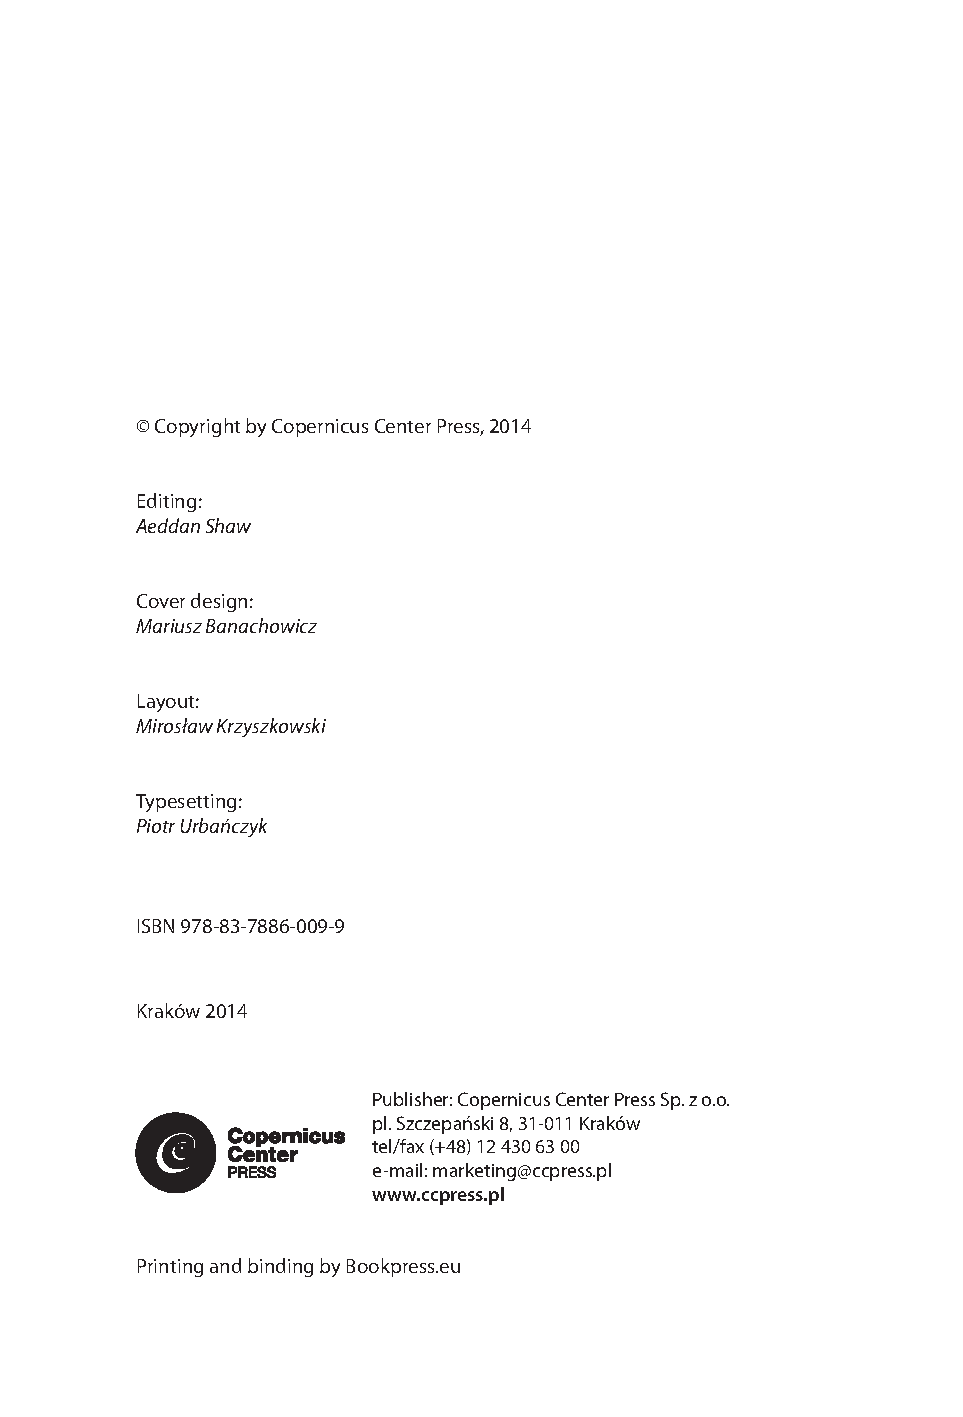
\includepdf[pages=1]{images/CT4.pdf}


\thispagestyle{empty}
\vspace*{1.2in}%
\begin{flushright}
\rectitle{Zagadnienia Filozoficzne\\w Nauce}\par
\vspace*{.5in}%
\chaptitleeng{Philosophical Problems\\in Science}\par
\end{flushright}
\vfill
\clearpage

\thispagestyle{empty}

\vfill

\noindent\begin{czw}© Copernicus Center Press, \rok\end{czw}

\vfill

\begin{adres}
	\begin{pagname}\noindent\begin{czwad}Editorial Board\end{czwad}\\
		Editor-in-Chief: dr hab. Paweł Jan Polak\\
		Deputy Editor-in-Chief: dr hab. Janusz Mączka\\
		Honorary Editor: prof. dr hab. Michał Heller\\
		Guest Editors: dr Bartłomiej Skowron, dr Michał Eckstein\\
		Editorial Secretary: Piotr Urbańczyk
		
	\end{pagname}
\end{adres}


\vfill


\noindent\begin{czw}Proofreading: dr Roman Krzanowski\end{czw}

\vskip.5em

\noindent\begin{czw}Adjustment and correction: Artur Figarski\end{czw}

\vskip.5em

\noindent\begin{czw}Cover design: Mariusz Banachowicz\end{czw}

\vskip.5em

\noindent\begin{czw}Technical editor: Artur Figarski\end{czw}

\vskip.5em

\noindent\begin{czw}Typographic design: Piotr Urbańczyk\end{czw}

\vskip.5em

\noindent\begin{czw}Typeset in \end{czw}\LaTeX

%\noindent\begin{czw}Skład: Artur Figarski\end{czw}


\vfill

\begin{adres}
	\begin{pagname}\noindent ISSN 0867-8286 (print format)\\
		e-ISSN 2451-0602 (electronic format)
	\end{pagname}
\end{adres}

\vfill

\begin{adres}
		\noindent\begin{czwad}Editorial Office\end{czwad}
	
		\noindent\begin{pagname}Zagadnienia Filozoficzne w Nauce
		
		\noindent Wydział Filozoficzny UPJPII
		
		\noindent ul. Kanonicza 9, 31-002 Kraków
		
		\noindent POLAND
		
		\vskip.3em
		
		\noindent e-mail: zagadnienia@upjp2.edu.pl
		
		\noindent www.zfn.edu.pl\end{pagname}
\end{adres}

\vfill

\begin{wrapfigure}{L}{.3\textwidth}
	\noindent\includegraphics[width=.29\textwidth]{images/ccp.pdf}
%\noindent\includegraphics[width=.27\textwidth]{images/ccp.pdf}
\end{wrapfigure}
\vskip.4em
%\noindent\parbox[t]{6cm}{
\begin{adres}
	\noindent\begin{pagname}Publisher: Copernicus Center Press Sp. z o.o.
		
		\noindent pl. Szczepański 8, 31-011 Kraków POLAND
		
		\noindent tel. (+48) 12 448 14 12
		
		\noindent e-mail: marketing@ccpress.pl
		
		\noindent www.ccpress.pl\\ \end{pagname}
	
	
\end{adres}
%}




\clearpage

%	\thispagestyle{empty}
	\begin{flushright}%
	{\bigtitle{Zagadinienia\\Filozoficzne\\w Nauce\par}}%
	\vspace{0.2in}%
	{\chaptitleeng{Philosophical Problems in Science\par}}%
	\vspace{0.2in}%
	\hrule%
	{\LARGE\textbf{{\numerrzymski -- \rok}}}%
	\hrule%
	\end{flushright}%
%		\@mkboth{\czwit\contentsname}{\czwit\contentsname}%
	\vspace{0.5in}%
%
%\clearpage

%Spis tresci -------------------------------------------------

{\thispagestyle{plain} \tableofcontents \clearpage}
%--------------------------------------------------------------------------------------------
\newpage
\thispagestyle{plain}
\cleardoublepage
\thispagestyle{plain}

%--------------------------------------






%\ramkaart{Imię Nazwisko}
{Tytuł rozdziału.\\\chapsubtit{Podtytuł rozdziału}}
{Tytuł rozdziału. Podtytuł rozdziału}
{Tytuł rozdziału. Podtytuł rozdziału}

\lettrine[loversize=0.13,lines=2,lraise=0.00,nindent=0em,findent=0.2pt]%
{W}{}ielu filozofów i językoznawców twierdziło, że gdy identyfikujemy przedmioty, zarówno w języku, jak i w postrzeganiu, kierujemy się względami praktycznymi, potrzebami, wolą -- krótko mówiąc, swego rodzaju interesem, czy to gatunkowym (a więc ogólnoludzkim), czy to swoistym dla danej społeczności, cywilizacji czy jednostki. Wydaje się to kłócić z przeświadczeniem, że te przedmioty muszą istnieć, chyba że traktujemy to przeświadczenie jako jedną z wielu równouprawnionych wizji świata. Ta sama zasada wielości równosilnych perspektyw stosuje się a fortiori do języka metafizyki.

Tak więc powracamy tam, gdzie nasz horror bierze swój początek. Jakże mam trwać przy danym języku (czy jakimś szczególnym punkcie widzenia, z którego patrzę na świat, albo regule interpretacji całości doświadczenia), nie przyznając mu uprzywilejowanej poznawczej mocy? A jeśli pretenduję do dysponowania wyższym czy może nawet absolutnym językiem, to albo nadawałby się on tylko do mówienia o innych językach, nie zaś o rzeczywistości, do której się odnoszą, albo byłby standardowym językiem, a inne byłyby jego niekompletnymi dialektami. W tym drugim przypadku byłby to rzeczywiście boski język, absolutny i zawierający wszelkie wyobrażalne punkty widzenia. Lecz język taki jest niemożliwy; nawet Bóg, przemawiając ustami proroka, musiał się przełożyć na język ludzki; przekład jest niechybnie zniekształcony, a nam brak dostępu do oryginału. W przypadku pierwszym język mój (język pierwszego stopnia, język rzeczy) nie może wprawdzie rościć sobie pretensji do jakiejkolwiek pozycji uprzywilejowanej, lecz w tym języku nie sposób byłoby nieobecność owej pozycji wyrazić: by to uczynić, musiałbym swój język porzucić i przejść do super(czy meta-) języka -- ale w takim języku moje stanowisko, jako że szczególne, nie dałoby się wyrazić.

\myquote{
Gdy więc wielkodusznie powiadam: „wszystkie stanowiska metafizyczne są równie dobre”, sam żadnego stanowiska nie zajmuję, po prostu wyrażam zasadę tolerancji, która, jakkolwiek chwalebna, ma charakter formalny i nigdy nie wyda, czy choćby zainspiruje, żadnej metafizycznej idei. Lecz próbując zachować tę zasadę i obstawać zarazem przy swym szczególnym punkcie widzenia, popadam w niekonsekwencję, jako że twierdzę wtedy, iż „stanowisko moje jest tak samo dobre jak każde inne, mimo że jest nie do pogodzenia z żadnym innym”.

A jeśli tak mówię, nie mogę w zrozumiały sposób wyjaśnić, w jakim sensie to stanowisko jest moje, w przeciwieństwie do innych. Niestety, tolerancyjna wspaniałomyślność nie pozwala uciec od paradoksu samoodniesienia.
}

\noindent Leon Chwistek, logik i malarz, w wydanej w 1921 roku książce Wielość rzeczywistości sugerował istnienie czterech rodzajów wzajemnie niezależnych (a zatem przypuszczalnie nieinterferujących z sobą wzajem) rzeczywistości: rzeczy, takie jak je postrzega zdrowy rozsądek; rzeczy nauk fizycznych; wrażeń; i wyobraźni. Znajdują one swój artystyczny wyraz w malarstwie – odpowiednio: prymitywistycznym, naturalistycznym, impresjonistycznym, futurystycznym\footnote{To jest przypis dolny. Jeśli niezależne od siebie pokłady rzeczywistości wymagają dla swego opisu niezależnych języków, sugeruje to, że języki te są całkowicie nieprzekładalne; skoro tak, to w istocie można sądzić, że różne wizje świata współistnieć mogą w doskonałej wzajemnej obojętności}. Lecz wielość ta, dowodził, pozwala na dowolną liczbę równoprawnych poglądów na świat, z których żadnego nie można dowieść, lecz każdy jest do przyjęcia pod warunkiem, że nie próbuje zmonopolizować prawdy. Dopuszczalne stają się różne odpowiedzi na tradycyjne pytania, jak te o wolność woli, relację między ciałem a duchem, obiektywność wartości, jeśli zakres odniesienia ogranicza się do jednej lub niektórych spośród owych czterech rzeczywistości.

\noindent Leon Chwistek, logik i malarz, w wydanej w 1921 roku książce Wielość rzeczywistości sugerował istnienie czterech rodzajów wzajemnie niezależnych (a zatem przypuszczalnie
nieinterferujących z sobą wzajem) rzeczywistości: rzeczy, takie jak je postrzega zdrowy rozsądek

\section{Podtytuł 1 stopnia}

\noindent Teoria wielu -- jakkolwiek wyodrębnianych -- rzeczywistości, jeśli nawet w tym przypadku stworzona dla metafizycznej interpretacji malarstwa, proponuje przekonujący i kuszący obraz świata. Jednakże jako propozycja epistemologiczna nie jest w stanie -- czy to w wersji Chwistka, czy Williama Jamesa -- poradzić sobie z wciąż tą samą trudnością: jak dowieść wyższości pewnej teorii bytu w tym samym języku, w którym została wypowiedziana? Mieliżbyśmy utrzymywać, że twierdzenie „wszystko jest konieczne” jest równie prawomocne co twierdzenie „poza związkami logicznymi nic nie jest konieczne” i że doktryna, według której słowo „ja” nie ma odniesienia, jest nie mniej prawdziwa niż ta, wedle której cokolwiek ma odniesienie, jest względne w stosunku do „ja”?

\subsection{Podtytuł 2 stopnia}

\noindent Jeśli niezależne od siebie pokłady rzeczywistości wymagają dla swego opisu niezależnych języków, sugeruje to, że języki te są całkowicie nieprzekładalne; skoro tak, to w istocie można sądzić, że różne wizje świata współistnieć mogą w doskonałej wzajemnej obojętności: nie mogą być ze sobą konfrontowane ani między sobą sprzeczne. Ale twierdzenie, że nie mogą być konfrontowane, jest wyrażone w języku innym, wyższego stopnia, nie nadającym się do celów metafizycznych. I tu powraca ten sam kłopot: albo ograniczamy się do tego wyższego języka i wtedy werdykty nasze nie mają znaczenia dla rzeczywistych problemów, z których filozofia żyje, albo przyjmujemy pewną metafizyczną perspektywę i głosimy, że perspektywy tej, jako zamkniętej, nie da się zharmonizować z żadną inną ani też innej przeciwstawić -- i wtedy też, w wyniku tej samointerpretacji, perspektywa nasza jest bez znaczenia dla rzeczywistych problemów, z których filozofia żyje.

\sectionno{Podtytuł 1 stopnia}

\noindent Teoria wielu -- jakkolwiek wyodrębnianych -- rzeczywistości, jeśli nawet w tym przypadku stworzona dla metafizycznej interpretacji malarstwa, proponuje przekonujący i kuszący obraz świata. Jednakże jako propozycja epistemologiczna nie jest w stanie -- czy to w wersji Chwistka, czy Williama Jamesa -- poradzić sobie z wciąż tą samą trudnością: jak dowieść wyższości pewnej teorii bytu w tym samym języku, w którym została wypowiedziana? Mieliżbyśmy utrzymywać, że twierdzenie „wszystko jest konieczne” jest równie prawomocne co twierdzenie „poza związkami logicznymi nic nie jest konieczne” i że doktryna, według której słowo „ja” nie ma odniesienia, jest nie mniej prawdziwa niż ta, wedle której cokolwiek ma odniesienie, jest względne w stosunku do „ja”?

\subsection{Podtytuł 2 stopnia}

\noindent Jeśli niezależne od siebie pokłady rzeczywistości wymagają dla swego opisu niezależnych języków, sugeruje to, że języki te są całkowicie nieprzekładalne; skoro tak, to w istocie można sądzić, że różne wizje świata współistnieć mogą w doskonałej wzajemnej obojętności: nie mogą być ze sobą konfrontowane ani między sobą sprzeczne. Ale twierdzenie, że nie mogą być konfrontowane, jest wyrażone w języku innym, wyższego stopnia, nie nadającym się do celów metafizycznych. I tu powraca ten sam kłopot: albo ograniczamy się do tego wyższego języka i wtedy werdykty nasze nie mają znaczenia dla rzeczywistych problemów, z których filozofia żyje, albo przyjmujemy pewną metafizyczną perspektywę i głosimy, że perspektywy tej, jako zamkniętej, nie da się zharmonizować z żadną inną ani też innej przeciwstawić -- i wtedy też, w wyniku tej samointerpretacji, perspektywa nasza jest bez znaczenia dla rzeczywistych problemów, z których filozofia żyje.

\section{Podtytuł 1 stopnia}

\noindent Teoria wielu -- jakkolwiek wyodrębnianych -- rzeczywistości, jeśli nawet w tym przypadku stworzona dla metafizycznej interpretacji malarstwa, proponuje przekonujący i kuszący obraz świata. Jednakże jako propozycja epistemologiczna nie jest w stanie -- czy to w wersji Chwistka, czy Williama Jamesa -- poradzić sobie z wciąż tą samą trudnością: jak dowieść wyższości pewnej teorii bytu w tym samym języku, w którym została wypowiedziana? Mieliżbyśmy utrzymywać, że twierdzenie „wszystko jest konieczne” jest równie prawomocne co twierdzenie „poza związkami logicznymi nic nie jest konieczne” i że doktryna, według której słowo „ja” nie ma odniesienia, jest nie mniej prawdziwa niż ta, wedle której cokolwiek ma odniesienie, jest względne w stosunku do „ja”?

\subsection{Podtytuł 2 stopnia}

\noindent Jeśli niezależne od siebie pokłady rzeczywistości wymagają dla swego opisu niezależnych języków, sugeruje to, że języki te są całkowicie nieprzekładalne; skoro tak, to w istocie można sądzić, że różne wizje świata współistnieć mogą w doskonałej wzajemnej obojętności: nie mogą być ze sobą konfrontowane ani między sobą sprzeczne. Ale twierdzenie, że nie mogą być konfrontowane, jest wyrażone w języku innym, wyższego stopnia, nie nadającym się do celów metafizycznych. I tu powraca ten sam kłopot: albo ograniczamy się do tego wyższego języka i wtedy werdykty nasze nie mają znaczenia dla rzeczywistych problemów, z których filozofia żyje, albo przyjmujemy pewną metafizyczną perspektywę i głosimy, że perspektywy tej, jako zamkniętej, nie da się zharmonizować z żadną inną ani też innej przeciwstawić -- i wtedy też, w wyniku tej samointerpretacji, perspektywa nasza jest bez znaczenia dla rzeczywistych problemów, z których filozofia żyje.

\begin{thebibliography}{00}{Imię Nazwisko}
{Tytuł rozdziału. Podtytuł rozdziału}

\makeatletter
    \clubpenalty10000
    \@clubpenalty \clubpenalty
    \widowpenalty10000
\makeatother


\bibitem{Abc}
A.~Abc, \textit{Abc}...

\bibitem{Xyz}
A.~Abc, \textit{Abc}...

\end{thebibliography}





%\sekcja{Od Redakcji}{Editorial}

%\input{EDI_Kwarcinski/Kwarcinski.tex}



\sekcja{Artykuły}{Articles}

\begin{artengenv}{Colin McLarty}
	{Mathematics as a love of wisdom: Saunders Mac~Lane as philosopher}
	{Mathematics as a love of wisdom: Saunders Mac~Lane as philosopher}
	{Mathematics as a love of wisdom: Saunders Mac~Lane\\as philosopher}
	{Department of Philosophy, Case Western Reserve University}
	{This note describes Saunders Mac Lane as a philosopher, and indeed as a paragon naturalist philosopher. He approaches philosophy as a mathematician.  But, more than that, he learned philosophy from David Hilbert's lectures on it, and by discussing it with Hermann Weyl, as much as he did by studying it with the mathematically informed Göttingen Philosophy professor Moritz Geiger.}
	{naturalism, philosophy, mathematics, Aristotle.}


\vspace{3ex}
\begin{flushright}
  Go, read, and disagree for yourself.\\\parencite[p.~390]{MacLBell46}
\end{flushright}\vspace{3ex}

\lettrine[loversize=0.13,lines=2,lraise=-0.03,nindent=0em,findent=0.2pt]%
{T}{}his note describes Saunders Mac~Lane as a philosopher, and indeed as a paragon naturalist philosopher. Obviously he approaches questions in philosophy the way a mathematician would.  He is one.  But, more deeply, he learned philosophy by attending David Hilbert's public lectures on it, and by discussing it with Hermann Weyl, as much as he did by studying for a qualifying exam on it with the mathematically informed G\"ottingen Philosophy professor Moritz Geiger \parencite{McLSaundersLast,McLSaundersReck}.\footnote{Mac~Lane's close contact with Paul Bernays in G\"ottingen deserves more attention.  But my research so far has not identified strong philosophic influence from Bernays.  See Section~\ref{S:Learning}.}  Before comparing Mac~Lane to Penelope Maddy's created naturalist, the Second Philosopher, we relate him as a philosopher to Aristotle.


This is not to disagree with Skowron's view of Mac~Lane as a platonist in ontology \parencite{SkowTalk}.  This is about Mac~Lane on scientific and philosophic method.  He understood \textit{philosophy} very much as Aristotle did: Philosophy is the love of wisdom, and every science pursues wisdom and not mere facts.  I do not claim Mac~Lane got the ideas from Aristotle.  So far as I know, Mac~Lane himself had no interest in or opinion of Aristotle, though his teachers Weyl and Geiger certainly talked of Aristotle.\footnote{\textcite{BrowderMacL} give a beautiful survey of mathematics which mentions Plato and Aristotle on ontology.  However, the discussion of Plato and Aristotle summarizes the longer discussion by \textcite{BrowderRel}.}





\section{Aristotle on wisdom and science}\label{S:Aristotle}
\myquote{
  In general the sign of knowing or not knowing is the ability to teach, so we hold that art rather than experience is scientific knowledge;  some can teach, some cannot. Further, the senses are not taken to be wisdom.  They are indeed the authority for acquaintance with all individual things, but they do not tell the why of anything, for example why fire is hot, but only that it is hot.\\
  \indent It is generally assumed that what is called wisdom is concerned with the primary causes and principles, so that, as has been already stated, those who have experience are held to be wiser than those who merely have any kind of sensation, the artisan than those of experience, the craft master than the artisan.  (Aristotle, Metaphysics 981f.)\footnote{Translations of Aristotle here use ``know'' for \textit{oida}, ``scientific knowledge'' for \textit{episteme}, and ``acquaintance'' for \textit{gnosis}.  Of course ``wisdom'' is \textit{sophia}.}
}

Here Aristotle says scientific knowledge is better than acquaintance, or even experience, in two related ways:
\begin{enumerate}
  \item scientific knowledge can be taught, and
  \item scientific knowledge gives the why of things.
\end{enumerate}
He says wisdom deals with primary causes and principles.  And those are his touchstone for scientific knowledge: ``We do not know or have scientific knowledge of objects of any methodical inquiry, in a subject that has principles, causes, or elements, until we are acquainted with those and reach the simplest elements'' (Physics 184a).

Throughout his career Mac~Lane tied pedagogy to research and research to craft.  Among many examples see his early notes on presenting mathematical logic to university students \parencite{MacLSymbolic}, and his impassioned argument that theoretical education prepared men and women well to do the applied mathematics which he supervised in World War~II \parencite{MacLColumb,MacLReq}.

Mac~Lane also insists mathematical understanding includes knowing the reasons for a given theorem.  Some proofs of a theorem may reveal the reason, while other technically sufficient proofs will not reveal the reason. In his book for philosophers, Mac~Lane sketches proofs for major theorems from many subjects, like linear algebra, or complex analysis.  He often describes several alternative proofs for a single theorem and then eventually singles out one as giving the real reason.  That book is \parencite{MFF} and some examples are on pages 145, 189, 427, 455.

For me, though, the deepest connection between Aristotle's and Mac~Lane's loves of wisdom is how they say we gain this scientific knowledge.  Both believe in foundations, or ``first principles'' if you prefer, but neither believes we start with those. Aristotle's theoretical demand of philosophy was a theoretical and practical demand in mathematics for Mac~Lane:

\myquote{
The natural way of [getting scientific knowledge] is to start from the things which are more knowable and obvious to us and proceed towards those which are clearer and more knowable by nature; for the same things are not 'knowable relatively to us' and 'knowable' without qualification. So in the present inquiry we must follow this method and advance from what is more obscure by nature, but clearer to us, towards what is more clear and more knowable by nature. (Physics 184a)
}

Aristotle speaks of advancing from what is initially clear to us, towards what is more knowable by nature.  I am not sure if he believed there was a final point where the absolutely first principles and simplest elements are known so that they will never change.  Mac~Lane certainly did not believe it for mathematics.

From his early work on field theory \parencite{MacSchZero,MacSchNorm} and for the rest of his career Mac~Lane often worked to find more basic concepts in some part of mathematics. He and Eilenberg spent over a decade collaborating on ever broader uses of the concepts in their ``General theory of natural equivalences'' \parencite{GenTh}.  They meant that paper to be the only one ever needed on this technical concept for group theory and topology, but it became the founding paper of the whole field of category theory.

Only in the 1960s, after meeting graduate student Bill Lawvere, did Mac~Lane come to believe category theory could be a foundation for all mathematics.  Even then, precisely because of all the concrete mathematics that had gone into developing his ideas, Mac~Lane insisted this, and any foundation for mathematics, must be seen as ``proposals for the organization of mathematics'' \parencite[p.~406]{MFF}.  The optimal organization (i.e.~the optimal foundation) will change as mathematics develops, and will help advance those developments.  He warned that excessive faith in any ``fixed foundation would preclude the novelty which might result from the discovery of new form'' \parencite[p.~455]{MFF}.


\section{Mathematics as a love of wisdom}

Let us come to cases with one paradigmatically philosophical question, and one paradigmatically mathematical.  For Mac~Lane these questions are inseparable:%\vspace{2ex}
\begin{itemize}
         \item[Q$_1$] What are mathematical objects, and how do we come to know them? %\vspace{1ex}
         \item[Q$_2$] What are solutions to a Partial Differential Equation (PDE), and how do we come to know them?
       \end{itemize}
For Mac~Lane Q$_2$ can only be a specific case of Q$_1$.  For him, as for Aristotle, basic questions of the special sciences \textit{are} philosophy.  They cannot \textit{not} be philosophy.

Let us be clear:  A mathematician can learn a textbook answer to Q$_2$ without ever asking for a philosophy behind it.  In just the same way, a philosopher can learn the currently received answers to Q$_1$ from philosophy books, without ever asking about live mathematics.  Admittedly the math textbook answers will be more stable over time than the philosophically received answers. But that is not important.  For Mac~Lane, both of those ways of learning are failures of understanding.  They are failures of \textit{philosophy}.  For him, an answer to either one of those questions can only be valuable to the extent that you can see what it is \textit{good for}---for Mac~Lane that cannot be either a purely technical mathematical question or a purely academic philosophic one.  Think back to his work in World War II.

Mathematicians speak of solutions to PDEs in many ways:
\begin{itemize}
  \item Smooth (or, sufficiently differentiable) function solutions.
  \item Symbolic solutions.
  \item Generalized function solutions (of various kinds\dots).
  \item Numerical solutions\dots.
\end{itemize}
These different senses of solutions are sought in very different ways.  There are well understood relations between them, but the relations are not all obvious and in particular cases they may be quite difficult, and important, to find.

Mac~Lane's war work certainly involved relating different kinds of solutions to PDEs.  Even when an equation has a known exact solution by an easily specified smooth function, applying it also requires numerical solutions.  The worker has to choose which aspects are best handled in theory, so as to direct and optimize the calculations, and when best to leave theory and begin calculating.  Those choices are rarely textbook work. They are often not clear cut at all.  They require exactly what Aristotle called the wisdom of the craft master. Namely, they require grasping the \textit{why} of each kind of solution.  They require knowing not only the technical definition of each kind of solution, but \textit{what good} each one is, and especially \textit{the good} of their relations to one another.

The craft master, having wisdom, knows the whys, can teach them, and supervise work with them.

As I write this, I imagine some practice-minded philosopher challenging: ``How are philosophies like logicism, formalism, and intuitionism going to help anyone solve or apply a PDE?'' Indeed. This is why Mac~Lane so often deprecates those philosophies.  But just to give one example, Mac~Lane argued that formalism in Hilbert's hands was a step towards programmable computers. See Section~\ref{S:Learning}.  Those unquestionably help solve PDEs.

\section{The philosophy of mathematicians\\in 1930s G\"ottingen}\label{S:Learning}

\myquote{
\textit{Wir d\"urfen nicht denen glauben, die heute mit philosophischer Miene und \"uberlegenem Tone den Kulturuntergang prophezeien und sich in dem Ignorabimus gefallen. F\"ur uns gibt es kein Ignorabimus, und meiner Meinung nach auch f\"ur die Naturwissenschaft \"uberhaupt nicht. Statt des t\"orichten Ignorabimus heiße im Gegenteil unsere Losung:
Wir m\"ussen wissen -- wir werden wissen!}%\vspace{2ex}


We must not believe those, who today, with philosophical bearing and deliberative tone, prophesy the fall of culture and accept the ignorabimus. For us there is no ignorabimus, and in my opinion none whatever in natural science. In opposition to the foolish ignorabimus our slogan shall be:
We must know -- we will know!  \parencite[p.~385]{HilbNaturerkennen}\footnote{Before we try to defend or defeat Hilbert's slogan as an assertion in academic epistemology, it is in fact the most important statement in philosophy of mathematics of the past 150 years. I use the translation by \textcite[p.~1164]{ewald2005kant}.  Hilbert's address was  broadcast on the radio and a recording is available at  \url{math.sfsu.edu/smith/Documents/HilbertRadio/HilbertRadio.mp3}.}
}
Hilbert's conclusion, \textit{Wir m\"ussen wissen -- wir werden wissen!}, is engraved on his tomb in G\"ottingen.


Mac~Lane arrived in G\"ottingen just at the time Hilbert was promoting this slogan.  I do not recall Mac~Lane quoting it in lectures or conversations.  He did not have to quote Hilbert.  Everything Mac~Lane said illustrated this faith.  As you can see in \textcite{MFF,MacLAuto}, or \textcite{McLSaundersLast}, Mac~Lane followed Hilbert's mathematizing scientific optimism, rather than the specific finitist program (often called ``formalism,'' though not by Hilbert) of Hilbert's famous \textit{On the Infinite}~\parencite*{HilbUnend}.  Mac~Lane did see specific, productive mathematical value in that program though, and rejected a criticism of it by Freeman Dyson~\parencite{MacLDyson}.

Dyson supposed Hilbert seriously meant to reduce all mathematics to formal reasoning, and said ``the great mathematician David Hilbert, after thirty years of high creative achievement[\dots]\ walked into a blind alley of reductionism.''  Specifically, Dyson claimed that Hlbert ``dreamed of'' formalizing all mathematics, solving the decision problem for this formal logic, and ``thereby solving as corollaries all the famous unsolved problems of mathematics.''  Mac~Lane replied:
\myquote{I was a student of Mathematical logic in G\"ottingen in 1931-1933, just after the publication of the famous 1931 paper by G\"odel. Hence I venture to reply [\dots].
Hilbert himself called this `metamathematics.' He used this for a specific limited purpose, to show mathematics consistent. Without this reduction, no G\"odel's theorem, no definition of computability, no Turing machine, and hence no computers [\dots]. Dyson simply does not understand reductionism and the deep purposes it can serve.
}

Mac~Lane gives a concise expert review of these issues and places them in the context he knew at the time they arose.  He insists Hilbert did not tie the slogan ``we must know, we will know'' to the decision problem.  Rather, Mac~Lane says, ``[Hilbert] held that the problems of mathematics can all ultimately be solved'' without supposing metamathematics will do it. Full disclosure: I admit that after long consideration, drawing on \textcite{SiegProg,SiegBook}, I myself am unsure exactly how Hilbert and/or Bernays intended their work on the decision problem at various times. But however that may be, Mac~Lane understood Hilbert this way.  And this is Mac~Lane's own far from reductionist faith, while recognizing reductionist methods for what they actually have achieved in mathematics.

Mac~Lane learned a lot in frequent discussions with Bernays.  But for now I have to say I see no larger trace of those discussions in Mac~Lane's philosophy than is found in the letter on Dyson.  Mac~Lane's book on philosophy of mathematics is titled \textit{Mathematics: Form and Function}.  But this is clearly ``form'' as Mac~Lane learned about it from talking with Weyl and studying under Geiger~\parencite{McLSaundersLast}. It does not refer to formalism in any sense related to Bernays.  Or, at least, so it seems to me.  The reader is encouraged to go, read, and disagree if they see something else.



\section{Naturalism}\label{S:naturalism}

The decisive feature marking Penelope Maddy's Second Philosopher as a \textit{naturalist} is that:

\myquote{[She] sees fit to adjudicate the methodological questions of mathematics---what makes for a good definition, an
acceptable axiom, a dependable proof technique?---by assessing the effectiveness of the method at issue as means towards the
goals of the particular stretch of mathematics involved. \parencite[p.~359]{MadSecBook}
}
Lots of mathematicians, and essentially all leading mathematicians, do the same.\footnote{If by axioms Maddy means specifically axioms of set theory then few mathematicians ever learn those, let alone adjudicate them. Mac~Lane is famously among those few.}

The unusual thing about Mac~Lane in this regard is that he was explicitly tasked by the US government to evaluate mathematics research and teaching methods in classified reports during World War II and publicly after that.\footnote{See \textcite{MacLFederal,MacLColumb,MacLChina} and \textcite{SteingartPhD}.}  Those reports were explicitly directed to various different specific short-term and long-term goals.  All the variety he saw, and dealt with, left Mac~Lane ever more deeply impressed with the actual unity of the whole.


Precisely that background, along with his experience as Chair of the Chicago Mathematics Department, made Mac~Lane diverge from another feature of Maddy's Second Philosopher:
\myquote{
All the Second Philosopher's impulses are methodological, just the thing to generate good science [\dots].~\cite[p. 98]{MadSecond}
}
All Mac~Lane's impulses aim at producing good science and for this reason they  are not \textit{all} methodological.

Mac~Lane, like Aristotle, knows methods alone generate no science.  Besides evaluating methods of reaching goals, at least some mathematicians must evaluate goals. For Aristotle, those should be the craft masters, the wise.  In his vivid words: ``the wise should not accept orders but give them;  nor should they be persuaded, but the less wise should''~(Metaphysics 982a).  We will see, though, Mac~Lane is less focused on command than that.  He inclines more to another passage: ``those who are more accurate and more able to teach about the causes are the wiser in each branch of knowledge'' (Metaphysics 982a).


Because of his broad experience, especially evaluating both methods and goals for mathematics, Mac~Lane cannot agree that ``the goal of philosophy of mathematics is to account for mathematics as it is practiced, not to recommend reform.'' \parencite[p.~161]{MadNat} %([1997].  
Just sticking to the mathematician philosophers we have already named: Hilbert, Weyl, and Mac~Lane all knew reform is integral to mathematical practice.  You cannot separate reform from practice if you try.  And all three made explicitly philosophic arguments for their recommended reforms along with more technically mathematical ones.\footnote{Hilbert had sweeping success with his reforms.  Among many philosophic works by and on  him see~\textcite{HilbLogGrund,HilbNaturerkennen}. \textcite{WeylKontinuum} advocated what Weyl took to be Brouwer's philosophy, while \textcite{WeylDer,WeylOf} trace his eventual, regretful conclusion that in fact Hilbert was right about this and Brouwer wrong.}   This is important for philosophy of mathematics.

The paradigm case for anti-revisionism in philosophy of mathematics is Brouwer's intuitionism.  Brouwer is by far the favorite illustration of a revisionist, and is the sole example that the \textit{Stanford Encyclopedia of Philosophy} discusses under anti-revisionism in the article ``Naturalism in the Philosophy of Mathematics'' \parencite{SEPnaturalism}:
\myquote{
The mathematician-philosopher L.E.J. Brouwer developed intuitionistic mathematics, which sought to overthrow and replace standard (‘classical’) mathematics.
}

So it is important for philosophers to understand that the problem with Brouwer, according to all our exemplars Hilbert, Weyl, and Mac~Lane, is not that he had philosophical motives.  It is that he was wrong.  Actually, for Mac~Lane, Brouwer's philosophy was at best wrong.  At worst it was ``pontifical and obscure'' \parencite{MacLSymbolic}.

Immediately upon completing his doctorate in mathematics at G\"ot\-tin\-gen, Mac~Lane put a philosophy article in  \textit{The Monist}~\parencite{MacLMonist}.  Fifty years later he wrote a book describing, as he told me, what he wanted philosophers to know about math~\parencite{MFF}.  There he asks about the large array of mathematics he surveyed:
``How does it illuminate the philosophical questions as to
Mathematical truth and beauty and does it help to make judgements
about the direction of Mathematical research?''  \parencite[p.~409]{MFF}
There is a reason he puts these questions together.

He asks about mathematical truth and beauty knowing very well that few mathematicians want to pursue the question seriously, and knowing philosophers who speak of it rarely know much of the wealth.  For Mac~Lane both of those are failures of understanding and they are nothing he means to promote.\footnote{À propos, I consider Edna St.~Vincent Millay's poem ``Euclid alone has looked on Beauty bare'' incredibly true to its topic, despite that she apparently studied no mathematics beyond school textbooks based on bits of Euclid's \textit{Elements}.}  He means to promote mathematically informed philosophic pursuit of the question of mathematical truth and beauty.  And so he does of the question on the direction of research.  He seriously means to promote philosophic thought on that.  Of course he does not see philosophic thought as the sole preserve of those with philosophy degrees.  No more does he see philosophy of math as the sole preserve of those with math degrees.   Mathematics for Mac~Lane, when pursued with full awareness of its worth, is philosophy.

\end{artengenv}


\begin{artengenv}{Zbigniew Semadeni}
	{Creating new concepts in mathematics: 
	  freedom and limitations.
	  The case of\\Category Theory}
	{Creating new concepts in mathematics: 
		  freedom and limitations\ldots}
	{Creating new concepts in mathematics: 
		  freedom and limitations.\\
		  The case of Category Theory}
	{Institute of Mathematics, 
	  University of Warsaw}
	{The purpose of the paper is to discuss the problem of possible limitations 
	of freedom in mathematics and to look for criteria which would help us 
	to distinguish---in the historical development of mathematics---new concepts 
	which were natural follow-ups of the previous ones from new concepts which opened 
	unexpected ways of thought and reasoning. \par
	The rise of category theory (CT) is analysed, in particular, earlier ideas (which 
	were precursors of the theory) and its initial development. The question of the 
	the origin of the term \textit{functor} is discussed; the presented evidence strongly 
	suggests that Eilenberg and Carnap could have learned the term from Kotarbi{\'n}ski 
	and Tarski.}
	{categories, functors, Eilenberg-Mac Lane Program, mathematical 
	cognitive transgressions, phylogeny, platonism.}








\section{Introduction}
\lettrine[loversize=0.13,lines=2,lraise=-0.03,nindent=0em,findent=0.2pt]%
{T}{}he celebrated dictum of Georg Cantor that ``The very essence of mathematics lies 
precisely in its freedom'' expressed the idea that in mathematics one can freely 
introduce new notions (which may, however, be abandoned if found unfruitful or 
inconvenient).\footnote{The italics in the original sentence ``Das \textit{Wesen 
der Mathematik} liegt gerade in ihrer \textit{Freiheit}'' are Cantor's. 
The first version was published in 1879, reprinted in \parencite[p.34]{Cantor}, discussed 
by \citeauthor{Ferreiros} \parencite*[p.257]{Ferreiros}. } %%% koniec footnote
This way Cantor declared his opposition to claims of Leopold Kronecker who objected 
to the free introduction of new notions (particularly those related to the infinite). 

Some years earlier Richard Dedekind stated that---by forming, in his theory, a cut 
for an irrational number---we \textit{create} a new number. For him this was an example 
of a constructed notion which was a free creation of the human mind \parencite[\S~4]{Stetigkeit}. 

In 1910 Jan Łukasiewicz distinguished \textit{constructive notions} from empirical 
\textit{reconstructive} ones. He referred (with reservation) to Dedekind’s statement 
and pointed out that a consequence of our ``creation'' of those notions is the 
 spontaneous emergence of countless relations which no more depend on our will. 

Until the discovery of non-Euclidean geometries, geometry was regarded as an 
abstraction of the spatial reality. The freedom of creation in geometry was 
limited by this reality. Hilbert advocated a formal point of view, broadening the 
freedom of choosing the axioms, while Poincar\'e maintained that the axioms of 
geometry are conventions.
 
Clearly, the freedom of mathematics is limited by logical constraints. At the same 
time, logical inference yields deep meaning to mathematics. As Michał Heller put it, 
``If I accept one sentence, I must also accept another sentence. Why must I? 
Who forces me? 
Nobody. Yet, I must. Generally, we bear badly any restrictions of our liberty, but 
in the case of mathematical deduction inevitability of the conclusion gives us the 
feeling of safety (I have not deviated from the way) and of the accompanying 
intellectual comfort, sometimes even great joy'' \parencite[p.21]{Heller}. 

A mathematician trying to prove a theorem knows the feeling of an invisible wall 
which blocks some intended arguments. Also new concepts must be consistent with 
earlier ones and must not lead to contradiction or ambiguity. Moreover, in 
mathematical practice, only intersubjective mental constructions are accepted.  

The purpose of this paper\footnote{The present paper is based on a talk delivered 
at XXIII Kraków Methodological Conference 2019: {\it Is Logic a Physical Variable?}, 
7-9 November 2019.} % koniec footnote
is to look for restraints and patterns in the historical development of 
mathematics.\footnote{ The significant question of degree of freedom in mathematical 
conceptualization of physical reality is not considered here.}  % koniec footnote
Some types of paths will be distinguished, first generally, in the context of 
the historical development of mathematics, and then they will be used to highlight 
some features of the rise of category theory (CT). 

Michael Atiyah, in his \textit{Fields Lecture} at the World Mathematical Year 2000 
in Toronto, expressed his view that ``it is very hard to put oneself back in 
the position of what it was like in 1900 to be a mathematician, because so much 
of the mathematics of the last century has been absorbed by our culture, by us. 
It is very hard to imagine a time when people did not think in those terms. In fact, 
if you make a really important discovery in mathematics, you will then get omitted 
altogether! You simply get absorbed into the background'' \parencite[p.1]{Atiyah}. 

This statement may be appear startling, as the mathematical meaning of a text from 
around 1900 is generally believed to be time-proof. Yet what Atiyah had in mind was 
not the meaning of published texts---definitions, theorems and proofs---
but the way mathematicians thought at that time. 

It was 75 years ago when the celebrated paper by 
%Samuel Eilenberg and Saunders Mac Lane 
\citeauthor{E-ML} was published.\footnote{Mac Lane earlier in his life (in particular 
in \parencite{E-ML} and \parencite{Duality} wrote his name as MacLane. Later he 
began inserting a space into his surname, in particular in \parencite{Working}. } 
This event marked the rise of category theory (CT). As the 
development of mathematics accelerated in the second half of the 20\textsuperscript{th} century, 
it may be hard to fully imagine how mathematicians thought in 1945. Their 
definitions, theorems and comments are clear, but one should be aware that a 
reconstruction of their ideas, their thinking may be specifically biased by our 
present understanding of the mathematical concepts involved. 

\section{Background conceptions}
The main ideas of this paper---which includes a very wide spectrum 
of examples, from ancient Greek mathematics to modern, from children’s counting 
to CT---are the following: 
\begin{itemize} 
\item A mathematical concept, no matter how novel, is never independent of the 
previous knowledge; it is based on a reorganization of existing ideas. 
\item A radically new mathematical idea never germinate in somebody's mind 
without a period of incubation, usually a lengthy one. 
\item There is a long distance to cover between: \par 
(1) a spontaneous, unconscious use of a mathematical idea or structure in a concrete 
setting, \par 
(2) a conscious, systematic use of it. 
\item A person who has achieved a higher level of mathematical thinking is often 
unable to imagine thinking of a person from another epoch or of a present learner 
and, consequently, may unconsciously attribute to him/her an inappropriate (to high 
or too low) level of thinking.  
\end{itemize}

\subsection{Transgressions}
A \textit{mathematical cognitive transgression} (or briefly: a \textit{transgression}) 
is defined as crossing---by an individual or by a scientific community---of 
a previously non-traversable limit of own mathematical knowledge or 
of a previous barrier of deep-rooted convictions. Moreover, it is assumed that: \par
\begin{enumerate} 
\item the crossing concerns a (broadly understood) mathematical idea and the difficulty 
is inherent in the idea, 
\item the crossing is critical to the development of the idea and related 
concepts, 
\item it is a passage from a specified lower level to a new specified upper level, 
\item the crossing is a result of conscious activity (the activity need not 
be intentional and purposely orientated towards such crossing; generally such 
effect is not anticipated in advance and may even be a surprise). 
\end{enumerate} 

In the history of mathematics there were numerous transgressions, of different 
importance, some great ones and many ``mini-transgressions''. Usually they were 
not single acts---they involved a global change of thinking which matured for 
years or even generations and they based on the work of many people. In ancient 
times two transgressions were the most significant: 
\begin{itemize}
\item The transition from practical dealing with specific geometric shapes to deductive 
geometry.  
\item The celebrated discovery (in the 5\textsuperscript{th} century BC) that the diagonal of a 
square is incommensurable with its side, that they are 
\textgreek{'alogos} 
(\textit{a-logos}), without a ratio, irrational (in modern setting, foreign to Greek 
thinking, it was the irrationality of $\sqrt{2}$) \cite[pp.80-81]{Baszmakowa}. 
The Pythagorean paradigm was undermined by this \textgreek{apor'ia}.
Their understanding of mathematics was eroded. However, nothing certain is 
known about this discovery. Stories presented in popular books are based on 
doubtful legends from sources written seven or eight centuries later 
\parencite[p.21, 51]{Knorr}. This incommensurability could not be a single 
discovery by an individual. It must have been a lengthy process. Never in the 
historical development of mathematics such a major change occurred in short time. 
\end{itemize}

\noindent In modern history there were many transgressions. Let us list some of 
the best known: 

\begin{itemize}
\item Acceptance of negative numbers.
\item The transition from potential infinity (infinity at a \textit{process} 
level) to the \textit{actual} infinity (infinity as an object). 
\item The emergence of projective geometry.  
\item The discovery of non-Euclidean geometries. 
\end{itemize}

\noindent We will discuss the case of CT, arguing in particular that creating the 
theory of \textit{elementary topoi} in CT should be regarded as a major transgression. 

\subsection{Phylogeny and ontogeny}
The term \textit{phylogeny} refers here to the evolutionary history of mathematics 
(or rather to its modern reconstructions), from ancient times on. 
\textit{Ontogeny} means the development of basic mathematical concepts and 
structures in the mind of an individual person, from early childhood. Phylogeny and 
ontogeny are in some sense complementary descriptions \parencites[][]{HF}[][pp.4-29]{P-G}.
%% Freudenthal, Piaget-Garcia 

In case of mathematics, the oft-quoted phrase: \textit{ontogeny recapitulates 
phylogeny} implies that one can learn from the history of old mathematics for the 
sake of present teaching. This sometimes gives useful hints, e.g. one may argue that 
since the historical process of forming the general concept of a function took 
centuries (from Descartes, if not much earlier, to Peano and Hausdorff), we should 
not expect that a secondary school student can grasp it---learning Dirichlet’s 
description---after a few lessons. The general concept of the function was not 
yet quite clear to mathematicians of the first half of the 19\textsuperscript{th} century 
\parencites[][Appendix 2]{Lakatos}{Youschkevitsch}[][pp.27--30]{Ferreiros}. 

On the other hand, the idea that ontogeny recapitulates phylogeny may be misleading. 
Piaget always stressed that arithmetic cognition results from logico-mathematical 
experience with concrete objects, pebbles say, and is educed from \textit{the 
child’s actions} rather than from heard words. It is abstracted from a coordination of 
intentional motions and accompanying thoughts. Nevertheless, Piaget was in favour 
of the phylogeny-ontogeny parallelism and reasoned roughly as follows. Since 
one-to-one correspondence preceded numerical verbal counting in the very early 
periods of human civilization (evidenced on artefacts such as notched bones and 
also found in rude unlettered tribes), the same should apply to children. Cantor’s 
theory of cardinal numbers confirmed this thinking \parencite[pp.259--260]{B-P}.
Consequently, Piaget and many educators insisted on one-to-one correspondence 
as a foundation of early school arithmetic, neglecting the fact that nowadays 
children learn number names early, often together with learning to speak, and 
moreover counting is now deeply rooted culturally. Research evidence shows that 
counting, rather than one-to-one correspondence, is a basis of the child’s 
concept of number \parencite[pp.77--82]{G-G}.
In this way the phylogeny–ontogeny parallelism adversely affected early mathematics 
education in the time of the `New Math' movement. 

Hans Freudenthal, in the context of mathematics, suggested the converse idea: 
\textit{What can we learn from educating the youth for understanding the past of 
mankind?} \,This reverses the traditional direction of inference in the 
phylogeny–ontogeny parallelism. In particular, one may ask whether contemporary 
knowledge of the difficulties in the transition from the concrete to more abstract 
mathematical reasoning of children may be helpful in better understanding of 
limitations of our reconstructions of the development of the early Greek mathematics.  

In the sequel, certain aspects of the development will be traced both in phylogeny 
and in ontogeny, inextricably % [nierozdzielnie] 
intertwined with the the mathematical questions themselves. 

\subsection{Platonizing constructivism in mathematics}
The theoretical framework of the paper is platonizing constructivism in mathematics. 
It is assumed that: 
\begin{itemize} 
\item each of the three major positions in the philosophy of mathematics from the beginning of 
the 20th century: \textit{platonism}, \textit{constructivism}, \textit{formalism} 
describes some inherent, complementary features of mathematics; 
\item they can be reconciled provided that they are regarded as \textit{descriptive}, 
as an account of some inherent features of mathematics, and \textit{not normative}, 
i.e., when one skips the eliminating words (as `only', `oppose') which explicitly deny 
other standpoints. Moreover, various versions of the three positions often overlap. 
\end{itemize}

\noindent In the sequel, the term \textit{constructivism} will not be understood as in papers on 
foundations of mathematics, but rather in a way akin to its meaning in research on mathematics 
education, related to post-Piagetian psychological versions of constructivism. 
Briefly, one assumes here that humans construct mathematical concepts in their minds  
and discover their properties. A~concept develops its necessary structure 
as a consequence of its context and---in the long term---becomes 
\textit{cristalline} in the sense of David \citeauthor{Tall} \parencite*[p.27]{Tall}; then its 
properties appear independent of our will. 
This phenomenon may be traced both in phylogeny and in ontogeny. 
Moreover, in each essential progression, new mental structures are build on the 
preceding ones and are always integrated with previous ones \parencite[pp.22--29]{P-G}.  

By platonizing constructivism we mean an analysis---in constructivistic terms 
--- of sources and consequences of the platonistic attitude of a majority of 
mathematicians and contrasting them with the well-known difficulties of consistent 
platonism in the philosophy of mathematics. 

\section{Developmental successors}
After the introductory examples we now look for ways to distinguish between: 
\begin{itemize}
\item mathematical concepts which---historically---were natural successors to 
previous ones,  
\item concepts which could be conceived and defined only 
after opening new paths of thought and reasoning. 
\end{itemize}

\noindent The following metaphorical labels will be used: \textit{onward development}, 
\textit{branching-off},    %%% \textit{merging}, 
\textit{upward development}, \textit{downward development}, interpreted with 
examples. We do not expect to find clear criteria, but the ensuing discussion 
may be illuminating. 

The \textit{emergence of numerals} in the Late Stone Age is evidenced by tally 
marks (in the form of notched bones). Ethnologists have found that early tribes 
had only two counting words: \textit{one} and \textit{two}, followed by \textit{many}. 
Also in present Indo-European languages these two numbers and their ordinal 
counterparts are linguistically different from the following numbers. 
It has been suggested that the proto-Indo-European number *\textit{trei} (three) was 
derived from the verb *\textit{terh} (meaning: \textit{pass}); thus, the word 
\textit{three} is related to \textit{trans}. This may be a hint of a very ancient 
mental obstacle between numbers \textit{two} and \textit{three}. 

One may conjecture that \textit{after the passage from 2 to 3 there was no notable 
obstacle to gradual development of unlimited counting}. Of course, the actual 
development took centuries, if not millennia. Anyway, for present children 
there is no hurdle between 2 and 3, as they are taught counting very early. 
Moreover, counting starts to make sense with three items. 

\subsection{Onward development}
Onward development of indefinite counting includes its \textit{developmental 
successors}: simple addition of natural numbers (which develops through a stage 
called \textit{count all} and then a more advanced stage \textit{count on}), 
subtraction (as taking away), multiplication, division (originally there are two 
kinds of it: \textit{equal sharing} and \textit{equal grouping}), and even simple 
powers, all within some range of natural numbers.  

These concepts are included in the onward development of counting, by virtue of 
the following features: 

\begin{itemize}
\item \textit{no branching}: each new concept naturally comes after the previous ones; 
\item \textit{ontological stability}: each concept (e.g., number 17, product 
\mbox{$3\times 6$}), remains essentially the same object, although the related 
ideas are enriched after each extension of the scope of arithmetic and---in the 
historical development---are subject to evolutionary changes.
\end{itemize}

The conception of developmental successors, outlined here, does not take into account 
a relative difficulty of concepts; what is crucial is whether they follow the previous 
lines of thinking. 

\subsection{Branching-off}
This conception arises from a negation of the first requirement in the description 
of an onward development. An example of it are fractions, which \textit{branch off} 
from natural numbers; it is not onward development, although there are many ties 
between natural numbers and fractions. 

There are two ways of introducing fractions to children. In the first, some 
idealized whole is divided into $m$ equal parts and then $n$ of them are taken. 
In the second, $n$ whole things are equally divided into $m$ parts. 
They are two main aspects of the concept of a fraction. For instance, $\frac{3}{4}$ 
of pizza may be obtained by cutting it into 4 parts and taking 3 such parts 
(thus $\frac{3}{4} = 3 \times \frac{1}{4}$). A more advanced way of thinking of 
$\frac{3}{4}$ is 3 divided by 4; the latter may be explained with the example 
of 3 pizzas to be divided among 4 persons. 

The distinction looks quite elementary. Yet, it was significant in the phylogeny 
of fractions. First procedure is akin to that of ancient Egyptians, the 
second -- to Greek ratios; both were inherited by Arabic mathematicians. In the 
ontogeny the two ways are always present, but not necessarily noticed. The 
following reminiscence by William Thurston (1946-2012), written 8 years after 
he had received Fields Medal, describes his discovery of the identification of 
previously different objects. 

\myquote{
I remember as a child, in fifth grade, coming to the amazing (to me) realization 
that the answer to 134 divided by 29 is $134/29$ (and so forth). What a tremendous 
labor-saving device! To me, `134 divided by 29' meant a certain tedious chore, 
while $134/29$ was an object with no implicit work. I went excitedly to my father 
to explain my major discovery. He told me that of course this is so, $a/b$ and 
$a$ divided by $b$ are just synonyms. To him it was just a small variation in 
notation \parencite[p.848]{Thurston}.
}

\noindent The fraction $\frac{a}{b}$ becomes identified with the result of division 
$a\div b$ and---in this synthesis---they both form a single mathematical object. 
Philosophically, however, it is an ontological change: two different beings, results 
of two different mental constructions, become regarded as a single one. 

Onward branching-off can be traced in many parts of mathematics.  
Calculus branches off from a theory of the field of real numbers (axiomatic or 
based on a construction). 
Infinite sequences of real numbers branch off from elementary algebra of real numbers. 
Limits of sequences branch off from general theory of sequences. 
These examples vividly show that the question of distinguishing branching-off from 
onward development is delicate, as the criteria are far from being precise, but it 
may contribute to better understanding the historical development of mathematics. 

\subsection{Upward development and downward development}
By \textit{upward development} of a piece of mathematics we mean passing from some 
concepts and relations between them to a more abstract version of them. Examples: 
\begin{itemize}
\item Transition from practical addition (verbalized as, e.g., \textit{two and 
three make five}) to symbolic version (e.g., 2+3=5) took centuries (the sign $+$ 
appeared in some 15\textsuperscript{th} century records; the first occurrence of the equality 
sign $=$ was found in a text by a Welsh mathematician Robert Recorde from 1557). 
\item Transition from $\mathbb{R}^n$ 
to an axiomatically given vector space over $\mathbb{R}$.  
\item Transition from a vector space over $\mathbb{R}$ 
to a vector space over a field. 
\item Transition from group theory to the category \textbf{Grp}. 
\item Transition from a category to a metacategory (in the sense 
of \parencite[pp.7--11]{Working}). 
\end{itemize}

\textit{Downward development} is---in some sense---an inverse process, 
to more concrete questions or to a lower level of abstraction, so the above examples 
may be used the other way round. Also some typical applications of mathematics 
may be included here, e.g., the passage from abstract Boolean algebras to a 
description of certain types of electrical circuits (as conceived by Claude \citeauthor{Shannon_symbolic_1936}~\parencite*{Shannon_symbolic_1936}).

In the 20\textsuperscript{th} century the mathematics grew rapidly and the upward development became 
much easier mentally as a result of both: a general change of the attitude of 
mathematicians toward abstraction and the routine of expressing all concepts in 
the language of set theory. 
Branching-off were so frequent that the above metaphors are of little use. 
There is, however, a notable exception: a new theory which opened a new direction 
of thinking, so its beginnings may be discussed in a way akin to that used with 
respect to distant past.   

\section{The rise of category theory (CT)}
A very special feature of CT is that it has a pretty precise date of its official 
birth: the publication of the paper by Samuel Eilenberg and Saunders Mac Lane 
\parencite*{E-ML}. It was presented at a meeting of the American Mathematical Society in 
1942 and published in 1945.

According to the Stanford Encyclopedia of Philosophy, \textit{CT ``appeared almost out 
of nowhere''}. Not quite so. As in any mathematical theory, some CT ideas had been 
conceived much earlier, particularly in algebraic topology, and some of them can 
be traced to the 19\textsuperscript{th} century. 

Many conceptual transformations---either explicit and well recognized or 
used implicitly, without awareness---contributed to the rise of CT. Going back,  
a significant factor was the historic development of the mathematical concept of 
a function. 

Until the beginning of the 19\textsuperscript{th} century, a general symbol for a function ($f$ or 
$\varphi$) was almost non-existent \parencite{Youschkevitsch}. 
A significant step toward CT was the general notion of a mapping introduced by 
Dedekind in 1888. In his \textit{Enkl{\"a}rung} (\textit{explanation}) 
he did not define the concept of \textit{Abbildung} $\varphi$ (literally: 
\textit{image} or \textit{representation}) from a set (\textit{System}) $S$ into a set 
$S^\prime$, but interpreted it generally as an arbitrary law (\textit{Gesetz}) according 
to which to each element $s$ there corresponds (\textit{geh{\"o}rt}) a certain 
thing (\textit{Ding}) $S^\prime = \varphi(s)$, called the image (\textit{Bild}) 
of~$s$. He also defined a composed mapping (\textit{zusammengesetzte Abbildung}) 
$\vartheta(s) = \psi(s^\prime) = \psi(\varphi(s))$ of two given ones, denoted 
as $\varphi.\psi$ or $\varphi\psi$, defined injective mappings (\textit{{\"a}hnlich} 
or \textit{deutlich}), the inverse mapping and proved their main properties 
\parencites[][\S2--4]{Was_sind}[][p.88--90, 228--229]{Ferreiros}.

Emmy Noether in her lectures in the 1920s emphasised the role of homomorphisms 
in group theory. Before her, groups were understood as generators and relations 
(in modern terms, as quotients of free groups). She also argued that the homology 
of a space is a group, is an algebraic system rather than a set of numbers assigned 
to the space. Her lectures and the lectures of Emil Artin formed a basis for the 
celebrated book by van der Waerden \parencite*{Waerden} on modern algebra. This current 
of thought led to CT.

Generally, in the symbol of the type $f(x)$, the part $f$ was always understood 
as fixed and $x$ was a variable. At the end of the 1920s, however, in functional 
analysis and related fields, a new way of thinking emerged. In certain situations 
the roles of symbols in $f(x)$ reversed: the point $x$ was regarded as fixed while 
the function $f$ became a variable (as an element of a function space), e.g., 
$x\in [0,1]$ was fixed and $f$ was a variable in the space $C([0,1])$ of continuous 
functions on the interval $[0,1]$. In this new role, the point $x$ became a functional 
$\delta_x$ on $C([0,1])$. Such a change of the roles function-element became crucial, 
e.g., in the Potryagin duality of locally compact abelian groups \parencite{Hewitt} 
and in Gelfand’s theory of commutative Banach algebras. It was also used by \citeauthor{E-ML} 
in their first example (finite dimensional vector spaces 
and their dual spaces) motivating the concept of a natural equivalence.  

A crucial example of a contravariant functor was the adjoint $T^\ast$ of a linear 
operator $T$ on a Hilbert space, introduced in 1932 by John von Neumann.\footnote{\citeauthor[p.330]{Century} tells a story how Marshall Stone advised von Neumann to introduce the symbol $T^\ast$ and how it changed the publication. He also 
mentions a fact which may interests philosophers: in 1929 von Neumann lectured in 
G{\"o}ttingen and presented his axiomatic definition of a Hilbert space, while David 
Hilbert---listening to it---evidently thought of it as of the concrete 
space $\ell^2$, not in the axiomatic setting.} % koniec footnote

According to Mac Lane, abstract algebra, lattice theory and universal algebra were 
necessary precursors for CT. However, he also suggested that certain notational 
devices preceded the definition of a category. One of them was the fundamental idea 
of representing a function by an arrow $f\colon X\to Y$, which first appeared in 
algebraic topology about 1940, probably introduced by Polish-born topologist Witold 
Hurewicz \parencites[][p.29]{Working}[][p.333]{Century}. Originally, it looked as just 
another symbol, but from a later perspective the use of such symbol was one of the 
key changes. Thus, a notation (the arrow) led to a concept (category). Such new symbols 
later got absorbed into the background of mathematical thinking, used as something 
obvious. Together with commutative diagrams, which were probably also first used by 
Hurewicz, they paved the way to CT. 

Mac Lane often accented two features of mathematics: computational and conceptual. 
He noted that the initial discovery of CT came directly from a problem of calculation 
in algebraic topology \parencite[p.333]{Century}.

Eilenberg and Mac Lane were aware that they introduced very abstract mathematical 
tools, which did not fit any algebraic system in the Garrett Birkhoff's universal 
algebra. It might seem too abstract and was certainly off beat and a ``far out'' 
endeavour. Although it was carefully prepared, it might not have 
seen the light of day \parencite[p.130]{MLonE}.

\subsection{The origin of the term \textit{functor} }
Mac Lane has written ``\textit{Categories, functors, and natural transformations 
were discovered by Eilenberg–Mac Lane in 1942}'' \parencite[p.29]{Working}. The word 
``discovered'' may be regarded as an indication of a hidden Platonistic attitude 
of Mac Lane, in spite of his verbal declarations against
Platonism \parencites[][pp.447--449]{Form}[][]{Krol}[][]{Skowron}. He also wrote: 

\myquote{
  Now the discovery of ideas as general as these is chiefly the willingness to 
  make a brash or speculative abstraction, in this case supported by the pleasure 
  of purloining words from the philosophers: ``Category'' from Aristotle and Kant, 
  ``Functor'' from Carnap (\textit{Logische Syntax der Sprache}) 
  \parencite[pp.29--30]{Working}.
}

\noindent This sentence has been taken very seriously by several authors. However, 
the way it was phrased suggests that it was rather intended to be a delicate 
joke.\footnote{ Let us note that the noun \textit{brash} means a mass of fragments; 
according to \textit{Cambridge International Dictionary of English} (1995), the 
adjective \textit{brash} is disapproving, referring to people who show too much 
confidence and too little respect, while \textit{Webster's New World Dictionary} 
(1984) lists---as meanings of \textit{brash}---also \textit{hasty and reckless}, 
\textit{offensively bold}. On the other hand, the word \textit{purloining} means 
\textit{stealing} or \textit{borrowing without permission}. Such a comment (with 
the word \textit{pleasure}) by Mac Lane concerning CT could not be serious. On the 
other hand, in 2002 Mac Lane came back to Carnap, adding: 
``Also the terminology was largely purloined: “category” from Kant, “natural” 
from vector spaces and “functor” from Carnap. (It was used in a different sense in 
Carnap’s influential book \textit{Logical Syntax of Language}; I had reviewed the English 
translation of the book (in the Bulletin AMS 1938) and had spotted some errors; 
since Carnap never acknowledged my finding, I did not mind using his 
terminology)'' % end quote ital.
\parencite[pp.130--131]{MLonE}.} % end of footnote
Attributing the origin of the term \textit{category} to Aristotle and Kant is clear, 
although in 1899 Ren\'e-Louis Baire (in his \textit{Th\`ese}) introduced---in 
another context---the word \textit{category} to 
mathematics.\footnote{ A subset $A$ of a topological space $X$ is called \textit{a 
set of first category} (\textit{un ensemble de pre\-mi\`ere cat\'e\-gorie}) in $X$ 
iff $A$ is the union of a countable family of nowhere dense sets; otherwise it is 
\textit{a set of the second category} (\textit{Menge erster und zweiter Kategorie}). 
The celebrated \textit{Baire category theorem} states, in a generalized form, 
that a complete metric space is not a set 
of the first category \parencites[][p.328]{Hausdorff}[][\S~10]{Kuratowski}. The 
clumsy term \textit{set of the first category} was later replaced by the term 
a~\textit{meager set} \parencite[p.201]{Kelley}. In the 1930s Baire category theorem 
was a very popular tool in the Warsaw school of topology, so Eilenberg must have 
known it.} % end of footnote
Concerning the origin of the term \textit{functor} in CT, one may recall the 
following facts:\footnote{ The author is indebted to Professor Jan Wole\'nski 
for the relevant information.} 

\begin{itemize}
\item In Rudolf Carnap's book \textit{Abriss der Logistik} \parencite{Abriss} the term ``Funktor'' does not appear. 
\item In 1929 the Polish term ``funktor'' was used in propositional calculus by 
Tadeusz Kotarbi\'nski in his book \parencite{Kotarbinski}.
\item Alfred Tarski often emphasised that Kotarbi\'nski had been his teacher 
\parencite[part~2]{Feferman}. 
\item Carnap met Tarski in Vienna in February 1930 and visited Warsaw in November 
1930; he learned much from Tarski. 
\item In 1933 Tarski, in the Polish version of his famous paper \textit{On the 
concept of truth in formal languages} \citeauthor{Tarski} \parencite*{Tarski} used the term ``funktor'' 
and mentioned that he owed the term to Kotarbiński.  
\item Carnap used the term ``Funktor''  in his book \parencite*{Logische} (quoted 
by Mac Lane) in a sense more general than that of Kotarbi\'nski and Tarski. 
\item Eilenberg studied mathematics in Warsaw from 1930. In 1931 he attended 
Tarski's lectures on logic \parencite[part~3 and~12]{Feferman}. He left Warsaw in 1939. 
\end{itemize}

This evidence strongly suggests that both Carnap and Eilenberg could have learned, 
independently, the term from Kotarbi{\'n}ski and Tarski.

\subsection{Was the original CT an onward development of previous mathematical theories?}
Using a metaphor explained above, one may argue that the definition of a 
category and of a functor were within a major onward development of part of 
mathematics of the first half of the 20th century, that is set theory, 
algebra, topology etc. Indeed, for a person working in group theory, say, 
a natural continuation should be to think of all groups, their homomorphisms, 
isomorphisms, and the composites as of a single whole: \textit{group theory}. 
Similarly one could think of vector spaces with linear maps as of another whole. 
Some analogies between theories were obvious. Moreover, axioms of CT are 
reminiscent of those of semigroup theory. The concept of a covariant functor 
was a natural analogue of homomorphisms of algebras. Contravariant functors 
had been present in various duality theories (e.g., in Pontryagin’s duality 
mentioned above). CT provided general concepts applicable to all branches of abstract 
mathematics, contributed to the trend towards uniform treatment of different 
mathematical disciplines, provided opportunities for the comparison of 
constructions and of isomorphisms occurring in different branches of mathematics, 
and may occasionally  suggest new results by analogy \parencite[p.236]{E-ML}. 

The great achievement of Eilenberg and Mac Lane was the idea that a formalization of 
various evident analogies was worth systematizing and publishing. The initial neglect 
of \parencite{E-ML} by mathematicians was very likely a result of the fact that it was 
regarded as a long paper within onward development of known part of mathematics, with 
many rather simple definitions and examples, tedious verification of easy facts, 
and no theorem with an involved proof. Ralf Kr{\"o}mer, in his book on the history 
and philosophy of CT, has outright stated that Eilenberg and Mac Lane needed to 
have remarkable courage to write and submit for publication the paper almost 
completely concerned with conceptual clarification \parencite[p.65]{Kromer}. 

A novelty of \parencite[p.272]{E-ML}, which at first appeared insignificant, was regarding 
elements $p_1, p_2$ of a single quasi-ordered set $P$ as objects of a category, 
with a unique morphism $p_1 \to p_2$ iff $p_1 \le p_2$ and no morphisms otherwise. 
This opened a way to a series of generalizations, in particular regarding certain 
commutative diagrams as functors on small categories. 

One may argue that this achievement was still within onward development of CT 
as it was within the scope of previous knowledge. Let us recall that the 
difficulty and the originality of a theorem are not taken into account; what is 
crucial is whether the concepts involved are natural extension of the previous 
knowledge and thinking. 

The category axioms represent a very weak abstraction \parencite[p.25]{Goldblatt}. 
In spite of this fact, a few years later the conceptual clarification turned out 
highly effective in the book \textit{Foundations of Algebraic Topology} written 
by Eilenberg together with Norman Steenrod \parencite*{Steenrod}. The latter admitted in a 
conversation that the 1945 paper on categories had a more significant impact on 
him than any other research paper, it changed his way of thinking. 

\subsection{The Eilenberg-Mac Lane Program}
This program has been formulated as follows: 
\myquote{
The theory also emphasizes that, whenever new abstract objects are 
constructed in a specified way out of given ones, it is advisable to regard 
the construction of the corresponding induced mappings on these new objects 
as an integral part of their definition. The pursuit of this program entails 
a simultaneous consideration of objects and their mappings (in our terminology, 
this means the consideration not of individual objects but of categories). [...] 
\par The invariant character of a mathematical discipline can be formulated in 
these terms. Thus, in group theory all the basic constructions can be regarded 
as the definitions of co- or contravariant functors, so we may formulate the 
dictum: The subject of group theory is essentially the study of those constructions 
of groups which behave in a covariant or contravariant manner under induced 
homomorphisms. More precisely, group theory studies functors defined on well 
specified categories of groups, with values in another such category. This may be 
regarded s a continuation of the Klein Erlanger Programm, in the sense that a 
geometrical space with its group of transformations is generalized to a category 
with its algebra of mappings. \par 
[...] such examples as the ``category of \textit{all} sets'', the ``category of 
\textit{all} groups are illegitimate. The difficulties and antinomies are exactly 
those of ordinary intuitive \textit{Mengenlehre}; no essentially new paradoxes are 
involved. [...] we have chosen to adopt the intuitive standpoint, leaving the reader 
free to insert whatever type of logical foundation (or absence thereof) he may prefer. 
[...] \par It should be observed first that the whole concept of a category is 
essentially an auxiliary one; our basic concepts are essentially those of a functor 
and of a natural transformation. [...] The idea of a category is required only by the 
precept that every function should have a definite class as domain and a definite 
class as range, for the categories are provided as the domains and ranges of functors.
\parencite[p.236--237, 246--247]{E-ML}
}

The quoted comparison of CT to the celebrated program of Felix Klein shows vividly 
that the authors regarded their work as significant. 
A important novelty of \parencite{E-ML} was to use the same letter to denote both: 
the object component of a functor and its morphism component. This had not been 
a common practice, even when both correspondences were dealt with in a single 
paper. This novelty and the whole program fit well Atiyah's conception (quoted 
above) of ideas \textit{absorbed by mathematicians' culture}. 

CT is both a specific domain of mathematics and at the same time a conceptual framework 
for a major part of modern theories. 

\section{The amazing phenomenon of unexpected branchings-off in CT}
Up to this point CT might be regarded are being within onward development of 
earlier theories: algebra, topology, functional analysis. However, a~branching-off 
in \parencite{E-ML} is the concept of a \textit{natural equivalence} (central in the title 
of the paper), with an essential use of commutative diagrams.\footnote{ It is not 
clear why Eilenberg and Mac Lane refrained from setting the concept in the general 
form of a \textit{natural transformation} (examples abounded). Perhaps they felt 
they should not pursue a still more general setting without accompanying 
results.} % end of footnote
It was a completely new idea, but its initial impact was limited. 

After 1945 CT---as a general theory---lay dormant till the emergence of 
significant new concepts and a breaking series of major branchings-off in the 
second half of the 1950s. One of their outstanding features was a new type of a 
definition, formulated in the form of a \textit{unique factorization problem}. 
First such explicit definition \parencite*{Samuel} appeared in the paper by Pierre Samuel, 
a member of the Bourbaki group, on free topological groups, albeit it was still 
in the language of set theory, without arrows. 
In \cite*{Duality}, commutative diagrams were demonstrated as a convenient 
tool in such problems by  \citeauthor{Duality}. 
The concept of a \textit{dual category}, formulated in \parencite[p.259]{E-ML} and 
further developed by \citeauthor{Duality} \parencite*{Duality}, had its conceptual roots in various 
duality theories, particularly in that of projective geometry. The \textit{product} 
of two categories was an analogue of that for groups and various algebras. 
Mac Lane analysed the concept of duality, 
stressed diagrammatic dualities of various pairs of concepts and presented the 
definitions of \textit{direct} and \textit{free products} in group theory (later 
generalized to the concepts of categorial \textit{products} and \textit{coproducts}, 
respectively). 

\subsection{A metamorphosis from Eilenberg--Mac Lane Program to mature CT}
A turning point in the development of CT was the seminal paper by Daniel \citeauthor{Kan} \parencite*{Kan}
on \textit{adjoint functors}. In much the same time period, independently, 
several closely related concepts and results were worked out: \textit{representable 
functors}, \textit{universal morphisms}, \textit{Yoneda lemma}, various types of 
\textit{limits} and \textit{colimits} \parencite[pp.345--352]{Century}. Special cases of 
them had a long earlier history in specific situations in algebra and topology 
(e.g., Freudenthal's theorems on \textit{loops} and \textit{suspensions} in homotopy 
theory proved in 1937). This confirms a known phenomenon that mathematicians may use 
an idea spontaneously, without being conscious of it in a more abstract setting. 

\citeauthor{Duality} \parencite*{Duality} also opened the way to the study of categories with additional 
structure, which some years later developed to the study of abelian categories. This 
topic was developed---in a remarkably short time---due to the work of Alexandre 
Grothendieck, David Buchsbaum, Pierre Gabriel, Max Kelly and authors of two 
monographs: Peter  \citeauthor{Freyd} \parencite*{Freyd} and Barry \citeauthor{Mitchell} \parencite*{Mitchell}. 

Within 20 years CT, originally conceived as a useful language for mathematicians, 
became a developed, mature theory, something totally unexpected by its founders. 

\subsection{Set theory without elements} 
The results of the work of William Lawvere turned out to be not only a new branch of 
CT, but also opened new perspectives in mathematics, logic, foundations of mathematics, 
and philosophy. In his Ph.D.\ thesis at Columbia University in New York, 
supervised by Eilenberg (defended in 1963, known from various copies, with full 
text published 40 years later) many new ideas were presented, including a 
categorical approach to algebraic theories \parencite{Law-Semant}. 

Lawvere also tackled the general question as to what conditions a category 
must satisfy in order to be equivalent to the category \textbf{Set}. The idea looked 
analogous to the so-called \textit{representation theorems}, i.e., propositions 
asserting that any model of the axioms for a certain abstract structure must be 
(in some prescribed sense) isomorphic to a specific type of models of the theory 
or to one particular concrete model.\footnote{The oldest theorems of this type 
are: Cayley's theorem that every (abstract) group is isomorphic to a group of 
bijections of a set; Kuratowski's theorem that every partially ordered set is  
order-isomorphic to a family of subsets of a set, ordered by inclusion; theorem that 
every group with one free generator is isomorphic to $\mathbb{Z}$. 
Analogous examples are known in many theories.} % end footnote 
However, Lawvere's case was unique and controversial in the sense that his `sets' 
were conceived \textit{without elements}. The theory did not have the primitive 
notion ``element of''. And it did work. 

Specifically, Lawvere characterized \textbf{Set} (up to \textit{equivalence} of 
categories) as a category $\mathcal{C}$ with the following: an \textit{initial} 
object \textbf{0}; a \textit{terminal} object \textbf{1} (which gives rise to 
\textit{elements} of $A$ defined as morphisms from \textbf{1} to $A$); 
\textit{products} and \textit{coproducts} of finite families of objects; 
\textit{equalizers} and \textit{coequalizers}; for any two objects there is an 
\textit{exponential}; existence of a specific object \textbf{N} with morphisms 
$0\colon \mathbf{1} \to \mathbf{N}$ and $s\colon \mathbf{N}\to \mathbf{N}$ yielding 
the successor operation $s$ on $\mathbf{N}$ and a simple recursion for sequences; 
axiom that \textbf{1} is a \textit{generator} (if parallel morphisms $f, g$ are not 
equal, then there is an element $x\in A$ such that $xf\ne xg$); axiom of choice; 
three additional elementary axioms of this sort (everything in the language of CT). 
This was augmented with one non-elementary axiom: $\mathcal{C}$ has products and 
coproducts for any \textit{indexing infinite set}. A coproduct of copies of 
\textbf{1} played the role of a set \parencites[]{Law-Sets}[][pp.386--407]{Form}[][pp.341--345]{Century}.  

The point was not to avoid membership relation completely, but (instead of 
taking as the starting point the primitive notions of \textit{set}, 
\textit{element} and membership $\in $) one takes \textit{function} as a primitive 
notion of the theory (with suitable axioms, using elementary logic, but avoiding any 
reference to sets) and then one derives membership and most concepts of set theory 
as a special case from there. 

In the second half of the 1960's Lawvere opened a way to a new theory of \textit{elementary 
toposes} (called also \textit{elementary topoi}, with Greek plural 
$\tau{\acute{o}}\pi o\iota$ of the noun $\tau{\acute{o}}\pi o\varsigma$). 
Unexpected territories of mathematics were discovered \parencites[][]{Law-Toposes}[][pp.352--359]{Century}[][]{Kromer}. 

CT became a contender for a foundation of mathematics, although the hope that it 
undermine the overwhelming role of set theory turned out spurious and most 
working mathematicians keep away from CT and toposes. CT yields new tools to study 
many formal mathematical theories and mutual relations between them, from a 
perspective different from that set theory.  

\section{Recapitulation of some points}  
Let us recall Atiyah's remark (quoted in the Introduction) that really important 
discoveries get later omitted altogether as they become absorbed by the general 
mathematical culture. This thought fits particularly well with the case of CT. Most 
of the ideas presented by Eilenberg and Mac Lane in 1945 have been absorbed as a 
natural language of advanced mathematical thinking. Once mathematicians learnt the 
definitions of a functor and a natural transformation, these concepts became a 
major tool of mathematical thinking in many abstract theories of the second half 
of the 20th century. However, it took several years to realise the scope of the 
change. Freyd commented as follows: 

\myquote{
MacLane's definition of ``product'' \parencite*{Duality} as the solution of a universal 
mapping problem was revolutionary. So revolutionary that it was not immediately 
absorbed even by most category minded people. \par 
[...] In a new subject it is often very difficult to decide what is trivial, 
what is obvious, what is hard, what is worth bragging about \parencite[p.156]{Freyd}. 
}

\noindent Mac Lane, however, used the definition of a product and its dual only in 
the case of groups (general or abelian). He did not formulate it \textit{mutatis 
mutandis} in the general case of a category, although he had several simple examples 
at hand. 
Freyd also told the story of the term \textit{exact sequence}, a technical 
definition in homological algebra. In the late 1950's, when he was a graduate student 
at Brown University, he was brought up to think in terms of exactness of maps. 
This concept seemed to him as fundamental as the notion of continuity must seem 
to an analyst. And later he was astonished to hear that when Eilenberg and  
Steenrod wrote their fundamental book \parencite{Steenrod} (published in 1952) they 
defined this very notion, recognized the importance of the choice of a suitable 
name for it, and could not invent any satisfactory word. Consequently, they 
wrote the word ``blank'' throughout most of the manuscript, ready to replace it 
before submitting the book for publication. After entertaining an unrecorded number 
of possibilities they settled on ``exact'' \parencite[p.157]{Freyd}. 

One may argue that the 1945 definitions of a category and of a functor were within a 
major onward development of abstract algebra and other advanced topics. In fact, 
originally they were not regarded as a novelty. Eilenberg and Mac Lane were not even 
certain whether their paper will be accepted for publication (it was long and lacked 
theorems with substantial proofs). However, they were genuinely convinced of the 
significance of their conceptual clarification and took pains to write the paper 
clearly and to attract the reader. 

After this publication for almost ten years CT appeared dormant. The groundbreaking 
papers on abelian categories by Buchsbaum and Gro\-then\-dieck marked 
a far-reaching change. And then---in the 1960's---CT unexpectedly started to 
grow rapidly, with astonishing results \parencite[pp.338--339, 341--361]{Century}.

Thus, from the present perspective, in spite of the previous arguments, one can say 
that the emergence of CT was undoubtedly a major transgression in mathematics. 
It was a crossing of a previously non-traversable barrier of deep-rooted habits to 
think of mathematics. A vivid argument is the fact that---even after publication 
of the main ideas---it was so difficult to overcome the previous inhibition 
and widespread tradition.\footnote{Many mathematicians, in USA and elsewhere, 
expressed disinclination to CT. Karol Borsuk, an outstanding topologist, the 
teacher of Eilenberg in Warsaw and coauthor of their joint paper published in 1936, 
was later unfavourable to CT and the categorical methods in mathematics 
\parencite[p.30]{Jackowski}. Jerzy Dydak, a student of Borsuk, recalled after years: 
\textit{My own PhD thesis written under Borsuk in 1975 makes extensive use 
of category theory and I was asked by him to cut that stuff out. Only after 
I assured him that I spent many months trying to avoid abstract concepts, he 
relinquished and the thesis was unchanged} \parencite[p.92]{Dydak}. } % end footnote

The creators of CT and their followers could choose their definitions freely, nobody 
could forbid that. And yet the previous way of thinking was an obstacle for 
potential authors and for prospective readers. Great insight of Eilenberg and 
Mac Lane of what is significant in mathematics turned out a crucial factor.  



\end{artengenv}

\begin{artengenv}{Jean-Pierre Marquis}
	{Abstract logical structuralism\edtfootnote{The author gratefully acknowledges the financial support of the SSHRC of Canada while this work was done. I also want to thank the organizers of the 23\textsuperscript{rd} Kraków Methodological Conference for inviting me and giving me the opportunity to give a talk in such a lovely venue.}}
	{Abstract logical structuralism}
	{Abstract logical structuralism}
	{Department of Philosophy, University of Montreal}
	{Structuralism has recently moved center stage in philosophy of mathematics. One of the issues discussed is the underlying logic of mathematical structuralism. In this paper, I want to look at the dual question, namely the underlying structures of logic. Indeed, from a mathematical structuralist standpoint, it makes perfect sense to try to identify the abstract structures underlying logic. We claim that one answer to this question is provided by categorical logic. In fact, we claim that the latter can be seen---and probably should be seen---as being a structuralist approach to logic and it is from this angle that categorical logic is best understood.}
	{philosophy, logic, structuralism, categorical logic.}





\section{Introduction}
\lettrine[loversize=0.13,lines=2,lraise=-0.03,nindent=0em,findent=0.2pt]%
{I}{}n their recent booklet \emph{Mathematical Structuralism}, \citeauthor{HellmanShap2019} \parencite*{HellmanShap2019}, %Hellman \& Shapiro 
give a list of eight criteria to evaluate various strands of mathematical structuralism. The very first criterion is the background logic used to express the version of structuralism examined: is it first-order, second-order, higher-order, modal? The claim made by Hellman \& Shapiro is that the logic has a direct impact on the philosophical thesis: for instance, the existence of non-standard models in first-order logic seems to affect some of the claims made by a mathematical structuralist. Be that as it may, it is assumed that any variant of mathematical structuralism is based on an underlying logic and the chances are that a change of logic will modify the type of structuralism defended. One then has to weigh the pros and the cons of adopting a specific logic to defend a kind of mathematical structuralism. 

This is all well and good, and I don't intend to discuss this assumption in this paper. Let me rather turn the question of the underlying logic on its head. A mathematical structuralist not only believes that \emph{pure} mathematics is about abstract structures, but also that \emph{pure} logic can be seen that way. In other words, a mathematical structuralist aspires to know what are the abstract structures underlying a given logic. Can logic itself  be given a structuralist treatment? In other words, is it possible to identify the \emph{abstract mathematical structures} from which the standard logical systems can be derived? In the same way that the natural numbers or the real numbers can be seen as specific structures arising from the combination of particular structures and properties, specific logical systems, e.g. intuitionistic first-order logic, classical first-order logic would result from the combination of particular abstract structures and properties. And important logical theorems---completeness theorems, incompleteness theorems, definability, undecidability, etc.---would be instances of abstract structural features, together with, presumably, singular properties. 

Our main claim in this paper is that categorical logic is one way to give precise answers to these questions.\footnote{In his \parencite*{Awodey1996}, often quoted as representing the categorical perspective on mathematical structuralism, Awodey did include a presentation of the basic features of logic from a categorical point of view, more specifically the internal logic of a topos. Given how he treated logic in his paper, none of his critics saw that he was including logic itself as an object of mathematical structuralism  \parencite[see, for instance,][]{Hellman2001,Hellman2003}. We approach the issues from a different angle.} Indeed, this is what categorical logic is all about: it reveals the abstract mathematical structures of logic and it relates them to other abstract mathematical structures, revealing yet other structural features. It also shows how the main results of logic are a combination of abstract structural facts and specific properties of logical systems. It is in this sense that one can say that \emph{pure} category theory \emph{is} logic.\footnote{Which is not to say that it is \emph{all} of logic. That is \emph{not} the claim.} This is one of the main \emph{points} of categorical logic. Thus, when mathematical structuralism is developed within the metamathematical framework of category theory, it is possible to give a positive answer to our new challenge. And as far as I know, it is at the time the only metamathematical framework that allows us to do it in such generality.

Of course, we are not claiming that the abstract analysis is \emph{superior} in a strong sense to the other presentations of logical systems. It brings a certain perspective, a certain understanding and opens up certain connections that are otherwise unavailable. Furthermore, in as much as a logic is applied, be it in foundational studies or in computer science, one also wants to look at it from a different point of view. But it has to be perfectly clear that these are completely different issues. We are now positioning ourselves in a structuralist framework, and will therefore ignore the aspects of a logic that become prevalent when one look at it for its applications. Ours is a \emph{philosophical} goal, not a technical one.


It goes without saying that categorical logic, seen as a search for the abstract structures of logic, did not come out of the blue. It was part of a larger mathematical movement, namely the structuralist movement in mathematics, which culminated in Bourbaki's \emph{Éléments de mathématique} \parencite[for more on the prehistory and the history of mathematical structuralism, see][]{Corry2004, Reck:2020}. It will therefore be worth our while to look briefly at the birth of categorical logic in the 1960s and early 1970s. We will merely indicate the major landmarks of the story, to see how indeed categorical logic was, right from the start, understood as being a part of that movement. We will then briefly look at some of the basic abstract structures that correspond to logic and then how some of the main theorems follow from features of abstract structures. At this point, to call the latter `mathematical' or `logical' is a matter of choice.

In the end, this paper should be taken as a challenge. We claim that one should add a ninth criterion of Hellman \& Shapiro's list: how does a given form of structuralism treat logic itself? Does it reveal the structures of logic? Are these structures related to other mathematical structures in a natural manner? Are these structures on the same level as the other fundamental structures of mathematics? One could, and we suggest that one should, evaluate different forms of mathematical structuralism according to this criterion. 

\section{The abstract structures of logic:\\setting the stage}

Although category, functors and natural transformations were introduced explicitly  in \cite*{EilMac1945} by \citeauthor{EilMac1945}, category \emph{theory} came to maturity only fifteen years later, thus at the beginning of the 1960s  \parencite[for more on this history, see, for instance][]{LandryMarquis2005,Kromer2007,Marquis2009,Rodin2014}. At that point, the major concepts of category theory were in place, e.g. adjoint functors, representable functors, constructions on categories, including the crucial construction of functor categories, abstract categories like additive categories, abelian categories, tensor or monoidal categories, etc.\footnote{The \emph{locus classicus} of the time is \parencite{MacLane1965}.} But it is only in the early 1960s that the connection with logic and the foundations of mathematics was made and it was mostly the work of one person, namely Bill Lawvere. We will not present Lawvere's early work here, for our goal is not to survey the history of the subject, but rather to make a conceptual point.\footnote{See \parencite{Lawvere1963,Lawvere1966a,Lawvere1967,Lawvere1969a,Lawvere1970,Lawvere1971}. He was rapidly joined by \parencite{Freyd1966,Linton1966,Lambek1968a,Lambek1968b,Lambek1969,Lambek1972}. For a detailed history, see \parencite{Marquis2012}.} 

Of course, by that time, connections between classical propositional logic and Boolean algebras, intuitionistic propositional logic and Heyting algebras, as well as others were known. Already in \parencite{Birkhoff1940}, the main relations are presented.\footnote{We could argue  that already for propositional logics, the structures arising from the logical systems naturally live in categories, e.g. the category of distributive lattices, the category of Boolean algebras, the category of Heyting algebras, the category of S4-algebras, etc., and that the main results are also naturally expressed in categorical language. It is in fact an important point to make, for once the higher order logical systems find their place in this landscape, the fact that we move to bicategories to express and prove the results of first-order logic is easily understood. But we will not dwell on that.}  The first links between logic and lattice theory were restricted to propositional logic. The chase for the identification of the abstract structures corresponding to first-order, higher order logics, non-classical logics, as well as algebraic proofs of the main theorems of logic was taken up by, among others, Tarski and his school, Halmos, and the Polish school, e.g. \L o\'{s}, Mostowski, Rasiowa and Sikorski.\footnote{The list of references is long, but clearly indicates that it was a very active area of research in the 1950s as well as in the 1960s. See, for instance,
 \parencite{McKinseyTarski1944,McKinseyTarski1946,McKinseyTarski1948,JonssonTarski1951,JonssonTarski1952,HenkinTarski1961,HenkinTarski1971,Halmos1954,Halmos1956,Halmos1956a,Halmos1956b,Halmos1956c,Halmos1962,Mostowski1949,Rasiowa1951,Rasiowa1955,RasiowaSik1950,RasiowaSik1953,RasiowaSik1955,RasiowaSik1963}.} 
The main contenders to the title of abstract algebraic structures corresponding to first order logic at the time were cylindric algebras and polyadic algebras. The main problem, so to speak, were the quantifiers $\forall$ and $\exists$. It was not a technical problem. They were treated properly in each case. But their treatment, as algebraic operators, was somewhat \emph{ad hoc}, in the sense that they did not arise as an instance of abstract operators in an algebraic context. The resulting algebras were therefore somewhat \emph{ad hoc} also, in as much as they did not belong to a family of abstract structures that arose naturally in other mathematical contexts. In other words, the abstraction proposed via the concepts of cylindric algebras or polyadic algebras were not genuine mathematical abstractions, for they were merely the algebraic transcription of the quantifiers and solely of the latter.\footnote{The reader might wonder what we mean by ``genuine mathematical abstraction''. We refer her to \parencite{Marquis2014,Marquis2016}.} This is in stark contrast with the case of propositional logic, where the abstract algebraic structures capturing the logic and its main properties have instances in a variety of completely different mathematical fields. Distributive lattices, Boolean algebras, Heyting algebras, etc., are genuine mathematical abstractions.

It therefore came as a complete surprise that the quantifiers, as well as the propositional connectives, could be seen as being instances of adjoint functors on very simple categories, the concept of adjoint functors being one of the core concepts of category theory, introduced by Kan in the context of algebraic topology in 1958. This was one of Lawvere's crucial observations. Three additional crucial facts had been established by Lawvere in his Ph.D. thesis. First,   Lawvere showed how  algebraic theories, in the standard logical sense of that expression, could themselves be captured by specific categories. Second, the models of algebraic theories, again in the standard logical sense of that expression, could be described in the language of categories, functors and natural transformations. Third, the classical links between the syntax and the semantics of these theories could receive an adequate categorical treatment, and at the core of this treatment one finds adjointness. Thus, it seemed possible to put all the structures of logic in the theoretical framework of categories, the latter being, of course, an abstraction of a central fact of modern mathematics. The overall plan was presented by Lawevere in \parencite*{Lawvere1969a}. That paper articulates in very broad strokes how the syntax, the semantics and their relationships could be captured in a categorical framework. Here are, in a nutshell, the main ingredients of this ambitious program.

A few words about the philosophical framework underlying Lawvere's program are in order. Lawvere identifies two fundamental aspects to all of mathematics, namely the formal and the conceptual, roughly the manipulation of symbols, on the one hand, and what these symbols refer to, their content. Lawvere is aware of the work done in algebraic logic when he writes his paper. Indeed, he refers to it explicitly in the opening section: ``[...] Foundations may conceptualize the formal aspect of mathematics, leading to Boolean algebras, cylindric and polyadic algebras [...]'' \parencite[][p.281]{Lawvere1969a}. He is also presenting the introduction of categories in the analysis of logic as a structural approach, based on the notion of adjoints: ``Specifically, we describe [...] the notion of cartesian closed category, which appears to be the appropriate abstract structure for making explicit [...]. The structure of a cartesian closed category is entirely given by adjointness, as is the structure of a `hyperdoctrine', which includes quantifiers as well.'' \parencite[][p.281]{Lawvere1969a} 

We will now focus on the final section of the paper, which is really programmatic. In this last section, Lawvere is describing what he himself characterizes as a globalized Galois connection, and indeed, it also contains the main ideas that have driven the development of duality theory in a categorical framework. But as far as logic is concerned, we are offered the following picture.
\begin{enumerate}
	\item Logical operations should arise from an elementary context as adjoint operations. From a categorical point of view, a logical doctrine, that is an abstract mathematical structure encapsulating a logical framework, should be given by adjoint functors.\footnote{We have to point out that categorical logic does cover logical situations in which certain logical operations are not given by adjoint operations. Although they do not constitute logical \emph{doctrines} in the sense of Lawvere, they are part and parcel of categorical logic. We should also mention that the syntactic aspects of logic, which are pushed in the background in Lawvere's early work, occupy nonetheless an important part of categorical logic, for instance via the notion of sketch, introduced by Ehresmann and his school or the various formal graphical languages developed mostly in the context of monoidal categories.}
	\item A theory $\mathbf{T}$, in the standard logical sense of the term, should be constructed as a category, in the same way that a propositional theory in classical logic can be turned into a Boolean algebra via the Lindenbaum-Tarski construction. A theory $\mathbf{T}$, seen as a special type of category, is conceived by Lawvere as being the invariant notion of a theory, that is, independent of a choice of primitive symbols or specific axioms. We thus have abstract mathematical structures corresponding to the formal.
	\item The models of $\mathbf{T}$ should form a category. Lawvere, having himself developed the case of algebraic theories earlier in his thesis, generalizes from his work and proposes to make the category of models of a theory a functor category. We will be more specific in later sections. These provide the abstract mathematical structures emerging from the conceptual.
	\item Last, but certainly not least, since everything is a category now, the links between the formal and the conceptual should also be given by (adjoint) functors, and we have yet again a new type of abstract mathematical structure, in Lawvere's mind a globalized Galois connection, arising from that situation.
\end{enumerate}
Lawvere was of course guided by his own work on algebraic theory, but also explicitly by Grothendieck's work in algebraic geometry. As I said, at the time, it was a program, some would say a vision. It became a reality in the following decade and is still the basis of important developments in the field. 

We have to explain why we claim that we are then in a structuralist framework. It is not only because we are in fact dealing with abstract mathematical structures---this is of course a necessary step---but these abstract mathematical structures can be characterized up to `isomorphism', where the latter notion is derived from the abstract structures themselves. Each and every one of these abstract structures comes with a notion of homomorphism and, in particular, a notion of `isomorphism'. Therefore, it becomes possible to develop logic with respect to the structuralist principle: if $X$ is a structure of a given kind, and it has property $P(X)$, then given any other structure $Y$ of the same kind such that $X$ is isomorphic to $Y$, $X \simeq Y$, in the appropriate sense of isomorphism, we should be able to prove that $P(Y)$. As it can be seen, the key component of this desideratum is the appropriate sense of isomorphism. In some cases, we are dealing with the usual set-theoretical sense of isomorphism, in others, it becomes an equivalence of categories and in still others, it is a 2-categorical equivalence. It is the very possibility of having the appropriate sense of isomorphism that allows us to claim that we are dealing with \emph{abstract} mathematical structures. 

I want to emphasize again, at this point, that I am not claiming that categorical logic, as I will present it succinctly below, is the only possible answer for a structuralist nor is it the final answer. But it is one clear answer and one of the very few that provides a comprehensive answer. 

\section{Categories as abstract logical structures}

At this stage, we would have to give a long list of definitions and examples to illustrate how certain categories correspond to the abstract mathematical structures of certain logics. I will assume that the reader knows the notions of category, functor, natural transformation, adjoint functors, etc., for otherwise this paper would be terribly long and boring. We will try to put some flesh on Lawvere's program described in the foregoing section. We assume, however, that the description of the logical connectives, including the quantifiers, as adjoint functors is understood\footnote{Mac Lane's textbook, \parencite*{MacLane1998}, is still a good reference. All the standard concepts and examples can also be found in \parencite{Riehl2017}.}. We will sketch how the other three steps are filled\footnote{A more detailed presentation can be found in \parencite{Marquis2009}, chapter 6. Our exposition here is adapted from the latter, but the philosophical point is different and therefore the presentation found there might not be optimal for our present purpose.}. A warning is necessary. Each following section would require a careful and systematic exposition to be ultimately convincing. It is impossible to do justice to the field in such a short paper. We will provide a more detailed presentation in the next section only and merely gloss over the abstract mathematical structures involved in the other sections. We apologize for the opacity that might result from the lack of details and clarifications, but a much longer paper would be required to present and motivate adequately the main mathematical ideas involved. 

\subsection{A theory as a category and a category as a theory}

Let us start with the goal that was in the minds of logicians and mathematicians in the 1950s, that is finding the appropriate abstract mathematical structure that correspond to a first-order theory. 

Let us fix the logical context first. We consider formal systems with many sorts, which is a simple generalization of the standard first-order logic which is done over a single sort. A \textit{similarity type} or \textit{alphabet} \( A \), often called a language in the literature, is given by:
%
\begin{enumerate}

\item A collection of sorts \( S_1, S_2, S_3, \dots \);\footnote{Or types, if you prefer. We are dealing here with first-order logic. We will say a few words about type theory later. It does not affect our basic general point. Type theories can also be analyzed as instances of abstract mathematical structures.}

\item A collection of relation symbols \( R_1, R_2, R_3, \dots \), each of which is given with the sorts of its arguments;

\item A collection of function symbols \( f_1, f_2, f_3, \dots \) each of which is given with the sorts of its arguments and the sort of its target; we denote a function symbol \( f \) as \( f\colon S_1 \times \dots \times S_n \rightarrow S \) if \( f \) takes \( n \) arguments of sorts \( S_1, \dots, S_n \) 
respectively to a value of sort \( S \).

\item A collection of constants \( c_1, c_2, c_3, \dots \) each with a specified sort; we denote a constant \( c \) by \( c\colon 1 \rightarrow S_i \) to indicate that the constant \( c \) is of sort \( S_{i} \).
\end{enumerate}
%
This is the standard definition extended to a many-sorted context. To obtain a \textit{formal system \( L_{A} \)}\index{Formal system} in the alphabet \( A \), we add the usual elements:
%
\begin{enumerate}

\item Each sort \( S_i \) comes with infinitely many variables \( x_1, x_2, x_3, \dots \); we write \( x\colon S_i \) to indicate that the variable \( x \) is of sort \( S_i \);

\item Each sort has an equality relation \( =_{S} \); notice immediately that this means that equality is not treated as a universal or purely logical relation and that in the interpretation, 
whatever will correspond to a sort will have to come equipped with a criterion of identity or equality for \textit{its} objects;

\item The usual logical symbols and two propositional constants, \( \top \) and \( \bot \);

\item The usual deductive machinery for a predicate logic (say, intuitionistic predicate logic; if any other deductive procedures are assumed, they are made explicit).
\end{enumerate}
%
Terms (of a given sort) and atomic formulas are defined as usual. 


Here is the first original result obtained by searching for abstract mathematical structures corresponding to theories in a given logic. Some fragments of first-order logic and some extensions of first-order logic turn out to have significant properties, properties that would not have been identified otherwise\footnote{We will not be exhaustive here. There are other infinitary fragments that are important, but we will ignore them.}. We can immediately identify  the following fragments.
\begin{enumerate}
	\item A formula \( \varphi \) is said to be \textit{regular} if it is obtained from atomic formulas by applying finite conjunction and existential quantification.
 	\item A formula \( \varphi \) is said to be \textit{coherent} if it is obtained from atomic formulas by applying finite conjunction, disjunction and existential quantification. 
	\item A formula is said to be \textit{geometric}  if it is obtained from atomic formulas by applying \textit{finite} conjunction, \textit{finite} existential quantification and \textit{infinite} disjunction. 
\end{enumerate}

Intuitionistic formulas and classical (or Boolean) formulas are defined in the obvious manner. We point out immediately that many metalogical results about intuitionistic and classical logic follow directly from results about the foregoing fragments. This is a genuine discovery that could not have been foreseen beforehand. 

An \textit{implication} of regular (resp. coherent, geometric, etc.) formulas \( \varphi \) and \( \psi \) has the form
%
\[
\forall x_1 \dots \forall x_n (\varphi(x_1, \dots, x_n) \Rightarrow \psi(x_1, \dots, x_n))
\]
%
where \( \varphi(x_1, \dots, x_n) \) and \( \psi(x_1, \dots, x_n) \) are regular (resp. coherent, geometric, etc.) formulas. A theory \( \mathbf{T} \) in the given language \( L \) is said to be a \textit{regular theory} (resp. coherent, geometric, etc.) if all its axioms are implications of regular (resp. coherent, geometric, etc.) formulas. Many mathematical theories can be expressed in the form of regular theories, or coherent theories, etc. 


Apart from the fact that we have assumed a many sorted context and cut the fragments of first-order logic in ways that might seem arbitrary, the foregoing presentation is squarely in a standard logical context. We now move to the abstract mathematical context.

Given a  theory \( \mathbf{T} \) in one of the foregoing languages, we construct a category denoted by \( [\mathbf{T}] \), out of it.  The latter is sometimes called the category of concepts, sometimes the syntactic category, and it is basically an extension of the Lindenbaum-Tarski construction, but for theories expressed in first-order logic (and others, as the reader can now guess). It is constructed from the language and the axioms of \( \mathbf{T} \) as follows.\footnote{See also \parencite[][chap.~8]{MakkaiReyes1977} or \parencite[][chap.~X, \S~5]{MacLane1994} for more details and proofs or again \parencite{Johnstone2002}.} 


Remember that we are constructing a category, thus a web of objects connected by morphisms. To get the objects of this category, we start with \textit{formal sets} \( [\lvec{x}; \varphi(\lvec{x})] \), where \( \lvec{x} \) denotes a \( n \)-tuple of distinct variables containing all free variables of \( \varphi \) and \( \varphi \) is a formula of the underlying formal system \( L \). Two such formal sets, \( [\lvec{x}; \varphi(\lvec{x})] \) and \( [\lvec{y}; \varphi(\lvec{y})] \) are equivalent if one is the alphabetic variant of the other, that is if \( \lvec{x} \) and \( \lvec{y} \) have the same length and sorts and \( \varphi(\lvec{y}) \) is obtained from \( \varphi(\lvec{x}) \) by substituting \( \lvec{y} \) for \( \lvec{x} \) (and changing bound variables if necessary). This is an equivalence relation and it is therefore possible to consider equivalence classes of such formal sets. An object of the category of concepts \( [\mathbf{T}] \) is such an equivalence class of formal sets \( [\lvec{x}; \varphi(\lvec{x})] \), where \( \varphi \) is a formula of the formal system \( L \). The objects of \( [\mathbf{T}] \) are the \emph{equivalence classes of these formal sets}, for all formulas of \( L \). Notice this last important point: we take \textit{all} formulas of the language, not only those which appear in \( \mathbf{T} \). Thus, in a sense, the space of objects is the collection of all possible properties and sentences expressible in that language, thus all possible theories in the given formal system. No logical relationship is considered at this stage. The next step introduces the structure corresponding to the structure of that particular theory \( \mathbf{T} \). This is just as one would expect in a categorical framework: the structure of \( \mathbf{T} \) is captured by the morphisms we will define and the properties resulting therefrom.

It is easier to motivate the definition of morphism with an eye on the semantics, although the properties of the morphisms, e.g., that they form a category, have to be proved with the syntactical features of the theory (unless one has a completeness theorem at hand). The basic idea is this: a functor from \( [\mathbf{T}] \) to \( \stcat{Set} \) should transform the objects of \( [\mathbf{T}] \) into \emph{genuine sets} and the morphisms of \( [\mathbf{T}] \) into \emph{genuine functions} automatically. These functions should be functions that are definable in \( \mathbf{T} \)---i.e., for which we can prove in \( \mathbf{T} \) that they are indeed functions. Furthermore, \( [\mathbf{T}] \) should contain all of them. By sending a formal set \( [\lvec{x}; \varphi(\lvec{x})] \) to the set of \( n \)-tuples satisfying the formula, i.e. \( \{ (x_1, \dots, x_n) \mid \varphi(\lvec{x}) \} \), a morphism from \( [\lvec{x}; \varphi(\lvec{x})] \) to \( [\lvec{y}; \psi(\lvec{y})] \) should become a genuine function between genuine sets \( \{ (x_1, \dots, x_n) \mid \varphi(\lvec{x}) \} \) and \( \{ (y_1, \dots, y_m) \mid \psi(\lvec{y}) \} \) respectively. Such a morphism should simply be given by a formula of the theory \( \mathbf{T} \) that defines such a function, that is a formula \( \theta(\lvec{x}, \lvec{y}) \) of \( \mathbf{T} \) that is provably functional. The only trick in the construction is to construct a morphism between two (equivalence classes of) formal sets \( [\lvec{x}; \varphi(\lvec{x})] \) and \( [\lvec{y}; \psi(\lvec{y})] \) in such a way that, when interpreted, it yields the \textit{graph} of the function, in the standard set-theoretical sense of that expression, between the actual sets \( \{ (x_1, \dots, x_n) \mid \varphi(\lvec{x}) \} \) and \( \{ (y_1, \dots, y_m) \mid \psi(\lvec{y}) \} \). Thus, all definable functions in \( \mathbf{T} \) will be represented by a morphism in \( \mathbf{[T]} \).


Formally, consider a triple \( (\lvec{x}, \lvec{y}, \gamma) \), where \( \lvec{x} \) and \( \lvec{y} \) are disjoint tuples of distinct variables and \( \gamma \) is a formula with free variables possibly among \( \lvec{x} \) and \( \lvec{y} \). Such a triple defines a \emph{formal function} if the following formulas are provable:
%
\begin{align*}
\mathbf{T} \vdash \forall \lvec{x} \forall \lvec{y} & (\gamma(\lvec{x}, \lvec{y}) \Rightarrow (\varphi(\lvec{x}) \land \psi(\lvec{y}))) \text{;} \\
\mathbf{T} \vdash \forall \lvec{x} & (\varphi(\lvec{x}) \Rightarrow \exists \lvec{y} (\gamma (\lvec{x}, \lvec{y}))) \text{;} \\
\mathbf{T} \vdash \forall \lvec{x} \forall \lvec{y} \forall \lvec{y}^{\prime} & ( \gamma(\lvec{x}, \lvec{y}) \land \gamma(\lvec{x}, \lvec{y}^{\prime}) \Rightarrow \lvec{y} = \lvec{y}^{\prime}) \text{;}
\end{align*}
%
where we have used some obvious abbreviations. The underlying motivation should be clear: these formulas will be true in any interpretation of \( \mathbf{T} \) in which \( \gamma \) is indeed a morphism.

We now define an equivalence relation \( (\lvec{x}, \lvec{y}, \gamma) \sim (\lvec{u}, \lvec{v}, \eta) \) if 
%
\[
\mathbf{T} \vdash \forall \lvec{x} \forall \lvec{y} (\gamma \Leftrightarrow (\eta(\lvec{x}/\lvec{u}, \lvec{y}/\lvec{v}))) \text{.}
\]
%
The equivalence relation guarantees that for every model \( M \) of \( \mathbf{T} \), the functions corresponding to \( \gamma \) and to \( \eta \) will coincide. We can now stipulate that a formal function is an \emph{equivalence class} of the foregoing equivalence relation. Given a representative \( (\lvec{x}, \lvec{y}, \gamma) \) of such an equivalence class, we denote the equivalence class containing it by \( \langle \lvec{x} \mapsto \lvec{y}\colon \gamma \rangle \). Thus, a \textit{formal morphism} in \( [\mathbf{T}] \) is denoted by:
%
\[
\langle \lvec{x} \mapsto \lvec{y} \rangle \colon [\lvec{x}\colon \varphi] \rightarrow [\lvec{y}\colon \psi].
\]

We need two more ingredients to get to a category. Firstly, for each formal set \( [\lvec{x}\colon \varphi(\lvec{x})] \), the identity morphism is provided by the formal morphism \( \langle \lvec{x} \mapsto \lvec{y} \colon ( \lvec{x} = \lvec{y} ) \land \varphi \rangle \). Secondly, given two formal morphisms \( \langle \lvec{x} \mapsto \lvec{y} \colon \gamma \rangle\colon [\lvec{x}\colon \varphi] \rightarrow [\lvec{y}\colon \psi] \) and \( \langle \lvec{y} \mapsto \mathbf{z} \colon \eta \rangle\colon [\lvec{y}\colon \psi] \rightarrow [\mathbf{z}\colon \zeta] \), their composition is defined by the formal morphism \( \langle \lvec{x} \mapsto \mathbf{z} \colon \mu \rangle\colon [\lvec{x}\colon \varphi] \rightarrow [\mathbf{z}\colon \zeta] \) where \( \mu = \exists \lvec{y} (\gamma \land \eta) \). These two definitions satisfy the usual requirements of a category. Thus, \( [\mathbf{T}] \) is a category and we have an abstract mathematical structure corresponding to a given theory.

Notice that \( [\mathbf{T}] \) is \textit{not} a category of structured sets and structure-preserving functions! A lot of information about \( \mathbf{T} \) is lost when all we have at our disposal is \( [\mathbf{T}] \). It is, for instance, impossible to know which atomic formulas are involved in specific formal sets or what were the primitive symbols of the language \( L_\mathbf{T} \). Furthermore, two different theories \( \mathbf{T} \) and \( \mathbf{T}^\prime \) can very well yield isomorphic categories of concepts, thus essentially the same category. We are squarely in a structuralist framework: the category \( [\mathbf{T}] \) is given up to an isomorphism of categories.\footnote{Notice that we are talking about isomorphism here and not an equivalence of categories.} As we have seen, the syntactic logical operations, i.e., quantifiers and connectives, become categorical operations in the category and this part of the structure is not lost. Again, moving from a theory \( \mathbf{T} \) to its category of concepts \( [\mathbf{T}] \) is an \textit{abstraction}: the  specific formulas with specific variables are abstracted from when we move to the equivalence classes. The category of concepts is the category of all definable sets and functions of a theory \( \mathbf{T} \). Thus, in a sense, it contains all the formally expressible concepts of \( \mathbf{T} \), whence its name. 

When we start with, for example, a regular theory, the foregoing construction yields a category with additional structures and properties. For instance, it is automatically a category with finite limits. 

\( \mathbf{T} \) and \( [\mathbf{T}] \) are interchangeable in the following sense: for, given a (small) category \( \cat{C} \), at least with finite limits, it is possible to associate or construct the language \( L_{\cat{C}} \) of \( \cat{C} \) as follows. We first have to identify the alphabet of \( L_{\cat{C}} \). The sorts are given by the objects \( X, Y, Z, \dots \) of   \( \cat{C} \). Every morphism \( f\colon X \rightarrow Y \) of \( \cat{C} \) becomes a function symbol of \( L_{\cat{C}} \). (In particular, a constant \( c\colon 1 \rightarrow X \) is seen as \( 0 \)-ary function symbols.) This is called the \textit{canonical language}\index{Canonical language of a category} of \( \cat{C} \). Notice that \( L_{\cat{C}} \) is obtained as if we had taken \( \cat{C} \) and destroyed its categorical structure, retaining only the symbols, and keeping in mind that function symbols are sorted. It is possible to extend this language to reflect the structure of \( \cat{C} \) more closely. Although subobjects of \( \cat{C} \) can be denoted naturally by formulas of \( L_{\cat{C}} \), it is possible to introduce relation symbols for each subobject \( R(x_1, \dots, x_n) \rightarrowtail X_1 \times \dots \times X_n \) and \( n \)-ary function symbol for morphisms \( f\colon X_1 \times \dots \times X_n \rightarrow X \). This is called the \textit{extended} canonical language\index{Canonical language of a category!Extended---}of \( \cat{C} \) \parencite[see][chap.~2, sec.~4)]{MakkaiReyes1977}. In order to get the \textit{internal theory} \( \mathbf{T}_{\cat{C}} \) of \( \cat{C} \) in its canonical language, \( \cat{C}\) has to have more structure than just finite limits.  It has to be at least a \textit{regular} category, which we will define shortly. In this case, it is possible to give a list of \textit{regular} axioms \( \Sigma_{\cat{C}} \), that is a set of regular formulas, and prove that \( \mathbf{T}_{\cat{C}} \) is sound in \( \cat{C} \) \parencite[see][chap. 3]{MakkaiReyes1977}. The internal theory \( \mathbf{T}_{\cat{C}} \) is related to \( \cat{C} \) by two expected properties:
%
\begin{enumerate}
\item There is a canonical interpretation \( G \) of \( \mathbf{T}_{\cat{C}} \) in \( \cat{C} \);

\item For any model \( M \) of \( \mathbf{T}_{\cat{C}} \) in a regular category \( \cat{D} \), in any reasonable sense of the term `model', there is a unique regular functor \( I\colon \cat{C} \rightarrow \cat{D} \) such that \( I \) applied to \( G \) is equal to \( M \).
\end{enumerate}

It is of course possible to complete the circle: starting with a regular category \( \cat{C} \), construct its internal theory \( \mathbf{T}_{\cat{C}} \) and then move to its category of concepts \( [\mathbf{T}_{\cat{C}}] \). How are \( \cat{C} \) and \( [\mathbf{T}_{\cat{C}}] \) related? They are in fact \textit{equivalent as categories}, which means that they share the same categorical properties. In other words, as abstract mathematical structures, they are indistinguishable. From this, it is possible to conclude a very important result that every (small) regular category is equivalent to a category of concepts for some theory \( \mathbf{T} \). 

\subsection{The Architecture of Logical Theories}

We now have sketched how a theory in a logical framework can be turned into an instance of an abstract mathematical structure. It should not come as a surprise to learn that a regular theory \( \mathbf{T} \) (resp. a coherent, geometric, etc.) yield a specific kind of abstract category, namely a regular category (resp. a coherent, geometric, etc.). We will fill in some blanks here, for we want to emphasize the existence of kinds of abstract mathematical structures. The existence of these abstract mathematical structures explains why we have introduced these fragments of first-order logic. Logic itself can be organized from the perspective of these structures. We thus get what we call the ``architecture of logical theories'' or the ``architecture of logic''.\footnote{Again, we are being very selective, and our goal is not to be exhaustive. The picture is much more elaborate than what we are presenting here. This is but the tip of the iceberg.}

We will simply state the definition without explaining all the technical details. We refer the reader to the literature. 

A \textit{regular} category \( \cat{C} \) is a category with finite limits\footnote{There are various equivalent definitions of regular categories in the literature. We are following \parencite{Borceux1994}.}, such that 
\begin{enumerate}
	\item Every morphism has a kernel pair;
	
	\item Every kernel pair has a coequalizer;
	
	\item The pullback of a regular epimorphism along any morphism exists and is a regular epimorphism.
\end{enumerate}
This is the purely abstract mathematical structure corresponding to a regular theory \( \mathbf{T}\), but the abstract notion was not abstracted from that construction. It has an independent mathematical existence. The definition does not show automatically how regular logic can be interpreted in a regular category or that a regular theory yields, as its category of concepts, a regular category. But of course, in both cases, it does. 

In a structuralist framework, one has to specify the criterion of identity for the abstract structures given. Thus, we first have to specify what a \emph{regular functor} between regular categories is. Of course, it is a functor that preserves the appropriate structure. In this particular case, a functor $F : \cat{C} \to \cat{D}$ between regular categories is \emph{regular}  if it preserves finite limits and regular epimorphisms. The criterion of identity for regular categories is given by the notion of \emph{equivalence} of regular categories, that is by a pair of regular functors $F : \cat{C} \to \cat{D}$ and $G : \cat{C} \to \cat{D}$ such that $G \circ F \simeq 1_{\cat{C}}$ and $F \circ G \simeq 1_{\cat{D}}$. 

In the same vein, corresponding to coherent theories, we have:

A \textit{coherent} category \( \cat{C} \) is a regular category such that
%
\begin{enumerate}

\item Every subobject meet semilattice \( S(X) \) is a lattice;

\item Each \( f^{\ast}\colon S(Y) \rightarrow S(X) \) is a lattice homomorphism.
\end{enumerate}
A coherent functor between coherent categories is a functor preserving the coherent structure, and the criterion of identity for coherent categories is extracted from that context. 

And, of course, we can add more structure and properties to get other abstract mathematical structures. Let us simply mention a few more abstract structures that are directly related to logic.

A \textit{Heyting category} \( \cat{C} \) is a coherent category in which each \( f^{\ast}\colon S(Y) \rightarrow S(X) \) has a right adjoint, denoted by \( \forall_f \). The last condition is sufficient to entail that each \( S(X) \) is a Heyting algebra, that \( f \) is a homomorphism of Heyting 
algebras and that the right adjoint is also stable under substitution. Heyting categories are common: for any small category \( \cat{P} \), the functor category \( \stcat{Set}^{\cat{P}} \) is a Heyting category. They correspond to theories in intuitionistic predicate logic. Heyting functors are defined in the expected manner.

A \textit{Boolean category} \( \cat{C} \) is a coherent category such that every \( S(X) \) is a Boolean algebra, i.e., every subobject has a complement. Boolean functors between Boolean categories are functors preserving the Boolean structure.

A \textit{pretopos} \( \cat{C} \) is a coherent category having (1) quotients of equivalence relations and (2) finite disjoint sums. Pretopos functors can be defined.\footnote{As we have already mentioned, for many important results, it is enough to consider weaker functors between some of the categories involved, e.g. coherent functors, for they preserve, in these particular contexts, the additional structure.}
The notion of pretopos occupies a central place in the picture, since many of the important theorems about logic can be hooked to that notion. Finally, we have to mention at this stage the notion of Grothendieck topos, which surprisingly sits right at the center of the development of first-order logic and its many variants.\footnote{As already pointed out by Makkai \& Reyes in \parencite*{MakkaiReyes1977}, Giraud's theorem can be interpreted as giving a \emph{logical characterization} of the notion of a Grothendieck topos \parencite[see][chapter~1, section~4]{MakkaiReyes1977}.} There is no need to go on for our purposes. 

Let us immediately point out that the category \( \stcat{Set} \) is regular, coherent, Heyting, Boolean, a pretopos and a Grothendieck topos. And it is even more than just those.

There is an interesting and immediate application of the above constructions. In a classical logical framework, the notion of a interpretation or translation of one category into another one is delicate and complicated. Once we move from a theory \( \mathbf{T} \) to its category of concepts \( [\mathbf{T}] \), there is a very simple and direct way to define it. Indeed, a structure-preserving functor \( I\colon [\mathbf{T}] \rightarrow [\mathbf{T}^{\prime}] \) between (small) categories of concepts is called an \textit{interpretation} of \([ \mathbf{T}] \) in \( [\mathbf{T}^{\prime}] \). (When \( [\mathbf{T}] \) and \( [\mathbf{T}^{\prime}] \) have been constructed from theories, one can verify that it is a legitimate notion of interpretation \parencite[see][chap.~7, p.196]{MakkaiReyes1977}. 


\subsection{The models of a theory as a category}

We now have to consider how a theory \( \mathbf{T} \) can be interpreted in a category \( \cat{C} \). As it is often the case when facing such a situation, the easiest solution is to translate what one does in sets, but express it in the language of the category of sets and finally  move to an arbitrary category with the adequate structure and properties. It can indeed be done  and what we get is a genuine generalization of Tarski's notion of satisfaction  or model. The classical notions of  satisfaction, interpretation, model and truth transfer directly to this new context. However, instead of presenting the nuts and bolts of these definitions, we will jump immediately to the next step.

Since we have constructed \( [\mathbf{T}] \) from \( \mathbf{T} \), and since \( [\mathbf{T}] \) is a category, we can  look directly at the interpretations of the latter. We will illustrate the situation with a coherent theory \( \mathbf{T} \), but starting with the (small) coherent category \( [\mathbf{T}] \) constructed from it. A coherent functor \( M\colon [\mathbf{T}] \rightarrow \stcat{Set} \) is called a (set-)\textit{model} of \( [\mathbf{T}] \). Since \( \stcat{Set} \) is a coherent category, this makes sense. 

It is natural to consider to category of all such models, that is the functor category \( \mdl([\mathbf{T}], \stcat{Set}) \), the \textit{category of all (set-)models} of \( [\mathbf{T}] \). The objects of this category are the models of \( [\mathbf{T}] \), that is coherent functors \( M\colon [\mathbf{T}] \rightarrow \stcat{Set} \), and the morphisms are the natural transformations between models \( \eta\colon M_1 \rightarrow M_2 \). These are the \textit{homomorphisms} of models of \( [\mathbf{T}] \) and they are the traditional model-theoretic structure-preserving functions between models. More generally, for any coherent category \( \cat{C} \), the category \( \mdl([\mathbf{T}], \cat{C}) \) of models of \( [\mathbf{T}] \) in \( \cat{C} \) is defined in the same way. We therefore have  a flexibility that was not available previously.

The category \( \mdl([\mathbf{T}], \stcat{Set}) \) of models of \( [\mathbf{T}] \) in \( \stcat{Set} \) \emph{is}  certainly an instance of an abstract mathematical structure.\footnote{This is also true when we take category different from \( \stcat{Set} \). But then, the structure of the resulting category depends directly on the structure of \( \cat{C} \).} It has, in fact, a lot of structure. It is, among other things, a Grothendieck topos, an important type of abstract mathematical structure.

\subsection{A theory and its models: moving up the ladder}

We have identified some of the abstract mathematical structures that arise from the traditional logical notions. We now have, on the one hand, abstract mathematical structures corresponding to what Lawvere referred to as the ``formal'', and, on the other hand, abstract mathematical structures corresponding to what Lawvere referred to as the ``conceptual''. Of course, these have to be connected and these connections constitute the core of classical logic. 

These connections are themselves part of an abstract mathematical structure. Since \( [\mathbf{T}] \) is a category---the formal side of mathematics---and  \( \mdl([\mathbf{T}], \stcat{Set}) \) is a category---the conceptual side of mathematics---, we can investigate the functors between them. But there is more. There are also functors between theories \( [\mathbf{T}] \to [\mathbf{T'}] \), functors between set-models of theories 
\[ \mdl([\mathbf{T}], \stcat{Set}) \to \mdl([\mathbf{T'}], \stcat{Set}), \] 
functors between models of theories in different categories 
\[ \mdl([\mathbf{T}], \cat{C}) \to \mdl([\mathbf{T}], \cat{D}), \]
 functors between all those and natural transformations between some of these functors!\footnote{We are not being careful here. Some of these are covariant functors, while others are contravariant. We simply want to point at the possibilities at this juncture. We are not developing the theory as such. Again, these details do not affect our main point.}
 In fact, we are in a $2$-category, which is a \emph{genuinely new structure}.  A $2$-category is not merely a category with additional data. Thus, once again, we are in a realm of abstract mathematical structures and many of the results we are interested in will be consequences of this abstract mathematical structure \emph{together with} some specific properties inherent in the situation we are dealing with.

Here are some questions that can now be investigated. The main point here is that these questions make perfect sense, they are entirely natural, whereas it is hard to imagine how they could have arisen outside this mathematical context.

 
%
\begin{enumerate}

\item Given an interpretation \( I\colon [\mathbf{T}] \rightarrow [\mathbf{T}^{\prime}] \) between theories, one can transfer models of \( \mathbf{T}^{\prime} \) to models of \( \mathbf{T} \) by composing with \(I \), that is given a model \( M\colon \mathbf{T}^{\prime} \rightarrow \stcat{Set} \), we get by composition with \( I \) a model \( M \circ I\colon \mathbf{T} \rightarrow \stcat{Set} \). Hence, there is a functor \( I^{\ast}\colon \mdl(\mathbf{T}^{\prime}, \stcat{Set}) \rightarrow \mdl(\mathbf{T}, \stcat{Set}) \). The natural questions to ask pertain to the relations between \( I^{\ast} \) and \( I \). More specifically, are there properties of  \( I^{\ast} \) that imply properties of \( I \)? In particular, is it possible that \( I^{\ast} \) being an equivalence of categories imply that \( I \) is? In words, what are the properties of the conceptual that affect the properties of the formal? 

\item Given a functor \( F\colon \cat{C} \rightarrow \cat{D} \) of the right type (that preserves the right kind of structure in each case), we get a functor \( F^{\ast}\colon \mdl([\mathbf{T}], \cat{C}) \rightarrow \mdl([\mathbf{T}], \cat{D}) \) by composing models \( M \) with \( F \). One question here focuses on the categories \( \cat{C}\) and \( \cat{D} \), more specifically on \( \cat{C} \) and the abstract mathematical structure both these categories are instances of. Thus, is there an abstract mathematical type of structure such that all the models of  \( [\mathbf{T}] \) in \( \cat{D} \) arise from models of  \( [\mathbf{T}] \) in   \( \cat{C} \) and functors \( \cat{C} \rightarrow \cat{D} \)?
\end{enumerate}

Other questions can be formulated, but these are not unlike questions that arise in other mathematical domains, thus relating this formulation of logic with comparable frameworks. To be able to identify what is the common abstract core of logic with other mathematical domains and what is specific to logic is one of the gains of the abstract structuralist approach.


\section{Metalogical theorems from an abstract structural standpoint}

From a structuralist standpoint, once the abstract mathematical structures have been identified, one hopes to be able to prove standard theorems from that vantage. And, indeed, one can. One of the epistemic gains expected from these theorems is the identification of the abstract components involved in various proofs and thus see what is the core structural component upon which these results are grounded. Another expected benefit is the possibility to get genuinely new results which were impossible to get in the classical framework, even impossible to formulate adequately.

\subsection{Completeness and conceptual completeness}

Let us start with what can be considered the pillar of logic in general, namely completeness results. Completeness results for various propositional logics are equivalent to representation theorems for various algebras, e.g., in the case of classical propositional logic, the completeness theorem is equivalent to Stone's representation theorem for Boolean algebras. As we have already mentioned, that most natural context to prove this result is already the context of the category of Boolean algebras and the theorem is done up to isomorphism. 

Moving to first-order logic, it is to be expected that the completeness theorems would amount to representation theorems for certain categories, e.g. regular, coherent, pretoposes, Heyting, Boolean, etc. Indeed, the classical (Gödel) completeness theorem is equivalent to a representation theorem for coherent categories, which can be stated thus: for any small coherent category \( C \), there is a (small) set \( I \) and a conservative coherent functor \( F\colon \cat{C} \rightarrow \stcat{Set}^{I} \). A functor \( F\colon \cat{C} \rightarrow \cat{D} \) is said to be \textit{conservative}\index{Functor!Conservative---} if it reflects isomorphisms, i.e., if \( F(f) \) is an isomorphism in \( \cat{D} \), then \( f \) was already an isomorphism in \( \cat{C} \). Needless to say, the key property is precisely that of being conservative. For what it amounts to is the fact that for any diagram in \( \cat{C} \) such that its image under \( F \) in \( \cat{D} \) is a diagram of a universal morphism, then the original diagram was already a diagram of a universal morphism in \( \cat{C} \). 

As we have already mentioned, the category \( \stcat{Set} \) is coherent and so is the functor category \( \stcat{Set}^{I} \). Since the functor \( F\colon \cat{C} \rightarrow \stcat{Set}^{I} \) is conservative, it follows that \( \cat{C} \) shares all the coherent properties of \( \stcat{Set}^{I} \), and in fact of \( \stcat{Set} \). The equivalence between the representation theorem and the completeness theorem\index{Equivalence of completeness and representation theorems} can be established as follows. Assuming the representation theorem, we start with a coherent theory \( \mathbf{T} \) and construct the category of concepts \( [\mathbf{T}] \) of \( \mathbf{T} \), which is a coherent category. Applying the representation theorem to \( [\mathbf{T}] \), we obtain the completeness theorem. To prove the other direction, we assume the completeness theorem and start with a coherent category \( \cat{C} \). Using the internal language of \( \cat{C} \), one constructs as above the coherent theory \( \mathbf{T}_{\cat{C}} \) of \( \cat{C} \). The models of \( \mathbf{T}_{\cat{C}} \) are then constructed so that they are identical with functors \( \cat{C} \rightarrow \stcat{Set} \). The representation theorem then follows from the completeness theorem for \( \mathbf{T}_{\cat{C}} \).

Two important elements have to be added to the picture. First, the representation theorem for coherent categories is but one representation theorem for a whole collection of relevant categories: regular categories, pretoposes, Heyting categories and Boolean categories. Second, these results in fact follow a general pattern. Indeed, the foregoing representation theorem takes a general, purely categorical form, in other words, there is a crucial part that is purely based on the abstract mathematical structures. Given any categories \( \cat{S} \) and \( \cat{C} \), we can always consider the repeated functor category \( \cat{S}^{(\cat{S}^{\cat{C}})} \).\footnote{This is not an unusual construction in mathematics. Think of the double dual of a finite-dimensional vector space, for instance.} In this situation, there is a canonical functor, the evaluation functor
%
\[
e\colon \cat{C} \rightarrow \cat{S}^{(\cat{S}^{\cat{C}})}
\]
for which, given any object \( X \) of \( \cat{C} \), and any functor \( F\colon \cat{C} \rightarrow \cat{S} \), \( e(X)(F) \) is simply \( F(X) \), the evaluation of \( F \) at \( X \). For any subcategory \( \cat{D} \) of \( \cat{S}^{\cat{C}} \), the same functor \( e\colon \cat{C} \rightarrow \cat{S}^{\cat{D}} \) can be defined. It is then possible to show that the representation theorem for coherent categories is equivalent to the claim that the functor \( e\colon \cat{C} \rightarrow \cat{S}^{\mdl(\cat{C})} \) is conservative. The fact that the evaluation functor is coherent holds on purely general grounds. We therefore have a purely categorical description of the representation theorem. Moreover, in the early seventies Joyal\index{Joyal, A.} demonstrated that the functor \( e \) preserves all existing instances of the Heyting structure in \( \cat{C} \). This automatically yields a representation theorem for Heyting categories and, in turn, a canonical completeness theorem for intuitionistic logic. 


The categorical set-up allows is to consider a stronger claim, called the \emph{conceptual completeness}. 
Given a functor  \( I:  \mathbf{T} \to \mathbf{T}^{\prime} \) and an equivalence of categories between \( \mdl(\mathbf{T}^{\prime}, \stcat{Set}) \) and \( \mdl(\mathbf{T}, \stcat{Set}) \), when is it possible to conclude that \( I \) is also an equivalence of categories? From a categorical point of view, the assumption means that the category of models of \( \mathbf{T}^{\prime} \) is indistinguishable from the category of models of \( \mathbf{T} \). We can think of the functor \( I \) as a translation of \( [\mathbf{T}] \) into \( [\mathbf{T}^{\prime}] \), thus as a case when the latter theory can in principle be more expressive than the former. In a sense, the conceptual completeness can be interpreted as saying that adding new concepts to \( \mathbf{T} \) simply does not modify in any essential way what it can express. This means that \( \mathbf{T} \) has some sort of completeness and in this context it makes perfect sense to say that it is \textit{conceptually complete}. Thus, we say that \( \mathbf{T} \) is \textit{conceptually complete} whenever the following is satisfied: if the functor \( I^{\ast}\colon \mdl(\mathbf{T}^{\prime}, \stcat{Set}) \rightarrow \mdl(\mathbf{T}, \stcat{Set}) \) is an equivalence of categories, then the functor \( I\colon \mathbf{T} \rightarrow \mathbf{T}^{\prime} \) was one already. This literally means that by moving to \( \mathbf{T}^{\prime} \), we did not add anything essentially new to \( \mathbf{T} \), although we might have thought we had, and this information was obtained by looking at the \emph{categorical structure of the category of models of the theories}. We can conclude that a certain logical framework, say an equational theory, is enough to characterize a type of structures, from the categorical structure of the category of models. Conceptual completeness is in fact equivalent to a standard result of model theory, namely Beth definability theorem. However, one of the advantages of working in the categorical framework is that categorical methods make it possible to prove results which might not be accessible otherwise, for instance, a constructive proof of this result for intuitionistic logic.\footnote{See \parencite{Pitts1989} for a categorical proof of conceptual completeness of intuitionistic first-order logic.}


It is possible to strengthen the conceptual completeness theorem. In the latter, we assume as given a functor \( I:  \mathbf{T} \to \mathbf{T}^{\prime} \). Is it possible to start with an equivalence of categories \( \mdl(\mathbf{T}, \stcat{Set}) \to \mdl(\mathbf{T}^{\prime}, \stcat{Set}) \) and construct from it an equivalence \(  \mathbf{T} \to \mathbf{T}^{\prime} \)? This is  much stronger theorem, but it can be proved under certain circumstances. It says that a logical theory is completely characterized by the categorical structure of its category of models. In some sense, the conceptual determines the formal, up to equivalence. In the case of propositional logic, it amounts to a form of Stone duality, the latter being formulated entirely \emph{within} the category of Boolean algebras, and not as the existence of an equivalence of categories between the category of Boolean algebras and the category of Stone spaces. The strong conceptual completeness asserts that the Lindenbaum-Tarski algebra of a propositional theory can be recovered from its space of models---the ultrafilters on the given Boolean algebra. A theory for which the theorem can be proved is said to be \textit{strongly conceptually complete}. A different way to formulate this result is to say that if \( \mdl(\mathbf{T}, \stcat{Set}) \) and \( \mdl(\mathbf{T}^{\prime}, \stcat{Set}) \) are equivalent, then \( \mathbf{T} \) and \( \mathbf{T}^{\prime} \) are equivalent too. Whereas conceptual completeness is a local phenomenon, since it depends on the interpretation \( I \), strong conceptual completeness is a global phenomenon, since there is no underlying interpretation at hand. The construction of \( \mathbf{T} \) can be thought of as a case of abstracting certain data out of another, more ``concrete'', situation. Finite limit categories of concepts are strongly conceptually complete\footnote{Thus they are the so-called Barr-exact categories. A Barr-exact category is a regular category in which every equivalence relation is a kernel pair \parencite[see][]{Makkai1990}.}, although the original result applied to (Boolean) pretoposes. If the category of models is adequately enriched in a precise technical sense, then in these circumstances first-order classical logic is strongly conceptually complete \parencites[see][]{Makkai1988}{Makkai1990}[for a a different proof which is build with higher-dimensional categories in mind, see][]{Lurie2019}.  Notice that it is hard to see how this theorem could even be formulated outside the context of category theory.

It is impossible not to mention the fact that strong conceptual completeness theorems are closely related to dualities. In fact, they are equivalent in a precise technical sense to dualities. The only thing we want to underline is that these results are proved in the context of 2-categories. Thus, it is not only that the natural set-up involves 2-categories, but that important theorems require 2-categorical (even bicategorical) concepts. We cannot, in such a short paper, present these in any comprehensible manner. 

\subsection{Syntax and abstract completeness}

From the above considerations, the reader might feel that we have entirely left behind syntactical considerations, more specifically formal deductions. Therefore, it might seem like the categorical completeness results are not quite the same as the classical results which assert that semantical consequences of a theory are provable in a fully specified formal system. This is not the case. For one thing, we have not abandoned the syntax, nor the formal systems in these investigations. But there is an additional point to make, for it brings to the fore a way of dealing with the syntax of theories that emerged naturally from the context of categories, namely the idea of a sketch and its generalizations. 

From Lawvere's thesis, category theorists toyed with the idea that a theory could be presented directly in the form of a category or some graphical variant thereof. In this spirit, sketches were introduced by Charles Ehresmann in the early 1960s and developed afterwards by him and his school \parencite[see][for instance]{Ehresmann1967,Ehresmann1968,Lair2001,Lair2002,Lair2003}.  A sketch, which is a specific kind of (oriented) graph, is a new kind of syntax, specifically tailored to do categorical logic. It gives directly in a graphical way the syntactical and proof theoretical content of a theory.

We will give one definition of the notion of sketch\footnote{See \parencite{BarrWells1990, BarrWells2005} for an introduction to sketches.}. A sketch $\mathcal{S} = (G, D, L, C)$ is given by a graph $G$, a set $D$ of diagrams in $G$, a set $L$ of cones in $G$ and a set $C$ of cocones in $G$. We can consider the category of sketches by stipulating that a morphism of sketches is a homomorphism of graphs which preserves the diagrams, the cones and the cocones. It is easy to see that any category $\mathbb{C}$ has an underlying sketch $\mathcal{S}_{\mathbb{C}}$. A \emph{model} of a sketch $\mathcal{S}$ in a category $\mathbb{C}$ takes all the diagrams of $\mathcal{S}$ to commutative diagrams, all the cones of $\mathcal{S}$ to limits  of $\mathbb{C}$ and all cocones of $\mathcal{S}$ to colimits of $\mathbb{C}$. A morphism of models is a natural transformation. Thus, we can reproduce what we did above with theories, namely we can construct the category of models $\mdl(\mathcal{S}, \mathbb{C})$ of a sketch $\mathcal{S}$ in a category $\mathbb{C}$.

It is natural to consider sketches in which there are no cocones and only discrete and finite cones, or in which there are no cocones and only finite cones, etc. Sketches organized themselves with respect to these natural choices and they correspond to various logical theories. Thus, there are finite product sketches (a FP-sketch), left exact sketches (a LE-sketch), regular sketches, coherent sketches, etc. 

In this framework, it is natural to ask which categories are sketchables: is it possible to characterize categories that are equivalent to categories of models of a type of sketch? There are positive answers to that question and it naturally brings us, when the most general kinds of sketches are considered, to infinitary logic $L_{\infty, \infty}$ \parencite[see][]{Lair1981,Makkai1989}. 

Generalization of the notion of sketch has led Makkai to develop a categorical proof theory and establish a completeness theorem along the classical lines, that is proving that a formula is formally provable in a theory if and only if it is true in all models of the theory. Interestingly enough, the set-up still rests upon the categorical representation theorems, but it is enriched with a categorical notion of formal proof in the set-up of (generalized) sketches. \parencite[see][]{Makkai1997a,Makkai1997b,Makkai1997c}. 

\subsection{Incompleteness}

We  have to say a few words about Gödel's incompleteness theorems. Is it possible to identify abstract mathematical structures that underly these theorems? Is it possible to deduce these theorems from a theorem or theorems about these abstract mathematical structures? There are some pieces in place, although the complete picture---no pun intended---has still to be presented.

First, already in the 1960s, Lawvere presented a categorical analysis of various phenomena related to Gödels's incompleteness theorems. In his \parencite*{Lawvere1969b}, Lawvere presents what he takes to be the abstract mathematical structure underlying Cantor's theorem that there is no surjection $\mathbb{X} \to 2^{\mathbb{X}}$ and its variants in the heads of Russell, Gödel and Tarski. The starting point here is the notion of a cartesian closed category. A cartesian closed category is a nice example of a categorical doctrine since it can be given entirely by stipulating the existence of certain adjoint functors to elementary, that is first-order, functors. More precisely, a cartesian closed category $\mathbb{C}$ is a category such that 
\begin{enumerate}
	\item The functor $! : \mathbb{C} \to 1$ has a right adjoint;
	\item The diagonal functor $\Delta : \mathbb{C} \to \mathbb{C} \times \mathbb{C}$ has a right adjoint, namely the product functor;
	\item For each object $X$ of $\mathbb{C}$, the functor $X \times (-) : \mathbb{C} \to \mathbb{C}$ has a right adjoint $(-)^X$.
\end{enumerate}

Given a cartesian closed category $\mathbb{C}$, it is possible to then define what D. Pavlovic has called a ``paradoxical structure'' on an object of $\mathbb{C}$ that satisfies a fixed-point property. By specifying the adequate cartesian closed category $\mathbb{C}$ and the paradoxical structure on objects of $\mathbb{C}$, it is possible to prove Cantor's theorem, Russell's paradox, Gödel's first incompleteness theorem, Tarski's theorem of the impossibility of defining truth in a theory and many others (see \cite{Pavlovic1992} and \cite{Yanofsky2003}).

In a series of unpublished lectures presented in the 1970s, André Joyal introduced another abstract mathematical structure, in a precise sense weaker than Lawvere's proposal, to pursue the analysis of Gödel's incompleteness results, in particular the second theorem, namely what he called `arithmetical universes'. Very roughly, an arithmetic universe $\mathbb{U}$ is a pretopos such that the free category object constructed from a graph object in $\mathbb{U}$ exists. This is the abstract structure in which one can do recursive arithmetic and prove versions of the two incompleteness theorems (see \cite{Maietti2010} for a different definition).

\subsection{Type theories}

We will be very succinct, not because this area is not important, quite the contrary, but simply because there is no need to cover everything in details given the goal of this paper.  

The first and well-known result in this area is the correspondence between cartesian closed categories with a natural number object and typed $\lambda$-calculus. We finally get to elementary toposes. These were introduced by Lawvere and Tierney in 1970 to provide an elementary treatment of sheaves over a site, thus of Grothendieck toposes. It is another remarkable example of a categorical doctrine.
An \emph{elementary topos} $\mathcal{E}$ is a category with finite limits, cartesian closed, and has a subobject classifier. These three conditions do amount to the existence of certain adjoint functors to given (elementary) functors. As is well known now, it is possible to construct an intuitionistic type theory from a given topos $\mathcal{E}$ and, conversely, it is possible to specify an intuitionistic type theory such that its conceptual category is an elementary topos and it can be interpreted in an elementary topos. There is then a correspondance between categorical properties of the topos and logical properties of the type theory \parencite[see][]{Boileau1981,Lambek1988}.

The same can be said about homotopy type theory. Homotopy type theory comes form Martin-Löf's intensional type theory \parencite[see][]{HoTT2013}. It has models in various categories, but a homotopy type theory ought to correspond to a kind of abstract categories. It has been conjectured, by Steve Awodey, that homotopy type theory should correspond to the internal logic of higher-dimensional elementary toposes. As of this writing, the full conjecture has still to be proved, although certain advances have been made \parencite[see][]{Kapulkin2018}. 

\subsection{One last thing...}

Last but not least, connections between linear logic and category theory appeared almost immediately after the creation of linear logic by Girard in \parencite*{Girard1987} \parencite[see][]{Lafont1988,Seely1989}. It took almost twenty years of research before a consensus emerged as to what constitutes a categorical model of linear logic  \parencite[see][]{Bierman1995,BluteScott2004,Mellies09,DePaiva2014}.  We will not introduce nor discuss the categorical framework here. It would require defining and explaning a lot of categorical structures, e.g. symmetric monoidal categories, symmetric monoidal adjunctions, etc., as well as an explanation of  how the various frameworks proposed converge towards a basic structure. The point is: we may be seeing the beginning of a stable picture that will allow us to start building a conceptual interpretation of linear logic. In as much as homotopy type theory seems to be intimately connected to the basic constituents of spaces, the ``atoms of space'' to use Baues's expression in \parencite*{Baues2002}, namely homotopy types, linear logic seems to be intimately tied to generalized vector spaces and the mathematics inherent to the latter \parencite[see][]{Mellies2020}. If this reading is correct, it may lead to new interpretations and developments of conceptual spaces and the categorical structures would naturally find their place in that context. But this is sheer speculation at this point and it does not affect our main point.

\section{Conclusion}

We  insist that this way of framing logic and metalogic is a direct continuation of mathematical logic as it developed in the first half of the 20\textsuperscript{th} century and the rise of the abstract axiomatic method at the same time. Category theory itself is an offspring of this period, and as such, does not constitute a radical methodological change. It is, undoubtedly, a rise in abstraction. It reveals new types of abstract mathematical structures. 

We hope we have convinced the reader that it is possible to identify the abstract mathematical structures underlying (fragments of, and extensions of) first-order logic and type theories. It is also possible to see how the important metalogical results correspond to theorems on these abstract mathematical structures. Finally, the invariance property at the core of any abstract mathematical structuralism comes naturally and automatically in this framework. Thus, the standard logical systems---and some non-standard logical systems as well---find a natural place in this structuralist context. Pure logic is seen as a specific type of abstract structure. We can thus answer our own challenge positively and precisely. We leave to other structuralists to provide their answer to our challenge.



\end{artengenv}

%\usepackage[sc]{mathpazo}

%\usepackage{titling}
%\usepackage{authblk}

\begin{artengenv}{Marek Ku\'s}
	{On the validity of the definition of a~complement-classifier}
	{On the validity of the definition of a~complement-classifier}
	{On the validity of the definition of a~complement-classifier}
	{Institute of Philosophy, Jagiellonian University\\Dominican College of Philosophy and Theology}
	{It is well-established that topos theory is inherently connected with intuitionistic logic. In recent times several works appeared concerning so-called com\-ple\-ment-toposes (co-toposes), which are allegedly connected to the dual to intuitionistic logic. In this paper I present this new notion, some of the motivations for it, and some of its consequences. Then, I argue that, assuming equivalence of certain two definitions of a topos, the concept of a complement-classifier (and thus of a co-topos as well) is, at least in general and within the conceptual framework of category theory, not appropriately defined. For this purpose, I first analyze the standard notion of a subobject classifier, show its connection with the representability of the functor \textsf{Sub} via Yoneda lemma, recall some other properties of the internal structure of a topos and, based on these, I critically comment on the notion of a complement-classifier (and thus of a co-topos as well).}
	{category theory, topos theory, categorical logic, Heyting algebras, co-Heyting algebras, in\-tu\-itionistic logic, dual to in\-tu\-itionistic logic, complement-clas\-si\-fier.}


\section{General introduction} \label{intro}


\lettrine[loversize=0.13,lines=2,lraise=-0.03,nindent=0em,findent=0.2pt]%
{C}{}ategory theory, and especially topos theory, have changed the way we think about the role of logic in mathematics, and, through mathematics, perhaps also in physics. It is common knowledge that toposes are intrinsically connected to intuitionistic logic. However, recently there appeared several works concerning so-called com\-ple\-ment-toposes (co-toposes), which are, supposedly, connected to a certain type of paraconsistent logic called dual to intuitionistic, or anti-intuitionistic, logic, which algebra is a co-Heyting one.\footnote{About co-toposes see \parencite{mortensen-1995,mortensen-2003,james-phd-1996,estrada-gonzalez-2010,estrada-gonzalez-2015}, about a dual to intuitionistic logic see e.g. \parencite{goodman-1981, czermak-1977, urbas-1996, kamide-2003}.} It is known that, indeed, some toposes having co-Heyting structures exhibit some aspects of dual to intuitionistic logic (see \parencite{reyes-zolfaghari-1996}, and Section \ref{summary} here), and more in this matter may be discovered in the future, but here I want to examine only some aspects of the notion of a com\-ple\-ment-topos.

In \parencite[p.161f and p.163]{maclane-moerdijk-1994} two definitions of a topos are given, which are said to be equivalent. The whole reasoning of my paper hinges on this equivalence and in what follows I assume its validity (although I have some reasons to doubt it, and I plan to examine this in the future). Here I argue that the way co-toposes are defined in the above-mentioned works is, at least from the point of view of category theory, inappropriate. I will not give the complete exposition of the role a dual to intuitionistic logic, or, from an algebraic point of view, a co-Heyting structure, plays in category theory. This is rather still a work in progress and I would like to elaborate on this subject more extensively in future. Here I give only some arguments, I think quite convincing, against the considered notion of a co-topos. It should be stressed that if not stated otherwise I am considering only zero-order logic, i.e. propositional logic.

First, in Section 2, I give some motivations behind the introduction of the concept of a co-topos, I provide the definition of this concept, and, also for this purpose, of the notion of the so-called complement-classifier. Later, assuming the validity of these concepts, I show some of their consequences. In Section 3, I analyze the original concept of a subobject classifier and show how it is connected with the requirement that the functor \textsf{Sub} is representable. In the next section, I critically comment on the notion of a co-topos basing on both, the above analysis, and some other properties of toposes. In the last section, I conclude and give some further short remarks on the presence and relevance of the co-Heyting structure in toposes and other areas of mathematics.



\section{Introduction to the alleged co-toposes}

As far as I know, the first definition of a co-topos appeared in \parencite[Chapter 11]{mortensen-1995} (this is suggested in \parencite[p.80]{james-phd-1996}), written together with Peter Lavers. After that publication there appeared subsequent publications dealing with co-toposes, see e.g. \parencite{james-phd-1996, mortensen-2003, estrada-gonzalez-2010, estrada-gonzalez-2015}. 

Let us first see what the motivations for co-toposes are. The logic of toposes is known to be intuitionistic logic (\textsf{IL}), although one should be careful with such a simplification because, as Colin McLarty pointed out, ``topos logic coincides with no intuitionist logic studied before toposes''  \parencite[see][p.vii]{mclarty-1995}.\footnote{In short, higher-order intuitionistic logic of toposes agrees with traditional Heyting's rules of inference for connectives and quantifiers, but the disjunction and existence properties, which are a traditional part of intuitionism, do not hold in toposes in general \parencite[see][p.154]{mclarty-review-1990}. Although toposes are intrinsically connected with (higher-order) intuitionistic logic, they were not simply designed to agree with it (see ibid., p.152f). Lambek and Scott even claim: ``Nothing could have been further from the minds of the founders of topos theory than the philosophy of intuitionism'' \parencite[see][p.125]{lambek-scott}.} In one of the approaches, a topos is considered as a generalization of a topological space. The algebra of open sets (of some topological space) is the Heyting algebra and therefore it forms a semantics for \textsf{IL} \parencite[cf.][]{stone-1937, tarski-1938} on topological interpretation of \textsf{IL}). However, a topology can be equivalently specified by the family of closed sets. Incidentally, it is closure operation and closed sets, rather than interior operation and open sets, that were first analyzed: McKinsey and Tarski first considered closure algebra as an algebra of topology (see \parencite{mckinsey-tarski-1944, mckinsey-tarski-1946}) and the first general and explicit definition of a sheaf on a space was described by Leray in terms of the closed sets of that space  \parencite[cf.][p.1]{maclane-moerdijk-1994}. In this context we can better understand Mortensen's motivation when he writes \parencite[see][p.102]{mortensen-1995}:
\begin{quotation}
	\textit{Specifying a topological space by its closed sets is as natural as specifying it by its open sets. So it would seem odd that topos theory should be associated with open sets rather than closed sets. Yet this is what would be the case if open set logic were the natural propositional logic of toposes. At any rate, there should be a simple ‘topological’ transformation of the theory of toposes, which stands to closed sets and their logic, as topos theory does to open sets and intuitionism. Furthermore, the logic of closed sets is paraconsistent.}
\end{quotation}

Mortensen gives the following definition of a complement-classifier (see \parencite[p.104f]{mortensen-1995}, I keep the exact same wording, changing only F to \textit{false}, $ a $ to $ A $, and $ b $ to $ X $ in order to standardize the notation in this paper):
\begin{quotation}
	A \textit{complement-classifier} for a category $  \mc{E} $ with terminal object \textsf{1}, is an object $\Omega$ together with an arrow $ \textit{false}: \textsf{1} \to \Omega $ satisfying the condition that for every monic arrow $\begin{tikzcd}[cramped, sep=small] f: A \ar[r, tail]  & X \end{tikzcd}$ there exists a unique arrow $ \ochi_f$ such that
	\begin{equation*}%\label{}
	\begin{tikzcd} 
	A \arrow[r, "f", tail] \arrow[d,"!"']    & X \arrow[d, "\ochi_f"] \\
	\textsf{1} \arrow[r, "\textit{false}"'] & \Omega
	\end{tikzcd}
	\end{equation*}
	is a pullback. $ \ochi_f $ is the \textit{complement-character} of $ f $.
\end{quotation}


Then it is stated what a \textit{complement-topos} is (I quote from \parencite[p.105]{mortensen-1995}):
\begin{quotation}
	An (elementary) \textit{complement-topos} is a category with initial and terminal objects, pullbacks, pushouts, exponentiation, and a complement classifier.
\end{quotation}

In what follows, I shall use the term complement-topos (or in short co-topos) meaning the notion as it is described above by Mortensen (the same notion is also used in e.g. \parencite{estrada-gonzalez-2010, estrada-gonzalez-2015}). As an example of a different definition of a co-topos see e.g. \parencite{angot-pellissier}, where ``cotopos'' is considered as `a closed co-Cartesian category with quotient classifier'' (see p.189), which seems to be a different notion, although the author suggests he is considering the same notion and makes reference to unpublished work by James and Mortensen.

As I mentioned in Section \ref{intro}, my aim in this paper is not a thorough analysis of connections between dual to intuitionistic logic and toposes, nor a comprehensive study of papers concerning co-toposes. I want to scrutinize only some aspects of the notion of a com\-ple\-ment-topos. I argue that the arrow $ \textsf{1} \to \Omega $, distinguished (up to isomorphism) by subobject classifier, may not be arbitrarily interpreted, and thus simply renaming it as false is, at least form the point of view of category theory, inappropriate.


Let me first show some of the consequences of such a definition  \parencite[cf. e.g.][]{mortensen-1995, estrada-gonzalez-2010}, assuming for a moment its validity. Having the complement-classifier $ \textit{false}:\textsf{1}\to\Omega $ (which will be denoted also as $ \bot $), we define, by analogy with the standard approach,
\begin{equation}\label{true}
\textit{true}\equiv\top=\ochi_{\textsf{0}_{\textsf{1}}}\,,
\end{equation}
where $ \textsf{0}_{\textsf{1}} $ is the only, and always existing, arrow from the initial object, $ \textsf{0} $, to the terminal object, $ \textsf{1} $; this arrow is a monomorphism.
The logical connectives are also defined by analogy with the standard approach\footnote{I assume the Reader's familiarity with the standard definition of logical connectives in a topos, which can be found in e.g. \parencite[p.139]{goldblatt-2006}.}, but we have to take into account that now $ \ochi_f $ is the complement-characteristic arrow. We have therefore:

%pagebreak added
\begin{align*}
\lnot &:= \ochi_{\top} \ ,\\
\smallsmile &:= \ochi_{\left<\bot, \bot\right>} \ ,\\
\smallfrown &:= \ochi_{\text{Im}\left[\left<\bot,\text{id}_\Omega\right>,\left<\text{id}_\Omega,\bot\right>\right]} \ ,\\
-&:=\ochi_e \ ,
\notag
\end{align*}
where $ \left<f, g\right> $ is the product arrow of $ f $ and $ g $ (with respect to the projections $ \pi_1 $, $ \pi_2 $ on its first and second factor, respectively), $ \left[f,g\right] $ is the co-product arrow of $ f $ and $ g $ (with respect to the standard injections), $ \text{Im} f $ is an image of $ f $, i.e. the monic of the epi-monic factorization (which, in a topos, exists for any arrow), and $e$ is the equalizer of $ \lor $ and $ \pi_1 $. Therefore, in the process of such a dualization: (i)~conjunction and disjunction interchange, and (ii)~in place of implication we get the so-called pseudo-difference.

As a result $ \big(\mathcal{E}(X,\Omega), \sqsubseteq\!\big) $ changes the order, so it becomes a co-Heyting algebra. $ \big(\textsf{Sub}(X), \subseteq\!\big) $ remains a Heyting algebra, as it depends only on the factorization of the appropriate arrows and thus is independent of the (complement-)classifier. In this way, $ \big(\textsf{Sub}(X), \subseteq\!\big) $  and $ \big(\mathcal{E}(X,\Omega), \sqsubseteq\!\big) $ are no longer isomorphic Heyting algebras. The arrow $ \bot $, the one distinguished (up to isomorphism) by the complement-classifier, is now the lowest element of $ \big(\mathcal{E}(\textsf{1},\Omega), \sqsubseteq\!\big) $. 

If we define (as is the usual way) $\mc{E} \models \alpha$ if and only if, for every $ \mc{E}$-evaluation $ V $, it is $ V(\alpha)=\top $ then we get a different set of tautologies. Let me analyze one example, for which I use the subscript ``S'' for the notation of standard toposes, and no subscript for the present case of co-toposes. Because the definition of co-topos, in comparison with the one of topos, assumes the same properties for certain arrows, but gives only different names (or interpretations) to them, we have that e.g. the arrow ``$ \bot $'' (defined as $ \chi_{\textsf{0}_{\textsf{1}}} $) in a standard topos (i.e. $ \bot_S $, in our current notation), is the same as $ \top $ (defined in \eqref{true}), and thus we have $ \bot_S=\top $. The situation is analogous for the other arrows. Now, for any (standard) topos $ \mc{E} $ we have:
\[\mc{E}\models_S \ \sim \left(\varphi\, \land \sim\varphi\right)\,.
\]
In IL we have: if $\sim\! \psi = 1$, then $\psi=0$ (but not \textit{vice versa}). Thus for all $\mc{E}$-evaluations we have trivially (assuming, for convenience, that $ \varphi $ is an atomic sentence)
\begin{align*}
V_S(\varphi\, \land \sim\varphi) &= \bot_S \\
&= \, \smallfrown_S \circ \left< V_S(\varphi), \lnot_S \circ V_S(\varphi)\right>\\
&=\,\smallsmile \circ \left< V(\varphi), \lnot \circ V(\varphi)\right>\\
&=V( \varphi\, \lor \sim\varphi)\\
&=\top \,. 
\end{align*}
This means that for any co-topos we would have $\mc{E} \models \varphi\, \lor \sim\varphi\,$.

\section{The subobject classifier}

In order to analyze the question of the appropriateness of the definition of a comple\-ment-classifier and that of co-topos, let us first comment on the definition of standard subobject classifier and that of topos. A subobject classifier may be defined in the following way:

\begin{definition}
	If $ \mc{C} $ is a category with a terminal object \textsf{1}, then the \textbf{subobject classifier} for $ \mc{C} $ is an object $\Omega$ together with an arrow $ \textit{true}: \textsf{1} \to \Omega $ such that for every monic $\begin{tikzcd}[cramped, sep=small] f: A \ar[r, tail]  & X \end{tikzcd}$ there is a unique arrow $ \chi_f :X \to \Omega$  which makes the following diagram a pullback:
	\[\begin{tikzcd} 
	a \arrow[r, "f", tail] \arrow[d,"!"']    & d \arrow[d, "\chi_f"] \\
	\textsf{1} \arrow[r, "\textit{true}"'] & \Omega \nospacepunct{.}
 	\end{tikzcd}
	\]
\end{definition}

\noindent The important question for us is whether (in the context of a topos)
\begin{enumerate}
	\item[(A)] the word ``true'' in the above definition is a meaningful and non-removable part of it,
\end{enumerate}
and, in such case, we should add a comment about what does ``true'' mean already at this level (without having yet defined any order on $ \mc{E}(\textsf{1},\Omega) $); or whether
\begin{enumerate}
	\item[(B)]\label{opcje} instead of ``\ldots together with an arrow $ \textit{true}: \textsf{1} \to \Omega $ such that \ldots'' we could just have ``\ldots together with a certain arrow $\eta: \textsf{1} \to \Omega $ such that \ldots'' (where $ \eta $ is just a label added for convenience of referring to it).
\end{enumerate}  
Of course, in both cases the distinguished arrow (\textit{true} or $ \eta $) is defined up to an isomorphism, but the question is whether the interpretation of it as true is an additional feature of the arrow that we are assuming (option (A)), or it is the consequence of the definition (option (B)). In the latter case we can \textit{post factum} add this name in the very definition and obtain the standard textbook definition.


In my opinion, (B) is the only correct option. A subobject classifier is considered mainly in order to define a topos as a Cartesian closed category with a subobject classifier. However, a topos may also be defined without any reference to truth. Namely, from the equivalence of the two definitions of the topos \parencite[p.161f and 163]{maclane-moerdijk-1994}, instead of a subobject classifier we can assume an object $ \Omega $ and for each object $ X $ an isomorphism 
\[
\textsf{Sub}(X) \cong \textsf{Hom}(X, \Omega) \, ,
\]
natural in $ X $. In other words, the functor $ \textsf{Sub} $ is required to be representable (the subobject classifier being its representing object).

\subsubsection{Representability of \textsf{Sub}}

Let us briefly see how representability of the functor \textsf{Sub} is connected with the standard definition of a subobject classifier. Representability of \textsf{Sub} means that there is a natural isomorphism between the \textsf{Sub} functor and the contravariant \textsf{Hom}-functor $ \textsf{Hom}(-,\Omega) $ (with $ \Omega $ being the representing object), which we shall denote as $ \beta $. The situation can be pictured as
\begin{equation}\label{natur}
\begin{tikzcd}
\mc{E}^{op} \arrow[r, bend left=50, ""{name=U, below}, "{\textsf{Hom}\left(-,\Omega\right)}"]
\arrow[r, bend right=50, ""{name=D}, "\textsf{Sub}"']
& \textsf{Set}
\arrow[Rightarrow, from=U, to=D,"\beta"]  \, .
\end{tikzcd}
\end{equation}

Now, from the Yoneda lemma we know that
\[
Nat \big( \textsf{Hom}(-,\Omega), \textsf{Sub}  \big) \cong \textsf{Sub} (\Omega)\,,
\]
and every natural transformation $ \alpha $ from $ \textsf{Hom}(-,\Omega) $ to $ \textsf{Sub} $ is completely determined by an element of $ \textsf{Sub} (\Omega) $ (i.e., by a subobject of $ \Omega $), which is $ \alpha_\Omega(\text{id}_\Omega) $. Namely, for any object $ X $ of $ \mc{E} $, a component $ \alpha_X $ is an arrow between sets $ \textsf{Hom}(X,\Omega) $ and $\textsf{Sub} (X) $, and its action on any arrow $ g:X\to\Omega $ is given by
\[
\alpha_X (g)=\textsf{Sub}(g)\big(\alpha_\Omega (\text{id}_\Omega)\big)\,,
\]
where $ \textsf{Sub}(g) $ is an arrow in \textsf{Set} between $ \textsf{Sub}(\Omega) $ and $ \textsf{Sub}(X) $, which takes a monic and by pulling it back along $ g $ gives another monic. $ \alpha_\Omega (\text{id}_\Omega) $ being a subobject of $ \Omega $ can be denoted as a monic $\begin{tikzcd}[cramped, sep=small] \Omega_0 \ar[r, tail]  & \Omega \end{tikzcd}$. Then, the action of $ \alpha_X $ can be described as follows: for any $ g:X\to\Omega $, $ \alpha_X (g) $ gives a subobject of $ X $, let us denote it as $\begin{tikzcd}[cramped, sep=small] A \ar[r, tail]  & X \end{tikzcd}$, which is given by the following pullback:
\[\begin{tikzcd} 
A \arrow[r, tail] \arrow[d]    & X \arrow[d, "g"] \\
\Omega_0 \arrow[r, tail] & \Omega \nospacepunct{.}
\end{tikzcd}
\]

It can be shown that if $ \alpha $ is a natural isomorphism, then the corresponding subobject $ \alpha_\Omega (\text{id}_\Omega) $ is not any subobject of $ \Omega $, but precisely a global element of it, i.e., an arrow $ \textsf{1}\to\Omega $  \parencite[see e.g.][part of the proof on p.33f]{maclane-moerdijk-1994}. 

From the representability of \textsf{Sub} we know that among all the natural transformations $ \{\alpha\} $ there is at least one that is actually a natural isomorphism, which we have denoted as $ \beta $ (see \eqref{natur}). We now know that such $ \beta $ is completely determined by $ \beta_\Omega (\text{id}_\Omega) $, being a global element of $ \Omega $, which we shall denote as $ \eta:\textsf{1}\to\Omega $. In this way, for any object $ X $ we have an isomorphism (a bijection) $ \beta_X $ between $ \textsf{Hom}(X,\Omega) $ and $ \textsf{Sub}(X) $ given by a pullback (to avoid confusion with previous notation, we may now denote the arrow from $ \textsf{Sub}(X) $ as $ f $, and the corresponding arrow from $ \textsf{Hom}(X,\Omega) $ as $ \chi_f $)
\[\begin{tikzcd} 
A \arrow[r, tail, "f"] \arrow[d, "!"']    & X \arrow[d, "\chi_f"] \\
\textsf{1} \arrow[r, "\eta"'] & \Omega\nospacepunct{,}
\end{tikzcd}
\]
which is precisely the bijection between characteristic morphisms and subobjects, as assumed in the definition of subobject classifier.

The above considerations suggest that the interpretation of the arrow $ \eta:\textsf{1}\to\Omega $ as \textit{true} is not an additional feature the arrow has to fulfill, but it follows, as we shall see more clearly in the next section, from the role this arrow plays in the structure of a topos, as option (B) (on page~\pageref{opcje}) points out.


\section{Comments on the notion of a co-topos}

As mentioned in Section \ref{intro}, I assume in this paper that the two definitions of a topos as given in \parencite[p.161f and 163]{maclane-moerdijk-1994} are equivalent (as stated in this book). In my opinion, this equivalence should be scrutinized, and I plan to examine this in future work, but here I take it for granted. The whole argumentation of my paper hinges on this equivalence, and so, if it is false, the conclusions might also (but do not have to) be false. Nevertheless, I think a lot of observations in this paper are still valuable (at least as valid conditional reasoning based on some assumptions).

First, a topos may be defined without any reference to the notion of truth, thus making impossible the dualization suggested in the approach under consideration.


Moreover, we have to pay attention to the internal structure of a topos. From the categorical point of view, it is the internal structure that plays a major role, and if the category theory is treated as a foundation of mathematics, then the internal structure is the only one we have. Boolean algebras, which are the Tarski--Lindenbaum algebras of the classical logic, are self-dual in the sense that they preserve the property of being Boolean after changing the order. Such a change of the order swaps the top element (truth) with the bottom (false), and the conjunction (meet) with the disjunction (join) (nota bene, this property of Boolean algebras does not imply that the notions of truth and falsity are utterly interchangeable for, say, the working mathematician). For Heyting algebras, which are the Tarski--Lindenbaum algebras of the intuitionistic logic (or, more precisely, for intermediate logics), the situation is not the same. The dual of a Heyting algebra is a co-Heyting or Brouwer algebra associated with a dual to intuitionistic logic. Now, it is a Heyting algebra structure that is fundamentally\footnote{By this I mean the universality of this structure in all toposes. A co-Heyting structure can also be present internally in toposes but only in some of them (e.g. in Boolean toposes, but, as we shall soon see, there is a much larger family of toposes that also exhibit a co-Heyting structure).} and internally present in all toposes. We have already mentioned that the poset $ \big(\textsf{Sub}(X), \subseteq\!\big) $ is a Heyting algebra for any object $ X $ in any topos (independently of the (complement-)classifier). This is an example of the external Heyting algebra, as the set $ \textsf{Sub}(X) $ may not be an object of a given topos. There is, however, an internal version of this statement, which I formulate in the form of a proposition without proof, based on \parencite[p.201]{maclane-moerdijk-1994}:

\begin{proposition-stopa}
	For any object $ X $ in any topos $ \mc{E} $, the power object $ PX $ (or equivalently the exponential $ \Omega^X $) is an internal Heyting algebra. (In particular, so is the subobject classifier $ \Omega = P \textsf{1} $.) For each $ X $ in $ \mc{E} $ the internal structure on $ \Omega $ makes $ \textsf{Hom}(X,\Omega) $ an external Heyting algebra so that the canonical isomorphism
	\begin{equation}\label{iso}
	\textsf{Sub}(X)\cong\textsf{Hom}(X,\Omega)
	\end{equation}
	is an isomorphism of external Heyting algebras.
\end{proposition-stopa}


In the proof of the theorem on which this proposition is based, it is shown that $ \eta:\textsf{1}\to\Omega $ is the top element of the object $ \Omega $ taken as an internal Heyting algebra.\footnote{The proof may be found on pages 201f of \parencite{maclane-moerdijk-1994}. The authors denote the $ \eta $ arrow as \textit{true} from the very beginning, but, as I have argued in the previous section and as the proof under consideration shows, this notation (or interpretation) is the consequence of its definition in the context of a topos.} On the `external level', assuming \eqref{iso}, we may easily see that $ \eta $ is also the top element in the external Heyting algebra $ \textsf{Hom}(\textsf{1},\Omega) $. In order to achieve this let us note that $ \eta:\textsf{1}\to\Omega $, having the codomain $ \Omega $, is the characteristic arrow for some subobject of its domain, i.e. of $ \textsf{1} $. If we pull $ \eta $ back along itself, we get that $ \eta=\chi_{\text{id}_\textsf{1}} $. Now, because $ \text{id}_\textsf{1} $ is the top element of the Heyting algebra $ \textsf{Sub}(\textsf{1}) $, by means of \eqref{iso} we get our result that $ \eta $ is the top element in the external Heyting algebra $ \textsf{Hom}(\textsf{1},\Omega) $, which is understood as the algebra of truth-values of a topos and plays a special role in its logical structure.

On the basis of the above considerations, I argue that the distinguished arrow $ \eta: \textsf{1} \to \Omega $ cannot be interpreted arbitrarily. Therefore, the opinion that: ``To dualize, simply rename \textsf{T} with \textsf{F}, and relabel the classifier arrow $\text{chi}_\textsf{f}$ as $\text{chi-bar}_\textsf{f}$''  \parencite[see][p.259]{mortensen-2003} cannot be considered valid. On the contrary, no matter how we denote the distinguished arrow, by \textsf{T}, \textsf{F}, $ \eta $ or by anything else, if it obeys the required conditions, then it will play the role of the top element of both, the internal Heyting algebra $ \Omega $, as well as the external Heyting algebra $ \textsf{Hom}(\textsf{1},\Omega) $, and thus the role of truth. At the same time, let me remind that the subobject classifier, together with its \textit{true} arrow, is defined (only) up to isomorphism, which is a common (and proper) feature in category theory.



\section{Summary and further remarks}
\label{summary}

In this paper, I have given some reasons why, assuming the equivalence of the two definitions of a topos in \parencite[p.161f and 163]{maclane-moerdijk-1994}, I think the way co-toposes are defined in the above-considered works \parencite{mortensen-1995, mortensen-2003, james-phd-1996, estrada-gonzalez-2010, estrada-gonzalez-2015} is not appropriate, at least within the conceptual framework of category theory.

This does not mean that there is no place for co-Heyting structures and possibly some manifestations of dual to intuitionistic logic in toposes. On the contrary, apart from the whole class of Boolean toposes (which are in this respect a trivial instance of the presence of a co-Heyting structure), a vast class of toposes is known that exhibit the co-Heyting structure of subobjects (and thus bi-Heyting, because, as I have mentioned, the Heyting structure is always present). Lawvere \parencite*{lawvere-1991} very concisely pointed out that ``In any presheaf topos (and more generally any essential subtopos of a presheaf topos), the lattice of all subobjects of any given object is \ldots [an] example of a co-Heyting algebra'' \parencite[p.280]{lawvere-1991}. This line of reasoning was pursued by Reyes and Zolfaghari in \parencite{reyes-zolfaghari-1996} where they proved the above Lawvere's assertion and introduced a new approach to the modal operators, based on the existence of the two negations for bi-Heyting structures. The bi-Heyting algebras and their logics were first studied, according to my knowledge, by Cecylia Rauszer \parencite*{rauszer-1974, rauszer-1974-2}, where she uses the name semi-Boolean algebra for bi-Heyting algebra, and Heyting--Brouwer logic, or, in short, H-B logic, for its logic. 


It seems that the co-Heyting structure is also connected with a notion of `boundary', since now the intersection of an element of a co-Heyting algebra with its co-Heyting complement (negation) may not be empty (zero). The 'boundary' defined in this way %, which according to my knowledge was first introduced by Miron Zarycki in \parencite{}, 
may also exhibit the Leibniz product rule and perhaps be developed into some further geometric structures \parencites[cf.][]{lawvere-1991}[especially pp.123--126]{majid-2012}.


\paragraph{Acknowledgments}
I would like to thank Jean-Pierre Marquis for invaluable suggestions. I have also greatly benefited from comments of Colin McLarty, Steve Awodey, and others during my talk and coffee breaks. I also express my gratitude to Michael Heller for introducing me to the world of categories. I thank anonymous reviewers for valuable comments, suggestions, and links to the bibliography, many of which have resulted in changes to the revised, better version of the manuscript.


\end{artengenv}


\begin{artengenv}{Marek Ku\'s}
	{No-signaling in topos formulation and a common ontological basis for classical and non-classical physical theories}
	{No-signaling in topos formulation and a common ontological basis\ldots}
	{No-signaling in topos formulation and a common ontological basis for classical and non-classical physical theories}
	{International Center for Formal Ontology,\\
	Warsaw University of Technology}
	{Starting from logical structures of classical and quantum mechanics we reconstruct the logic of so-called no-signaling theories, where the correlations among subsystems of a composite system are restricted only by a simplest form of causality forbidding an instantaneous communication. Although such theories are, as it seems, irrelevant for the description of physical reality, they are helpful in understanding the relevance of quantum mechanics. The logical structure of each theory has an epistemological flavor, as it is based on analysis of possible results of experiments. In this note we emphasize that not only logical structures of classical, quantum and no-signaling theory may be treated on the same ground but it is also possible to give to all of them a common ontological basis by constructing a ``phase space'' in all cases. In non-classical cases the phase space is not a set, as in classical theory, but a more general object obtained by means of category theory, but conceptually it plays the same role as the phase space in classical physics.}
	{no-signalling, topos, quantum logic.}




\lettrine[loversize=0.13,lines=2,lraise=-0.03,nindent=0em,findent=0.2pt]%
{O}{}ntological assumptions of classical and quantum picture of the world differ significantly, despite the fact that both descriptions attempt to grasp the structure of the same reality. The fact that they offer a glance from two different points of view---macroscopic and microscopic, should not interfere with a pragmatic request that, at least to compare both theories, we should have in both of them some common `elements of reality', e.g., some observables that pertain to the same physical quantities on both levels, like `position', `momentum', `angular momentum' etc. An alternative (let's call it Kuhnian) approach would be to deny connections between concepts used in both theories pointing to (seemingly) the same properties of physical systems, (e.g.,\ Newtonian and Einsteinian mass \parencite{kuhn_structure_1970}). The latter approach is not particularly attractive from the point of view of a practicing physicist. It leaves no room for many useful and fruitful procedures as e.g., a `semiclassical/classical approximation'.

Classical systems are described in terms of a phase space, usually a differential manifold with some additional (symplectic/Poisson metric) structures. Observables, i.e.\ physical quantities that we can measure, or, in general to which we can ascribe certain numerical values characterizing the observed system, are functions on the phase space.
Values of observables, like positions, momenta, energies, angular momenta etc., are some intrinsic properties of physical systems (particles, ensembles of particles, rigid bodies, etc.). They can change in time, but are properties that are possessed by systems alone and do not depend on whether or not they are actually measured at a particular moment. At least in principle, we can measure them without disturbing the system. Consequently, measurements can be performed in an arbitrary order, or even simultaneously, and provide the same results. We can thus pose questions about \textit{exact} values of, say, the position and the momentum of a particle. Usually, however, due to e.g., inaccuracies of measurements we inquire into the probability  that our particle is in a certain subset of the phase space. Such a probability is determined by the volumes of the relevant subsets. Physical states can thus be identified with probability distributions on (measurable) subsets of the phase space. Mean values (results of experiments) can be calculated using these distributions.

% Among them we can distinguish elementary ones that can be identified with questions whether a phase-space points characterizing a physical, (\textit{via}, e.g., value of the position and momentum), belongs to a particular subset of the phase space. Finally, 

In quantum mechanics we do not have a clear notion of a `phase-space' in the form of a manifold. A backbone structure is provided by a Hilbert space $ \mathcal{H} $, observables are identified with self-adjoined operators, and states with non-negative, trace-class operators (density matrices). We may ascribe to each system some properties that pretend to be quantum analogues of classical ones, like positions, momenta, angular momenta, energies, etc.\ (and some others that seem to be of a purely quantum mechanical nature, like spin, isospin, strangeness, hypercharge etc.). However, they are no longer \textit{intrinsic} in the classical sense. They are not `carried' by a system during its evolution, rather they are `brought to life' by an act of measurement.
         
         
Hence, it is hard to find a unifying ontological basis for classical and quantum physics. Fundamental elements of physical reality, as positions, momenta, angular momenta, etc. have different ontological status in both theories. For everyday physical practice this does not pose any clear and present danger. Ultimately, physics is an experimental science. It aims at answering experimental questions about outcomes of measurements putting emphasis on the epistemology, at the price of moving apart, or even totally discarding ontological issues.  
         
%The ontological differences between quantum and classical descriptions of the physical world are well reflected on the mathematical level.   

     
%In quantum mechanics  Each act of measurement disturbs the actual state of a system by bringing it to another state corresponding to a result of the measurement performed. Hence, the order in which measurements are taken  does matter, and some measurements can not be taken  simultaneously (the uncertainty principle). Moreover, although results of measurements depend on the actual state of the system prior to the act of a measurement, they do it only in  a probabilistic manner. For each observable (position, momentum, angular momentum, energy, spin, etc.), there is a corresponding selfadjoint operator, the eigenvalues of which are possible outcomes with probabilities depending on the state of a system before the measurement and the eigenvectors determine possible states after it.   

An attempt to unify classical and quantum physics on common epistemological ground goes back to Birkhoff and von Neumann \parencite*{birkhoff_logic_1936} in form of the so-called quantum logic. The main idea is to analyze the structure of elementary experimental question/propositions about a system. In classical physics, elementary propositions can be reduced to statements that values of observed quantities (positions, momenta) belong to a certain subset of the phase space. The logical structure of the set of such propositions, determined by the rules concerning their negations, conjunctions and disjunctions, isomorphically reflects the Boole algebra structure of the set of (measurable) subsets of  the phase space. One of the fundamental features of the resulting lattice\footnote{A partially ordered set in which every two elements have a unique supremum---the set-theoretical sum on the level of subsets and conjunction on the level of proposition, and infimum---the  set-theoretical intersection of subsets and disjunction, respectively.} is the distributivity law, allowing for the distribution of conjunctions over disjunctions and \textit{vice versa}.  

In quantum mechanics elementary propositions concern positions of state vectors (characterizing a state of a system) with respect to eigenspaces of observables. As in the classical case we can ask composite questions corresponding to conjunctions and disjunctions. However, the ensuing logical structure is no longer distributive. The logic of a system described by a  Hilbert space $\mathcal{H} $ is represented by the orthomodular lattice of  closed subspaces in $\mathcal{H}$. The involution sending a subspace to its  orthogonal complement represents logical negation, still as in the classical case, satisfies  the law  of an excluded middle: measuring the spin of an electron will yield either `up' or `down'. The  resulting lattice is, however,  non-distributive: $x$-spin up does not imply $x$-spin up and  $z$-spin up or $x$-spin up and $z$-spin down. Having the lattice stand for the logic of the system, one derives its probability theory, where  states assign probabilities to elements of the lattice, respecting the underlying structure (order and complementation). These states turn out to coincide with the usual density matrices by the Gleason theorem \parencite{kus_gleason_measures_1957}.

%The above described approach provides a unifying picture for both theories, classical and quantum with a clearly epistemic flavor. A backbone is constituted by a certain lattice of propositions (experimental questions concerning outcomes of experiments) and the corresponding probability theory. The differences reflect precisely the dissimilarities between the two theories. Still, however, a fundamental ontological question `what there is?', is answered differently by both theories. In classical mechanics values of observables (dependent on the actual state of a system) are intrinsic properties of systems (they exist `objectively' i.e they are "intrinsic properties" of systems) and  probabilistic features (if they are relevant) are due to lack of precise knowledge of the actual state of a system. In the quantum setting values of observables (dependent on the actual state of a system) become determined by measurements performed on a system, i.e. they are not "intrinsic properties" of systems and the probabilistic character of the theory is due to "intrinsic (ontic) randomness" \parencite{bera17}.

Having two examples of different theories pertaining to the same physical reality, we are tempted to think about other similar constructions. From what we know now, it is hard to construct a successful theory that e.g., supersedes quantum mechanics \parencite{aaronson_is_2004}. Instead we can identify some common epistemic structures in classical and quantum mechanics encoded in logics of both theories, i.e. the logical structures of the sets of their propositions, and try to construct similar, reasonable theories.

One of such attempts was presented by Popescu nad Rohrlich \parencite*{popescu_quantum_1994} in the form of so called no-signaling boxes. They started from a paradigmatic correlation experiment, that can be performed both on classical and quantum level depicted schematically in Fig.\ref{fig:bellex1}. The model is supposed to describe the most elementary system composed of two separated subsystems. We can think of inputs as observables that we choose to measure, and outputs as the results of measurements. In the simplest case we have two observables, encoded (labeled) by $0$ and $1$, each of which can take two values $0$ and $1$. Performing multiple measurements we will obtain a sequence of outcomes allowing us to determine the relative frequency $P(\alpha\beta| ab)$ of getting any pair of outputs $\alpha\beta\in  \{-1, 1\}\times \{-1, 1\}$, given any pair of inputs $a b \in  \{0, 1\}\times \{0, 1\}$.

In order to have a legitimate interpretation of $P: \{-1, 1\}\times \{-1, 1\}\times \{0, 1\}\times \{0, 1\}\rightarrow \mathbb{R}$ in terms of probability, it should fulfill the following requirements,
\begin{enumerate}
	\item $ 0\le P(\alpha\beta| ab)\le 1 $ (positivity),
	\item $ \sum_{\alpha\beta}P(\alpha\beta| ab)=1 $ (normalization),
	\item $ \sum_\alpha P(\alpha\beta| ab)=\sum_\alpha P(\alpha\beta| cb)  $; $ \sum_\beta  P(\alpha\beta| ab)=\sum_\beta  P(\alpha\beta| ac)  $ (no-signaling).
\end{enumerate}
The last property, non-signaling, is supposed to encode the principle of relativistic causality, i.e.\ what happens in one box does not influence the other, obeyed by spatially separated subsystems. We will refer to this particular example of non-signaling boxes as the (2, 2)-box world.

\begin{figure}
	\centering
	\includegraphics[width=0.7\linewidth]{ART_Kus/BellEx1}
	\caption{A two-system correlation experiment}
	\label{fig:bellex1}
\end{figure}


%\begin{figure}[h]\label{fig:bellex1}
%	\centering
%	\includegraphics{BellEx1}
%	\caption{Two-system correlation experiment}
%	\label{fig:bellex1}
%\end{figure}
%Such an experimental setup can be easily constructed classically. Quantum-mechanically we can realize it \textit{via} measurements of spins of two spin-$\frac{\mathrm{1}}{\mathrm{2}}$ particles or polarizations of two photons emitted from a common source (an atom) undergoing two consecutive electric dipole transition. Different directions of polarizers or magnets measuring polarizations or spin correspond now to different observables \parencite{peres06}. 
For a particular instance of (2,2)-box world we may postulate concrete values of $P(\alpha\beta| ab)$ fulfilling 1.-3. Popescu and Rohrlich \parencite*{popescu_quantum_1994}  proposed the following,
\begin{equation}\label{PRbox}
P(\alpha\beta|ab) = \bordermatrix{
	\mathrm{} &  00 &  01 &  10 &  11 \cr
	-- & 1/2 & 1/2 & 1/2 &   0 \cr
	-+ &   0 &   0 &   0 & 1/2\cr
	+- &   0 & 0   & 0   & 1/2\cr
	++ & 1/2 & 1/2 & 1/2 &   0
}.
\end{equation}    

Usually $P(\alpha\beta| ab)\ne P(\alpha|a)P(\beta|b)$, where $P(\alpha|a)$ and $P(\beta|b)$ are one-particle probability distributions of measurements results of $a$ and $b$. One introduces thus the correlations,
\begin{equation}\label{corr}
\langle ab \rangle = \sum_{\alpha,\beta\in\{-1,1\}}\alpha\beta P(\alpha\beta|ab).
\end{equation}
It can be now checked that in the classical and quantum cases the following combination of correlations
\begin{equation}\label{S}
S:=|\langle a_1 b_1 \rangle + \langle a_2 b_1 \rangle + \langle a_2 b_2\rangle - \langle a_1 b_2 \rangle|
\end{equation}
that, in principle, can achieve the maximal value of $4$ (each of the term is not larger than $1$ in absolute value) is further restricted. Classically $|S|\le 2$ (Bell \parencite*{kus_bell_einstein-podolsky-rosen_1964} inequality in the CHSH form \parencite{clauser_proposed_1969}) whereas in quantum mechanics $|S|\le 2\sqrt{2}$ (Tsirelson's bound \parencite{cirelson_quantum_1980}).  
For the Popescu-Rohlich box (\ref{PRbox}) we have $S=4$.

In the quantum logic approach the elementary admissible questions are,
\begin{itemize}
	\item `Does our system belong to a (measurable) subset of the phase-space?' (classical mechanics);
	\item `Is the result of measuring the projection on a closed subspace of the Hilbert space of the system equal to $1$?' (quantum mechanics);
	\item `Does measuring $a$ on a subsystem gives an outcome $\alpha$?' (Popescu-Rohrlich).\footnote{In fact we should ask about an outcome of a joint measurement of $a$ in the first subsystem and $b$ in the second one.}
\end{itemize}
One can now combine elementary questions by the conjunction and disjunction and negate them. As already said the resulting lattice is a Boolean algebra in the classical case and so-called orthomodular lattice which is non-distributive\footnote{Conjunctions do not distribute over alternatives and \textit{vice versa}.} \parencite{birkhoff_logic_1936}. For the Popescu-Rohrlich box (\ref{PRbox}) the appropriate one is that of a so-called orthomodular poset (for details see \parencite{tylec_non-signaling_2015,tylec_ignorance_2018}). The resulting structure has some common features with quantum mechanics, e.g., the truth of the alternative $p\vee q$ of statements $p$ and $q$ does not imply that $p$ is true or $q$ is true (the `Schr\"odinger cat' paradox). Moreover, as in quantum mechanics measurements are, in general, destructive. Performing a measurement changes irreversibly a state of a system and does not allow its exact reconstruction \parencite{tylec_non-signaling_2015}. On the other hand, from some points of view, Popescu-Rohrlich boxes are `more classical' than `quantum mechanical', since  in both theories the Heisenberg uncertainty relations are not fulfilled \parencite{tylec_non-signaling_2015}.   
 
As already emphasized, the quantum logic approach has a rather epistemic flavor. We concentrate on learning system's properties from observations/measurements. Instead, the category theory seems to provide a path to `restore a common ontology' for all considered theories. One can cast the program into a sequence of goals.

\begin{itemize}
	\item Find a well behaved phase space for quantum and a no-signaling systems. 
	\item Find a logical structure of the set of propositions 
	\item Reproduce the probabilistic properties of the theory.
\end{itemize} 

Since the well understood ontological assumptions of classical theory are, as argued above, connected to the notion of the phase-space, it would be desirable to construct phase-spaces for non-classical theories in such a way that they resemble `as much as possible' the classical one. This opens a possibility to interpret quantum mechanics and no-signaling theories in a realistic sense, like we do it in classical physics, where we can assign truth values to propositions without reference to measurements. Hence, we can maintain that propositions refer to some `real objects' or `real properties' independent of observers and measurements. This is exactly what I call a `restoration of a common ontology' for all theories considered here.    

As it will be clear, we have to be ready to pay some price. The resulting `logic' of a phase-space need not to be a Boolean one, so the \textit{tertium non datur} principle need not to be fulfilled. Nevertheless the probabilities calculated on such a `logic' (just as the probabilities in classical physics calculated on the Boolean logic of subsets of the phase space) will reproduce quantum mechanical and no-signaling results. Moreover, what separates logics of non-classical theories from the classical one, i.e.\ its non-distributivity, responsible for nearly all `paradoxes' of quantum mechanics (and no-signaling theories) will be avoided.        

For quantum mechanics, this can be done within a program presented by Isham and D\"oring \parencite*{doring_topos_2008,doring_topos_2008-1,doring_topos_2008-2,doring_topos_2008-3}, in terms of the category theory or, more specifically, the topos theory. In what follows I will employ a slightly different approach \parencite{wolters_comparison_2013}, using the same mathematical apparatus of categories and topoi, proposed originally by Heunen, Landsman, and Spitters \parencite*{heunen_topos_2009,heunen_gelfand_2011} called `Bohrification'\footnote{For the explanation of the chosen name consult the cited papers of Heunen\textit{ et al.}}. In \parencite{gutt_non-signalling_2016} we extended  the construction  to no-signaling boxes. Finding an analog of a classical phase-space is, in a certain sense, the principal goal. 

Let me shortly describe main mathematical ingredients of the above outlined approach. A category is a structure consisting of `objects' connected by `arrows'. From the definition we may compose the arrows (an arrow from an object to a second one followed by another arrow from the second object to a third one) and the composition is associative. A very intuitive example of a category is the category of sets, $\mathbf{Set}$, where the objects are sets, and the arrow connecting a set $A$ to a set $B$ is a function from $A$ to $B$.\footnote{From the point of view of the category theory $\mathbf{Set}$ is not so trivial, since the collection of its objects is not a set---such a category is called a `large category'. As an example of a `small category' employing sets as objects we can take a category of open subsests of some topological space (`a classical phase-space' in the sense described previously). } A topos is a category with some additional properties chosen in a way that results in a certain generalization of $\mathbf{Set}$. The appropriate formal definition and all needed technical details can be found in one of numerous books on categories and topoi \parencite[e.g.,][]{goldblatt_topoi_2014} and will not be invoked here.\footnote{For a clear exposition of applications in quantum physics \parencite{flori_first_2013} and \parencite{flori_second_2018} are, probably, the best choice.} What is important is that basic constructions involving sets, like e.g., exponentiation $A^B$, i.e, the set of all functions from $A$ to $B$, have their equivalents for topoi, and that (by definition) each topos is equipped with the, so-called, sub-object classifier. The latter is a special object of the considered category, the meaning of which can  be understood by taking again as an example a set $S$ and its subsets. We can express the fact that $A$ is a subset of $S$ by considering a characteristic function of $A$, i.e., the function from $S$ to the set $\{0,1\}$ which takes the value $1$ on $s\in S$ if $a\in A$ and the value $0$ otherwise. The two-element set $\{0,1\}$ is the `subobject classifier' making $\mathbf{Set}$ a topos. The fact that the subobject classifier is a two-element set (we can refer to value $1$ as `true' and to $0$ as `false') is clearly strictly connected to the Boolean structure of the algebra of subsets (and to the `logic' of a classical phase-space described previously). In general topos the subobject-classifier need not be a two-element set, but some more general object in the category. As a consequence the `logic' of a topos need not be Boolean any longer, but it is a so-called Heyting algebra, which is distributive, but, in general, the principle of excluded middle is no longer valid. A nice example is a lattice of open subsets of a topological space. It is partially ordered by the set-theoretic inclusion and, as in the case of subsets of some set, we have here the ordinary set-theoretical algebraic operations of sum and intersection corresponding to alternative and conjunction, but since the set-theoretical completion of an open set is not open. we have to take the interior of the completion to achieve the proper representation of negation. But then the principle of excluded middle is not fulfilled, since the sum of an open set and the interior of its completion is not the whole space, in contrast to the case of subsets of a set $S$, where a subset $A$ and its completion $S-A$ sum up to the whole $S$ (\textit{tertium non datur}). Obviously the lattice remains distributive, since sums distribute over intersections and \textit{vice-versa}.

Roughly speaking (some technical refinements are needed to end up with a proper result, see the cited papers of Heunen \textit{et al.}), one finds a well-behaved phase space by constructing an `internal logic' (a Heyting algebra) of some topos and identifying this very topos with the looked-for phase-space. In the construction of Heunen \textit{et al.}, concerning quantum mechanics, the starting point is the set $\mathscr{C}$ of commuting subalgebras (`contexts') of observables on the Hilbert space $\mathcal{H}$ instead of the set of all orthogonal projections acting on it. Each such context has a well defined physical meaning as a set of compatible measurements. The set of contexts partially ordered by inclusion is treated as a category with contexts as objects and arrows as inclusions. The construction of the 'internal logic' goes through several technical steps (again, for details consult \parencite{heunen_topos_2009,heunen_gelfand_2011}) ending with a topos which is identified with the  'phase-space' we were looking for. In a natural way one defines also states of a systems, and what is most important, a method of calculating probabilities of outcomes of experiments (reproducieng the quantum mechanical results).

 In \parencite{gutt_non-signalling_2016} the above construction was extended to no-signaling boxes. Here we do not have a natural Hilbert space structure as a playground, consequently thus a natural analogue of commuting algebras is lacking. Nevertheless, one can consistently define contexts (situations where measurements are compatible). As a result it was possible to define an appropriate phase-space $\Sigma$, states of the box-world and probabilities on $\Sigma$ reproducing the correlation structure in it.  Hence, in terms of category theory one can `restore the ontology' (phase-space) also for the Popescu-Rorlich boxes. The resulting phase space is, again, not a set, but a more general object, namely a particular topos. Thus all three theories are put on the same level with phase spaces described by appropriate topoi. This suggests a hypothesis that the approach is, in some sense, universal and applicable also to other, possible `generalizations of quantum mechanics' of the whole procedure.
 
 For quantum mechanical systems other approaches of generalizing the classical phase-space descriptions were considered in the past (and are still in use). The most popular employs the classical phase-space parameterized by positions and momenta at the price of lack of possibility to define in a consistent way positive-definite probability functions reproducing quantum mechanical results (using instead so called `quasiprobabilities' like, e.g., the Wigner function). It is not clear how one relates this approach to the topos-theoretic one described above. For no-signaling theories it is even harder, since no starting point (a classical phase-space on which some quasiprobabilities are defined) is easy to identify.    

\end{artengenv}


\begin{artengenv}{Marek Woszczek}
	{Quantum contextuality as a topological property, and the ontology of potentiality}
	{Quantum contextuality as a topological property, and the ontology of potentiality}
	{Quantum contextuality as a topological property, and the ontology of potentiality}
	{Adam Mickiewicz University in Poznań}
	{Quantum contextuality and its ontological meaning are very controversial issues, and they relate to other problems concerning the foundations of quantum theory. I address this controversy and stress the fact that contextuality is a universal topological property of quantum processes, which conflicts with the basic metaphysical assumption of the definiteness of being. I discuss the consequences of this fact and argue that generic quantum potentiality as a real physical indefiniteness has nothing in common with the classical notions of possibility and counterfactuality, and that also it reverses, in a way, the classical mirror-like relation between actuality and definite possibility.}
	{quantum contextuality, the Bell–Kochen–Specker Theorem, quantum ontology, potentiality, ontic indefiniteness, sheaf theory.}



\lettrine[loversize=0.13,lines=2,lraise=-0.03,nindent=0em,findent=0.2pt]%
{Q}{}uantum contextuality is a~generic property of quantum systems, which is at the same time one of the most contentious issues in the discussions concerning the ontology of quantum theory. There are several reasons for the status of contextuality being so puzzling: some more historical, going back to the early days of quantum mechanics and some more or less hazy discussions around Niels Bohr's philosophical arguments; others purely theoretical, related to the general problems and contemporary analyses concerning the interpretation of the theory.

However, despite these controversies, there is a~growing abundance of experimental tests of contextuality, both state-dependent
%\label{ref:RNDRwqdAOYPjH}(e.g. Liu et al., 2009; Bartosik et al., 2009; Lapkiewicz et al., 2011; Ahrens et al., 2013; Borges et al., 2014; Marques et al., 2014; Singh et al., 2019)
\parencites[e.g.][]{liu_experimental_2009}[][]{bartosik_experimental_2009}[][]{lapkiewicz_experimental_2011}[][]{ahrens_two_2013}[][]{borges_quantum_2014}[][]{marques_experimental_2014}[][]{singh_experimental_2019} %
 and state-independent 
%\label{ref:RNDIW1N4VtcJw}(e.g. Amselem et al., 2009; Kirchmair et al., 2009; Zu et al., 2012; Huang et al., 2013; Zhang et al., 2013; D'Ambrosio et al., 2013; Cañas et al., 2014; Dogra, Dorai and Arvind, 2016; Leupold et al., 2018; Qu et al., 2020),
\parencites[e.g.][]{amselem_state-independent_2009}[][]{kirchmair_state-independent_2009}[][]{zu_state-independent_2012}[][]{huang_experimental_2013}[][]{zhang_state-independent_2013}[][]{dambrosio_experimental_2013}[][]{canas_experimental_2014}[][]{dogra_experimental_2016}[][]{leupold_sustained_2018}[][]{qu_experimental_2020}, %
 which have been conducted on many diverse physical systems, including tests using the weak (noninvasive) coupling between systems, as well as recently under the strict no-signaling conditions between successive measurements 
%\label{ref:RNDUMsLsa6XQO}(Xiao et al., 2018).
\parencite[][]{xiao_experimental_2018}. %
 It has also been proposed that contextuality is one of Nature's fundamental physical resources, which has been shown to be crucial in quantum information processing, also in the multiqubit setting 
%\label{ref:RNDSuywzF9i8m}(Raussendorf, 2013; Howard et al., 2014; Bermejo-Vega et al., 2017).
\parencites[][]{raussendorf_contextuality_2013}[][]{howard_contextuality_2014}[][]{bermejo-vega_contextuality_2017}.%


Nevertheless, there is no single mathematical framework for studying contextuality as a~fundamental physical property, and there also exists a~long tradition of questioning if there is anything nontrivial or mysterious about quantum systems being ‘contextual', with some authors doubting whether it is possible to directly test it in a~lab at all
%\label{ref:RNDksmA5sGk07}(see e.g. Hermens, 2011).
\parencite[see e.g.][]{hermens_problem_2011}. %
 Such a~deep discrepancy between viewpoints is troubling if one seriously acknowledges contextuality to be a~generic property of quantum systems and quantum information processing, since it makes issues related to the ontology of physics even more obscure. After all, if the very physical understanding of quantum contextuality were wholly dependent on some freely chosen philosophical presuppositions, it would be impossible to even define it in a~simple and uncontroversial way, e.g. while preparing and performing experimental tests, which also have their basic tacit ontology of events, measurements and operations. In short, there seems to be a~worrying cleft between recognizing the fundamental nature of contextuality as a~physical resource and its uncertain philosophical interpretation, which seems to be a~matter of taste. I~would like to argue that it is impossible to avoid some free rein in ontological interpretation, but it is not as free as it appears to be, and we should treat contextuality as a~central challenge for quantum ontology.

\section{Quantum contextuality and ontology: more than just another problem}
In general terms, contextuality is the impossibility of a~consistent, global assigning of the pre-existing $\{0,1\}${}-values (i.e. binary definite properties) to all possible synchronic physical observables on a~quantum system for $\mathit{dim}>2$, which is a~serious deviation from the classical-mechanical case where such assignments are in principle always possible. In a~more physical framing, this means that there is an unavoidable contradiction between such a~pre-assignment of values and the intuitive expectation that the measurement outcome does not depend on other comeasurable observables. Mathematically, this is expressed by the celebrated (Bell–)Kochen–Specker Theorem (henceforth, BKS) proved in 1966-1967 for finite sets of observables
%\label{ref:RNDVqwfzQKSNg}(Kochen and Specker, 1967),
\parencite[][]{kochen_problem_1967}, %
 which is a~particular consequence of a~theorem with fundamental importance for quantum mechanics, namely the Gleason Theorem 
%\label{ref:RNDKoGlU23Gip}(Gleason, 1957).
\parencite[][]{gleason_measures_1957}.%


A~precursor of this result was Specker's short but ingenious paper
%\label{ref:RNDBJIgaXwusZ}(Specker, 1960),
\parencite[][]{specker_logik_1960}, %
 in which he studied the deep logical structure of the co-decidability of propositions concerning any quantum-mechanical system and their embedding into Boolean lattices while preserving the operations of negation, conjunction and disjunction, and answered by ‘an elementary geometrical argument' in negative the hope of having the $\{0,1\}${}-valuations for those propositions. In fact, both Specker's motivation and result had conspicuous metaphysical overtones, since their main, innocent-looking target was the idea of the scholastic or Leibnizian-like ‘Absolute Observer', which is just a~fancy name for the consistent structure of the Boolean valuations defining the determinate, global actual state of a~physical universe characterized by an ordered set of propositions. Thus, Specker's answer is quite plain: such a~Leibnizian omniscient spectator of the state of affairs, or, equivalently, such a~globally determinate actual state (‘reality'), cannot exist without contradiction. Then, one decade after Gleason's formal result, John S. Bell 
%\label{ref:RNDK0nlVH336x}(Bell, 1966)
\parencite[][]{bell_problem_1966} %
 addressed the problem in the framework of the hidden variable deterministic models, i.e. always possessing the dispersion-free states, and he correctly observed that such models cannot be constructed if they are expected to be entirely noncontextual since the additivity of the expectation values for comeasurable observables cannot hold. The significance of these purely formal results is today quite clear, yet their ontological meaning is not. In what follows, I~shall exclusively focus on this purely metaphysical side of the problem, thus ignoring the semantic or epistemological aspects, since the main point of interest here is to gauge the prospects for a~realistic ontology of physical (quantum) potentiality \textit{in mundo}.

Before we proceed to the topological and physical meaning of contextuality, let us straighten out why the whole issue is so serious from the purely philosophical point of view. The question is, after all, what does the ‘impossibility of the pre-existing $\{0,1\}${}-values of observables' (‘impossibility of binary definite valuations') mean?

There is a~deep philosophical controversy lurking behind this question, since the central problem at issue here is, as far as we try to faithfully construe the formal structure of quantum theory, that of \textit{physical definiteness} (henceforth, \textbf{D}) and \textit{objective reality or pre-existence} (\textbf{OR}). In fact, from the ontological point of view, \textbf{D} and \textbf{OR} are closely interlinked, as the core ingredients organizing basic metaphysical arguments and constructions, since the fundamental assumption of the Western realist metaphysics after Parmenides, Plato and Aristotle, also inherited by post-ancient physics, and mechanics in particular, is:

\myquote{[\textbf{DOR}]\\
Being real (Greek \textgreek{>'on}) = being definite (\textgreek{tod'i ti}) = being a~part of a~determinate, consistent whole (\textgreek{t`o <'olon}) or a~logical complemented system (\textgreek{l'ogos}).}


The precondition is that an objective being\footnote{Not an image or subjective representation of a~being, which may be deficient, uncertain, inaccurate or fuzzy. } exists and is comprehensible only in a~determinate whole, in which maximal mutual distinguishability and definite exclusion (complementation) relations between all its constituent elements are always guaranteed. \textbf{DOR} is the guiding classical ontological intuition concerning, for example, states or elements of some definite world, actual or possible, which is why anything which would deviate from it has been taken to be both nonexisitent and incomprehensible, irrational in the strong sense of the term (alogical, in Greek \textgreek{>al'ogos}).

For example, in his \textit{Republic} Plato is explicit that ‘what fully exists is also entirely intelligible, and what does not exist is also unintelligible' (\textit{Rep}. 477a3-4).\footnote{Here and thereafter all translations from the sources are mine. For the sake of clarity, I~take Plato's \textgreek{e>'idh}} from \textit{Sophist} 259e and \textgreek{m'oria} from \textit{Parmenides} 158c-d as meaning ‘elements' (of some complete system). And in the dialogue \textit{Sophist} it is emphatically stated that intelligibility is possible only in the whole system of propositions, i.e. \textit{logos}, which forms a~complete system of definite elements\footnote{In the pre-classical Greek, the meaning of \textit{logos} is just a~gathering or putting together of some discrete elements.} and their exclusion relations, beyond which nothing can be comprehended at all: ‘to separate each thing from everything else is a~total destruction of the logos, for what makes logos possible is interdependence between all elements' (\textit{Soph}. 259e4-6). According to this way of thinking, every element in itself has no definite nature in separation, and only when taken as a~part of such a~complete system of logical relations (\textit{logoi}) can it be regarded as some real being: ‘whenever each element becomes a~single element, it has a~limit in relation to any other element and to the whole, and that whole also has it in relation to all its parts' (\textit{Parm}. 158c7-d2). That is why the metaphysical status of Aristotle's prime matter (\textgreek{pr'wth <'ulh}) as an ultimate \textit{potentia} or an utterly formless ‘bare stuff' is so questionable and vague, since something which is totally indefinite, i.e. falls outside the system of logical categories of predication, cannot exist \textit{per se} as reality, and cannot be invoked as some efficient potentiality taken as a~self-standing substrate of what actually exists
%\label{ref:RNDSQhdAeM1xW}(see e.g. Charlton, 1992).
\parencite[see e.g.][]{aristoteles_appendix_1992}. %
 In fact, the ‘prime matter', in line with \textbf{DOR}, is rather non-being.

Most modern philosophical discussions concerning indeterminacy or fuzziness (taken to be equivalent) have been focused on logical, semantic-representational and purely epistemological aspects related to vague predicates and epistemic or pragmatic uncertainty, while the metaphysics of ontic indefiniteness \textit{in mundo}, especially in the foundations of physics, has been given, due to the appeal of \textbf{DOR} and troublesome maladies such as the Sorites Paradox\footnote{See e.g.
%\label{ref:RNDUv2K2hCRet}(Dummett, 1975)
\parencite[][]{dummett_wangs_1975} %
 for a~classic argument of this kind against fuzzy predicates and indeterminacy as unacceptable and unintelligible, that is, pathological for any coherent system. Assuming a~semantic analogue of \textbf{DOR} and the classical logic, Dummett famously claimed, in a~somewhat Platonic vein, that phenomenal properties as commonly conceived cannot be real. The same could apply to all versions of the Sorites Paradox.}, only little attention. In fact, it is common after Russell to assume that indefiniteness itself and the failure of the principle of the excluded middle both signal merely epistemic vagueness or subjective ‘indecision', and cannot be accepted as an essential ingredient of consistent, fully realistic (i.e., proclaiming \textbf{OR}) metaphysics and physics. In this sense, \textbf{D} makes up a~necessary, though not sufficient, condition of classical realism as encapsulated in David Lewis's stringent dictum: ‘The only intelligible account of vagueness locates it in our thought and language. […] Vagueness is semantic indecision' 
%\label{ref:RNDI8CpmKl7ES}(Lewis, 1986, p.212).
\parencite[][p.212]{lewis_plurality_1986}. %
 Contemporary metaphysical approaches which posit some ontic indeterminacy together with \textbf{OR} mostly do not introduce it at the basic level of the constituent identity-laden worldly entities, thus they are compatible with standard mereology 
%\label{ref:RNDx7NVrNYk61}(cf. e.g. Morreau, 2002).
\parencite[cf. e.g.][]{morreau_what_2002}. %
 Even more elaborate theories working in the modal framework 
%\label{ref:RNDhykWiKmjzA}(e.g. Akiba, 2004; Barnes and Williams, 2011)
\parencites[e.g.][]{akiba_vagueness_2004}[][]{barnes_theory_2011} %
 admit primitive ontic indeterminacy, but they often uphold bivalent classical logic and semantics as their firm backbone. In such cases, \textbf{DOR} operates undisturbed at the higher level of possible worlds being complete (maximal) and fully determinate systems, and it is just objectively indefinite which of them is actualized in time.

Thus, in essence, the Western ontological and physical paradigm based on \textbf{DOR} assumes that being something means being a~certain determinate entity (e.g. ‘this thing' or ‘this fact'), which is logically defined in terms of multiple relations, in particular the exclusion negation (complementation)\footnote{The ontological nature of negation is at the very centre of the dialogue, cf. \textit{Soph}. 258a-c. It was Proclus in the 5\textsuperscript{th} century AD who in his commentary on Plato took it to extremes, saying that ‘negations are causes (\textgreek{a>'itiai}) of affirmations' (\textit{In Parm}., VI, 1075, 18-19; cf. Proclus, 1992, p. 428).} , in a~total propositional system which does not license any first-order vague predicates corresponding to real indefinite properties, including dispositions. Perhaps the most mature and radical fruit of this tradition in early modern philosophy is Leibniz's masterly binary ‘universal algebra of concepts' from his \textit{Generales inquisitiones}… (1686)\footnote{This ‘universal calculus' of definite concepts is just Boolean algebra before Boole
%\label{ref:RNDqIBDi52U34}(Lenzen, 1984; Malink and Vasudevan, 2016),
\parencites[][]{lenzen_leibniz_1984}[][]{malink_logic_2016}, %
 equipped with identity, containment, conjunction and negation.} and the related full-fledged essentialist ontology of possible worlds as global logical systems composed of completely definite, indivisible individuals characterized by intrinsic states 
%\label{ref:RNDYvIZoCgpBi}(see e.g. Bella, 2005).
\parencite[see e.g.][]{bella_science_2005}. %
 Here, reality itself is thoroughly definite, and there is an ideal ‘Absolute Observer' associated with such a~complete system. Leibniz offers a~clear picture of every definite universe-system as governed “by laws of the general order (\textit{Loi de l'ordre general}) of this possible universe to which they are appropriate and whose concept they determine, as they do also the concepts of all the individual substances which compose that particular universe'' 
%\label{ref:RNDidO7Uuu15K}(Leibniz in a~letter to A. Arnauld, 14 July 1686; Leibniz, 2009, p.73).
\parencite[Leibniz in a~letter to A. Arnauld, 14 July 1686][p.73]{leibniz_samtliche_2009}. %
 The Leibnizian panoptical ‘Absolute Observer' of the world-system is exactly the omniscient God from Specker's 1960 paper, who might check in advance by logical calculation the $\{0,1\}${}-value of any proposition about the future contingent value of any possible physical observable. Note that here the ontological relation between the possible and the actual is always mirror-like: the systemic rules of construction and the global $\{0,1\}${}-determinacy of worlds are the same all along.

\textbf{DOR} seems to be extremely important for physics, and science in general, since it is a~necessary foundation of the Principle of Sufficient Reason (PSR), which states that for every state or fact \textit{F} of a~world, there is a~definite reason why \textit{F} is the case, or, in Spinoza's famous phrasing, ‘\textit{si nulla detur determinata causa, impossibile est, ut effectus sequatur}'.\footnote{‘If there is no determinate cause, it is impossible for any effect to follow'
%\label{ref:RNDldbrmWxg27}(Spinoza, \textit{Ethics}, I, Ax. III; Spinoza, 1977, p.6).
\parencite[Spinoza, \textit{Ethics}, I, Ax. III][p.6]{spinoza_ethik_1977}.%
} In other words, whatever contingent physical fact (actual value of some observable) is taken into account, there must be a~definite ground for its coming to be, e.g. some other \textit{definite state} and its evolution. PSR can be transferred to the indeterministic setting in ontology and we can accept a~generalized probabilistic explanation for any \textit{F}, e.g. by use of the category of disposition or propensity, but in order to have a~consistent picture of reality one needs an agreement concerning both (i) what a~definite fact \textit{F} is (\textit{objectivity of actual states}), and (ii) what a~definite disposition for coming to be of \textit{F} is (\textit{objectivity of determinate possibility}). In order to have (ii) being concordant with \textbf{DOR}, it is necessary to have a~complete basis of all determinate possible (Boolean) states of affairs, which can then carry the pre-assigned values of the (Boolean-Kolmogorovian) probability measure construed as representing the complete ontic dispositions pertaining to an actual system. Let us call such possible states the classical (or Leibnizian) possibilities. If either (i) or (ii) does not work, or if neither works, then the whole ontological framework falls through, along with PSR as its foundation. In such cases, strong ontic indefiniteness seems to spoil the very idea of OR.

Another consequence of assuming \textbf{DOR} in physics is also Einstein–Podolsky–Rosen's
%\label{ref:RNDhUWbS00e2f}(1935)
\parencite*[][]{bohr_can_1935} %
 famous definition of the ‘elements of reality' in terms of what can be predicted (\textit{via} physical laws or computability) with certainty: being real means being actual and fully definite, which always requires, at least in principle, globally consistent $\{0, 1\}$-valuations for separate states of affairs occuring at any spatiotemporal location. Einstein called it \textit{So-Sein}, ‘being-thus', and made it the essence of his principle of separability. The point is that \textbf{DOR} is so prevalent and habitual that EPR physical reasoning seems inescapable under the threat of contradiction: if the world is composed of determinate facts \textit{F}, and is consistent as the reality, there has to be a~\textit{global} $\{0, 1\}$-valuation on \textit{all possible} synchronic physical observables on all \textit{actual} physical systems, whatever their interactions are. That is in essence what reality is. Niels Bohr's quick answer to the EPR paper 
%\label{ref:RND2ibbxdZvQm}(Bohr, 1935)
\parencite[][]{bohr_can_1935} %
 rejected that assumption, hence it also dropped \textbf{DOR}, but did so by relying on epistemological considerations and the classical notion of the ‘experimental arrangement' and ‘eventuality' without any clear ontology, which led to the obscurity of his \textit{quasi}-Kantian phrase which referred to contextuality as ‘an influence on the very conditions which define the possible type of predictions regarding the future behaviour of the system'
%\label{ref:RNDNNPEdtL5su}(Bohr, 1935, p.700).
\parencite[][p.700]{bohr_can_1935}.%


Perhaps this is also the main reason why John S. Bell
%\label{ref:RNDlZSt8hreTV}(1981, pp.58–59)
\parencite*[][pp.58–59]{bell_bertlmanns_1981} %
 wrote that for him Bohr's reply, which relied on the complete ‘freedom of handling the measuring instruments', is incomprehensible, while the EPR clear ontological standpoint concerning the ‘nature of reality', which respects \textbf{DOR}, is not. Bell was perfectly right when he stressed that what is at stake is not just the old problem of determinism or some particular correlations \textit{per se}, but rather, in line with Bohr, the commonsense definition of reality\footnote{Bell 
%\label{ref:RNDS8tRgzEZ6W}(1981, pp.45–46)
\parencite*[][pp.45–46]{bell_bertlmanns_1981} %
 humorously wrote that Einstein, Podolsky and Rosen ‘were with the man in the street in this business'.} and physical systems having some pre-assigned definite properties that are locally detected (measured). And it was Bell himself who constructed the first proof of the state-dependent contextuality for quantum compound systems dissociated in space 
%\label{ref:RNDZkx7ISVIKp}(Bell, 1964),
\parencite[][]{bell_einstein-podolsky-rosen_1964}, %
 before it was fully realized that the resulting nonlocality is mathematically just a~particular instance of the more general contextuality 
%\label{ref:RNDkNbAXdAYEQ}(e.g. Horodecki et al., 2015; Acín et al., 2015).
\parencites[e.g.][]{horodecki_axiomatic_2015}[][]{acin_combinatorial_2015}.%
\footnote{The nonexistence of joint probabilites for quantum systems does \textit{not} depend on any distance in spacetime. Spatial separation between subsystems and the nonlocal correlations only make conspicuous the generic nonclassicality of this contextuality. One may call it \textit{general nonseparability}, also in the case of non-composite systems.} It seems clear that the latter is indeed, with respect to \textbf{DOR} and the impossibility of consistent $\{0,1\}$-valuations 
%\label{ref:RNDORVpIrvk7D}(Bohr, 1935, p.699),
\parencite[][p.699]{bohr_can_1935}, %
 a~severe ontological problem, of course to the extent that one wants to have some explicit realistic ontology at all.

\section{Ontic quantum contextuality as a~topological property}
Let us define formally what is so curious about physical contextuality and why such a~basic and apparently innocuous assumption as \textbf{DOR} is questionable precisely on ontological grounds, including the notion of classical possibility. In order to make fully explicit the topological difference between the classical and quantum structures of observables, as well as between the corresponding notions of ‘state', we adopt here a~theory-dependent formulation of contextuality, in contrast to e.g. the general theory-independent framework proposed by Abramsky \& Brandenburger
%\label{ref:RNDcEB309PBNK}(2011)
\parencite*[][]{abramsky_sheaf-theoretic_2011} %
 in terms of sheafs over the space of empirical measurement scenarios.

Let $\mathcal{S}(\bm{B})$ be a~topological Stone space of the Boolean algebra $\bm{B}$ of propositions about the synchronic physical properties of some classical system $O$, which means that $\mathcal{S}$ effectively encodes the relevant physics of $O$ (whatever it is: gravitational, electromagnetic, or other). This is quite obvious since any pure mechanical state $\psi $ of $O$ automatically selects an ultrafilter in $\bm{B}$, and the field of all ultrafilters in $\bm{B}$ is isomorphic to $\bm{B}$~as its dual topological Stone space $\mathcal{S}(\bm{B})$ due to the Stone representation theorem. And let $\bm{\mathcal{T}}_{\mathcal{S}} = (\mathcal{T}, \pi, \mathcal{S})$ be the constant Boolean sheaf over the state space $\mathcal{S}$, that is, every stalk $\mathcal{T}_{S}$ is fixed as $\mathcal{T}_{S} = \pi_{-1}(\{s\}) = \bm{2} \equiv \{0,1\}$, $s{\in}\mathcal{S}$, with the projection $\pi:\mathcal{T}\to\mathcal{S}$ as a~local homeomorphism from the étalé space $\mathcal{T}$. Local sections of the sheaf $\bm{\mathcal{T}}_{\mathcal{S}}$ over the proper subsets $S{\subset}\mathcal{S}$ are continuous maps $\sigma :S\to \mathbf{2}$, where $\pi \circ \sigma = id_S$, which gives the values $\sigma(S)$ of the sheaf. By definition, a~section is global when $S = \mathcal{S}$, and then every $\sigma $ is just a~restriction of the latter
%\label{ref:RNDi91cKUjmUF}(Mac Lane and Moerdijk, 1992, chap.II; Knoebel, 2012).
\parencites[][chap.II]{mac_lane_sheaves_1992}[][]{knoebel_sheaves_2012}.%


The fundamental fact about the classical-mechanical spaces of pure states $\psi $ of any $O$ is that one can always have global sections of $\bm{\mathcal{T}}_{\mathcal{S}}$, and the full algebra $\bm{\Gamma}_{\mathcal{S}}(\mathcal{T})$ of those sections is just isomorphic to $\bm{B}$, which is a~constructive backbone of classical mechanics. In the classical world we can always locally glue information into a~single coherent picture of the actual properties of $O$ by consistent Boolean valuations, that is, it is possible to consistently extend any local $\sigma$ for $S=\mathcal{S}$: the global, i.e. unrestricted, sections over $\mathcal{S}(\bm{B})$ \textit{do always exist} (Fig. \ref{woszczek-fig1}). One can thus say that the logic of constant $\{0,1\}$-valuations is ‘flat' or well-behaved, or, that the corresponding sheaf is trivial, which makes the question of what counts as reality quite unproblematic and the whole scaffolding of the physical reference frames to be of purely epistemic character.

\begin{figure}
\centering
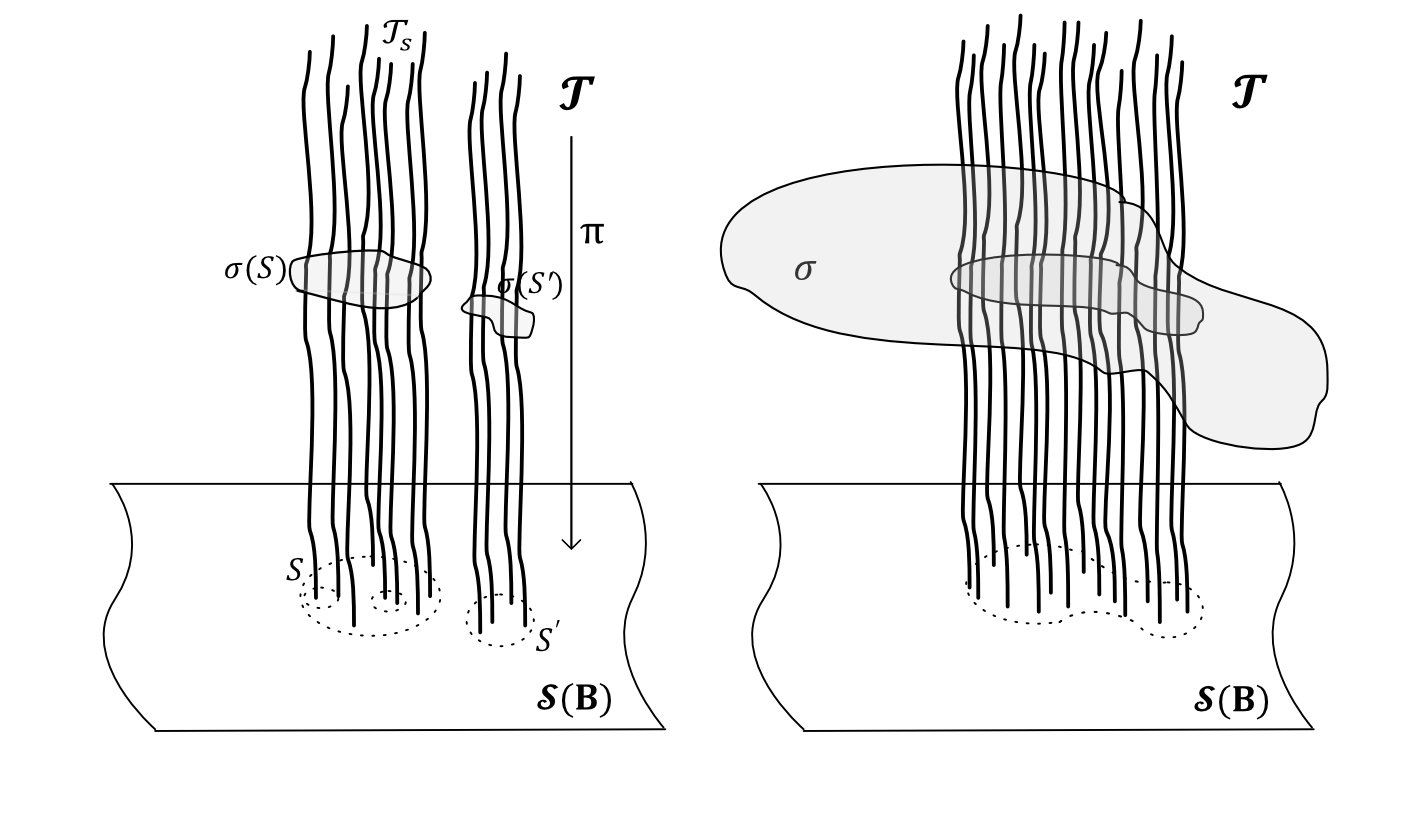
\includegraphics[width=.7\textwidth]{ART_Woszczek/Woszczek.jpg}
\caption{}\label{woszczek-fig1}
\end{figure}

In fact, what is of crucial importance is that, due to the existence of ultrafilters, the very notion of physical state as a~catalogue of the actual properties of $O$~becomes straightforward; each physical system has its own Einsteinian ‘being-thus', and, moreover, there is no difficulty in extending this notion to the whole universe (world-$\Psi$) taken as a~mechanical system of $O$'s. This means that any ontic contextuality of states is absent, and there is only one global ‘context' of coexisting properties without restrictions, which is encapsulated by the metaphysical catchword ‘Absolute (panoptical) Observer'.

Note that since the ultrafilters on $\bm{B}$ simultaneously generate the full Boolean algebra of all the global sections of $\bm{\mathcal{T}}_{\mathcal{S}}$, that is $\bm{B\cong\Gamma}_{\mathcal{S}}(\mathcal{T})$, one gets the algebra of the classically possible (Leibnizian) mechanical worlds, which is already built from the very beginning into the unitary logical framework. The curious ‘mirroring' feature of the latter is that it is \textit{exactly the same logic} which governs the domains of the possible and the actual, hence there seems to be nothing special about possibility \textit{per se} -- in fact, it is difficult to comprehend why the actual would be ontically distinguished as ‘fully existing'. That is why thinkers like Leibniz needed a~ladder of additional metaphysical constraints as rules of the world selection, or foreknowing God's one-moment choice, while in the classical deterministic cosmology there is always the problem of the extremely improbable boundary conditions and the unpleasant cosmological fine-tuning of the initial (or final) world- $\Psi $ as a~bare fact. It looks like the domain of possibility was fully modelled upon the domain of actuality, and the probabilities for the latter could be consistently pre-assigned only after some complete universe of logically possible states of affairs, i.e. the full Boolean algebra $\bm{\Gamma}_{\mathcal{S}}(\mathcal{T})$, is fixed (that is how the probability of ‘improbable boundary conditions' is assessed).

Even if one prefers the indeterministic ontology and objective (noncontextual) dispositions or propensities, like e.g. Karl Popper
%\label{ref:RNDlNn26X3DSB}(1967),
\parencite*[][]{popper_quantum_1967}, %
 it is tacitly assumed that there is no way beyond the Kolmogorovian measure based on $\bm{\Gamma}$. The reason behind this premise is not just PSR and the requirement of concordance between (i) and (ii), it lies much deeper, in ontological \textbf{DOR}: one needs a~complete basis of definite (Boolean) elements for the probabilistic measure, and then (\textit{i}) and (\textit{ii}) can be handled in a~unitary manner. In the end, there is no way out of the Boolean universe here. The logical state structure $\bm{\Gamma}_{\mathcal{S}}(\mathcal{T})$ in physics is thus a~full realization of the paradigmatic ontological intuition, since being means being definite \textit{and} being a~part of some fully determinate, consistent whole, which brings forth, as a~sort of a~byproduct, the idea of panopticality or a~detached observer. One may sum this up by saying that classical ontology favours the actual and the definite, paying the price of making the potentiality a~mirror image or an expanded shadow of the actual.

In the quantum regime, the rules of the game change drastically. A~lattice of propositions about the properties of a~quantum system $O$ (which may also be multipartite) forms an orthomodular $\sigma $-orthoposet $\bm{\mathfrak{L}}(\mathcal{H})$, being isomorphic with the lattice of closed subspaces of the complex Hilbert space $\mathcal{H}$ associated with $O$, which is complete if it is ordered by inclusion (for simplicity we limit ourselves to cases when $\mathcal{H}$ can be constructed at all, but it can be generalized to all types of $W^{\ast}$-algebras of observables, see
%\label{ref:RNDYwzuYMFRzx}(Döring, 2005)
\parencite[][]{doring_kochenspecker_2005}%
). The sheaf-theoretic construction for quantum observables may be achieved in general as follows. Let a~topological space $\mathcal{L}_{\bm{\mathfrak{L}}(\mathcal{H})}$ be a~family of all Boolean (commutative) subalgebras $L$ of $\bm{\mathfrak{L}}(\mathcal{H})$ ordered by inclusion ${\subseteq}$, and let us have a~required Boolean homomorphism (the Kochen–Specker valuation) $h:L\to \bm{2}$ for any $L_i{\in}\mathcal{L}_{\bm{\mathfrak{L}}(\mathcal{H})}$. We can define the partial ordering $\leq$ for pairs $(L_i,h_i)$, given by: $(L_1,h_1){\leq}\left(L_2,h_2\right)$ iff $L_1{\subseteq}L_2$ and $\left.h_1=h_2\right|L_1$, associated with the respective topology of $\mathcal{L}_{\bm{\mathfrak{L}}(\mathcal{H})}$. Every Boolean subalgebra $L_i$ in $\mathcal{L}_{\bm{\mathfrak{L}}(\mathcal{H})}$ belongs to some maximal Boolean subalgebra (a maximal quantum observable), which forms a~(quasi-) classical \textit{context} $\bm{\mathfrak{M}}$.

Now the \textit{quantum spectral sheaf} (over the base space of quantum observables or spectral algebras), the closest analogue of the classical $\bm{\mathcal{T}}_{\mathcal{S}}$ we get, is a~triple $\bm{\Phi}_\mathcal{L} = (\Phi, \pi, \mathcal{L}_{\bm{\mathfrak{L}}(\mathcal{H})})$, with $\Phi_{L_i}=(L_i,h_i:L_i{\in}\mathcal{L}_{\bm{\mathfrak{L}}(\mathcal{H})})$ and a~projection as a~surjective local homeomorphism (étale map) $\pi :\Phi \to \text{[27F6?]}$ from the sheaf space $\Phi $. A~continuous local section (of the projection $\pi$) over some subset $M \in \mathcal{L}_{\bm{\mathfrak{L}}(\mathcal{H})}$ is a~map $\sigma: M \to \Psi$, $\pi \circ \sigma =\mathit{id}_M$, and the images of local sections naturally induce the topology for the whole étalé space $\Phi$. That is so because for every $L_i \subset M$ we obviously get $\{0,1\}$-values of the sheaf, $\sigma (L_i)=(L_i,h_i)$, with the proper restriction condition: $\sigma (L_1)=(\left.L_2,h\right|L_1)$ for every $L_1\subseteq L_2$, which always guarantees the local compatibility of sections as a~crucial fact about the quantum observable values. Due to Gleason's no-disturbance principle for $\mathcal{L}_{\bm{\mathfrak{L}}(\mathcal{H})}$, the probability for obtaining some value cannot depend on a~valuation of some other compatible observable, which gives the properly behaving, i.e. additivity satisfying, probabilities for $\bm{\mathfrak{M}}$'s
%\label{ref:RNDyf3gAnFNxU}(Gleason, 1957).
\parencite[][]{gleason_measures_1957}.%
\footnote{In the operational framework, one might call this central property the ‘noncontextuality of projective measurements'. However, it should be remembered that it is a~purely algebraic feature of the whole quantum structure, and not just the statistical characteristics of particular sets of measurement outcomes.} Hence the latter define subclassical ‘patches' within the full quantum $\bm{\mathfrak{L}}(\mathcal{H})$, and the essence of the generic quantum complementarity is that it is not possible to have the full $\{0,1\}$-valuations (i.e. the Kochen–Specker states) over two different $\bm{\mathfrak{M}}$'s at the same time.\footnote{See e.g. 
%\label{ref:RNDZs9dzkK0Uy}(Heunen, Landsman and Spitters, 2012)
\parencite[][]{heunen_bohrification_2012} %
 for a~purely operator-algebraic account of quantum complementarity, and 
%\label{ref:RNDUOLqvF5lBt}(Heunen, 2012)
\parencite[][]{heunen_bohrification_2012} %
 for a~general categorical approach in terms of dagger monoidal kernel categories.}

The (Bell–)Kochen–Specker Theorem in the sheaf-theoretic formulation simply says that if a~Hilbert space $\mathcal{H}$, representing the physics of a~system $O$, is of $\mathit{dim} > 2$, then the spectral sheaf $\bm{\Phi}_{\mathcal{L}}$ on $\mathcal{L}_{\bm{\mathfrak{L}}(\mathcal{H})}$ has \textit{no global sections}. Thus, we have a~strong topological obstruction, which makes the unrestricted extending of local $\sigma$ impossible if the global consistency of valuations $\sigma (L)$, as in the case of $\sigma (S)$ for $\mathcal{T}_{\mathcal{S}}$, has to be preserved (ultimately, that is what the objectivity of states (i) and the EPR intuition about the definite ‘elements of reality' do unconditionally demand). A~global Boolean ‘context' for mechanics does not exist, and only single local contexts $\bm{\mathfrak{M}}$, as defined by quantum spectral algebras, can be regarded as being definite, hence the whole idea of synchronic $\{0,1\}$-properties, objectively preexisiting and pertaining to $O$ as ‘states', gets into fatal trouble.

In consequence, what is actual, i.e. a~definite fact F~from (i), is only a~\textit{random local section} $\sigma (L)$ of $\pi$ in a~particular definite $\bm{\mathfrak{M}}$, and that physically relativizes the valuation $h$ itself, which is a~contingent relation of $O$ to some exosystem $O'$ that induces the particular $\bm{\mathfrak{M}}$.\footnote{Due to the standard minimal interpretation of the situation, quantum mechanics cannot be -- and is not -- metaphysically realist in the \textit{classical} meaning of the term, which is quite obvious. But the stronger claim that it cannot be realist at all (in any acceptable sense) is premature and overly dependent on the classical metaphysical framework of actuality and its ‘mirroring' possibility, that is $\bm{B\cong\Gamma}_{\mathcal{S}}(\mathcal{T})$. In fact, it rests on the acceptance of \textbf{D} as a~putative necessary condition of realism \textit{per se}.} Quantum mechanics simply lacks the constructive backbone of its classical predecessor. Before I~discuss what this means for any ontological account of potentiality, it is important to indicate why this topological obstruction has nothing to do with the classical epistemic contextuality and should be physically dealt with as a~fully ontic property. These arguments are thus based on strictly physical, including experimental, considerations, being at least relatively independent from contestable metaphysical presuppositions, and they range from quantum-informational to thermodynamical aspects. In essence, $\bm{\Phi}_L$ induces the totally nonclassical structure of \textit{physical} probability and entropy, and that only in turn effectively restrains ontologies with definite states or dispositions modelled after $\bm{\Gamma}_{\mathcal{S}}(\mathcal{T})$ (I shall go back to the latter point in the next section).

Firstly, the topological obstruction on $\bm{\Phi}_L$ gives rise to the entirely novel physics of information processing in Nature, the objective (non-epistemic) quantum regime, which has nothing to do with human labs and disturbance-producing experiments. At the level of the latter, due to the contextuality or algebraic ‘locality' of $\sigma (L)$, it is impossible to perfectly distinguish some unknown pure nonorthogonal quantum states, and thus to determine in one shot an unknown state on a~single copy, however weak the conceivable measurement is
%\label{ref:RNDuquyajTMxC}(D'Ariano and Yuen, 1996).
\parencite[][]{dariano_impossibility_1996}. %
 One can do that only randomly with the Holevo–Helstrom probability $p_{\mathit{HH}} \leq \frac{1}{2}(1+\sin \theta )$ of successful guessing, for the equal probability of the preparation of each state and $\theta $ being an angle between two vectors in $\mathcal{H}$. However, any purely epistemological explanation of this bound on \textit{discriminability}\footnote{If multiple copies of transmitted states are physically available, the empirical probability of successful guessing significantly increases with the number of copies and the specific measurement strategies involved. Note that the probability $p_{\mathit{HH}}$ is also an entropic measure, the so-called min-entropy 
%\label{ref:RNDd1WkncgrLj}(Konig, Renner and Schaffner, 2009).
\parencite[][]{konig_operational_2009}.%
 } is misleading. First note that the related basic quantity $\cos ^2\theta $ is a~probability that the two corresponding states may be confused, that is, if one of them is ‘measured', or, better still, filtered in the basis (or context) of the other, it passes the test, and vice versa. Now, it can be quantitatively estimated for such a~quantum nonzero \textit{confusability} of states how much any (quasi-)classical simulation which is maximally epistemic (i.e. assumes the quantum measure to be just a~measure of classical ignorance about a~distribution of the underlying actual ontic (hidden) $\{0,1\}$-states) must fail for $\mathit{dim} \mathcal{H} > 2$, while the failure grows dramatically with $\mathit{dim}\rightarrow {\infty}$ 
%\label{ref:RNDtAuOEE49Hs}(Leifer, 2014; Barrett et al., 2014; Branciard, 2014),
\parencites[][]{leifer_ensuremathpsi-epistemic_2014}[][]{barrett_no_2014}[][]{branciard_how_2014}, %
 which has already been tested with success 
%\label{ref:RND9AEBTyy5fL}(e.g. Ringbauer et al., 2015; Liao et al., 2016).
\parencites[e.g.][]{ringbauer_measurements_2015}[][]{liao_experimental_2016}.%
\footnote{Recently, Schmid and Spekkens 
%\label{ref:RNDU3j8HTLsy0}(2018)
\parencite*[][]{schmid_contextual_2018} %
 have shown that any noncontextual ontological model must satisfy some nontrivial trade-off relation between the Holevo–Helstrom bound and confusability, which is violated by quantum systems as a~clear indicator of ontic contextuality. More precisely, for a~given confusability the optimal quantum trade-off allows more success rates than the classical noncontextual one. This no-go result is particularly important since it is theory-independent and can provide a~clean operational account of (non)classicality. } This means that BKS is sufficient to rule out any maximally epistemic models (including noncontextual preparation models) which try to treat the quantum measure like the quasi-classical measure, which it is not. Apparently, there is no hidden reality with facts satisfying \textbf{DOR} -- no ‘elements of reality' to be mechanically disturbed by our clunky experiments in spacetime, and this seems to be a~source of quantum computational gain.

But there is, secondly, much more to contextuality and indistinguishability (which in turn have some surprising relation to the causal stability of spacetime). The latter makes it impossible to build perfect quantum cloning or deleting machines due to the quantum no-cloning, no-broadcasting and no-deleting principles. If it were possible to perfectly discriminate unknown nonorthogonal states beyond the Holevo–Helstrom bound, one could freely produce their copies and thus easily violate the no-cloning prohibition (in fact, state discrimination may be regarded as a~form of cloning). Although there indeed exist noncontextual ontological models which are able to recover some substantial aspects of the no-cloning phenomenology, what is a~purely quantum advantage induced by ontic contextuality is a~strictly higher maximum fidelity of cloning as related to the confusability of states
%\label{ref:RND33nGhk6wyN}(Lostaglio and Senno, 2020).
\parencite[][]{lostaglio_contextual_2020}. %
 It is again contextuality as a~topological property which precludes any fully classical simulation of no-cloning and, presumably, no-deleting.

Now, the physical fact is also that if it was possible e.g. to delete an unknown quantum state available in two copies or exactly clone an unknown state, one could send faster-than-light signals in the Universe and infringe its causal order
%\label{ref:RNDNg1An1jeDy}(Gisin, 1998; Pati and Braunstein, 2003).
\parencites[][]{gisin_quantum_1998}[][]{pati_quantum_2003}. %
 One can still perform a~quantum approximate or just probabilistic cloning, but even in such cases opening a~nonlocal signaling channel is ruled out 
%\label{ref:RND5XTekE1MJm}(Pati, 2000; Bruss et al., 2000).
\parencites[][]{pati_probabilistic_2000}[][]{bruss_approximate_2000}. %
 It is well known that there is a~much larger space of strong nonsignaling (more nonlocal) correlations, which also do not allow free cloning, but are not achievable on quantum systems 
%\label{ref:RND5Hv1lQBXdc}(Masanes, Acin and Gisin, 2006),
\parencite[][]{masanes_general_2006}, %
 however general contextuality itself provides a~specific insight even here. Every Kochen–Specker proof can be used to derive the Bell (bipartite) inequalities \textit{maximally} violated by quantum theory and with their values being at the same time \textit{exactly on the boundary} of infringing the Lorentz invariance, but never actually doing so 
%\label{ref:RNDkkf9opqtLz}(Aolita et al., 2012).
\parencite[][]{aolita_fully_2012}. %
 These special maximal contextuality-based correlations are particularly interesting, since the corresponding probability distributions for actual events have a~null set of local models able to simulate them, but nevertheless, in this extremal case, they precisely accord with the relativistic causality. Most philosophical discussions concerning the nonclassical probability distributions have usually been focused on the vexing problem of nonlocality between actual, definite systems in spacetime, but the correlations of this sort reveal that the source of quantum advantage in general resides rather in the \textit{full absence of actual} (spatiotemporal) $\{0,1\}$-properties, that is, in objective indefiniteness from the Kochen–Specker-type sets. One may surmise that such a~sector of tangent concordance between contextuality as a~topological constraint (without any reference to the speed of light or the physics of interaction) and the nonsignaling bound (causal structure of classical spacetime)\footnote{Of course, constraints induced solely by the Kochen–Specker contextuality cannot reproduce the full statistical constraints on quantum nonlocality, since the former are more general -- they just do not include the complex product structure typical for entanglement in multipartite systems.} cannot be a~mere coincidence and is more readily an ontic feature of the Universe, without any dependence on the messy operations in labs.

Finally, there is one ultimate judge in physics, and this is thermodynamics. Quantum histories (let's call them q-histories) are thermodynamically different from classical histories, since their entropic characteristics deviate extremely from those of classical histories solely due to ontic contextuality. In particular, q-histories of single indivisible systems violate the simplest 5-cyclic entropic noncontextuality inequality in time
%\label{ref:RNDgSLqUaae3n}(Chaves and Fritz, 2012),
\parencite[][]{chaves_entropic_2012}, %
 as well as the 5-cyclic Kurzyński–Ramanathan–Kaszlikowski inequality for conditional entropies 
%\label{ref:RNDDCHjGRmRvo}(Kurzyński, Ramanathan and Kaszlikowski, 2012),
\parencite[][]{kurzynski_entropic_2012}, %
 which would be impossible if the underlying structure of events were $\bm{\Gamma}_{\mathcal{S}}(\mathcal{T})$. This is of fundamental significance as far as it needs neither the introduction of the aforementioned correlation functions of single outcomes nor averaging over some hypothetical hidden variables, as in the Bell model. Moreover, one can construct a~\textit{purely thermodynamic} formulation of the (Bell–)Kochen–Specker Theorem and show that the quantum entropic contextuality is a~very strong obstruction to any putative ‘thermodynamic realism' based on the presumed Kolmogorovian measure and hidden dispersionless states 
%\label{ref:RNDjejiqghtlM}(Jia et al., 2018).
\parencite[][]{jia_entropic_2018}. %
 If the resulting quantum entropic monogamy relations\footnote{Monogamy relations are an important feature of quantum correlations as quantitative constraints on their sets, which limit the shareability of information between distinct parties 
%\label{ref:RNDxEsxRzprkD}(see e.g. Dhar et al., 2017).
\parencite[see e.g.][]{dhar_monogamy_2017}. %
 They are closely related to the no-signaling principle and its generalized form, Gleason's no-disturbance principle (for sets of compatible measurements). In the thermodynamic framework studied e.g. in 
%\label{ref:RNDhChdWQHp7p}(Jia et al., 2018),
\parencite[][]{jia_entropic_2018}, %
 the straightforward monogamy relations are constructed for entropic Shannon-type inequalities defined on sets of measurements.} were violated for sequential operations in time, it would also be possible to signal into the past and infringe the causal structure of spacetime, which quantum protocols cannot do. Thus, ontic contextuality induces a~more general, consistent thermodynamics, and ontology rather has to come to terms with this nontrivial fact without trying to seek rescue in epistemology.

\section{Quantum potentiality is real indefiniteness, not counterfactual possibility}
A~natural starting point for quantum ontology is the conclusion that the problem is not quantum mechanics itself, in particular BKS, but rather the metaphysical assumption concerning what counts as being and what is non-being, that is, in short, \textbf{DOR}. This is quite interesting since only rarely does physics impose such pressure upon a~basic metaphysical intuition which often seems to be a~pure \textit{a~priori} of physics. Of course, this does not happen without some serious opposition, since there might be doubts about whether the pressure is legitimate or whether physics should be allowed to demand drastic moves at the primitive level of ontology. I~fully agree that no physical restrictions can just pick out a~particular metaphysics as the right one
%\label{ref:RNDvzqWFtHLse}(cf. e.g. Hawley, 2006; French, 2014),
\parencites[cf. e.g.][]{hawley_science_2006}[][]{french_2014}, %
 and neither can they solve metaphysical dilemmas like determinism vs. indeterminism, since the constructive inventiveness of general metaphysics is illimitable, but, nevertheless, the naturalistic ontology of physics is not so unconstrained in its dealing with contextuality.

The indicated opposition to the overtly ontological interpretation of contextuality makes quite clear an uneasy tension between physics and theoretical metaphysics, which is discernible in discussions on both sides. In this specific case, it is not so much a~methodological problem, but rather a~relatively rare clash between genuinely fundamental metaphysical assumptions, spawning a~whole class of shared realistic intuitions (concerning e.g. ‘state'/‘fact', ‘disposition' or ‘possibility'), and the equally fundamental structure of the highly confirmed, although falsifiable, physical theory, and that indeed makes any choice a~delicate issue. On the one hand, it seems rather unsurprising that one tries to avoid abandoning basic intuitions that are a~sort of common ground in metaphysics. For example, it is instructive to observe how \textbf{D} and counterfactuality still play a~guiding constructive role even in novel philosophical conceptualizations of ontic indeterminacy
%\label{ref:RNDoNglIzrWEH}(e.g. Akiba, 2004),
\parencite[e.g.][]{akiba_vagueness_2004}, %
 which illustrates the previously mentioned ‘mirroring feature' of such models. On the other hand, there has been considerable progress in the physics of contextuality, both experimental, e.g. concerning entropic tests in state-independent scenarios 
%\label{ref:RNDysF0Z1eXlL}(Qu et al., 2020),
\parencite[][]{qu_experimental_2020}, %
 and theoretical, related to the theory-independent, purely operational accounts of contextuality (which are beyond the scope of this paper). Both make the pressure on the ontology of physics constantly grow, analogously to the historical case of the theory-independent Bell inequalities. Hence, the clash seems to be more and more conspicuous and hard to ignore.

One of the common answers to contextuality is adopting the view that if $\psi$ is not a~catalogue of definite actual properties, one could just accept indeterminism with physical possibilities as an ingredient of ontology, which might solve the riddle. However, the basic lesson from BKS is that merely to keep \textbf{DOR} unscathed is simply \textit{not} enough, since possibilistic indeterminism is neither sufficient nor necessary to account for contextuality. For example, the most natural choice for a~classical dispositionalist is to assume that an actual system $O$ always possesses a~set of definite intrinsic potential properties, which is a~consistent catalogue of its possibilities represented by $\psi$ and the full set of probabilities calculated from the complex amplitudes. According to such a~view, the actual outcome of interaction with $O$ would be just the indeterministic manifestation of one such pre-existing possibility pertaining to the system.

But BKS itself, as a~strong topological obstruction on $\Phi_{L_i}$, makes such a~model untenable, that is, taking $\psi $ to be a~set of objective, pre-assigned possibilities that reside in $O$ results in physical contradiction. The first simple proofs of this theorem have been offered by Adán Cabello
%\label{ref:RND3mfitaHi2a}(Cabello, 1999a)
\parencite[][]{cabello_quantum_1999-1} %
 who used the GHZ-like construction (without inequalities and probabilities) for three pairs of systems, as well as the Hardy-like proof for two pairs of systems. In fact, every quantum Bell-like scenario with entangled systems is just a~particular realization of the contextuality scenario for compound systems, hence it is a~\textit{statistical} illustration of the breakdown of the notion of local intrinsic possibilities pre-assigned to subsystems. One may easily demonstrate that it is in each case related to the noncontextual assignments of properties, even if they are only probabilistic correlations and nothing more 
%\label{ref:RNDuIqWvj5vIS}(Cabello, 1999b).
\parencite[][]{cabello_quantum_1999}. %
 The maximally nonlocal correlations discussed in the previous section are just an explicit example of this.

Furthermore, one may use the general information-thermodynamic Bell–Kochen–Specker obstruction and the resulting quantum monogamy relations from simple Shannon-like inequalities
%\label{ref:RNDxCE6edyPNT}(Jia et al., 2018)
\parencite[][]{jia_entropic_2018} %
 as a~direct proof of the impossibility of constructing a~model with the physical sources of stochastic behavior intrinsic to systems, whether they are simple or composite. Quantum entropies themselves, not just some particular sets of purely statistical correlations in space and time, rule out pre-assigned internal dispositions that might stochastically manifest in direct response to some external stimuli. This is, as I~indicated, because the Kolmogorovian probabilistic measure completely breaks down for $\bm{\mathfrak{L}}(\mathcal{H})$, the quantum probabilities are not convex combinations of $\{0,1\}$-states, and this has nothing to do with some local mechanical disturbance of state or the epistemic conditions of access to the properties of some $O$. The trouble lies in the classical understanding of a~(pre-assigned, Boolean) property, whether categorical \textit{or} dispositional, that is, in Einstein's ‘being-thus', which is why his principle of separability cannot work. For example, statistical Liouville mechanics with a~strong epistemic restriction (i.e. respecting some specific constraints on observables), equivalent to Gaussian quantum mechanics 
%\label{ref:RNDuzYOzpA4up}(Bartlett, Rudolph and Spekkens, 2012),
\parencite[][]{bartlett_reconstruction_2012}, %
 is unable to recover quantum contextuality, either state-dependent or state-independent, including the full range of nonlocal correlations for Bell-like scenarios.

Now it is possible to identify the deep metaphysical source of permanent confusion about quantum contextuality as the tacit adoption of \textbf{DOR} and its philosophical consequences, such as e.g. the working metaphysics of the Boolean ‘elements of reality' (states) collectively fused into some postulated actual world-$\Psi$, the credence in the definite counterfactual observables (Leibnizian possibilities), as well as the Principle of Sufficient Reason, which encourages mechanical reasoning about producing the outcomes. On the mathematical level, their failure is effected by the total breakdown of the structure $\bm{\mathcal{T}}_{\mathcal{S}}$ and the corresponding commutative probability theory, but a~decision to reject \textbf{DOR} has far-reaching consequences, not just for standard philosophical counterfactual analyses, which are of no use here, but for understanding the underlying physics. The problem begins with the very vocabulary of quantum mechanics inherited from the classical theory.

The term ‘contextuality', as used in the Bell-like sense, has been employed in the framework of the hidden variable models, that is $\bm{\mathcal{T}}_{\mathcal{S}}$, and it may still give the impression that it is the mechanical ‘context of measurement', or the internal state of the apparatus, which somehow ‘influences'\footnote{It has been the Bohrian or, more generally, Copenhagen tradition which introduced such the problematic terminology of ‘influence', though, to be fair, one must admit that it was construed by Bohr purely epistemically as an ‘influence on the conditions of possible experience'. The very idea of ‘context' also has a~strongly epistemic flavor. Such a~quasi-Kantian formulation is unworkable from the point of view of ontology. } the outcome by covertly selecting some subset from among the inferred, physically pre-existing possibilities, even nonlocally in spacetime
%\label{ref:RNDNfBJJHCb0R}(for a~methodic critique see e.g. de Ronde, 2017).
\parencite[for a~methodic critique see e.g. de][]{de_ronde_unscrambling_2017}. %
 However, the breakdown of $\bm{\mathcal{T}}_{\mathcal{S}}$, i.e. the absence of ultrafilters on the presumed world-$\Psi$, is most naturally equivalent to the \textit{global collapse of the valuation definiteness} in the fully ontological sense, which means that quantum potentiality is not any sort of Leibnizian possibility and has nothing to do with the classical counterfactuality of measurements. Thus, the ontological source of contextuality from the BKS formulation on $\mathcal{L}_{\bm{\mathfrak{L}}(\mathcal{H})}$ is rather the purely physical, real indefiniteness (the indeterminacy of being) \textit{and} the associated purely ontic randomness in the quantum regime. Abbott et al. 
%\label{ref:RNDadugYS9dhf}(2012)
\parencite*[][]{aolita_fully_2012} %
 have proved the stronger version of BKS (without assuming the global Kochen–Specker valuation), in which it is possible to precisely identify the objectively (provably) indefinite values of observables, and hence to produce strongly certified quantum random sequences which are Turing incomputable. In fact, it can be shown that such value indeterminacy is ubiquitous if only one particular observable is locally fixed to be value definite 
%\label{ref:RND4e3HJ4ghV3}(Abbott, Calude and Svozil, 2014).
\parencite[][]{abbott_value-indefinite_2014}.%


In this sense, physical indeterminacy as a~quantum resource seems to be almost everywhere in Nature, while definiteness is a~local phenomenon, which makes indefinite potentiality physically fundamental, and the definite actuality secondary. It is the former that is \textit{the} main engine of quantum mechanics, and makes possible quantum information processing and nonlocal effects without the slightest infringement of the Lorentz invariance, since what is indefinite and does not exist in spacetime cannot be ‘transmitted' or ‘sent' in it (as a~definite spatio-temporal being can be).

Some misconceptions in construing quantum theory may indeed result from imposing \textbf{DOR} as a~tacit ontological premise and explicating quantum potentiality through the category of actuality, i.e. taking the latter to be ontologically primary and pervasive. But what we have in the quantum regime is an exact reversal of the classical mirror-like relation of actuality and possibility, the latter being constructed according to the former within the unified logical universe $\bm{B \cong \Gamma}_{\mathcal{S}}(\mathcal{T})$. As a~topological obstruction, BKS contravenes this relation, making the potentiality ontic, primitive and \textit{dissimilar} to the actuality that cannot simulate or encompass the former within such a~Boolean logical universe. It is precisely this dissimilarity and incomputability which indicates that the post-classical terminology of both the counterfactual ‘possibility' and ‘measurements' of actual states is misleading, for it still assumes the metaphysics of the ‘Absolute (panoptical) Observer'.\footnote{However, the difference between pure quantum \textit{potentiality} and classical \textit{possibility} is not verbal or purely metaphysical, since the issue is not speculation about possible observers but the physical structure of quantum processes as encoded topologically in $\bm{\Phi}_\mathcal{L}$.} In particular, the breakdown of \textbf{DOR} and the Principle of Sufficient Reason would mean that there is no operative rule, law or reason determining the transition from the (generic quantum) potential to the (spatio-temporal) actual, which is ‘irrational' or ‘alogical' in the fully ontological sense %
%\label{ref:RNDk2hyf52eNB}(cf. e.g. Bub, 2014).
\parencite[cf. e.g.][]{bub_quantum_2014}.%
\footnote{As far as I~know, it was Wolfgang Pauli who first adopted the epistemological term \textit{Irrationalität} from the early Bohr, emphatically insisted on the metaphysical meaning of that ‘irrational actuality' against the currents of the history of Western ontology, and called quantum mechanics the ‘theory of becoming' 
%\label{ref:RNDKNVdf2frw7}(see e.g. Pauli, 1994).
\parencite[see e.g.][]{pauli_probability_1994}.%
} In this case, the Spinozian axiom would be false: \textit{possibile est, ut effectus sequatur, si nulla detur determinata causa}, that is, the operative cause of some definite state of affairs may be an indefinite (non-Boolean) potency.

The breakdown of determinacy does not imply that ontological realism \textit{per se} is impossible or that objective reality itself vanishes into thin air. In point of fact, the aforementioned reversal itself makes quantum potentiality and randomness an effectively \textit{autonomous} agent and a~\textit{physically real} reservoir. For example, entropic contextuality may be utilized in quantum network communication, and indefiniteness in general is critical as a~resource for speed-up in universal quantum computation
%\label{ref:RNDvhzcPou5YV}(Howard et al., 2014).
\parencite[][]{howard_contextuality_2014}. %
 Quantum randomness is autonomous or absolute in the sense that it cannot be physically controlled or influenced by any local agent, it may only be exploited or used as a~means for doing physical work, hence it paradoxically resembles the laws of classical mechanics and, from the point of view of any such agent, is maximally independent. In the quantum realm, there is nothing more real than that.

What is more, the only fully noncontextual, objective element of the quantum algorithm, which is explicitly Lorentz-invariant, is the Born rule that fixes the complete probability distribution for each quantum state (algebraically, $\bm{\mathfrak{M}}$). That noncontextuality is, as the no-disturbance principle, at the centre of Gleason's Theorem and plays a~decisive role for defining the objective concept of generic ‘quantum state' as a~unique measure on $\bm{\mathfrak{L}(\mathcal{H})}$, which is a~situation peculiar to quantum theory.\footnote{In classical Liouville mechanics, one can impose the probabilistic measure on a~phase space freely as reflecting the contingent ignorance of an agent modelling a~system.} Barnum et al.
%\label{ref:RNDPQI0x8PcDl}(2000)
\parencite*[][]{bruss_approximate_2000} %
 have perhaps rightly stressed, from the mathematical point of view, that ‘it is hard to imagine a~cleaner derivation of the probability rule than this'. Philosophically, it is a~hallmark of the quantum reversal, for what is physically real and invariant seems to be a~generic potentiality, even if the universal value definiteness is excluded by $\bm{\mathfrak{L}(\mathcal{H})}$, which cannot support any Boolean measure. If some domains of reality do defy determinacy, one may conclude that the intuition that backs \textbf{DOR} is plainly false.

To make it more express and concrete, let us take an example of a~test of the state-independent contextuality on a~single simple system in time as realized e.g. on single qutrits by Xiao et al.
%\label{ref:RNDHXRAvMBtSK}(2018).
\parencite*[][]{cavalcanti_classical_2018}. %
 In such a~scenario it is possible to guarantee the statistical no-signaling condition between the consecutive measurements by assuming that any disturbance of the future is indistinguishable within an experimental error from the influence of the future on the past. In perfect agreement with BKS, such a~system strongly violates the correlational noncontextuality inequality, which is an empirical manifestation of the topological nonclassicality of the quantum sheaf. The first and fundamental lesson is that there are no \textit{actual} $\{0,1\}$-properties of it just waiting there to be disclosed by sequential measurements.

But there is much more if one acknowledges the reality of dispositions. The first, conservative, strategy is to try to model them by somehow enforcing \textbf{D} as binary valuations on the level of sheer counterfactual possibilities pertaining to that system in each moment. But, as we have seen, it is also structurally excluded on the same grounds as actual $\{0, 1\}$-properties. To say that a~single system carries its intrinsic dispositions in time as its own possibilistic ‘state' makes no sense, since the respective evolving probability distributions are unable to violate the noncontextuality inequalities. The ontological notions of both intrinsic ‘state'/‘properties' and intrinsic ‘disposition' seem misguided unless one accepts a~pervading ‘Ptolemaic' hidden fine-tuning in spacetime.\footnote{For the contextuality-testing scenarios with single systems in time see
%\label{ref:RNDNiImENc7aU}(Cavalcanti, 2018).
\parencite[][]{cavalcanti_classical_2018}. %
 } Thus, taking the BKS and experimental results seriously, I~cannot see any significant gain in invoking world-$\Psi$ and counterfactual (Leibnizian) possibilities as useful metaphysical tools.

Better suited for directly ontological interpretation of the new physical sheaf-structure $\bm{\Phi}_{\mathcal{L}}$ is the second, more radical, strategy. It takes quantum potentiality to be objective (\textit{context-invariant} and \textit{quantifiable}) pure indefiniteness, thus, in line with Abbott et al.
%\label{ref:RNDlh6UODZr1y}(2014),
\parencite*[][]{howard_contextuality_2014}, %
 there are no determinate properties of any system \textit{nor} measures on them before actualization, which might serve as building blocks for spatiotemporal reality and causal interactions, and neither are there laws or rules governing such actualizations. Instead of trying to abide by \textbf{D}, it accepts quantum reversal, that is, rejects the primacy of actuality and binary valuations as a~foundation of ontology, hence actual systems in spacetime cannot be its basic entities at all. Here, in stark contrast to classical mechanics, quantum theory is only about potentiality without mechanical states, \textit{not} about any individual properties or events in spacetime and their putative counterfactual variants as logical shadows.

Although it is beyond the scope of the present paper, one may repeat, for the sake of clarity, that since formally nonlocality is a~special case of general contextuality, it is precisely the objective non-spatiotemporal indefiniteness which should be seen as a~physical source of nonlocal phenomena, not some influence in spacetime or non-Lorentzian (superluminal) action. In this sense, ‘nonlocality' might be treated as a~sort of misnomer, which results from taking for granted the priority of the spatiotemporal actuality composed of determinate ‘states of affairs' in supposed interactions.

\section{The quantum world without real potentiality?}
It is interesting to observe the systemic cost of some strategies to remove ontic contextuality and fully recover \textbf{DOR} (or Specker's ‘Absolute Observer') as a~tacit metaphysical principle. Even if subtheories such as Gaussian quantum mechanics are unable to do that effectively, there are other approaches whose intent is to reduce both the strong ontological import of BKS and ontic randomness. For example, in the many world interpretation, with one evolving multiworld-$\Psi$, contextuality loses any significance for there are no unique states of affairs as actualized properties and possibility merges again with actuality, as in classical $\bm{\Gamma}_{\mathcal{S}}(\mathcal{T})$ but with one crucial difference, namely that these worlds must now be fully included on par, as real elements of physics.\footnote{One of the structural consequences of nullifying the contextuality and invoking counterfactuality are also, not unexpectedly, problems with the many-worlds understanding of the meaning of nonlocal correlations.} One may call this an ‘explosivist strategy' which annuls the uniqueness of outcomes as a~premise of BKS.

In Bohmian mechanics, which is, as a~matter of fact, not just interpretation but rather a~new theory, contextuality results from the mechanical ‘context of an experiment', i.e. an uncontrolled interaction between $O$ and the hidden degrees of freedom of an exosystem (apparatus), hence it looks as if it were utterly trivial: ‘the outcome of an experiment depends on the experiment'
%\label{ref:RNDkmWAbFy7bK}(Dürr, Goldstein and Zanghì, 2013, pp.148–153).
\parencite[][pp.148–153]{durr_quantum_2013}. %
 But since the actual measurement outcomes are strongly relational, it is impossible to say that they are detections of the pre-existing properties of $O$. In fact, Bohmian measurements in our postulated state of cosmological quantum equilibrium are simply ‘false', they do not ‘measure' anything 
%\label{ref:RNDSoW8PTWfMO}(Valentini, 2010, pp.486–488),
\parencite[][pp.486–488]{valentini_broglie--bohm_2010}, %
 and properties, if contextual, are in the Bohmian theory simply nonexistent 
%\label{ref:RNDHj2V0bwaLk}(Dürr, Goldstein and Zanghì, 2013, p.153).
\parencite[][p.153]{durr_quantum_2013}. %
 In other words, the universal timeless world-$\Psi$ is taken very seriously, it is the only \textit{real} wave function 
%\label{ref:RNDMNs80XpA3w}(Dürr, Goldstein and Zanghì, 2013, pp.264–272),
\parencite[][pp.264–272]{durr_quantum_2013}, %
 but, contrary to the many world interpretation, eigenvalues are deprived of any ontological significance, they do \textit{not} correspond to any real subquantum properties at all. One may call this a~double-edged ‘superdeterministic-eliminativist strategy' against BKS, which thwarts ontic contextuality but elevates a~strongly epistemic variant of it, making it a~kind of illusion, due to an assumed ‘subquantum heat death' 
%\label{ref:RNDgl86djh1a3}(Valentini, 2010).
\parencite[][]{valentini_broglie--bohm_2010}.%


A~vindication of \textbf{DOR} and erasing the indefiniteness \textit{in a~single-world ontology} thus have some unpleasant consequences, which are paradigmatically manifest in the Bohmian case. One may evaluate it as the prevailing structural dualism of the latter. In particular, one gets: (\textit{i}) the theoretical postulate of the global world definiteness, i.e. global $\{0, 1\}$-valuation on observables, but an excessively huge amount of information forever hidden, together with the necessary causal fine-tuning for observed correlations
%\label{ref:RNDIHsY2OAzJk}(Wood and Spekkens, 2015)
\parencite[][]{wood_lesson_2015} %
 which operates on the cosmological scale; (\textit{ii}) an \textit{ad hoc} or ‘brutal' segregation of observables into contextual (‘false') and non-contextual ones (the hidden real positions of Bohmian ‘particles'), where the phenomenality of the former also requires cosmological fine-tuning 
%\label{ref:RNDNVmsIVq50J}(Cavalcanti, 2018);
\parencite[][]{cavalcanti_classical_2018}; %
 (\textit{iii}) a~forced divorce between the illusory or epistemic local ‘contextuality' and the essential, genuinely ontological form of it---nonlocal action-at-a-distance 
%\label{ref:RNDugc5J2Vo9d}(Dürr, Goldstein and Zanghì, 2013, pp.154–156);
\parencite[][pp.154–156]{durr_quantum_2013}; %
 (\textit{iv}) the hidden ultimate, definite actuality of $\Psi$ (‘nothing is really potential'), timelessness and the deterministic supercausal order of the postulated subquantum regime, but pseudo-classical possibility, pseudo-randomness and the illusory temporal evolution on the accessible phenomenal level 
%\label{ref:RNDZS3sQCC0fd}(Dürr, Goldstein and Zanghì, 2013, pp.268–271);
\parencite[][pp.268–271]{durr_quantum_2013}; %
 and (\textit{v}) absolute space with absolute rest concealed by phenomenal relativistic spacetime.

In fact, the Bohmian theory insists that almost everything \textit{taken to be} real (ontically noncontextual) is perfectly hidden, and what is \textit{empirically} noncontextual, Gleason's no-disturbance and the Born rule (hence no-cloning, no-deleting etc.), is held to be really violated, albeit not empirically
%\label{ref:RNDcNTStm3xMp}(e.g. Valentini, 2010).
\parencite[e.g.][]{valentini_broglie--bohm_2010}. %
 If one only knew the timeless world-$\Psi$ and the total configuration of Bohmian ‘particles', one \textit{would be} an Absolute Observer, but the theory already makes this forbidden for all local agents trapped in the supposed contingent equilibrium. It looks extremely Ptolemaic as a~construction, from the point of view of Gleason's Theorem and BKS, and if the status of quantum potentiality is like reversal of classical ontology, then the Bohmian theory is like a~forced re-reversal in order to recover \textbf{D}, which produces (\textit{i})–(\textit{v}).

The fundamental metaphysical convictions such as (in)determinism or the meaning of ‘being real' cannot be falsified\footnote{Among the founders of quantum theory it was e.g. Schrödinger who stressed that point and agnosticism regarding the (in)determinism, see
%\label{ref:RNDjzFNtDqxF7}(Schrödinger, 1935).
\parencite[][]{schrodinger_science_1935}.%
}, but some particular interpretations of contextuality have nontrivial physical consequences and are also logically connected to other physical assumptions as well as empirical constraints. These metaphysical and physical assumptions work together, clustered in some consistent metaphysical packages 
%\label{ref:RNDTx53jfycaY}(e.g. French, 2014),
\parencite[e.g.][]{borges_quantum_2014}, %
 hence the real problem is: how high is the price for the metaphysical package we may prefer? It appears that if one is inclined to have \textbf{DOR} intact and ontic indefiniteness eliminated, one must pay a~very high price indeed.

Interestingly, that rather specific predicament sheds additional light on the difficult relation between physics and metaphysics. There seem to be substantial historical analogies between the introduction of the quantum sheaf structure $\bm{\Phi}_{\mathcal{L}}$ into microphysics and the equally revolutionary instillment of non-Euclidean geometry in the physics of spacetime. In the latter case, there have been many attempts to recast the theory of relativity in such a~way that the Newtonian ontology of absolute space and time might be recouped, using e.g. the Lorentz–Kelvin ether theory and the ether interpretations of Einstein's equations. It turned out that such metaphysical motivation brings forth not just the recasting of relativity as some interpretation but also different physical theories, which are unable to compete with general relativity.\footnote{For example, they do not possess singularities (due to the trivial topology) or homogenous curved universes, and introduce \textit{ad hoc} some \textit{completely unobservable} scalar fields.} The introduction of the nonclassical $\bm{\Phi}_{\mathcal{L}}$ under the guise of $\bm{\mathfrak{L}}(\mathcal{H})$ has also provoked some attempts to recast it so as to regain a~sort of pre-quantum ontology based on \textbf{D}. Both quantum theory and relativity are, of course, falsifiable, but the recurring point is that the metaphysical packages associated with them should be dealt with seriously, proportionally to the experimental support, since they are not just a~marginal speculative excess baggage. We suggest that to the extent that metaphysics is interested in the goings-on in the physical world, it is, from the very outset, the ‘twisted' sheaf structure $\bm{\Phi}_{\mathcal{L}}$ itself that should be treated in all seriousness as a~principal guide. In this case, it also seems that it is pure metaphysics itself which may profit from the pressure imparted by physics (even if falsified at some point in the future), since the latter invites to construct new accounts of potentiality which are not one-way dependent on the notion of determinacy.

\section{Conclusion}
Quantum contextuality is a~tough problem for any metaphysical realist, since it puts very restrictive constraints on standard realist strategies which are usually molded after their classical counterparts, for example by sticking to the classical notions of actual state and possibility, like possible spatio-temporal configuration or the intrinsic disposition of a~system. As I~have stressed, the free inventiveness of metaphysics is illimitable, however the interesting case of BKS is that the constructive costs -- both metaphysical and physical -- of adopting these different strategies vary rather markedly, which makes a~choice between them not entirely equivalent or just a~matter of personal taste. In particular, the more one pushes toward retrieving \textbf{DOR} and turning quantum probability into epistemic uncertainty, the more complex and hidden (‘Ptolemaic') the empirically inaccessible sector of a~model becomes, whether explosivist or superdeterministic with fine-tuning and the violation of relativity.

If quantum potentiality is the real indefiniteness \textit{in mundo}, not \textit{in mente}, and \textbf{DOR} collapses as a~basic intuition, then quantum probability itself is a~completely novel type of ontic probability, the probability \textit{sui generis} of physically indefinite properties\footnote{That was already recognized by e.g. von Neumann in the 1930s
%\label{ref:RND6qiqwDYLb4}(Taub, 1962, pp.196–197)
\parencite[][pp.196–197]{taub_quantum_1962} %
 or Pauli 
%\label{ref:RNDayxUqwk5Wh}(1994)
\parencite*[][]{pauli_probability_1994} %
 without relying on any metaphysical analysis. Von Neumann was the first who studied deep connection between quantum structure $\mathcal{L}_{\bm{\mathfrak{L}}(\mathcal{H})}$ and generic quantum probability in the framework of what he called ‘probability logics'.} , which has nothing to do with classical ignorance, determinate counterfactuals, frequencies, or decision making 
%\label{ref:RNDE0zFeHkv0F}(Barnum et al., 2000).
\parencite[][]{barnum_quantum_2000}. %
 This is a~challenge for naturalistic metaphysics, since even philosophical theories of dispositions are constructed with the tacit assumption of \textbf{D}, where complete sets of dispositional properties are clumped in objects or regions of spacetime as some definite ‘elements of reality' producing causal responses. If one takes quantum potentiality to be real, \textbf{OR} might still be perfectly true as a~necessary condition of realism \textit{per se}, there \textit{is} indeed a~fully objective reality, but \textbf{D} is in general false, and Specker's ‘Absolute Observer' is an utter fiction, together with the corresponding counterfactual logic of possibility.

As far as pure ontology is concerned, this is intriguing, since the classical framework for possibility also takes the latter to be completely powerless as a~faint Leibnizian shadow of actuality. If the relation is reversed, it is the indefinite \textit{potentia} that has full objectivity and the power for free actualization, while the definite \textit{actual} is derivative and powerless, like a~much poorer shadow. It is impossible to derive the former from the latter, as it is impossible to acquire the quantum probabilistic measure and quantum correlations in space and time from the (Boolean-)Kolmogorovian measure and shared classical pseudo-randomness
%\label{ref:RNDD8jzeCxefC}(Bub, 2014).
\parencite[][]{bub_quantum_2014}. %
 Thus, the question is: in metaphysics could we accept that autonomous cause or causal power as an agential entity would be entirely non-spatiotemporal and indeterminate? Here I~propose that indefiniteness \textit{in mundo} should be indeed taken as both objective potentiality-power and the generic resource for quantum advantage.

\end{artengenv}


\renewcommand{\theequation}{\arabic{section}.\arabic{equation}}
\begin{artengenv}{Shahn Majid}
	{Quantum geometry, logic and probability}
	{Quantum geometry, logic and probability}
	{Quantum geometry, logic and probability}
	{School of Mathematics, Queen Mary University of London}
	{Quantum geometry on a discrete set means a directed graph with a weight associated to each arrow defining the quantum metric. However, these `lattice spacing' weights do not have to be independent of the direction of the arrow. We use this greater freedom to give a quantum geometric interpretation of discrete Markov processes with transition probabilities as arrow weights, namely taking the diffusion form $\del_+ f=(-\Delta_\theta+ q-p)f$ for the graph Laplacian $\Delta_\theta$, potential functions $q,p$ built from the probabilities, and finite difference $\del_+$ in the time direction. Motivated by this new point of view, we introduce a `discrete Schr\"odinger process' as $\del_+\psi=\imath(-\Delta+V)\psi$ for the Laplacian associated to a bimodule connection such that the discrete evolution is unitary. We solve this explicitly for the 2-state graph, finding a 1-parameter family of such connections and an induced `generalised Markov process' for $f=|\psi|^2$ in which there is an additional source current built from $\psi$. We also mention our recent work on the quantum geometry of logic in `digital' form over the field $\F_2=\{0,1\}$, including de Morgan duality and its possible generalisations. }
	{logic, noncommutative geometry, digital geometry, quantum gravity, duality, power set, Heyting algebra.}




\section{Introduction}

\lettrine[loversize=0.13,lines=2,lraise=-0.03,nindent=0em,findent=0.2pt]%
{T}{}hese are notes growing out of a conference in Kraków with the wonderful question ``Is logic physics?''. My view is yes, obviously. Indeed, I have long proposed \parencite{Ma:pri} to think of Boolean algebras as the `simplest theory of physics', in which case we should be able to see how physical and geometric issues in more advanced theories emerge from structures already present there. If so, then we can see the origin of physics in the very nature of language and the structure of mathematical and physical discourse, a philosophy that I have espoused as {\em relative realism} \parencite{Ma:ess,Ma:pri,Ma:qg3,Ma:sel}. 

One of the things particularly to be explored in this way is the evident role of entropy in the Einstein equations and its deep link with gravity as an ingredient of quantum gravity. My proposal is that while we may not be able to address this in quantum gravity itself, we can try to move quantum gravity ideas back to simplified settings such as finite graphs \parencite{Ma:squ} and Boolean algebras or digital geometry \parencite{MaPac2,Ma:boo} and see if it can be addressed there. The present paper is a step in this direction towards entropy and gravity: we see how probability and irreversible processes can be seen naturally as emerging from quantum geometry. 

Our main new results are in Section~\ref{secmarkov} in the context of graphs, working over $\mathbb{C}$ and $\R$. The idea is to explore a curious feature of quantum geometry applied in the discrete case, namely that the lattice `square length' $x\to y$ need not be same as for $y\to x$. In usual lattice geometry we would be focussed on the edge-symmetric case where these coincide. I will argue that the asymmetric generalisation is the natural setting for probability and non-reversible processes. Thus we consider a Markov process 
\[ f^{new}(x)=\sum_{x\to y} p_{x\to y} f(y)+ (1-p(x))f(x),\]
where $p_{x\to y}$ denote the conditional transition probability from $x$ to $y$ and $p(x)=\sum_{y: x\to y} p_{x\to y}$ for each $x$. If we let $\del_+$ be the finite difference on $\Z$ as the `discrete time' then the Markov process appears as 
\[ \del_+ f= -\Delta f + (q-p)f, \]
where $q(y)=\sum_{x:x\to y}p_{x\to y}$ and $\Delta$ is the canonical graph Laplacian associated to a (typically degenerate) metric inner product defined by the $p_{x\to y}$, in which context it is natural that the value for $x\to y$ need not be the same as for $y\to x$. In fact, the quantities that we should really think of more geometrically as `length' are the negative logs $\lambda_{x\to y}$ of the probabilities, then the shortest length path in that sense is indeed the path of maximum probability. Moreover, the shortest length between two points then makes the space into a Lawvere metric space \parencite{ApCat}. Our point of view is that this is not so much a `generalisation' as what naturally arises in quantum geometry for a discrete space; the real question is why distances are not direction dependent in the continuum limit. Indeed, it could be argued that many processes are
irreversible so already time between events {\em is} measured in a directed way. In the present context, this is reflected slightly differently in our probabilistic interpretation of `distance' as conditional transition probabilities. 

Finally, our point of view leads us to introduce a `discrete Schr\"odinger's process'
\[ \del_+\psi=\imath(-\Delta+V)\psi\]
and to ask what connections $\nabla$ are `unitary' in the sense that $f=|\psi|^2$ remains a probability density when we use the associated Laplacian. We find (see Proposition~\ref{propsch}) that the discreteness results in the evolution of $f$ being a generalised Markov process coupled to a probability current source. Indeed, the discrete Schr\"odinger process being unitary is reversible, so the irreversibility of the Markov process on $f$ is compensated by this source. We construct such a unitary 
Schr\"odinger process explicitly for a 2-state graph $\bullet\leftarrow\!\to\bullet$, finding a 1-parameter family of suitable connections. Unitary matrices are the essence of quantum computing and what we have done is to construct a certain family of them quantum geometrically in the spirit of Schr\"odinger's equation. Another motivation is the recent formulation of `quantum geodesics' \parencite{Beg:geo,BegMa:geo} which indeed includes the actual Schr\"odinger's equation of ordinary quantum mechanics. This work is not immediately applicable due to our use current of discrete time, but these ideas should tie up in future work.

We will use and make reference to a modern constructive `quantum geometry' formalism briefly outlined in Section~\ref{secqg}; see \parencite{BegMa} for details and the extensive literature cited therein. This approach starts with a unital algebra $A$ and choice of differential structure $(\Omega^1,\extd)$ on it and then proceeds to metrics, connections, curvature and so forth. Growing out of many years experience with quantum groups but in no way limited to them, it is very different in flavour from the well-known approach of A. Connes \parencite{Con} coming out of cyclic cohomology and `spectral triples' as abstract `Dirac operators', though with the possibility of useful interaction between the approaches \parencite{BegMa:spe}. 

\begin{figure}\[ 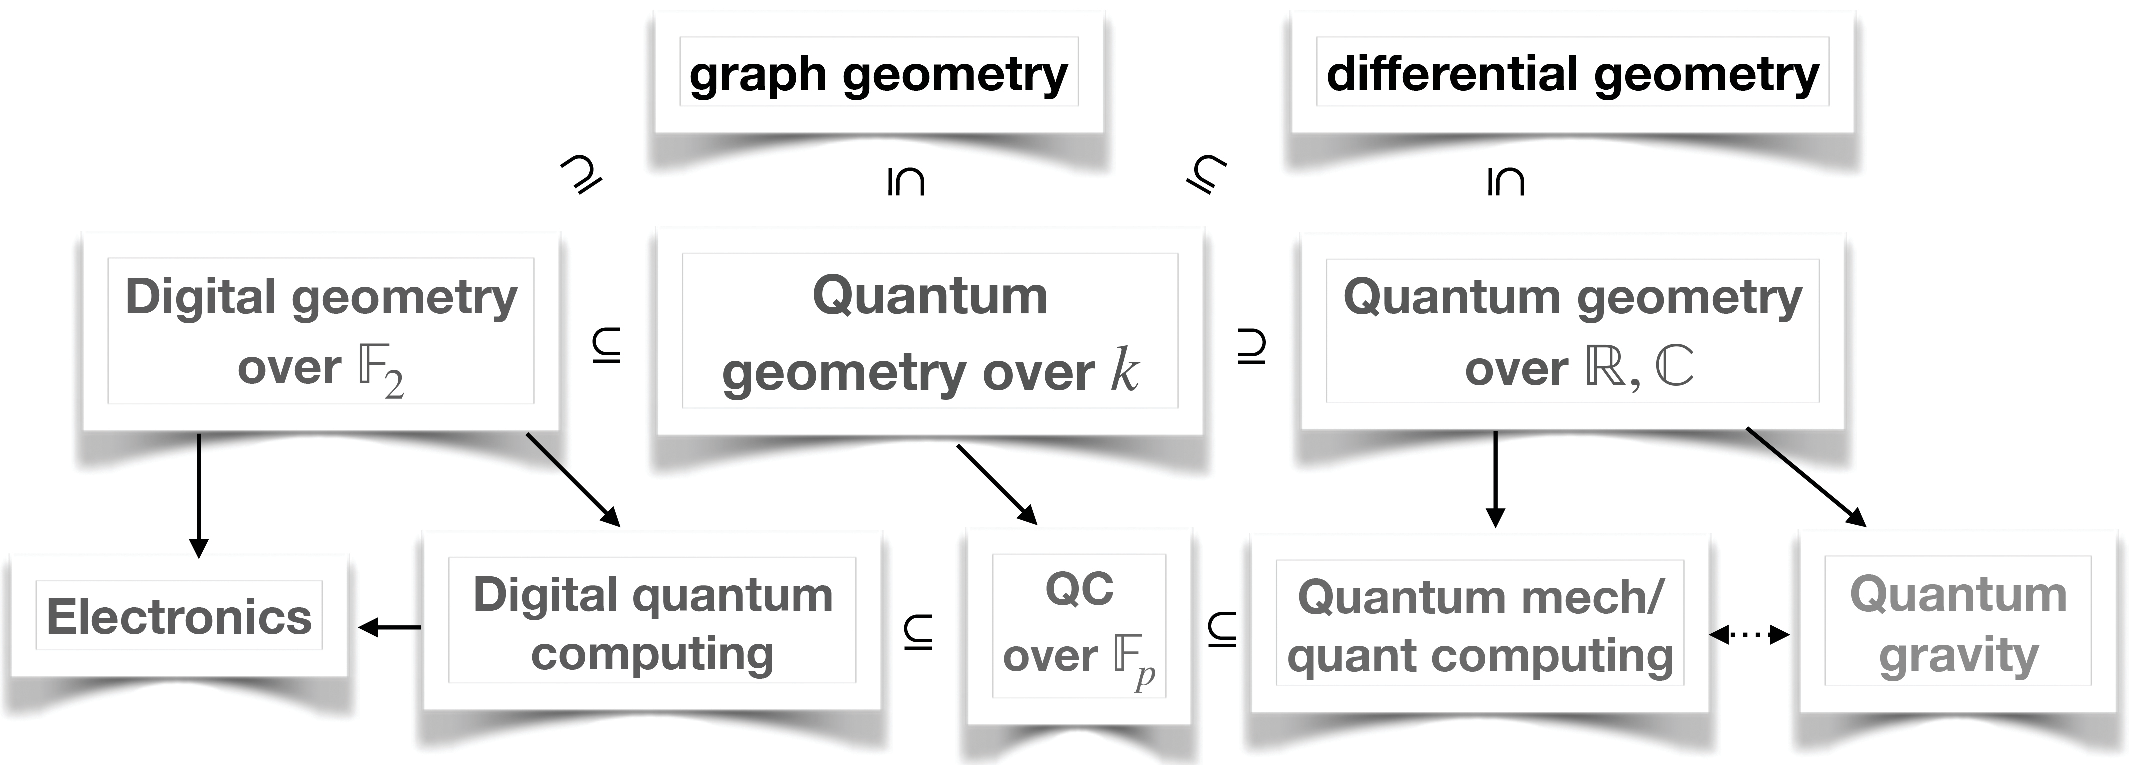
\includegraphics[width=1\textwidth]{ART_Majid/overview-bw.pdf}\] \caption{Quantum gravity and quantum mechanics/computing mediated by quantum geometry over $\mathbb{C}$. Digital geometry as a limiting case.\label{figover}}
\end{figure}

Another aspect of the constructive approach is that it works over any field, which makes possible the `digital' case by working over the field $\F_2=\{0,1\}$ of two elements \parencite{BasMa, MaPac1,MaPac2} and allows in principle the transfer of geometric ideas to digital electronics, see Figure~\ref{figover}. A brief overview is in Section~\ref{secM2} with some modest new results for the quantum geometry of $A=M_2(\F_2)$. In the same vein, one could in theory put something like a digital wave operator for a black hole background onto a silicon chip. A motivation here is again from quantum computing. While in quantum computing, a gate is replaced by a unitary operator (which in turn we envisage could be constructed quantum geometrically, e.g. by a Schr\"odinger process), the essential feature here is the use of vector spaces (the superposition principle) to massively parallelise computations. However, linear algebra works over any field. Hence if we build our gates quantum geometrically then we could specialise them over other fields, including over $\F_2$ as `digital quantum computing'. Even if this did not have the speed benefits of actual quantum computing, it would provide conventionally realisable training wheels for the real thing. 


\section{Outline of quantum geometry} \label{secqg} 

It is well-known that classical geometry can be formulated equivalently in terms of a suitable algebra of functions on the space. The idea in noncommutative or `quantum' geometry is to allow this to be any algebra $A$ with identity as our starting point (and now no actual space need exist). We replace the notion of differential structure on a space by specifying a bimodule $\Omega^1$ of differential forms over $A$. A bimodule means we can multiply a `1-form' $\omega\in\Omega^1$ by `functions' $a,b\in A$ either from the left or the right and the two should associate according to 
\begin{equation}\label{bimod} (a\omega)b=a(\omega b).\end{equation}
We also need $\extd:A\to \Omega^1$ an `exterior derivative' obeying reasonable axioms, the most important of which is the Leibniz rule 
\begin{equation}\label{leib} \extd(ab)=(\extd a)b+ a(\extd b)\end{equation}
for all $a,b\in A$. We usually require $\Omega^1$ to extend to forms of higher degree to give a graded algebra $\Omega=\oplus\Omega^i$ (where associativity extends the bimodule identity (\ref{bimod}) to higher degree). We also require $\extd$ to extend to $\extd:\Omega^i\to \Omega^{i+1}$ obeying a graded-Leibniz rule with respect to the graded product $\wedge$ and $\extd^2=0$. This `differential structure' is the first choice we have to make in model building once we fixed the algebra $A$. We require that $\Omega$ is generated by $A,\extd A$ as it would be classically. 
Next, on an algebra with differential, we define a metric as an element $g\in \Omega^1\tens_A\Omega^1$ which is invertible in the sense of a map $(\ ,\ ):\Omega^1\tens_A\Omega^1\to A$ that commutes with the product by $A$ from the left or right and inverts $g$ in the sense
\begin{equation}\label{metricinv}((\omega,\ )\tens_A\id)g=\omega=(\id\tens_A(\ ,\omega))g\end{equation}
 for all 1-forms $\omega$. This is shown in Figure~\ref{figaxioms}. In the general theory, one can require quantum symmetry in the form $\wedge(g)=0$, where we consider the wedge product on 1-forms as a map $\wedge:\Omega^1\tens_A\Omega^1\to A$ and apply this to $g$. However, we don't need to and moreover we can also work with $g$ non-invertible or $(\ ,\ )$ degenerate. 
 
 \begin{figure}\[ 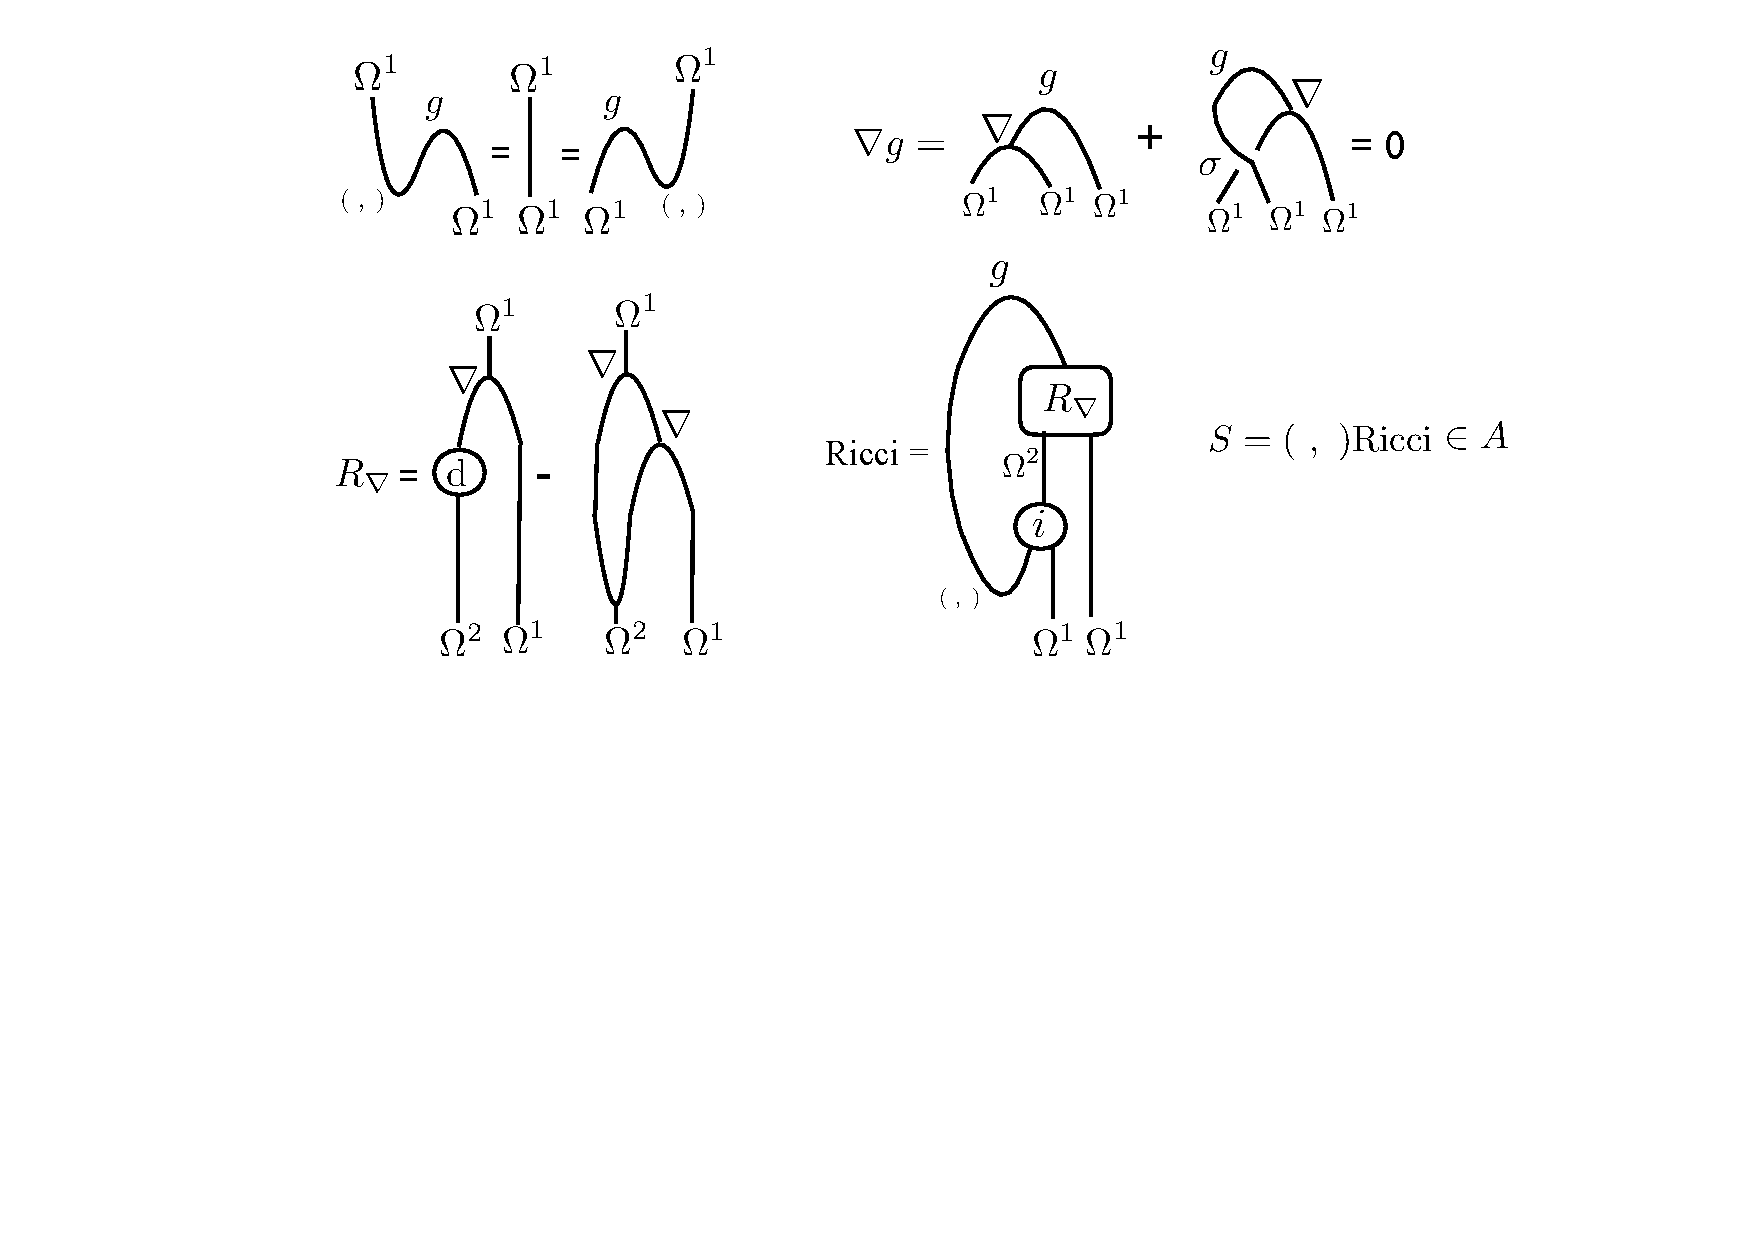
\includegraphics[width=1\textwidth]{ART_Majid/qgaxioms.pdf}\] \caption{Some axioms of quantum Riemannian geometry. In order: invertibility of a metric, tensor product bimodule connection, Riemann curvature and Ricci curvature tensor and scalar. Diagrams are read down the page as a series of compositions.\label{figaxioms}}
\end{figure}


 
Finally, we need the notion of a connection. A left connection on $\Omega^1$ is a linear map $\nabla :\Omega^1\to \Omega^1\tens_A\Omega^1$ obeying a left-Leibniz rule 
\begin{equation}\label{connleib}\nabla(a\omega)=\extd a\tens_A \omega+ a\nabla \omega\end{equation} 
for all $a\in A, \omega\in \Omega^1$. This might seem mysterious but if we think of a map $X:\Omega^1\to A$ that commutes with the right action by $A$ as a `vector field' then we can evaluate $\nabla$ as a covariant derivative $\nabla_X=(X\tens_A\id)\nabla:\Omega^1\to \Omega^1$ which classically is then a usual covariant derivative on $\Omega^1$. There is a similar notion for a connection on a general `vector bundle' expressed algebraically. Moreover, when we have both left and right actions of $A$ forming a bimodule, as we do here, we say that a left connection is a {\em bimodule connection} \parencite{DV2,BegMa:gra}, if there also exists a bimodule map $\sigma$ such that
\begin{equation}\label{sigma} \sigma:\Omega^1\tens_A\Omega^1\to \Omega^1\tens_A\Omega^1,\quad \nabla(\omega a)=(\nabla\omega)a+\sigma(\omega\tens_A\extd a)\end{equation}
for all $a\in A, \omega\in \Omega^1$. The map $\sigma$, if it exists, is unique, so this is not additional data but a property that some connections have. The key thing is that bimodule connections extend automatically to tensor products as 
\begin{equation} \nabla(\omega\tens_A\eta)=\nabla\omega\tens_A\eta+(\sigma(\omega\tens_A(\ ))\tens_A\id)\nabla\eta\end{equation} for all $\omega,\eta\in \Omega^1$, so that metric compatibility now makes sense as $\nabla g=0$. This is shown in Figure~\ref{figaxioms}. A connection is called QLC or `quantum Levi-Civita' if it is metric compatible and the torsion also vanishes, which in our language amounts to $\wedge\nabla=\extd$ as equality of maps $\Omega^1\to \Omega^2$. Given a metric inner product $(\ ,\ )$ and a connection $\nabla$, one has divergence and geometric Laplacian
\begin{equation}\label{divlap} \nabla\cdot\omega=(\ ,\ )\nabla\omega,\quad \Delta a=(\ ,\ )\nabla\extd a\end{equation}
for all $\omega\in\Omega^1, a\in A$. 

We also have a Riemannian curvature for any connection,
\begin{equation}\label{curv} R_\nabla=(\extd\tens_A\id-\id\wedge\nabla)\nabla:\Omega^1\to \Omega^2\tens_A\Omega^1,\end{equation} where classically one would interior product the first factor against a pair of vector fields to get an operator on 1-forms. Ricci requires more data and the current state of the art (but probably not the ultimate way) is to introduce a lifting bimodule map $i:\Omega^2\to\Omega^1\tens_A\Omega^1$. Applying this to the left output of $R_\nabla$; we are then free to `contract' by using the metric and inverse metric to define ${\rm Ricci}\in \Omega^1\tens_A\Omega^1$ \parencite{BegMa:spe}. This is also shown in Figure~\ref{figaxioms}. 

Finally, and critical for physics, are unitarity or `reality' properties. We mainly work over $\mathbb{C}$ and assume that $A$ is a $*$-algebra (real functions, classically, would be the self-adjoint elements). We require this to extend to $\Omega$ as a graded-anti-involution (so reversing order with an extra sign when odd degree differential forms are involved) and to commute with $\extd$. `Reality' of the metric and of the connection in the sense of being $*$-preserving are imposed as \parencite{BegMa:gra,BegMa:spe}
\begin{equation}\label{realgnab} g^\dagger=g,\quad \nabla\circ *= \sigma\circ\dagger\circ \nabla;\quad (\omega \tens_A\eta)^\dagger=\eta^*\tens_A \omega^*,\end{equation} where $\dagger$ is a natural $*$-operation on $\Omega^1\tens_A\Omega^1$. These `reality' conditions in a self-adjoint basis (if one exists) and in the classical case would ensure that the metric and connection coefficients are real.

In the case where there exists $\theta\in \Omega^1$ such that $\extd a=[\theta,a]$, one says that the calculus is {\em inner}. This is never possible in the classical case but is rather typical in the quantum case. One then has that
any bimodule connection $\nabla$ has the form \parencite{Ma:gra}
\[ \nabla \omega= \theta\tens\omega-\sigma(\omega\tens\theta)+\alpha(\omega)\]
for some bimodule maps $\sigma,\alpha$. A canonical (but not classical) choice is $\sigma=\alpha=0$ in which
case
\[ \nabla_\theta= \theta\tens,\quad T_{\nabla_\theta}=-(\ )\wedge\theta,\quad R_{\nabla_\theta}=\theta^2\wedge,\quad \nabla g=\theta\tens g \]
so that this connection cannot be Levi-Civita for a nontrivial exterior algebra or nontrivial metric. Nevertheless, it defines a canonical divergence and canonical Laplacian according to (\ref{divlap}), namely
\[ \nabla_\theta\cdot\omega=(\theta,\omega),\quad \Delta_\theta a= (\theta,\extd a)= -(\extd a,\theta)+[(\theta,\theta),a]\]
which we will use in Section~\ref{secmarkov} (note that the latter is $\Delta_\theta/2$ in the conventions of \parencite{Ma:gra,BegMa}). Finding actual QLCs is a much more involved problem and usually results in a moduli space of $\nabla$ rather than a unique one. 

\section{Asymmetric discrete geometry\\and Markov processes}\label{secmarkov}

We are interested in the case $A=k(X)$ of functions on a discrete set $X$ with values in a field $k$. Here we necessarily have $\Omega^1={\rm span}_k\omega_{x\to y}$ with basis labelled by the edges of a graph on $X$. The bimodule structure and exterior derivative are
\begin{equation*}
   \begin{gathered}
   f.\omega_{x\to y}=f(x)\omega_{x\to y},\quad \omega_{x\to y}.f=f(y)\omega_{x\to y},\\
   \extd f=[\theta,f]=\sum_{x\to y} (f(y)-f(x))\omega_{x\to y},
   \end{gathered}
\end{equation*}
%\[ f.\omega_{x\to y}=f(x)\omega_{x\to y},\quad \omega_{x\to y}.f=f(y)\omega_{x\to y},\quad \extd f=[\theta,f]=\sum_{x\to y} (f(y)-f(x))\omega_{x\to y},\]
where $\theta=\sum_{x\to y}\omega_{x\to y}$. By definition, we don't include self-arrows in the graph (but it can be useful to {\em extend} the graph to allow them). We assume that our graph is {\em bidirected} in the sense that if $x\to y$ is an arrow then so is $y\to x$. In this case, we can define a {\em metric inner product} $(\ ,\ ):\Omega^1\tens_A\Omega^1\to A$ as the bimodule map
\[ (\omega_{x'\to y'},\omega_{y\to x})=\delta_{x',x}\delta_{y',y}p_{y\to x}\delta_x,\]
for some metric weights $p_{y\to x}$. {\em Unlike usual quantum geometry}, we now do {\em not} suppose nondegeneracy in the sense that these are all nonzero. The arrows $x\to y$ for which $p_{x\to y}\ne 0$ are the more relevant subgraph but it is convenient to use the full bidirected graph for $\Omega^1$ with the price that some of the weights could vanish. Given the bimodule inner product, we use the canonical graph Laplacian \parencite{Ma:gra} as above, which works out as
\begin{equation}\label{delth} -\Delta_\theta f=(\extd f,\theta)=\sum_{x\to y} (f(y)-f(x))\delta_x p_{y\to x}.\end{equation}

For the moment, we work over $\R$ and define functions
\begin{equation*}
   \begin{gathered}
   p,q\in \R(X),\quad p(x)=\sum_{y:x\to y} p_{x\to y},\quad q(x)=(\theta,\theta)=\sum_{y:x\to y} p_{y\to x},\\ \forall x,y\in X.
   \end{gathered}
\end{equation*}
%\[ p,q\in \R(X),\quad p(x)=\sum_{y:x\to y} p_{x\to y},\quad q(x)=(\theta,\theta)=\sum_{y:x\to y} p_{y\to x},\quad \forall x,y\in X.\]
We will assume that $(\ , \ )$ is {\em stochastic} in the sense that
\[ p_{x\to y}\ge 0,\quad \forall x\to y,\quad p(x)\le 1,\quad \forall x\in X.\]
In other words, we do noncommutative geometry but with weights in the Heyting algebra $[0,1]$. In more conventional terms, we define a Markov transition matrix by $P_{x,y}=p_{x\to y}$ if $x\to y$ and $P_{x,x}=1-p(x)$ with other entries zero, which is then right stochastic (all rows sum to 1). One could equally extend the graph to allow self-arrows with $p_{x\to x}=1-p(x)$ on the extended graph, defining a generalised calculus $\tilde\Omega^1$ in the sense of \parencite{MaTao:dua}. 

We also consider $f\in \R(X)$ a probability distribution so that $f(x)$ is the probability for each event $x$, or in vector terms $f=(f(x))$ is a stochastic row vector i.e. its elements are $\ge 0$ and sum to 1. A Markov process with transition probabilities $p_{x\to y}$ is an evolution of such distributions, i.e., labelled by a step index $i$, with
\begin{equation}\label{marf} f_{i+1}(x)= \sum_y f_i(y) P_{y,x}= \sum_{y} f_i(y) p_{y\to x}+ (1-p(x)) f_i(x)\end{equation}
with the convention that $p_{y\to x}=0$ if $y\to x$ is not an arrow of the active graph. Here $f_{i+1}$ is again stochastic since $\sum_x f_{i+1}(x)=\sum_yf_i(y)$ so that the normalisation is preserved. 

The other ingredient is that the lattice line $\Z$ can be viewed as a graph $\cdots\bullet_i\to \bullet_{i+1}\to\cdots$ and as such there is a 1-dimensional differential calculus $\Omega^1(\Z)$ defined by the graph. As it happens, this is a Cayley graph associated to the additive generator $1$, which means there is a basic left-invariant 1-form $e_+$ with bimodule relations $e_+ f=R_+(f)e$, where $R_+(f)_i=f_{i+1}$, and exterior derivative $\extd f=(\del_+ f)e_+$ with $(\del_+f)_i=f_{i+1}-f_i$ the usual 1-step discrete time derivative. This is not bidirected and not suitable for a $*$-calculus (we would be need $\Omega^1$ to be 2-dimensional as in \parencite{Ma:haw}) but is more relevant at the moment. 

\begin{proposition}\label{propmar} A discrete Markov process on a time-dependent probability distribution $f_i(x)$ on $X$ appears naturally as the quantum differential equation
\[ \del_+f= -\Delta_\theta f+ (q-p) f,\] 
where $\del_+$ acts on the time variable $i$ and on the right we use the graph calculus on $X$ with $(\ ,\ )$, $\Delta_\theta$ defined by the transition probabilities.
\end{proposition}
\proof We have already done the work and it remains only to write (\ref{marf}) in terms of $\Delta_\theta$ in (\ref{delth}). \endproof

Thus, a Markov process is nothing other than the noncommutative diffusion equation with a certain potential term which vanishes in the doubly stochastic case where $p=q$. An example of a right stochastic matrix is shown in Figure~\ref{figmarkov}. The novel idea here is that probabilities play the role of `quantum metric inner product' and that we obtain a quantum geometric picture if we use the canonical Laplacian associated to this. The latter can coincide with the Laplacian for other more geometric connections (there are several examples in \parencite{BegMa} where that happens). 

\begin{figure}
\[ 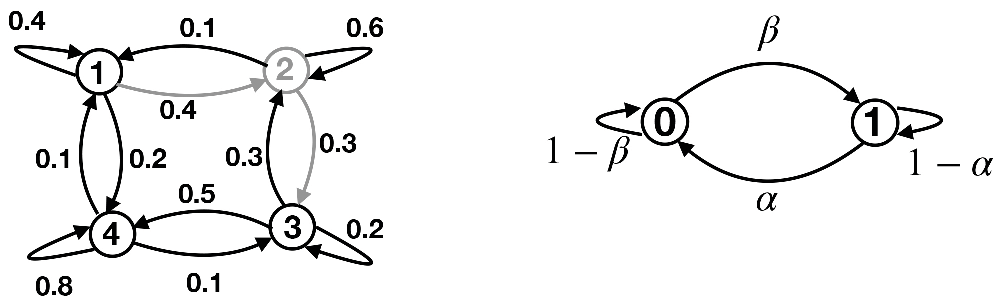
\includegraphics[width=1\textwidth]{ART_Majid/Markov-bw.pdf}\]
\caption{Markov process state diagrams on vertex set $X$ with transition probabilities labelling arrows of an extended graph. Associated functions on the left are $p=(0.6,0.4,0.8,0.2), q=(0.2,0.7,0.4, 0.7)$ in vertex order as numbered. 
\label{figmarkov}}
\end{figure}

We can go further and extend the geometric meaning of a Markov process by tropicalisation, i.e., by writing 
\[ p_{x\to y}= e^{-\lambda_{x\to y}},\quad p(x)=e^{-\lambda_{x\to x}},\quad \lambda_{x\to y}, \lambda_{x\to x}\ge 0\]
and observe that the transition probability after $n$-steps is
\[ P^n_{x,y}=\sum_{\gamma: x\to \cdots\to y} e^{- \lambda(\gamma)};\quad \lambda(\gamma)=\sum_{i=0}^{n-1}\lambda_{x_i\to x_{i+1}}\]
where $\gamma=x_0\to x_1\cdots \to x_{n-1}\to x_n$ is an $n$-step path from $x_0=x$ to $x_n=y$ (in the extended graph where we allow self-steps). If we think of $\lambda_{x\to y}$ as some kind of more geometric `asymmetric length' associated to the arrow or self-arrow then $\lambda(\gamma)$ is the `length' of the path $\gamma$. Thus we see how a generalised form of Riemannian geometry emerges as an interpretation of a Markov process, or conversely how Markov processes emerge naturally from generalised Riemannian geometry, with a contribution of maximal probability equated to a path of shortest length. It is generalised in the sense that `lengths' are direction dependent; there is no assumption that $\lambda_{x\to y}=\lambda_{y\to x}$ or even that one is nonzero when the other is, and we also allow self-arrow lengths $\lambda_{x\to x}$. Figure~\ref{figmarkov} shows the shortest path in this sense between 1 and 3 as via 2. In fact the generalised geometry here
is equivalent to the notion of a Lawvere metric space \parencite{ApCat} on the vertex set, where $d(x,y)$ is the length of the shortest path. The main difference is that in that context one would have $\lambda_{x,x}=0$ whereas in our case these are determined by the values on the arrows of the unextended graph. But in both cases, the self-arrow carries no new information and the actual data is the same. Moreover, this difference does not affect the shortest length provided these are all $\ge 0$, which {\em is} a restriction on the unextended graph weights in our case. In other words, we are not {\em not quite} freely labelling the arrows by lengths $\lambda_{x\to y}$ as there is a restriction
\[ \sum_{y: x\to y} e^{-\lambda_{x\to y}}\le 1\]
at every vertex. This has the character of some kind of lower bound on the `distances' from every vertex except that it is not one minimum e.g. Planck length, but shared between all local directions. Our observations may also be related to path integration defined by stochastic processes, even though our starting point is a fresh one. 


Finally, we consider if there is a Schr\"odinger version of a Markov process. We recall that in usual quantum mechanics, if $\psi$ obeys $\dot\psi= ({\imath\hbar\over 2 m}\Delta+ {V\over \imath\hbar})\psi$ and normalisation $||\psi||_{L^2}=1$ then the probability density $f=|\psi|^2$ obeys the conservation law
\[ \dot f+ \nabla\cdot J=0,\quad J=-{\imath\hbar\over 2m}(\bar\psi\nabla\psi - \psi \nabla\bar\psi)\]
where $J$ is the probability current. This implies that $\int \dot f=0$ so that $\int f=1$ holds at all times. Also note the formal similarity of the Schr\"odinger equation to an `imaginary time' (Wick rotation) version of the diffusion one.

We first compute in general that if we are on an inner $*$-differential algebra with $V=V^*\in A$, $\theta^*=-\theta$ and $*(\ ,\ )={\rm flip}(*\tens *)$ and set $f=\psi^*\psi$ as dependent on an additional continuous time with 
\[ \dot\psi=\imath(-\Delta_\theta+ V)\psi=\imath (\extd\psi,\theta)+\imath V\psi=-\imath(\theta,\extd\psi)+\imath[(\theta,\theta),\psi]+\imath V\psi\]
then
\[ \dot \psi^*=\imath(\theta,\extd \psi^*)-\imath \psi^*V\]
so that 
\[ \dot f=\dot\psi^*\psi+\psi^*\dot\psi=\imath(\theta,\extd \psi^*)\psi-\imath\psi^*(\theta,\extd\psi)+\imath\psi^*[(\theta,\theta),\psi].\]
If $A$ is commutative then this reduces to 
\[ \dot f=-(\ ,\ )(\theta\tens J)=-\nabla_\theta\cdot J,\quad J=\imath\left((\extd\psi)\psi^*-(\extd\psi^*)\psi\right)\]
as the probability current 1-form, where $\nabla_\theta=\theta\tens$ is the canonical connection. This remark only applies to continuous time, and moreover we do not necessarily have $\int:A\to \R$ specified, and even if we did, we may not have $\int \nabla_\theta\cdot J=0$ for all $\psi$. In case of an honest quantum metric and QLC, we might expect that $\int$ can be chosen depending on the metric so that integral of a divergence does vanish as in Riemannian geometry (it is not clear how generally we could do this). However, in our asymmetric setting, this seems unlikely both mathematically and physically; we should not expect actual conserved probability, but rather we have a formal similarity as well as an element of irreversibility. A partial result at our graph theory level is the following.

\begin{proposition}\label{propsch} Let $\psi_i\in \mathbb{C}(X)$ be complex valued, $V\in \R(X)$ real valued, $f_i=|\psi_i|^2$ and suppose that
\[ \del_+\psi = \imath(-\Delta_\theta + V)\psi, \]
where $\del_+$ acts on the discrete time index $i$. Then
\[ \del_+ f= V(-\Delta_\theta +V)f+ V(\extd\bar\psi,\extd \psi)-\nabla_\theta\cdot J,\]
\[ J=\imath((\extd\psi)\bar\psi-(\extd\bar\psi)\psi)-{1\over 2}((\extd\psi)\Delta_\theta\bar\psi+(\extd\bar\psi)\Delta_\theta\psi)\]
which we can also write as
\[\del_+ f = V^2 f-\nabla_\theta\cdot J_V,\]
\[ J_V=\imath((\extd\psi)\bar\psi-(\extd\bar\psi)\psi)+(\extd\psi)(-{1\over 2}\Delta_\theta+V)\bar\psi+(\extd\bar\psi)(-{1\over 2}\Delta_\theta+V)\psi.\]
\end{proposition}
\proof Here $-\Delta_\theta \psi=(\extd\psi,\theta)$ etc., so 
\[ \psi^{new}=\psi+ \imath((\extd\psi,\theta)+V\psi),\quad \bar\psi^{new}=\bar\psi- \imath((\extd\bar\psi,\theta)+V\bar\psi),\]
\begin{align*}
f^{\rm new}&=(\bar\psi- \imath((\extd\bar\psi,\theta)+V\bar\psi))(\psi+ \imath((\extd\psi,\theta)+V\psi))\\
&=f+ ((\extd\bar\psi,\theta)+V\bar\psi)((\extd\psi,\theta)+V\psi) + \imath \bar\psi (\extd\psi,\theta)- \imath(\extd\bar\psi,\theta)\psi\\
&=(1+V^2)f+ (\extd\bar\psi,\theta)(\extd\psi,\theta)+ (\extd\psi,\theta)(\imath+ V)\bar\psi\\
&\qquad\qquad + (\extd\bar\psi,\theta)(-\imath+V)\psi
\end{align*}
with a cross term $V\bar\psi\psi$ cancelling. Next
\[ (\extd \bar\psi,\theta)\psi=(\extd\bar\psi,\theta\psi)=(\extd\bar\psi,\extd\psi)+(\extd\bar\psi,\psi \theta)= (\extd\bar\psi,\extd\psi)+((\extd\bar\psi)\psi, \theta)\]
so this combined with $\bar\psi(\extd \psi,\theta)=(\bar\psi\extd \psi,\theta)$ contributes $V(\extd f,\theta)+ V(\extd\bar\psi,\extd\psi)$ to $f^{new}$. We also note that
\[- (\theta, (\extd\psi)\bar\psi- (\extd\bar\psi)\psi)= - (\theta,\extd\psi)\bar\psi+(\theta,\extd\bar\psi)\psi=(\extd\psi,\theta)\bar\psi-(\extd\bar\psi,\theta)\psi\]
which times $\imath$ verifies the first term of $J$. It remains to note that
\[ -(\theta,(\extd\bar\psi)(\extd\psi,\theta))=-(\theta,(\extd\psi)(\extd\bar\psi,\theta))=(\extd\bar\psi,\theta)(\extd\psi,\theta)\]
which times 1/2 for each expression as in $J$ gives the remaining term needed for $f^{new}$. This gives our first expression for $\del_+f=f^{new}-f$. For the second expression, we note that
\begin{align*}
-(\theta, (\extd\bar\psi)V\psi+(\extd\psi)V\bar\psi)=&V\bar\psi(\extd\psi,\theta)\\
&+V\psi(\extd\bar\psi,\theta)=V(\extd f,\theta)+V(\extd\bar\psi,\extd\psi)
\end{align*}
%\[ -(\theta, (\extd\bar\psi)V\psi+(\extd\psi)V\bar\psi)=V\bar\psi(\extd\psi,\theta)+V\psi(\extd\bar\psi,\theta)=V(\extd f,\theta)+V(\extd\bar\psi,\extd\psi)\]
as required for the extra terms in $J_V$ to replace the corresponding terms in $f^{new}$. \endproof

Writing 
\[ J=\sum_{x\to y}J_{x\to y}\omega_{x\to y},\quad \tilde\psi(y)=\sum_{y:x\to y}\psi(y)p_{y\to x},\]
explicit formulae for the various terms are
\begin{align*}
(\extd\bar\psi,\extd\psi)(x)=&-\sum_{y:x\to y}f(y)p_{y\to x}- f(x)q(x)\\
&+\sum_{y:x\to y}(\psi(x)\bar\psi(y)+\bar\psi(x)\psi(y))p_{y\to x}
\end{align*}
%\[ (\extd\bar\psi,\extd\psi)(x)=-\sum_{y:x\to y}f(y)p_{y\to x}- f(x)q(x)+\sum_{y:x\to y}(\psi(x)\bar\psi(y)+\bar\psi(x)\psi(y))p_{y\to x}\]

\begin{align*} &\scalemath{0.99}{J_{x\to y}=\imath(\psi(y)\bar\psi(x)- \bar\psi(y)\psi(x))+ {1\over 2}\Big(\psi(y)\bar{\tilde\psi}(x)+\bar\psi(y)\tilde\psi(x)}\\
&\scalemath{0.99}{-\psi(x)\bar{\tilde\psi}(x) -\bar\psi(x)\tilde\psi(x)
-(\psi(y)\bar\psi(x)+\bar\psi(y)\psi(x))q(x)\Big)+ f(x)q(x)}\end{align*}
and the additional terms in $J_V{}_{x\to y}$ are
\[ V(x)(\psi(y)\bar\psi(x)+\bar\psi(y)\psi(x)-2f(x)). \]
A direct calculation from $f^{new}$ in the proof above also gives:

\begin{proposition} For the discrete Schr\"odinger process $\del_+\psi=\imath(-\Delta_\theta+V)\psi$, we have 
%\begin{align*}
%\sum_X \del_+ f=\sum_X\left( &(V-q)^2 f+ (V-q)(\bar\psi\tilde\psi+\bar{\tilde{\psi}}\psi)\\
%&+ |\tilde\psi|^2+\imath(\bar\psi\tilde\psi-\bar{\tilde{\psi}}\psi) \right)
%\end{align*}
\[\scalemath{0.95}{ \sum_X \del_+ f=\sum_X\left((V-q)^2 f+ (V-q)(\bar\psi\tilde\psi+\bar{\tilde{\psi}}\psi)+ |\tilde\psi|^2+\imath(\bar\psi\tilde\psi-\bar{\tilde{\psi}}\psi)\right)}\]
for $f=|\psi|^2$. 
\end{proposition}

This is typically not zero, i.e. the discrete Schr\"odinger process with the $\nabla_\theta$ connection does not leave the $l^2$-norm $\sum_x |\psi|^2$ constant, i.e. does not consist of unitary steps. This is visible even for $V=q$, when $\del_+\psi=\imath\tilde\psi$, and is due in part to the 1-sided step $\del_+f$ not reflecting a $*$-calculus on $\Z$. It is also due to the connection $\nabla_\theta$ being a convenient but not necessarily physical choice. Nevertheless, we see from the proposition that $\del_+f$ has a certain form which, when $V=0$, is $\del_+ f=-\nabla_\theta\cdot J$ as expected in quantum mechanics from a formal point of view, while for other $V$ also contains a Markov-process like element. 

More generally, we should consider the discrete Schr\"odinger process with other bimodule connections $\nabla$ on $\Omega^1$ and the associated $\Delta$ and $\nabla\cdot$ from (\ref{divlap}). We will say that a connection $\nabla$ is {\em unitary} if there exists a potential $V$ such that $\del_+\psi =\imath(-\Delta+V)\psi$ indeed has unitary steps so that the total probability is conserved. In the remainder of this section, we explore this idea for the simplest example of a two state process. 

\begin{example} Let $X=\{0,1\}$ with $\alpha=p_{1\to 0}>0$ and $\beta=p_{0\to 1}>0$ define a classical 2-state Markov process as shown on the right in Figure~\ref{figmarkov}. In addition to this process interpreted as in Proposition~\ref{propmar} in terms of $\nabla_\theta$, we consider the same ideas as in Proposition~\ref{propsch} but for Laplacian and divergence given by a general bimodule connection $\nabla$. It is known from \parencite[Lemma~2.1]{Ma:squ} that these take the form
\[ \nabla\theta= (1-b)\theta\tens\theta,\quad b(0)=s,\quad b(1)=t\]
for two complex parameters $s,t$. Here, $\theta= \omega_{0\to 1}+\omega_{1\to 0}$ is a basis over the algebra, so it is enough to specify $\nabla$ on this. Its general value deduced from the Leibniz rule
\[ \nabla(\psi\theta)=\extd \psi\tens\theta+\psi\nabla\theta;\quad \extd \psi=(\psi(1)-\psi(0))(\omega_{0\to 1}-\omega_{1\to 0})\]
comes out as
\begin{equation}
\begin{gathered}
\label{nablas} \nabla\omega_{0\to 1}=\omega_{1\to 0}\tens\omega_{0\to 1}-s\omega_{0\to 1}\tens\omega_{1\to 0},\\
\nabla\omega_{1\to 0}=\omega_{0\to 1}\tens\omega_{1\to 0}-t\omega_{1\to 0}\tens\omega_{0\to 1}.
\end{gathered}
\end{equation}
Meanwhile, the metric inner product is
\[ (\omega_{0\to 1},\omega_{1\to 0})=\alpha\delta_0,\quad (\omega_{1\to 0},\omega_{0\to 1})=\beta\delta_1\]
and it is known also from \parencite[Lemma~2.1]{Ma:squ} that $\nabla$ is metric compatible (and hence a QLC for the standard exterior algebra) if and only if $\beta=\pm\alpha$, which in our context means $\beta=\alpha$, and $t=s^{-1}$. Moreover, in this case it is $*$-preserving if and only if $s$ has modulus 1. So there is a circle of $*$-preserving QLCs, including the obvious $s=t=-1$ with $\nabla\theta=2\theta\tens\theta$. By contrast, the canonical one we studied above was $\nabla_\theta \theta=\theta\tens\theta$ at $s=t=0$. 

We proceed with a general bimodule connection (\ref{nablas}) for our discussion, remembering that it is a QLC only when $\beta=\alpha$ and $s=t^{-1}$. The metric inner product is
\[ (\omega_{0\to 1},\omega_{1\to 0})=\alpha\delta_0,\quad (\omega_{1\to 0},\omega_{0\to 1})=\beta\delta_1\]
so that the Laplacian comes out as as
\[ \scalemath{0.93}{(\Delta\psi)(0)=-\delta_\psi\alpha(1+s),\quad (\Delta\psi)(1)=\delta_\psi \beta(1+t);\quad \delta_\psi:=\psi(1)-\psi(0).}\]
The discrete Schr\"odinger process $\del_+\psi=\imath(-\Delta+V)\psi$ then corresponds to the matrix step on the column vector $\psi(0),\psi(1)$,
\[\begin{gathered}
\psi^{new}=U\psi;\\
\quad U= \begin{pmatrix} 1+\imath V(0) -\imath\alpha(1+s) & \imath\alpha(1+s)\\ \imath\beta(1+t) & 1+ \imath V(1) - \imath\beta(1+t)\end{pmatrix},
\end{gathered} \]
which is unitary if and only if 
\[\begin{gathered}
\imath\alpha(1+s)=-e^{\imath\phi}\bar z,\quad |1+\imath V(1) - z |^2+ |z|^2=1,\\
\quad 1+ \imath V(0)=-e^{\imath\phi}(2 \bar z - 1+\imath V(1)),
\end{gathered}  \]
where $z=\imath\beta(1+t)$ and $e^{\imath\phi}$ is some phase. This has solution 
\begin{equation}\label{solphi}\begin{gathered}
V(0)=V(1)=0,\quad z={1\over 2}(1-e^{\imath\phi}),\\
s=-1-{\imath\over 2\alpha}(1-e^{\imath\phi}),\quad t=-1-{\imath\over 2\beta}(1-e^{\imath\phi})
\end{gathered}\end{equation}
for a free angle parameter $\phi$, with resulting Schr\"odinger process step
\begin{equation}\label{Uphi} U=\begin{pmatrix}
 1-z & z \\
 z& 1-z \\
\end{pmatrix}
=e^{\imath\phi\over 2}\begin{pmatrix}
 \cos({\phi\over 2}) & -\imath\sin({\phi\over 2})\\ -\imath\sin({\phi\over 2}) & \cos({\phi\over 2}) 
\end{pmatrix}.\end{equation}
{\em Thus, the 2-point graph has a 1-parameter circle of bimodule connections $\nabla$ which are `unitary' in the sense that the step operator $U$ is unitary.} Some examples are:

(i) $\phi=0$ or $z=0$ gives $s=t=-1$ in the QLC family and
\[ \nabla\theta=2\theta\tens\theta,\quad U=\id;\]

(ii) $\phi=\pi$ or $z=1$  gives $s=-1-{\imath\over \alpha}$ and $t=-1-{\imath\over \beta}$ and
\[ \nabla\theta=(2+{\imath \over \gamma})\theta\tens\theta;\quad \gamma(0)=\alpha,\quad \gamma(1)=\beta;\quad U=\begin{pmatrix}0&1\\1&0\end{pmatrix}.\]
By contrast, our canonical $\nabla\theta=\theta\tens\theta$ at $s=t=0$ is not on this circle. 

\begin{proposition} For the 1-parameter circle of unitary discrete Schr\"odinger evolutions (\ref{solphi})--(\ref{Uphi}), and writing $f=|\psi|^2$ in vector notation, we find
\begin{align*}
f^{new}=&\begin{pmatrix} \cos^2({\phi\over 2}) & \sin^2({\phi\over 2})\\ \sin^2({\phi\over 2}) & \cos^2({\phi\over 2})\end{pmatrix}f\\ &\qquad+{\imath\over 2}\sin(\phi) \left(\bar\psi(0)\psi(1)-\bar\psi(1)\psi(0)\right)\begin{pmatrix}-1\\ 1\end{pmatrix}.
\end{align*}
The first term is a general left and right stochastic Markov process on $f$. In quantum geometric terms,
\[\begin{gathered}
\del_+\psi= -\imath\Delta\psi,\quad \del_+f={1\over 2\imath}(1-e^{-\imath\phi})\Delta f- \nabla\cdot J,\\
J={\imath\over 2} (1+e^{-\imath\phi})\left((\extd\psi)\bar\psi-(\extd\bar\psi)\psi\right). 
\end{gathered} \]
\end{proposition}
\proof Here 
\begin{align*} f^{new}(0)&=|\psi^{new}(0)|^2=|(1-z)\psi(0)+z\psi(1)|^2\\
&=|1-z|^2f(0)+|z|^2f(1)+(1-\bar z)z\bar\psi(0)\psi(1)\\
&\qquad\qquad + \bar z(1-z)\bar\psi(1)\psi(0)\\
&=\cos^2({\phi\over 2})f(0)+ \sin^2({\phi\over 2})f(1)- {\imath\over 2}\sin(\phi)(\bar\psi(0)\psi(1)\\
&\qquad\qquad -\bar\psi(1)\psi(0))\end{align*}
and similarly for $f^{new}(1)=|\psi^{new}(1)|^2=|(1-z)\psi(1)+z\psi(0)|^2$. Note that the entries of $f$ remain positive and summing to 1 even though there is an extra divergence term. 

We next consider a general 1-form $J=J_{01}\omega_{0\to 1}+J_{10}\omega_{1\to 0}$ for constants $J_{01},J_{10}$ and find from (\ref{nablas}) and (\ref{solphi}) that
\begin{align*}\nabla\cdot J&= (\ ,\ )\big(J_{01}(\omega_{1\to 0}\tens\omega_{0\to 1}- s\omega_{0\to 1}\tens\omega_{1\to 0})\\
&\qquad+ J_{10}(\omega_{0\to 1}\tens\omega_{1\to 0}- t\omega_{1\to 0}\tens\omega_{0\to 1})\big)\\
&=(J_{10}-sJ_{01})\alpha \delta_0+ (J_{01}-t J_{10})\beta\delta_1\\
&=(J_{01}+J_{10})\gamma+ {\imath\over 2}(1-e^{\imath\phi})j\end{align*}
where $\gamma(0)=\alpha, \gamma(1)=\beta$ and $j(0)=J_{01}, j(1)=J_{10}$ are functions on $X$. If we set $J_{01}=-J_{10}={\imath\over 2}(1+e^{-\imath\phi})(\bar\psi(0)\psi(1)-\bar\psi(1)\psi(0))$ then $-\nabla\cdot J$ gives the second term of $f^{new}$ as required. This gives $J$ as stated after we observe that
\begin{align*} (\extd\psi)\bar\psi-(\extd\bar\psi)\psi&=(\psi(1)-\psi(0))(\omega_{0\to 1}-\omega_{1\to 0})\bar\psi\\
&\quad-(\bar\psi(1)-\bar\psi(0))(\omega_{0\to 1}-\omega_{1\to 0})\psi\\
&=(\psi(1)-\psi(0))\bar\psi(1)\omega_{0\to 1}-(\psi(1)-\psi(0))\bar\psi(0)\omega_{1\to 0}\\
&\quad-(\bar\psi(1)-\bar\psi(0))\psi(1)\omega_{0\to 1}+(\bar\psi(1)-\bar\psi(0))\psi(0)\omega_{1\to 0}\\
&=(\bar\psi(0)\psi(1)-\bar\psi(1)\psi(0))(\omega_{0\to 1}-\omega_{1\to 0}).\end{align*}


Moreover, $\extd f=(f(1)-f(0))(\omega_{0\to 1}-\omega_{1\to 0})$. Hence, using our computation of $\nabla\cdot$, 
\begin{align*}
\Delta f=\nabla\cdot\extd f&={\imath\over 2}(1-e^{\imath\phi})(f(1)-f(0))\begin{pmatrix}1\\-1\end{pmatrix}\\
&={\imath\over 2}(1-e^{\imath\phi})\begin{pmatrix}-1 & 1\\ 1 & -1\end{pmatrix}f
\end{align*}
in vector notation for $f$ (which, when applied to $\psi$, recovers the Schr\"odinger process step $U=1-\imath\Delta$ in (\ref{Uphi}) as expected). Moreover, the stated first term of $\del_+f$ is then
\[ {1\over 2\imath}(1-e^{-\imath\phi}){\imath\over 2}(1-e^{\imath\phi})\begin{pmatrix}-1 & 1\\ 1 & -1\end{pmatrix}f=\sin^2({\phi\over 2})\begin{pmatrix}-1 & 1\\ 1 & -1\end{pmatrix}f\]
as required in $f^{new}-f$. \endproof \end{example}

For the $l^2$-norm, we took the constant measure in summing over $X$. One could also, in principle, introduce a measure related to the quantum metric $(\ ,\ )$. This would be more in keeping with Riemannian geometry but is not so natural from our point of view on Markov processes (where the usual constant measure is preserved). 

\section{Digital geometry of $2\times 2$ matrices} \label{secM2}

Quantum Riemannian geometry and quantum gravity on one of the simplest graphs, a quadrilateral, was recently achieved \parencite{Ma:squ} (with Lorentzian style negative square-length weights on two of the sides). Here we briefly look at the complementary example of a noncommutative finite geometry, namely the humble algebra of $2\times 2$ matrices $M_2(\mathbb{C})$. Its quantum Riemannian geometry turns out to be rather rich and is not fully explored. 

We take the standard 2D $*$-differential calculus from \parencite{BegMa:spe, BegMa} with a basis of central 1-forms $s,t\in \Omega^1(M_2)$, differential and exterior algebra
\[\extd a= [E_{12},a]s+ [E_{21},a]t,\]
\[ s^2=t^2=0,\quad s\wedge t=t\wedge s,\quad \extd s=2\theta\wedge s,\quad\extd t=2\theta\wedge t,\quad s^*=-t,\]
which is inner with $\theta=E_{12}s+E_{21}t$. Here $E_{ij}$ is the matrix with $1$ in the $(i,j)$ place and 0 elsewhere. 

Next, as the basis is central and the metric has to be central to be invertible in the bimodule sense, any invertible $2\times 2$ complex matrix $g_{ij}$ in our basis can be taken as metric coefficients, with the condition that $g_{12}=-g_{21}$ if we want to impose quantum symmetry, and $g_{22}=\overline{g_{11}}$, $g_{12}$ real if we want $g$ to be `real' in the required hermitian sense. It is easy to see that
\begin{equation}\label{M2canQLC} \nabla s=2\theta\tens s,\quad \nabla t=2\theta\tens t,\quad \sigma=-{\rm flip},\quad R_\nabla=0\end{equation}
on the generators is a flat QLC simultaneously for all quantum metrics. But there are typically many more QLCs. The actual moduli of these has only been computed in \parencite[Example~8.13 and Exercise 8.3]{BegMa} for a couple of sample quantum metrics $g_1,g_2$, with results there as follows. 

(i) $g_1=s\tens t-t\tens s$. This has a principal 4-parameter moduli of QLCs of the form
\begin{align*}
\nabla s=&2\theta\tens s - \begin{pmatrix}0&\mu\alpha\\ \beta & 0\end{pmatrix}s\tens s -\begin{pmatrix}0&\alpha\\ \nu\beta & 0\end{pmatrix}g_1\\
& +\begin{pmatrix}0&\nu\alpha\\ \nu^2\beta+(\mu\nu-1)\alpha & 0\end{pmatrix}t\tens t,
\end{align*}
%\[ \nabla s=2\theta\tens s - \begin{pmatrix}0&\mu\alpha\\ \beta & 0\end{pmatrix}s\tens s -\begin{pmatrix}0&\alpha\\ \nu\beta & 0\end{pmatrix}g_1 +\begin{pmatrix}0&\nu\alpha\\ \nu^2\beta+(\mu\nu-1)\alpha & 0\end{pmatrix}t\tens t, \]
\begin{align*}
\nabla t=&2\theta\tens t+\begin{pmatrix}0&\mu^2\alpha+(\mu\nu-1)\beta\\ \mu\beta & 0\end{pmatrix}s\tens s\\
&+\begin{pmatrix}0&\mu\alpha\\ \beta & 0\end{pmatrix}g_1 - \begin{pmatrix}0&\alpha\\ \nu\beta & 0\end{pmatrix} t\tens t.
\end{align*}
%\[ \nabla t=2\theta\tens t+\begin{pmatrix}0&\mu^2\alpha+(\mu\nu-1)\beta\\ \mu\beta & 0\end{pmatrix}s\tens s+\begin{pmatrix}0&\mu\alpha\\ \beta & 0\end{pmatrix}g_1- \begin{pmatrix}0&\alpha\\ \nu\beta & 0\end{pmatrix} t\tens t.\]
The $\alpha=\beta=\mu=\nu=0$ point is the flat one (\ref{M2canQLC}). We rescaled the $\mu,\nu$ compared to \parencite{BegMa} here and in the next case. 

(ii) $g_2=s\tens s+ t\tens t$. This has a principal 3-parameter moduli of QLCs of the form
\begin{align*}
\nabla s=&2E_{21}t\tens s + \begin{pmatrix}0&\mu\rho\\ 2\mu-\rho(1+\mu(\mu+\nu)) & 0\end{pmatrix}s\tens s\\
& +\begin{pmatrix}0&-\rho \\ \mu\rho & 0\end{pmatrix}g_1 +\begin{pmatrix}0&\nu\rho\\ \rho & 0\end{pmatrix}t\tens t,
\end{align*}
%\[ \nabla s=2E_{21}t\tens s + \begin{pmatrix}0&\mu\rho\\ 2\mu-\rho(1+\mu(\mu+\nu)) & 0\end{pmatrix}s\tens s +\begin{pmatrix}0&-\rho \\ \mu\rho & 0\end{pmatrix}g_1 +\begin{pmatrix}0&\nu\rho\\ \rho & 0\end{pmatrix}t\tens t, \]
\begin{align*}
\nabla t=&2E_{12}s\tens t +\begin{pmatrix}0&- \rho\\ \mu\rho & 0\end{pmatrix} s\tens s -\begin{pmatrix}0&\nu \rho \\ \rho & 0\end{pmatrix}g_1\\
& +\begin{pmatrix}0& -2\nu+\rho(1+\nu(\mu+\nu))\\ \nu\rho & 0\end{pmatrix}t\tens t.
\end{align*}
%\[\nabla t=2E_{12}s\tens t +\begin{pmatrix}0&- \rho\\ \mu\rho & 0\end{pmatrix} s\tens s -\begin{pmatrix}0&\nu \rho \\ \rho & 0\end{pmatrix}g_1 +\begin{pmatrix}0& -2\nu+\rho(1+\nu(\mu+\nu))\\ \nu\rho & 0\end{pmatrix}t\tens t. \]
There are restrictions on the parameters over $\mathbb{C}$ for a $*$-preserving connection. The $\mu=\nu=\rho=0$ point has curvature
\[ R_\nabla s=2 s\wedge t\tens s,\quad R_\nabla t=2 s\wedge t\tens t.\]
We also have an obvious `symmetric lift' $i(s\wedge t)={1\over 2}( s\tens t+ t\tens s)$ which at the zero parameter point yields 
\[ {\rm Ricci}=s\tens t+t\tens s,\quad S=0,\]
but note that $i$ in the $*$-algebra case is not antihermitian in the required sense so that this Ricci is not hermitian.

The above are principal moduli with nontrivial $\sigma$ and zero for the bimodule map $\alpha$ in the general construction; there is also a 4 dimensional moduli of QLCs for $g_2$ with $\sigma=-{\rm flip}$. In general, the space of $*$-preserving `real' pairs $(g,\nabla)$ appears to be generically 7 dimensional, although this remains to be determined. Once known, one could define quantum gravity on $M_2(\mathbb{C})$ by integration over this moduli, schematically,
\[ \langle\mathbb{C}O_1\mathbb{C}O_2\rangle={\int\mathbb{C}D(g,\nabla) e^{\imath {\rm Tr} S[g,\nabla]}\mathbb{C}O_1\mathbb{C}O_2\over \int \mathbb{C}D(g,\nabla)e^{\imath {\rm Tr} S[g,\nabla]} } \]
for the given differential structure and lift $i$ fixed. Here $S[g,\nabla]\in M_2(\mathbb{C})$ is the Ricci scalar, which generically is expected not to vanish. One could also consider summing or integrating over the choice of differential structure up to diffeomorphism. 

It is natural to ask how this approach to quantum gravity compares to other, more established, approaches. A direct comparison is not possible due to very different methodologies, but taking the `coordinate algebra' finite dimensional as we did above is broadly in the spirit of replacing spacetime by a finite geometry, such as a finite lattice or triangulation \parencite{AJL}. A main difference in our case is that we approach the matter in a coherent way that applies, as we saw in Section~\ref{secqg}, to general algebras including finite-dimensional ones at one end of the range and classical $C^\infty(M)$ for a manifold $M$ at the other, without too many ad-hoc steps. A consequence is that one can in principle take a limiting process from one to the other without ever leaving the category of models. Thus, the polygon lattice $\Z_n$ in \parencite{ArgMa} with its 2D calculus can be seen in the limit $n\to\infty$ to tend to $S^1$ with a certain 2D calculus. This turns out to be a central extension of the classical calculus on a circle in the sense of \parencites{Ma:rec}[Chapter~8.3]{BegMa}, where the `partial-derivative' associated to the extra dimension is a 2\textsuperscript{nd} order Laplacian-like operator giving something like an Ito derivative in stochastic calculus. Here, the polygon graph is viewed as bidirected $i\leftrightarrow i+1$ at vertices numbered in sequence mod $n$, and this is the reason for the 2D calculus. As we have seen in Section~\ref{secmarkov}, we can also work with 1-way arrows $x\to y$, and this could make contact with causal set models \parencite{Dow} where $x\to y$ indicates a causal path between spacetime points. So far in quantum Riemannian geometry models, the Lorentzian case has been handled by having `square-length' weights $<0$ on designated timelike edges \parencite{Ma:squ}. In such models, one could think of the causal structure as a choice of orientation of the subgraph of timelike edges (choosing an arrow direction for each such edge).

Other approaches such as loop quantum cosmology \parencite{Ash} also drastically cut the degrees of freedom to the point of computability. From such models as well as from experience with 2+1 quantum gravity, it does appear that some quantum gravity effects could be modelled by a noncommutative spacetime, which is support for our underlying framework. What we would hope for here is a kind of `eigengeometry' where quantum gravity effects render spacetime noncommutative as a better approximation than classical, then quantisation of gravity on that background results in effects which justify the supposed quantum spacetime as the effective background. This is a circular self-consistency condition, the content of which has yet to be understood. There have also been attempts at discrete quantum gravity in Connes' spectral triple approach to noncommutative geometry, where one integrates over possible Dirac operators \parencite{Hal} on $\Z_2$. Although very different, the results are not unlike the those of \parencite{Ma:squ,ArgMa} in that there is a constant relative uncertainty. This work also looks at integration over spectral triples on $M_2(\mathbb{C})$.

Next, what about the landscape of {\em all} finite quantum Riemannian geometries of small algebra dimension? This is a tough classification programme and so far has been achieved \parencite{MaPac2} only up to dimension 3 and by specialising to the digital case over the field $\F_2=\{0,1\}$ to simplify the problem. Here algebra dimension 2 has no interesting quantum geometries, while for dimension 3 there are 7 algebras labelled A--G but only B,D,F admit quantum Riemannian geometries, as summarised in the table in Figure~\ref{figtab}. Here B is the Boolean algebra of subsets of a set of three elements with calculus and metric corresponding to an equilateral triangle graph, forming the group $\Z_3$. It is a Hopf algebra and its dual is the group algebra D$=\F_2\Z_3$. Its three quantum metrics are related by an overall element of the algebra (i.e., `conformally equivalent' in some sense). In each case, the 4 QLCs with 1 flat and 3 nonflat is the opposite of what was found for $B$, possibly consistent with Hopf algebra duality interchanging high and low curvature \parencite[cf.][]{Ma:pla,Ma:pri}. For $\F_8$, the 7 metrics are again related by invertible factors but fall into three groups behaving differently as shown in the table. Details of the connections and curvatures are given in \parencite{MaPac2}. 

\begin{figure}
\[ 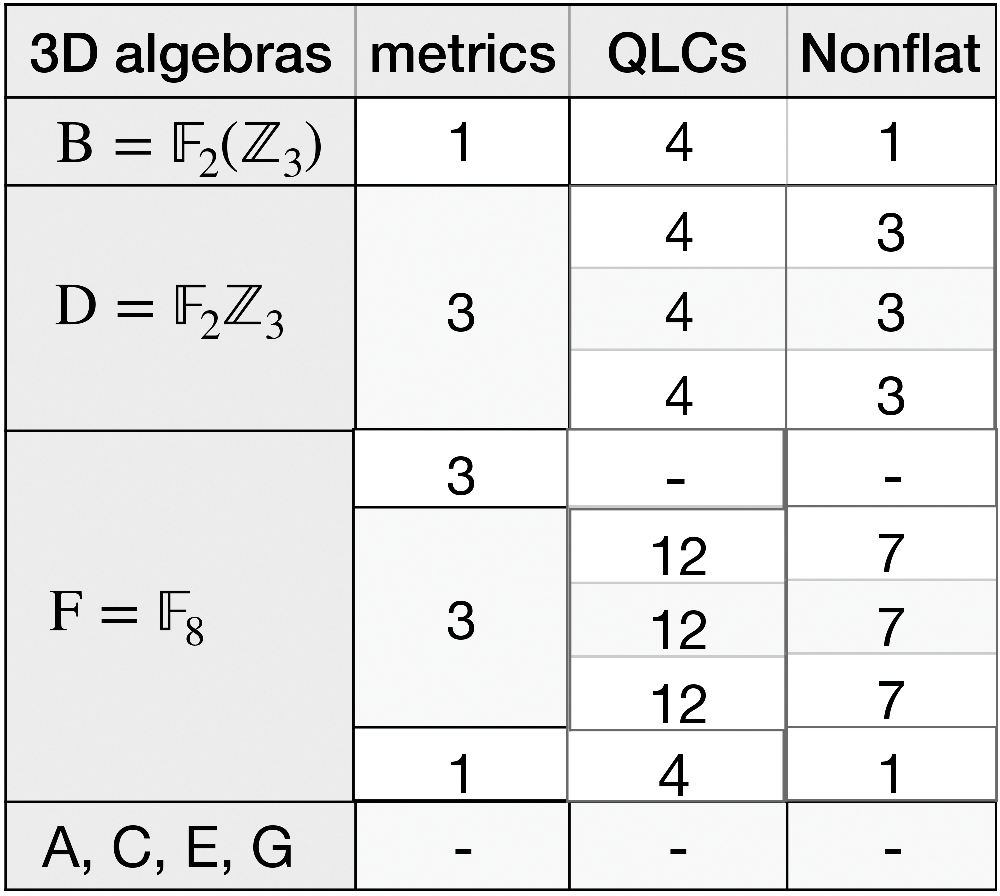
\includegraphics[width=.5\textwidth]{ART_Majid/table-bw.pdf}\]
\caption{Number of quantum geometries over $\F_2$ of algebra dimension 3 and 2D parallelisable calculus $\Omega$. Data from \parencite{MaPac2}. 
\label{figtab}}
\end{figure}


For interesting examples with the algebra noncommutative, we therefore need to go to dimension $n=4$, which was beyond the computer power available when writing \parencite{MaPac2} (where QLCs were found by trying some $2^{24}$ possible connection values). As a result, the landscape of all quantum geometries for $n=4$ is largely unexplored, though some flat connections are known for the algebra $A_2$ in the family of Hopf algebras over $\F_2$ in \parencite{BasMa}. In dimension 4, there are 9 distinct noncommutative algebras \parencite{MaPac3} (and 16 commutative ones) over $\F_2$, and one of the former is of course $M_2(\F_2)$. 

Here we note that by reducing the above generic solutions for $M_2(\mathbb{C})$ to the $\F_2$ case, we can obtain some, though not necessarily all, of the quantum geometries on $M_2(\F_2)$, at least for the two metrics stated above. Since 2=0 in $\F_2$, we now have $\extd s=\extd t=0$, and indeed $t=\extd E_{12}$, $s=\extd E_{21}$ are exact. Setting the parameters for our generic solutions to all values 0,1 gives us up to 16 and 8 QLCs respectively for our standard metrics, which appear now as
\[ g_1=s\tens t+t\tens s,\quad g_2=s\tens s+ t\tens t.\]
We broadly identify four cases: 

(a) Setting $\alpha=\beta=\rho=0$ and any $\mu,\nu$ gives the zero flat QLC $\nabla s=\nabla t=0$ for both metrics. 

(b) Setting $\alpha=\beta=\rho=1$ and $\mu=\nu=1$ gives another flat QLC 
\[ \nabla s=\nabla t= \sigma_1(g_1+g_2),\quad R_\nabla=0\]
for both metrics, on noting that $\nabla (s+t)=0$. Here $\sigma_1=E_{12}+E_{21}$. 

(c) Setting $\alpha=\beta=\rho=1$ and $\mu=\nu=0$ gives another flat QLC 
\[ \nabla s=E_{12}g_1+ E_{21} g_2,\quad \nabla t=E_{21}g_1+ E_{12} g_2,\quad R_\nabla=0\]
for both metrics, on noting that $\extd(E_{12}t)=\extd(E_{21}s)=0$ and $\extd(E_{12}s)=\extd(E_{21}t)=s\wedge t$. 

\begin{figure}[h]
\[ 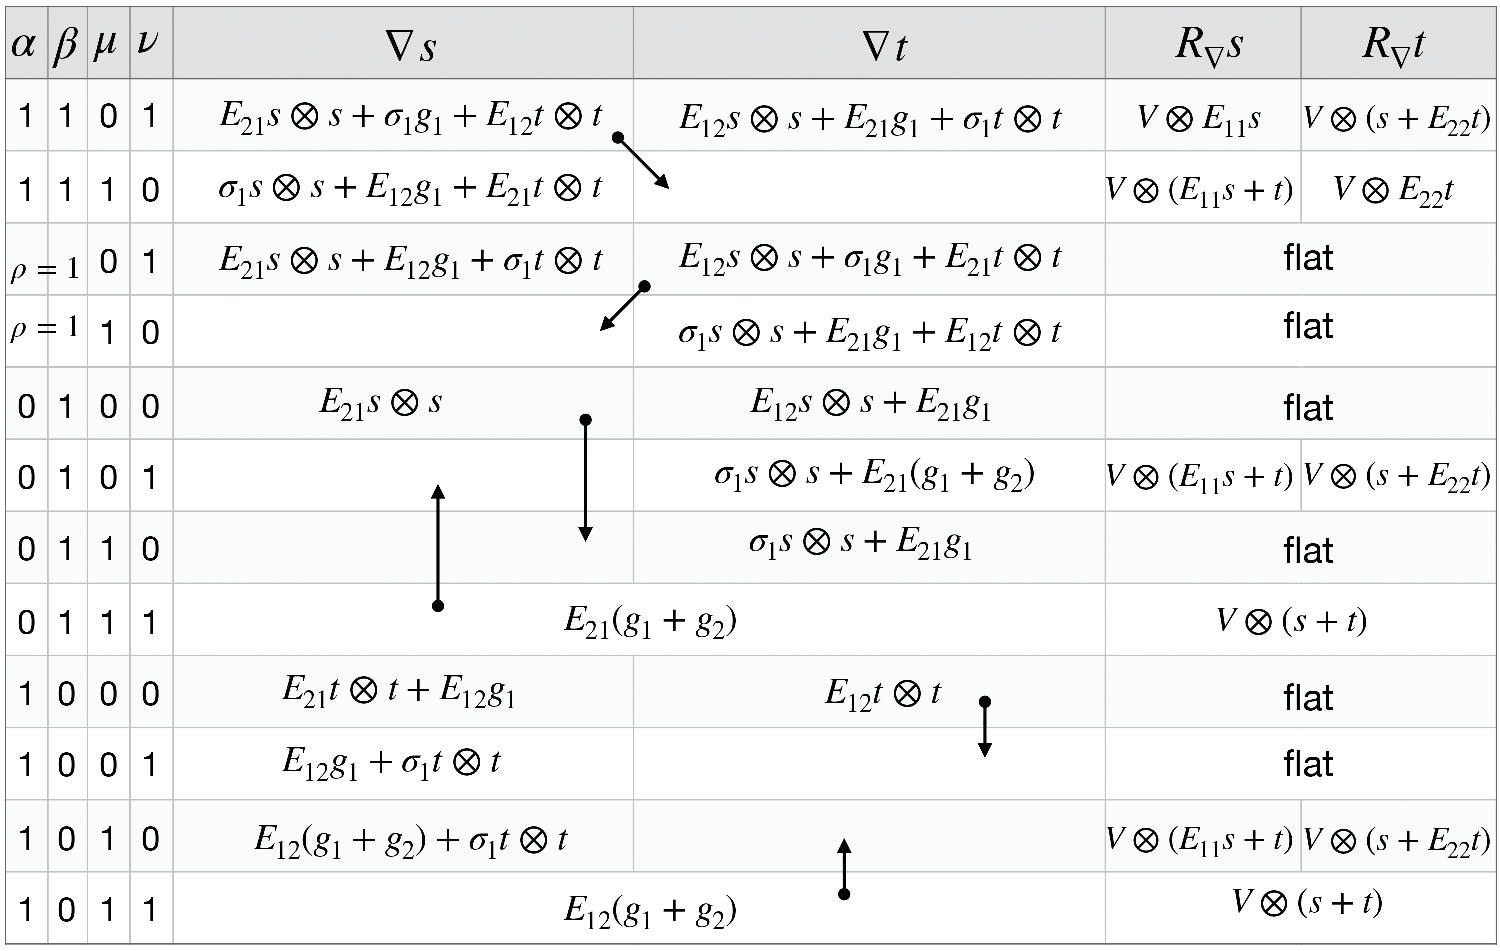
\includegraphics[width=1\textwidth]{ART_Majid/curvtab-bw.pdf}\]
\caption{All QLCs on $M_2(\F_2)$ arising as limits of connections over $\mathbb{C}$ (which may not be all of them). All are for $g_1$ except the $\rho=1$ rows for $g_2$, which are flat. We see 6 with curvature, where $V=s\wedge t$ is the `volume form'. 
\label{figtab2}}
\end{figure}

(d) For curvature, we therefore need to look to $\alpha\ne \beta$ or $\mu\ne \nu$. These are shown in the table Figure~\ref{figtab2}, where we see that half of them have Riemann curvature, all QLCs for the metric $g_1$. 

Next, the usual lift $i$ needed for the Ricci curvature, and the Einstein tensor, both present a problem over $\F_2$ in that there is no $1/2$ at our disposal. Our approach in \parencite{MaPac2} is to look at all possible $i$ and tentatively to define ${\rm Eins}={\rm Ricci}+g S$. Now we explore a different idea which is not systematic but applies when the exterior algebra has a suitable form, namely to look for two halves of the classical `antisymmetric' lifts' separately, without the factor $1/2$. For the $M_2(\F_2)$ calculus as above, obvious choices would be
\[ i_+(s\wedge t)= s\tens t,\quad i_-(s\wedge t)= t\tens s.\]
As a result, there are two natural Ricci tensors ${\rm Ricci}_\pm$ as defined with $i_\pm$. If $S_+=S_-=S$, i.e., if the two Ricci scalars are the same then we propose
\[ {}_2{\rm Ricci}= {\rm Ricci}_++{\rm Ricci}_-,\quad {}_2{\rm Eins}={}_2{\rm Ricci}+ g S\]
For the 3-dimensional Boolean algebra B, this gives ${}_2{\rm Ricci}=g$, $S=1$ and ${}_2{\rm Eins}=0$ but for the D algebra one has $S_+\ne S_-$ for the obvious lifts (which is not to say the new approach could not work, for suitable $i_\pm$.) 


\begin{proposition} On $M_2(\F_2)$ with the metric $g_1$ as above and its two nonflat joint QLCs in Figure~\ref{figtab2} with curvature $R_\nabla s=R_\nabla t=s\wedge t\tens (s+t)$, we have
\[\begin{gathered}
{\rm Ricci}_+=t\tens (s+t),\quad {\rm Ricci}_-=s\tens (s+t),\quad S_\pm=1;\\ {}_2{\rm Ricci}=g_1+g_2,\quad {}_2{\rm Eins}=g_2.
\end{gathered}  \]
Moreover, $\nabla$ here are also QLCs for $g_2$ and hence $\nabla( {}_2{\rm Ricci})=\nabla ({}_2{\rm Eins})=0$. 
The three other types of curvature for QLCs of $g_1$ in Figure~\ref{figtab2} have $S_+\ne S_-$. 
\end{proposition}
\proof We use the curvature as shown and take the `trace' with respect to $g_1$ as this is the relevant metric. Since the output of $R_\nabla$ is the same on $s,t$, 
\[ {\rm Ricci}_+=((s+t ,\ )\tens\id)( s\tens t\tens (s+t))=t\tens (s+t),\quad S_+=1,\]
\[ {\rm Ricci}_-=((s+t ,\ )\tens\id)( t\tens s\tens (s+t))=s\tens (s+t),\quad S_-=1.\]
In this case, we also have ${}_2{\rm Ricci}=(s+t)\tens (s+t)=g_1+g_2$ on adding these. Hence adding $Sg_1$ gives us the other metric. We next look more closely at the two connections in the table with this curvature. The one on the bottom line at $\alpha=\mu=\nu=1$ and $\beta=0$ has braiding
\[\sigma( \begin{cases}s\\ t\end{cases}\nquad\tens s)=s\tens \begin{cases}s\\ t\end{cases}\nquad+ g_1+g_2,\quad \sigma(\begin{cases}s\\ t\end{cases}\nquad\tens t)=t\tens \begin{cases}s\\ t\end{cases}\nquad.\]
Then since $\nabla$ has the same value on $s,t$, 
\begin{align*}\nabla g_2&=\nabla s\tens s+\nabla t\tens t+(\sigma\tens\id)(s\tens \nabla s+ t\tens \nabla t)\\
&=E_{12}(g_1+g_2)\tens (s+t)+ E_{12}(\sigma\tens\id)((s+t)\tens(g_1+g_2))\\
&=E_{12}(s+t)^{\tens 3}+ E_{12}(s+t)^{\tens 3}\\
&\qquad+ ((\sigma-{\rm flip})\tens \id)((s+t)\tens s\tens (s+ t))=0,\end{align*}
where we apply $\sigma$ as ${\rm flip}$ for all cases, plus the additional $\sigma-{\rm flip}$ when acting on $(s+t)\tens s$ in the
second term, which contributes zero. 

The computations for the three other types of curvature of QLCs for $g_1$ are similar. For example, for $R_\nabla s=s\wedge t\tens (E_{11}s+t),\ R_\nabla t=s\wedge t\tens (s+E_{22}t)$, we have
\[\begin{gathered}
{\rm Ricci}_+=t\tens (t+ E_{11}s),\quad S_+=E_{11},\\ {\rm Ricci}_-=s\tens (s+E_{22}t),\quad S_-=E_{22}
\end{gathered}
 \]
so that $S_+\ne S_-$. Interestingly, $S_++S_-=1$.  These same values of $S_\pm$ are also obtained for the other two cases. Hence for these three curvature types, our definition of ${}_2{\rm Eins}$ does not apply, although for the case shown, we do have ${}_2{\rm Ricci}+S_+t\tens s+S_-s\tens t=g_2$ again. One could still search for other more suitable $i_\pm$ (similarly to the algebra D for $n=3$) and meanwhile, in all cases, we can still use the tentative proposal in \parencite{MaPac2} to define ${\rm Eins}_\pm={\rm Ricci}_\pm+ S_\pm g_1$. \endproof 


The Einstein tensor vanishes automatically for a classical 2-manifold, but this need not be the case in quantum geometry. We see on this sample of connections on $M_2(\F_2)$ that ${}_2{\rm Eins}$ is conserved when it applies but that the general picture for a suitable Einstein tensor remains inconclusive. Stepping away from quantum Riemannian geometry towards other applications relevant to computer science,  \parencite{MaPac3} classified all quantum groups to dimension 4 over $\F_2$. 

\section{Beyond de Morgan duality}\label{secMor}

Quantum geometry also provides a geometric view of de Morgan duality \parencite{Ma:boo}, extending the well-known feature of Boolean algebras that says that the negation of a Boolean expression has the same form with all elements negated, $\emptyset$ and everything swapped, and $\cup,\cap$ swapped. In propositional logic, this sends $a\Rightarrow b$ to the equivalent statement $\bar b\Rightarrow \bar a$, while in terms of the power set $P(X)$ of subsets of a set $X$, the duality sends $a\subseteq X$ to its complement $\bar a$ in $X$. 

This was the topic of my conference talk and I refer to \parencite{Ma:boo} for details. In the present notes I instead want to recall the philosophical context and discuss what might come next. Therefore, suffice it to say that one can view $P(X)$ as an algebra over $\F_2$ with product $\cap$ and addition $\oplus$ (the `exclusive or' $a\oplus b=(a\cup b)\cap\overline{a\cap b}$ operation). Next we fix a directed graph on $X$ as vertex set and let ${\rm Arr}$ be the set of arrows. Combining the graph calculus as in Section~\ref{secmarkov} with digital methods as in Section~\ref{secM2}, we set $\Omega^1(P(X))=P({\rm Arr})$ with addition given by `exclusive-or' of subsets of arrows and the noncommutative bimodule structure \parencite{Ma:boo} 
\[\begin{gathered}
a\cap\omega:=\{{\rm arrows\ in\ }\omega\ {\rm with\ tail\ in\ }a\},\\
\omega\cap a:=\{{\rm arrows\ in\ }\omega\ {\rm with\ tip\ in\ }a\},\\
\extd a=\{{\rm arrows\ with\ one\ end\ in\ }a\ {\rm and\ other\ end\ in\ }\bar a\},
\end{gathered} \]
%\[ \extd a=\{{\rm arrows\ with\ one\ end\ in\ }a\ {\rm and\ other\ end\ in\ }\bar a\},\]
where $a\subseteq X$ and $\bar a$ is its complement. One can go on and define the maximal prolongation exterior algebra $\Omega_{max}(P(X))$ as well as two natural quotients. 

We also define the dual algebra structure $\bar P(X)$ as the same set $P(X)$ but with addition given by `inclusive and' or `not-exclusive-or' $a\bar\oplus b=(a\cap b) \cup \overline{a\cup b}$ and product $a\cup b$. We define $\Omega^1(\bar P(X))=\bar P({\rm Arr})$ with its `inclusive and'  as addition and \parencite{Ma:boo} 
\[\begin{gathered}
a\cup \omega=\{{\rm arrows\ in\ }\omega\ {\rm or\ with\ tail\ in\ }a\},\\
\omega\cup a=\{{\rm arrows\ in\ }\omega\ {\rm or\ with\ tip\ in\ }a\},\\
\bar \extd a= \{{\rm arrows\ wholly\ in\ }a\ {\rm or\ wholly\ in\ }\bar a\}=\overline{\extd a}.
\end{gathered} \]
%\[ \bar \extd a= \{{\rm arrows\ wholly\ in\ }a\ {\rm or\ wholly\ in\ }\bar a\}=\overline{\extd a}.\]
This too extends to $\Omega_{max}(\bar P(X))$ and its two natural quotients. 

\begin{theorem} \parencite{Ma:boo}\label{thdeM} The algebra map $\bar{\ }: P(X)\to \bar P(X)$ is a diffeomorphism, i.e. extends to a map of the corresponding differential exterior algebras.
\end{theorem}

That $\bar{\ }$ is an algebra isomorphism is the usual de Morgan duality of Boolean algebra in our algebraic language of digital geometry, and the claim is that this extends in the right manner to arrows or differentials of the graph calculus. The extension to 1-forms is just complementation of subsets of arrows. The work \parencite{Ma:boo} also shows how these ideas can be extended to any unital algebra $A$ over $\F_2$ with $\bar A$ isomorphic via $\bar a=1+a$ and likewise becoming a diffeomorphism for suitable differential structures. 

This is a purely mathematical result but its philosophical motivation is as follows. Indeed, some 30 years ago in \parencite{Ma:pri} I posed the question that if Boolean algebras are the simplest `theory of physics' then what becomes of de Morgan duality in more advanced theories? I argued that while clearly broken by quantum theory and gravity alone (for example, apples curve space but the presence of not-apples, meaning the absence of apples, does not) such a duality but might re-emerge as a symmetry of quantum gravity. This was and still is meant to be thought-provoking speculation rather than something understood, but the idea was that {\em we} might say that a region of space is `as full of apples' as GR allows (forming a black hole and expanding if we put more apples in) while someone else using the dual picture might say that this same region of space was as empty of not-apples as their quantum field theory allows (where in QFT, space is never completely empty in some sense due to vacuum fluctuations). I don't know if this vision is achievable, but what we can do is move quantum gravity down to the digital level of geometry on Boolean algebras and see if de Morgan duality indeed holds there. This is what is done in \parencite{Ma:boo} at the Boolean level in so far as GR is a theory of metrics and connections on $\Omega^1$; all of that works in a dual version. We also needed an element of `quantum' in that our extension of $\cap,\cup$ to arrows was noncommutative, then Theorem~\ref{thdeM} says 
that de Morgan duality indeed holds as part of general covariance in some extended sense. 

This sense is admittedly a little weird. In usual GR, a diffeomorphism is induced by a underlying set map, but complementation is different and operates directly on subsets of $X$. For example, if $S\in P(X)$ is the Ricci scalar for a connection then for the same geometry it appears as $\bar S$ on the other side of de Morgan duality. So in a region where the curvature characteristic function has value 1 for us, it has value 0 for them. Similarly, the inner element $\theta\in \Omega^1(P(X))$ is the sum of all arrows, or in some sense the `maximal density' differential form. Its role on the de Morgan dual side is played by the zero element which is inner for $\Omega^1(\bar P(X))$ but from the first point of view is literally the zero differential form. All of this is suggestive of the black-hole/vacuum discussion above but is probably the most we can say at the Boolean level (where it is hard to think about actual quantum theory). 

On the other hand, more advanced theories of physics could still have the duality we seek in an increasingly visible form. Thus, speculatively, just as Schr\"odinger's cat is in a mixed state that is {\em neither dead or alive}, I have proposed \parencite{Ma:qg3} {\em co-Schr\"odinger's cat} as a cat falling into a black hole. This is {\em both dead} in finite proper time {\em and alive} forever in the frame of the observer at infinity. In other words, while quantum theory is intuitionistic as in a Heyting algebra, where we relax the rule that $a\cup\bar a=$everything, gravity might be expected to be cointuitionistic in character in the de Morgan dual sense, as in a coHeyting algebra, where we relax the rule that $a\cap\bar a=\emptyset$. The latter has also been proposed for other reasons in \parencite{Law} as geometric in nature with $\del a=a\cap \bar a$ a kind of boundary of $a$. This then requires both effects or quantum-and-gravity for the symmetry to be maintained. This suggests the next level of our duality programme: 

\myquote{Can we extend quantum differential geometry to Heyting and coHeyting algebras and thereby extend the negation duality to a diffeomorphism? 
}

The problem is that a Heyting algebra has both a `meet' product $\cap$ and a `join' $\cup$ but the latter does not in general provide an addition rule and does not play well with negation in order to be able to define a more suitable $\oplus$ over which $\cap$ distributes, i.e. we do not in general have the basics for an actual algebra in the sense of a ring (before even considering a field). I do not know the answer, but I would like to suggest an approach. In fact both Boolean algebras $P(X)$ and Heyting algebras (and a lot more) are examples of preorders $(P,\le)$ by which we mean an extended directed graph (adding in all self-arrows) which is closed under composition of arrows (here $a\le b$ corresponds to an arrow $a\to b$ and in the Boolean case is just subset inclusion). Both cases actually have rather more structure, namely min and max elements $0,1$ (the empty set and the whole set in the Boolean case), unital tensor product $\tens$ (the $\cap$) and an `internal hom' $\inthom$ leading to a `dual' $\bar a=\inthom(a,0)$ (the negation) making the preorder closed symmetric monoidal in the sense of \parencite{ApCat} (this is a baby closed symmetric monoidal category in the sense that there is at most one morphism between any two objects). Abstractly, $\inthom$ is a binary operation characterised by
 $a\tens b\le c$ if and only if $a\le \inthom(b,c)$, which you can check is true in the Boolean case with $\inthom(b,c)=\bar b\cup c$ (and its existence is a definition in the Heyting case). In this sense, de Morgan duality has a similar conceptual flavour to vector space duality in the tensor category of vector spaces, which is in the right direction towards connecting it with observable-state or Hopf algebra duality \parencite{Ma:sel}. 

Next, instead of working directly with the Boolean or Heyting algebra $P$ as our `algebra of functions', we work now with functionals, i.e. the algebra $A=\mathbb{C}(P)$ of functions on $P$. As $P$ being a preorder has a directed graph structure, we have
\[ \extd \Phi= \sum_{a\le b} (\Phi(b)-\Phi(a))\omega_{a\le b}\]
for all functionals $\Phi\in \mathbb{C}(P)$ as a graph calculus on $P$. The Boolean or Heyting negation as a set map $P\to P$ induces an algebra map on $\mathbb{C}(P)$ and this again is differentiable. We do not directly see the `manifold' structure on $X$ in the Boolean case where $P=P(X)$ and $X$ itself has a directed graph with arrow set {\rm Arr}. However, we can similarly look at functionals of the differentials on $X$ understood now as functions on $P({\rm Arr})$. We therefore have the ingredients for some form of variational calculus for functionals of functions on $X$ and their derivatives, in which the graph differentials on $X$ enter, much as quantum field theory on the space of functions on a manifold still captures information about the manifold. When $P$ is now some Heyting algebra or indeed any preorder, we can look for similar structures at the level of $\mathbb{C}(P)$ with a calculus on $P$ handled implicitly. Given the importance of Heyting algebras and topos theory in physics  \parencite[see e.g.][]{DorIsh} it should be useful to explore their quantum Riemannian geometry, extending what should be achievable in the Boolean case, even if we have to handle it implicitly in terms of functionals. What may emerge is something like working over an algebra but in terms of $\cup$ for addition, or some kind of $\oplus$ but with weakened distributivity. Some ideas as to the latter were previously in \parencite[Sec.~7]{Ma:sel}. 

Heyting algebras provide the link up with probability as follows. We consider, as we did in Section~\ref{secmarkov}, functions on $X$ now with values in $[0,1]$, i.e. probabilities. $[0, 1]$ itself is a Heyting algebra and $C(X,[0,1])$ inherits its features pointwise, including a preorder (where $f\le g$ if $f(x)\le g(x)$ for all $x\in X$), distributive, commutative and associative meet and join operations $(f\cup g)(x)={\rm max}(f(x),g(x))$ and $(f\cap g)(x)={\rm min}(f(x),g(x))$ as well as an internal hom $\inthom(f,g)(x)=1$ wherever $f(x)\le g(x)$, and $g(x)$ at other points. The negation $\hom(f,0)$ here is $1$ at the zeros of $f$ and otherwise $0$, which still interchanges $\cup$ and $\cap$ as for de Morgan duality but which loses information and hence is not a proper duality (indeed, double negation is not the identity except on the Boolean subalgebra with values in $\{0,1\}$). By contrast, we observe that there is a different complementation which does square to the identity, 
\begin{equation}\label{barprob} \Bar f(x)=1-f(x),\quad\forall x\in X,\end{equation}
and which again still interchanges $\cap,\cup$ as expected for de Morgan duality. It sends high probability to low probability in the same spirit as discussed in the Boolean case (as well as in the spirit of the prophetic work of the English satirist Douglas Adams). Moreover, we can still take the preorder `field theory' point of view and do differential geometry and perhaps variational calculus on $A=\mathbb{C}(C(X,[0,1]))$ as above, but for the geometry of $C(X,[0,1])$ itself we again do not have an algebra due to lack of a proper addition. 

In fact, $[0,1]$ and $C(X,[0,1])$ have another product which is the more obvious one given by the usual product in $[0,1]$ as real numbers and the ordinary pointwise product $fg$ of functions with values in $[0,1]$. We can then generate its `de Morgan dual' addition via the complementation (\ref{barprob}) as a new operation which we denote $f\oplus g=1-(1-f)(1-g)=f+g -fg$ in the spirit of \parencite{Ma:boo} for the $\F_2$ case. This is associative and has a zero but one has $f(g\oplus h)\le fg\oplus fh$ rather than full distributivity, so this pair of operations again does not quite give an algebra. 
This product in $\R$ again makes both $[0,1]$ and $C(X,[0,1])$ closed symmetric monoidal preorders, but different from our previous ones using $\cap$. The internal hom in $[0,1]$ is $\inthom(p,q)=1$ if $p\le q$ else $q/p$ and similarly for functions $\inthom(f,g)(x)=1$ at points where $f(x)\le g(x)$, and $g(x)/f(x)$ at other points. In fact the negation $\inthom(\ ,0)$ here is the same as before (but the internal hom's in general are different). 

All four binary operations on $C(X,[0,1])$ remain tightly related and we can consider the usual pointwise $fg$ product along with $f\cup g$ given by the pointwise maximum. This has distributivity $f(g\cup h)=(fg)\cup (fh)$ but, as mentioned, $\cup$ is not an addition law. On the other hand, if we now replace probabilities in $[0,1]$ by minus their logarithm as we did in Section~\ref{secmarkov} in discussing geodesic paths, then we equivalently have functions on $X$ with values in $\R_{\ge 0}$ with pointwise addition and minimum, i.e. valued in the tropical version of $\R$. This point of view has, for example, applications in statistical inference \parencite{Sturm}. So one may possibly garner ideas for differential geometry on $X$ itself from tropical algebraic geometry. From probability functions to positive linear functionals on noncommutative algebras is a further but well-known step. In this way, we have sketched a path from Boolean algebras or logic to probability to full quantum geometry over $\mathbb{C}$, with some kind of generalised de Morgan duality playing a pivotal role. 

Finally, it should be mentioned that at the time of \parencite{Ma:pri}, such duality ideas motivated the view that quantum gravity needs geometry that is at the same time quantum or noncommutative, with the duality realised slightly differently in concrete `toy models' \parencite{Ma:pla} as observer-observed/representation-theoretic Hopf algebra duality. The bicrossproduct quantum groups associated to Lie group factorisations emerging from this, as well as the Drinfeld-Jimbo one q-deforming complex simple Lie groups, contributed to a concrete `constructive' approach to such quantum Riemannian geometry and included the first convincing model \parencite{MaRue} of quantum spacetime with quantum symmetry. These ideas are also tied up with quantum group Fourier transform and in physical terms with `Born reciprocity' and were at the root of my proposal back in \parencite{Ma:pla,Ma:pri} as well in later works \parencite{Ma:ess, Ma:qg3, Ma:sel,Ma:eme}. Although now somewhat established, the deepest aspect of this duality -- swapping observables and states -- remains unexplored and should relate to issues of measurement, probability and logic much as above, for example to the entropic arrow of time \parencite{Ma:ran}. How exactly it relates to a duality growing out of de Morgan duality remains a topic for further thought, albeit the notion of bi-Heyting algebra \parencite{ReyZol} could be a step in that direction. 
 

\section{Concluding remarks} \label{secrem}

The main new results of the paper are our quantum geometric view of Markov processes and the new concept of an underlying `Schr\"odinger process' in Section~\ref{secmarkov}. We conclude with some comments on these. 

Our first comment is that it could potentially be interesting to extend the graph calculus used here to quivers (where there can be self-arrows {\em and} multiple arrows between vertices). We have already seen the need for self-arrows but now we can go one step further to multiple arrows. One still has a differential calculus in the sense of part of a DGA but now not all 1-forms need be sums of elements of the form $a\extd b$ \parencite{MaTao:dua}. One can still do quantum Riemannian geometry but now a metric is not a number on each edge but a matrix \parencite{MaTao:dua}. In the Markov case we could imagine a completely positive matrix, though this remains to be established. The goal would be to generalise Markov processes to allow different flavours of transition e.g. due to different types of processes between vertices. We also note \parencite{Sturm} concerning the use of graphs with arrows labelled by linear forms to describe statistical models. Moreover, transitively closed extended graphs (i.e., preorders) are baby versions of categories and one could ask if differential geometry could generalise further to categories in the spirit of Section~\ref{secMor}.

Our second comment concerns the notion of geodesics. In noncommutative geometry, one does not have points, so nor does one have geodesics as paths. Instead we have to work directly with functions and our first thought might be probability density functions. However, quantum Riemannian geometry in the constructive form \parencite{BegMa} is formulated in a linear setting so one is led to `amplitudes' $\psi$ in a Hilbert space evolving in time and probability density $f=|\psi|^2$. This was the motivation behind \parencite{Beg:geo,BegMa:geo} and indeed quantum mechanics seems to be tightly linked with this point of view. This suggests that the philosophy of quantum mechanics, the measurement problem and so forth might be clearer as geodesic flow in quantum geometry. This, and more generally the role of quantum geometry (which is about extending macroscopic concepts to the quantum level) in the nature of measurement are topics for further study. 

Indeed, the concrete result in the present paper is that if one goes further and looks at discrete-time Schr\"odinger processes in discrete quantum geometry, then coming out of the discreteness is a correction to the familiar equation $\dot f=-\nabla\cdot J$ in usual quantum mechanics, in which there is an extra Markov process induced on $f$. This has more of a classical flavour and could play a role in measurement collapse. Such finite processes should also be of interest in quantum computing, where finite-dimensional unitary matrices are `gates' and we have shown how a 1-parameter family of these naturally arises quantum geometrically. 

\end{artengenv}

  %do poprawy
\renewcommand{\theequation}{\arabic{equation}}

\begin{artengenv2auth}{Rados\l aw A. Kycia, Agnieszka Niemczynowicz}
	{Information and physics}
	{Information and physics}
	{Information and physics}
	{}
	{This is an overview article that contains the discussion of the connection between information and physics at the elementary level. We present a derivation of Landauer's bound for heat emission during irreversible logical operation. In this computation the Szilard's version of Maxwell's demon paradox is used as a model to design thermodynamic implementation of a single bit of computer memory. Landauer's principle also motivates the discussion on the practical and emergent nature of the information. Apart from physics, the principle has implications in philosophy. }
	{Landauer's principle, entropy, the second law of thermodynamics, memory, information}
	{%
		{\flushright\subbold{Rados\l aw A. Kycia}\\\subsubsectit\small{Department of Mathematics and Statistics, Masaryk Univeristy\\
		Faculty of Materials Science and Physics, Cracow University of Technology}\par}%
		{\flushright\subbold{Agnieszka Niemczynowcz}\\\subsubsectit\small{Faculty of Mathematics and Computer Science,\\
		University of Warmia and Mazury}\par}%
	}




%%%%%%%%%%%%%%%
\section{Introduction}
%%%%%%%%%%%%%%%
\lettrine[loversize=0.13,lines=2,lraise=-0.03,nindent=0em,findent=0.2pt]%
{O}{}ur civilization is based on information and creates it at a rapid rate. The common understanding of 'information' is related to:
\begin{itemize}
 \item {Representation using binary notation (for instance), i.e. two values/bits defined as $0$ and $1$, associated with 'true' and 'false', which have their own logical operations. In this approach, information represents a sequence of answers for binary questions \parencite{InformationEntropy}. This approach is adopted in current computer systems.}
 \item {Boolean algebras \parencite{InformationEntropy}. These are mathematical descriptions of logic (and information) mentioned in the previous point.}
 \item {Statistical description of information in the context of its effective encoding by the use of Shannon's information (or coding) theory \parencite{InformationEntropy}. This approach is connected with statistics and a long sequence of bits.}
\end{itemize}

The first question is therefore about the term 'information'. In general, the sequence of bits (e.g. $0101100101$) is useless unless the context in which it is produced is provided. In other words, a sequence of bits is a sequence of 'true/false' answers to specific questions. If they are 'not-overlapping', then they increase our knowledge of the nature of the subject being examined. For instance, for a question about a particular object, we can prepare the following sequence: Is it round?, Is it green?, and so forth. Each question that is substantially different from the previous yields an answer that provides us with additional knowledge about the object. This is how we gather 'information' about the world. The representation is a way how we encode this knowledge. 

Summarizing, we say that information is knowledge (sequence of answers for substantially different questions) about some objects or phenomena. It is represented by (encoded in) a sequence of letters from some alphabet. Then it can be analyzed and processed in terms of, e.g., statistical analysis or Boolean algebra. Often in literature both of these notions are merged \parencite{InformationEntropy} or the term information is related to its representation and processing without its semantic. Both these concepts are abstract, in the sense that they are not related to any physical phenomenon.

Modern computer systems exclusively use a binary representation of information. However, if one considers arbitrary base $b>1$ for representation of numbers, then according to Shannon's theory \parencite{InformationEntropy}, the information per digit is described by $\frac{ln{b}}{b}$. This function has its maximum at $b=e=2.7\ldots$, that is, the base of natural logarithms (Napier's or Euler's number). This is an irrational number and its use as a base is difficult to achieve, although not impossible \parencite{ThirdBase}. This fact has also motivated the design of computer systems based on trit ($b=3$), which is closer to optimal coding base $e$ than to the binary base ($b=2$). Due to their more complicated construction, such systems are not common. However, this example shows that the encoding we use to collect information is the second-close to optimal.

The next question concerns the nature of the information. Is it an abstract entity, or does some physical quantity represent it? Rolf Landauer \parencite*{ Landauer} first highlighted the connection between the abstract world of information presented above and its physics representation. It was later popularized by Charles H.  \textcite{Bennet}, who also proposed the application of  Landauer's principle to resolve the long-lasting paradox of Maxwell's demon \parencite{BennetDemon}. 

The principle states that during irreversible (i.e. non-bijective) computational processes,  heat is emitted in the memory. The bound for the emitted heat is given by Landauer's bound:
\begin{equation}
 Q_{L}=k_{B}T\ln{2},
 \label{Eq.LandauersBound}
\end{equation}
per bit, where $T$ is the temperature at which system operates and $k_{B}=1.380649\times 10^{-23} \frac{J}{K}$ is the Boltzmann constant. Due to the small value of $k_{B}$, this heat does not generate overheating in modern computing systems. This principle states that operations on a physical representation of information produce physical/measurable consequences.

Landauer's principle has recently undergone heavy testing \parencite{LandauerMeasurment}, including recent tests in quantum systems \parencite{QuantumLandauer}. It has also been theoretically investigated \parencites{LandauerExplained, LandauerExplainedFull, Piechocinska, ThermodynamicCostOfDataProcessing, KyciaLandauer, KyciaLandauer2} from different viewpoints. Moreover, an application to multivalued logic has been proposed \parencites{TritLandauer, KyciaNiemczynowicz}. This raises questions about the physicality of information: at which level is Landauer's heat expelled and how it is associated with the notion of information?

In this paper we present the ideas behind Landauer's principle and its connection with Maxwell's demon paradox on the elementary level. We also use some of our recent results from \parencite{KyciaNiemczynowicz} that contain a general method of constructing a higher base thermodynamic analog of memory and its connection with category theory, namely, the Galois connection. Therefore, the paper is a review and not original research. We will treat the subject elementarily, to explain Landauer's principle to the broad community of philosophers, physicists, and a general audience. We will also trace different concepts related to information: an abstract entity including its representation in terms of a sequence of letters of the alphabet, e.g., bits, and its representation in the configuration of a physical system.

The paper is organized as follows. In the next section we describe a simple version of Maxwell's demon paradox attributed to  \textcite{Szilard} and its resolution by the Landauer's principle. We then use this model to construct a single bit of thermodynamic version of computer memory. This model explains a subtle connection between information and its physical realization. This will be simplified here, with a more pedagogical version of the results presented in \parencite{KyciaNiemczynowicz}. Finally, we comment on the relationship between abstract information and its representation using physical systems. 


%%%%%%%%%%%
\section{Maxwell's demon}
%%%%%%%%%%
Maxwell's demon is a common paradox of thermodynamics that was solved only recently utilizing Landauer's principle \parencites{Landauer, Bennet, Feynman} which is currently accepted and verified experimentally solution as explained in the Introduction. The physics and philosophy literature on this subject is currently vast, and the good starting point that merges both disciplines is  \parencite{LandauerExplained}.

In this section we present a simple version of Szilard's experiment \parencites{Szilard, Feynman}, which uses a single particle of the ideal gas, with the following equation of state (for the particle) \parencites{KyciaLandauer2, LychaginThermodynamics, EivindThermodynamics}
\begin{equation}
pV=k_{B}T, 
\end{equation}
where $p$ is the pressure and $V$ is the available volume for the particle. In the experiment, all elements are 'idealized' in the sense that there are no energy losses for friction. 

Imagine that the particle of the ideal gas is inside the box of temperature $T$. The particle is in thermal equilibrium with the walls of the box. We construct a thermodynamic cycle that extracts useful work from the system. Maxwell's demon is a new system that ensures the proper course of the cycle.

In the first step of the cycle, insert a wall inside the box, dividing it into two chambers of equal volume $\frac{V}{2}$. At this stage, the demon that guides the machine cycle does not know in which part of the box the particle can be found. The situation is presented in Fig. \ref{Fig.Szilard_StateUnknown}.
%%%%%%%%%%%
\begin{figure}
\centering
 
\includegraphics[width=0.5\textwidth]{ART_Kycia_Niemczynowicz/Demon1.png}
 \caption{The box split in half, with the unknown location of a particle.}
 \label{Fig.Szilard_StateUnknown}
\end{figure}
%%%%%%%%%%%

To start extracting useful work, the demon must locate the particle, or in other words, gain and store information about particle location. The situation after localizing the particle is presented in Fig. \ref{Fig.Szilard_ParticleLocated}.
%%%%%%%%%%%
\begin{figure}
\centering
 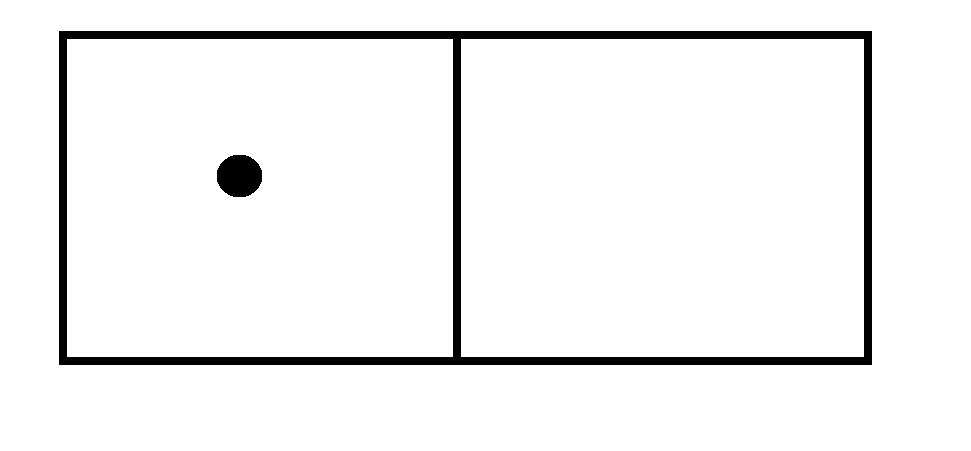
\includegraphics[width=0.5\textwidth]{ART_Kycia_Niemczynowicz/Demon2.png}
 \caption{In this case the particle is located in the left chamber of the box.}
 \label{Fig.Szilard_ParticleLocated}
\end{figure}
%%%%%%%%%%%

In the next step, the border between the chambers become movable. Energy is extracted when the gas is decompressed isothermally. This decompression is a reversible thermodynamic process and the work done by the particle is given by: 
\begin{equation}
 W=k_{B}T\int_{V/2}^{V}=k_{B}T \ln{2}.
\end{equation}
The situation is presented in Fig. \ref{Fig.Szilard_WorkExtraction}.
%%%%%%%%%%%
\begin{figure}
\centering
 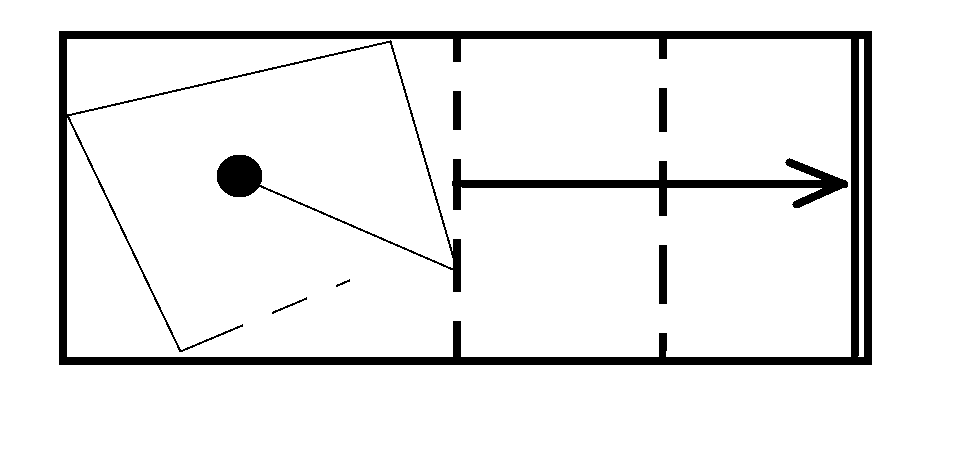
\includegraphics[width=0.5\textwidth]{ART_Kycia_Niemczynowicz/Demon3.png}
 \caption{Energy extraction in the isothermal expansion of a single particle of the ideal gas.}
 \label{Fig.Szilard_WorkExtraction}
\end{figure}
%%%%%%%%%%%

The final part of the cycle is the restart. The demon takes the border out of the box, moves it and then re-insert it again in the middle. We return here to the situation from Fig. \ref{Fig.Szilard_StateUnknown}. At this stage, information about the particle location is not needed, so the demon must delete it to return the whole system (box and demon) to the initial state for another round of the cycle. Therefore, we now have the same state as at the beginning of the previous turn.

This situation can be analyzed in terms of the second law of thermodynamics and entropy $S$. The second law of thermodynamics says that the change of total entropy (system and environment) must be non-decreasing.

In the case above, in the cycle, according to the conservation of energy (the first law of thermodynamics), the heat from the environment (the thermal bath of the particle) is extracted and used to make work $W$. Therefore, the deficiency of heat is $Q=W=k_{B}T\ln(2)$. Given that the balance is negative and the system is held at a constant temperature, the entropy change in the cycle is
\begin{equation}
 \Delta S = -\frac{Q}{T}=-k_{B}\ln(2) <0.
\end{equation}
This contradicts the second law (it must be $\Delta S \geq0$).

To solve this apparent contradiction,  \textcites{BennetDemon} has suggested that during the demon's erasure of the bit of information regarding particle location (say $0$--the particle in the left chamber, $1$--the particle in the right chamber) the heat of value $Q_{e}$ is expelled. This heat is no less than Landauer's bound (\ref{Eq.LandauersBound}), that is $Q_{e} \geq Q_{L}$. This assumption corrects the balance of entropy:
\begin{equation}
 \Delta S = \frac{Q_{e}}{T}-\frac{Q}{T} \geq k_{B}\ln(2) - k_{B}\ln(2) =0.
\end{equation}

Bennett's explanation solves the long-standing paradox by employing Landauer's idea. It is interesting to note that the paradox remained unresolved until the 1970s. Moreover, its resolution is based on the idea of information, computing, and memory developed in the twentieth century and therefore not known to the fathers of thermodynamics. The solution can almost be regarded as manifest in the works of \textcites{Szilard} if his experiment is interpreted as a model for computer memory. This reinterpretation of Szilard's results is presented in the next section, which provides a more in-depth insight into the connection between information and its implementation.

%%%%%%%%%%%%%%%%%%%%%%%
\section{Memory}
%%%%%%%%%%%%%%%%%%%%%%%
Szilard's \textit{gedanken experiment} presented in the previous section can be used to construct a thermodynamic model of computer memory. We consider here the simplest case; a more detailed presentation for general memory for multivalued logic is given in \parencite{KyciaNiemczynowicz}.
%\enlargethispage{.5\baselineskip}

The implementation of a single bit thermodynamic memory is presented in Fig. \ref{Fig.BinaryCell}.
%%%%%%%%%%%
\begin{figure}[ht]
\centering
 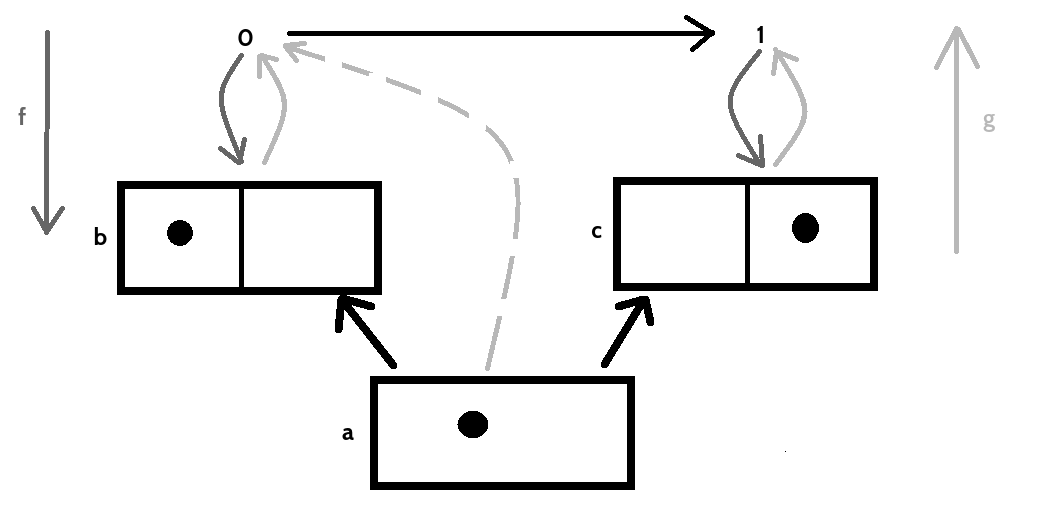
\includegraphics[width=0.7\textwidth]{ART_Kycia_Niemczynowicz/BinaryGalois-bw.png}
 \caption{Implementation of memory using the thermodynamic model of the reversed Szilard's model of Maxwell's demon. State $a$ is not associated with logical value: it is an undetermined internal state of the memory, which can be associated with $0$ at the logical level. State $b$ represents $0$, and state $c$ represents $1$. Maps $f$ and $g$, associating logical values with their physical implementation, are selected in such a way to preserve the order indicated by black lines representing transitions between states or ordering in Boolean algebra, that is, logic. This is a reminiscence of the Galois connection \parencite{SpivakSketches, CategoryGentleIntroduction, KyciaLandauer} that usually occurs where there is a system that contains an abstract level and its implementation.}
 \label{Fig.BinaryCell}
\end{figure}
%%%%%%%%%%%

State $a$ is an inner state of memory that does not represent any logical value. It is used to implement all logical operations (not necessarily those that swap $0$ and $1$). This assumption is consistent with the previous discussion of Szilard's model and its reverse. 

We can now proceed to a detailed description of the types of operations. At the level of logic, we have two types of operations on this memory:
\begin{itemize}
 \item {Reversible: operations that have inverses, i.e., those that are bijections, for instance, a NOT gate whose function is involutive: $0  \leftrightarrow 1$.}
 \item {Irreversible: operations that do not have inverse, for instance the assignment of some value that 'forgets' the previous value: ($0 \rightarrow 1$, $1 \rightarrow 1)$.}
\end{itemize}

At the level of thermodynamics, we have a similar convention. However, the definition is different:
\begin{itemize}
 \item {Reversible: realized by reversible thermodynamic processes, i.e. processes that can be reversed, or equivalently, the process that combined into a cycle with its inverse has vanishing entropy change $\Delta S =0$.}
 \item {Irreversible: realized by irreversible thermodynamic processes, i.e. if we perform this operation and then return (along any reversible process) to the initial state, then in the cycle $\Delta S >0$.}
\end{itemize}


As highlighted in \parencite{LandauerExplained}, the main idea behind Landauer's principle is the association of operations at the level of logic and their physical implementation in the form presented in Tab. \ref{Tab.LandauerConnection}; in our case, $A$ is the logical system and $B$ is its memory implementation.
%%%
\begin{table}
\centering
\begin{tabular}[!h]{|c|c|c|}
 \hline
 Possibilities &  \begin{tabular}{@{}c@{}}$B$ \\ reversible\end{tabular}  & \begin{tabular}{@{}c@{}}$B$ \\ irreversible\end{tabular} \\ \hline
 $A$ reversible & YES  & YES \\ \hline
 $A$ irreversible & NO & YES \\ \hline
\end{tabular}
\caption{Systems $A$ is implemented on $B$.} 
\label{Tab.LandauerConnection}
\end{table}
%%%


To understand this association, we provide some examples of logical operations and their physical implementations. 

To assign some initial value to memory state, let us start from state $a$ and perform isothermal compression to $b$. This initial preparation expels (stores) the heat $Q=k_{B}T\ln(2)$ to(in) the environment and sets the initial logical state to $0$.

Consider the reversible NOT operation. According to Tab. \ref{Tab.LandauerConnection}, this can be realized in two inequivalent thermodynamically ways at the physical level:
\begin{enumerate}
 \item {Reversible thermodynamic operation: isothermal expansion $b \rightarrow a$ and then isothermal compression $a \rightarrow c$. The composed operation is thermodynamically reversible and no heat is expelled to the environment or converted to work.}
 \item {Irreversible thermodynamic operation: we take the middle border out of the box, which generates free adiabatic decompression of the gas (particle) $b \rightarrow a$. Next, reversible isothermal compression $a \rightarrow c$ is made. When the first step is performed, we lose 'access' to the heat initially stored in $0$ state. This heat cannot be regained/reused and therefore must be treated as Landauer's heat.}
\end{enumerate}


Consider now the irreversible logical operation of setting $1$ starting from $0$. According to Tab. \ref{Tab.LandauerConnection}, this must be realized by an irreversible thermodynamic operation and hence it is the same as the operation from the second point above. Therefore, Landauer's heat is also expelled in this case.

This example is also proof that Landauer's principle is equivalent (at least for these examples) to the association from Tab. \ref{Tab.LandauerConnection} between operations on logical and thermodynamic states.


The presentation in this section was elementary, intending to be an introduction to the multivalued logic approach \parencites{KyciaNiemczynowicz, TritLandauer}, category theory formulation of this principle \parencites{KyciaLandauer, KyciaLandauer2}, mentioned briefly above, and its understanding in more fundamental level \parencite{LandauerExplained}. We also emphasize that the principle can be thoroughly understood only at the level of statistical physics \parencites{LandauerExplainedFull, Piechocinska}, and equilibrium thermodynamics used above is only its limiting case.

In the following conclusion section we briefly discuss the nature of information.


%%%%%%%%%%%%%%%
\section{Discussion}
%%%%%%%%%%%%%%%

The thermodynamic realization of a bit of information is a simple model that presents how Landauer's heat is generated for irreversible operations. In this model, energy is initially stored in the environment by setting some starting value ($0$ or $1$) in the memory. An irreversible operation then makes it impossible to reuse/regain this heat to perform work and thus extract energy from the memory to gain the initially 'invested' energy. In this interpretation, a bit labels the state of a system that contains energy that can be accessed and (re)used. Reversible operations are designed to extract this energy, whereas irreversible ones lose it. Therefore, according to the laws of thermodynamics, for irreversible operation, heat is expelled. 

Abstracting even more, the information is stored in some sort of energy configuration of the physical system. From the mathematical viewpoint, there is an abstract notion of information (bits, Boolean algebras), but ultimately information must be represented by certain physical states, allowing it to interact with the physical world. This storing process of information forms a connection between its abstract notion and the physical world.

This also has some practical consequences to philosophy. The 'sacrum' (abstraction) cannot be separated from 'profane' (realization). Abstract concepts (encoded as some form of information) must always be stored in some physical configuration of matter/energy. Information is a type of emergent concept or a new complexity built on top of physical constructs and our ability to manipulate energy and matter. This is a highly pragmatic approach. 

This perspective shows that information, although immaterial concept, exists in the Universe as its encoding/representation in physical content of matter and energy. Their properties can be abstracted, however, we always deal and interact with some of its representation. The connection between abstract notion and its multiple (physical) representations is also reflected in the Galois connection \parencite{CategoryGentleIntroduction}---a process of abstraction---which can be seen as a modern allegory of Plato's cave---a projection of mathematical (ideal) entity to the concrete realization (shadow on the cave wall).



%%%%%%%%%%%%%%%
\section{Conclusion}
%%%%%%%%%%%%%%%
We presented an overview of the basic facts from the thermodynamics of Maxwell's demon, its model by Szilard and the resolution of this paradox by Landauer. This motivated us to consider the correspondence between information and its physical representation. The aim was to introduce a broad audience to the basics of this subject and provide some references that can be used for more in-depth studies.


%%%%%%%%%%%%%%%%%%%%%%%%

\paragraph{Acknowledgments} We would like to thank anonymous Referees for useful comments and remarks that helped us improve the paper.

RK was supported by the GACR grant GA19-06357S, the grant 8J20DE004 of Ministry of Education, Youth and Sports of the CR, and Masaryk University grant MUNI/A/0885/2019. We would like to acknowledge COST CA18223 action for support.

 
 \end{artengenv2auth}



\begin{artengenv2auth}{Steve Awodey, Michael Heller}
	{The homunculus brain and categorical logic}
	{The homunculus brain and categorical logic}
	{The homunculus brain and categorical logic}
	{\textsuperscript{1}Departments of Philosophy and Mathematics, Carnegie Mellon University\\
		\textsuperscript{2}Copernicus Center for Interdisciplinary Studies, Jagiellonian University}
	{The interaction between syntax (formal language) and its semantics (meanings of language) is one which has been well studied in categorical logic. The results of this particular study are employed to understand how the brain is able to create meanings. To emphasize the toy character of the proposed model, we prefer to speak of the homunculus brain rather than the brain \textit{per se}. The homunculus brain consists of neurons, each of which is modeled by a category, and axons between neurons, which are modeled by functors between the corresponding neuron-categories. Each neuron (category) has its own program enabling its working, i.e. a theory of this neuron. In analogy to what is known from categorical logic, we postulate the existence of a pair of adjoint functors, called Lang and Syn, from a category, now called BRAIN, of categories, to a category, now called MIND, of theories. Our homunculus is a kind of ``mathematical robot'', the neuronal architecture of which is not important. Its only aim is to provide us with the opportunity to study how such a simple brain-like structure could ``create meanings'' and perform abstraction operations out of its purely syntactic program. The pair of adjoint functors Lang and Syn model the mutual dependencies between the syntactical structure of a given theory of MIND and the internal logic of its semantics given by a category of BRAIN. In this way, a formal language (syntax) and its meanings (semantics) are interwoven with each other in a manner corresponding to the adjointness of the functors Lang and Syn.  Higher cognitive functions of abstraction and realization of concepts are also modelled by a corresponding pair of adjoint functors.  The categories BRAIN and MIND interact with each other with their entire structures and, at the same time, these very structures are shaped by this interaction.}
	{categorical logic, syntax-semantics, mind-brain}
	{%
		{\flushright\subbold{Steve Awodey}\\\subsubsectit\small{Departments of Philosophy and Mathematics, Carnegie Mellon University}\par}%
		{\flushright\subbold{Michael Heller}\\\subsubsectit\small{Copernicus Center for Interdisciplinary Studies, Jagiellonian University}\par}%
	}
	
	



\section{Introduction: On the Computer Screen}
\lettrine[loversize=0.13,lines=2,lraise=-0.03,nindent=0em,findent=0.2pt]%
{W}{}e were preparing a paper for publication. A phase portrait was nicely displayed on the computer screen. The network of trajectories represented a class of solutions to the equation we were interested in. At some points, called critical points, certain trajectories crossed each other. These points were important for our analysis. Some of the diagrams we worked with appeared later as figures in our publication \parencite{GRG}. The figures had to be explained, so we decided to attach appropriate labels to some of the critical points. We attached the label ``stable saddle'' to one of them. No problem. Then we proceeded to attach the label ``unstable saddle'' to another one. But the label jumped up. We tried to fix it up, but it jumped down. Then we started laughing. After all, it is an unstable point!

Let us try to understand the situation. We were investigating an equation that (virtually) contains in itself its space of solutions (irrespectively of whether we explicitly know them or not). Through the suitable computer program and some ``electronic circuits'', which are activated by the program, this space of solutions is mapped into the phase portrait displayed on the computer screen. The diagram we see on the screen is certainly something more than just a picture. It does not simply show stable and unstable critical points; it also does what the abstract equation orders its solutions to do (labels jump up and down at instabilities).

Let us go a step forward. In fact, the phase portrait on the screen is a substitute of the world. For suppose that our equation ``describes'' (or better -- models) a mechanical system (e.g., a pendulum or oscillator).\footnote{The equations we considered in our publication referred to a cosmological situation.}  Then the unstable critical points of our equation correspond to physical situations in which the considered mechanical system behaves in an unstable way. We thus have, on the one hand, an equation (or a set of equations) or, more broadly, a mathematical theory and, on the other hand, a domain (or an aspect) of the physical world of which the considered mathematical theory is a model. Between the mathematical model and the domain (or aspect) of the physical world there is a mysterious correspondence -- a correspondence in the root-meaning of this word: both sides co-respond to each other. It is an active correspondence, and the activity goes both ways: it looks as if the domain of the world informed the theory about its own internal structure, and the theory answered by prescribing what the domain should do. And the domain does it. The equations prescribe what the world should do, and the world executes this. The equations and the world  are coupled with each other and act in unison.

And the screen on my computer? It is a part of the world. The program we have constructed reads the structure of the equations and executes what the equations tell it. And because of the coupling between the equations and the world, the computer does, in miniature, what does the world on its own scale. This is the reason why computers are so effective in our reading of the structure of the world.

There is another domain in which a formal structure reveals its effective power and produces real effects. Such processes occur in the brain. The formal structure in question consists of electric signals propagating along nerve fibres between neurons across synapses, and the world of meanings should be regarded as a product of this activity. The interaction seems to go both ways: the ``language of neurons'' (what happens in the brain) produces the meanings related to this language (in the mind), and the meanings somehow influence the architecture of neurons. 

It seems that in both these cases (mathematical laws and their effects in the real world, and the brain--mind interactions) we meet two instances of the same working of logic where syntax (a formal structure), by effectively interacting with its semantics, produces real effects. This kind of interaction, although kept strictly on the level of logic (i.e. with no reference to processes in the real world), is well known in the categorical logic. In the present paper, we attempt to employ these achievements of categorical logic to try to understand the brain--mind interaction. 

The traditional terminology of brain and mind (irrespective of current trends in cognitive sciences to get rid of their conceptual load) seems especially well adapted to the present context in which general ideas are more important than structural details. Moreover,  to avoid too hasty associations with the human brain and to emphasize the toy character of the proposed model, we prefer to speak of the ``homunculus brain'' rather than just of brain.

The action of our argument develops along the following lines. Section 2 is a reminder on formal language, its syntax and semantics. Sections 3 and 4 briefly review those parts of categorical logic that refer to these concepts. Every category, call it $C$, has its internal logic, and if this logic is sufficiently rich, the category provides semantics for a certain formal theory $T$. Moreover, there exists a pair of adjoint functors, called Lang and Syn, from a category, called CATEGORIES, of categories belonging to a certain class  (for instance, coherent categories) to a category, called THEORIES, of theories and \textit{vice versa}, which describe mutual dependencies between the syntactical structure of $T$ and the internal logic of its semantics given by $C$. This is described in section 3. In this way, syntax and semantics are interwoven with each other in a manner corresponding to the adjointness of the functors Lang and Syn. This is explored in section 4.  In section 5, we consider a deep categorical duality between the syntactic category of a theory and its individual models and suggest a functional interpretation in terms of abstraction and realization of concepts, in anticipation of the cognitive interpretation to be introduced next.
In section 6, the category CATEGORIES becomes the category BRAIN. It constitutes a simple model of a homunculus' brain. Objects of this category are categories (belonging to a certain class); every such category models a neuron. Morphisms of this category model signals propagating along nerve fibres between neurons. The category THEORIES becomes the category MIND. Its objects are ``theories of neurons''; more precisely, if $C \in $ BRAIN, then its ``theory'' is Lang$(C)$ in MIND. Morphisms of this category are functors between the corresponding syntactic theories; more precisely, if $T_1, T_2 \in $ MIND, then the morphism between them is $\mathrm{Syn}(T_1) \to \mathrm{Syn}(T_2)$. The pair of adjoint functors Lang and Syn model the interaction between the syntax of ``theories'' and their semantics, i.e. the network of neurons. The categories BRAIN and MIND are indeed somehow related to what their names refer to, at least as far as homunculus' brain and mind are concerned.

Following the seminal paper of %W.S.~McCulloch and W. Pitts 
\citeauthor{McCulloch}, published as early as in \cite*{McCulloch}, which proposed using classical logic to model neural processes in the brain, there have been so many papers developing and modifying (with various logical systems) this idea, that to quote even a sample of them would be immaterial \parencite[for a relatively recent state of art see a short review][]{Koch}. A.~\citeauthor{Ehresmann} claims that it was R.~\citeauthor{Rosen} who was the first to employ category theory to model biological systems. A series of works followed (a non-representative sample: \parencites{Gomez}{Healy}{Mizraji}{Naotsugu}) proposing  the use of various parts of category theory to model different aspects of the brain activity. In particular, adjoint functors were suggested to model ``a range of universal-selectionist mechanisms'' \parencite{Ellerman}. However, we have not been able to find anything similar to modeling the interaction between brain's language and its meaning anywhere.

\section{Syntax and Semantics}
In linguistics, syntax and semantics are regarded as parts of semiotics, the study of signs. Syntax studies relations between signs, and semantics relations between signs and what the signs refer to.\footnote{Sometimes one also distinguishes pragmatics which studies relations between signs and their users.} Syntactic properties are attributed to linguistic expressions entirely with respect to their shape (or form). Semantics, on the other hand, endows them with meaning by referring signs to what they signify. Logic adapts these ideas to its own needs. Since it is a formal science, the signs it considers should be elements of a formal language, and they cannot refer to anything external. Halvorson puts it, ``But a formal language is really not a language at all, since nobody reads or writes in a formal language. Indeed, one of the primary features of these so-called formal languages is that the symbols don't have any meaning'' \parencite{Halvorson2016}. This is why the meaning should be ``artificially'' constructed for them. The idea of how this should be done can best be seen in Tarski's prototype of this procedure \parencite{Tarski}. If a sentence $s$, the truth of which we want to define, belongs to a language $L$ then the definition of $s$ should be formulated in a metalanguage $M$ with respect to the language $L$. And the metalanguage $M$ should contain a copy of $s$ so that anything one can say with the help of $s$ in $L$, can also be said in $M$. The definition of ``True'' should be of the form

\begin{center}
For all $x$, True$(x)$ if and only if $\varphi (x)$
\end{center}
with the condition that ``True'' does not occur in $\varphi $. Here $x$ stands for the copy of the sentence $s$ in the metalanguage $L$, and $\varphi(x)$ describes, also in $M$, the state of affairs of which the sentence $s$ in $L$ reports \parencites[for more details see][]{Stanford}{Gila}. A metalinguistic copy of $s$ could also be expressed as ``$s$'' (taken in quotes). In Tarski's own example:
\begin{center}
``It snows'' is true iff it snows.
\end{center}
For pedagogical reasons, this example is taken from colloquial language, but strictly speaking Tarski's definition refers to formal languages. The formal language $L$ has its own syntax (since it is a formal language), but is lacking its semantic reference. As we have seen, such a reference had to be constructed for it with the help of the metalanguage $M$.

Now, the idea is to improve the situation by looking for such a conceptual context in which a semantics for a given theory would arise in a more natural (or even spontaneous) way.

\section{Categorical Semantics}
To do so we must first define precisely what we mean by language. Since the definition must be precise, let us choose as an example the language of mathematics based on standard first order logic (which is enough for most of the usual mathematics). Many other languages may be formalized in a similar way. In such a language we distinguish:
\begin{itemize}
\item constants: $0, 1, 2,\ldots , a, b, c,\ldots ,$ and variables: $x, y, z,\dots $, which can be combined by primitive operations to give
\item terms, for example: $x+y, \, x^3, \ldots $ which, in turn, can be combined, with the help of primitive relations, such as $=, <, \leq, \dots $, to produce
\item formulae, for example: $x+y = z, \, x \leq y,\ldots $ which, in turn can be combined, with the help of the usual logical connectives and quantifiers, into
\item more complicated formulae.
\end{itemize}

To make the language more flexible and more adapted for concrete applications, we diversify its expressions into various types (called also sorts). In mathematics, we might use different letters for natural and real numbers, or different symbols for vectors an scalars. We say that, in both cases, we are using a two-typed language.  There may be languages with as many types as is needed.

What we need is not so much a language, but rather a theory. In mathematical logic theory is almost the same as language; it is a formal language aimed at axiomatizing a certain class of sentences. The concept of theory, as it is functioning in modern physics can, in principle, be regarded as the special case of the logical concept of theory, although in scientific practice theories are rarely formulated with the full logical rigor.  

Let then $T$ be a theory expressed in a multi-type language.  Such a theory is defined as consisting of the following data:
\begin{enumerate}
\item
A set of types $\{X_1, X_2, \ldots, X, Y, \ldots\; \}$.
\item
A set of variables $\{x, y, z, \ldots ,\, x_1, x_2, x_3, \ldots \}$ with a type assigned to each variable.
\item
A set of function symbols with a type assigned to each domain and codomain of every function symbol; for instance, to the term $x_1+x_2$, with the variable $x_1$ of type $X_1$ and the variable $x_2$ of type $X_2$, there corresponds the function symbol $f: X_1 \times X_2 \to Y$, and the term $f(x_1,x_2) = x_1+x_2$ is of type $Y$.
\item
A set of relation symbols with a type assigned to each argument of every relation symbol; for instance, to the formula $x+y=z$, with the variable $x$ of type $X_1$, the variable $y$ of type $X_2$ and the variable $z$ of type $X_3$, there corresponds the relation symbol $R \subseteq X_1 \times X_2 \times X_3$, and $R(x,y,z)$ is an atomic formula.
\item
A set of logical symbols.
\item
A set of axioms for a given theory built up from terms and relation symbols with the help of logical connectives and quantifiers, respecting types of all terms.
\end{enumerate}
This is, in fact, a purely syntactic definition of theory \parencites[for details  see][pp.344--348]{Borc}[][pp.527--530]{MacLaneMoerdijk}. Now, we want to create a semantics, i.e. a model, for a theory $T$. This is done by constructing a category $C_T$ which will serve us as such a model. The construction is almost obvious:
\begin{enumerate}
\item
each type of $T$ is an object of $C_T$, 
\item
for each function symbol $f$ in $T$ with types $A$ and $B$ as its domain and codomain, correspondingly, $f$ is a morphism from the object $A$ to the object $B$ in $C_T$,\footnote{Since $f$ is now regarded as being in $C_T$ rather than in $T$, it should formally be denoted by a different symbol such as $[f]$, but we omit such formalities for present purposes.}
\item
variables are identity morphisms in $C_T$,
\item
for each relation symbol $R$ in $T$, its counterpart in $C_T$  is a subobject in $C_T$. Suppose $\phi $ is a subobject of an object $A$ in $C_T$ then, by analogy with the usual theory of sets, $\phi $ can be thought of as a collection of all things of type $A$ that verify $\phi $.
\end{enumerate}
This definition must be supplemented with all of the (first order) logic which is used to express axioms in $T$ \parencite[for details see][]{nLab2}. Roughly speaking, since formulae correspond to subobjects, and all subobjects of a given object are partially ordered by inclusions (they form a poset), the axioms can be expressed in terms of the order relation on the subobject poset in the category $C_T$.
The category, defined in this way, is appropriately called the categorical semantics for a theory $T$.

We have thus created (almost automatically!) a domain (the category $C_T$) the theory $T$ refers to. The internal architecture of the category $C_T$ exactly matches the logic involved in the theory $T$. 

Let us also mention that, \textit{vice versa}, having a (sufficiently rich) category $C'$, we can construct the formal theory $T'$ the logic of which matches the internal architecture of the category $C'$. This can be done by reading the above definition of the categorical semantics ``backwards'', i.e. we regard objects of $C'$ as types of $T'$, identity morphisms of $C'$ as variables in $T'$, etc. The theory $T'$, reconstructed in this way from the category $C'$, is called internal logic of $C$. This entire process can be regarded as a functor, called Lang, from a category of categories, call it CATEGORIES, to a category of theories, call it THEORIES,
\begin{center}
Lang: CATEGORIES $\to $ THEORIES.
\end{center}
For the time being this definition remains informal since neither CATEGORIES nor THEORIES have been properly defined, but it will be done below. 

Let us start with a formal theory $T$. We now want to organize it into a category Syn$(T)$, called the syntactic category of $T$. It is done in the following way.

Let $\Gamma $ be a collection of type assertions, i.e. a collection of rules assigning a type to each term of a given theory, and $\Phi $ a collection of all well-defined formulae of $T$. The pair $(\Gamma , \Phi )$ is called a context. It is a formalization of what in ordinary language one means by this term.

If $T$ is a type theory, its syntactic category, Syn($T$), is defined as follows. Its objects are contexts $(\Gamma , \Phi )$ and its morphisms $(\Gamma , \Phi ) \to (\Delta , \Psi )$ are interpretations (or substitutions) of variables. The latter means that for each type, prescribed by $\Delta $, we must construct an expression of this type out of data contained in $\Gamma $. In general, this is done by substituting terms from $\Gamma $ for variables in $\Delta $. We must also present, for each assumption required by $\Delta $ (if there are any), a proof of this assumption from the assumptions contained in $\Gamma $ \parencite[for details see][]{Fu,nLabSyn}. 

The category Syn($T$), constructed in this way, is also called a category of contexts \parencite[for details see][]{Fu,nLabSubs}). 

Since from a theory $T$ we have constructed the category Syn($T$), we can have a  functor,
\begin{center}
Syn: THEORIES $\to$ CATEGORIES
\end{center}
provided we define the categories THEORIES and CATEGORIES. We do this in the next section.

\section{Syntax--Semantics Interaction}
Let us start with objects for both of these categories. It is obvious that they will be categories and theories, respectively. To have  workable categories, one must restrict the class of theories as candidates of being objects in THEORIES (and analogously for CATEGORIES). The criterion one follows is the kind of logic that underlines a given theory. It could be what logicians call: finite product logic, regular logic, coherent logic, geometric logic, etc.\footnote{As it could be expected, the internal logic of the corresponding semantic category will be of the corresponding kind, i.e. finite product logic, regular logic, etc. \parencite{nLab2}.} For our further analysis it is irrelevant which one will be chosen. However, for the sake of concreteness we may think about coherent logic. Roughly speaking, this is a fragment of the first order logic which uses only the connectives $\wedge $ and $\vee $, and the existential quantifier. Large parts of mathematics can be formalised with the help of this logic. To this logic there correspond coherent theories and coherent categories. They will constitute objects of THEORIES and CATEGORIES, respectively.
Morphisms for CATEGORIES are obviously functors between corresponding categories; for instance coherent functors for coherent categories \parencite{nLabCoherent}.  Let now $T_1$ and $T_2$ be objects in THEORIES. A morphism $T_1 \to T_2$ is a functor between their corresponding syntactic theories $\mathrm{Syn}(T_1) \to \mathrm{Syn}(T_2)$. Roughly speaking, this means that it is possible to express (to interpret) $T_1$ in terms of $T_2$ \parencite[for details and discussion see][]{Halvorson2017}.\footnote{Strictly speaking, CATEGORIES is a 2-category (since its objects are categories and morphisms are functors), and THEORIES is a 2-category, in this case, called also a doctrine \parencite{nLabDoctrine}.}

As a side remark let us notice that by studying the category THEORIES, we could learn ``how individual theories sit within it, and how theories are related to each other'' \parencite[p.413]{Halvorson2017}. This is nicely consonant with a newer trend in the philosophy of science to investigate the so-called inter-theory relations \parencite{Batterman,Rosaler}.

A truly remarkable fact is that the functors Lang and Syn constitute a pair of adjoint functors. Let us explain precisely what this means.

Let us consider any pair of objects: $\mathcal{C}$ of CATEGORIES and $T$ of THEORIES. Adjoint functors serve to compare them. However, they cannot be compared directly since they live in different categories. Adjoint functors serve to move each of them to the correct category so as to enable the comparison. Let us follow this process step by step \parencite[pp.148-153]{Simmons}.

Let us first consider the object $T$ which lives in THEORIES. We want to compare it with the object $\mathcal{C}$ which lives in CATEGORIES. We thus move $\mathcal{C}$ to THEORIES with the help of the functor Lang to obtain the object Lang($\mathcal{C}$). We now make the comparison with the help of a suitable morphism,
$$
f: \mathrm{Lang}(\mathcal{C}) \to T
$$
in THEORIES. We do the same starting with $\mathcal{C}$ in CATEGORIES and $T$ in THEORIES, and compare $\mathcal{C}$ with Syn$(T)$, 
$$
g: \mathcal{C} \to \mathrm{Syn}(T)
$$
in CATEGORIES. To complete the definition of adjunction we demand that morphisms $f$ and $g$ should constitute a pair of bijections which is natural both in $\mathcal{C}$ and $T$ (see below).

The above definition can be put into a concise form
\begin{equation}
\label{hom1}
\mathrm{THEORIES}(\mathrm{Lang}(\CC ), T) \cong {\mathrm{CATEGORIES}}(\CC , \mathrm{Syn}(T)),
\end{equation}
expressing an isomorphism between the right and left hand sides of this formula that is natural in $\mathcal{C}$ and $T$. The latter condition says that when \CC \ varies in CATEGORIES and $T$ varies in THEORIES, the isomorphism between morphisms $\mathrm{Lang}(\CC ) \to T$ in THEORIES and $\CC \to \mathrm{Syn}(T)$ in CATEGORIES vary in a way that is compatible with the composition of morphisms in CATEGORIES and THEORIES, correspondingly, and with the actions of Lang and Syn on both these categories \parencites[see][]{AF}[][pp.50-51]{Leinster}.\footnote{For a full definition of adjoint functors see any textbook on category theory.}

We should notice that in the above definition, in fact, we not only compare objects of two different categories, but rather categories themselves (objects $\mathcal{C}$ and $T$ are any pair of objects). Moreover, comparing two categories we are not so much interested in their objects, but rather in morphisms between objects. This is clear from the fact that at the end, we have identified those morphisms of two categories that are pairwise naturally isomorphic among themselves.

As we can see, categorical logic does not simply create a semantics for a given language, but shows that dependencies between them go both ways: in a sense, syntax and semantics create each other. More precisely, they condition each other through the adjointness relation.

%
% SA additions begin here
%
\section{Realization and Abstraction}

There is another aspect of categorical logic that we shall make use of, and it may be seen as a mathematical description of the processes of abstraction and realization of concepts. The category $\mathrm{Syn}(T)$ representing a theory $T$ may be regarded as presenting a general \emph{concept}, of which the theory $T$ is a particular syntactic description.  For example, there is a theory $T_{Group}$ consisting of 
a single basic type $X$, and function symbols $* : X\times X\to X$ and $(-)^{-1} : X \to X$ and a constant $u : X$, together with the usual equations for groups as its axioms:
\begin{align*}
x*(y*z) &= (x*y)*z\\
x*u &= x\\
u*x &= x\\
x*x^{-1} &= u\\
x^{-1}*x &=u
\end{align*}
The syntactic category $\mathrm{Syn}(T_{Group})$ then represents the general concept of a group.  This concept can also be represented by another theory $T_{Group}'$ with a different choice of basic equations, or even a different choice of operations,\footnote{For example there is an axiomatization of groups using a single ternary operation in place of the two operations $x*y$ and $x^{-1}$.} as long as the resulting categories $\mathrm{Syn}(T_{Group})$  and $\mathrm{Syn}(T_{Group}')$ are equivalent.

A general concept may have many individual \emph{instances}; an instance of the concept of a group is, of course, just a particular group: a set $G$ of elements, equipped with functions interpreting the operations of multiplication and inverse, and satisfying the group equations.  A logician would call such an instance a \emph{model of the theory of groups}, but we shall avoid this over-worked term and refer to it instead as a \emph{realization} of the theory of groups.  A realization of a theory $T$ in any category $\CC$ is essentially the same thing as a functor $\mathrm{Syn}(T) \to \CC$ that preserves the relevant structure of the theory -- in the case of groups, the finite products $X\times X$.  (This is in fact the defining universal property of the syntactic category $\mathrm{Syn}(T)$.)  The realizations in the category SET, consisting of all sets and functions, are thus exactly what we called the \emph{instances} of the general concept of a group, namely groups.  

The standard category $\mathrm{GROUP}$ of all groups and their homomorphisms, as usually defined in abstract algebra, is then essentially the same as the category of all such instances, that is, the category $\mathrm{REAL}(\mathrm{Syn}(T_{Group}), \mathrm{SET})$ of all $\mathrm{SET}$ realizations, i.e.\ (structure-preserving) functors, where the morphisms are just natural transformations of such functors (that these correspond exactly to group homomorphisms is not trivial).  In this way, for any general concept $\mathrm{Syn}(T)$ corresponding to a theory $T$ we can define the category of its $\mathrm{SET}$ realizations, 
\[
\mathrm{REAL}(T) =_{df} \mathrm{REAL}(\mathrm{Syn}(T), \mathrm{SET}),
\]
which may be viewed as the category of instances of the concept $\mathrm{Syn}(T)$.

Now an amazing and mathematically deep fact emerges, which can only be seen using the tools of categorical logic: from the category  $\mathrm{REAL}(T) $ of all instances of the concept presented by $T$, one can actually recover the general concept $\mathrm{Syn}(T)$.  Indeed, for any structured category $\mathcal{R}$ of the same kind as $\mathrm{REAL}(T)$ (we will say a bit more about the condition ``of the same kind'' below), one can consider all of the \emph{continuous} functors $f : \mathcal{R} \to \mathrm{SET}$; these may be regarded as ``images'' or ``abstractions'' of the (generalized) realizations in $\mathcal{R}$.  The category of all such abstractions $\mathrm{ABSTRACT}(\mathcal{R}, \mathrm{SET})$ (again, with natural transformations as morphisms) may be called the \emph{abstract} of $\mathcal{R}$, and written simply 
$$
\mathrm{ABSTRACT}(\mathcal{R}) =_{df}  \mathrm{ABSTRACT}(\mathcal{R}, \mathrm{SET}).
$$
A similar construction that the reader may know is the ring $\mathcal{C}(X) = \mathcal{C}(X, \mathbb{R})$ of continuous, real-valued functions on a space $X$. The noteworthy fact that we mentioned above is this: if for $\mathcal{R}$ we take a category $\mathrm{REAL}(T) $ of realizations of a theory $T$, then the abstract of $\mathrm{REAL}(T) $, consisting of all ``abstractions'' $\mathrm{REAL}(T) \to \mathrm{SET}$, will be the associated concept $\mathrm{Syn}(T)$.\footnote{Under suitable assumptions, and up to the relevant notion of equivalence, of course; see \parencite{Awodey2019} for the general theory.}   Thus \emph{the abstraction of the realizations of a concept is the concept itself}.  We can even summarize this briefly by saying that \emph{All concepts are abstract}, since every concept is the abstraction of its realizations.  More generally, for any suitable category $\mathcal{R}$, the category $\mathrm{ABSTRACT}(\mathcal{R})$ of all continuous functors $f : \mathcal{R} \to \mathrm{SET}$ (the ``abstractions'' of $\mathcal{R}$) is a general concept, of which $\mathcal{R}$ is either the category of realizations, or an approximation thereof.  

The general correspondence is given by a (contravariant!) adjunction between the \emph{functors} of Realization and Abstraction which relate these operations; schematically,
\[
\xymatrix{
\mathrm{CONCEPTS}  \ar@/^4ex/ [r]^{\mathrm{Realization}} & \ar@/^4ex/ [l]^{\mathrm{Abstraction}} \mathrm{INSTANCES}^{op}
}
\]

Here $\mathrm{CONCEPTS}$ is the category consisting of all ``conceptual'' categories $\mathrm{Syn}(T)$ and their (relative) ``realizations'', i.e.\ functors  $\mathrm{Syn}(T) \to \mathrm{Syn}(T')$, and the functor of Realization is defined by taking realizations in $\mathrm{SET}$,
\begin{align*}
\mathrm{Realization}(\mathrm{Syn}(T)) = \mathrm{REAL}(\mathrm{Syn}(T), \mathrm{SET}),
\end{align*}
which we also called the category of ``instances'' of the concept. 

And $\mathrm{INSTANCES}$ is the category consisting of all (generalizaed) categories of instances $\mathcal{R}$ (such as the categories $\mathrm{GROUP}$, $\mathrm{RING}$, etc.) with their ``continuous'' functors  $\mathcal{R} \to \mathcal{R'}$, and the functor of Abstraction is defined by taking continuous functors into $\mathrm{SET}$, 
\begin{align*}
\mathrm{Abstraction}(\mathcal{R}) = \mathrm{ABSTRACT}(\mathcal{R}, \mathrm{SET}),
\end{align*}
which we called ``abstractions'' of the category $\mathcal{R}$. 

Let us consider a simple example!  Propositional logic consists of basic propositional variables $x, y, z, \dots$ and constants $\top, \bot$, which can be made into formulae using the usual propositional connectives $\neg z\,, x \wedge y\,, x\vee y\,, x\Rightarrow z$, and which are assumed to satisfy the usual logical laws, such as $x \wedge (y\vee z) = (x \wedge y)\vee (x \wedge z)$\,, $\neg\neg x = x$, etc.  A \emph{theory} $T$ in this simplified case is just a set of propositional letters $V = \{p_1, p_2, \dots, p_n\}$ (regarded as $0$-ary relation symbols), and a list of propositional formulae $A = \{\alpha_1, \alpha_2, \dots, \alpha_m\}$ built up from these letters, as the axioms of the theory.  There are no types, typed variables, or function symbols (or rather, there is a single, implicit type $1$), and the logical symbols are just the propositional connectives.

The \emph{syntactic category} $\mathrm{Syn}(T)$, representing the ``concept'',  is then the Boolean algebra $F(V)/A$ obtained as the free Boolean algebra $F(V)$ on the variables $V$ as generators, quotiented by the filter generated by the axioms $A$.  This ``concept'' associated to the propositional theory $T = (V,A)$ is independent of the particular syntactic presentation $(V,A)$.  A \emph{realization} of $T$ is then a boolean homomorphism $F(V)/A \to 2$, where $2 = \{0,1\}$ is the Boolean algebra of truth values.  Thus such a realization is just a truth-value assignment to the variables in $V$, in such a way that the ``conditions'' in $A$ are all satisfied, i.e.\ the elements $a\in A$ are all taken to the value ``true'' (in other words, a ``model'' of the propositional theory $T$).  For instance, if the theory $T$ is $V= \{x, y\}$ and $A = \{x\vee y, \neg(x\wedge y)\}$, then a realization would be an assignment of $x$ to an actual sentence $p$, and $y$ to one $q$, such that only one of $p$ and $q$ is true (or more formally, a direct assignement of such truth values, by-passing the actual sentences).  Under our description above, such a realization is an instance of the general concept $F(V)/A$.

Now, such realizations are exactly the points of the \emph{Stone space} $\mathrm{Stone}(F(V)/A)$, the topological space associated to the Boolean algebra $F(V)/A$ under the celebrated Stone duality theorem \parencite{Johnstone} -- which is in fact the ``propositional logic'' case of the categorical logical duality that we are considering here.  Formally, the points of $\mathrm{Stone}(F(V)/A)$ are prime filters in $F(V)/A$, and the topology has basic open sets determined by the elements of $F(V)/A$.  The Boolean algebra $F(V)/A$ can be recovered from this space $\mathrm{Stone}(F(V)/A)$ as the algebra of continuous functions $\mathrm{Stone}(F(V)/A)\to \mathsf{2}$ into the discrete space $\mathsf{2}$, with the pointwise Boolean operations.  These \emph{abstractions} of $\mathrm{Stone}(F(V)/A)$ form a Boolean algebra $\mathrm{Bool}(\mathrm{Stone}(F(V)/A))$ which, by Stone duality, is isomorphic to $F(V)/A$,
\[
\mathrm{Bool}(\mathrm{Stone}(F(V)/A))\ \cong\ F(V)/A\,.
\]  
Indeed, for any (not necessarily Stone) space $X$, we can form the Boolean algebra $\mathrm{Bool}(X)$ of continuous functions $X \to \mathsf{2}$, and the original space $X$ will then map canonically to $\mathrm{Stone}(\mathrm{Bool}(X))$, giving the ``best approximation'' of $X$ by a Stone space.

In the general case, in categorical logic we consider many other fragments of logic --- propositional, equational, coherent, first-order --- and for each such subsystem there is an associated Realization--Abstraction adjunction between theories, and the concepts they represent, on the one hand, and their realizations by instances of these concepts, on the other.  The propositional theories just considered give rise to Stone duality \parencite{Johnstone}; equational theories (like groups) give rise to Lawvere duality \parencite{ALR}; coherent and first-order logic are treated by analogous duality theories developed by Makkai and others \parencites{Makkai}{AF}.  In each diffferent case, the associated notion of structured category, structure-preserving functor, continuous functor, etc., is suitably adapted to the respective situation.  Many of these logical dualities are discussed from the standpoint of categorical logic in the paper \parencite{Awodey2019}.



\section{Categories BRAIN and MIND}
So far everything that has been said has merely been a reminder of standard and well-known things. From now on, everything will be hypothetical and highly simplified. The bold and maximally simplified hypothesis is that neurons in the brain can be modeled as categories, the internal logic of which is sufficiently complex (yet manageable). Of course, our inspiring motive is the human brain, and in constructing our model we shall try to imitate what is going in it; however, being conscious of our simplified and highly idealized assumptions, we prefer to speak about a homunculus brain. Our homunculus is a kind of ``mathematical robot'', the aim of which is to provide us with the opportunity to study how such a simple brain-like structure could ``create meanings'' out of its purely syntactic program. Our other drastically simplifying assumption consists in systematically ignoring all of the brain's functions and processes that are not directly related to the proposed syntax--semantics relationship.

As it is well-known, neurons communicate through signals transmitted via: presynaptic (source) neuron -- axon --  synapse -- dendrite -- postsynaptic (target) neuron, and this \textit{via} is unidirectional. In our homunculus model, these transmission processes will be regarded as functors between categories (neurons). 

Let us consider the category CATEGORIES, which we now aptly call BRAIN. Its objects are categories modeling neurons, and morphisms are functors between these categories.

We thus assume that each neuron in the homunculus brain is represented by a category (belonging to a certain class of categories; in the following we shall simply say that a neuron is a category). At the moment, we are not interested which biological mechanisms implement this assumption. Everything that counts in this model is the assumption that neurons consist of collections of objects and morphisms satisfying conditions from the category definition. We should have in mind that these simple conditions might lead to highly complicated structures.

Morphisms (arrows) in the category CATEGORIES are functors between object-categories, that is to say axons through which neurons communicate with each other. The crucial thing is that they must satisfy the usual conditions for morphisms: composition of morphisms, its associativity, the existence of identity morphisms. With the latter there is no problem: no output from a neuron counts as its identity morphism. To check whether two other conditions are verified in the human brain would require going deeper into the neural structure of our brain. In the case of the homunculus brain, this is not necessary. Since the homunculus is of our construction, we simply assume that synapses in its brain well-compose and do so in the associative way.

The next step seems obvious. Each neuron (modeled as a category $C \in $ BRAIN) has its own program enabling its working, i.e. an internal logic underlying this program. We thus can define a counterpart of Lang$(C)$ which is a ``theory'' of this neuron. It is reasonable to claim that it is an object of the category THEORIES which we now call MIND, and the functor Lang: BRAIN $\to $ MIND is defined in analogy to that between CATEGORIES and THEORIES.

What about the morphisms between such objects? We proceed in strict analogy with what has been done in THEORIES. Let now $T_1$ and $T_2$ be objects in MIND, a morphism between them, $T_1, \to T_2$, is a functor between their corresponding syntactic theories, i.e. $\mathrm{Syn}(T_1) \to \mathrm{Syn}(T_2)$, where the functor Syn: MIND $\to $ BRAIN is defined in analogy to that between THEORIES and CATEGORIES.

The analogy is only apparently straightforward. In fact, it is based on a huge extrapolation, and as such highly hypothetical, but it is worth exploring it since the problem at stake deserves even a higher risk. By pursuing this analogy we could claim that also in this case the functors Lang and Syn are adjoint functors. If so, we have a very interesting conjunction between brain and mind; it is interesting even if brain and mind are modeled by such a naive construction. 

Neurons, their interactions and programs underlying their working  are, in contrast with abstract categories like CATEGORIES and THEORIES, real things, at least in the homunculus world, and we are entitled to suppose that the functors Lang and Syn between Brain and Mind really do what they formally signify (like our phase portrait on the computer screen really did what the program told it to do). 

Roughly speaking the functor Lang provides a collection of theories (mind) for a collection of neurons (brain), and the functor Syn transfers the syntax of these theories to the network of neurons. The action of these two functors is adjoint; consequently it determines a strict interaction between BRAIN and MIND. Let $C$ be any object (a neuron) in BRAIN and $T$ any object (the theory of this neuron) in MIND, then equation (\ref{hom1}) assumes the form
\begin{equation}
\label{hom2}
\mathrm{MIND}(\mathrm{Lang}(\CC ), T) \cong {\mathrm{BRAIN}}(\CC , \mathrm{Syn}(T)).
 \end{equation}
The natural isomorphism $\cong $ appearing in this equation is crucial. It states that when we go from neuron to neuron as objects in BRAIN, and their corresponding theories vary in THEORIES, then the isomorphism between morphisms $\mathrm{Lang}(\CC ) \to T$ in MIND and $\CC \to \mathrm{Syn}(T)$ in BRAIN varies in a way that is compatible with the composition of morphisms in BRAIN and MIND, correspondingly, and with the actions of the functors Lang and Syn \parencites[see][]{AF}[][]{Leinster}.\footnote{For a full discussion of the role of the naturality condition in the definition of adjoint functors see any textbook on category theory.} 
%
% begin insertion by SA
Finally, the ``higher'' cognitive functions of abstraction and realization of concepts are modelled by a corresponding adjunction between the associated functors $\mathrm{Abstraction}$ and $\mathrm{Realization}$ relating these categories BRAIN and MIND. 
% end insertion by SA
%
We could summarise the situation by saying that the categories BRAIN and MIND interact with each other with their entire structures and, at the same time, these very structures are shaped by this interaction.

\section{A Comment}
The interactions between syntax and semantics are omnipresent both in our everyday conversations and in various forms of practicing science. The world around us is full of meanings and our attempts to decipher them. Science could be regarded as a machine to produce signs, through experimentation and critical reasoning, and  extracting from combinations of them information about the structure of the world. Logicians put a lot of effort to make the syntax--semantics interaction precise. As we have seen in section 2, despite the fact that formal languages are lacking any external references, it was possible to create semantical references for them  by cleverly exploiting the relation between language and its metalanguage. In categorical logic the situation has improved. Any formal theory $T$ generates via the functor Syn the category $\mathrm{Syn}(C)=C_T$ of which it is a theory, i.e. $C_T$ provides a ``natural'' semantics for $T$. And \textit{vice versa}, any (sufficiently rich) category $C'$, via the functor Lang, generates its own theory Lang$(C')=T'_{C'}$ which constitutes the internal logic of $C'$. It is interesting to notice that  $T_{C_T}$ does not coincide with $T$, they are only Morita equivalent. Here, we shall not go into technical details; it is enough to say that two Morita equivalent theories could be regarded as two interpretations of the same theory \parencite{Halvorson2016}.

The fact that $T_{C_T}$ does not coincide with $T$ is a consequence of the fact that the functors Lan and Syn are not mutually inverse functors but constitute a pair of adjoint functors. This in turn implies that in categorical logic the interaction between syntax and semantics is skillfully complex, with creative influences coming both ways.

All the above discussed properties of the syntax--semantics interaction can be presumed to be preserved if applied to the categories BRAIN and MIND. There is only one big difference: now ``neurons and their theories'' are real things (although in a highly idealised, toy version in the homunculus world). Nevertheless, the situation is not so different from the one which we can observe in many empirical sciences, in which some abstract mathematical structures model some real processes (always more or less idealised). We should not be surprised that the method of mathematical modeling  works when applied to our cognitive processes, but rather that mathematical structures not only describe the real world (whether it is our brain or the world of physics), but that they are also effectively acting in it (like in the little arrow on the computer screen). 
 
 
 \end{artengenv2auth}







%\sekcja{Z prac Komisji Filozofii Nauk PAU}{Proceedings of the PAU Commission\\\ on the Philosophy of Science}
%
%\input{ART_Kawalec/Kawalec-PU.tex}
%
%\input{ART_Czarnik/Czarnik-PU.tex}
%
%\input{ART_Szybka/Szybka-PU.tex}



%\addtocontents{toc}{\protect\pagebreak}



\sekcja{Recenzje}{Book reviews}

\begin{recengenv}{Mariusz Stopa}
	{Category Theory in the hands of physicists, mathematicians, and philosophers}
	{Category Theory in the hands of physicists, mathematicians, and philosophers}
	{\textit{Category Theory in Physics, Mathematics, and Philosophy}, Kuś M., Skowron B. (eds.), Springer Proc. Phys. 235, 2019, pp.xii+134.}

The book under review is a result of the conference under the same title which was held in Warsaw, Poland in November 2017. As far as I know, it was the first conference in Poland's history on the subject of cat\-e\-go\-ry theory (CT) and its applications. Warsaw is an excellent place for such an event if only because of its traditions of the Lvov–Warsaw School, but also being the place where Samuel Eilenberg (one of the founding fathers of CT) was born and defended his Ph.D. thesis. The majority of the organizers and speakers were Polish. Nevertheless the significance and impact of this conference, mainly thanks to the proceedings, is definitely international. The present volume of ZFN, which itself is devoted to the conference proceedings of the next great event of this kind, shows that the tradition of Polish conferences on the subject of CT and its applications emerges. It could only be wished it would thrive in the future.

The publication consists of 10 chapters, which are all separate articles, the majority of which are papers presented at the conference. The subjects of the papers are very diverse, which itself evinces how vast are the applications of CT to different areas of knowledge.\footnote{The reader interested in the subject of broad applications of CT may benefit also from e.g. the great book \parencite{awodey_category_2010} (ZFN published its Polish review by Michael Heller \parencite*{heller_filozoficznie_2018}).} The reader not familiar with at least the basics of CT will be much hindered in the study of them.\footnote{Textbooks in CT that may be consulted are e.g. \parencite{awodey_category_2010, smith_category_2018, mclarty_elementary_1995}.} However, not all the papers hinge on the technicalities of CT (see the first four chapters). Others also require advanced knowledge of physics (mainly for chapters 7 to 9).

The book begins with a few pages of introduction, which presents the work's context and succinctly discusses each chapter. The first article, \textit{Why Cat\-e\-gories?}, written by M. Kuś, B. Skowron, and K. Wójtowicz, is also a kind of introduction to the whole book, but from a different perspective. It poses a question (and attempts to answer it, at least partially) about reasons for such a significant increase in popularity of CT and its applications in recent years. The great diversity of the following chapters is a good, though still only partial, example of this phenomenon. This paper presents some aspects of the origins of CT, its relations with, and possible applications to philosophy and physics. Within applications to philosophy, it discusses structuralism in the philosophy of mathematics, foundations of mathematics, unity of mathematics, and metaphysics. In connection with physics, it examines mainly quantum mechanics and its ontological foundations. Nonetheless, the text is more than a review. The authors, when discussing the above mentioned different applications of CT, also give examples of their main claim: ``cat\-e\-go\-ry theory is a formal ontology that captures the relational aspects of the given domain in question'' (p.1).\footnote{References with no information except the page number refer to the book under review.} These examples show how the formal-ontological shift brought by CT, meant as the shift from the ``standard and natural attitude towards the objects, as if they were individual subjects of properties [\ldots] [to] a form of pure relationality'' (p.18), sheds some new light on the old problems.


The next chapter, \textit{Category Theory and Philosophy}, by Z. Król, deals with relations between CT and philosophy. One of the topics addressed in this article, although not the main one, is how set theory (ST) and CT are similar and different. The author considers them more broadly than just the formal theories: ``CT and ST are not singular formal theories, but rather open domains accompanied by the relevant methods and styles of consideration, together with some basic concepts which can be investigated within many different formal theories'' (p.22). The main part of this article is a case study of certain classical problems in philosophy and the question of the usefulness of CT in dealing with them. The study is rather general without deeper analysis, albeit the author gives some details and references to literature. It starts with remarks on the great influence of mathematics---in general---upon philosophy in its history. The studied cases concern some issues in ontology (such as monism vs pluralism, or mathematical Platonism) and epistemology.

K. Wójtowicz in his paper, \textit{Are There Category-Theoretical Explanations of Physical Phenomena?} (chapter 3), addresses a question of mathematical explanation in science. He asks especially whether CT may give explanations of physical phenomena. To answer this question he first analyzes the general problem of the explanatory role of mathematics in physics, assuming (as a working hypothesis) that ``there are genuine mathematical explanations in science'' (p.37). He admits that ``it cannot be denied that CT contributes to our understanding of physics'' (p.33) and gives some illustrations for this, mainly within the Topos Quantum Theory. However, after noting first that ``if a model has no predictive potential at all, it is doubtful whether it really has explanatory character'' (p.38), his central claim is that ``in this sense there are no cat\-e\-go\-ry-theoretical explanations of physical phenomena, in spite of there being mathematical explanations'' (p.38). The author considers the contribution of CT to be ``on the metatheoretical rather than the theoretical level'' (p.40). He eventually writes: ``CT offers `meta-abstract explanations'$\,\!$'' (p.42). I have the feeling that this article underestimates rather than overestimates even the hitherto relevance of CT to other disciplines. Besides, maybe the future will show more.


Chapter 4, entitled \textit{The Application of Category Theory to Epistemic and Poietic Processes}, by J. Lubacz, tries to explore the possibility of applying CT and its notional framework to ``the analysis and monitoring of progress in the unfolding of [\ldots] processes,'' (p.45) such as acquiring knowledge and some activity that results
in the creation of artefacts. These are called epistemic and poietic processes, respectively. The style of this paper is definitely philosophical. After the introduction, the author presents some considerations about the processes in question in the broader context of philosophy as well as presenting his own proposition of the possible ``conceptual structure of the pattern and dynamicity of epistemic and poietic processes'' (p.48). Next, the author ponders the potential application of CT to epistemic and poietic processes. He rightly notes that ``it must be clearly stated that the apparatus of CT can only be employed for those conceptual components of epistemic and poietic processes which are expressible in some formal language and form'' (p.50). He then develops his own proposal of the possible use of CT in this context, which is, however, rather general and preliminary in nature.

\enlargethispage{-.5\baselineskip}
In his paper, \textit{Asymmetry of Cantorian Mathematics from a Categorial Standpoint: Is It Related to the Direction of Time?} (chapter 5), Z. Semadeni addresses an interesting feature of the \textit{Cantorian Mathematics}. In his approach, \textit{Cantorian Mathematics} is referring to ``basic mathematical structures of algebra, topology, functional analysis etc. expressed in terms of set theory, as they were conceived prior to the emergence of cat\-e\-go\-ry theory, i.e., by the middle of the 20\textsuperscript{th} century'' (p.55f). The author notes and explains briefly that CT, in a certain sense (with respect to the reversal of arrows), is symmetric. However, when we consider some cat\-e\-gories with objects being structures taken from \textit{Cantorian Mathematics}, then the products and coproducts of these objects (separately in each cat\-e\-go\-ry) each have a different `style.' Namely, while almost all examples considered (and the author gives quite a few of them) of products turn out to be ``the cartesian product endowed with a suitable structure'' (p.57) (and the remaining two examples can be in some way cured or revised alike), coproducts, however, ``may be markedly different from each other'' (p.57). For some cat\-e\-gories coproducts ``are based on the same construction, namely on the disjoint union'' (p.57), but ``in other cat\-e\-gories coproducts may differ basically'' (p.57). As an example, one of many the author gives, let me note the cat\-e\-go\-ry \textbf{Grp} (of groups and their homomorphisms) in which the coproduct is the free product of groups, whereas in its full subcat\-e\-go\-ry of abelian groups the coproduct is the (external) direct sum of groups. The author notes that similar asymmetry concerns also equalizers and coequalizers (``albeit in a much milder form'' (p.59)), and other limits and colimits. At this point, he poses a philosophical question: ``What features of \textit{Cantorian Mathematics} lie behind this asymmetry?'' (p.60), and suggests that it follows ``from the asymmetry of many-to-one relationship in the notion of a function $ f:X\to Y $'' (p.60). In the last two paragraphs, we find an interesting discussion showing that the asymmetry between products and coproducts changes, so to speak, direction, when instead of considering examples of an ``algebraic'' nature one considers structures of ``coalgebraic'' nature connected with one-to-many relation (``mostly stimulated by Computer Science'' (p.61)).

\enlargethispage{-.5\baselineskip}
The next article, entitled \textit{Extending List’s Levels}, by N. Dewar, S.C. Fletcher, and L. Hudetz is an interesting extension and modification of the unified framework for modeling different types of levels (descriptive, explanatory and ontological) proposed by C. \textcite{list_levels_2019}. The paper is well written---particular notions are clearly introduced and commented on and occasionally important and helpful examples are given. First, the authors succinctly review List's approach and correct a minor defect. Next, they analyze the relationship between supervenience and reduction in this setting. In general, supervenience does not entail reduction (and the reader is familiarized through a simple example), but the authors have shown that if the levels and supervenience maps fulfill certain additional conditions (they have to be compatible and jointly characterizable, the notions being defined and commented in the text), then supervenience does entail reduction. They note, moreover, that ``in many cases of supervenience between scientific levels of description, this [fulfilling the above-mentioned condition(s)] can be expected. So it is quite plausible that in many cases of interest, supervenience and reduction of levels go hand in hand'' (p.79). After these considerations, the authors propose two extensions of List's framework: from supervenience maps treated as (total) functions to partial maps, and from surjective maps to non-surjective ones. These generalizations open new possibilities, described in the text. Subsequently, the authors move on to the most important, in my opinion, part of their work, namely to the modification of List's framework which involves considering levels not only as elements of a certain poset (or objects of a posetal cat\-e\-go\-ry) but as cat\-e\-gories of structures (more precisely, they suggest ``to represent a level of description, $ L $, as a pair $ \left\langle \mathbf{L},\Omega\right\rangle  $ consisting of a description language, $ \mathbf{L} $, and a cat\-e\-go\-ry, $ \Omega $, of $\mathbf{L}$-structures'' (p.73)). This means that in order to specify a level of description ``one does not only specify its structures but also the morphisms (admissible transformations) between these structures'' (p.73). The choice of morphisms ``reflects which expressions of $ \mathbf{L} $ are taken to be meaningful within the level $ L $'' (p.73). Moreover, in this setting supervenience relations between the levels are viewed as functors. Another extension of the original framework is made by allowing ``all sorts of functors to be included in a system of levels of description'' (p.77), rather than just the supervenience functors. The authors give also some examples involving these generalizations and note that the extended framework better serves for a philosophy of science in general. This last generalization (of treating levels as cat\-e\-gories) is far-reaching, as ``taking levels as cat\-e\-gories themselves demands a more robust use of cat\-e\-go\-rial ideas [such as natural transformations, adjunctions, and others] that could also prove to be more fruitful'' (p.79).

\enlargethispage{-.5\baselineskip}
The next three chapters deal with applications of CT to physics. The first of them, written by K. Bielas and J. Król, titled \textit{From Quantum-Mechanical Lattice of Projections to Smooth Structure of $ \mathbb{R}^4 $}, uses CT to relate quantum algebra structure with the smooth structure of spacetime. The paper is a work in progress and is connected with some earlier article by the authors and another scholar, namely \textcite{krol-2017}. After the introduction, in which the authors already bring in some key concepts, they outline some quantum mechanical preliminaries, i.a. introducing a complete orthomodular lattice of projections on a Hilbert space associated with the initial quantum system. This lattice (denoted as $ \mathbb{L} $) is an algebraic basis of the so-called quantum logic. As is well known, generally (whenever $\text{dim}\,\mathscr{H}>2$) $ \mathbb{L} $ is not Boolean, which means that logic of a quantum system defined in this way is not classical. In order to get the connection with the classical world the authors, in the next section, look at the subalgebras of $ \mathbb{L} $ which are Boolean. Each such Boolean subalgebra, they argue, is in a certain way ``to be considered as a local, classical frame of reference for a quantum system'' (p.87). Subsequently, they show a way to construct an orthomodular lattice from its Boolean subalgebras as a suitable colimit in the cat\-e\-go\-ry of so-called partial Boolean algebras and appropriate homomorphisms (one has to do it in this larger cat\-e\-go\-ry, which extends the cat\-e\-go\-ry of orthomodular lattices and lattice homomorphisms). Then it is shown, in the next section, how one can arrive at the smooth manifold by means of some cat\-e\-gor\-i\-cal constructions, namely the authors conclude that ``given a smooth manifold, it is always the colimit of its atlas'' (p.89).\footnote{The reader might find it helpful to note that there is a certain confusion with the notation: on p.88, $ V_i $ is a subset of $ \mathbb{R}^n $, whereas in the Corollary 2, on p.89, $ V_i $ is a subset of the manifold. It would be more natural to denote on p.89, in accordance with the notation from p.88, $ V_i $ as $ U_i $, and $ W_i $ as $ V_i $.} Finally, the authors try to relate the quantum structure with the differential (smooth) structure of the manifold. However, it is still an open problem if certain correspondence has a functorial character. In the \textit{Discussion} section some further considerations are addressed, i.a. the cardinality of the smooth atlas of exotic $ R^4 $. 


Differential structure of a manifold, or rather its enrichment in terms of a so-called formal manifold is a key tool of the next paper, \textit{Beyond the Space-Time Boundary}, by M. Heller and J. Król. The article is quite technical, preparatory for further research, but also fundamental and opening a truly intriguing path for new explorations.\footnote{The interested reader may consult also other papers in this subject by these authors, e.g. see \parencite{heller-krol-2016, heller-krol-2017}.} In order to ``cross the boundary'' of a singular spacetime, they use the so-called Synthetic Differential Geometry (SDG), which is a cat\-e\-go\-rical version of standard differential geometry and is based on intuitionistic logic. After the introduction, the authors offer many new notions (known in the literature) needed for further considerations and their model in the next sections. Among others, one considers various kinds of infinitesimals, which enrich the standard structure of $ \mathbb{R} $ (or a manifold in general) and make differentiation a purely algebraic operation. The authors give a nice image: ``We may imagine that they [infinitesimals] constitute the entire world inside every point of $ \mathbb{R} $, a sort of a fiber over $ x\in\mathbb{R} $'' (p.96). The reader not familiar with such infinitesimals may find the definition such as ``$ D=\{x\in R | x^2=0\} $'' (p.97) astonishing. Let me only note that the intuitionistic logic plays one of the key roles here. In SDG such an object $ D $ obviously does not reduce to $ \{0\} $. It comprises so-called nilsquare infinitesimals, which are different, but at the same time indistinguishable, from $ 0 $.\footnote{In the intuitionistic logic, double negation does not, in general, imply identity (double negation elimination is not a theorem), so not being different from $ 0 $ (not being not equal $ 0 $) does not imply being identical to zero or, in other words, indistinguishability does not, in general, imply identity.} The whole collection of (countably many) different kinds of infinitesimals serves to distinguish various kinds of neighbourhoods, which in turn allow us to define various kinds of the so-called monads. In the proposed model, for example when thinking about the evolution of the universe back in time, these monads, which are ordered (relative to each other) and represent various kinds of differentiability properties, provide suitable structures to describe the evolution after crossing the singular boundary (which from the physical point of view might possibly be identified with Planck's threshold). The authors note that the model ``does not pretend to describe the actual evolution of the universe. At its present stage of development, it is nothing more than a toy model'' (p.96). The toy models, however, can play a surprisingly significant role in the development of more realistic physical models! Two appendices give more details, for example about the way infinitesimal spaces may appear in the model.

\enlargethispage{-.5\baselineskip}
The methods of SDG are also the main mathematical tools used in the next paper in application to the pursuit of quantum gravity (QG). J. Król in his article \textit{Aspects of Perturbative Quantum Gravity on Synthetic Spacetimes} gives his own contribution to this huge endeavor. In the introduction, the author presents some of the results in QG obtained so far. He follows the known perturbative approach to QG (which involves an expansion of the metric tensor around the flat Minkowski spacetime and an attempt to quantize the fluctuations around it) but tries to use new methods in the context of SDG. As he notes, ``The particularly well-defined area of applicability of synthetic methods will appear to be perturbative quantum gravity'' (p.107). Some definitions and notions are common with the previous chapter (which J. Król co-authored). The reader has to be familiar with some background knowledge and notations from the literature in order to fully follow the contents of the paper. I will not bring up the details of the article, which comprises much more considerations than are mentioned here. I only note that the author considers both the case of pure gravity (no matter fields) and the case with matter. Synthetic methods are applied in the context of the so-called BCFW procedure (from the names of the authors of \parencite{britto-2005}, also see Appendix B of the paper by Król) and lead, \textit{inter alia}, to the following results: (i) ``The pure perturbative covariant QG on synthetic spacetime is entirely finite theory [\ldots] [and] $ g_{\mu\nu} $ can now be considered as fully quantized field'' (p.112); (ii) ``supergravity theory [for $ \mathcal{N}=8 $ and with matter fields] formulated on synthetic spacetime is again finite and $ g_{\mu\nu} $ quantized'' (p.112). In the last section the author also reflects on the question, ``how (if at all) it can be that a perturbative QG is considered a fundamental theory'' (p.113).

\enlargethispage{-.5\baselineskip}
The last chapter, titled \textit{Category Theory as a Foundation for the Concept Analysis of Complex Systems and Time Series}, by G.N. Nop, A.B. Romanowska and J.D.H. Smith, deals with the applications of CT to so-called concept analysis. The paper extends and generalizes the existing applications. Concept analysis studies relationships between some items and properties they possess. After the short introduction, the authors give a summary of the notions used in this context. Although they are adopted in various fields of study (and may have different names), they ``provide essentially equivalent tools for the analysis of a static system functioning at a single level'' (p.120). To get some taste of the paper let me only mention one special notion, that of a concept of a certain context. A context is a triple made of a set of items ($ \Omega $), a set of properties ($ \Pi $), and a relation between them attributing properties to items (being a relation it is a subset of $ \Omega\times\Pi $). A concept of such a context is an ordered pair $ (A, B) $ (denoted in the text as $ (A|B) $), where $ A $ is a subset of items and $ B $ is a subset of properties, such that the set of properties common to all items in $ A $ is exactly $ B $ and at the same time the set of items attributed to all properties in $ B $ is exactly $ A $. I think one may say that in this way we get a certain characterization of some items in terms of properties (and vice versa). In general, the power sets of $ \Omega $ and $ \Pi $ (treated as poset cat\-e\-gories) are connected with certain adjoint functors known as a Galois connection. In the paper, the reader is familiarized with many other notions and some simple examples as well. Then the authors proceed to ``present the foundations for an extension of the ideas of concept analysis to changing environments, evolving complex systems, and time series analyses of successive stages of a given system'' (p.119), which is the main goal of the paper. The extension to complex systems is done, generally speaking, in terms of certain functors from a semilattice (which serves as a kind of index of distinct levels or, if it is a chain, of time points) to appropriate cat\-e\-gories, though the procedure is more sophisticated.

In sum, the book under review is a testimony to the breadth of applications of CT in physics, mathematics, and philosophy. The book is worth reading, in general, although the chapters are so diverse (in the subject matter and sometimes also in the scientific value) that I suppose the reader that is not interested in all of the interdisciplinary applications should focus on the part (s)he is interested in; e.g. chapters 7--9 may be truly engaging for readers familiar with general relativity and quantum mechanics but may be completely incomprehensible for non-physicists. The papers contained in the book are not review articles nor popular science, but are mostly conference papers, which makes the reading much more demanding (recommended for graduate-level readers and beyond) though at the same time much more fascinating.

\autorrec{Mariusz Stopa}

\end{recengenv}


\begin{recengenv}{Roman Krzanowski}
	{Contemporary Polish Ontology. Where it is and where it is going}
	{Contemporary Polish Ontology. Where it is and where it is going}
	{\textit{Contemporary Polish Ontology}. Skowron, B. (ed.), Philosophical Analysis, 82. Berlin; Boston: De Gruyter, 2020. pp.320.}

The \textit{Contemporary Polish Ontology} is a~collection of recent works by Polish ontologists. The volume includes thirteen papers and introduction as well as discussion sections. The authors published in the volume are associated with the International Center for Formal Ontology (ICFO) at the Faculty of Administration and Social Sciences, Warsaw University of Technology, and they are affiliated with several research centers across Poland. The articles in the book therefore reflect, to some degree, the state of current ontological research in Poland.

\enlargethispage{1.5\baselineskip}
The volume is not intended to be read from cover to cover, as it includes a~diverse collection of topics united only by a~common ontological vantage point. Few people, I~suspect, would be interested in reading each chapter. So, how should we approach this book, and why might someone want to read it? It seems there may be two reasons for doing this and two ways to do it. For example, someone may want a~primer on the state of ontological research in Poland, such as who is doing what, what topics are being investigated, and what questions are being posed. Alternatively, someone may be interested in a~specific topic and what has been done in that area. If you fall into the first group, you should read the introduction written by Bartłomiej Skowron and the final chapter, \textit{An Assessment of Contemporary Polish Ontology}
%\label{ref:RNDfUPgKvXsSa}(Skowron, 2020, pp.271–294),
\parencite[][pp.271–294]{skowron_contemporary_2020}, %
 which has been coauthored by several researchers, but particularly the section written by Skowron. This section provides a~succinct yet comprehensive review of the state of Polish ontology, together with some added historical background. If you want to then go further, you may find specific topics that pique your interest by reading the introduction before diving deeper into the volume. If you fall into the second group, namely being interested in just a~specific topic, or are concerned with specific ontological questions, you should start with the introduction and then establish which chapters are of most interest to you.

So, what topics are presented in the volume? Tomasz Bigaj discusses the concept of symmetry in structures, proposing its redefinition and indicating its possible impact on Quantum Theory. Mariusz Grygianiec, meanwhile, analyzes the possibility of integrating the concept of personal identity into animalism and that of the Simple View. Next, Filip Kobiela analyzes the concept of the present and Ingarden's take on this, thus formulating the “outline of the ontological theory of relativity of the duration of the present.'' Zbigniew Król and Józef Lubacz then take over by exploring the epistemic conditions for the knowledge of existence, suggesting how this type of knowledge may be obtained in the conscious subject. Andrzej Biłat then attempts to formulate the classical conception of philosophy, which can be understood as the philosophy of Plato and Aristotle, and shows its compatibility with contemporary logic and science. Urszula Wybraniec-Skardowska, meanwhile, tries to formulate the ontology of language, where language has a~particular ontological status. Krzysztof Śleziński explores Bornstein's concepts of general ontology and shows how his ideas live on in the current research into spatial logic. Next, Janusz Kaczmarek explores the concepts of topological ontology and their relation to Leibniz's \textit{Monadology}. Coming back to Krzysztof Wójtowicz, he discusses the necessary conditions for the existence of mathematical objects and demonstrates the import of this discussion to the realism–antirealism debate in the philosophy of mathematics. Rafał Urbaniak, meanwhile, reviews approaches to the formulation of mathematical theories, focusing on the status of neologicism. Jacek Paśniczek explores the application of an algebraic framework based on the De Morgan lattice for the representation of the ontological features of possible worlds and situations. Next, Marek Magdziak presents a~logical study on the concepts pertaining to the notion of action, while Michał Głowala endeavors to demonstrate how some conceptual tools of scholastic philosophy can be helpful in resolving the current debates about the ontologies of intentionality and powers.

\enlargethispage{-.5\baselineskip}
All in all, the \textit{Contemporary Polish Ontology} is certainly worthy of attention. It provides a~panorama of the various ontological aspects that are currently being pursued in Poland. Anyone with an interest in ontological questions will likely find an engaging paper. For those interested in the state of Polish philosophy, meanwhile, the discussion in the final chapter, \textit{An Assessment of Contemporary Polish Ontology}, is worthy of particular attention. This discussion—which has been coauthored by Bartłomiej Skowron, Tomasz Bigaj, Arkadiusz Chrudzimski, Michał Głowala, Zbigniew Król, Marek Kuś, Józef Lubacz, and Rafał Urbaniak—lists several challenges that are being faced by Polish ontology and philosophy in general. The presented facts are rather well known but rarely explicated, and the remedy for these shortcomings is less obvious and seemingly out of reach for now. Some of the contributing authors to this chapter question whether we are doing good research (which we seem to be), why are we ranking so low in the world market for ontological ideas, and why is what we do is rather unknown (albeit with notable exceptions) outside the limited circle of Polish universities. Our recent history and the relative obscurity of the Polish language clearly offer some excuses here, but these do not entirely explain everything away. The final section of this chapter, Skowron's excellent essay, takes a~more positive note and is essential to retaining a~balanced, yet critical, perspective on Polish Ontology. Unfortunately, the essay is rather short.

All the papers in the volume are clearly written and well organized, but a~few additions could have improved the value of the collection. For example, the papers could have placed the presented research within the context of similar discussions outside Poland. In other words, the authors could have provided a~well-documented background to the topics. If Polish philosophy is to come out into open and avoid the potential accusations of navel-gazing, it should do so by relating its findings to the dialogue among the international ontological community about current problems. Naturally, this should be done while preserving our unique and original perspective, although I~concede this may be a~challenge. With the notable exception of a~few papers, this larger context is not really emphasized in the \textit{Contemporary Polish Ontology}.\footnote{To gain a~wider perspective on ontology, we may look for comparison at the selection of topics presented during the latest Joint Ontology Workshops' (JOWO) meeting and see where \textit{Contemporary Polish Ontology} fits in. The program of the JOWO 2020 Episode VI: \textit{The Bolzano Summer of Knowledge} is available at {\textless}\url{https://www.iaoa.org/jowo/2020}/{\textgreater}.}

What is also a~little concerning is the limited references that are supplied in some articles, again with the notable exception of several papers. There is also a~notable absence of some hotly pursued topics in current ontology, such as the ontologies of computing objects, sciences (e.g., biology, genetics, medicine, engineering), and system design, as well as object ontology. What is more, as we have indicated, what would potentially improve the book's reception is a~short chapter that would place the book (assuming that the intention is to give an overview of Polish ontology) in the context of ontological research outside Poland. This information, as we have said, maybe found in the introduction to several essays, but unfortunately it is dispersed and not very detailed and systematically exposed. Moreover, the collection would provide a~more rounded image of %
contemporary Polish ontology if it could avoid the potential critique of assuming a~limited perspective, such as if the volume mentioned work originating from other places not associated with the ICFO. (In his review, Skowron does provide a~more comprehensive and inclusive list of Polish philosophers dealing with ontological themes.)\footnote{For example, the volume could mention the work of Michal Heller on existence in physics
%\label{ref:RND2KYXuSXp65}(Heller, 2018)
\parencite[][]{heller_what_2018} %
 or Edward Malec's work on the existence of black holes 
%\label{ref:RND4urmig3mQw}(Malec, 2018).
\parencite[][]{malec_black_2018}. %
 The volume from which these two works are cited is entitled \textit{On what exists in physics}}?

\enlargethispage{-.5\baselineskip}
To summarize this review, we may say that \textit{Contemporary Polish Ontology} does serve several detailed ontological studies from leading Polish research centers. The range of topics is rather broad, and anyone interested in ontology will certainly find something of interest. In hindsight, however, one may question why certain topics that are prevalent in the current ontological debates are absent from the volume. Maybe the selection of topics reflects the specificity of the Polish school, however. The clearly written introduction guides the reader to specific topics and therefore removes the need to read all of the abstracts. The final chapter, in contrast, is very much addressed to the Polish audience: One may call it a~manifesto of sorts, a~“What to do?'' in the world of Polish ontology and Polish philosophy in general. From the book, one may come to know the key Polish researchers (their email addresses are provided) working in ontology. Such information is valuable, and the volume also serves the secondary purpose of being a~“Who's who'' in Polish ontology.

\autorrec{Roman M. Krzanowski}


\end{recengenv}






%\clearpage
%\thispagestyle{plain}
%\input{Autorzy.tex}
%\thispagestyle{plain}
%\input{Stopka.tex}
%\thispagestyle{plain}

\end{document}
